% Options for packages loaded elsewhere
\PassOptionsToPackage{unicode}{hyperref}
\PassOptionsToPackage{hyphens}{url}
\documentclass[
  openany]{book}
\usepackage{xcolor}
\usepackage{amsmath,amssymb}
\setcounter{secnumdepth}{5}
\usepackage{iftex}
\ifPDFTeX
  \usepackage[T1]{fontenc}
  \usepackage[utf8]{inputenc}
  \usepackage{textcomp} % provide euro and other symbols
\else % if luatex or xetex
  \usepackage{unicode-math} % this also loads fontspec
  \defaultfontfeatures{Scale=MatchLowercase}
  \defaultfontfeatures[\rmfamily]{Ligatures=TeX,Scale=1}
\fi
\usepackage{lmodern}
\ifPDFTeX\else
  % xetex/luatex font selection
\fi
% Use upquote if available, for straight quotes in verbatim environments
\IfFileExists{upquote.sty}{\usepackage{upquote}}{}
\IfFileExists{microtype.sty}{% use microtype if available
  \usepackage[]{microtype}
  \UseMicrotypeSet[protrusion]{basicmath} % disable protrusion for tt fonts
}{}
\makeatletter
\@ifundefined{KOMAClassName}{% if non-KOMA class
  \IfFileExists{parskip.sty}{%
    \usepackage{parskip}
  }{% else
    \setlength{\parindent}{0pt}
    \setlength{\parskip}{6pt plus 2pt minus 1pt}}
}{% if KOMA class
  \KOMAoptions{parskip=half}}
\makeatother
\usepackage{color}
\usepackage{fancyvrb}
\newcommand{\VerbBar}{|}
\newcommand{\VERB}{\Verb[commandchars=\\\{\}]}
\DefineVerbatimEnvironment{Highlighting}{Verbatim}{commandchars=\\\{\}}
% Add ',fontsize=\small' for more characters per line
\usepackage{framed}
\definecolor{shadecolor}{RGB}{248,248,248}
\newenvironment{Shaded}{\begin{snugshade}}{\end{snugshade}}
\newcommand{\AlertTok}[1]{\textcolor[rgb]{0.94,0.16,0.16}{#1}}
\newcommand{\AnnotationTok}[1]{\textcolor[rgb]{0.56,0.35,0.01}{\textbf{\textit{#1}}}}
\newcommand{\AttributeTok}[1]{\textcolor[rgb]{0.13,0.29,0.53}{#1}}
\newcommand{\BaseNTok}[1]{\textcolor[rgb]{0.00,0.00,0.81}{#1}}
\newcommand{\BuiltInTok}[1]{#1}
\newcommand{\CharTok}[1]{\textcolor[rgb]{0.31,0.60,0.02}{#1}}
\newcommand{\CommentTok}[1]{\textcolor[rgb]{0.56,0.35,0.01}{\textit{#1}}}
\newcommand{\CommentVarTok}[1]{\textcolor[rgb]{0.56,0.35,0.01}{\textbf{\textit{#1}}}}
\newcommand{\ConstantTok}[1]{\textcolor[rgb]{0.56,0.35,0.01}{#1}}
\newcommand{\ControlFlowTok}[1]{\textcolor[rgb]{0.13,0.29,0.53}{\textbf{#1}}}
\newcommand{\DataTypeTok}[1]{\textcolor[rgb]{0.13,0.29,0.53}{#1}}
\newcommand{\DecValTok}[1]{\textcolor[rgb]{0.00,0.00,0.81}{#1}}
\newcommand{\DocumentationTok}[1]{\textcolor[rgb]{0.56,0.35,0.01}{\textbf{\textit{#1}}}}
\newcommand{\ErrorTok}[1]{\textcolor[rgb]{0.64,0.00,0.00}{\textbf{#1}}}
\newcommand{\ExtensionTok}[1]{#1}
\newcommand{\FloatTok}[1]{\textcolor[rgb]{0.00,0.00,0.81}{#1}}
\newcommand{\FunctionTok}[1]{\textcolor[rgb]{0.13,0.29,0.53}{\textbf{#1}}}
\newcommand{\ImportTok}[1]{#1}
\newcommand{\InformationTok}[1]{\textcolor[rgb]{0.56,0.35,0.01}{\textbf{\textit{#1}}}}
\newcommand{\KeywordTok}[1]{\textcolor[rgb]{0.13,0.29,0.53}{\textbf{#1}}}
\newcommand{\NormalTok}[1]{#1}
\newcommand{\OperatorTok}[1]{\textcolor[rgb]{0.81,0.36,0.00}{\textbf{#1}}}
\newcommand{\OtherTok}[1]{\textcolor[rgb]{0.56,0.35,0.01}{#1}}
\newcommand{\PreprocessorTok}[1]{\textcolor[rgb]{0.56,0.35,0.01}{\textit{#1}}}
\newcommand{\RegionMarkerTok}[1]{#1}
\newcommand{\SpecialCharTok}[1]{\textcolor[rgb]{0.81,0.36,0.00}{\textbf{#1}}}
\newcommand{\SpecialStringTok}[1]{\textcolor[rgb]{0.31,0.60,0.02}{#1}}
\newcommand{\StringTok}[1]{\textcolor[rgb]{0.31,0.60,0.02}{#1}}
\newcommand{\VariableTok}[1]{\textcolor[rgb]{0.00,0.00,0.00}{#1}}
\newcommand{\VerbatimStringTok}[1]{\textcolor[rgb]{0.31,0.60,0.02}{#1}}
\newcommand{\WarningTok}[1]{\textcolor[rgb]{0.56,0.35,0.01}{\textbf{\textit{#1}}}}
\usepackage{longtable,booktabs,array}
\newcounter{none} % for unnumbered tables
\usepackage{calc} % for calculating minipage widths
% Correct order of tables after \paragraph or \subparagraph
\usepackage{etoolbox}
\makeatletter
\patchcmd\longtable{\par}{\if@noskipsec\mbox{}\fi\par}{}{}
\makeatother
% Allow footnotes in longtable head/foot
\IfFileExists{footnotehyper.sty}{\usepackage{footnotehyper}}{\usepackage{footnote}}
\makesavenoteenv{longtable}
\usepackage{graphicx}
\makeatletter
\newsavebox\pandoc@box
\newcommand*\pandocbounded[1]{% scales image to fit in text height/width
  \sbox\pandoc@box{#1}%
  \Gscale@div\@tempa{\textheight}{\dimexpr\ht\pandoc@box+\dp\pandoc@box\relax}%
  \Gscale@div\@tempb{\linewidth}{\wd\pandoc@box}%
  \ifdim\@tempb\p@<\@tempa\p@\let\@tempa\@tempb\fi% select the smaller of both
  \ifdim\@tempa\p@<\p@\scalebox{\@tempa}{\usebox\pandoc@box}%
  \else\usebox{\pandoc@box}%
  \fi%
}
% Set default figure placement to htbp
\def\fps@figure{htbp}
\makeatother
% definitions for citeproc citations
\NewDocumentCommand\citeproctext{}{}
\NewDocumentCommand\citeproc{mm}{%
  \begingroup\def\citeproctext{#2}\cite{#1}\endgroup}
\makeatletter
 % allow citations to break across lines
 \let\@cite@ofmt\@firstofone
 % avoid brackets around text for \cite:
 \def\@biblabel#1{}
 \def\@cite#1#2{{#1\if@tempswa , #2\fi}}
\makeatother
\newlength{\cslhangindent}
\setlength{\cslhangindent}{1.5em}
\newlength{\csllabelwidth}
\setlength{\csllabelwidth}{3em}
\newenvironment{CSLReferences}[2] % #1 hanging-indent, #2 entry-spacing
 {\begin{list}{}{%
  \setlength{\itemindent}{0pt}
  \setlength{\leftmargin}{0pt}
  \setlength{\parsep}{0pt}
  % turn on hanging indent if param 1 is 1
  \ifodd #1
   \setlength{\leftmargin}{\cslhangindent}
   \setlength{\itemindent}{-1\cslhangindent}
  \fi
  % set entry spacing
  \setlength{\itemsep}{#2\baselineskip}}}
 {\end{list}}
\usepackage{calc}
\newcommand{\CSLBlock}[1]{\hfill\break\parbox[t]{\linewidth}{\strut\ignorespaces#1\strut}}
\newcommand{\CSLLeftMargin}[1]{\parbox[t]{\csllabelwidth}{\strut#1\strut}}
\newcommand{\CSLRightInline}[1]{\parbox[t]{\linewidth - \csllabelwidth}{\strut#1\strut}}
\newcommand{\CSLIndent}[1]{\hspace{\cslhangindent}#1}
\setlength{\emergencystretch}{3em} % prevent overfull lines
\providecommand{\tightlist}{%
  \setlength{\itemsep}{0pt}\setlength{\parskip}{0pt}}
% ============================================================
% HiQBioDiv Bookdown PDF preamble
% XeLaTeX
% ============================================================


% ------------------------------------------------------------
% Page layout
% ------------------------------------------------------------

\usepackage[
  a4paper,
  left=3cm,
  right=3cm,
  top=2cm,
  bottom=2cm
]{geometry}

\usepackage{booktabs}
\usepackage{longtable}
\usepackage{array}
\usepackage{graphicx}


% ------------------------------------------------------------
% Fonts
% ------------------------------------------------------------

\usepackage{fontspec}

\XeTeXinputnormalization=1

\defaultfontfeatures{
  Ligatures=TeX,
  Scale=MatchLowercase
}

\IfFontExistsTF{TeX Gyre Termes}
  {\setmainfont{TeX Gyre Termes}}
  {\setmainfont{Times New Roman}}

\IfFontExistsTF{TeX Gyre Heros}
  {\setsansfont{TeX Gyre Heros}}
  {\setsansfont{Arial}}

\IfFontExistsTF{DejaVu Sans Mono}
  {\setmonofont{DejaVu Sans Mono}}
  {
    \IfFontExistsTF{Menlo}
      {\setmonofont{Menlo}}
      {\setmonofont{Latin Modern Mono}}
  }


% ------------------------------------------------------------
% Colours
% ------------------------------------------------------------

\usepackage{xcolor}

\definecolor{linkblue}{HTML}{0645AD}
\definecolor{codebg}{HTML}{F7F7F7}
\definecolor{codeline}{HTML}{E0E0E0}


% ------------------------------------------------------------
% Hyperlinks
% ------------------------------------------------------------

\PassOptionsToPackage{unicode=true}{hyperref}
\usepackage{hyperref}
\usepackage{xurl}

\urlstyle{same}

\hypersetup{
  colorlinks=true,
  linktoc=all,
  linkcolor=linkblue,
  citecolor=linkblue,
  urlcolor=linkblue
}


% ------------------------------------------------------------
% External links:
% blue + underlined
%
% Internal links and citations:
% blue, without underline
% ------------------------------------------------------------

\usepackage[normalem]{ulem}

\renewcommand{\ULdepth}{1.2pt}
\renewcommand{\ULthickness}{0.6pt}

% Prevent formatting commands from appearing in PDF bookmarks
\pdfstringdefDisableCommands{
  \def\uline#1{#1}
  \def\textcolor#1#2{#2}
}

\makeatletter

% Formatting helpers
\DeclareRobustCommand{\EGV@ulineblue}[1]{%
  \begingroup
  \color{linkblue}\uline{#1}%
  \endgroup
}

\DeclareRobustCommand{\EGV@blue}[1]{%
  \begingroup
  \color{linkblue}#1%
  \endgroup
}

% External links
\let\EGV@oldhref\href
\renewcommand{\href}[2]{%
  \EGV@oldhref{#1}{\EGV@ulineblue{#2}}%
}

\let\EGV@oldurl\url
\renewcommand{\url}[1]{%
  \EGV@ulineblue{\EGV@oldurl{#1}}%
}

% Used by link-code Lua filter, if enabled
\newcommand{\linkcode}[2]{%
  \href{#2}{\texttt{#1}}%
}

% Internal links
\let\EGV@oldhyperref\hyperref
\renewcommand{\hyperref}[2][]{%
  \EGV@oldhyperref[#1]{\EGV@blue{#2}}%
}

\let\EGV@oldhyperlink\hyperlink
\renewcommand{\hyperlink}[2]{%
  \EGV@oldhyperlink{#1}{\EGV@blue{#2}}%
}

\let\EGV@oldref\ref
\renewcommand{\ref}[1]{%
  \EGV@blue{\EGV@oldref{#1}}%
}

\let\EGV@oldpageref\pageref
\renewcommand{\pageref}[1]{%
  \EGV@blue{\EGV@oldpageref{#1}}%
}

\@ifundefined{autoref}{}{%
  \let\EGV@oldautoref\autoref
  \renewcommand{\autoref}[1]{%
    \EGV@blue{\EGV@oldautoref{#1}}%
  }%
}

\makeatother


% ------------------------------------------------------------
% Unicode superscripts and subscripts
% ------------------------------------------------------------

\usepackage{newunicodechar}

\newunicodechar{⁰}{\textsuperscript{0}}
\newunicodechar{¹}{\textsuperscript{1}}
\newunicodechar{²}{\textsuperscript{2}}
\newunicodechar{³}{\textsuperscript{3}}
\newunicodechar{⁴}{\textsuperscript{4}}
\newunicodechar{⁵}{\textsuperscript{5}}
\newunicodechar{⁶}{\textsuperscript{6}}
\newunicodechar{⁷}{\textsuperscript{7}}
\newunicodechar{⁸}{\textsuperscript{8}}
\newunicodechar{⁹}{\textsuperscript{9}}
\newunicodechar{⁺}{\textsuperscript{+}}
\newunicodechar{⁻}{\textsuperscript{-}}

\newunicodechar{₀}{\textsubscript{0}}
\newunicodechar{₁}{\textsubscript{1}}
\newunicodechar{₂}{\textsubscript{2}}
\newunicodechar{₃}{\textsubscript{3}}
\newunicodechar{₄}{\textsubscript{4}}
\newunicodechar{₅}{\textsubscript{5}}
\newunicodechar{₆}{\textsubscript{6}}
\newunicodechar{₇}{\textsubscript{7}}
\newunicodechar{₈}{\textsubscript{8}}
\newunicodechar{₉}{\textsubscript{9}}
\newunicodechar{₊}{\textsubscript{+}}
\newunicodechar{₋}{\textsubscript{-}}


% ------------------------------------------------------------
% Pandoc / Bookdown code blocks
%
% Use fvextra rather than listings.
% This works correctly with XeLaTeX and Unicode.
% ------------------------------------------------------------

\usepackage{fvextra}

\DefineVerbatimEnvironment{Highlighting}{Verbatim}{
  breaklines=true,
  breakanywhere=true,
  breaksymbol=\tiny\ensuremath{\hookrightarrow},
  commandchars=\\\{\},
  showtabs=false,
  showspaces=false,
  fontsize=\small,
  baselinestretch=1.0,
  formatcom=\ttfamily,
  frame=single,
  rulecolor=\color{codeline},
  framerule=0.4pt,
  framesep=6pt,
  bgcolor=codebg
}

% Prevent Pandoc's Shaded environment from adding another box
\makeatletter
\@ifundefined{Shaded}{}{%
  \renewenvironment{Shaded}
    {\ignorespaces}
    {\unskip}%
}
\makeatother


% ------------------------------------------------------------
% Inline code
% ------------------------------------------------------------

\let\OldTexttt\texttt

\renewcommand{\texttt}[1]{%
  \OldTexttt{\small #1}%
}


% ------------------------------------------------------------
% Page numbering
% ------------------------------------------------------------

\usepackage{fancyhdr}

\pagestyle{fancy}

\fancyhf{}
\fancyfoot[C]{\thepage}

\renewcommand{\headrulewidth}{0pt}
\renewcommand{\footrulewidth}{0pt}

\setlength{\headheight}{14pt}


% ------------------------------------------------------------
% Pandoc helpers
% ------------------------------------------------------------

\providecommand{\tightlist}{%
  \setlength{\itemsep}{0pt}%
  \setlength{\parskip}{0pt}%
}


% ------------------------------------------------------------
% Help LaTeX deal with long text and URLs
% ------------------------------------------------------------

\setlength{\emergencystretch}{3em}
\sloppy
\usepackage{bookmark}
\IfFileExists{xurl.sty}{\usepackage{xurl}}{} % add URL line breaks if available
\urlstyle{same}
% fallback for those not using the hyperref driver hyperxmp:
\makeatletter
\@ifundefined{xmpquote}{\newcommand{\xmpquote}[1]{#1}}{}
\makeatother
\hypersetup{
  pdftitle={HiQBioDiv results: template},
  pdfauthor={Andris Avotins},
  hidelinks,
  pdfcreator={LaTeX via pandoc}}

\title{HiQBioDiv results: template}
\author{Andris Avotins}
\date{2026}

\begin{document}
\maketitle

{
\setcounter{tocdepth}{1}
\tableofcontents
}
\chapter*{About}\label{about}
\addcontentsline{toc}{chapter}{About}

This book presents species distribution modelling results and their
post-processing for a HiQBioDiv taxonomic group: \textbf{grupas nosaukums}.

In this document we use species distribution modelling (SDM) as a synonym to a
habitat suitability modelling (HSM). The main species-specific results are
habitat suitability map with most commonly used thresholds, variable importance
and response curves. The model fit is evaluated statistically and its quality is
assessed by species experts - both are documented here.

Derived from habitat suitability maps are results on associations with different
land use land cover (LULC) classes, conservation regimes and EU protected habitat.
Furthermore, site prioritization for species conservation is presented.

All the results (figures, tables and georeferenced files) are available at
\textbf{taxonomic group-specific zenodo repo}.

This research (project HiQBioDiv) is funded by the Latvian Ministry of Smart
Administration and Regional Development, project HiQBioDiv: High-resolution
quantification of biodiversity for conservation and management,
No.~VPP-VARAM-Daba-2024/1-0002

Ik sugu grupai manuāli koriģējamās vietas:

\begin{itemize}
\item
  Rmd
\item
  csv
\end{itemize}

Ik sugai manuāli koriģējamās vietas (Rmd):

Darbu secība:

\begin{enumerate}
\def\labelenumi{\arabic{enumi}.}
\item
  sakārto ./book/results/
\item
  sakārto ./data/ īpašu uzmanību pievēršot species.csv, bet pārliecinās arī par pārējiem
\item
  renderē gitbook (html) ar augstāk esošajām konsolē palaižamajām rindām
\item
  manuāli sakārto sugu Rmd:
\end{enumerate}

\begin{itemize}
\item
  ekspertu vērtējums
\item
  versiju evolūcija
\end{itemize}

\begin{enumerate}
\def\labelenumi{\arabic{enumi}.}
\setcounter{enumi}{4}
\tightlist
\item
  manuāli sakārto saites uz Zenodo:
\end{enumerate}

\begin{itemize}
\tightlist
\item
  jāprecizē visas vietas
\end{itemize}

\begin{enumerate}
\def\labelenumi{\arabic{enumi}.}
\setcounter{enumi}{5}
\item
  nodzēš lieko no šī faila (index.Rmd)
\item
  vēlreiz renderē html ar konsolē kopējamajām rindām
\item
  sagatavo PDF
\end{enumerate}

\chapter{Terminology and acronyms}\label{terminology-and-acronyms}

This chapter defines the principal abbreviations and methodological terms used throughout the workflow and species accounts.

\section*{Acronyms and abbreviations}\label{acronyms-and-abbreviations}
\addcontentsline{toc}{section}{Acronyms and abbreviations}

\begin{description}
\tightlist
\item[\textbf{AUC - Area Under the Receiver Operating Characteristic Curve}]
A threshold-independent discrimination metric describing the ability of a
model to rank occurrence locations above background locations. AUC ranges from 0.5,
indicating discrimination no better than random expectation, to 1, indicating
perfect discrimination. In presence-background models, it is sensitive to the
extent and composition of the background region (\citeproc{ref-Lobo2008AUC}{Lobo et al. 2008})
\item[\textbf{CBI - Continuous Boyce Index}]
A presence-only model-evaluation metric assessing whether observed occurrence
locations are concentrated in areas receiving higher predicted suitability. Values
range from -1 to 1. Positive values indicate agreement between model predictions
and occurrence data, values near 0 indicate performance close to random
expectation, and negative values indicate an inverse relationship (\citeproc{ref-Hirzel2006Boyce}{Hirzel et al. 2006}).
\item[\textbf{EGV - Ecogeographical variable}]
An environmental predictor used in habitat-suitability modelling. EGVs used in
this project describe climate, topography, soils, hydrology, land use and land
cover, Earth-observation products, landscape structure, and other
environmental characteristics. Many EGVs are available at several spatial scales.
\item[\textbf{HSM - Habitat suitability model/map}]
Depending on context, refers to either the fitted model describing environmental
suitability or its spatial prediction. Where ambiguity is possible, the
terms \emph{habitat suitability model} and \emph{habitat suitability map} are written in full.
\item[\textbf{LULC - Land use and land cover}]
Classification of the terrestrial surface according to land use and land-cover
characteristics. LULC information is used both as environmental information and
to evaluate changes occurring between the year of a species observation and 2024.
\item[\textbf{ORMTP - Minimum-training-presence omission rate}]
The proportion of evaluation occurrences receiving predictions below the minimum
suitability predicted for any training occurrence. Training omission is zero by
definition. Values above zero indicate that some evaluation occurrences receive
suitability values below all training occurrences (\citeproc{ref-Kass2021ENMeval}{Kass et al. 2021}).
\item[\textbf{OR10 - 10\% omission rate}]
The proportion of evaluation occurrences falling below the suitability threshold defined by the 10th percentile of predictions at training occurrences. Values around 0.10 are expected by construction for training data; substantially larger evaluation values indicate poorer transfer to withheld data (\citeproc{ref-Kass2021ENMeval}{Kass et al. 2021}).
\item[\textbf{SDM - Species distribution model}]
A statistical model relating species occurrence information to environmental
predictors to estimate the relative suitability of locations for a species. In
this book, SDMs are presence-background Maxent models unless stated otherwise.
\item[\textbf{TSS - True Skill Statistic}]
A threshold-dependent discrimination metric calculated as
sensitivity + specificity - 1. TSS ranges from -1 to 1, with higher values
indicating better discrimination. Independent-test TSS is calculated using a
threshold selected from the training data and then applied unchanged to the
independent test data (\citeproc{ref-Allouche2006TSS}{Allouche et al. 2006}).
\item[\textbf{VIF - Variance Inflation Factor}]
A diagnostic measure of multicollinearity among predictor variables. VIF
quantifies how strongly the variance of a predictor's estimated coefficient is
inflated because that predictor can be explained by other predictors in the model.
Larger values indicate stronger multicollinearity. In this workflow, predictors
with VIF \textgreater{} 10 were removed during the initial screening step (\citeproc{ref-DormannEtAl2013Collinearity}{Dormann et al. 2013a}).
\end{description}

\section*{Key terminology}\label{key-terminology}
\addcontentsline{toc}{section}{Key terminology}

\begin{description}
\tightlist
\item[\textbf{Analysis cell}]
The basic spatial unit used for modelling. The principal analysis grid has a
resolution of 100 m × 100 m, corresponding to an area of 1 ha.
\item[\textbf{Association}]
In this book, a descriptive relationship between predicted habitat suitability
and a land-use, habitat, Natura 2000, or conservation-regime category. Association
does not imply a causal effect or behavioural habitat selection.
\item[\textbf{Apparent population}]
A relative proxy derived from the amount of habitat suitability retained along
the Zonation priority ranking. Because continuous habitat suitability, rather than
abundance, is used as the biodiversity feature, this quantity should not be
interpreted as an estimate of actual population size.
\item[\textbf{Background location}]
A location sampled from the accessible modelling region and used to characterise
environmental conditions available to the species. Background locations are not
assumed to represent confirmed species absences.
\item[\textbf{Bias layer / effort-bias layer}]
A raster describing spatial variation in observation or sampling effort. It is
used as a probability surface when sampling background locations so that background
sampling better reflects the spatial structure of species-recording effort.
\item[\textbf{Cloglog suitability}]
Habitat suitability expressed using the complementary log-log transformation
of Maxent predictions. Values range from 0 to 1 and are used as the principal
continuous habitat-suitability output in this workflow.
\item[\textbf{Conservation-priority rank}]
The continuous rank produced by Zonation, ranging from low-ranking to
highest-ranking cells. Values approaching 1 identify cells with the greatest
relative contribution to the specified single-species conservation objective.
\item[\textbf{Continuous relative suitability index}]
An index describing whether predicted habitat suitability is disproportionately
concentrated within a land-use, habitat, or conservation category relative to
the area occupied by that category. It is calculated as the proportion of total
predicted suitability occurring in a category divided by the proportion of
the total area represented by that category. A value of 1 indicates proportional
representation, values above 1 indicate disproportionately high predicted
suitability, and values below 1 indicate disproportionately low predicted suitability.
\item[\textbf{Cross-validation}]
Evaluation in which subsets of the calibration data are withheld from model
fitting and used for validation. Spatial cross-validation is used where possible
so that training and validation observations are geographically separated.
\item[\textbf{Extinction-risk proxy}]
A prioritisation-derived measure calculated from the proportion of apparent
population remaining along the Zonation ranking. It represents relative loss risk
under the prioritisation framework and must not be interpreted as a demographic
extinction probability or an IUCN extinction-risk estimate.
\item[\textbf{Independent test set}]
Occurrence and background data withheld before model tuning and cross-validation
and used only for final model evaluation. Models designated \texttt{TrainVal} do not
contain an independent test set, whereas \texttt{TrainValTest} models do.
\item[\textbf{Marginal response}]
The predicted relationship between habitat suitability and one environmental
predictor while the remaining predictors are held at fixed values, here generally
their arithmetic means. Marginal responses are used for ecological interpretation
but should be interpreted cautiously when predictors are correlated.
\item[\textbf{Maxent}]
A presence-background modelling approach used here to estimate relative habitat
suitability from species occurrences and environmental predictors. Model complexity
is controlled through feature classes and regularisation.
\item[\textbf{Null model}]
A model generated after randomisation of occurrence information and used to
establish the level of model performance expected by chance. Empirical evaluation
metrics are compared with distributions obtained from repeated null models.
\item[\textbf{Permutation importance}]
A measure of predictor importance obtained by randomly permuting the values of
a predictor and quantifying the resulting decrease in model performance.
Larger decreases indicate a greater contribution of that predictor to model predictions.
\item[\textbf{Preference}]
This term is avoided where possible in the interpretation of model-derived
habitat associations because predicted habitat suitability does not directly
measure behavioural selection. Where retained in internal variable names or
historical outputs, \emph{preference} refers to the continuous relative suitability
index rather than demonstrated habitat preference.
\item[\textbf{Presence location}]
A spatially referenced record indicating that the focal species was observed
at a location. Presence records are subjected to reliability, spatial, temporal,
and, where applicable, LULC-change filtering before modelling.
\item[\textbf{Primary priority area}]
The highest-priority portion of the landscape identified from the single-species
Zonation performance curves. In this workflow, its threshold is selected near
the point where the apparent-population and extinction-risk-proxy curves are closest.
\item[\textbf{Secondary priority area}]
A broader candidate conservation-priority area derived from the Zonation
performance curve and the proportion of total suitability retained above the
selected habitat-suitability threshold. It is reported only when it encompasses
a larger area than the primary priority area.
\item[\textbf{Sensitivity}]
The proportion of occurrence locations correctly classified as suitable at a
specified habitat-suitability threshold.
\item[\textbf{Specificity}]
The proportion of background locations correctly classified below a specified
habitat-suitability threshold. In presence-background modelling, specificity
refers to discrimination against sampled background rather than confirmed species
absences.
\item[\textbf{Spatial autocorrelation}]
The tendency for environmental conditions or observations at nearby locations
to be more similar than those farther apart. Its estimated range is used to
inform the spatial scale of data partitioning and model evaluation.
\item[\textbf{Target-group approach}]
A sampling-bias correction method in which occurrence records from a group of
similarly surveyed species are used to approximate spatial variation in recording
effort. In this project, target-group information can additionally be weighted
according to temporal overlap in recording activity.
\item[\textbf{Threshold}]
A selected value of continuous habitat suitability used to distinguish areas
classified as suitable from those classified as unsuitable, or to calculate
threshold-dependent evaluation statistics. Different threshold-selection criteria
are reported because they serve different purposes.
\item[\textbf{Zonation / Zonation 5}]
Spatial conservation-prioritisation software used to rank landscape cells
according to their contribution to conservation objectives. In this project,
Zonation is applied separately to each species before subsequent multi-species
prioritisation.
\item[\textbf{CAZMAX}]
The Zonation marginal-loss rule used for the single-species prioritisation
analyses in this book. It determines how the conservation value lost when cells
are removed contributes to the hierarchical ranking of sites.
\end{description}

\chapter{HiQBioDiv workflow}\label{workflow}

The HiQBioDiv workflow consists of five stages:

\begin{enumerate}
\def\labelenumi{\arabic{enumi}.}
\item
  Preparation of presence locations
\item
  Preparation and species-specific selection of ecogeographical variables (environmental predictors)
\item
  Habitat suitability modelling
\item
  Associations of predicted habitat suitability with land use land cover (LULC) classes, conservation regimes and EU protected habitats
\item
  Site prioritisation for species conservation
\end{enumerate}

Every step is detailed below.

\section{Occurence records}\label{presences}

Species occurrence data were compiled for the 2016-2024 period from three principal sources. First, we used records held in the Nature Data Management System \textbf{OZOLS}, maintained by the Nature Conservation Agency of the Republic of Latvia. OZOLS integrates biodiversity-monitoring information and records on protected species, habitats, protected areas, and other data relevant to nature conservation (\citeproc{ref-NatureConservationAgency2020OZOLS}{Nature Conservation Agency of the Republic of Latvia 2020}). These data included observations collected through the national monitoring programme and species surveys undertaken during the preparation of nature-protection plans.

Second, we incorporated observations from the Latvian citizen-science geoportal \textbf{DabasDati.lv} (\citeproc{ref-DabasDati2026}{DabasDati.lv 2026}). Records from this source were screened before modelling; where supporting photographs, video, or acoustic material were available, these were used to verify species identification, and records considered uncertain were excluded.

Third, the dataset was supplemented with unpublished observations contributed by species experts. These records were subjected to the same expert-review and spatial-filtering procedures as observations obtained from institutional and citizen-science sources.

The resulting modelling dataset is published as part of the HiQBioDiv species-data repository (\citeproc{ref-StarkaEtAl2026SpeciesDataset}{Starka et al. 2026}). The repository contains expert-filtered occurrence records together with information on data source, reliability, spatial resolution, land-use/land-cover change annotations, and species-specific environmental-variable selection. For most taxonomic groups, the occurrence data cover 2016-2024; the published repository also includes a small number of taxa for which a wider temporal window was required because of limited data availability.

Before modelling, species records were further filtered according to the standardized SDM workflow. This included reliability screening, restriction to the terrestrial territory of Latvia, spatial thinning to a maximum of one occurrence per analysis cell, and, where applicable, filtering according to accumulated land-use/land-cover change since the year of observation.

\section{Ecogeographical variables}\label{egvs}

Environmental predictors were drawn from a harmonized library of \textbf{538 ecogeographical variables (EGVs)} developed for the HiQBioDiv project (\citeproc{ref-AvotinsEtAl2025EGV}{Avotins et al. 2025}). The dataset comprises raster layers at 100 m resolution covering the terrestrial territory of Latvia and includes variables describing climate, topography, soils, hydrology, land use and land cover, Earth-observation products, landscape composition, configuration and diversity, and related environmental characteristics.

Many predictors were represented at more than one spatial scale. In addition to values calculated for the 1-ha analysis cell, landscape-level summaries were available for circular neighbourhoods around the analysis-cell centre, including radii of 500 m, 1.25 km, 3 km, and 10 km (\citeproc{ref-AvotinsEtAl2025EGV}{Avotins et al. 2025}). This multi-scale structure allowed predictor selection to reflect both local environmental conditions and broader landscape context.

A biologically informed, species-specific subset of EGVs was selected before statistical model fitting. The initial selection considered species ecology, habitat associations, geographic distribution, and characteristic spatial scale. These expert-based selections are published in the \texttt{EGVtable} component of the HiQBioDiv species-data repository (\citeproc{ref-StarkaEtAl2026SpeciesDataset}{Starka et al. 2026}).

The preliminary predictor set was intentionally broad so that subsequent modelling steps could identify the most informative predictors while reducing redundancy and model complexity. For amphibians, the initial species-specific sets contained \textbf{156-183 variables}, whereas reptile models started with \textbf{170-178 variables}. Further screening for variance, collinearity, spatial structure, variable contribution, and permutation importance was carried out during the SDM workflow. This staged reduction was used because strongly correlated predictor sets can complicate ecological interpretation and may reduce robustness when predictor relationships change across space or time (\citeproc{ref-DormannEtAl2013Collinearity}{Dormann et al. 2013a}; \citeproc{ref-FengEtAl2019Collinearity}{Feng et al. 2019}).

The exact predictors retained for each final model are reported in the corresponding species account and associated model-output files.

\section{Habitat suitability modelling}\label{sdms}

This chapter describes the standardized workflow used to prepare occurrence data, correct sampling bias, tune and evaluate species distribution models (SDMs), generate habitat-suitability products, and assess model plausibility and applicability.

\begin{enumerate}
\def\labelenumi{\arabic{enumi}.}
\item
  \textbf{Occurrence data filtering.} Species occurrence records were screened before modelling. Only reliable records from 2016--2024 were retained, records had to fall within the terrestrial territory of Latvia, and no more than one occurrence was retained per 1-ha analysis grid cell.

  Where land-use/land-cover (LULC) change filtering was enabled, cumulative LULC change between the year of observation and 2024 was evaluated both within the 1-ha analysis cell and, where applicable, within a home-range-radius neighbourhood.
\item
  \textbf{Sampling-effort bias correction.} Sampling-effort bias was addressed with a modified target-group approach. Target-group background correction is commonly used to reduce the effect of geographically biased occurrence sampling in presence-background models (\citeproc{ref-Phillips2009Bias}{Phillips et al. 2009}; \citeproc{ref-Fourcade2014Bias}{Fourcade et al. 2014}). Our modification additionally weighted target-group information accordingly \textbf{modificējam atbilstoši sugu grupai!}:

  \begin{enumerate}
  \def\labelenumii{\alph{enumii}.}
  \item
    Seasonal overlap between the focal species and each target-group species was quantified with \texttt{phenology\_overlap\_weights()}.
  \item
    Overlap between focal-species observation activity and grassland habitat-inventory dates was quantified with \texttt{doy\_kde\_weights()}.
  \item
    After applying target-group-specific temporal weights, group-specific sampling-density surfaces were generated with \texttt{kde\_surface()}. These functions are implemented in the R package \textbf{sdmhelpers} (\citeproc{ref-Avotins2026sdmhelpers}{Avotins 2026}).
  \end{enumerate}
\item
  \textbf{Background sampling.} Background locations were sampled from the effort-bias raster, which was treated as a spatial probability surface. To avoid near-zero sampling probabilities, raster values below 10\% of the layer-wide arithmetic mean were raised to that minimum. We then drew 40,000 weighted background locations with the R package \textbf{terra}. Environmental combinations occurring at presence locations but absent from the sampled background were subsequently added to the background data so that the calibration data represented the environmental conditions occupied by the species.
\item
  \textbf{Initial multicollinearity screening.} Predictor collinearity was screened stepwise using variance inflation factors (VIF). Predictors were retained when VIF did not exceed 10, using a random sample of 10,000 locations with the R package \textbf{usdm}. VIF-based screening is a pragmatic way to limit unstable inference caused by strongly correlated predictors, although ecological interpretation and model purpose remain important when choosing among correlated variables (\citeproc{ref-Dormann2013Collinearity}{Dormann et al. 2013b}).
\item
  \textbf{Spatial autocorrelation assessment.} The spatial structure of the predictor data was examined to determine an appropriate scale for spatially independent model evaluation. Using only predictors retained after VIF screening, the median spatial autocorrelation range was estimated from 30,000 randomly selected locations with \textbf{blockCV} (\citeproc{ref-Valavi2019blockCV}{Valavi et al. 2019}). \textbf{This step was performed only when sufficient number of presence locations was available.}
\item
  \textbf{Spatial data partitioning.} Spatially independent occurrence and background subsets were generated from the spatial blocks defined in step 5. Presence and background locations were assigned jointly using \texttt{select\_joint\_folds()} from \textbf{sdmhelpers}, so that both data types followed the same spatial partitioning scheme. \textbf{This step was performed only when sufficient number of presence locations was available.}
\item
  \textbf{Maxent tuning and spatial cross-validation.} Maxent models were tuned and evaluated with four spatial cross-validation blocks in which both occurrence and background locations were withheld during validation. Spatially structured cross-validation is preferable to random folds when data are spatially dependent because random splitting can substantially underestimate prediction error (\citeproc{ref-Roberts2017CrossValidation}{Roberts et al. 2017}; \citeproc{ref-Hijmans2012CrossValidation}{Hijmans 2012}). Withholding background as well as occurrences provides a more stringent assessment of spatial transferability.

  To limit unnecessary model complexity, feature classes were restricted to linear (\texttt{L}), quadratic (\texttt{Q}), and their combination (\texttt{LQ}), while regularisation multipliers of 0.2, 0.25, 1/3, 0.5, 1, 2, 3, 4, 5, and 10 were evaluated. Controlling Maxent complexity is important for avoiding overfitting and improving transferability (\citeproc{ref-Warren2011MaxentComplexity}{Warren and Seifert 2011}; \citeproc{ref-Radosavljevic2014Maxent}{Radosavljevic and Anderson 2014}). Hyperparameter tuning was implemented with \textbf{ENMeval} without raster prediction during tuning to reduce computational demand (\citeproc{ref-Kass2021ENMeval}{Kass et al. 2021}).

  The preferred hyperparameter combination was selected hierarchically according to the following criteria:

  \begin{enumerate}
  \def\labelenumii{\alph{enumii}.}
  \item
    highest mean validation Continuous Boyce Index (CBI), a presence-only measure of whether observed occurrences are concentrated in locations receiving higher model predictions; CBI ranges from -1 to +1, with positive values indicating increasing agreement between suitability and observed presences (\citeproc{ref-Hirzel2006Boyce}{Hirzel et al. 2006});
  \item
    highest validation True Skill Statistic (TSS), calculated as sensitivity + specificity - 1; TSS ranges from -1 to +1 and is widely used as a threshold-dependent discrimination measure (\citeproc{ref-Allouche2006TSS}{Allouche et al. 2006});
  \item
    highest validation Area Under the Receiver Operating Characteristic Curve (AUC), interpreted here as discrimination between presence and background locations. AUC ranges from 0.5 to 1 but is sensitive to the extent and composition of the background region and therefore was not interpreted in isolation (\citeproc{ref-Lobo2008AUC}{Lobo et al. 2008});
  \item
    smallest absolute difference between training and validation CBI;
  \item
    smallest absolute difference between training and validation TSS;
  \item
    smallest absolute difference between training and validation AUC; and
  \item
    simplest feature-class combination, with \texttt{L} considered simpler than \texttt{Q} and \texttt{Q} simpler than \texttt{LQ}.
  \end{enumerate}
\item
  \textbf{Correlation-based predictor reduction.} Using the best cross-validated hyperparameter combination, predictor redundancy was reassessed by retaining variables with absolute Spearman correlation \(|r| \leq 0.8\). For correlated predictor pairs, the predictor contributing less to model TSS was removed. Predictor contribution was assessed with nine permutations in \textbf{SDMtune} (\citeproc{ref-Vignali2020SDMtune}{Vignali et al. 2020}). This reduction was performed twice:

  \begin{enumerate}
  \def\labelenumii{\alph{enumii}.}
  \item
    with all background locations from step 3; and
  \item
    with 10,000 randomly selected background locations, to reduce the risk that variable-removal decisions were driven by the very large background sample.
  \end{enumerate}
\item
  \textbf{Permutation-based model simplification.} A further simplification step used permutation importance from nine permutations. Predictors with permutation importance below 1\% (or species-specifically - 5\%) were considered for removal when their exclusion did not reduce TSS. The procedure was implemented in \textbf{SDMtune} (\citeproc{ref-Vignali2020SDMtune}{Vignali et al. 2020}). Permutation importance thresholds (\textbf{šo dzēšam, ja tie netika mainīti vai atbilstoši modificējam}):

  \begin{enumerate}
  \def\labelenumii{\alph{enumii}.}
  \item
    1\% were used for all the \emph{Reptilia} species.
  \item
    Comparison of 1\% and 5\% was used for all the \emph{Amphibia} species.
  \end{enumerate}
\item
  \textbf{Predictor importance and marginal responses.} The resulting semi-final cross-validated model was used to characterize predictor effects and importance.

  \begin{enumerate}
  \def\labelenumii{\alph{enumii}.}
  \item
    Variable importance was quantified with 99 permutations.
  \item
    Marginal response functions were generated by varying one predictor at a time while holding the remaining predictors at their arithmetic means. Because marginal response curves can be misleading when predictors are correlated or when extrapolation occurs, they were interpreted jointly with variable importance and expert ecological knowledge (\citeproc{ref-Elith2011MaxEnt}{Elith et al. 2011}; \citeproc{ref-Merow2013MaxEntGuide}{Merow et al. 2013}).
  \end{enumerate}
\item
  \textbf{Final model products and independent-test TSS.} The final model refitted to the combined training data was used for spatial prediction and threshold-based products.

  \begin{enumerate}
  \def\labelenumii{\alph{enumii}.}
  \item
    A cloglog-transformed habitat-suitability map was generated with \textbf{SDMtune} and \textbf{terra}.
  \item
    Where an independent test set was available, predictions for withheld occurrences and background locations were used to calculate test AUC.
  \item
    Common habitat-suitability thresholds were calculated from the training data. For independent-test TSS, the threshold that maximised TSS in the training data was fixed and then applied unchanged to the independent test predictions; test sensitivity and specificity were calculated at this training-derived threshold, and TSS was calculated as sensitivity + specificity - 1.
  \item
    A stretched habitat-suitability map was produced for interspecific comparisons, rescaling the minimum to 0 and maximum to 1 while setting 0.5 to the maximum-training-sensitivity-plus-specificity threshold. This transformation was used only for comparative visualisation and site-suitability analyses.
  \end{enumerate}
\item
  \textbf{Cross-validation null models.} Cross-validation performance was compared with 100 null models to test whether the empirical model performed better than expected under a randomised occurrence process. Null-model evaluation provides an explicit benchmark for judging whether apparently favourable discrimination scores exceed chance expectations (\citeproc{ref-Raes2007Null}{Raes and Steege 2007}; \citeproc{ref-Hijmans2012CrossValidation}{Hijmans 2012}). Empirical values were compared with their null distributions both visually and statistically. The following metrics were evaluated with \textbf{ENMeval}:

  \begin{enumerate}
  \def\labelenumii{\alph{enumii}.}
  \item
    AUC;
  \item
    CBI;
  \item
    10\% omission rate (OR10): the threshold is the 10th percentile of suitability predicted for training occurrences, and OR10 is the proportion of evaluation occurrences falling below that training-derived threshold. Values substantially above 0.10 indicate poorer-than-expected transfer to evaluation data;
  \item
    minimum-training-presence omission rate (ORMTP): the threshold is the minimum suitability predicted for any training occurrence. Training omission is therefore zero by construction; evaluation omission above zero indicates that some evaluation occurrences receive predictions lower than all training occurrences.
  \end{enumerate}
\item
  \textbf{Independent testing.} For models with a spatially independent test subset, predictive performance was additionally evaluated on data that were never used during tuning or cross-validation. AUC, CBI, OR10, and ORMTP were compared with 100 independent-test null models using the same procedure as in step 12. Independent-test TSS was also reported using the training-derived maximum-TSS threshold described in step 11.c.
\item
  \textbf{Expert assessment.} Statistical evaluation was complemented by a structured expert assessment of ecological plausibility and practical usefulness. This step was intended to identify biologically implausible models that could nevertheless obtain acceptable statistical scores, a recognised limitation of purely predictive model selection in species-distribution modelling (\citeproc{ref-Warren2011MaxentComplexity}{Warren and Seifert 2011}; \citeproc{ref-Merow2013MaxEntGuide}{Merow et al. 2013}).

  Experts considered three complementary products:

  \begin{enumerate}
  \def\labelenumii{\alph{enumii}.}
  \item
    the stretched habitat-suitability map (step 11.d), assessing whether known occurrence sites were generally classified as suitable and whether clearly unsuitable habitats were avoided;
  \item
    marginal response functions (step 10.b), assessing whether the direction and form of predictor-response relationships were ecologically interpretable and did not clearly contradict established species ecology; and
  \item
    variable importance (step 10.a), interpreted jointly with marginal responses so that weakly important but difficult-to-explain predictors were distinguished from influential and potentially problematic relationships.
  \end{enumerate}

  Expert assessment scores (These scales are project-specific operational criteria designed to standardise expert judgement across species and should not be interpreted as externally validated psychometric scales):

  \begin{itemize}
  \item
    Marginal responses and variable importance score: ecological interpretability:

    \begin{itemize}
    \item
      \texttt{1}: \textbf{Poor ecological interpretability.} The model is largely correlative; response curves show no clear ecological relationships or show relationships that are difficult to use in conservation planning.
    \item
      \texttt{2}: \textbf{Limited ecological interpretability.} Some response curves are ecologically plausible, but the overall pattern is weak, inconsistent, or of limited practical value.
    \item
      \texttt{3}: \textbf{Moderate ecological interpretability.} Easily and poorly interpretable relationships occur in roughly similar proportions; some curves remain correlative or difficult to use in conservation planning.
    \item
      \texttt{4}: \textbf{Good ecological interpretability.} Most response curves are ecologically plausible and useful, although some relationships remain uncertain or difficult to interpret.
    \item
      \texttt{5}: \textbf{Excellent ecological interpretability.} Response curves are ecologically well supported, with clear dominance of interpretable predictors linked to the species' ecology.
    \end{itemize}
  \item
    Map score: agreement with known distribution and habitat:

    \begin{itemize}
    \item
      \texttt{1}: \textbf{Poor map agreement.} Known or well-tested sites are frequently misclassified, and many clearly unsuitable areas are predicted as suitable.
    \item
      \texttt{2}: \textbf{Limited map agreement.} The broad spatial pattern is partly plausible, but several known sites or clearly unsuitable areas are misclassified.
    \item
      \texttt{3}: \textbf{Moderate map agreement.} The map generally reflects the known distribution; classification is mostly correct, but some species-specific artefacts or implausible predictions remain.
    \item
      \texttt{4}: \textbf{Good map agreement.} The map agrees well with known and tested sites, with only occasional local misclassification or artefacts.
    \item
      \texttt{5}: \textbf{Excellent map agreement.} Known and well-tested sites are classified well, and no clearly implausible or obviously unsuitable predicted areas are evident.
    \end{itemize}
  \item
    Applicability score: practical usefulness:

    \begin{itemize}
    \item
      \texttt{0}: \textbf{Not applicable.} The model is considered unreliable and should not be used for conservation applications.
    \item
      \texttt{1}: \textbf{Very limited applicability.} The habitat-suitability map may be used mainly to guide field surveys intended to collect additional occurrence or abundance data for subsequent model improvement.
    \item
      \texttt{2}: \textbf{Limited applicability.} The map may be used with substantially reduced weight in multi-species conservation prioritisation.
    \item
      \texttt{3}: \textbf{Moderate applicability.} The habitat-suitability map is generally useful, but clear artefacts or questionable areas remain and should be considered when interpreting prioritisation results.
    \item
      \texttt{4}: \textbf{High applicability.} The habitat-suitability map is suitable for species-conservation planning, but ecological interpretation should also draw on the response functions rather than relying on the map alone.
    \item
      \texttt{5}: \textbf{Very high applicability.} Both the habitat-suitability map and the response functions are highly informative and may be used for species-conservation planning and scenario modelling.
    \end{itemize}
  \end{itemize}
\item
  \textbf{Final model acceptance.} A model was accepted as final only when it met both the statistical-performance requirements and the expert criteria for ecological plausibility and applicability. When either component was unsatisfactory, problematic predictors were excluded from the initial predictor set and the full modelling workflow was repeated. Iteration continued until the model achieved an acceptable balance between predictive performance, transferability, parsimony, and ecological interpretability.
\end{enumerate}

\section{Associations}\label{associations}

To describe how predicted habitat suitability was distributed among broad land-use, habitat, and conservation categories, we calculated a \textbf{continuous relative suitability index} for each category. For category \(j\), the index was calculated as

\[
I_j =
\frac{S_j / S_{\mathrm{tot}}}
     {A_j / A_{\mathrm{tot}}},
\]

where \(S_j\) is the sum of predicted continuous habitat suitability within category \(j\), \(S_{\mathrm{tot}}\) is the corresponding sum over the complete comparison domain, \(A_j\) is the area of category \(j\), and \(A_{\mathrm{tot}}\) is the total area of the comparison domain. The formulation is analogous to a use-to-availability selection ratio (\citeproc{ref-ManlyEtAl2002ResourceSelection}{Manly et al. 2002}), except that predicted habitat suitability, rather than observed animal use, forms the numerator. Consequently, the index was interpreted as a descriptive measure of the \textbf{relative concentration of predicted suitability}, not as direct evidence of behavioural habitat selection. A value of 1 indicates that the proportion of total predicted suitability occurring in a category is proportional to its area; values \(>1\) indicate disproportionately high predicted suitability, whereas values \(<1\) indicate disproportionately low predicted suitability.

Associations were summarized for five complementary classifications:

\begin{enumerate}
\def\labelenumi{\arabic{enumi}.}
\item
  \textbf{Broad land-use/land-cover (LULC) classes:} roads; water; farmland; allotment gardens and farms; built-up areas; trees, shrubs and clear-cuts; wetlands; and bare soil.
\item
  \textbf{Natura 2000 status:} areas within and outside the Natura 2000 network.
\item
  \textbf{EU protected habitat groups:} dune, freshwater, heath, grassland, mire, rocky, and tree-covered habitat groups. Habitats were grouped as:
\end{enumerate}

\begin{itemize}
\item
  dune: ``1210'', ``1220'', ``1310'', ``1640'', ``2110'', ``2120'', ``2130*'', ``2140*'', ``2170'', ``2330''
\item
  freshwater: ``1150*'', ``3130'', ``3140'', ``3150'', ``3160'', ``3190*'', ``3260'', ``3270''
\item
  heath: ``2320'', ``4010'', ``4030''
\item
  grassland: ``1630*'', ``6110*'', ``6120*'', ``6210'', ``6230*'', ``6270*'', ``6410'', ``6430'', ``6450'', ``6510'', ``6530*''
\item
  mire: ``2190'', ``7110*'', ``7120'', ``7140'', ``7150'', ``7160'', ``7210*'', ``7220*'', ``7230''
\item
  rocky:``1230'', ``8210'', ``8220'', ``8310''
\item
  tree-covered: ``2180'', ``6530*'', ``9010*'', ``9020*'', ``9050'', ``9060'', ``9070'', ``9080*'', ``9160'', ``9180*'', ``91D0*'', ``91E0*'', ``91F0'', ``91T0''.
\end{itemize}

\begin{enumerate}
\def\labelenumi{\arabic{enumi}.}
\setcounter{enumi}{3}
\item
  \textbf{Nature-conservation regime:} unprotected areas and the functional-zone categories used in the national protected-area and micro-reserve system.
\item
  \textbf{Individual EU protected habitat types:} habitat categories identified by their EU habitat codes.
\end{enumerate}

For each category, the total index was calculated from the summed suitability and total mapped area. For classifications composed of multiple individual polygons, polygon-level indices were additionally calculated to show within-category variation. The figures therefore combine category-level estimates (points) with the distributions of polygon-level values (boxplots, where applicable). Labels above and below the panels report, respectively, the percentage of total predicted suitability and the percentage of mapped area represented by each category.

For individual protected habitats, a maximum of 999 polygons per habitat type was sampled when more polygons were available; reference locations outside mapped EU protected habitats were sampled from the 1-km terrestrial grid using a fixed random seed (1). Analogous reference units were created for analyses of protected versus unprotected areas. These samples were used to visualize variation among individual spatial units, whereas the category-level points were calculated from the complete mapped category layers.

As an additional summary of the association with conservation regime, the polygon-level relative suitability index was related to the coded conservation regime using a Gamma generalized linear model with a log link. The exponentiated slope therefore represents the multiplicative change in the expected relative suitability index associated with a one-level increase in the coded conservation regime. Because the functional-zone classes differ in both legal designation and ecological context, this coefficient was treated as a descriptive gradient rather than as a causal effect of protection.

\section{Site prioritisation}\label{prioritisation}

Single-species spatial prioritisation was performed with \textbf{Zonation 5} (\citeproc{ref-MoilanenEtAl2022Zonation5}{Moilanen et al. 2022}; \citeproc{ref-LehtomakiMoilanen2013Workflow}{Lehtomäki and Moilanen 2013}). Zonation produces a hierarchical rank map in which all analysis cells are ordered according to their contribution to the specified conservation objective, with values approaching 1 representing the highest-ranked sites. The prioritisation was run with the \texttt{CAZMAX} marginal-loss rule and with connectivity enabled.

For each species account, the final continuous habitat-suitability raster was used as the biodiversity feature. The same raster was supplied in three equally weighted feature representations: one without a single-feature connectivity transformation (\texttt{sf\_conn\ =\ -1}) and two connectivity-linked representations (\texttt{sf\_conn\ =\ 1} and \texttt{sf\_conn\ =\ 2}). The connectivity links used Gaussian kernels parameterized as

\begin{Shaded}
\begin{Highlighting}[]
\NormalTok{gaussian(HomeRange / 100, 3)}
\end{Highlighting}
\end{Shaded}

where \texttt{HomeRange} is the species-specific home-range scale and division by 100 converts this distance to units of the 100-m analysis grid. Thus, prioritisation incorporated both local predicted suitability and the spatial configuration of suitable cells at a biologically informed scale.

The principal Zonation output was the continuous priority-rank map. Zonation performance curves were used to quantify the proportion of the input feature retained as increasingly larger fractions of the landscape were included. In the single-species analysis, the \texttt{weighted\_mean\_positive} curve was interpreted as an \textbf{apparent-population proxy}, because the input feature was the continuous habitat-suitability surface rather than observed abundance.

For descriptive conservation planning, an extinction-risk proxy was calculated from the remaining apparent-population proportion \(P\) using

\[
R = 1 - P^{0.25},
\]

where 0.25 is the species-area exponent used in the prioritisation post-processing. This quantity should be interpreted as a prioritisation-derived proxy for relative loss risk rather than as a direct estimate of demographic or IUCN extinction probability.

Two candidate thresholds were derived from the performance curves. The \textbf{primary priority threshold} was defined as the landscape rank at which the apparent-population curve and the extinction-risk proxy were closest to one another. This point represents the balance at which the retained apparent-population proportion and the corresponding loss-risk proxy are approximately equal.

A second, broader threshold was linked to the thresholded habitat-suitability map. First, we calculated the proportion of total continuous suitability contained within cells classified as suitable using the selected habitat-suitability threshold. The Zonation rank at which the remaining apparent-population proxy most closely matched this proportion was then identified as the candidate \textbf{secondary priority threshold}. The secondary threshold was interpreted and reported only when it defined a larger area than the primary priority threshold; otherwise it was not treated as a meaningful additional conservation tier.

For each threshold, we summarized both the proportion of Latvia included in the priority area and the proportion of summed habitat suitability (the apparent-population proxy) retained within it. The species-account prioritisation figure contains three components: (A) the continuous Zonation priority-rank map; (B) the apparent-population and extinction-risk curves, with the selected priority zones indicated; and (C) the resulting stratified priority map. Cells above the primary threshold were classified as \textbf{Priority}, cells between valid primary and secondary thresholds as \textbf{High importance}, and lower-ranked cells as \textbf{Low importance}.

These single-species analyses were intended to describe the spatial structure and conservation concentration of each species model separately. They therefore complement, rather than replace, subsequent multi-species conservation-prioritisation analyses in which trade-offs and complementarity among species are evaluated jointly.

\chapter{Species accounts}\label{species-accounts}

Species accounts are presented in a harmonised format to facilitate comparison
among species and model variants. Most of the content is generated automatically
from the modelling outputs and summary tables, while selected sections contain
expert-written interpretation and contextual information. Each species account
therefore combines model configuration, statistical evaluation, expert assessment,
habitat-suitability outputs, ecological associations, and conservation-prioritisation
results within a common structure.

Each account begins with a \textbf{Summary} section that provides a concise overview
of the model and its evaluation. This section includes:

\begin{itemize}
\item
  \textbf{Model description}, summarising the data partitioning, treatment of
  sampling bias, land-use/land-cover change filtering, and sample sizes used for
  model fitting and evaluation.
\item
  \textbf{Expert assessment scores}, describing the ecological interpretability of
  marginal responses, agreement of the predicted suitability map with expert
  knowledge, and the overall applicability of the model for conservation purposes.
\item
  \textbf{Statistical evaluation}, reporting model-discrimination and calibration
  metrics from spatial cross-validation and, where available, an independent test dataset.
\item
  \textbf{Conservation prioritisation summary}, describing the extent of the
  highest-priority areas and the proportion of predicted habitat suitability
  retained within them.
\item
  \textbf{Version evolution}, documenting relevant changes between model versions
  and, where needed, providing species-specific interpretation of modelling decisions.
\end{itemize}

The \textbf{Summary} is followed by a set of standardised model outputs:

\begin{itemize}
\item
  \textbf{Habitat suitability}, showing the final continuous habitat-suitability
  prediction across Latvia.
\item
  \textbf{Model thresholds}, presenting alternative threshold values and their
  associated omission rates.
\item
  \textbf{Variable importance}, summarising the relative contribution of predictors
  retained in the final model.
\item
  \textbf{Marginal responses}, illustrating the modelled relationship between habitat
  suitability and individual environmental predictors.
\item
  \textbf{Habitat and conservation associations}, comparing the distribution of
  predicted suitability among broad land-use classes, Natura 2000 areas, protected
  habitat groups, individual EU protected habitat types, and conservation regimes.
\item
  \textbf{Conservation prioritisation}, presenting the continuous site-priority
  ranking, the relationship between retained apparent population and the
  extinction-risk proxy, and the resulting stratified priority classes.
\end{itemize}

Because the same structure is used throughout, differences among species accounts
primarily reflect differences in the underlying data, selected predictors, model
performance, expert assessment, and conservation-prioritisation outcomes rather
than differences in reporting format.

All the results (figures, tables and georeferenced files) are available at
\textbf{taxonomic group-specific zenodo repo}.

\chapter*{\texorpdfstring{\emph{Lissotriton vulgaris}}{Lissotriton vulgaris}}\label{lisvul}
\addcontentsline{toc}{chapter}{\emph{Lissotriton vulgaris}}

\section*{Summary}\label{summary}
\addcontentsline{toc}{section}{Summary}

\subsection*{Model description}\label{model-description}
\addcontentsline{toc}{subsection}{Model description}

Occurrence and background data were divided into model-training with four block spatial cross-validation data and an independent test set. Sampling-bias/background treatment: \textbf{Phenology Weighted Target Group}. Observations were retained only where accumulated LULC change within the 1-ha analysis cell from the year of observation to 2024 did not exceed 50\%; observations were retained only where accumulated LULC change within the home-range radius around the analysis cell from the year of observation to 2024 did not exceed 50\%.

The final data set contained \textbf{285} presence records: \textbf{214} for training with four spatial block cross-validation and \textbf{71} for independent testing. Training background contained \textbf{30054} locations, with \textbf{9946} additional independent-test background locations.

\subsection*{Expert assessment scores}\label{expert-assessment-scores}
\addcontentsline{toc}{subsection}{Expert assessment scores}

\begin{itemize}
\tightlist
\item
  \textbf{Marginal responses and variable importance score:} 4 (good ecological interpretability)
\item
  \textbf{Map score:} 2 (limited agreement with known distribution)
\item
  \textbf{Applicability score:} 2 (limited applicability)
\end{itemize}

\textbf{Šo sadaļu aizpildām manuāli no ekspertu aptaujām}

\subsection*{Statistical evaluation}\label{statistical-evaluation}
\addcontentsline{toc}{subsection}{Statistical evaluation}

The final model had a training TSS of \textbf{0.401}, with a training-derived cloglog threshold of \textbf{0.555}. Combined training AUC was \textbf{0.798} and combined test AUC was \textbf{0.76}.

\subsubsection*{Spatial cross-validation}\label{spatial-cross-validation}
\addcontentsline{toc}{subsubsection}{Spatial cross-validation}

\begin{itemize}
\tightlist
\item
  \textbf{AUC:} 0.7554 ± 0.0242; null models: 0.526 ± 0.0236; z = 9.7154, p \textless{} 0.001
\item
  \textbf{CBI:} 0.8802 ± 0.0772; null models: 0.1444 ± 0.143; z = 5.1456, p \textless{} 0.001
\item
  \textbf{OR10:} 0.1306 ± 0.05; null models: 0.1389 ± 0.065; z = -0.1276, p = 0.449
\item
  \textbf{ORmin:} 0.0232 ± 0.035; null models: 0.0131 ± 0.0255; z = 0.3983, p = 0.655
\end{itemize}

\subsubsection*{Independent testing}\label{independent-testing}
\addcontentsline{toc}{subsubsection}{Independent testing}

\begin{itemize}
\tightlist
\item
  \textbf{TSS:} 0.383; \textbf{sensitivity:} 0.704; \textbf{specificity:} 0.678
\item
  \textbf{AUC:} 0.781; null models: 0.5072 ± 0.087; z = 3.1502, p = 0.001
\item
  \textbf{CBI:} 0.951; null models: 0.0332 ± 0.4626; z = 1.9838, p = 0.024
\item
  \textbf{OR10:} 0.056; null models: 0.1111 ± 0.0898; z = -0.61, p = 0.271
\item
  \textbf{ORmin:} 0.014; null models: 0.0014 ± 0.0051; z = 2.4836, p = 0.993
\end{itemize}

\subsection*{Conservation prioritisation summary}\label{conservation-prioritisation-summary}
\addcontentsline{toc}{subsection}{Conservation prioritisation summary}

The primary priority area covers \textbf{13.9\%} of Latvia and contains \textbf{27.6\%} of the summed habitat suitability (apparent population proxy).

The broader high importance area covers \textbf{20.3\%} of Latvia and contains \textbf{37.2\%} of the summed habitat suitability.

For comparison, the area classified as suitable using the maximum training sensitivity plus specificity habitat-suitability threshold contains \textbf{37.2\%} of the summed continuous habitat suitability.

\subsection*{Version evolution}\label{version-evolution}
\addcontentsline{toc}{subsection}{Version evolution}

\textbf{Šo sadaļu aizpildām manuāli, izmntojot sagatavotās shēmas. Jāvienojas par to noformējumu}

\section*{Habitat suitability}\label{habitat-suitability}
\addcontentsline{toc}{section}{Habitat suitability}

\begin{center}
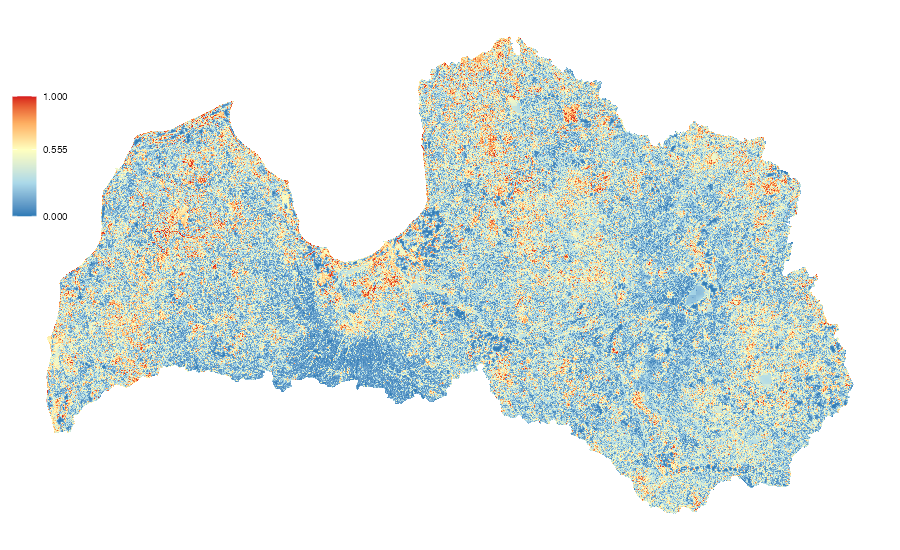
\includegraphics[width=1\linewidth,height=0.70\textheight,keepaspectratio]{results/LISVULv2a/PicHSmap_LISVUL.png}

\par\small\textit{Predicted continuous habitat suitability across Latvia. The warmer the colour the higher is the predicted habitat suitability. Value in the middle of the legend correspond to the maximum training sensitivity plus specificity threshold. **For a full resolution refer to repository: link or online document: link**}\normalsize
\end{center}

\section*{Model thresholds}\label{model-thresholds}
\addcontentsline{toc}{section}{Model thresholds}

Threshold values and associated omission rates

\begin{center}
\resizebox{\linewidth}{!}{%

\begin{tabular}{lrrrrr}
\toprule
Threshold & Cloglog value & Fractional predicted area & Training omission rate & Test omission rate & P-values\\
\midrule
Minimum training presence & 0.1096925 & 0.9228062 & 0.0000000 & 0.0000996 & 0\\
Equal training sensitivity and specificity & 0.5659657 & 0.2718218 & 0.2710280 & 0.0021912 & 0\\
Maximum training sensitivity plus specificity & 0.5547385 & 0.2851688 & 0.2523364 & 0.0020916 & 0\\
Equal test sensitivity and specificity & 0.5647520 & 0.2732162 & 0.2663551 & 0.0021912 & 0\\
Maximum test sensitivity plus specificity & 0.4786952 & 0.3811548 & 0.1869159 & 0.0009960 & 0\\
\bottomrule
\end{tabular}
}
\end{center}

\section*{Variable importance}\label{variable-importance}
\addcontentsline{toc}{section}{Variable importance}

\begin{center}
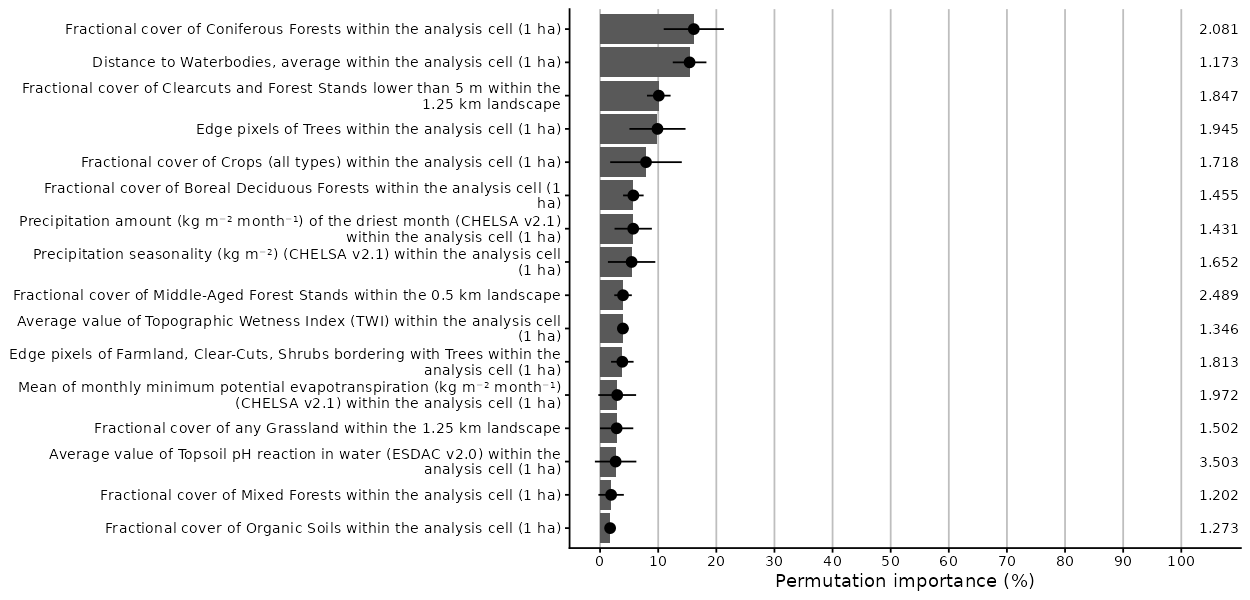
\includegraphics[width=1\linewidth,height=0.70\textheight,keepaspectratio]{results/LISVULv2a/PicVarImpVIFs_LISVUL.png}

\par\small\textit{Permutation-importance (mean and standard deviation from 99 permutations, on the x-axis) of the ecogeographical variables (first y-axis, left side), and their variance inflation factor values (second y-axis, right side). **For a full resolution refer to repository: link or online document: link**}\normalsize
\end{center}

\section*{Marginal responses}\label{marginal-responses}
\addcontentsline{toc}{section}{Marginal responses}

\begin{center}
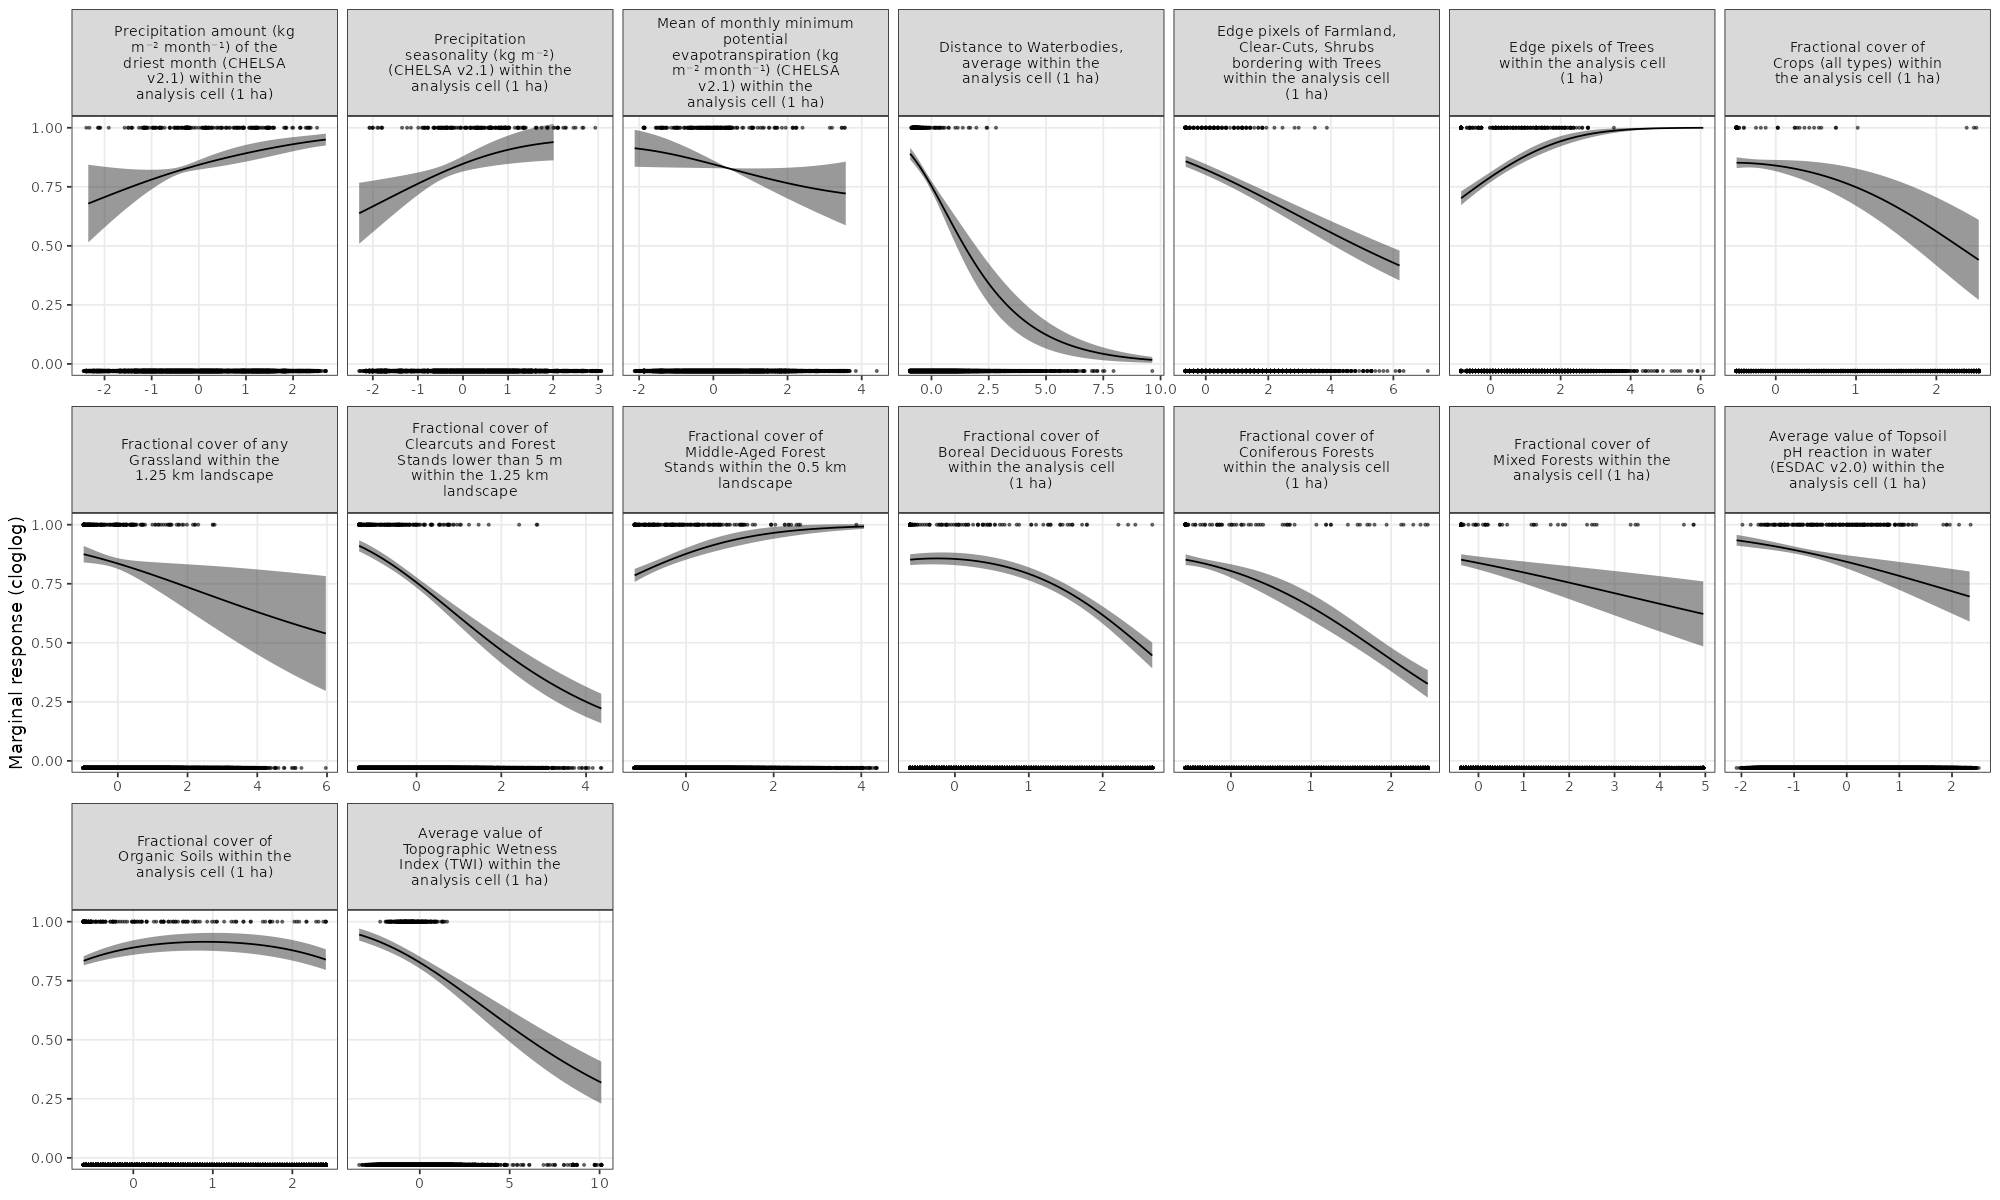
\includegraphics[width=1\linewidth,height=0.70\textheight,keepaspectratio]{results/LISVULv2a/PicMargResp_LISVUL.png}

\par\small\textit{Marginalised for arithmetic mean response curves illustrating the effect of each ecogeographical variable on the habitat suitability when all the other variables have their arithmetic mean values. The y-axis shows the predicted habitat suitability (cloglog-transformed), while the x-axis shows the standardised (centred and scaled) value of the ecogeographical variable. Dots at a value of 1 on the y-axis illustrate presence locations in the environment (on the x-axis), while dots at a value of 0 illustrate background locations used in modelling.  **For a full resolution refer to repository: link or online document: link**}\normalsize
\end{center}

\section*{Habitat and conservation associations}\label{habitat-and-conservation-associations}
\addcontentsline{toc}{section}{Habitat and conservation associations}

\begin{center}
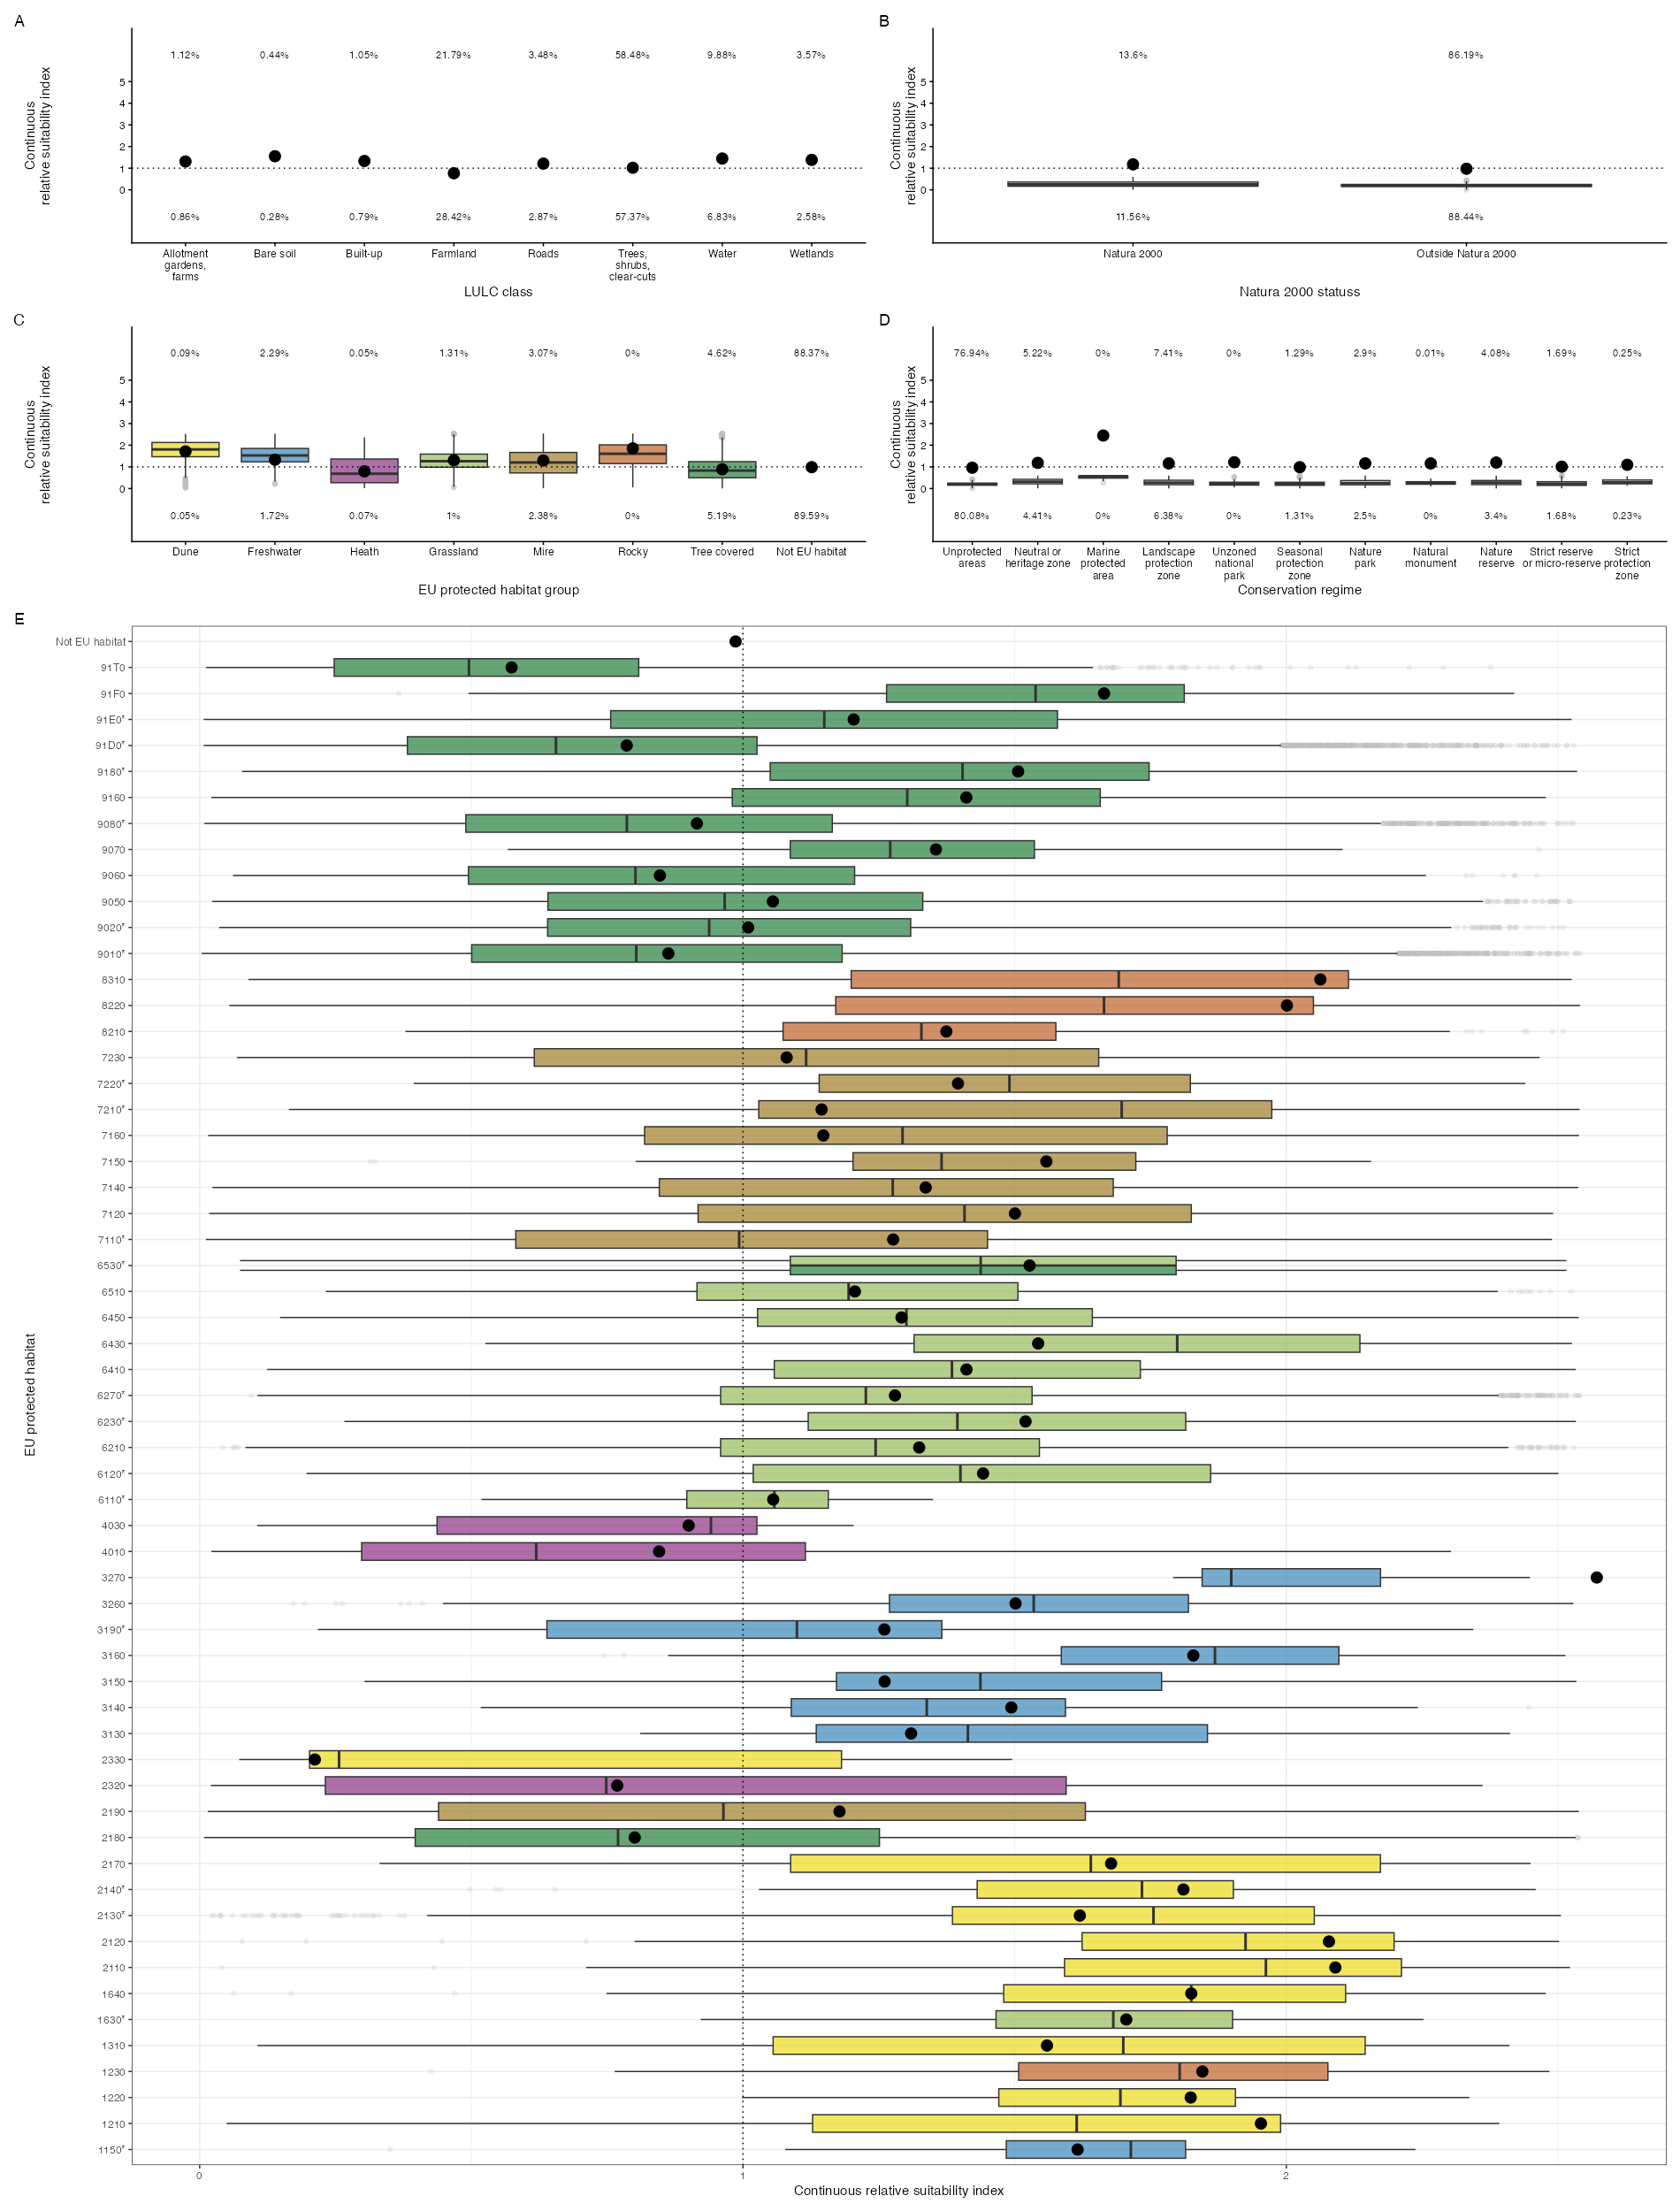
\includegraphics[width=1\linewidth,height=0.70\textheight,keepaspectratio]{results/LISVULv2a/PicAssoc_LISVUL.png}

\par\small\textit{Associations between predicted suitability and: (A) land use land cover classes, (B) Natura 2000 status, (C) stratified EU protected habitat classes, (D) conservation regime, and (E) EU protected habitats. The y-axis show continuous relative suitability index (derivative of Manly's index of preference). Colours in (C) and (E) correspond to stratified EU protected habitat classes. For classifications composed of multiple individual polygons, polygon-level indices were additionally calculated to show within-category variation. The figures therefore combine category-level estimates (points) with the distributions of polygon-level values (boxplots, where applicable). Labels above and below the panels report, respectively, the percentage of total predicted suitability and the percentage of mapped area represented by each category. **For a full resolution refer to repository: link or online document: link**}\normalsize
\end{center}

\section*{Conservation prioritization}\label{conservation-prioritization}
\addcontentsline{toc}{section}{Conservation prioritization}

\begin{center}
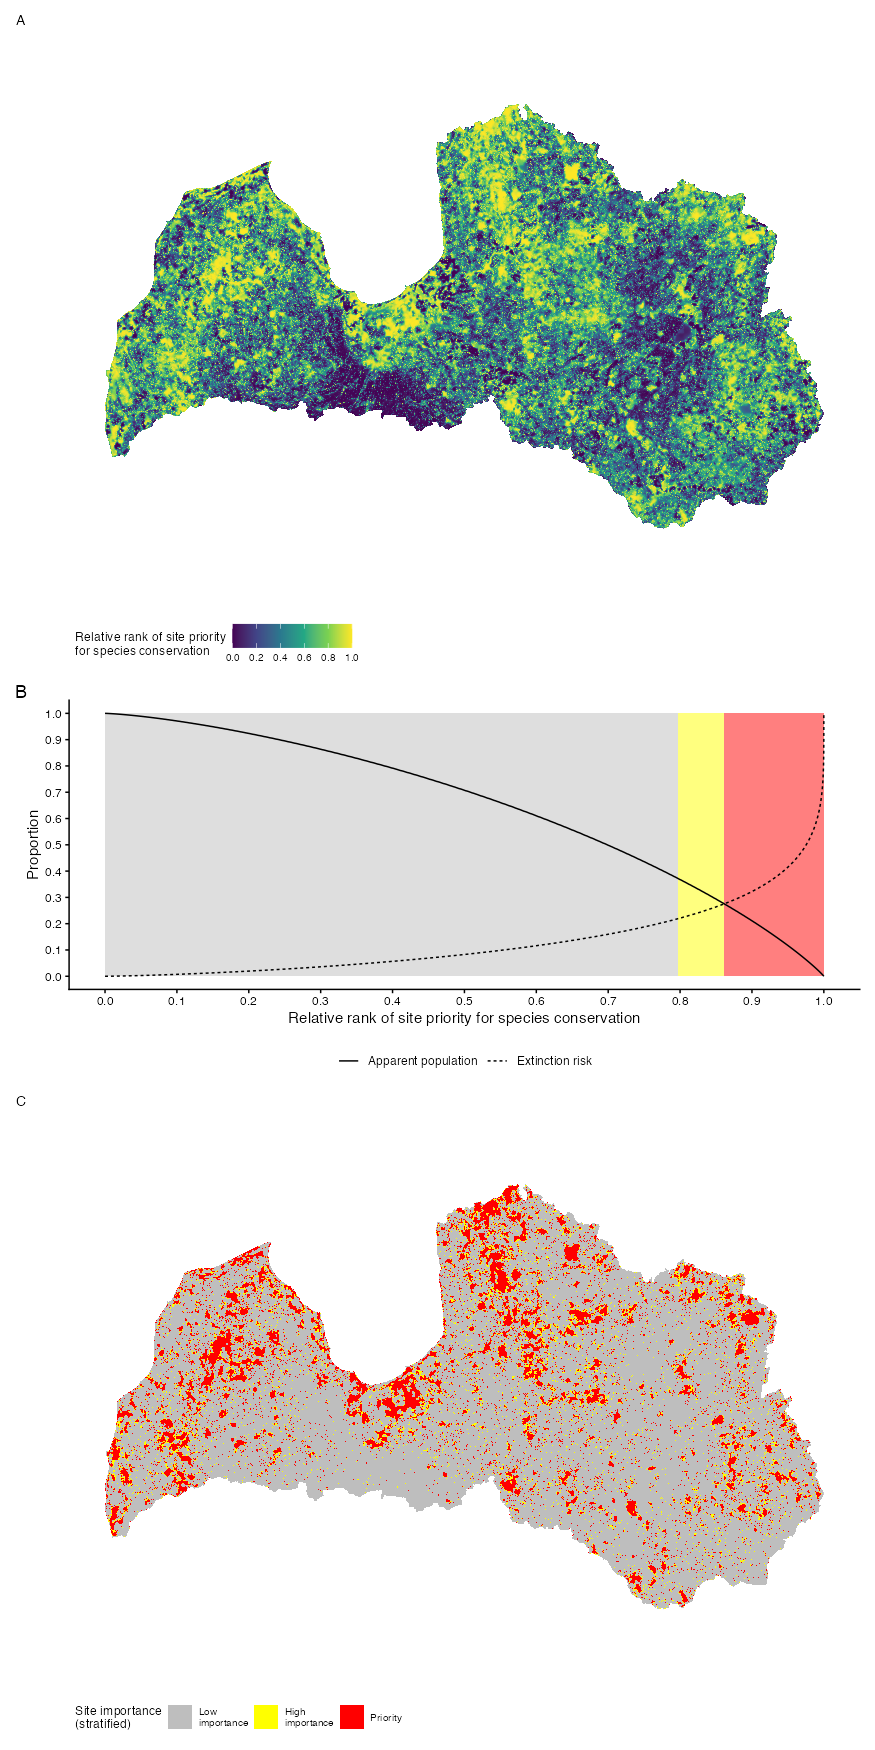
\includegraphics[width=0.85\linewidth,height=0.70\textheight,keepaspectratio]{results/LISVULv2a/PicPrior_LISVUL.png}

\par\small\textit{Single-species conservation prioritization focusing on maximisation of core area protection (CAZMAX) while accounting for site connectivity: (A) relative site rank; (B) relationship between apparent-population and extinction-risk curves with a simplified classification which is spatially demonstrated in the bootom row; (C) spatial distribution of proposed classification of site prioritization results. **For a full resolution refer to repository: link or online document: link**}\normalsize
\end{center}

\chapter*{\texorpdfstring{\emph{Lissotriton vulgaris} terrestrial}{Lissotriton vulgaris terrestrial}}\label{lisvulterrestrial}
\addcontentsline{toc}{chapter}{\emph{Lissotriton vulgaris} terrestrial}

\section*{Summary}\label{summary-1}
\addcontentsline{toc}{section}{Summary}

\subsection*{Model description}\label{model-description-1}
\addcontentsline{toc}{subsection}{Model description}

Occurrence and background data were divided into model-training with four block spatial cross-validation data and an independent test set. Sampling-bias/background treatment: \textbf{Phenology Weighted Target Group}. Accumulated LULC change within the 1-ha analysis cell was not evaluated; accumulated LULC change within the home-range radius around the analysis cell was not evaluated.

The final data set contained \textbf{139} presence records: \textbf{104} for training with four spatial block cross-validation and \textbf{35} for independent testing. Training background contained \textbf{29932} locations, with \textbf{10068} additional independent-test background locations.

\subsection*{Expert assessment scores}\label{expert-assessment-scores-1}
\addcontentsline{toc}{subsection}{Expert assessment scores}

\begin{itemize}
\tightlist
\item
  \textbf{Marginal responses and variable importance score:} 3 (moderate ecological interpretability)
\item
  \textbf{Map score:} 1 (poor agreement with known distribution)
\item
  \textbf{Applicability score:} 1 (very limited applicability)
\end{itemize}

\textbf{Šo sadaļu aizpildām manuāli no ekspertu aptaujām}

\subsection*{Statistical evaluation}\label{statistical-evaluation-1}
\addcontentsline{toc}{subsection}{Statistical evaluation}

The final model had a training TSS of \textbf{0.401}, with a training-derived cloglog threshold of \textbf{0.515}. Combined training AUC was \textbf{0.795} and combined test AUC was \textbf{0.714}.

\subsubsection*{Spatial cross-validation}\label{spatial-cross-validation-1}
\addcontentsline{toc}{subsubsection}{Spatial cross-validation}

\begin{itemize}
\tightlist
\item
  \textbf{AUC:} 0.7144 ± 0.0336; null models: 0.5202 ± 0.0304; z = 6.3858, p \textless{} 0.001
\item
  \textbf{CBI:} 0.8048 ± 0.0915; null models: 0.0622 ± 0.1508; z = 4.9234, p \textless{} 0.001
\item
  \textbf{OR10:} 0.2596 ± 0.192; null models: 0.1057 ± 0.0699; z = 2.201, p = 0.986
\item
  \textbf{ORmin:} 0.0481 ± 0.0728; null models: 0.0143 ± 0.0295; z = 1.1429, p = 0.873
\end{itemize}

\subsubsection*{Independent testing}\label{independent-testing-1}
\addcontentsline{toc}{subsubsection}{Independent testing}

\begin{itemize}
\tightlist
\item
  \textbf{TSS:} 0.326; \textbf{sensitivity:} 0.714; \textbf{specificity:} 0.612
\item
  \textbf{AUC:} 0.744; null models: 0.492 ± 0.0927; z = 2.7203, p = 0.003
\item
  \textbf{CBI:} 0.851; null models: -0.0041 ± 0.4729; z = 1.8083, p = 0.035
\item
  \textbf{OR10:} 0.114; null models: 0.144 ± 0.0986; z = -0.3013, p = 0.382
\item
  \textbf{ORmin:} 0; null models: 0.0191 ± 0.0352; z = -0.5441, p = 0.293
\end{itemize}

\subsection*{Conservation prioritisation summary}\label{conservation-prioritisation-summary-1}
\addcontentsline{toc}{subsection}{Conservation prioritisation summary}

The primary priority area covers \textbf{13.7\%} of Latvia and contains \textbf{27.6\%} of the summed habitat suitability (apparent population proxy).

The broader high importance area covers \textbf{23.6\%} of Latvia and contains \textbf{41.5\%} of the summed habitat suitability.

For comparison, the area classified as suitable using the maximum training sensitivity plus specificity habitat-suitability threshold contains \textbf{41.5\%} of the summed continuous habitat suitability.

\subsection*{Version evolution}\label{version-evolution-1}
\addcontentsline{toc}{subsection}{Version evolution}

\textbf{Šo sadaļu aizpildām manuāli, izmntojot sagatavotās shēmas. Jāvienojas par to noformējumu}

\section*{Habitat suitability}\label{habitat-suitability-1}
\addcontentsline{toc}{section}{Habitat suitability}

\begin{center}
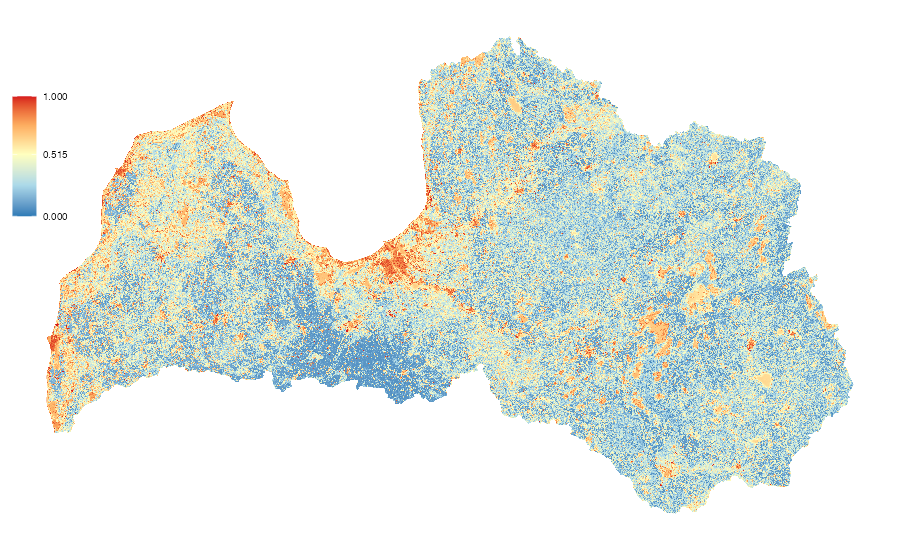
\includegraphics[width=1\linewidth,height=0.70\textheight,keepaspectratio]{results/LISVULterrestrialv4b1/PicHSmap_LISVULterrestrial.png}

\par\small\textit{Predicted continuous habitat suitability across Latvia. The warmer the colour the higher is the predicted habitat suitability. Value in the middle of the legend correspond to the maximum training sensitivity plus specificity threshold. **For a full resolution refer to repository: link or online document: link**}\normalsize
\end{center}

\section*{Model thresholds}\label{model-thresholds-1}
\addcontentsline{toc}{section}{Model thresholds}

Threshold values and associated omission rates

\begin{center}
\resizebox{\linewidth}{!}{%

\begin{tabular}{lrrrrr}
\toprule
Threshold & Cloglog value & Fractional predicted area & Training omission rate & Test omission rate & P-values\\
\midrule
Minimum training presence & 0.1472103 & 0.8486983 & 0.0000000 & 0.0000000 & 0\\
Equal training sensitivity and specificity & 0.5587244 & 0.2884513 & 0.2884615 & 0.0011864 & 0\\
Maximum training sensitivity plus specificity & 0.5151853 & 0.3444593 & 0.1923077 & 0.0009886 & 0\\
Equal test sensitivity and specificity & 0.5538012 & 0.2955274 & 0.2884615 & 0.0011864 & 0\\
Maximum test sensitivity plus specificity & 0.4414090 & 0.4482310 & 0.1346154 & 0.0003955 & 0\\
\bottomrule
\end{tabular}
}
\end{center}

\section*{Variable importance}\label{variable-importance-1}
\addcontentsline{toc}{section}{Variable importance}

\begin{center}
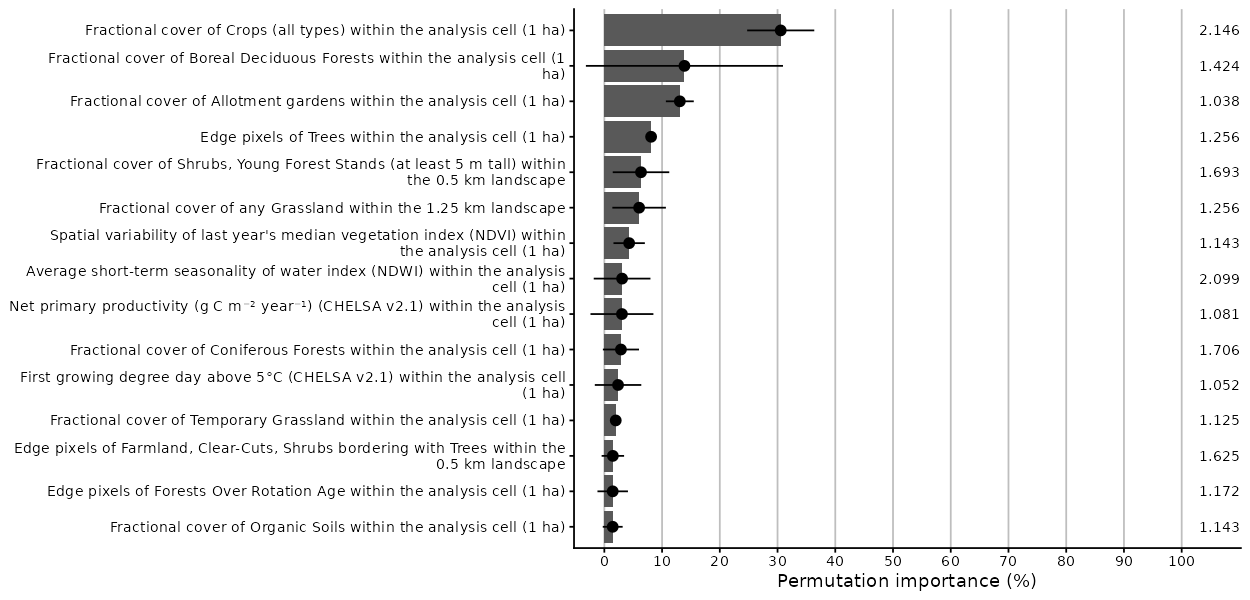
\includegraphics[width=1\linewidth,height=0.70\textheight,keepaspectratio]{results/LISVULterrestrialv4b1/PicVarImpVIFs_LISVULterrestrial.png}

\par\small\textit{Permutation-importance (mean and standard deviation from 99 permutations, on the x-axis) of the ecogeographical variables (first y-axis, left side), and their variance inflation factor values (second y-axis, right side). **For a full resolution refer to repository: link or online document: link**}\normalsize
\end{center}

\section*{Marginal responses}\label{marginal-responses-1}
\addcontentsline{toc}{section}{Marginal responses}

\begin{center}
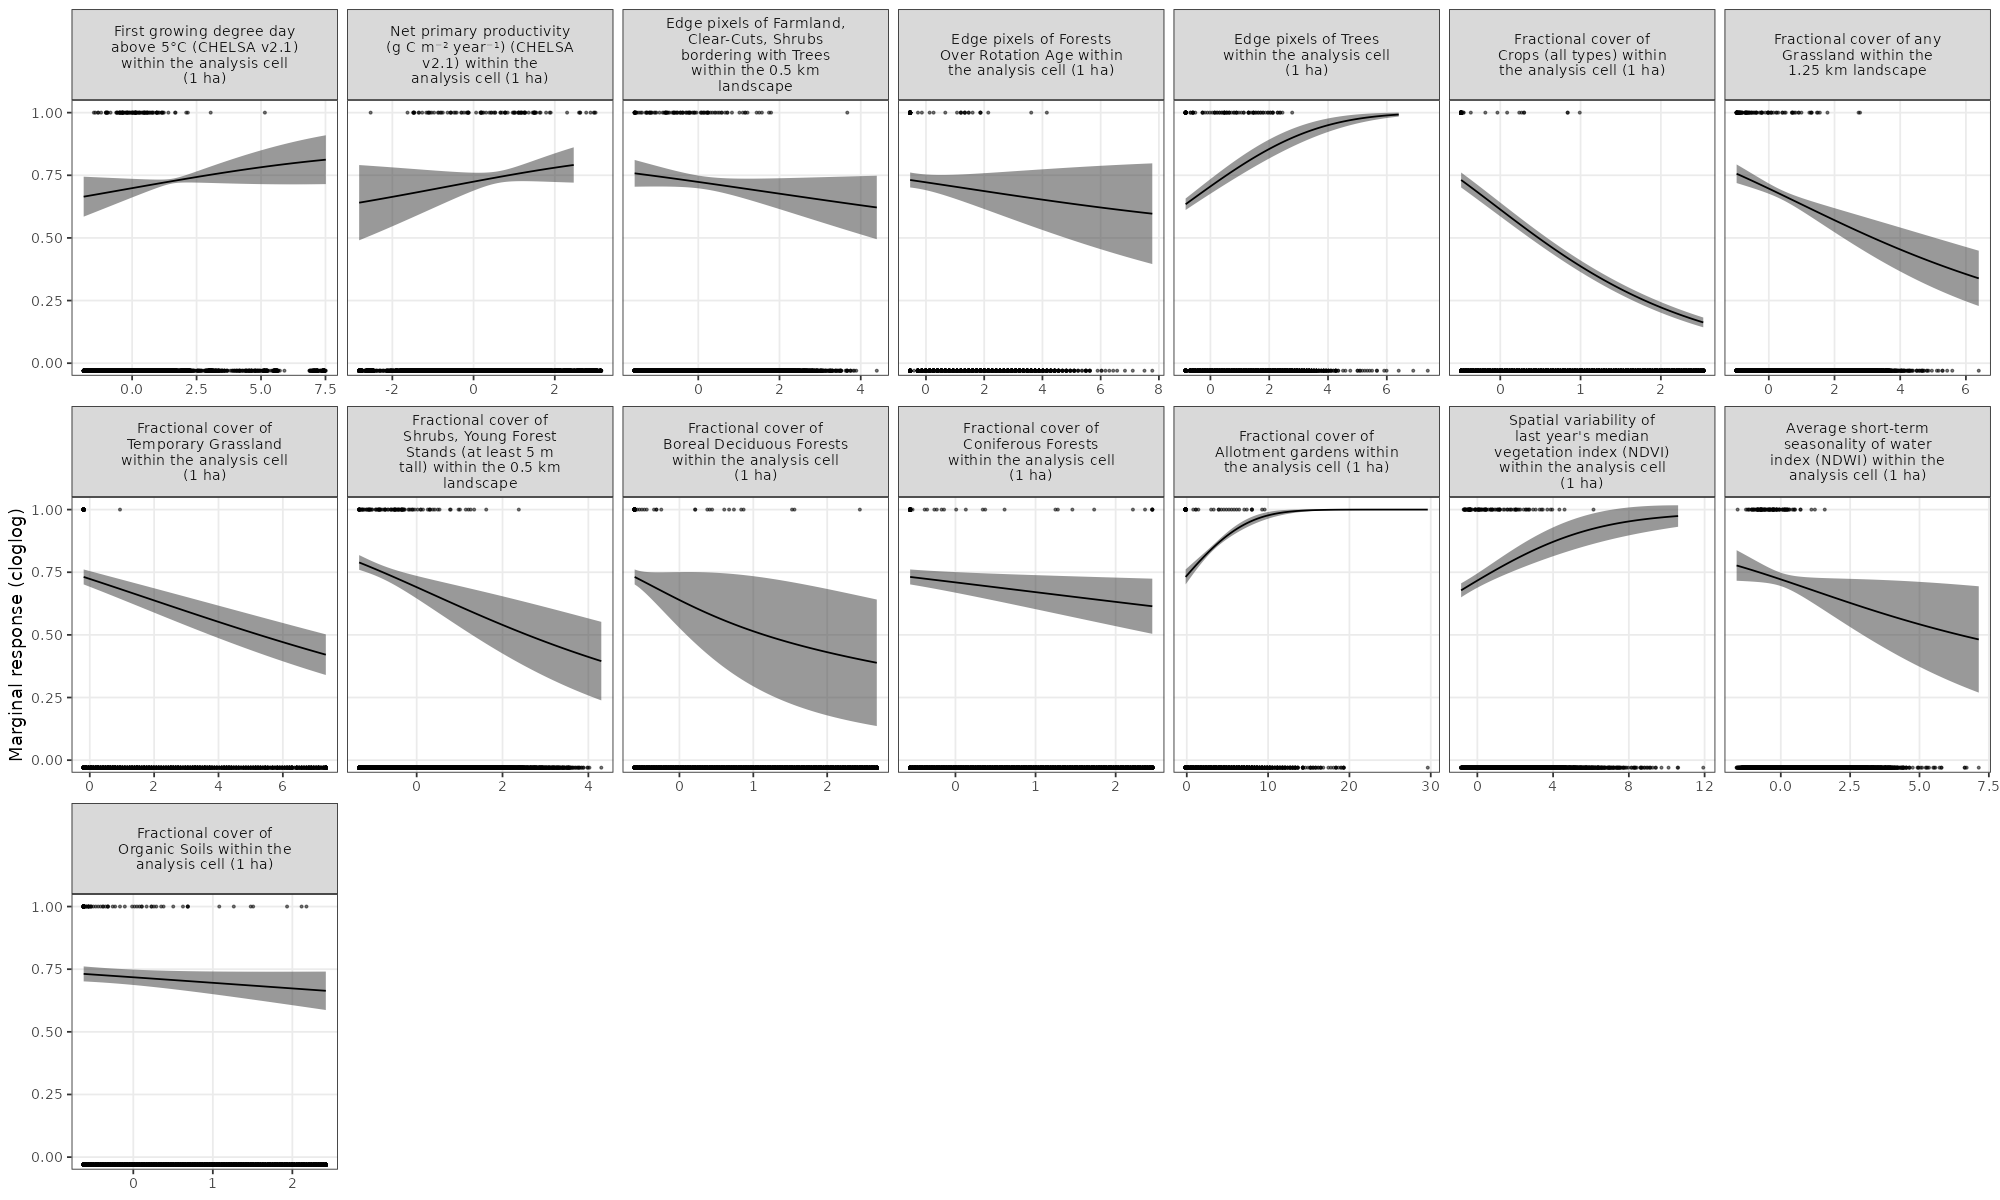
\includegraphics[width=1\linewidth,height=0.70\textheight,keepaspectratio]{results/LISVULterrestrialv4b1/PicMargResp_LISVULterrestrial.png}

\par\small\textit{Marginalised for arithmetic mean response curves illustrating the effect of each ecogeographical variable on the habitat suitability when all the other variables have their arithmetic mean values. The y-axis shows the predicted habitat suitability (cloglog-transformed), while the x-axis shows the standardised (centred and scaled) value of the ecogeographical variable. Dots at a value of 1 on the y-axis illustrate presence locations in the environment (on the x-axis), while dots at a value of 0 illustrate background locations used in modelling.  **For a full resolution refer to repository: link or online document: link**}\normalsize
\end{center}

\section*{Habitat and conservation associations}\label{habitat-and-conservation-associations-1}
\addcontentsline{toc}{section}{Habitat and conservation associations}

\begin{center}
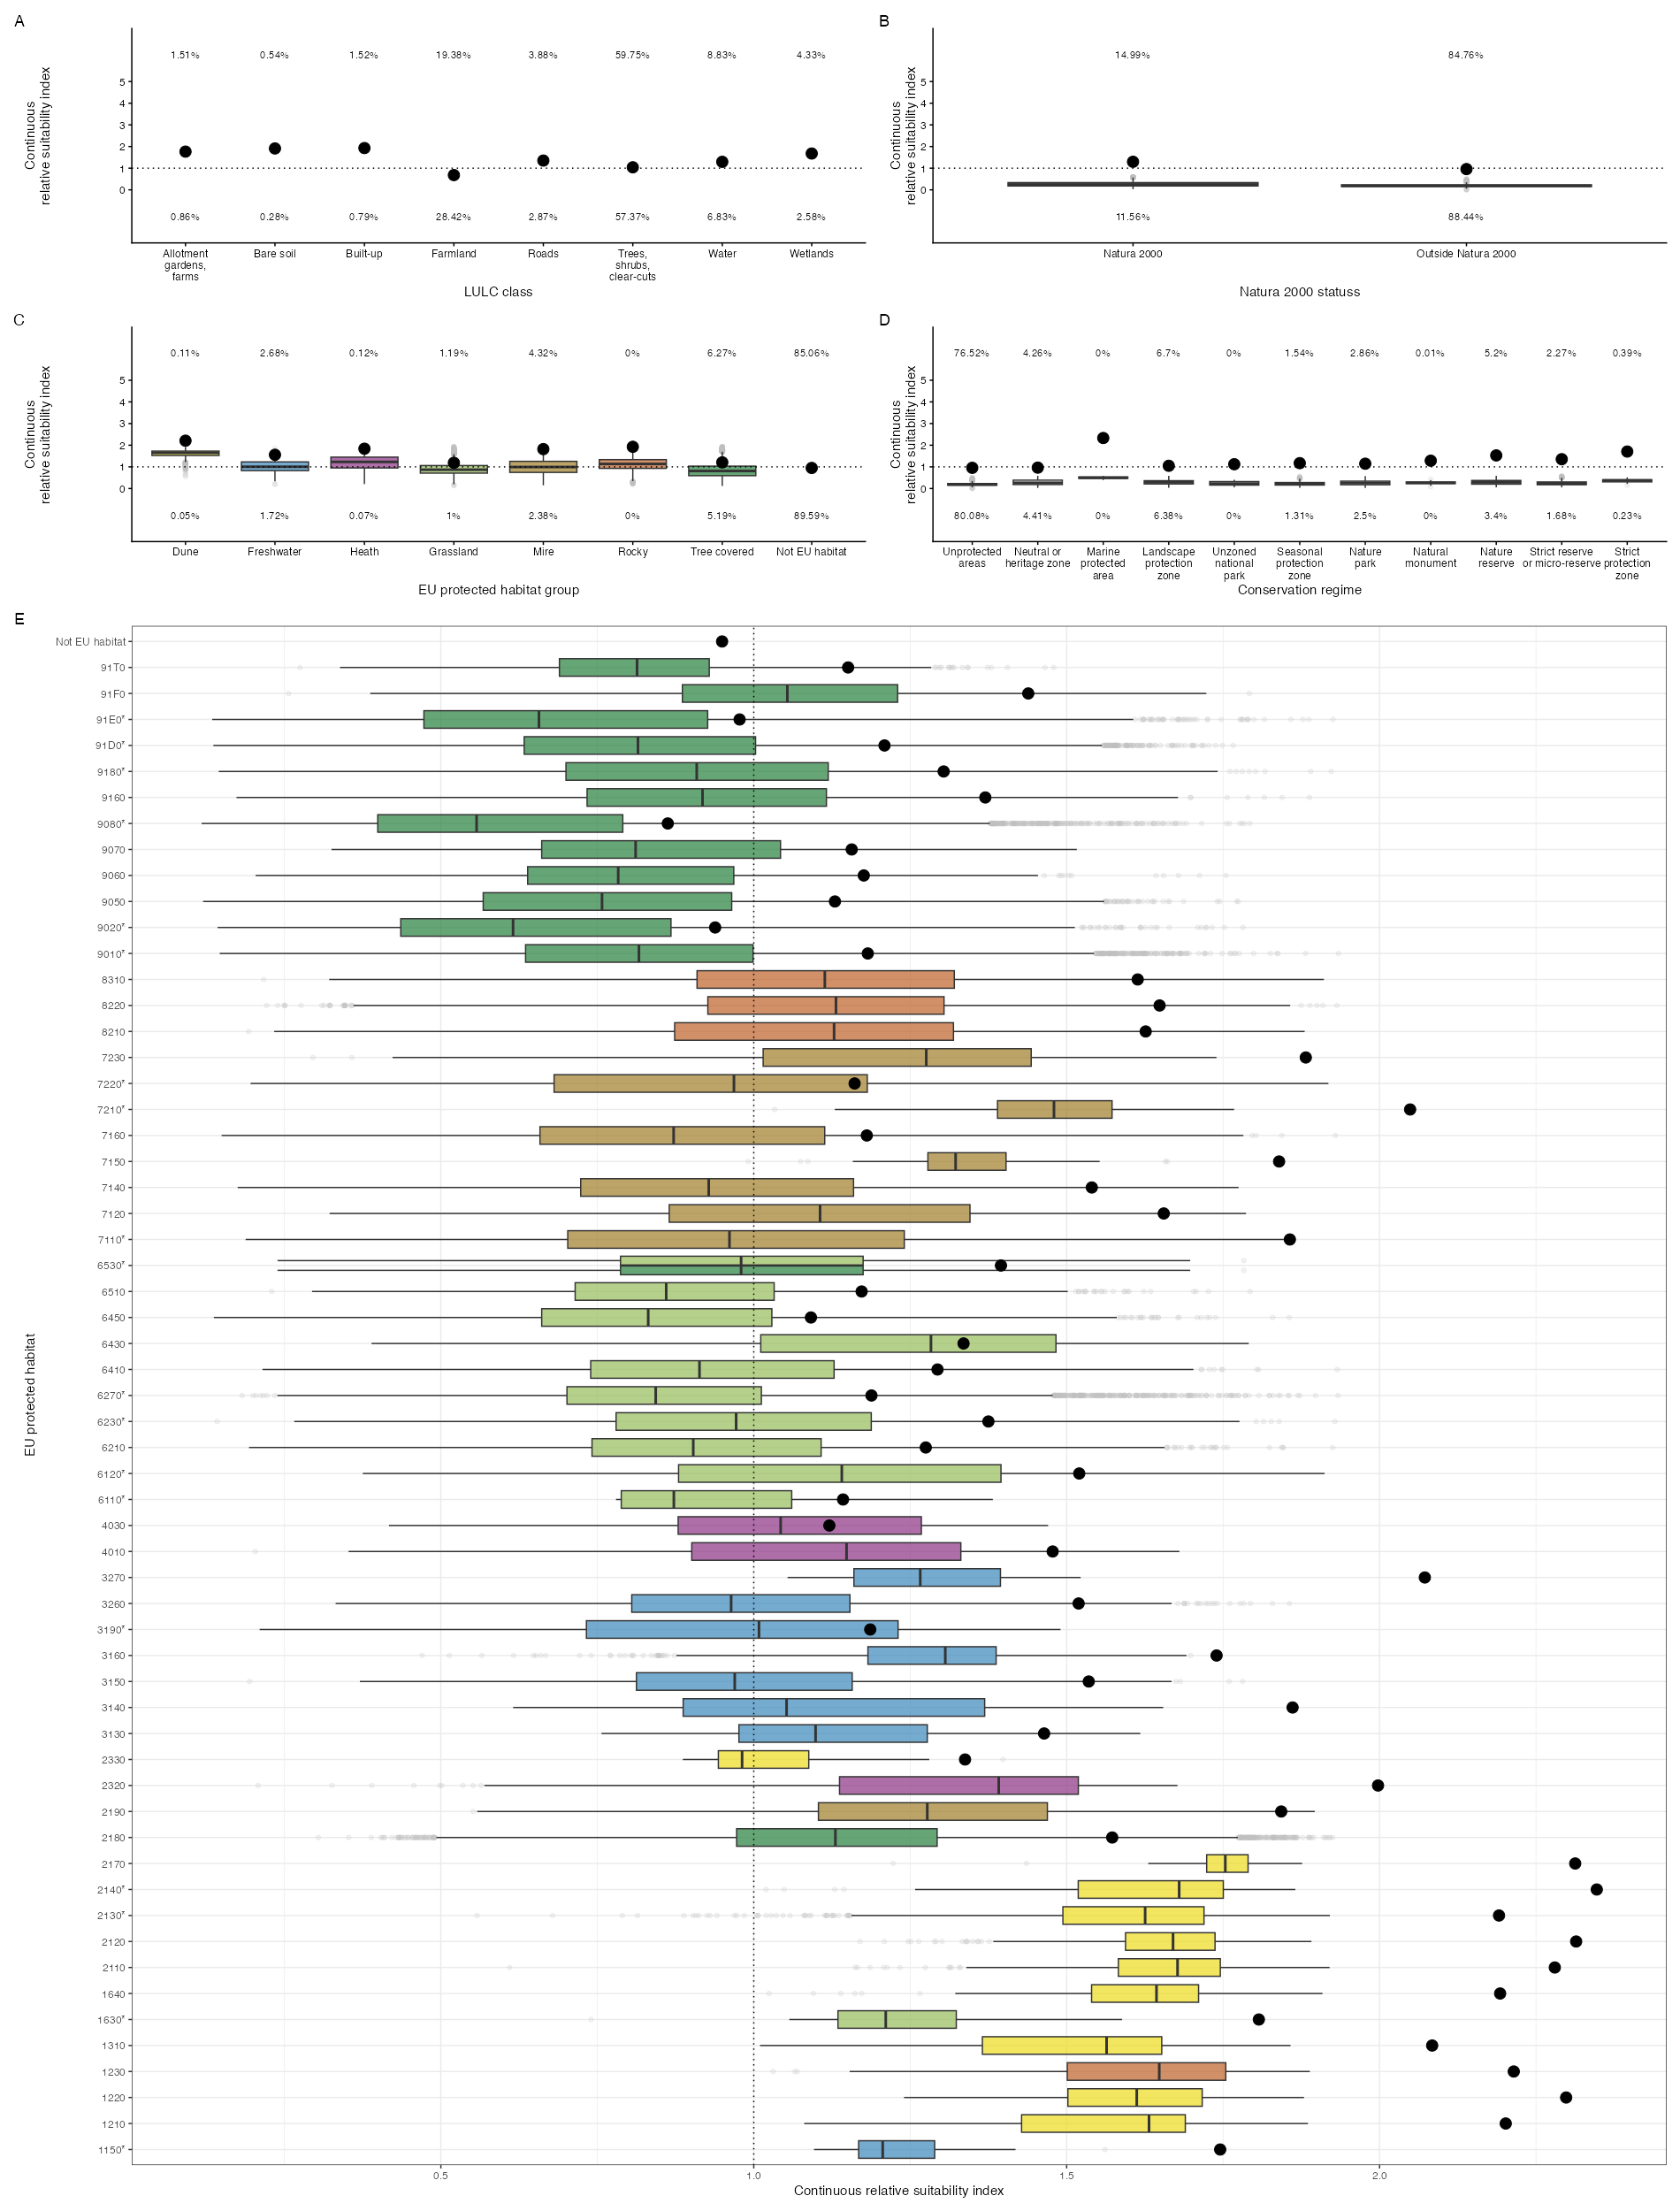
\includegraphics[width=1\linewidth,height=0.70\textheight,keepaspectratio]{results/LISVULterrestrialv4b1/PicAssoc_LISVULterrestrial.png}

\par\small\textit{Associations between predicted suitability and: (A) land use land cover classes, (B) Natura 2000 status, (C) stratified EU protected habitat classes, (D) conservation regime, and (E) EU protected habitats. The y-axis show continuous relative suitability index (derivative of Manly's index of preference). Colours in (C) and (E) correspond to stratified EU protected habitat classes. For classifications composed of multiple individual polygons, polygon-level indices were additionally calculated to show within-category variation. The figures therefore combine category-level estimates (points) with the distributions of polygon-level values (boxplots, where applicable). Labels above and below the panels report, respectively, the percentage of total predicted suitability and the percentage of mapped area represented by each category. **For a full resolution refer to repository: link or online document: link**}\normalsize
\end{center}

\section*{Conservation prioritization}\label{conservation-prioritization-1}
\addcontentsline{toc}{section}{Conservation prioritization}

\begin{center}
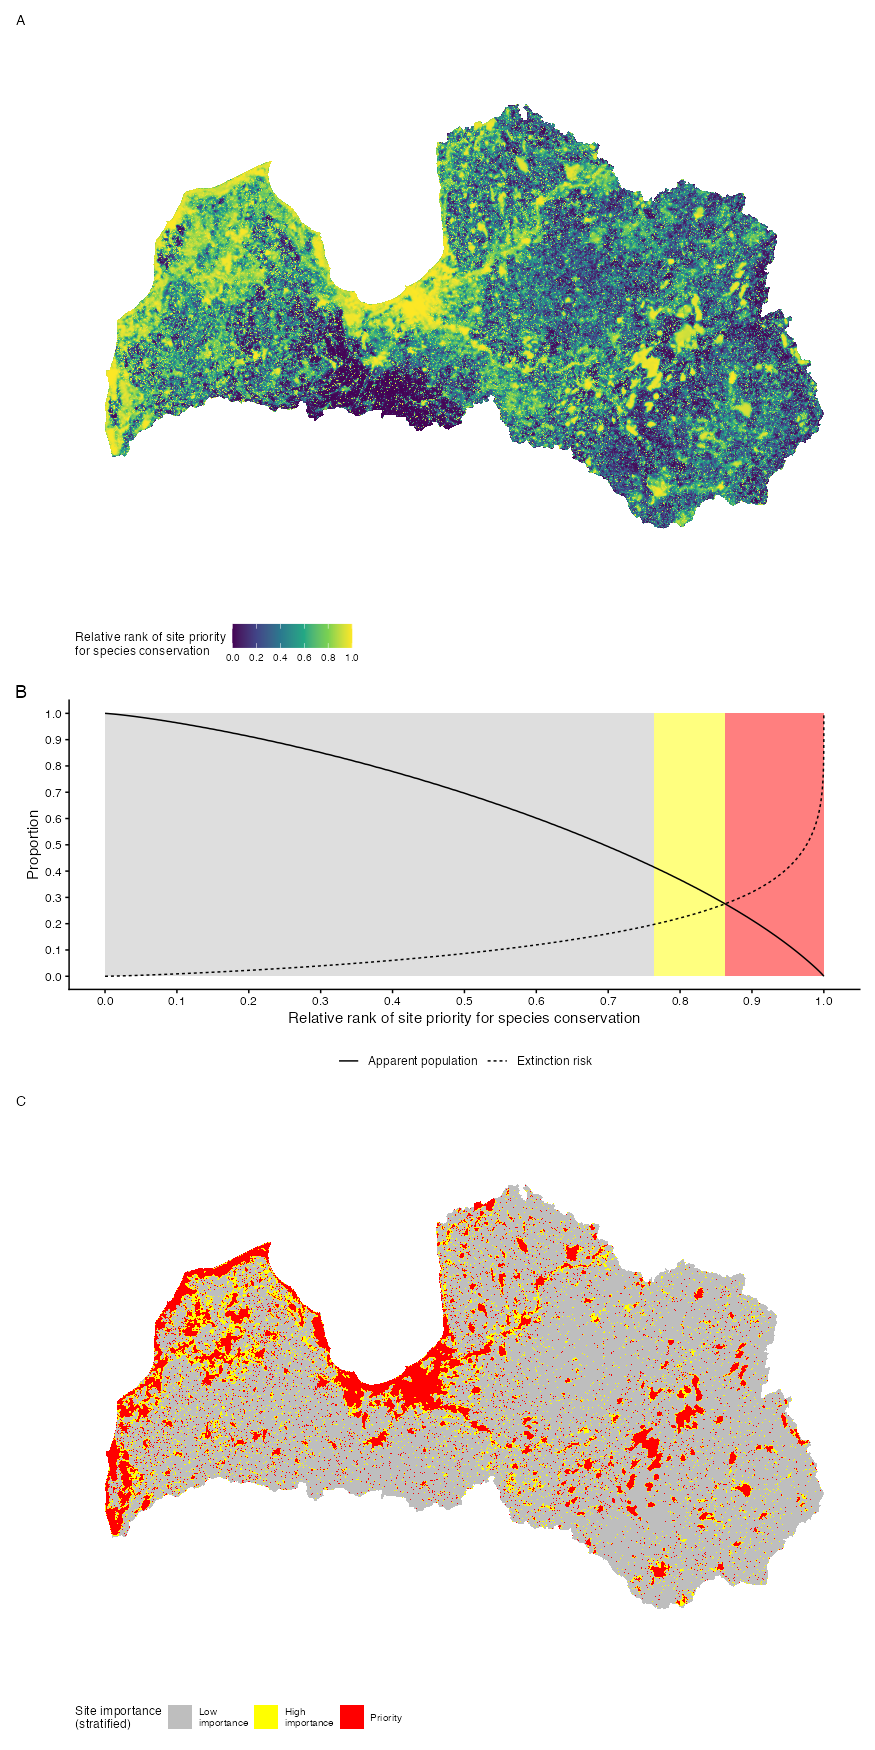
\includegraphics[width=0.85\linewidth,height=0.70\textheight,keepaspectratio]{results/LISVULterrestrialv4b1/PicPrior_LISVULterrestrial.png}

\par\small\textit{Single-species conservation prioritization focusing on maximisation of core area protection (CAZMAX) while accounting for site connectivity: (A) relative site rank; (B) relationship between apparent-population and extinction-risk curves with a simplified classification which is spatially demonstrated in the bootom row; (C) spatial distribution of proposed classification of site prioritization results. **For a full resolution refer to repository: link or online document: link**}\normalsize
\end{center}

\chapter*{\texorpdfstring{\emph{Lissotriton vulgaris} larvae}{Lissotriton vulgaris larvae}}\label{lisvullarvae}
\addcontentsline{toc}{chapter}{\emph{Lissotriton vulgaris} larvae}

\section*{Summary}\label{summary-2}
\addcontentsline{toc}{section}{Summary}

\subsection*{Model description}\label{model-description-2}
\addcontentsline{toc}{subsection}{Model description}

Occurrence and background data were divided into model-training with four block spatial cross-validation data and an independent test set. Sampling-bias/background treatment: \textbf{Phenology Weighted Target Group}. Observations were retained only where accumulated LULC change within the 1-ha analysis cell from the year of observation to 2024 did not exceed 50\%; observations were retained only where accumulated LULC change within the home-range radius around the analysis cell from the year of observation to 2024 did not exceed 50\%.

The final data set contained \textbf{280} presence records: \textbf{210} for training with four spatial block cross-validation and \textbf{70} for independent testing. Training background contained \textbf{30006} locations, with \textbf{9994} additional independent-test background locations.

\subsection*{Expert assessment scores}\label{expert-assessment-scores-2}
\addcontentsline{toc}{subsection}{Expert assessment scores}

\begin{itemize}
\tightlist
\item
  \textbf{Marginal responses and variable importance score:} 4 (good ecological interpretability)
\item
  \textbf{Map score:} 2 (limited agreement with known distribution)
\item
  \textbf{Applicability score:} 3 (moderate applicability)
\end{itemize}

\textbf{Šo sadaļu aizpildām manuāli no ekspertu aptaujām}

\subsection*{Statistical evaluation}\label{statistical-evaluation-2}
\addcontentsline{toc}{subsection}{Statistical evaluation}

The final model had a training TSS of \textbf{0.401}, with a training-derived cloglog threshold of \textbf{0.551}. Combined training AUC was \textbf{0.831} and combined test AUC was \textbf{0.809}.

\subsubsection*{Spatial cross-validation}\label{spatial-cross-validation-2}
\addcontentsline{toc}{subsubsection}{Spatial cross-validation}

\begin{itemize}
\tightlist
\item
  \textbf{AUC:} 0.8078 ± 0.0425; null models: 0.4971 ± 0.0253; z = 12.2709, p \textless{} 0.001
\item
  \textbf{CBI:} 0.9388 ± 0.0378; null models: -0.026 ± 0.139; z = 6.9391, p \textless{} 0.001
\item
  \textbf{OR10:} 0.1568 ± 0.0486; null models: 0.1315 ± 0.0655; z = 0.3874, p = 0.651
\item
  \textbf{ORmin:} 0.0142 ± 0.0181; null models: 0.015 ± 0.0433; z = -0.0183, p = 0.493
\end{itemize}

\subsubsection*{Independent testing}\label{independent-testing-2}
\addcontentsline{toc}{subsubsection}{Independent testing}

\begin{itemize}
\tightlist
\item
  \textbf{TSS:} 0.494; \textbf{sensitivity:} 0.786; \textbf{specificity:} 0.708
\item
  \textbf{AUC:} 0.82; null models: 0.4912 ± 0.0945; z = 3.4733, p \textless{} 0.001
\item
  \textbf{CBI:} 0.973; null models: -0.0728 ± 0.4683; z = 2.2334, p = 0.013
\item
  \textbf{OR10:} 0.1; null models: 0.1296 ± 0.0915; z = -0.3231, p = 0.373
\item
  \textbf{ORmin:} 0.029; null models: 0.0047 ± 0.0141; z = 1.6949, p = 0.955
\end{itemize}

\subsection*{Conservation prioritisation summary}\label{conservation-prioritisation-summary-2}
\addcontentsline{toc}{subsection}{Conservation prioritisation summary}

The primary priority area covers \textbf{15.6\%} of Latvia and contains \textbf{27.6\%} of the summed habitat suitability (apparent population proxy).

The broader high importance area covers \textbf{21.2\%} of Latvia and contains \textbf{35.3\%} of the summed habitat suitability.

For comparison, the area classified as suitable using the maximum training sensitivity plus specificity habitat-suitability threshold contains \textbf{35.3\%} of the summed continuous habitat suitability.

\subsection*{Version evolution}\label{version-evolution-2}
\addcontentsline{toc}{subsection}{Version evolution}

\textbf{Šo sadaļu aizpildām manuāli, izmntojot sagatavotās shēmas. Jāvienojas par to noformējumu}

\section*{Habitat suitability}\label{habitat-suitability-2}
\addcontentsline{toc}{section}{Habitat suitability}

\begin{center}
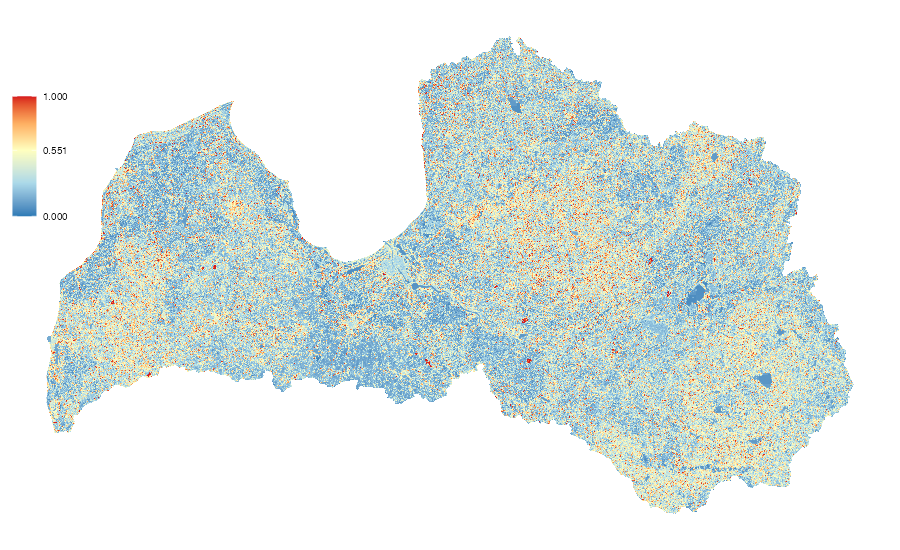
\includegraphics[width=1\linewidth,height=0.70\textheight,keepaspectratio]{results/LISVULlarvaev4a1/PicHSmap_LISVULlarvae.png}

\par\small\textit{Predicted continuous habitat suitability across Latvia. The warmer the colour the higher is the predicted habitat suitability. Value in the middle of the legend correspond to the maximum training sensitivity plus specificity threshold. **For a full resolution refer to repository: link or online document: link**}\normalsize
\end{center}

\section*{Model thresholds}\label{model-thresholds-2}
\addcontentsline{toc}{section}{Model thresholds}

Threshold values and associated omission rates

\begin{center}
\resizebox{\linewidth}{!}{%

\begin{tabular}{lrrrrr}
\toprule
Threshold & Cloglog value & Fractional predicted area & Training omission rate & Test omission rate & P-values\\
\midrule
Minimum training presence & 0.2414335 & 0.7567091 & 0.0000000 & 0.0001985 & 0\\
Equal training sensitivity and specificity & 0.5787267 & 0.2380968 & 0.2380952 & 0.0019851 & 0\\
Maximum training sensitivity plus specificity & 0.5514468 & 0.2690950 & 0.1952381 & 0.0014888 & 0\\
Equal test sensitivity and specificity & 0.5646598 & 0.2540121 & 0.2285714 & 0.0018859 & 0\\
Maximum test sensitivity plus specificity & 0.5464123 & 0.2750882 & 0.1952381 & 0.0013896 & 0\\
\bottomrule
\end{tabular}
}
\end{center}

\section*{Variable importance}\label{variable-importance-2}
\addcontentsline{toc}{section}{Variable importance}

\begin{center}
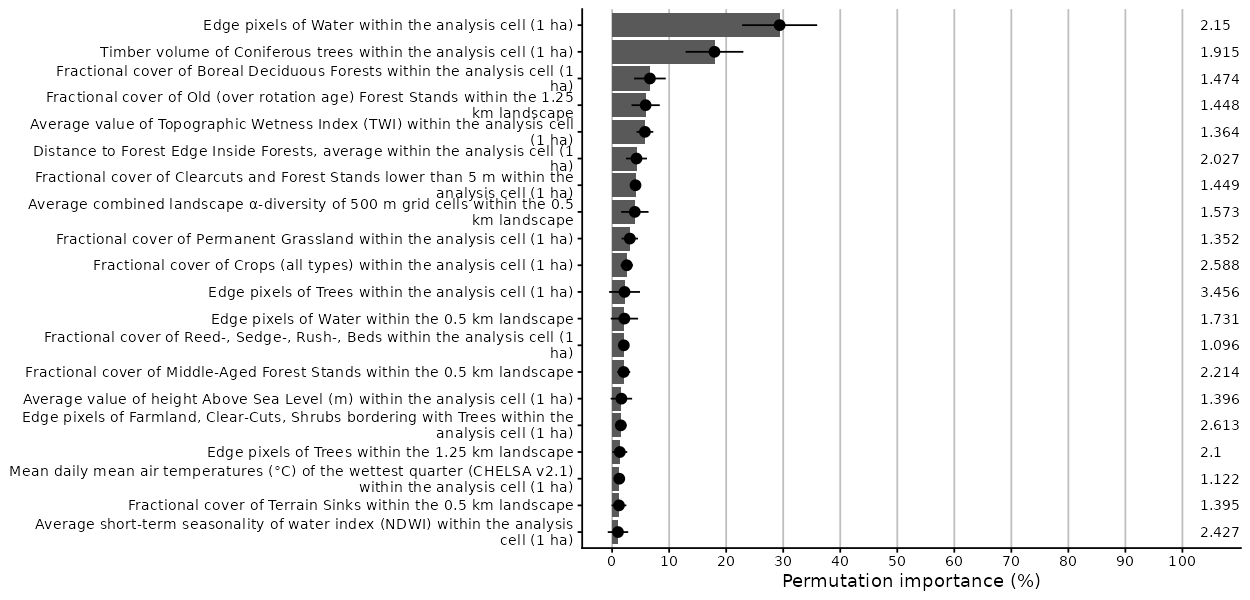
\includegraphics[width=1\linewidth,height=0.70\textheight,keepaspectratio]{results/LISVULlarvaev4a1/PicVarImpVIFs_LISVULlarvae.png}

\par\small\textit{Permutation-importance (mean and standard deviation from 99 permutations, on the x-axis) of the ecogeographical variables (first y-axis, left side), and their variance inflation factor values (second y-axis, right side). **For a full resolution refer to repository: link or online document: link**}\normalsize
\end{center}

\section*{Marginal responses}\label{marginal-responses-2}
\addcontentsline{toc}{section}{Marginal responses}

\begin{center}
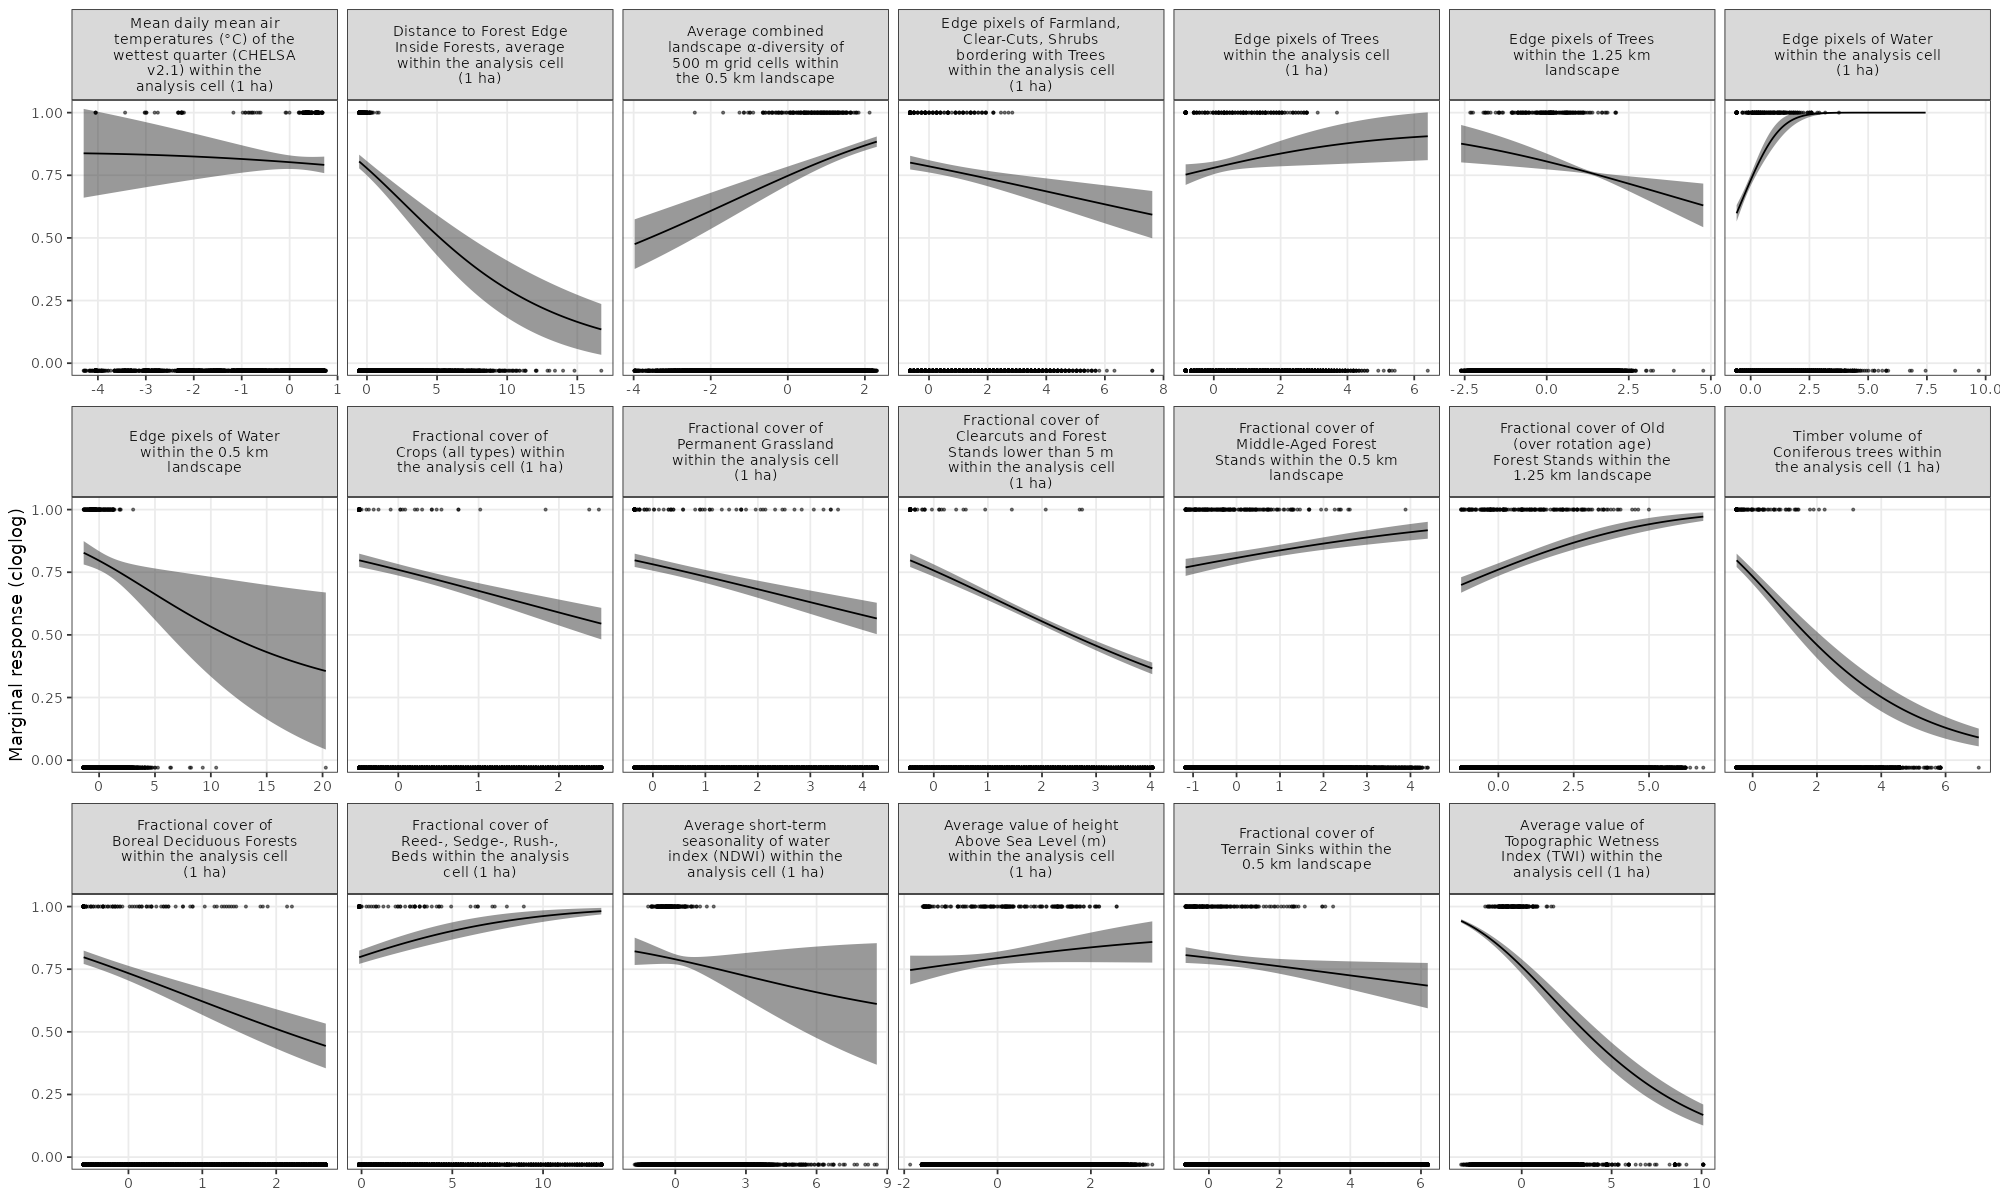
\includegraphics[width=1\linewidth,height=0.70\textheight,keepaspectratio]{results/LISVULlarvaev4a1/PicMargResp_LISVULlarvae.png}

\par\small\textit{Marginalised for arithmetic mean response curves illustrating the effect of each ecogeographical variable on the habitat suitability when all the other variables have their arithmetic mean values. The y-axis shows the predicted habitat suitability (cloglog-transformed), while the x-axis shows the standardised (centred and scaled) value of the ecogeographical variable. Dots at a value of 1 on the y-axis illustrate presence locations in the environment (on the x-axis), while dots at a value of 0 illustrate background locations used in modelling.  **For a full resolution refer to repository: link or online document: link**}\normalsize
\end{center}

\section*{Habitat and conservation associations}\label{habitat-and-conservation-associations-2}
\addcontentsline{toc}{section}{Habitat and conservation associations}

\begin{center}
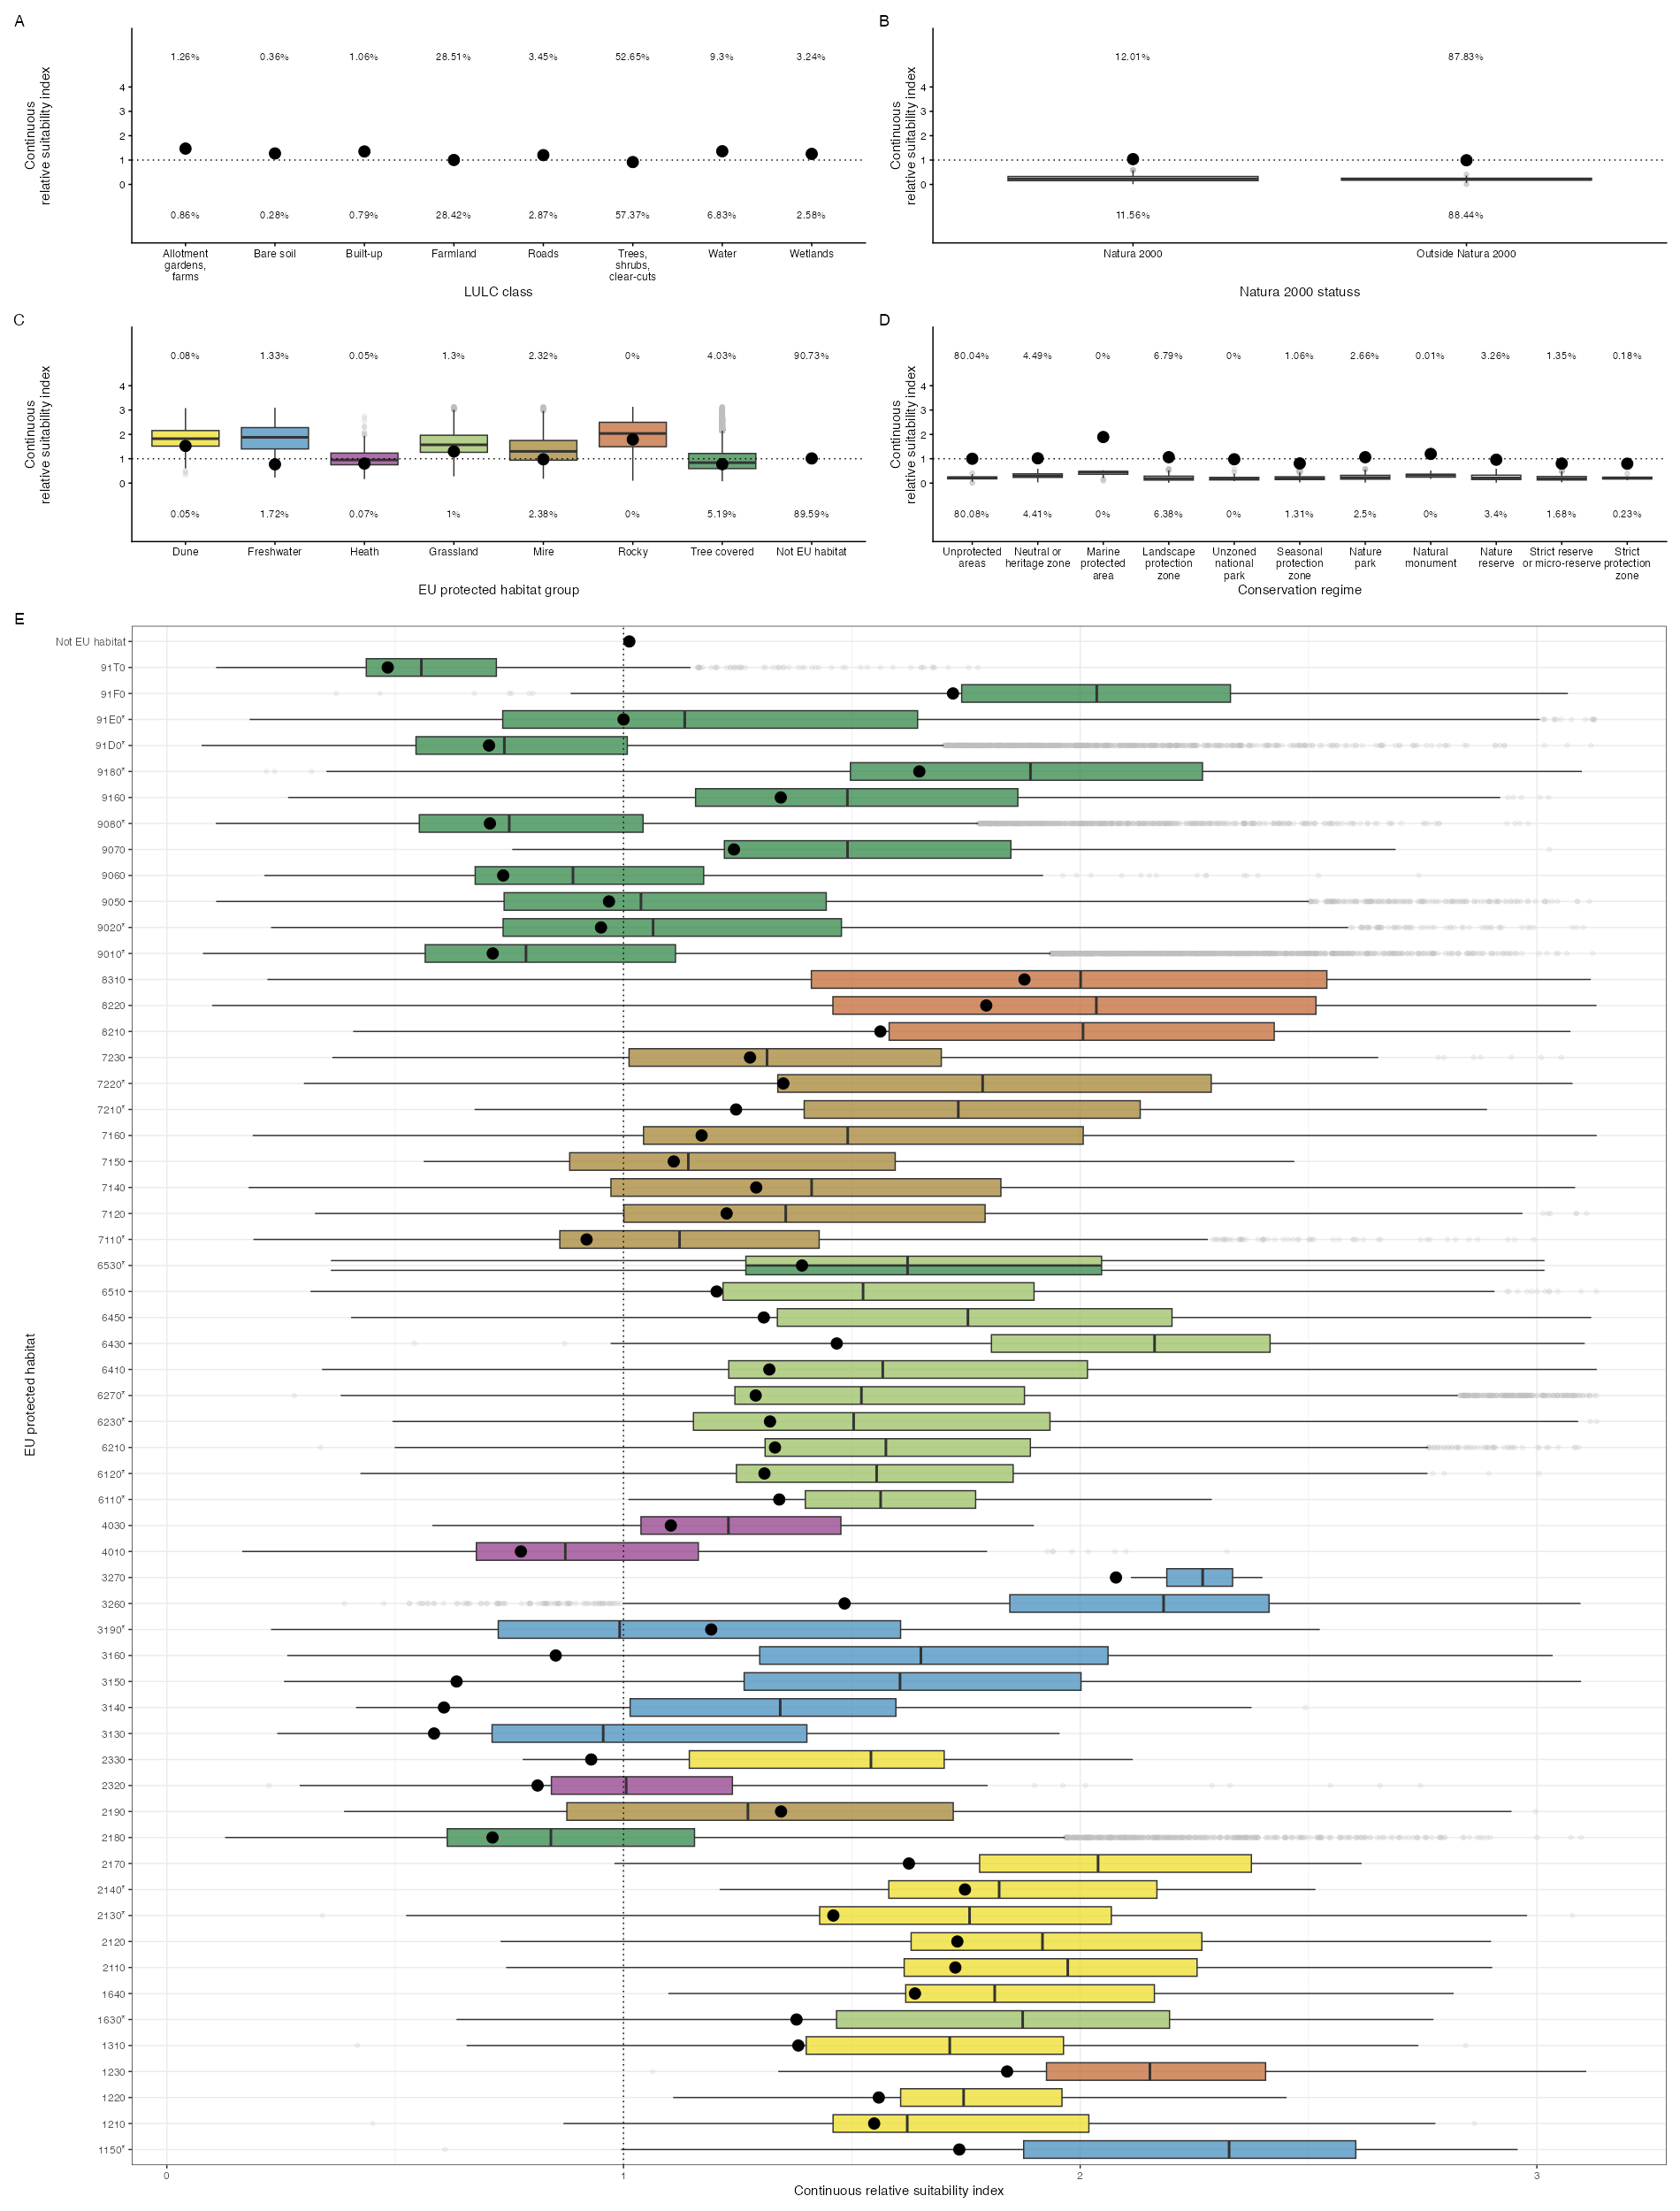
\includegraphics[width=1\linewidth,height=0.70\textheight,keepaspectratio]{results/LISVULlarvaev4a1/PicAssoc_LISVULlarvae.png}

\par\small\textit{Associations between predicted suitability and: (A) land use land cover classes, (B) Natura 2000 status, (C) stratified EU protected habitat classes, (D) conservation regime, and (E) EU protected habitats. The y-axis show continuous relative suitability index (derivative of Manly's index of preference). Colours in (C) and (E) correspond to stratified EU protected habitat classes. For classifications composed of multiple individual polygons, polygon-level indices were additionally calculated to show within-category variation. The figures therefore combine category-level estimates (points) with the distributions of polygon-level values (boxplots, where applicable). Labels above and below the panels report, respectively, the percentage of total predicted suitability and the percentage of mapped area represented by each category. **For a full resolution refer to repository: link or online document: link**}\normalsize
\end{center}

\section*{Conservation prioritization}\label{conservation-prioritization-2}
\addcontentsline{toc}{section}{Conservation prioritization}

\begin{center}
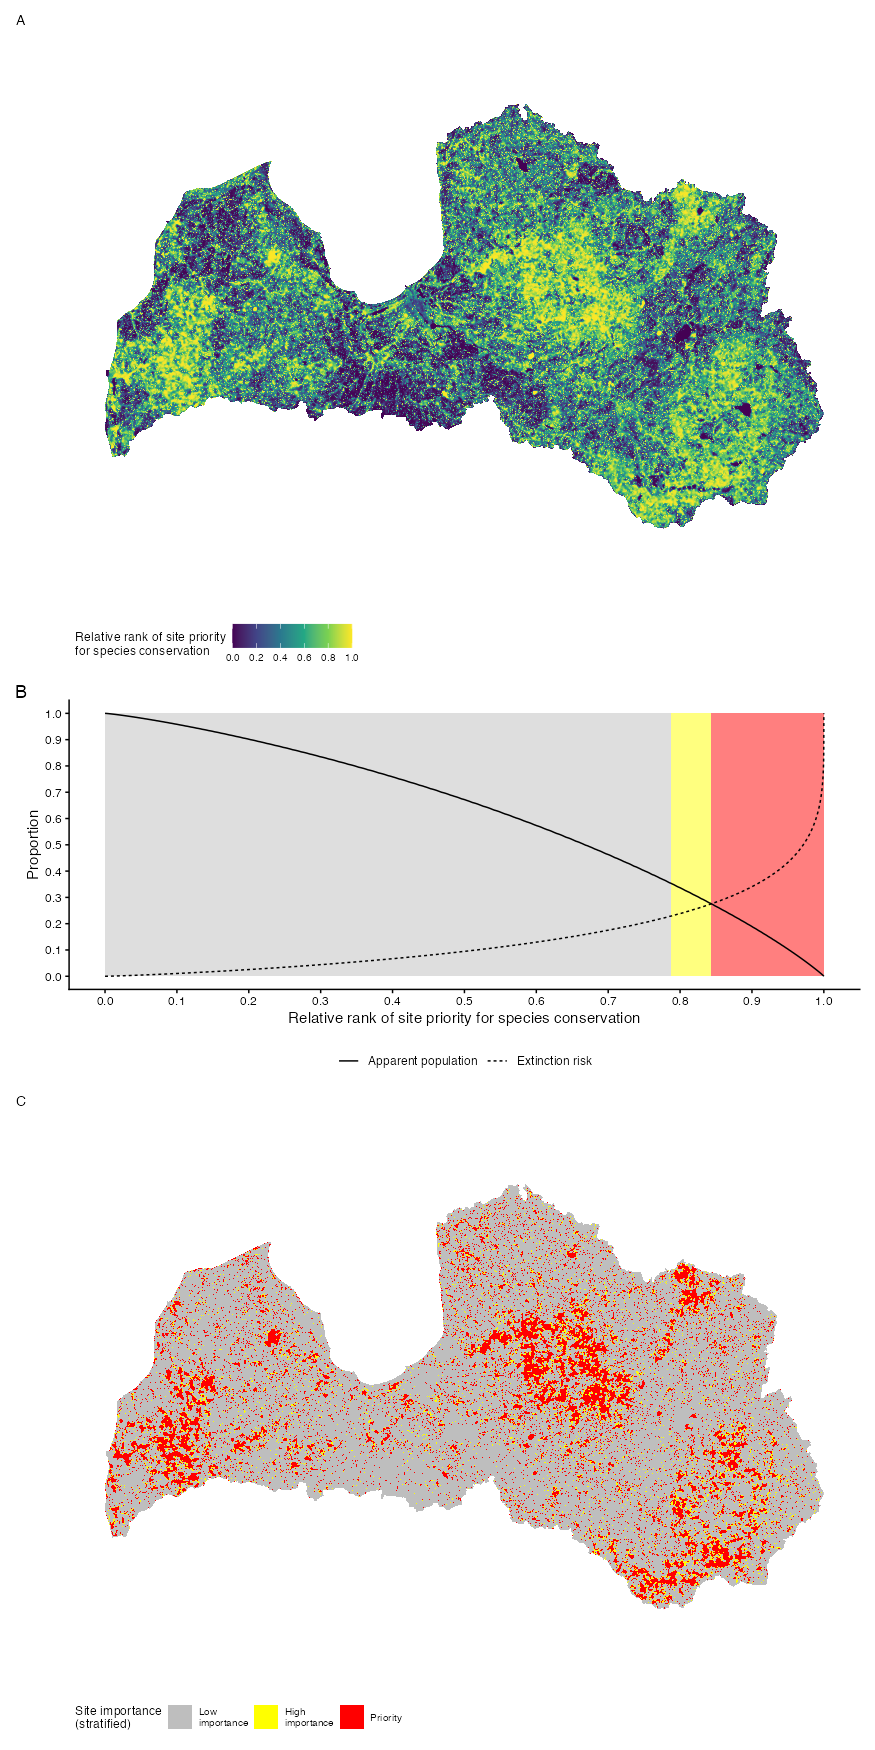
\includegraphics[width=0.85\linewidth,height=0.70\textheight,keepaspectratio]{results/LISVULlarvaev4a1/PicPrior_LISVULlarvae.png}

\par\small\textit{Single-species conservation prioritization focusing on maximisation of core area protection (CAZMAX) while accounting for site connectivity: (A) relative site rank; (B) relationship between apparent-population and extinction-risk curves with a simplified classification which is spatially demonstrated in the bootom row; (C) spatial distribution of proposed classification of site prioritization results. **For a full resolution refer to repository: link or online document: link**}\normalsize
\end{center}

\chapter*{\texorpdfstring{\emph{Triturus cristatus}}{Triturus cristatus}}\label{tricri}
\addcontentsline{toc}{chapter}{\emph{Triturus cristatus}}

\section*{Summary}\label{summary-3}
\addcontentsline{toc}{section}{Summary}

\subsection*{Model description}\label{model-description-3}
\addcontentsline{toc}{subsection}{Model description}

Occurrence and background data were divided into model-training with four block spatial cross-validation data and an independent test set. Sampling-bias/background treatment: \textbf{Phenology Weighted Target Group}. Observations were retained only where accumulated LULC change within the 1-ha analysis cell from the year of observation to 2024 did not exceed 50\%; observations were retained only where accumulated LULC change within the home-range radius around the analysis cell from the year of observation to 2024 did not exceed 50\%.

The final data set contained \textbf{162} presence records: \textbf{122} for training with four spatial block cross-validation and \textbf{40} for independent testing. Training background contained \textbf{30127} locations, with \textbf{9873} additional independent-test background locations.

\subsection*{Expert assessment scores}\label{expert-assessment-scores-3}
\addcontentsline{toc}{subsection}{Expert assessment scores}

\begin{itemize}
\tightlist
\item
  \textbf{Marginal responses and variable importance score:} 3 (moderate ecological interpretability)
\item
  \textbf{Map score:} 2 (limited agreement with known distribution)
\item
  \textbf{Applicability score:} 1 (very limited applicability)
\end{itemize}

\textbf{Šo sadaļu aizpildām manuāli no ekspertu aptaujām}

\subsection*{Statistical evaluation}\label{statistical-evaluation-3}
\addcontentsline{toc}{subsection}{Statistical evaluation}

The final model had a training TSS of \textbf{0.401}, with a training-derived cloglog threshold of \textbf{0.507}. Combined training AUC was \textbf{0.797} and combined test AUC was \textbf{0.78}.

\subsubsection*{Spatial cross-validation}\label{spatial-cross-validation-3}
\addcontentsline{toc}{subsubsection}{Spatial cross-validation}

\begin{itemize}
\tightlist
\item
  \textbf{AUC:} 0.7812 ± 0.0512; null models: 0.5327 ± 0.0367; z = 6.7668, p \textless{} 0.001
\item
  \textbf{CBI:} 0.8423 ± 0.0734; null models: 0.1371 ± 0.168; z = 4.1981, p \textless{} 0.001
\item
  \textbf{OR10:} 0.1218 ± 0.0991; null models: 0.1453 ± 0.0837; z = -0.2812, p = 0.389
\item
  \textbf{ORmin:} 0.0081 ± 0.0161; null models: 0.0209 ± 0.042; z = -0.3044, p = 0.38
\end{itemize}

\subsubsection*{Independent testing}\label{independent-testing-3}
\addcontentsline{toc}{subsubsection}{Independent testing}

\begin{itemize}
\tightlist
\item
  \textbf{TSS:} 0.462; \textbf{sensitivity:} 0.8; \textbf{specificity:} 0.662
\item
  \textbf{AUC:} 0.792; null models: 0.4791 ± 0.1084; z = 2.8861, p = 0.002
\item
  \textbf{CBI:} 0.899; null models: -0.0833 ± 0.5463; z = 1.7981, p = 0.036
\item
  \textbf{OR10:} 0.15; null models: 0.1518 ± 0.1081; z = -0.0162, p = 0.494
\item
  \textbf{ORmin:} 0.025; null models: 0.0108 ± 0.0285; z = 0.5003, p = 0.692
\end{itemize}

\subsection*{Conservation prioritisation summary}\label{conservation-prioritisation-summary-3}
\addcontentsline{toc}{subsection}{Conservation prioritisation summary}

The primary priority area covers \textbf{10.8\%} of Latvia and contains \textbf{27.6\%} of the summed habitat suitability (apparent population proxy).

The broader high importance area covers \textbf{18.7\%} of Latvia and contains \textbf{42.1\%} of the summed habitat suitability.

For comparison, the area classified as suitable using the maximum training sensitivity plus specificity habitat-suitability threshold contains \textbf{42.1\%} of the summed continuous habitat suitability.

\subsection*{Version evolution}\label{version-evolution-3}
\addcontentsline{toc}{subsection}{Version evolution}

\textbf{Šo sadaļu aizpildām manuāli, izmntojot sagatavotās shēmas. Jāvienojas par to noformējumu}

\section*{Habitat suitability}\label{habitat-suitability-3}
\addcontentsline{toc}{section}{Habitat suitability}

\begin{center}
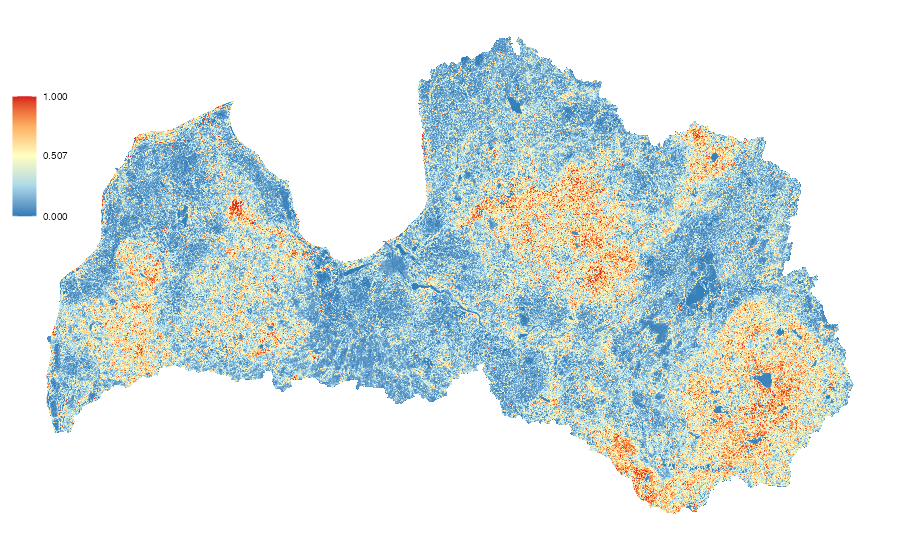
\includegraphics[width=1\linewidth,height=0.70\textheight,keepaspectratio]{results/TRICRIv4a5/PicHSmap_TRICRI.png}

\par\small\textit{Predicted continuous habitat suitability across Latvia. The warmer the colour the higher is the predicted habitat suitability. Value in the middle of the legend correspond to the maximum training sensitivity plus specificity threshold. **For a full resolution refer to repository: link or online document: link**}\normalsize
\end{center}

\section*{Model thresholds}\label{model-thresholds-3}
\addcontentsline{toc}{section}{Model thresholds}

Threshold values and associated omission rates

\begin{center}
\resizebox{\linewidth}{!}{%

\begin{tabular}{lrrrrr}
\toprule
Threshold & Cloglog value & Fractional predicted area & Training omission rate & Test omission rate & P-values\\
\midrule
Minimum training presence & 0.1135410 & 0.8712267 & 0.0000000 & 0.0001008 & 0\\
Equal training sensitivity and specificity & 0.5444789 & 0.2786771 & 0.2786885 & 0.0010078 & 0\\
Maximum training sensitivity plus specificity & 0.5069864 & 0.3184834 & 0.2295082 & 0.0008062 & 0\\
Equal test sensitivity and specificity & 0.5690751 & 0.2532343 & 0.3032787 & 0.0011085 & 0\\
Maximum test sensitivity plus specificity & 0.5249229 & 0.2992769 & 0.2622951 & 0.0008062 & 0\\
\bottomrule
\end{tabular}
}
\end{center}

\section*{Variable importance}\label{variable-importance-3}
\addcontentsline{toc}{section}{Variable importance}

\begin{center}
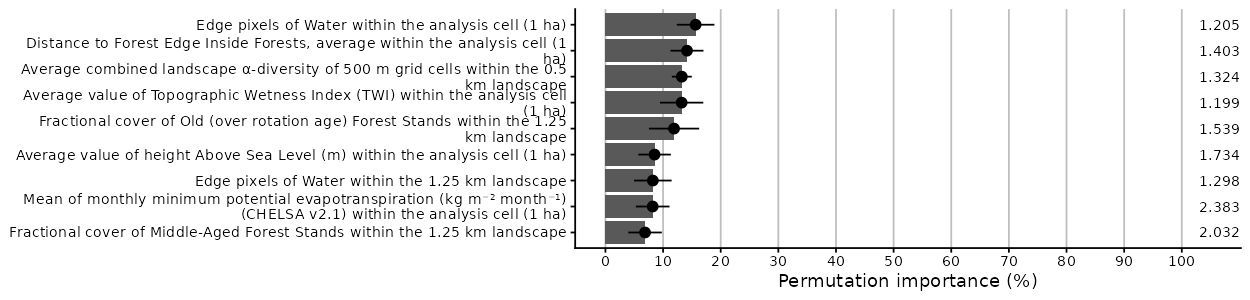
\includegraphics[width=1\linewidth,height=0.70\textheight,keepaspectratio]{results/TRICRIv4a5/PicVarImpVIFs_TRICRI.png}

\par\small\textit{Permutation-importance (mean and standard deviation from 99 permutations, on the x-axis) of the ecogeographical variables (first y-axis, left side), and their variance inflation factor values (second y-axis, right side). **For a full resolution refer to repository: link or online document: link**}\normalsize
\end{center}

\section*{Marginal responses}\label{marginal-responses-3}
\addcontentsline{toc}{section}{Marginal responses}

\begin{center}
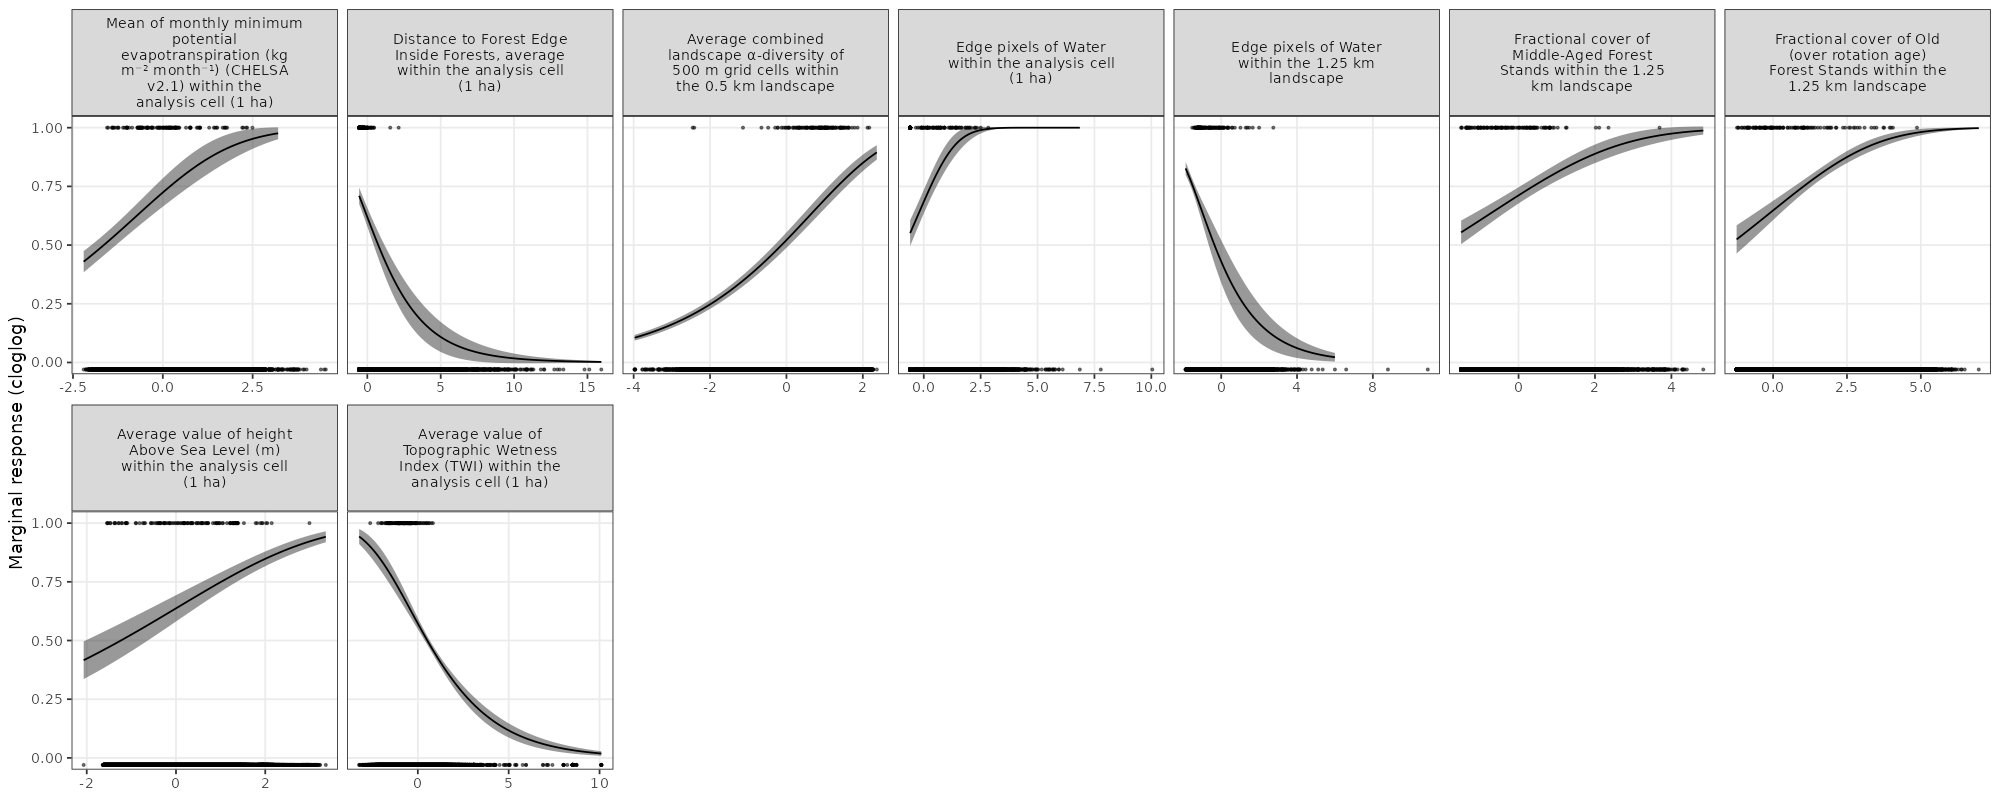
\includegraphics[width=1\linewidth,height=0.70\textheight,keepaspectratio]{results/TRICRIv4a5/PicMargResp_TRICRI.png}

\par\small\textit{Marginalised for arithmetic mean response curves illustrating the effect of each ecogeographical variable on the habitat suitability when all the other variables have their arithmetic mean values. The y-axis shows the predicted habitat suitability (cloglog-transformed), while the x-axis shows the standardised (centred and scaled) value of the ecogeographical variable. Dots at a value of 1 on the y-axis illustrate presence locations in the environment (on the x-axis), while dots at a value of 0 illustrate background locations used in modelling.  **For a full resolution refer to repository: link or online document: link**}\normalsize
\end{center}

\section*{Habitat and conservation associations}\label{habitat-and-conservation-associations-3}
\addcontentsline{toc}{section}{Habitat and conservation associations}

\begin{center}
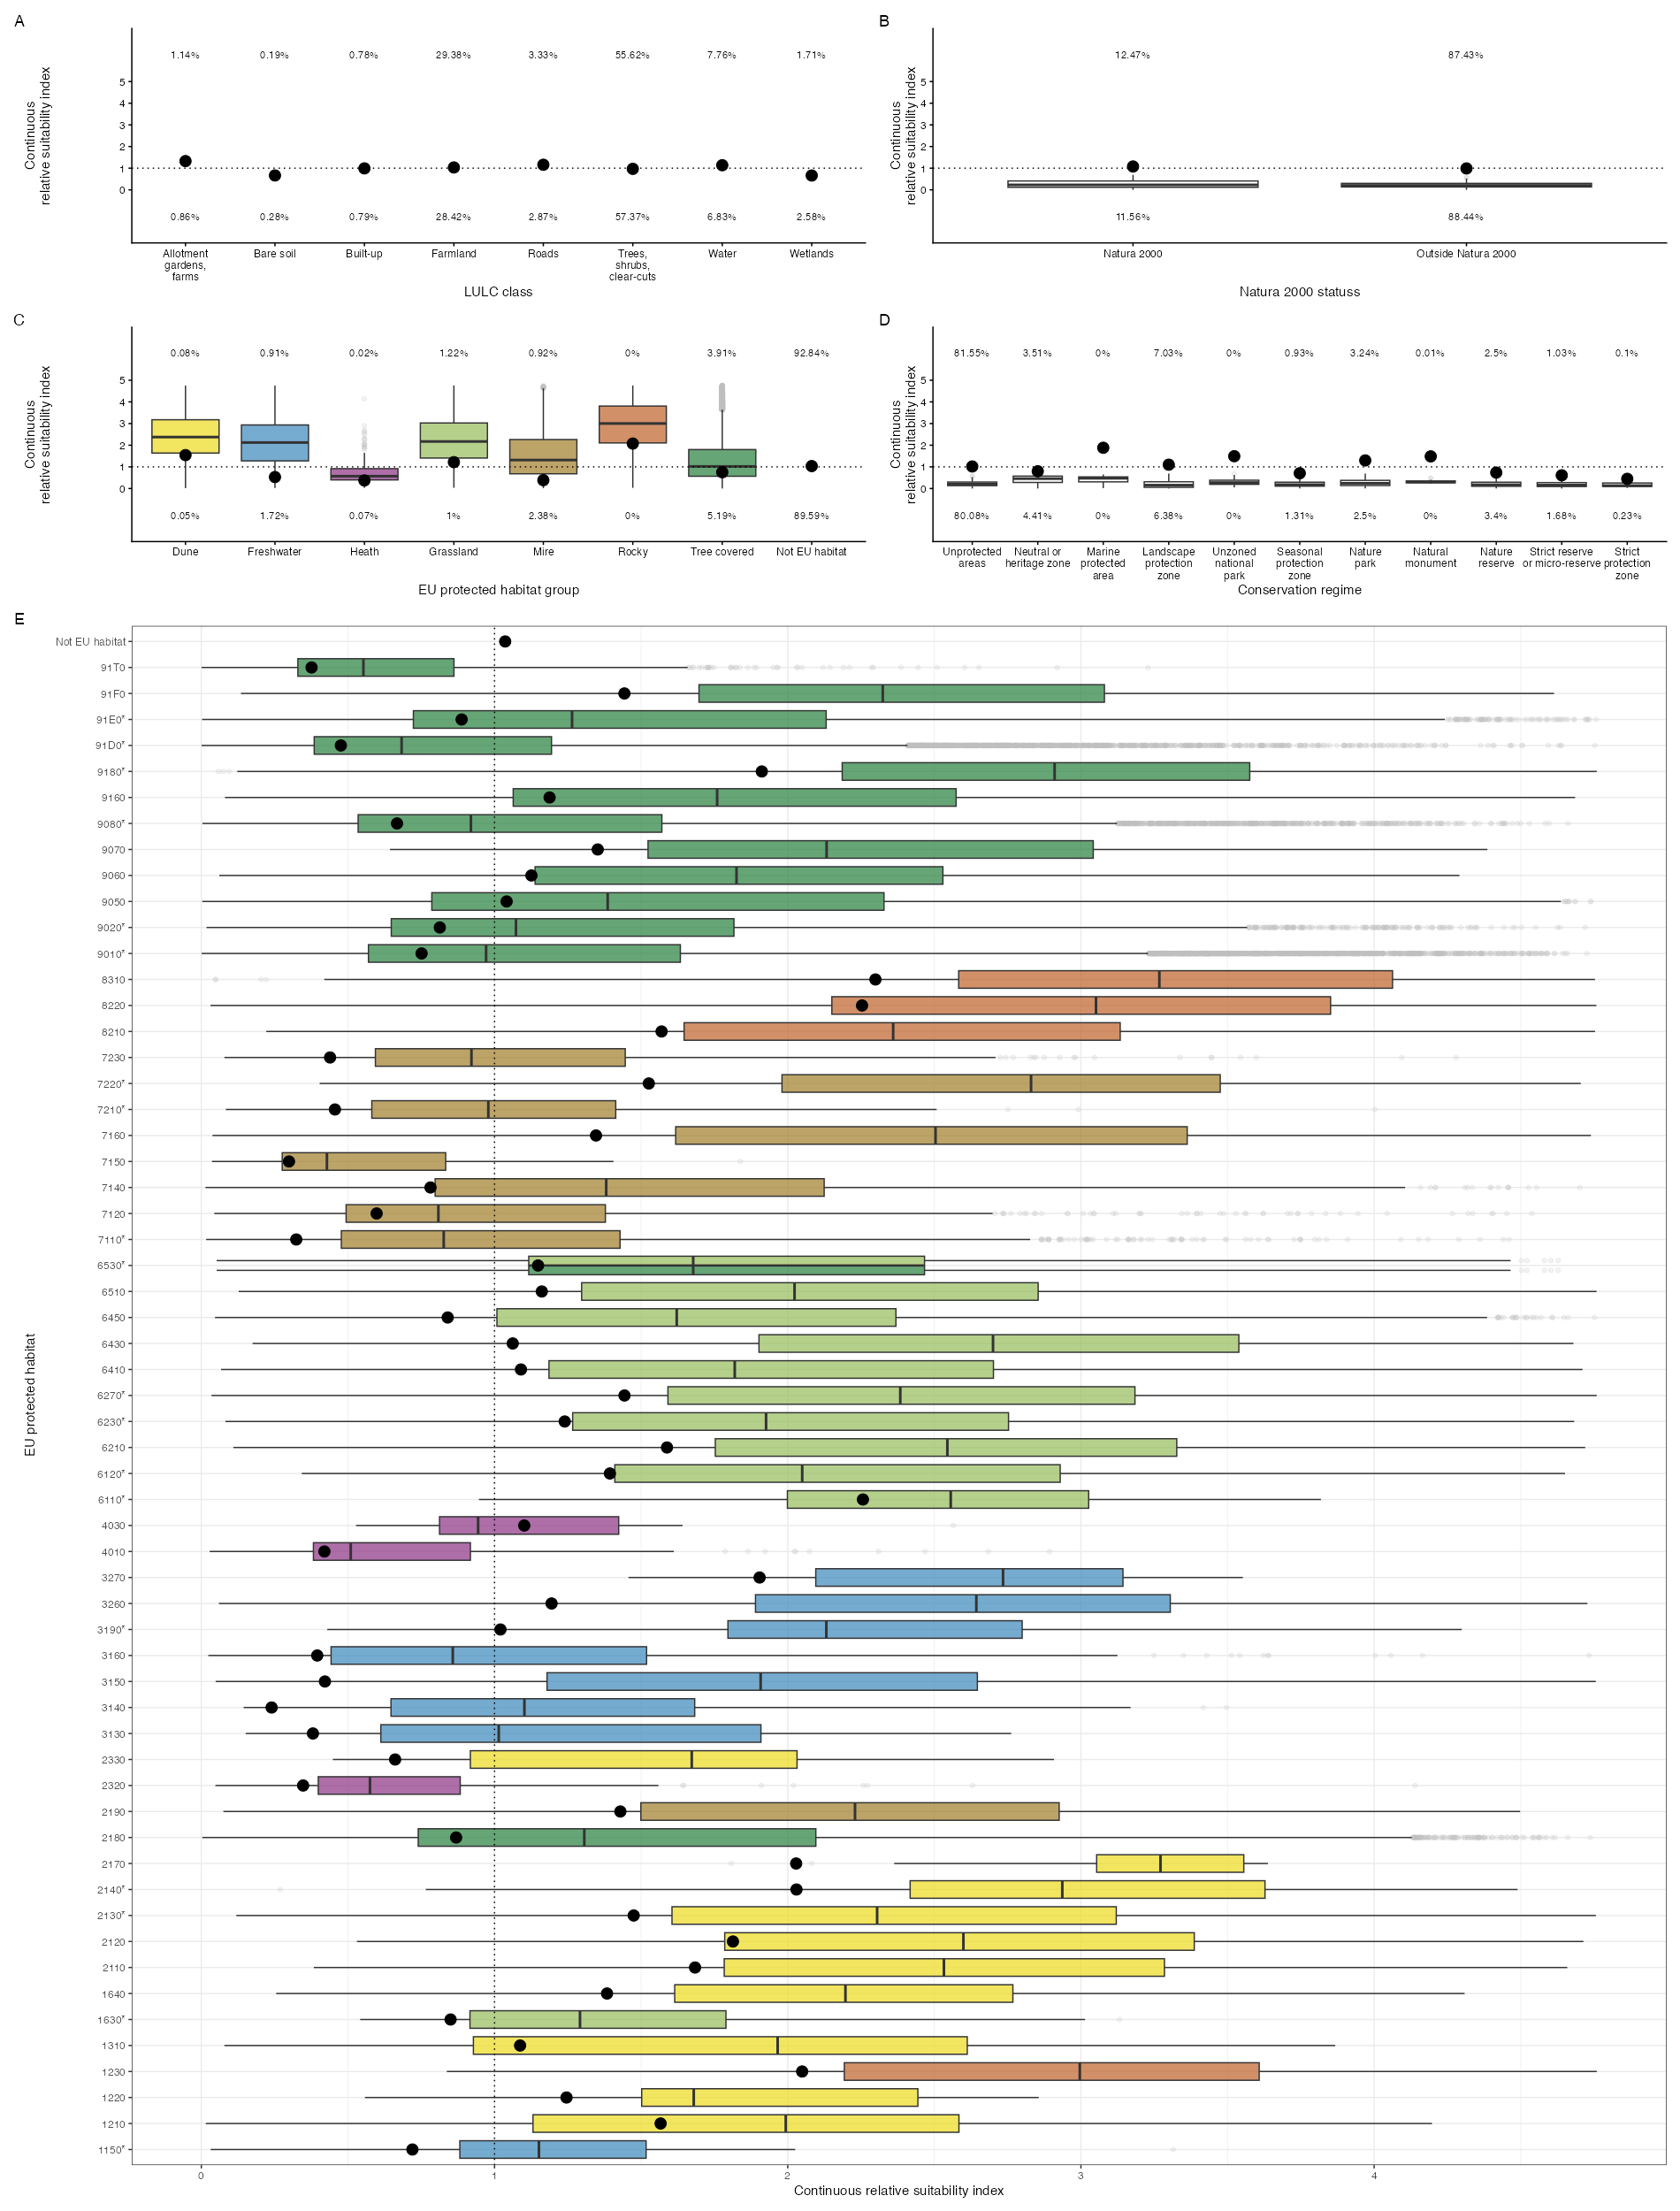
\includegraphics[width=1\linewidth,height=0.70\textheight,keepaspectratio]{results/TRICRIv4a5/PicAssoc_TRICRI.png}

\par\small\textit{Associations between predicted suitability and: (A) land use land cover classes, (B) Natura 2000 status, (C) stratified EU protected habitat classes, (D) conservation regime, and (E) EU protected habitats. The y-axis show continuous relative suitability index (derivative of Manly's index of preference). Colours in (C) and (E) correspond to stratified EU protected habitat classes. For classifications composed of multiple individual polygons, polygon-level indices were additionally calculated to show within-category variation. The figures therefore combine category-level estimates (points) with the distributions of polygon-level values (boxplots, where applicable). Labels above and below the panels report, respectively, the percentage of total predicted suitability and the percentage of mapped area represented by each category. **For a full resolution refer to repository: link or online document: link**}\normalsize
\end{center}

\section*{Conservation prioritization}\label{conservation-prioritization-3}
\addcontentsline{toc}{section}{Conservation prioritization}

\begin{center}
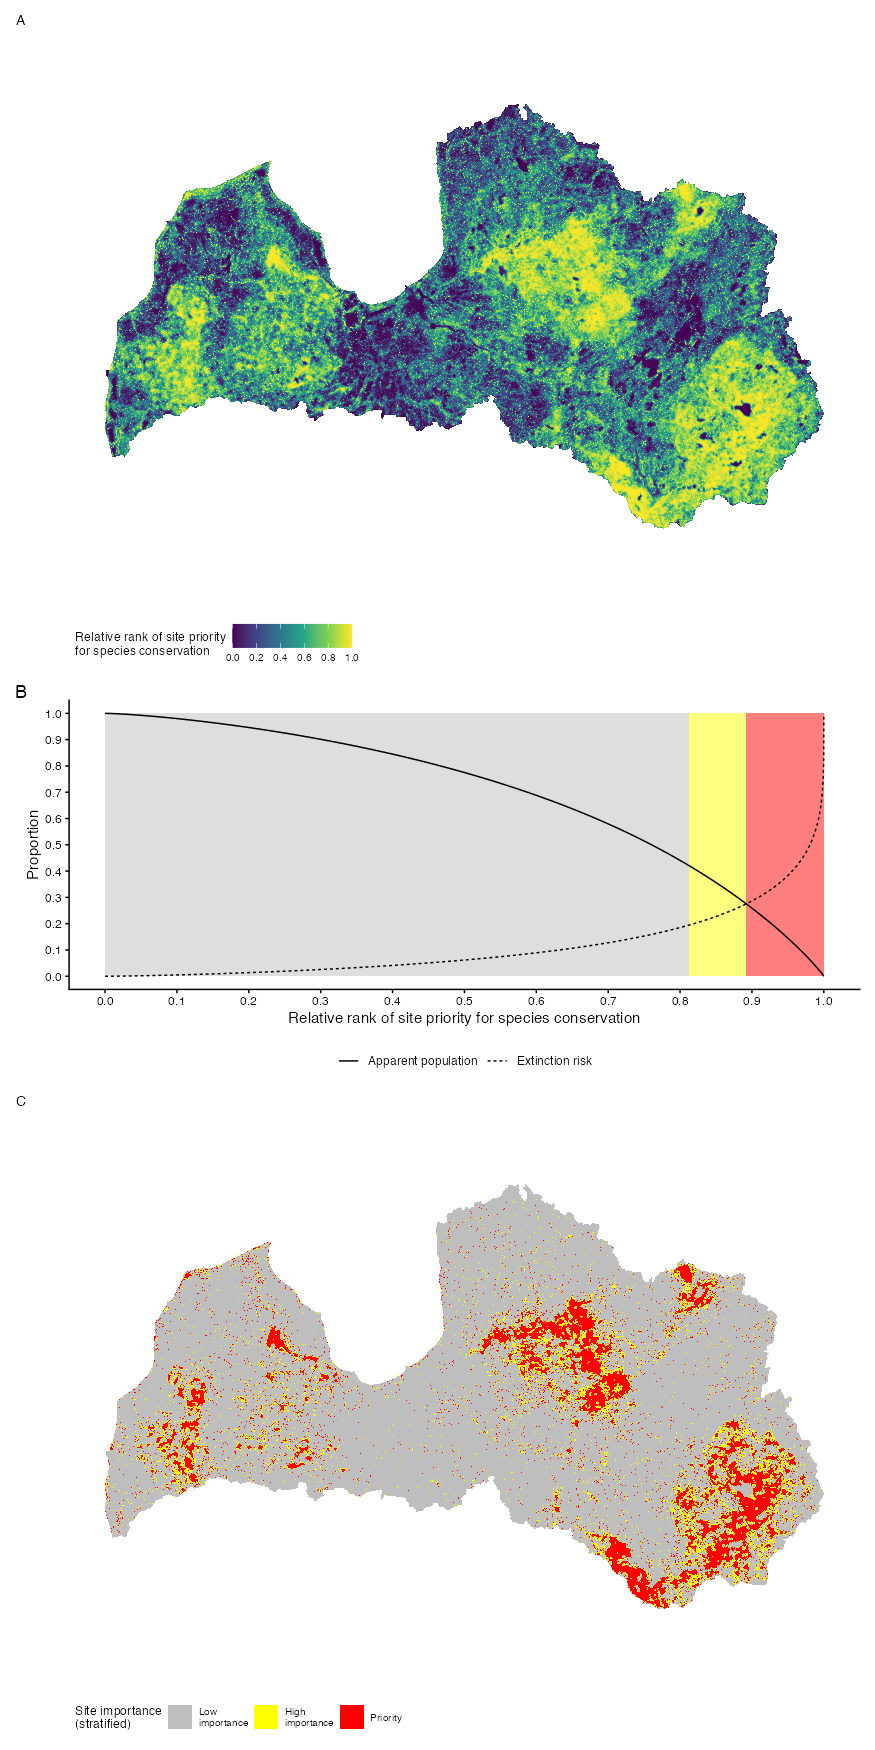
\includegraphics[width=0.85\linewidth,height=0.70\textheight,keepaspectratio]{results/TRICRIv4a5/PicPrior_TRICRI.png}

\par\small\textit{Single-species conservation prioritization focusing on maximisation of core area protection (CAZMAX) while accounting for site connectivity: (A) relative site rank; (B) relationship between apparent-population and extinction-risk curves with a simplified classification which is spatially demonstrated in the bootom row; (C) spatial distribution of proposed classification of site prioritization results. **For a full resolution refer to repository: link or online document: link**}\normalsize
\end{center}

\chapter*{\texorpdfstring{\emph{Triturus cristatus} terrestrial}{Triturus cristatus terrestrial}}\label{tricriterrestrial}
\addcontentsline{toc}{chapter}{\emph{Triturus cristatus} terrestrial}

\section*{Summary}\label{summary-4}
\addcontentsline{toc}{section}{Summary}

\subsection*{Model description}\label{model-description-4}
\addcontentsline{toc}{subsection}{Model description}

Occurrence and background data were divided into model-training with four block spatial cross-validation data and an independent test set. Sampling-bias/background treatment: \textbf{Phenology Weighted Target Group}. Accumulated LULC change within the 1-ha analysis cell was not evaluated; accumulated LULC change within the home-range radius around the analysis cell was not evaluated.

The final data set contained \textbf{87} presence records: \textbf{65} for training with four spatial block cross-validation and \textbf{22} for independent testing. Training background contained \textbf{29896} locations, with \textbf{10104} additional independent-test background locations.

\subsection*{Expert assessment scores}\label{expert-assessment-scores-4}
\addcontentsline{toc}{subsection}{Expert assessment scores}

\begin{itemize}
\tightlist
\item
  \textbf{Marginal responses and variable importance score:} 2 (limited ecological interpretability)
\item
  \textbf{Map score:} 2 (limited agreement with known distribution)
\item
  \textbf{Applicability score:} 1 (very limited applicability)
\end{itemize}

\textbf{Šo sadaļu aizpildām manuāli no ekspertu aptaujām}

\subsection*{Statistical evaluation}\label{statistical-evaluation-4}
\addcontentsline{toc}{subsection}{Statistical evaluation}

The final model had a training TSS of \textbf{0.401}, with a training-derived cloglog threshold of \textbf{0.448}. Combined training AUC was \textbf{0.826} and combined test AUC was \textbf{0.814}.

\subsubsection*{Spatial cross-validation}\label{spatial-cross-validation-4}
\addcontentsline{toc}{subsubsection}{Spatial cross-validation}

\begin{itemize}
\tightlist
\item
  \textbf{AUC:} 0.7781 ± 0.0489; null models: 0.4963 ± 0.0379; z = 7.4325, p \textless{} 0.001
\item
  \textbf{CBI:} 0.7572 ± 0.0621; null models: -0.079 ± 0.1691; z = 4.944, p \textless{} 0.001
\item
  \textbf{OR10:} 0.1985 ± 0.1007; null models: 0.2226 ± 0.0606; z = -0.3973, p = 0.346
\item
  \textbf{ORmin:} 0.0312 ± 0.0361; null models: 0.0714 ± 0.0448; z = -0.8948, p = 0.185
\end{itemize}

\subsubsection*{Independent testing}\label{independent-testing-4}
\addcontentsline{toc}{subsubsection}{Independent testing}

\begin{itemize}
\tightlist
\item
  \textbf{TSS:} 0.454; \textbf{sensitivity:} 0.773; \textbf{specificity:} 0.681
\item
  \textbf{AUC:} 0.815; null models: 0.4693 ± 0.1306; z = 2.6514, p = 0.004
\item
  \textbf{CBI:} 0.86; null models: -0.1071 ± 0.5697; z = 1.6975, p = 0.045
\item
  \textbf{OR10:} 0.136; null models: 0.2382 ± 0.1746; z = -0.5832, p = 0.28
\item
  \textbf{ORmin:} 0.046; null models: 0.0718 ± 0.1238; z = -0.213, p = 0.416
\end{itemize}

\subsection*{Conservation prioritisation summary}\label{conservation-prioritisation-summary-4}
\addcontentsline{toc}{subsection}{Conservation prioritisation summary}

The primary priority area covers \textbf{11.1\%} of Latvia and contains \textbf{27.6\%} of the summed habitat suitability (apparent population proxy).

The broader high importance area covers \textbf{23.8\%} of Latvia and contains \textbf{48.7\%} of the summed habitat suitability.

For comparison, the area classified as suitable using the maximum training sensitivity plus specificity habitat-suitability threshold contains \textbf{48.7\%} of the summed continuous habitat suitability.

\subsection*{Version evolution}\label{version-evolution-4}
\addcontentsline{toc}{subsection}{Version evolution}

\textbf{Šo sadaļu aizpildām manuāli, izmntojot sagatavotās shēmas. Jāvienojas par to noformējumu}

\section*{Habitat suitability}\label{habitat-suitability-4}
\addcontentsline{toc}{section}{Habitat suitability}

\begin{center}
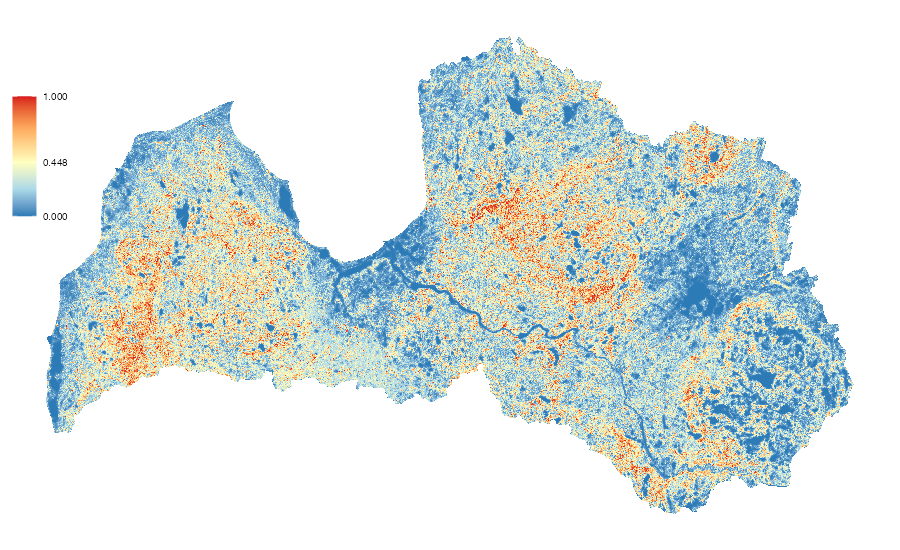
\includegraphics[width=1\linewidth,height=0.70\textheight,keepaspectratio]{results/TRICRIterrestrialv2b5/PicHSmap_TRICRIterrestrial.png}

\par\small\textit{Predicted continuous habitat suitability across Latvia. The warmer the colour the higher is the predicted habitat suitability. Value in the middle of the legend correspond to the maximum training sensitivity plus specificity threshold. **For a full resolution refer to repository: link or online document: link**}\normalsize
\end{center}

\section*{Model thresholds}\label{model-thresholds-4}
\addcontentsline{toc}{section}{Model thresholds}

Threshold values and associated omission rates

\begin{center}
\resizebox{\linewidth}{!}{%

\begin{tabular}{lrrrrr}
\toprule
Threshold & Cloglog value & Fractional predicted area & Training omission rate & Test omission rate & P-values\\
\midrule
Minimum training presence & 0.1200918 & 0.7844101 & 0.0000000 & 0.0000987 & 0\\
Equal training sensitivity and specificity & 0.4988389 & 0.2615369 & 0.2615385 & 0.0005924 & 0\\
Maximum training sensitivity plus specificity & 0.4483789 & 0.3114968 & 0.1230769 & 0.0004937 & 0\\
Equal test sensitivity and specificity & 0.4970505 & 0.2632089 & 0.2615385 & 0.0005924 & 0\\
Maximum test sensitivity plus specificity & 0.4187737 & 0.3419275 & 0.1230769 & 0.0002962 & 0\\
\bottomrule
\end{tabular}
}
\end{center}

\section*{Variable importance}\label{variable-importance-4}
\addcontentsline{toc}{section}{Variable importance}

\begin{center}
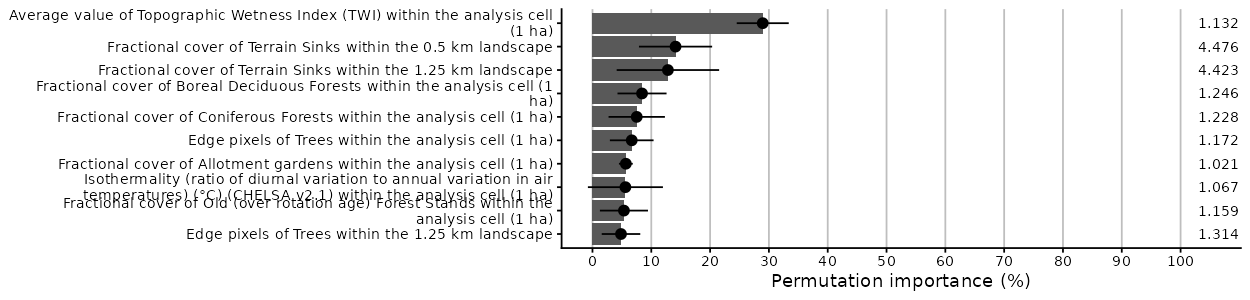
\includegraphics[width=1\linewidth,height=0.70\textheight,keepaspectratio]{results/TRICRIterrestrialv2b5/PicVarImpVIFs_TRICRIterrestrial.png}

\par\small\textit{Permutation-importance (mean and standard deviation from 99 permutations, on the x-axis) of the ecogeographical variables (first y-axis, left side), and their variance inflation factor values (second y-axis, right side). **For a full resolution refer to repository: link or online document: link**}\normalsize
\end{center}

\section*{Marginal responses}\label{marginal-responses-4}
\addcontentsline{toc}{section}{Marginal responses}

\begin{center}
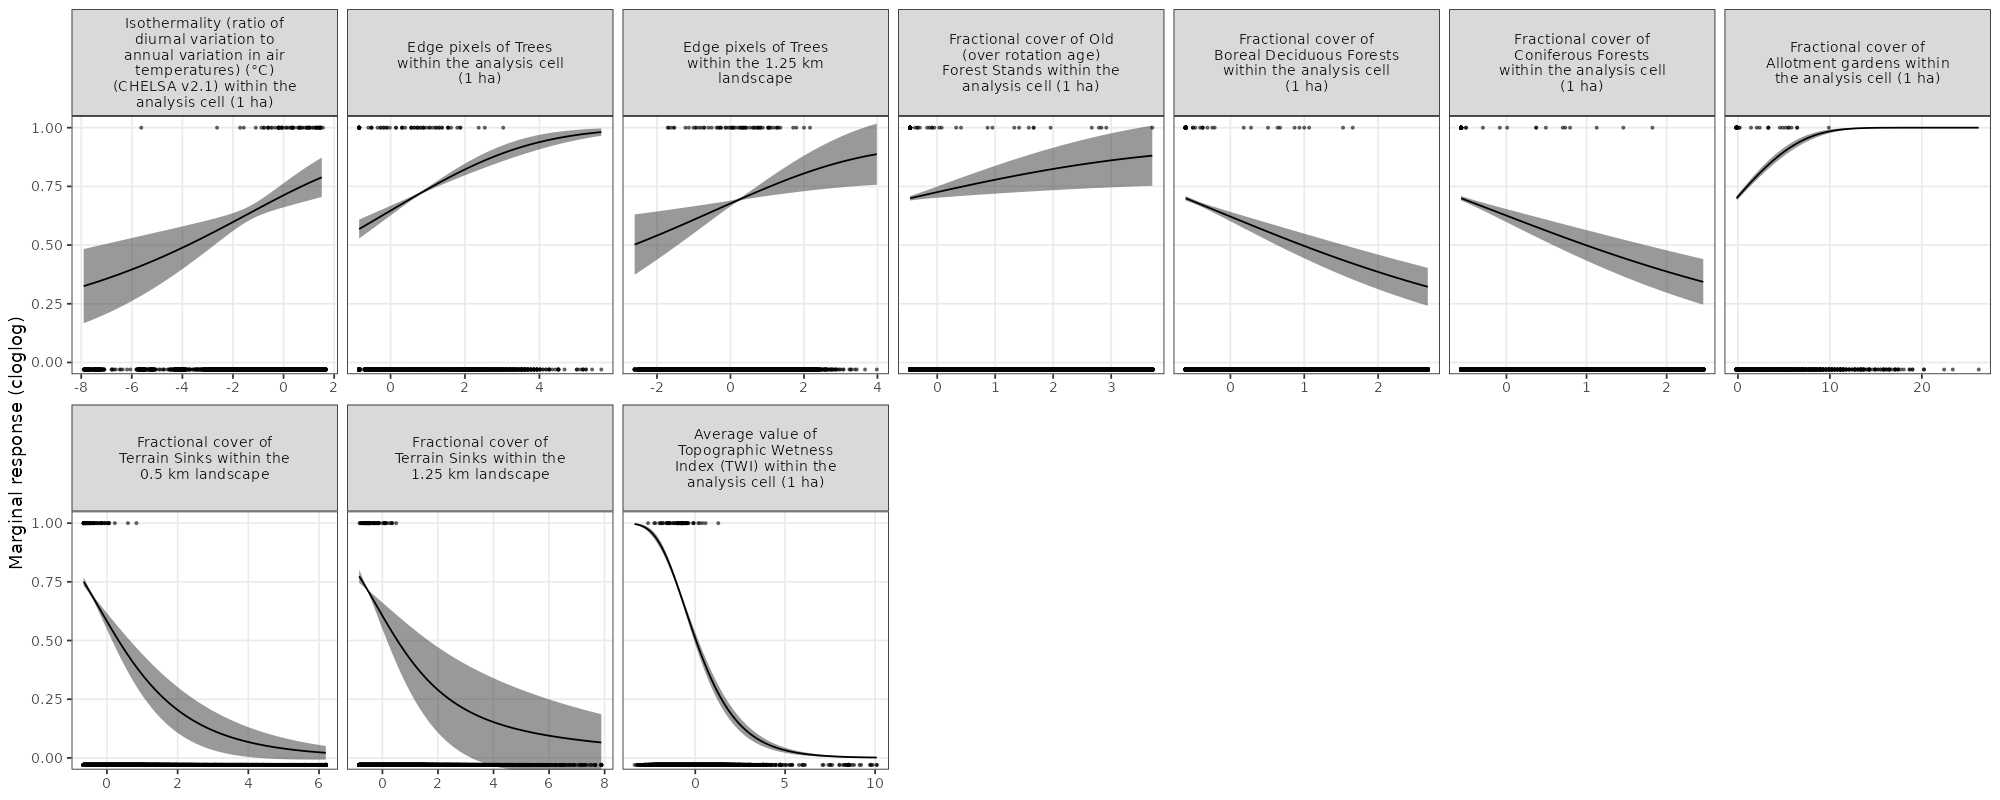
\includegraphics[width=1\linewidth,height=0.70\textheight,keepaspectratio]{results/TRICRIterrestrialv2b5/PicMargResp_TRICRIterrestrial.png}

\par\small\textit{Marginalised for arithmetic mean response curves illustrating the effect of each ecogeographical variable on the habitat suitability when all the other variables have their arithmetic mean values. The y-axis shows the predicted habitat suitability (cloglog-transformed), while the x-axis shows the standardised (centred and scaled) value of the ecogeographical variable. Dots at a value of 1 on the y-axis illustrate presence locations in the environment (on the x-axis), while dots at a value of 0 illustrate background locations used in modelling.  **For a full resolution refer to repository: link or online document: link**}\normalsize
\end{center}

\section*{Habitat and conservation associations}\label{habitat-and-conservation-associations-4}
\addcontentsline{toc}{section}{Habitat and conservation associations}

\begin{center}
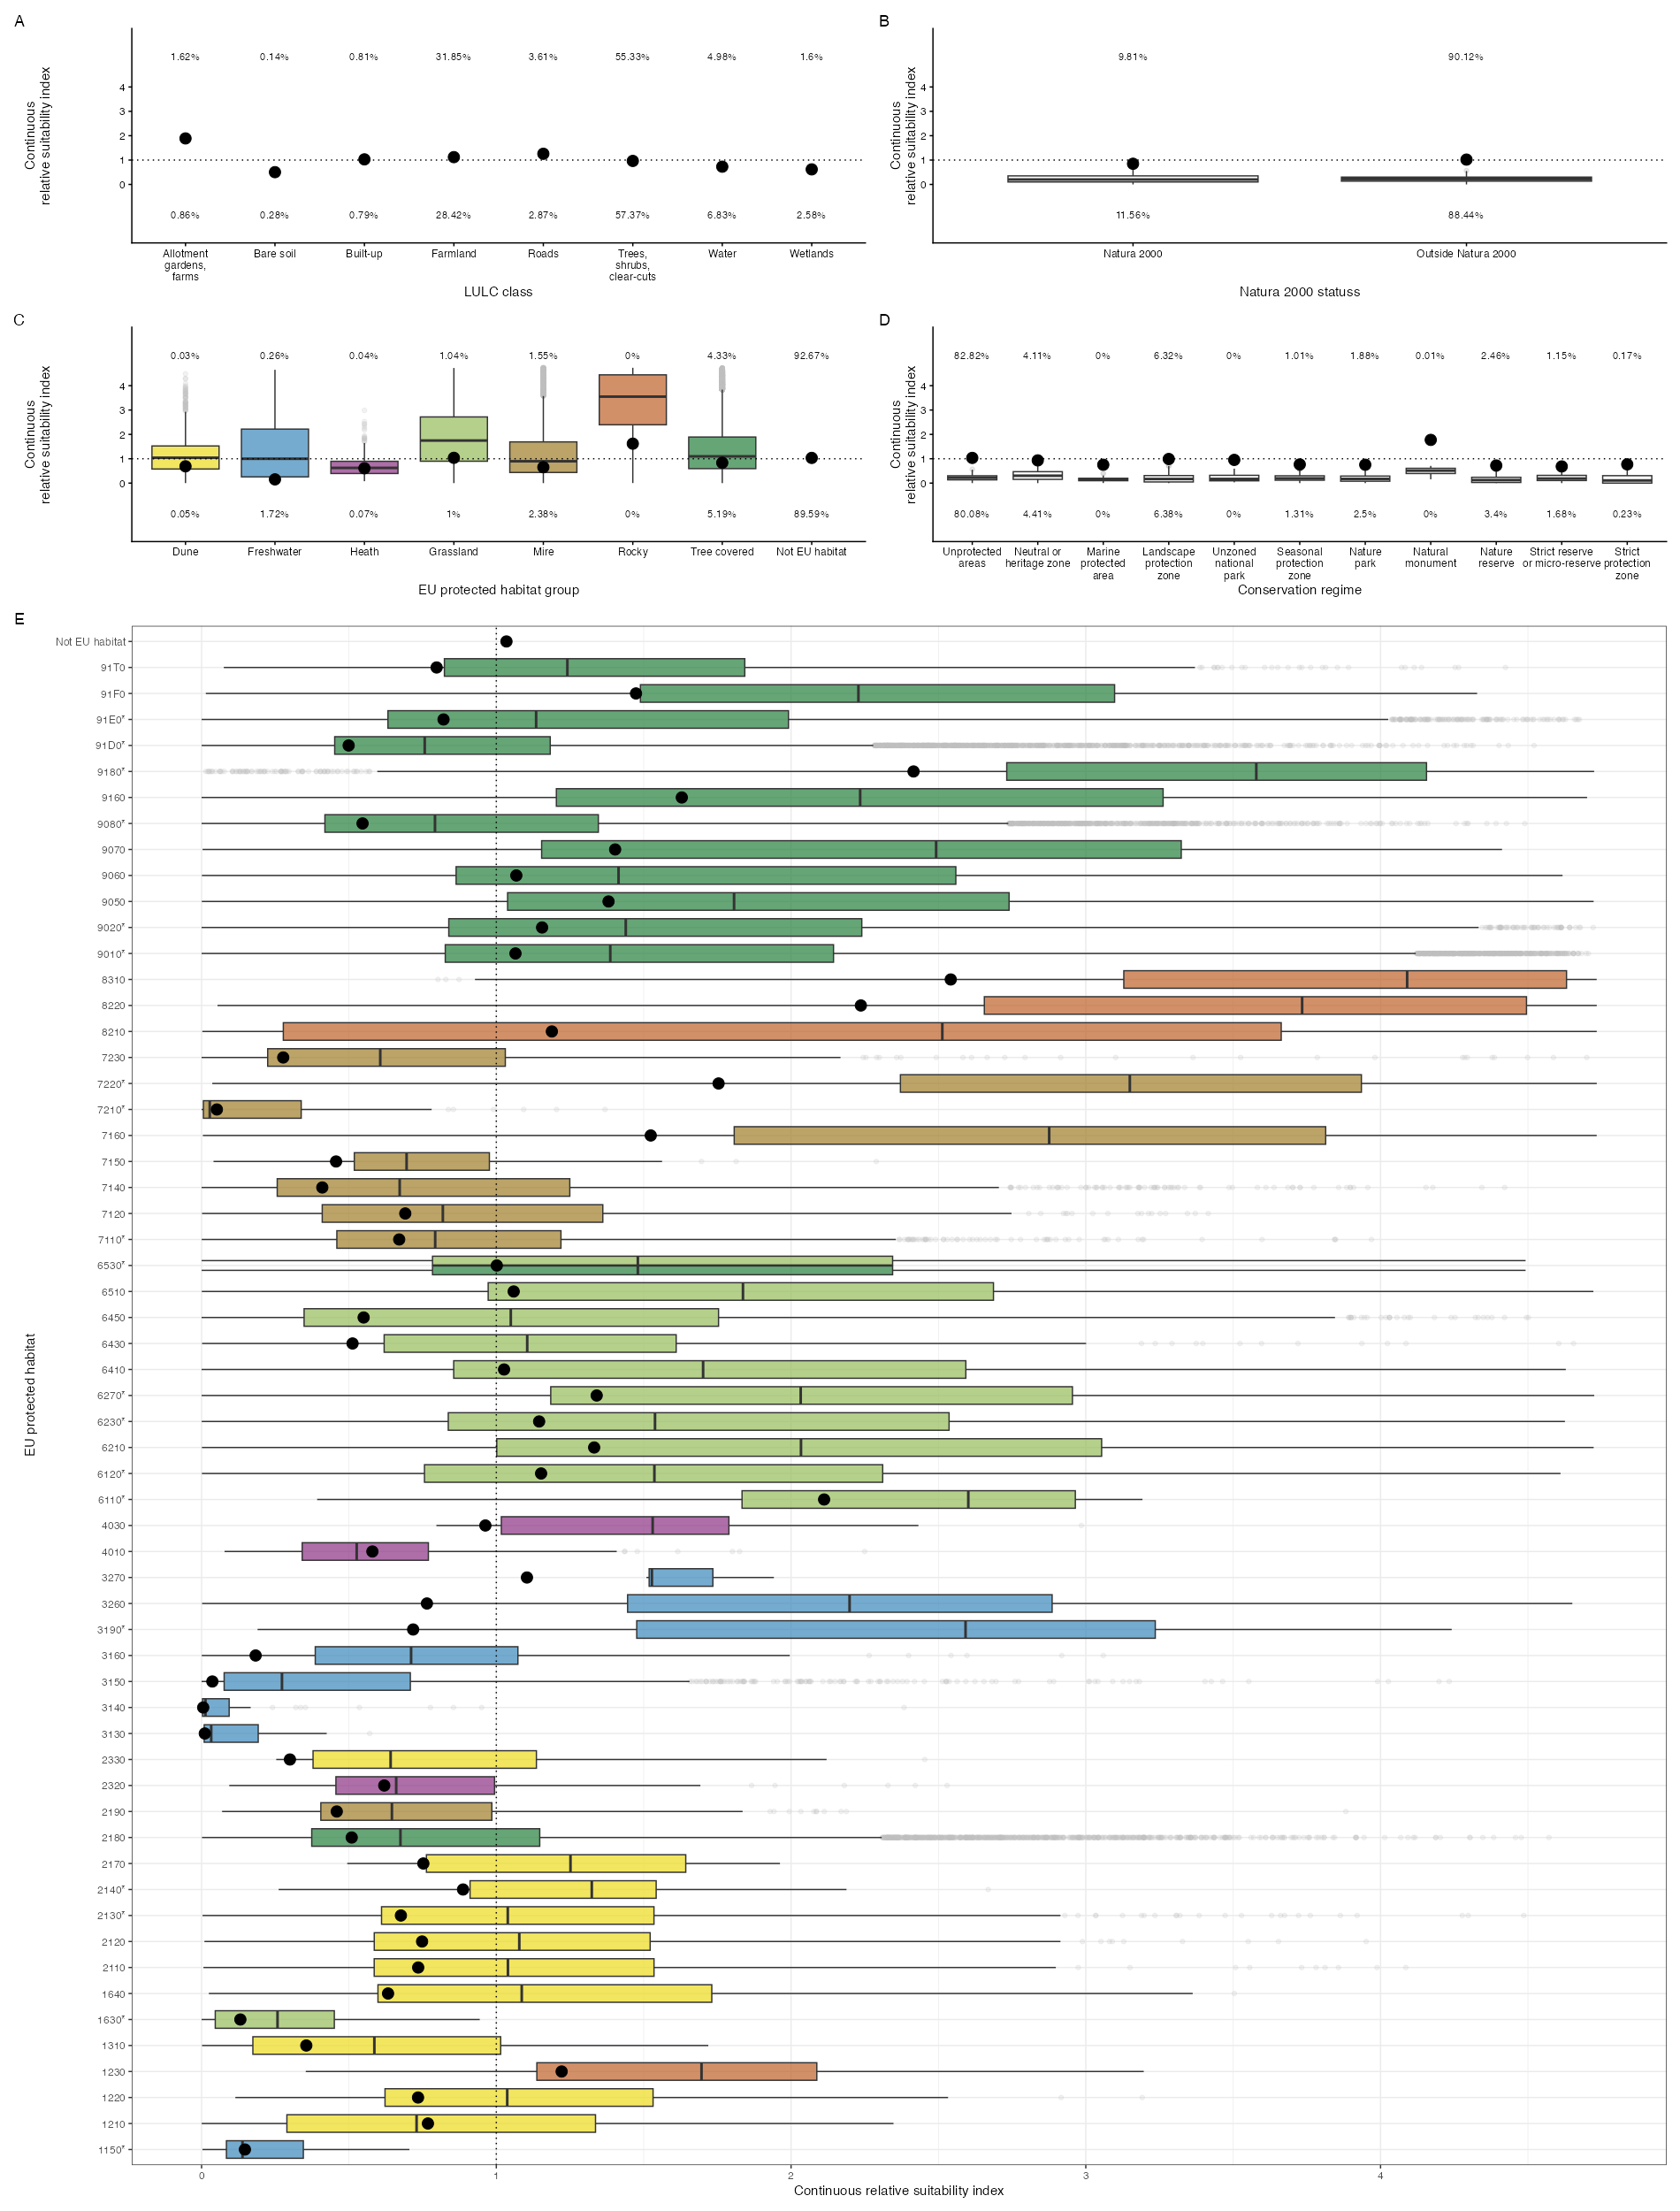
\includegraphics[width=1\linewidth,height=0.70\textheight,keepaspectratio]{results/TRICRIterrestrialv2b5/PicAssoc_TRICRIterrestrial.png}

\par\small\textit{Associations between predicted suitability and: (A) land use land cover classes, (B) Natura 2000 status, (C) stratified EU protected habitat classes, (D) conservation regime, and (E) EU protected habitats. The y-axis show continuous relative suitability index (derivative of Manly's index of preference). Colours in (C) and (E) correspond to stratified EU protected habitat classes. For classifications composed of multiple individual polygons, polygon-level indices were additionally calculated to show within-category variation. The figures therefore combine category-level estimates (points) with the distributions of polygon-level values (boxplots, where applicable). Labels above and below the panels report, respectively, the percentage of total predicted suitability and the percentage of mapped area represented by each category. **For a full resolution refer to repository: link or online document: link**}\normalsize
\end{center}

\section*{Conservation prioritization}\label{conservation-prioritization-4}
\addcontentsline{toc}{section}{Conservation prioritization}

\begin{center}
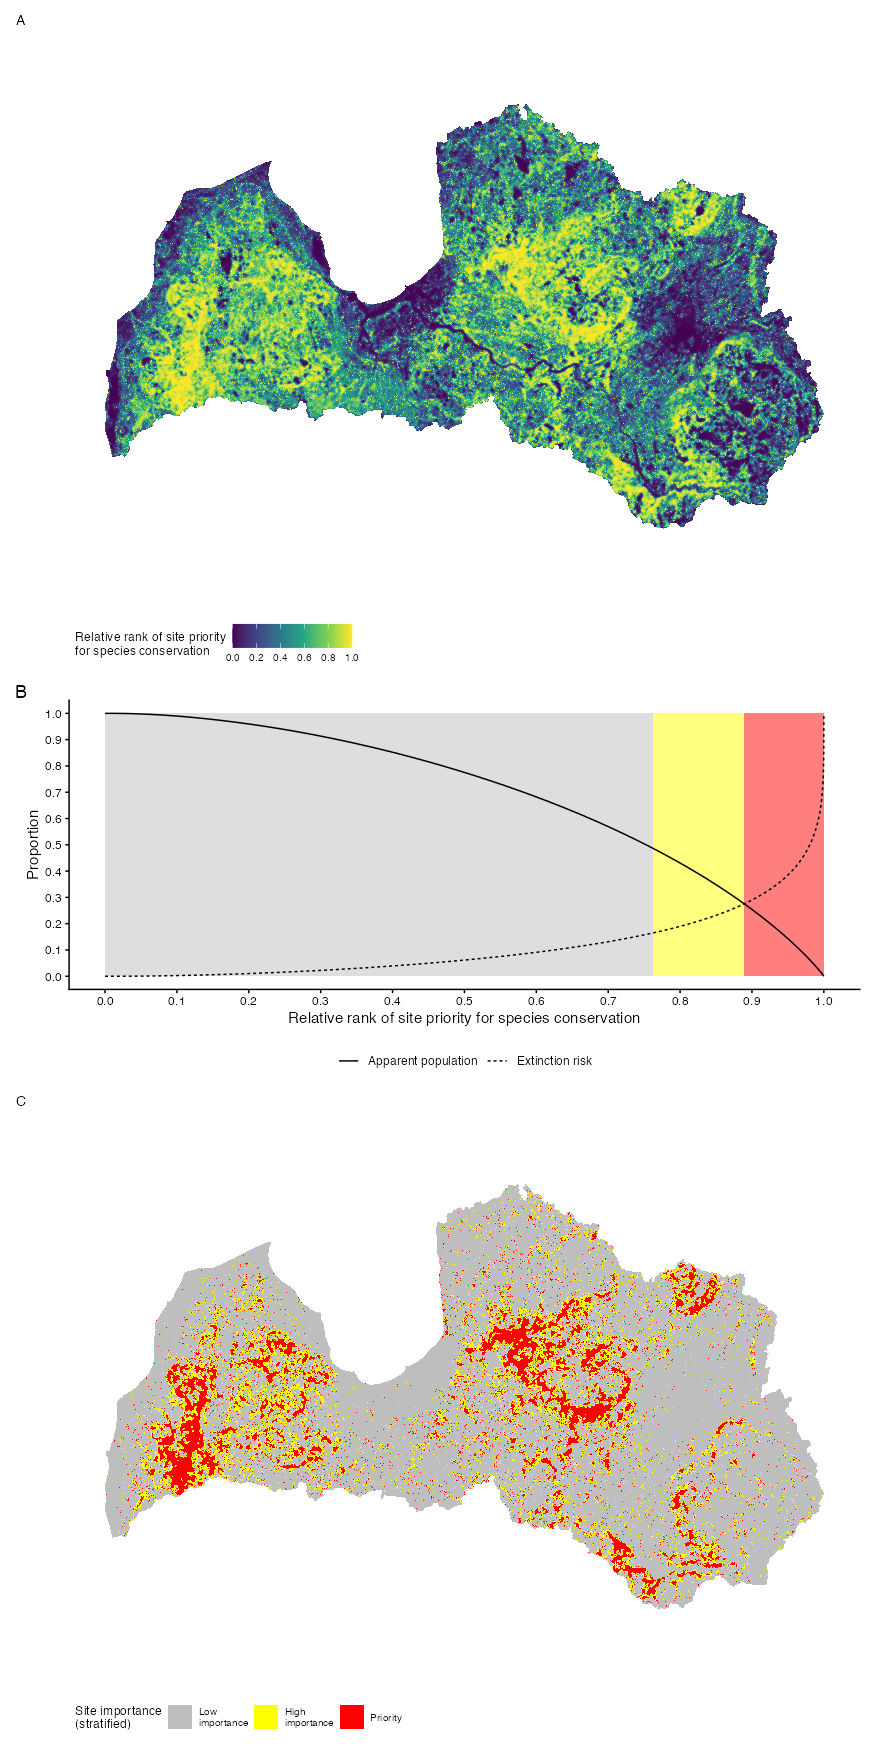
\includegraphics[width=0.85\linewidth,height=0.70\textheight,keepaspectratio]{results/TRICRIterrestrialv2b5/PicPrior_TRICRIterrestrial.png}

\par\small\textit{Single-species conservation prioritization focusing on maximisation of core area protection (CAZMAX) while accounting for site connectivity: (A) relative site rank; (B) relationship between apparent-population and extinction-risk curves with a simplified classification which is spatially demonstrated in the bootom row; (C) spatial distribution of proposed classification of site prioritization results. **For a full resolution refer to repository: link or online document: link**}\normalsize
\end{center}

\chapter*{\texorpdfstring{\emph{Triturus cristatus} larvae}{Triturus cristatus larvae}}\label{tricrilarvae}
\addcontentsline{toc}{chapter}{\emph{Triturus cristatus} larvae}

\section*{Summary}\label{summary-5}
\addcontentsline{toc}{section}{Summary}

\subsection*{Model description}\label{model-description-5}
\addcontentsline{toc}{subsection}{Model description}

Occurrence and background data were divided into model-training with four block spatial cross-validation data and an independent test set. Sampling-bias/background treatment: \textbf{Phenology Weighted Target Group}. Accumulated LULC change within the 1-ha analysis cell was not evaluated; accumulated LULC change within the home-range radius around the analysis cell was not evaluated.

The final data set contained \textbf{150} presence records: \textbf{112} for training with four spatial block cross-validation and \textbf{38} for independent testing. Training background contained \textbf{29876} locations, with \textbf{10124} additional independent-test background locations.

\subsection*{Expert assessment scores}\label{expert-assessment-scores-5}
\addcontentsline{toc}{subsection}{Expert assessment scores}

\begin{itemize}
\tightlist
\item
  \textbf{Marginal responses and variable importance score:} 4 (good ecological interpretability)
\item
  \textbf{Map score:} 3 (moderate agreement with known distribution)
\item
  \textbf{Applicability score:} 3 (moderate applicability)
\end{itemize}

\textbf{Šo sadaļu aizpildām manuāli no ekspertu aptaujām}

\subsection*{Statistical evaluation}\label{statistical-evaluation-5}
\addcontentsline{toc}{subsection}{Statistical evaluation}

The final model had a training TSS of \textbf{0.401}, with a training-derived cloglog threshold of \textbf{0.341}. Combined training AUC was \textbf{0.903} and combined test AUC was \textbf{0.861}.

\subsubsection*{Spatial cross-validation}\label{spatial-cross-validation-5}
\addcontentsline{toc}{subsubsection}{Spatial cross-validation}

\begin{itemize}
\tightlist
\item
  \textbf{AUC:} 0.8312 ± 0.0622; null models: 0.5071 ± 0.0444; z = 7.299, p \textless{} 0.001
\item
  \textbf{CBI:} 0.8105 ± 0.0671; null models: 0.0373 ± 0.1748; z = 4.4222, p \textless{} 0.001
\item
  \textbf{OR10:} 0.2232 ± 0.2376; null models: 0.2442 ± 0.096; z = -0.2186, p = 0.413
\item
  \textbf{ORmin:} 0.1607 ± 0.2551; null models: 0.0624 ± 0.1067; z = 0.9215, p = 0.822
\end{itemize}

\subsubsection*{Independent testing}\label{independent-testing-5}
\addcontentsline{toc}{subsubsection}{Independent testing}

\begin{itemize}
\tightlist
\item
  \textbf{TSS:} 0.495; \textbf{sensitivity:} 0.711; \textbf{specificity:} 0.785
\item
  \textbf{AUC:} 0.861; null models: 0.5146 ± 0.1166; z = 2.9716, p = 0.001
\item
  \textbf{CBI:} 0.881; null models: 0.0472 ± 0.5315; z = 1.5689, p = 0.058
\item
  \textbf{OR10:} 0.237; null models: 0.1926 ± 0.127; z = 0.3481, p = 0.636
\item
  \textbf{ORmin:} 0; null models: 0.0229 ± 0.0384; z = -0.5955, p = 0.276
\end{itemize}

\subsection*{Conservation prioritisation summary}\label{conservation-prioritisation-summary-5}
\addcontentsline{toc}{subsection}{Conservation prioritisation summary}

The primary priority area covers \textbf{5\%} of Latvia and contains \textbf{27.6\%} of the summed habitat suitability (apparent population proxy).

The broader high importance area covers \textbf{11\%} of Latvia and contains \textbf{44.7\%} of the summed habitat suitability.

For comparison, the area classified as suitable using the maximum training sensitivity plus specificity habitat-suitability threshold contains \textbf{44.7\%} of the summed continuous habitat suitability.

\subsection*{Version evolution}\label{version-evolution-5}
\addcontentsline{toc}{subsection}{Version evolution}

\textbf{Šo sadaļu aizpildām manuāli, izmntojot sagatavotās shēmas. Jāvienojas par to noformējumu}

\section*{Habitat suitability}\label{habitat-suitability-5}
\addcontentsline{toc}{section}{Habitat suitability}

\begin{center}
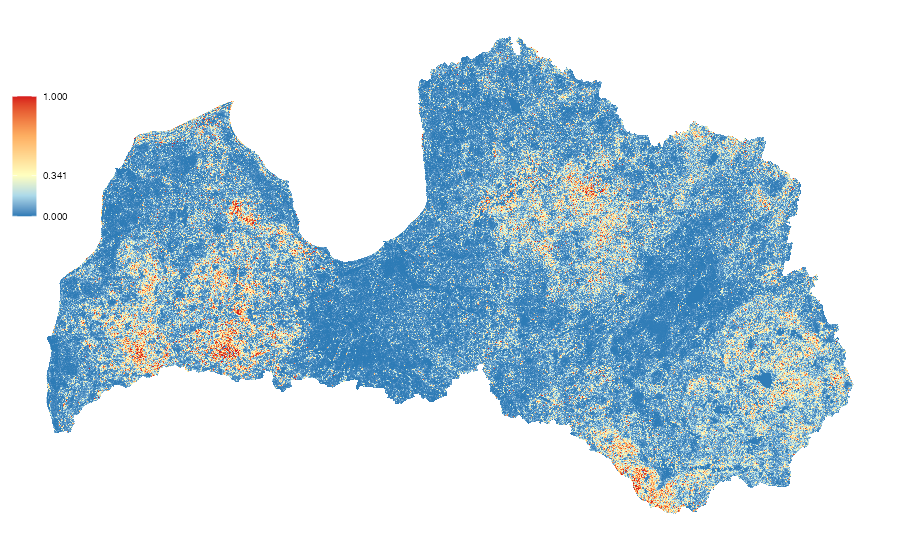
\includegraphics[width=1\linewidth,height=0.70\textheight,keepaspectratio]{results/TRICRIlarvaev2b1/PicHSmap_TRICRIlarvae.png}

\par\small\textit{Predicted continuous habitat suitability across Latvia. The warmer the colour the higher is the predicted habitat suitability. Value in the middle of the legend correspond to the maximum training sensitivity plus specificity threshold. **For a full resolution refer to repository: link or online document: link**}\normalsize
\end{center}

\section*{Model thresholds}\label{model-thresholds-5}
\addcontentsline{toc}{section}{Model thresholds}

Threshold values and associated omission rates

\begin{center}
\resizebox{\linewidth}{!}{%

\begin{tabular}{lrrrrr}
\toprule
Threshold & Cloglog value & Fractional predicted area & Training omission rate & Test omission rate & P-values\\
\midrule
Minimum training presence & 0.0397720 & 0.7029703 & 0.0000000 & 0.0000000 & 0\\
Equal training sensitivity and specificity & 0.4097315 & 0.1696548 & 0.1696429 & 0.0010811 & 0\\
Maximum training sensitivity plus specificity & 0.3409909 & 0.2134734 & 0.1160714 & 0.0010811 & 0\\
Equal test sensitivity and specificity & 0.3100209 & 0.2371889 & 0.1071429 & 0.0008845 & 0\\
Maximum test sensitivity plus specificity & 0.4586229 & 0.1440995 & 0.2053571 & 0.0010811 & 0\\
\bottomrule
\end{tabular}
}
\end{center}

\section*{Variable importance}\label{variable-importance-5}
\addcontentsline{toc}{section}{Variable importance}

\begin{center}
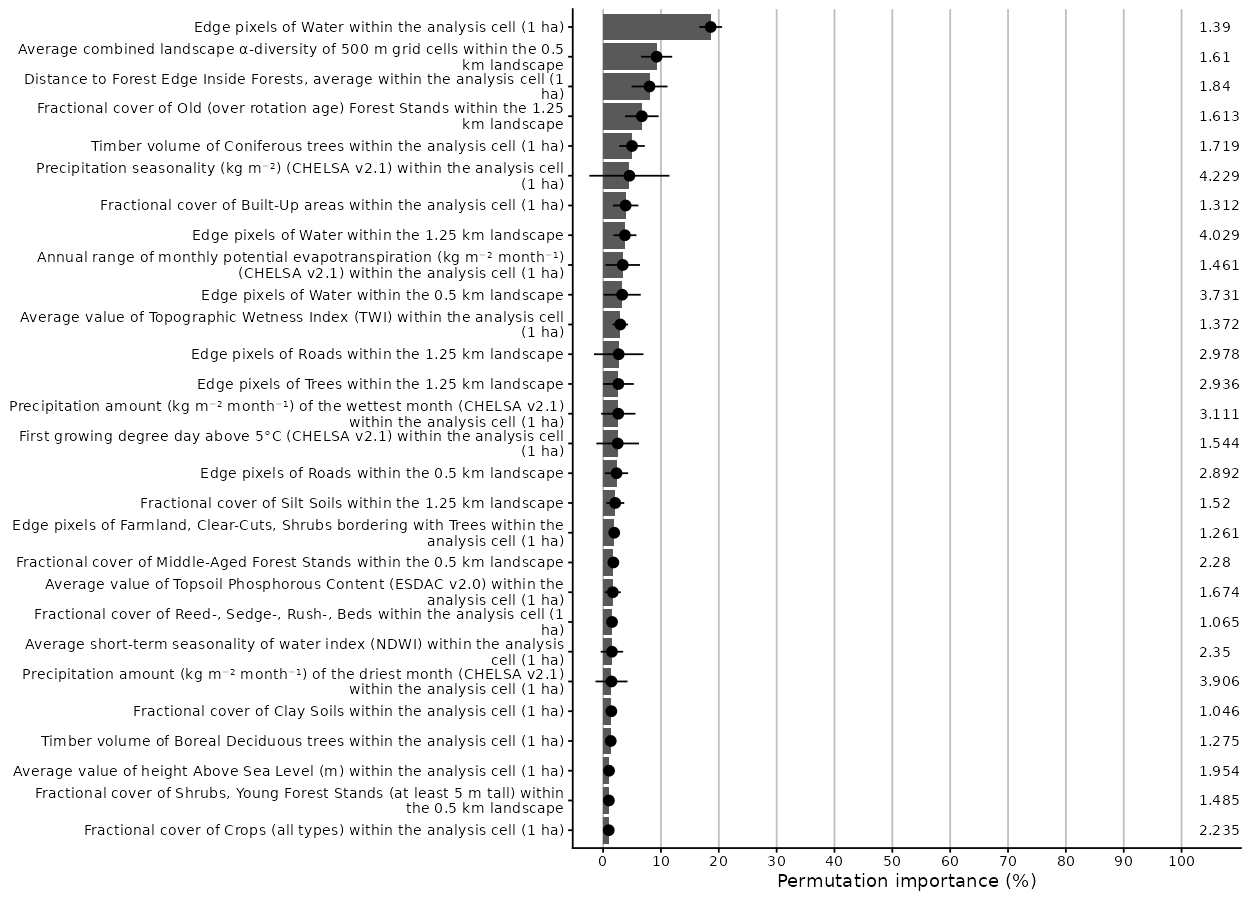
\includegraphics[width=1\linewidth,height=0.70\textheight,keepaspectratio]{results/TRICRIlarvaev2b1/PicVarImpVIFs_TRICRIlarvae.png}

\par\small\textit{Permutation-importance (mean and standard deviation from 99 permutations, on the x-axis) of the ecogeographical variables (first y-axis, left side), and their variance inflation factor values (second y-axis, right side). **For a full resolution refer to repository: link or online document: link**}\normalsize
\end{center}

\section*{Marginal responses}\label{marginal-responses-5}
\addcontentsline{toc}{section}{Marginal responses}

\begin{center}
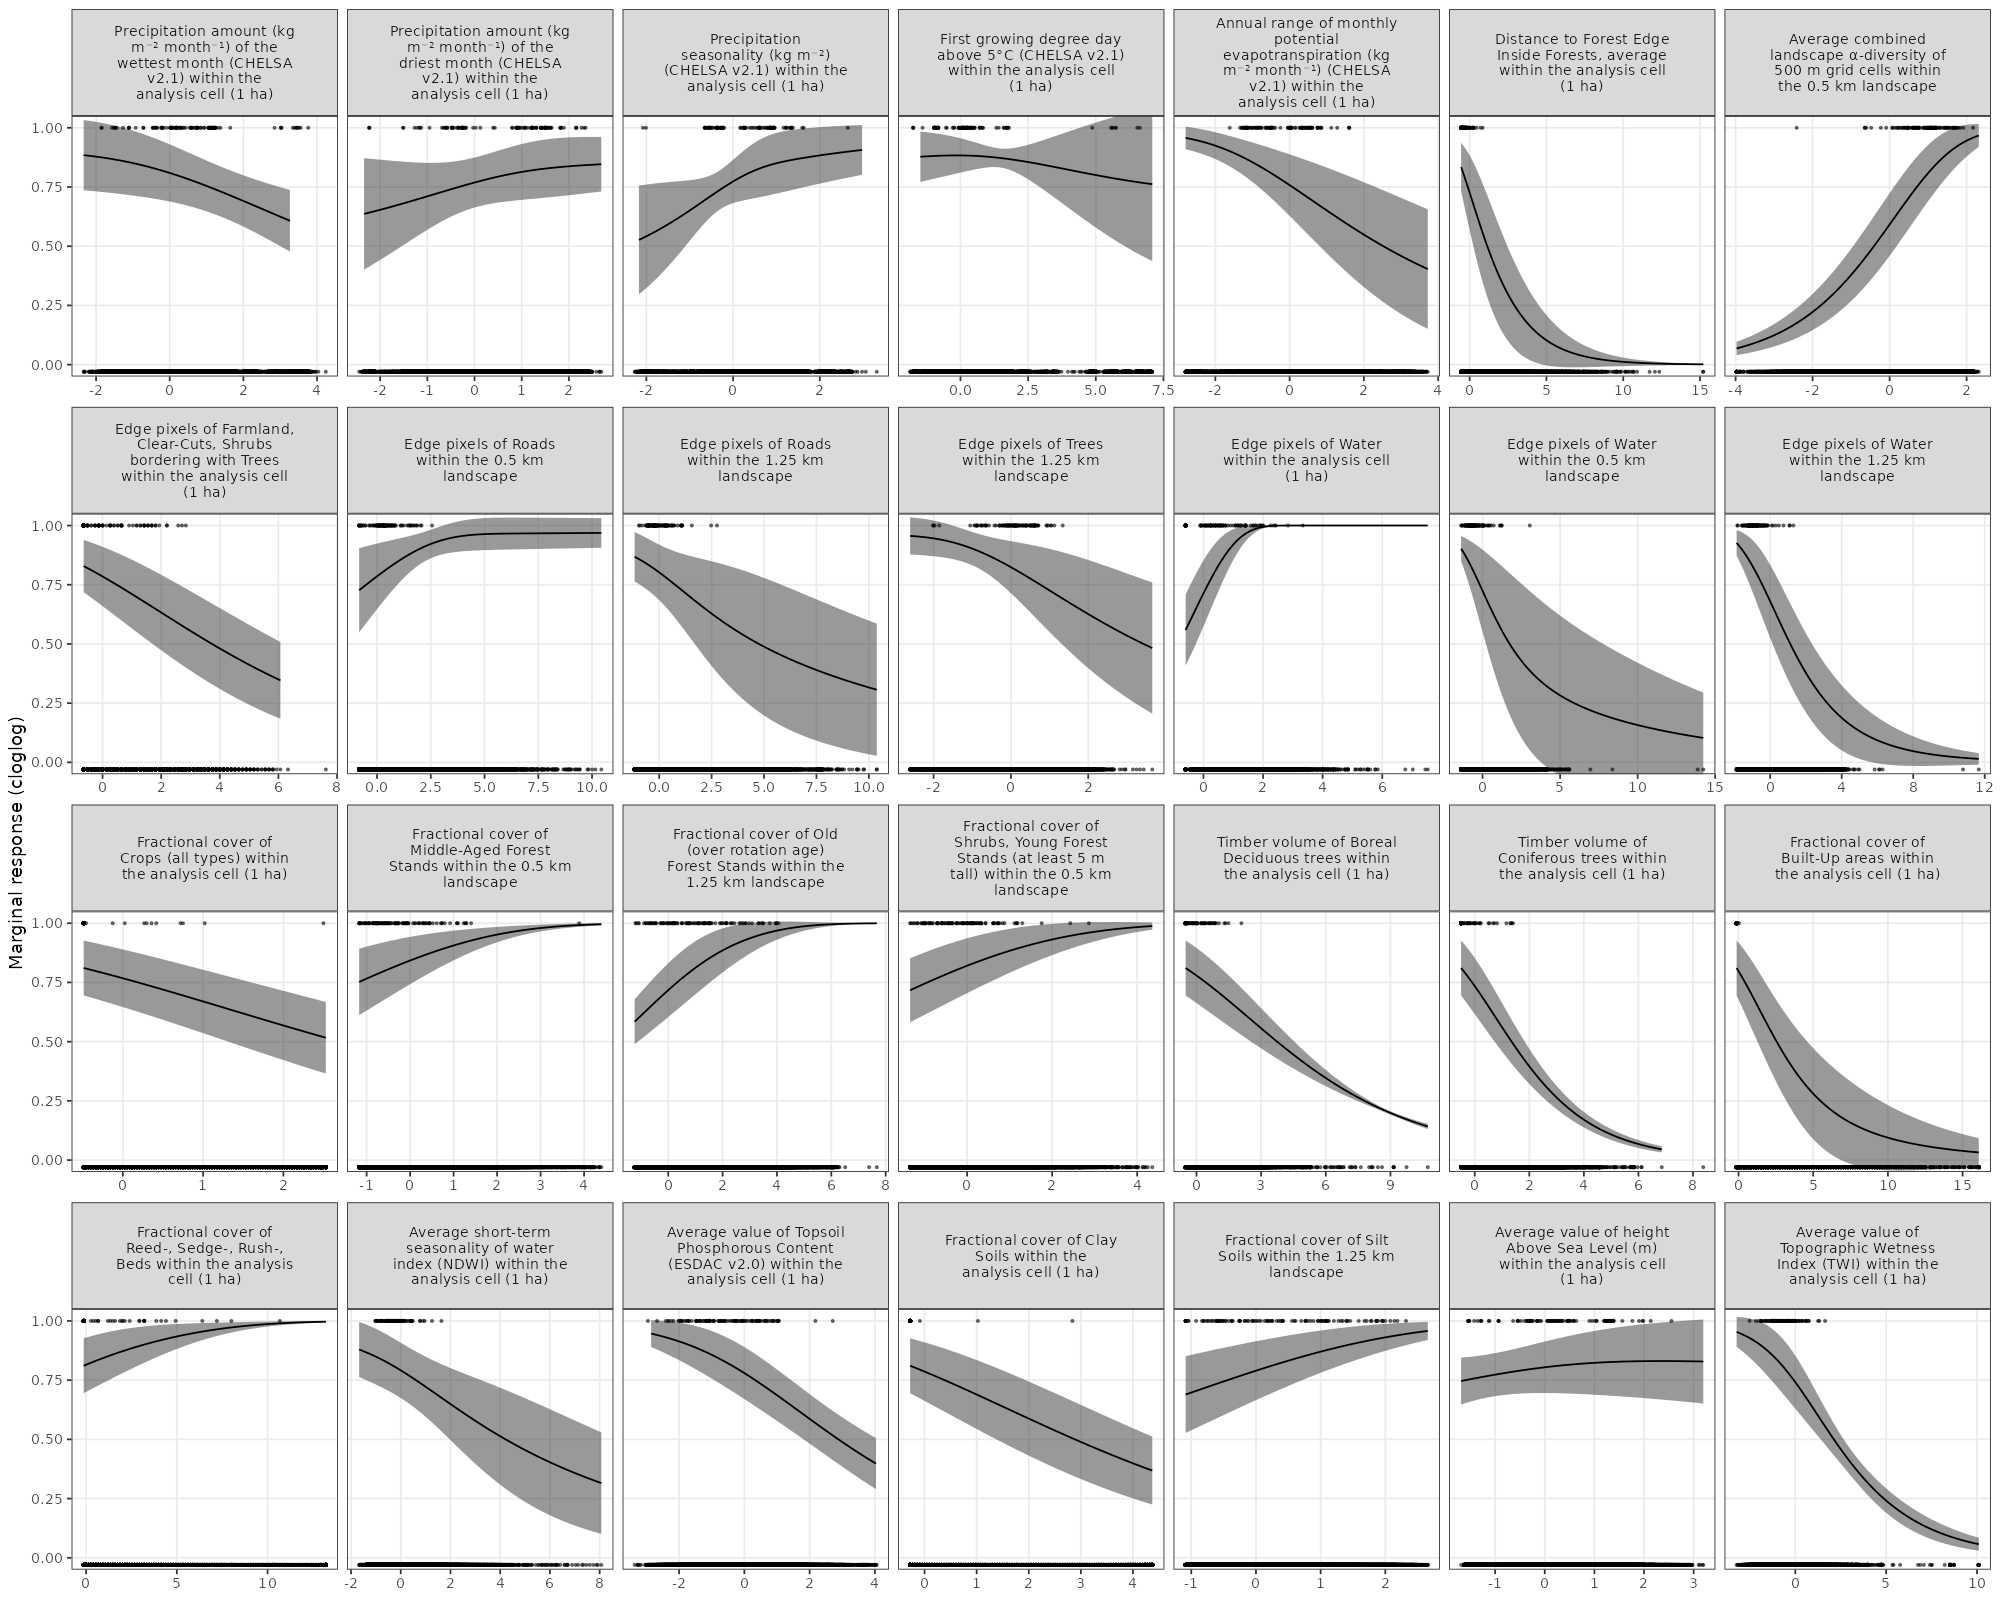
\includegraphics[width=1\linewidth,height=0.70\textheight,keepaspectratio]{results/TRICRIlarvaev2b1/PicMargResp_TRICRIlarvae.png}

\par\small\textit{Marginalised for arithmetic mean response curves illustrating the effect of each ecogeographical variable on the habitat suitability when all the other variables have their arithmetic mean values. The y-axis shows the predicted habitat suitability (cloglog-transformed), while the x-axis shows the standardised (centred and scaled) value of the ecogeographical variable. Dots at a value of 1 on the y-axis illustrate presence locations in the environment (on the x-axis), while dots at a value of 0 illustrate background locations used in modelling.  **For a full resolution refer to repository: link or online document: link**}\normalsize
\end{center}

\section*{Habitat and conservation associations}\label{habitat-and-conservation-associations-5}
\addcontentsline{toc}{section}{Habitat and conservation associations}

\begin{center}
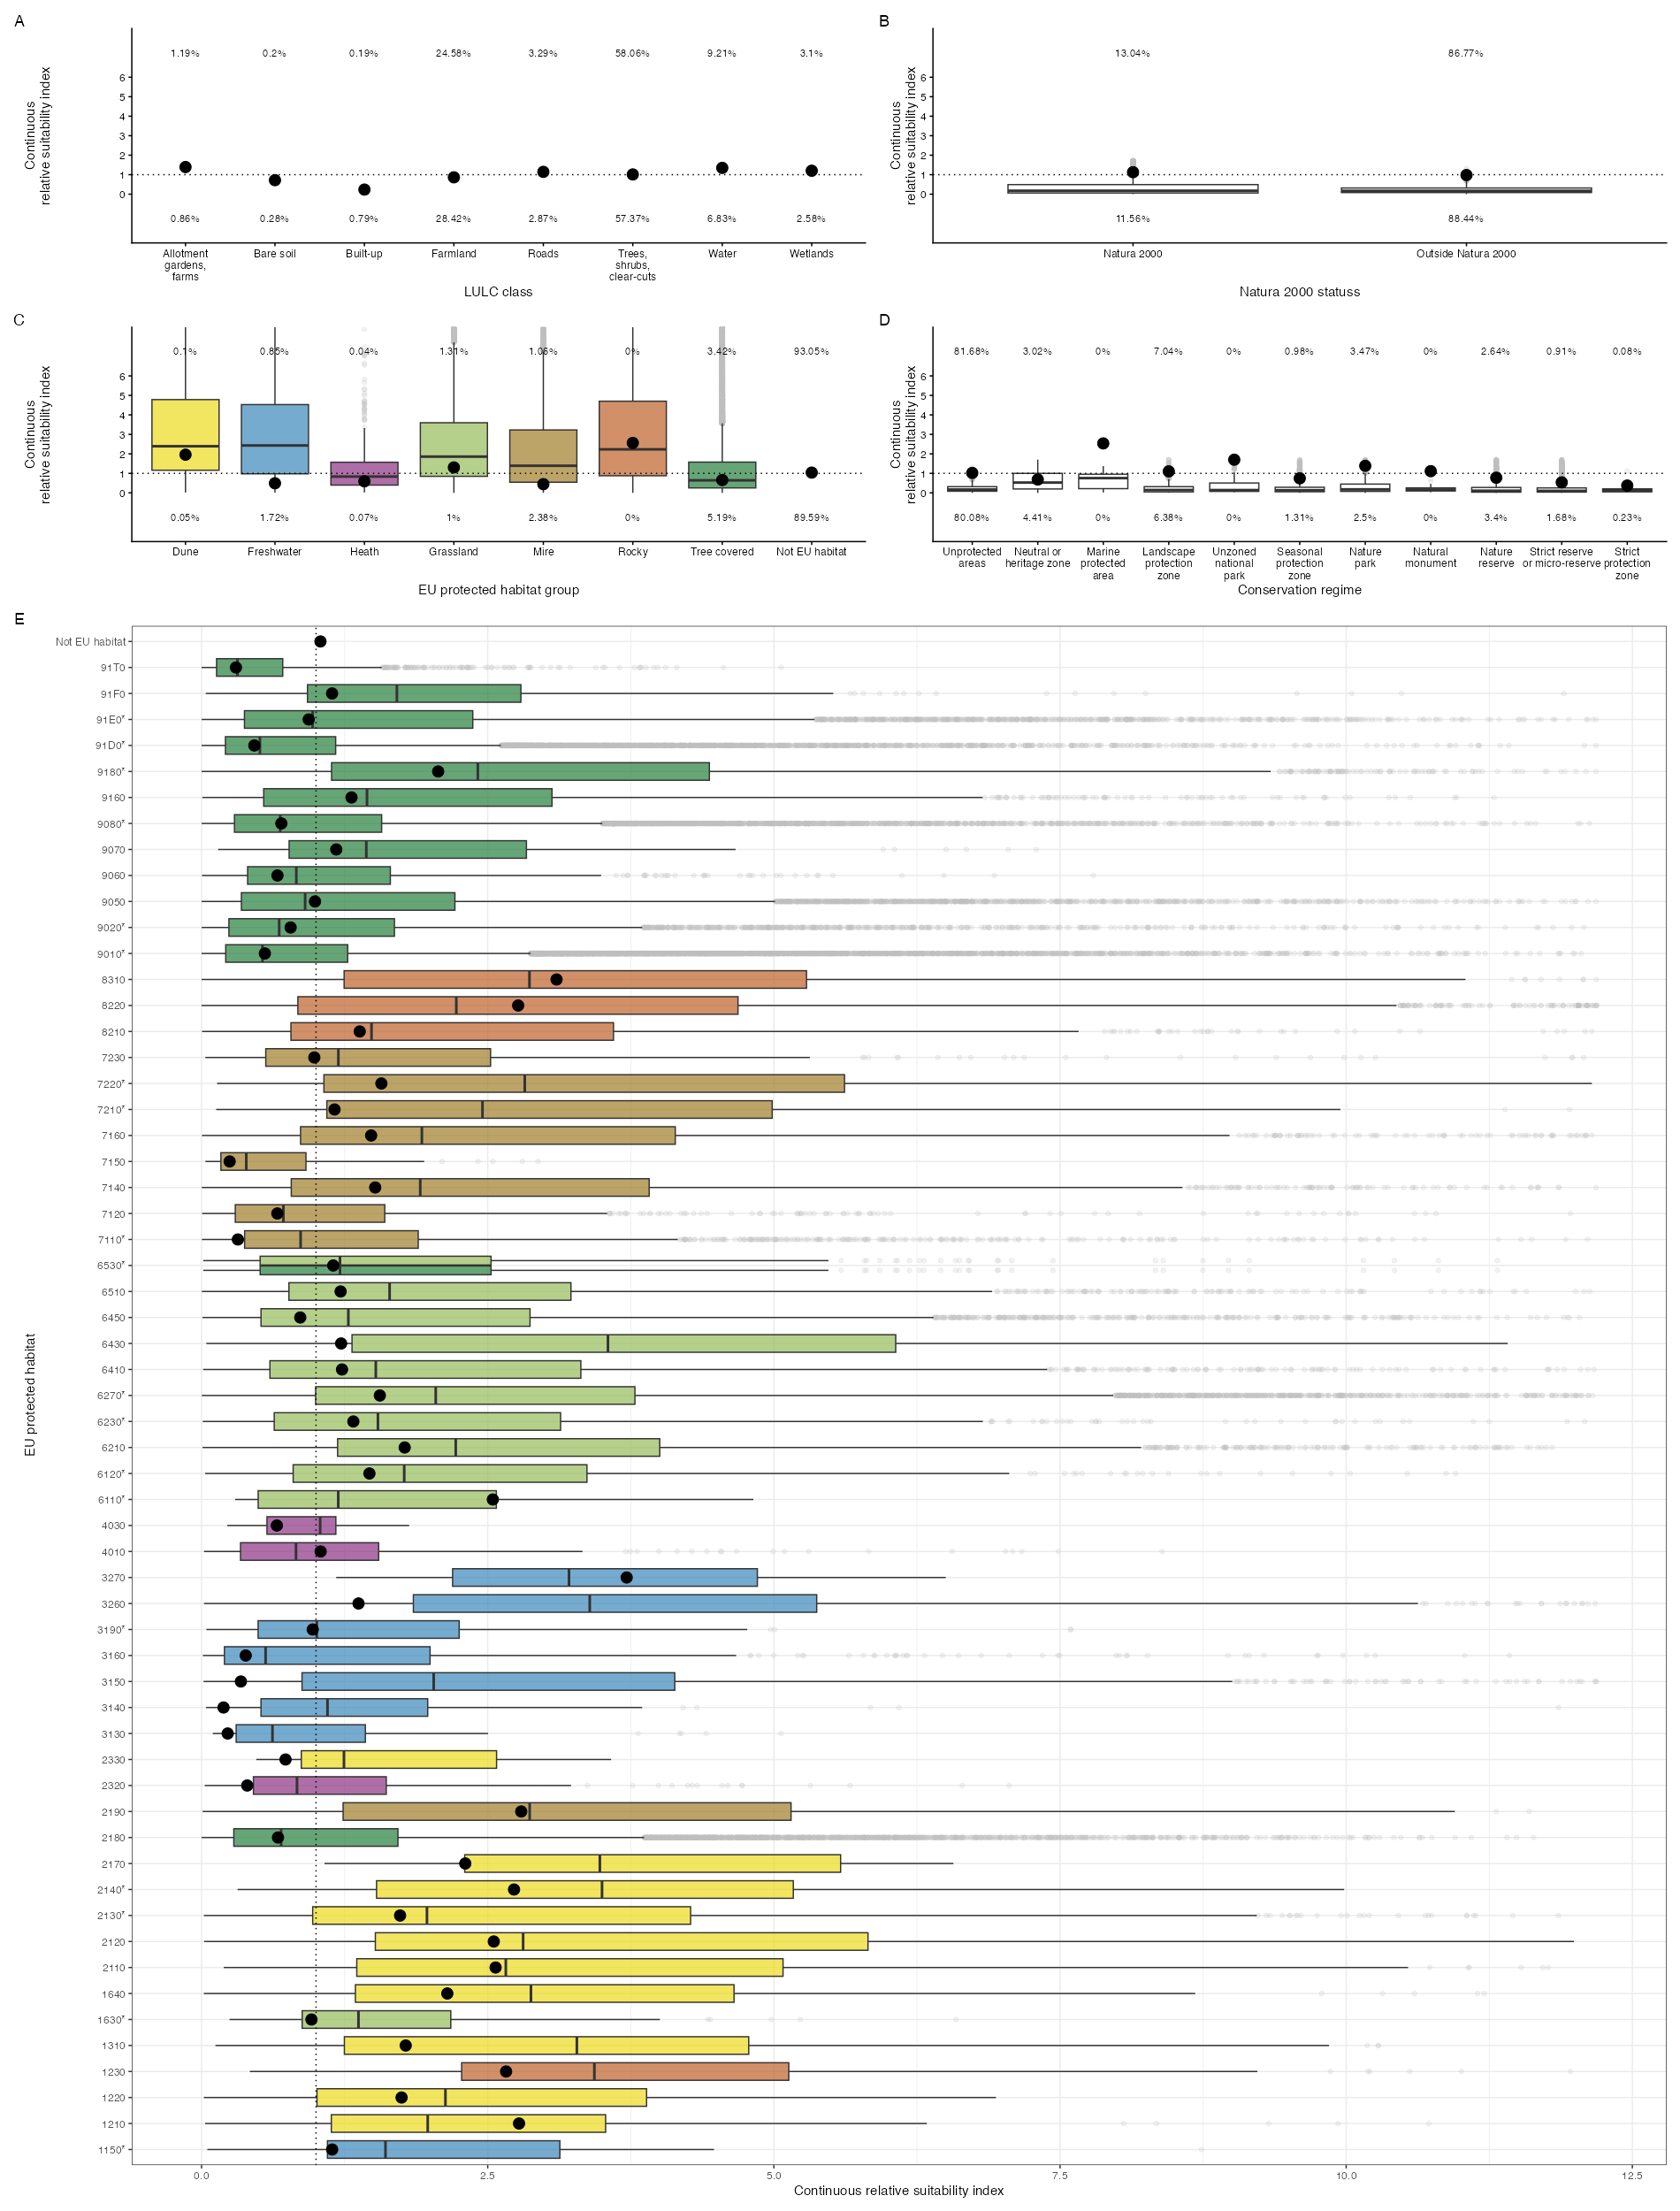
\includegraphics[width=1\linewidth,height=0.70\textheight,keepaspectratio]{results/TRICRIlarvaev2b1/PicAssoc_TRICRIlarvae.png}

\par\small\textit{Associations between predicted suitability and: (A) land use land cover classes, (B) Natura 2000 status, (C) stratified EU protected habitat classes, (D) conservation regime, and (E) EU protected habitats. The y-axis show continuous relative suitability index (derivative of Manly's index of preference). Colours in (C) and (E) correspond to stratified EU protected habitat classes. For classifications composed of multiple individual polygons, polygon-level indices were additionally calculated to show within-category variation. The figures therefore combine category-level estimates (points) with the distributions of polygon-level values (boxplots, where applicable). Labels above and below the panels report, respectively, the percentage of total predicted suitability and the percentage of mapped area represented by each category. **For a full resolution refer to repository: link or online document: link**}\normalsize
\end{center}

\section*{Conservation prioritization}\label{conservation-prioritization-5}
\addcontentsline{toc}{section}{Conservation prioritization}

\begin{center}
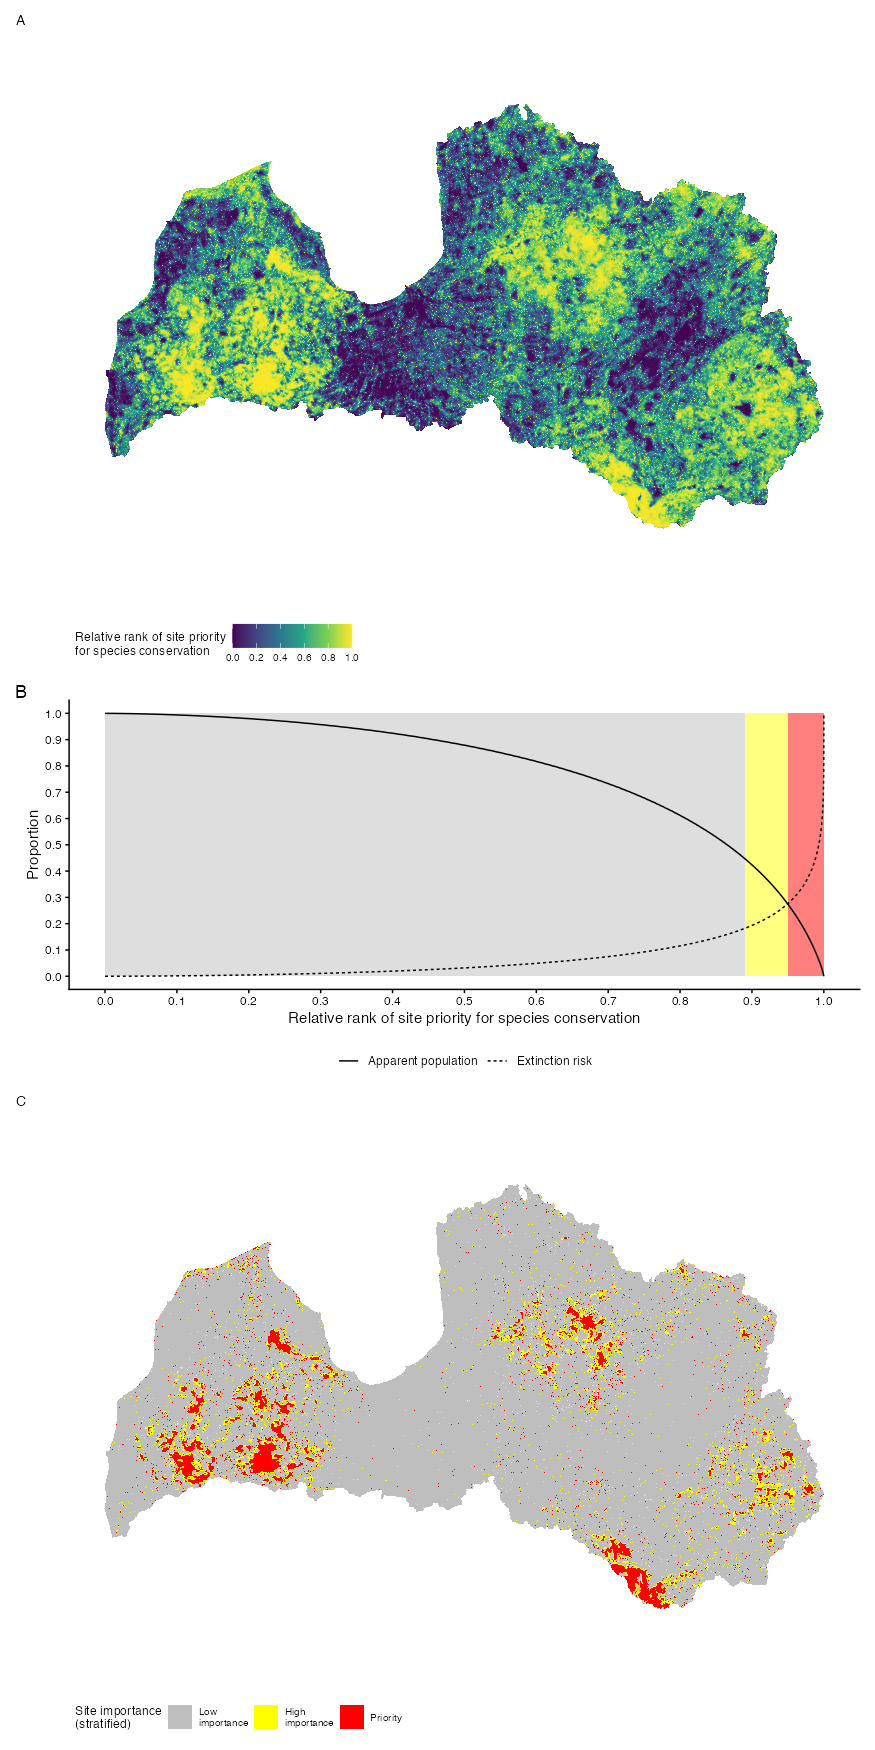
\includegraphics[width=0.85\linewidth,height=0.70\textheight,keepaspectratio]{results/TRICRIlarvaev2b1/PicPrior_TRICRIlarvae.png}

\par\small\textit{Single-species conservation prioritization focusing on maximisation of core area protection (CAZMAX) while accounting for site connectivity: (A) relative site rank; (B) relationship between apparent-population and extinction-risk curves with a simplified classification which is spatially demonstrated in the bootom row; (C) spatial distribution of proposed classification of site prioritization results. **For a full resolution refer to repository: link or online document: link**}\normalsize
\end{center}

\chapter*{\texorpdfstring{\emph{Bombina bombina}}{Bombina bombina}}\label{bombom}
\addcontentsline{toc}{chapter}{\emph{Bombina bombina}}

\section*{Summary}\label{summary-6}
\addcontentsline{toc}{section}{Summary}

\subsection*{Model description}\label{model-description-6}
\addcontentsline{toc}{subsection}{Model description}

Occurrence and background data were divided into model-training with four block spatial cross-validation data and an independent test set. Sampling-bias/background treatment: \textbf{Phenology Weighted Target Group}. Accumulated LULC change within the 1-ha analysis cell was not evaluated; accumulated LULC change within the home-range radius around the analysis cell was not evaluated.

The final data set contained \textbf{191} presence records: \textbf{143} for training with four spatial block cross-validation and \textbf{48} for independent testing. Training background contained \textbf{29949} locations, with \textbf{10051} additional independent-test background locations.

\subsection*{Expert assessment scores}\label{expert-assessment-scores-6}
\addcontentsline{toc}{subsection}{Expert assessment scores}

\begin{itemize}
\tightlist
\item
  \textbf{Marginal responses and variable importance score:} 4 (good ecological interpretability)
\item
  \textbf{Map score:} 4 (good agreement with known distribution)
\item
  \textbf{Applicability score:} 4 (high applicability)
\end{itemize}

\textbf{Šo sadaļu aizpildām manuāli no ekspertu aptaujām}

The model was considered ecologically plausible overall. Elevated suitability in
the 0.5 road-distance band was interpreted as a likely observer-access effect,
while climatic predictors showed relatively high uncertainty; otherwise, the
marginal responses were considered reasonable. The habitat-suitability map agreed
well with expert knowledge and was considered among the best of the evaluated
model variants, although some local overprediction remained, notably around
Lake Riču. The map was considered suitable for species-conservation planning
when used together with other ecological information, while the explanatory
value of the marginal response functions was somewhat more limited.

Expert: Andris Čeirāns

\subsection*{Statistical evaluation}\label{statistical-evaluation-6}
\addcontentsline{toc}{subsection}{Statistical evaluation}

The final model had a training TSS of \textbf{0.401}, with a training-derived cloglog threshold of \textbf{0.317}. Combined training AUC was \textbf{0.945} and combined test AUC was \textbf{0.877}.

\subsubsection*{Spatial cross-validation}\label{spatial-cross-validation-6}
\addcontentsline{toc}{subsubsection}{Spatial cross-validation}

\begin{itemize}
\tightlist
\item
  \textbf{AUC:} 0.7696 ± 0.0492; null models: 0.5694 ± 0.044; z = 4.5533, p \textless{} 0.001
\item
  \textbf{CBI:} 0.812 ± 0.1155; null models: 0.2354 ± 0.1514; z = 3.8093, p \textless{} 0.001
\item
  \textbf{OR10:} 0.2875 ± 0.111; null models: 0.144 ± 0.0972; z = 1.4763, p = 0.93
\item
  \textbf{ORmin:} 0.0139 ± 0.016; null models: 0.0621 ± 0.0823; z = -0.5853, p = 0.279
\end{itemize}

\subsubsection*{Independent testing}\label{independent-testing-6}
\addcontentsline{toc}{subsubsection}{Independent testing}

\begin{itemize}
\tightlist
\item
  \textbf{TSS:} 0.509; \textbf{sensitivity:} 0.729; \textbf{specificity:} 0.78
\item
  \textbf{AUC:} 0.903; null models: 0.518 ± 0.1496; z = 2.5716, p = 0.005
\item
  \textbf{CBI:} 0.879; null models: -0.0028 ± 0.4837; z = 1.8232, p = 0.034
\item
  \textbf{OR10:} 0.312; null models: 0.129 ± 0.1642; z = 1.118, p = 0.868
\item
  \textbf{ORmin:} 0.042; null models: 0.0065 ± 0.0264; z = 1.3319, p = 0.909
\end{itemize}

\subsection*{Conservation prioritisation summary}\label{conservation-prioritisation-summary-6}
\addcontentsline{toc}{subsection}{Conservation prioritisation summary}

The primary priority area covers \textbf{2\%} of Latvia and contains \textbf{27.6\%} of the summed habitat suitability (apparent population proxy).

The broader high importance area covers \textbf{3.1\%} of Latvia and contains \textbf{35.7\%} of the summed habitat suitability.

For comparison, the area classified as suitable using the maximum training sensitivity plus specificity habitat-suitability threshold contains \textbf{35.7\%} of the summed continuous habitat suitability.

\subsection*{Version evolution}\label{version-evolution-6}
\addcontentsline{toc}{subsection}{Version evolution}

\textbf{Šo sadaļu aizpildām manuāli, izmntojot sagatavotās shēmas. Jāvienojas par to noformējumu}

The following diagram describes version evolution during modelling.
Colour codes:

\begin{itemize}
\item
  \textbf{black}: branch in version evolution from the initial EGV selection up
  until the best version;
\item
  \textbf{green}: the final version;
\item
  \textbf{grey}: other versions.
\end{itemize}

All the modifications on the black-to-green branch are described below the
diagram.

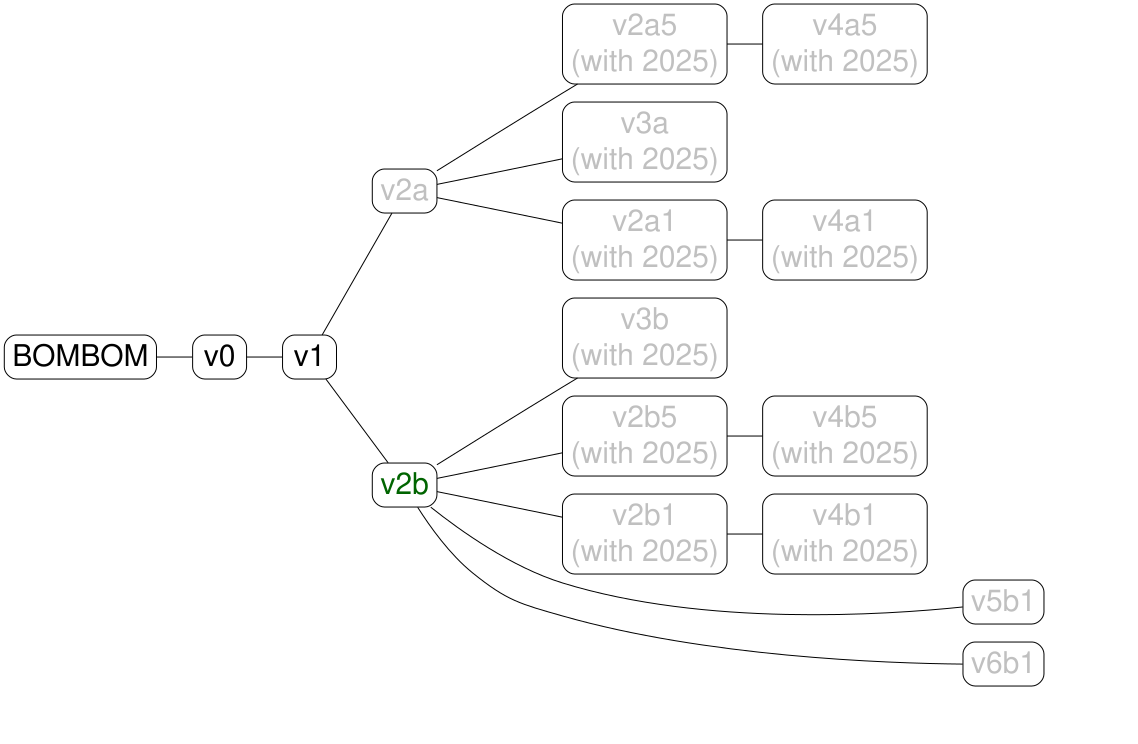
\includegraphics[width=1\linewidth]{figures/version_evolution/BOMBOM_version_evolution}

\textbf{v0 to v1}

\begin{itemize}
\item
  EGVs excluded:

  \begin{itemize}
  \item
    egv\_150: (Edges\_Roads\_cell.tif) Edge pixels of Roads within the analysis cell (1 ha)
  \item
    egv\_423: (General\_ForestsWithoutInventory\_cell.tif) Fractional cover of Forests Without Inventory within the analysis cell (1 ha)
  \item
    egv\_424: (General\_ForestsWithoutInventory\_r500.tif) Fractional cover of Forests Without Inventory within the 0.5 km landscape
  \item
    egv\_425: (General\_ForestsWithoutInventory\_r1250.tif) Fractional cover of Forests Without Inventory within the 1.25 km landscape
  \item
    egv\_426: (General\_ForestsWithoutInventory\_r3000.tif) Fractional cover of Forests Without Inventory within the 3 km landscape
  \item
    egv\_427: (General\_ForestsWithoutInventory\_r10000.tif) Fractional cover of Forests Without Inventory within the 10 km landscape
  \item
    egv\_255: (FarmlandSubsidies\_BiologicalSubsidies\_cell.tif) Fractional cover of Farmland receiving Subsidies for Biological Agriculture within the analysis cell (1 ha)
  \item
    egv\_256: (FarmlandSubsidies\_BiologicalSubsidies\_r500.tif) Fractional cover of Farmland receiving Subsidies for Biological Agriculture within the 0.5 km landscape
  \item
    egv\_257: (FarmlandSubsidies\_BiologicalSubsidies\_r1250.tif) Fractional cover of Farmland receiving Subsidies for Biological Agriculture within the 1.25 km landscape
  \item
    egv\_258: (FarmlandSubsidies\_BiologicalSubsidies\_r3000.tif) Fractional cover of Farmland receiving Subsidies for Biological Agriculture within the 3 km landscape
  \item
    egv\_259: (FarmlandSubsidies\_BiologicalSubsidies\_r10000.tif) Fractional cover of Farmland receiving Subsidies for Biological Agriculture within the 10 km landscape
  \end{itemize}
\end{itemize}

\textbf{v1 to v2b}

\begin{itemize}
\item
  EGVs excluded:

  \begin{itemize}
  \tightlist
  \item
    egv\_093: (Distance\_Sea\_cell.tif) Distance to Sea, average within the analysis cell (1 ha)
  \end{itemize}
\item
  LULC change since the year of observation until the year 2024 are not used in
  observation filtering.
\end{itemize}

\section*{Habitat suitability}\label{habitat-suitability-6}
\addcontentsline{toc}{section}{Habitat suitability}

\begin{center}
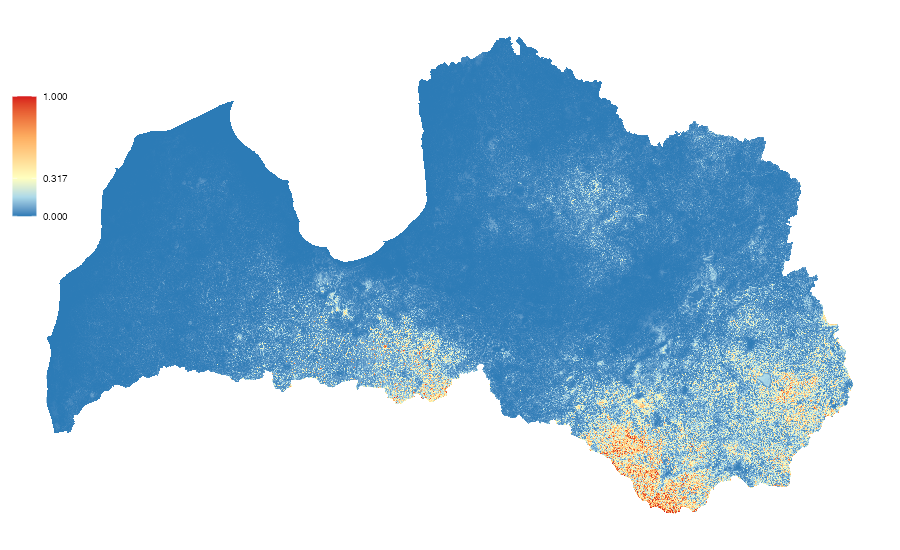
\includegraphics[width=1\linewidth,height=0.70\textheight,keepaspectratio]{results/BOMBOMv2b/PicHSmap_BOMBOM.png}

\par\small\textit{Predicted continuous habitat suitability across Latvia. The warmer the colour the higher is the predicted habitat suitability. Value in the middle of the legend correspond to the maximum training sensitivity plus specificity threshold. **For a full resolution refer to repository: link or online document: link**}\normalsize
\end{center}

\section*{Model thresholds}\label{model-thresholds-6}
\addcontentsline{toc}{section}{Model thresholds}

Threshold values and associated omission rates

\begin{center}
\resizebox{\linewidth}{!}{%

\begin{tabular}{lrrrrr}
\toprule
Threshold & Cloglog value & Fractional predicted area & Training omission rate & Test omission rate & P-values\\
\midrule
Minimum training presence & 0.1182659 & 0.2667422 & 0.0000000 & 0.0001978 & 0\\
Equal training sensitivity and specificity & 0.4227094 & 0.1241041 & 0.1258741 & 0.0014837 & 0\\
Maximum training sensitivity plus specificity & 0.3166795 & 0.1614720 & 0.0349650 & 0.0012859 & 0\\
Equal test sensitivity and specificity & 0.2771921 & 0.1762725 & 0.0279720 & 0.0010880 & 0\\
Maximum test sensitivity plus specificity & 0.1062868 & 0.2765426 & 0.0000000 & 0.0000000 & 0\\
\bottomrule
\end{tabular}
}
\end{center}

\section*{Variable importance}\label{variable-importance-6}
\addcontentsline{toc}{section}{Variable importance}

\begin{center}
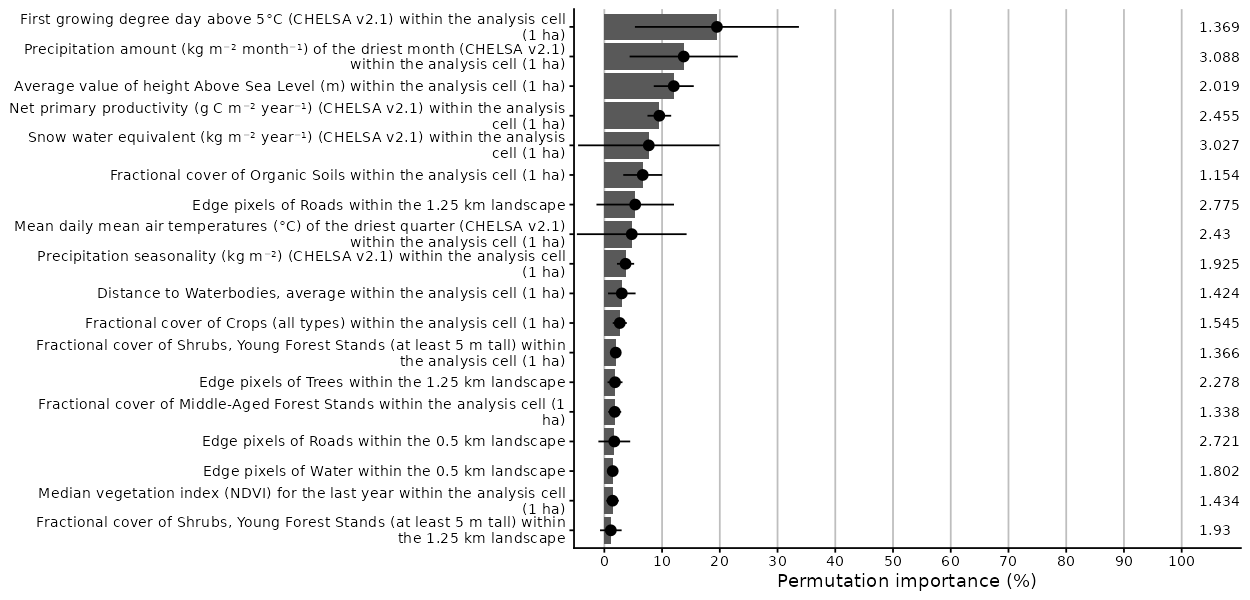
\includegraphics[width=1\linewidth,height=0.70\textheight,keepaspectratio]{results/BOMBOMv2b/PicVarImpVIFs_BOMBOM.png}

\par\small\textit{Permutation-importance (mean and standard deviation from 99 permutations, on the x-axis) of the ecogeographical variables (first y-axis, left side), and their variance inflation factor values (second y-axis, right side). **For a full resolution refer to repository: link or online document: link**}\normalsize
\end{center}

\section*{Marginal responses}\label{marginal-responses-6}
\addcontentsline{toc}{section}{Marginal responses}

\begin{center}
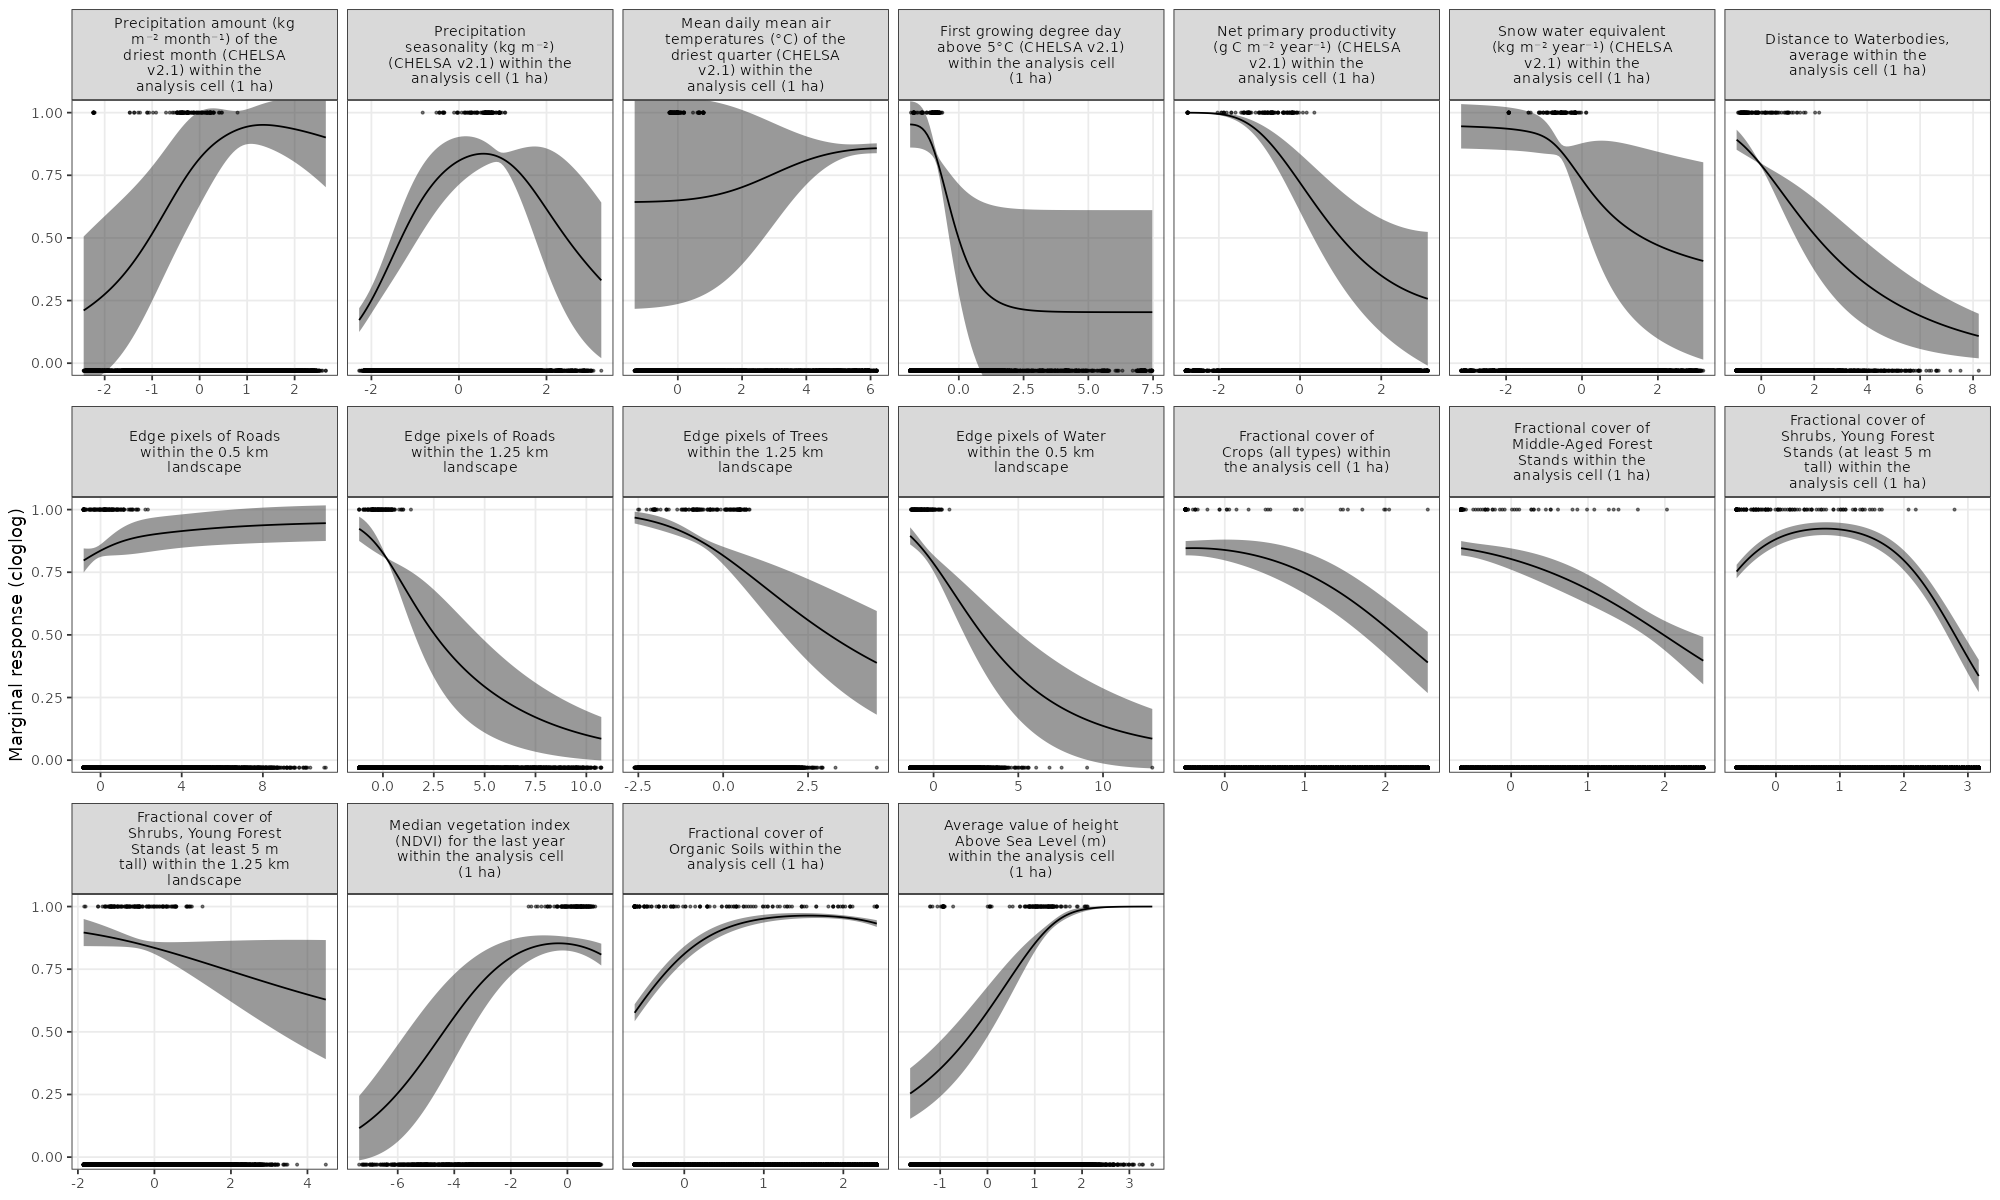
\includegraphics[width=1\linewidth,height=0.70\textheight,keepaspectratio]{results/BOMBOMv2b/PicMargResp_BOMBOM.png}

\par\small\textit{Marginalised for arithmetic mean response curves illustrating the effect of each ecogeographical variable on the habitat suitability when all the other variables have their arithmetic mean values. The y-axis shows the predicted habitat suitability (cloglog-transformed), while the x-axis shows the standardised (centred and scaled) value of the ecogeographical variable. Dots at a value of 1 on the y-axis illustrate presence locations in the environment (on the x-axis), while dots at a value of 0 illustrate background locations used in modelling.  **For a full resolution refer to repository: link or online document: link**}\normalsize
\end{center}

\section*{Habitat and conservation associations}\label{habitat-and-conservation-associations-6}
\addcontentsline{toc}{section}{Habitat and conservation associations}

\begin{center}
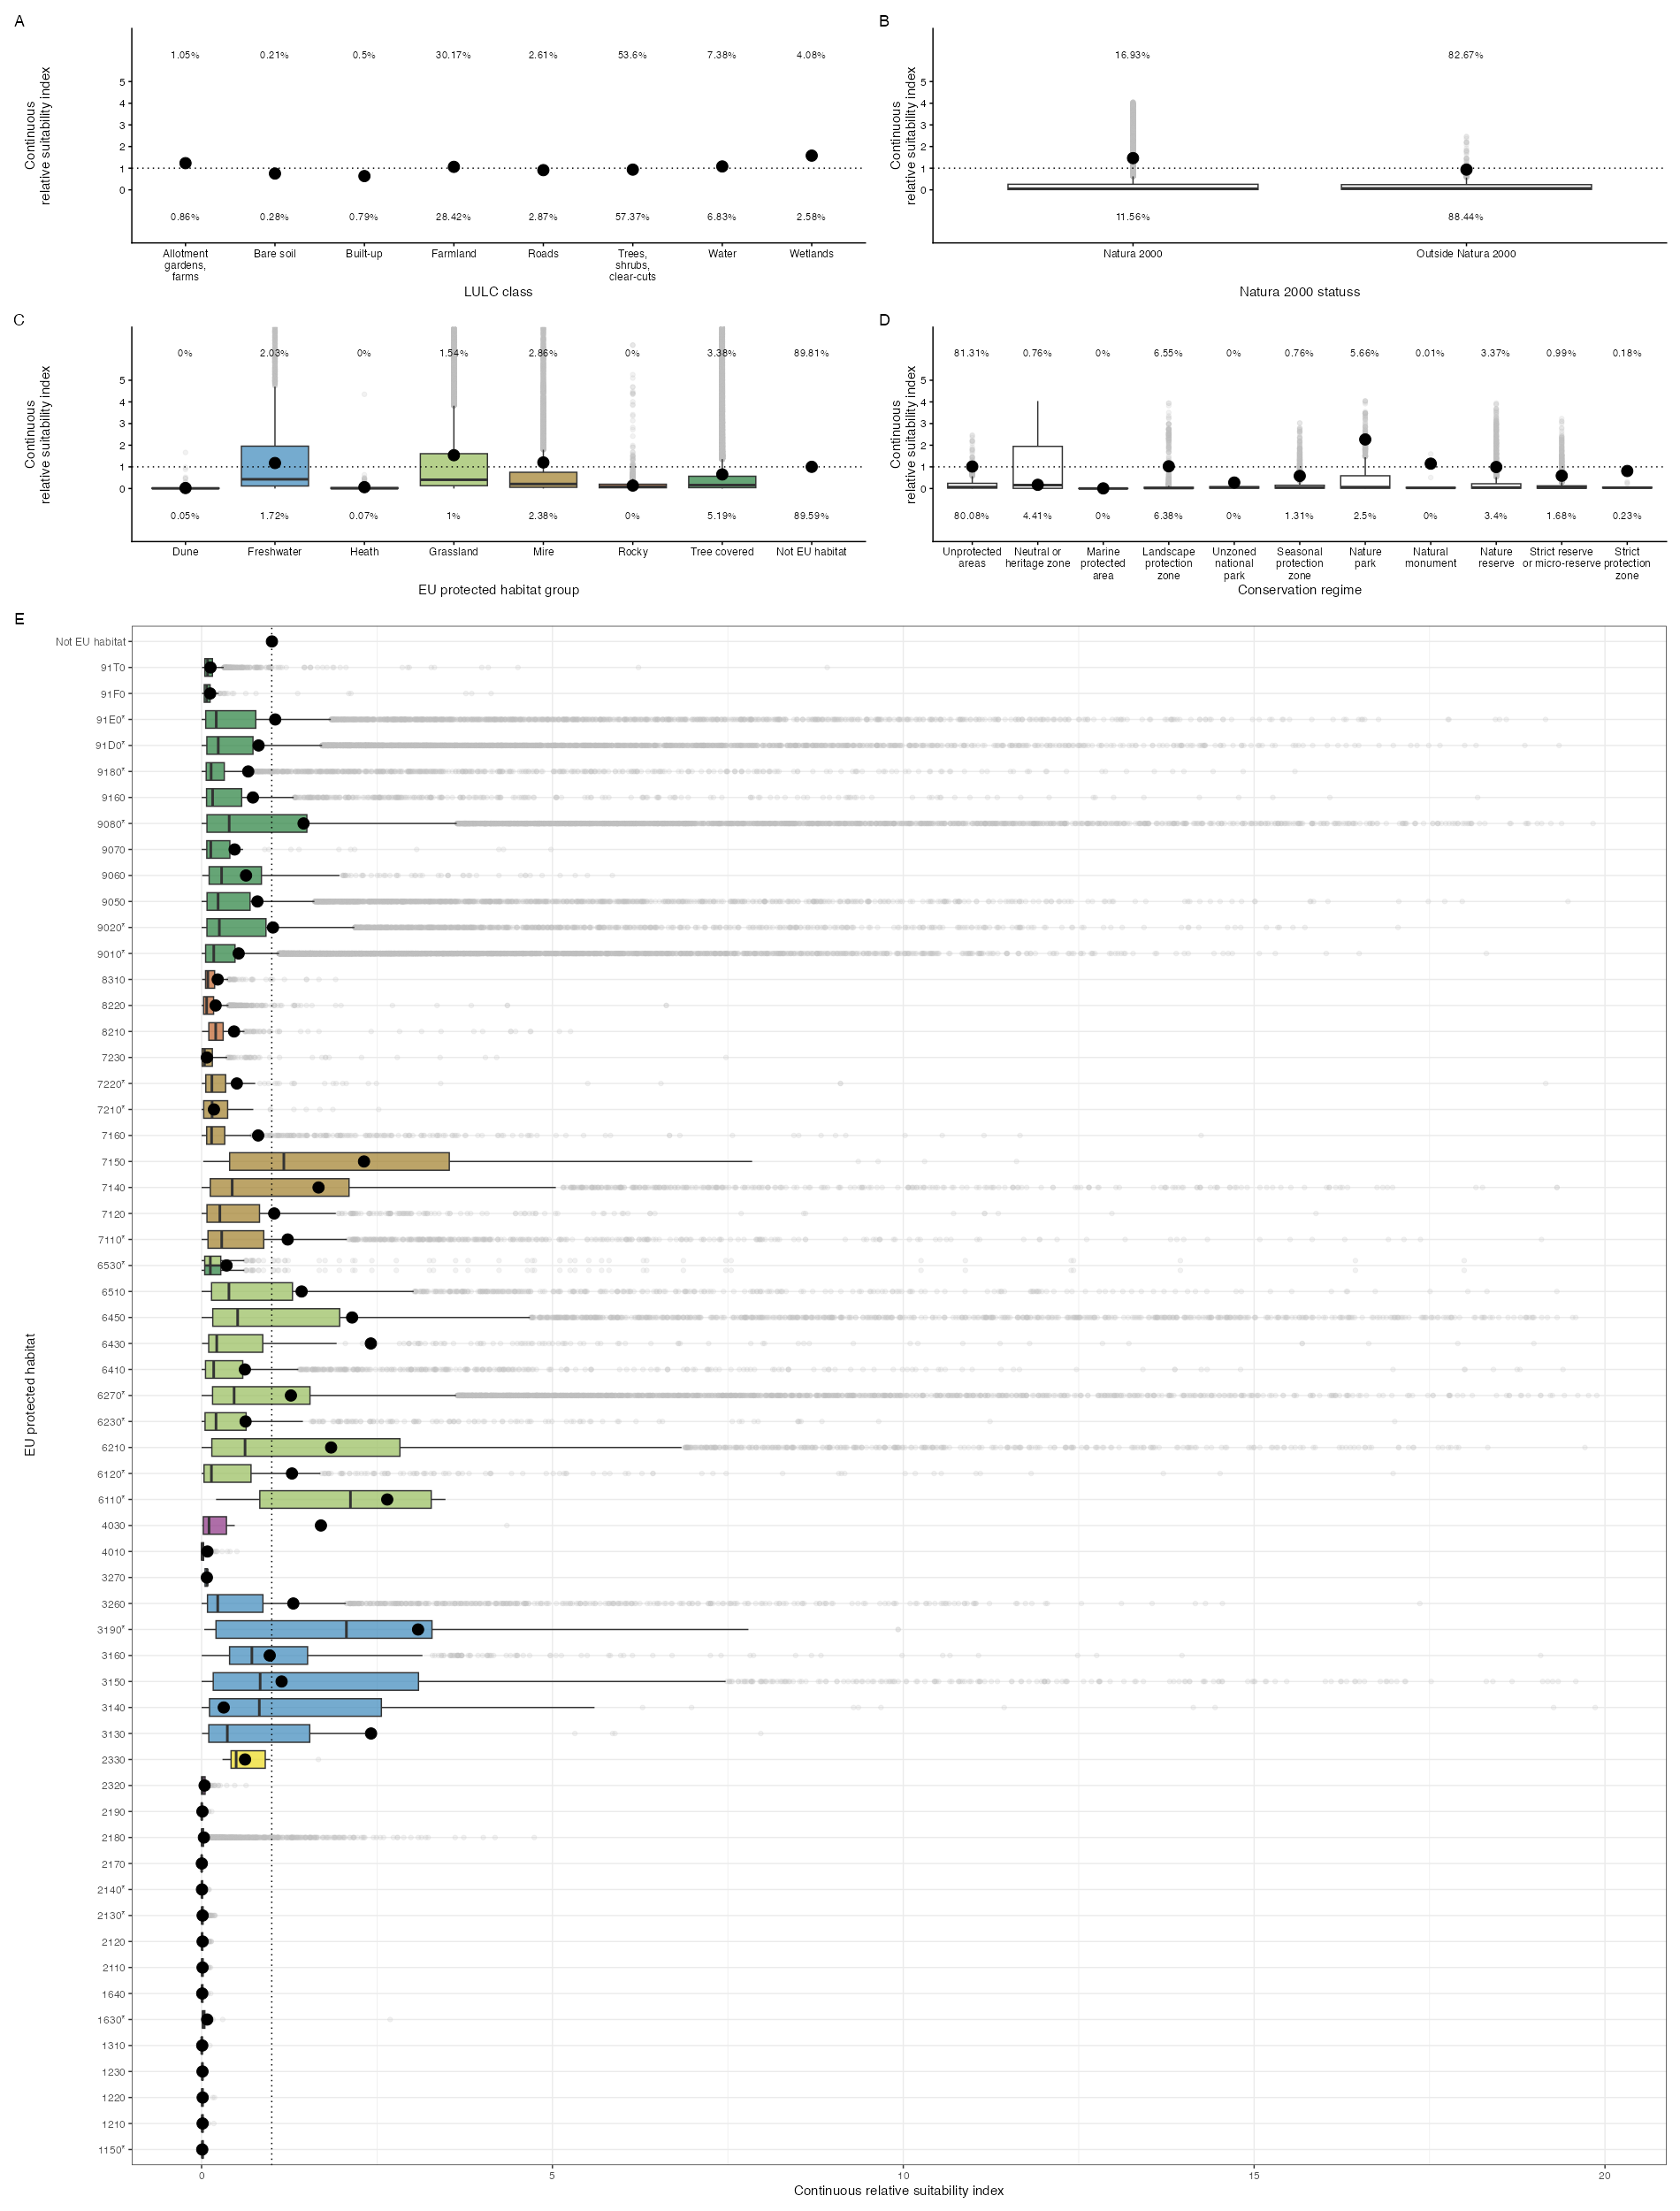
\includegraphics[width=1\linewidth,height=0.70\textheight,keepaspectratio]{results/BOMBOMv2b/PicAssoc_BOMBOM.png}

\par\small\textit{Associations between predicted suitability and: (A) land use land cover classes, (B) Natura 2000 status, (C) stratified EU protected habitat classes, (D) conservation regime, and (E) EU protected habitats. The y-axis show continuous relative suitability index (derivative of Manly's index of preference). Colours in (C) and (E) correspond to stratified EU protected habitat classes. For classifications composed of multiple individual polygons, polygon-level indices were additionally calculated to show within-category variation. The figures therefore combine category-level estimates (points) with the distributions of polygon-level values (boxplots, where applicable). Labels above and below the panels report, respectively, the percentage of total predicted suitability and the percentage of mapped area represented by each category. **For a full resolution refer to repository: link or online document: link**}\normalsize
\end{center}

\section*{Conservation prioritization}\label{conservation-prioritization-6}
\addcontentsline{toc}{section}{Conservation prioritization}

\begin{center}
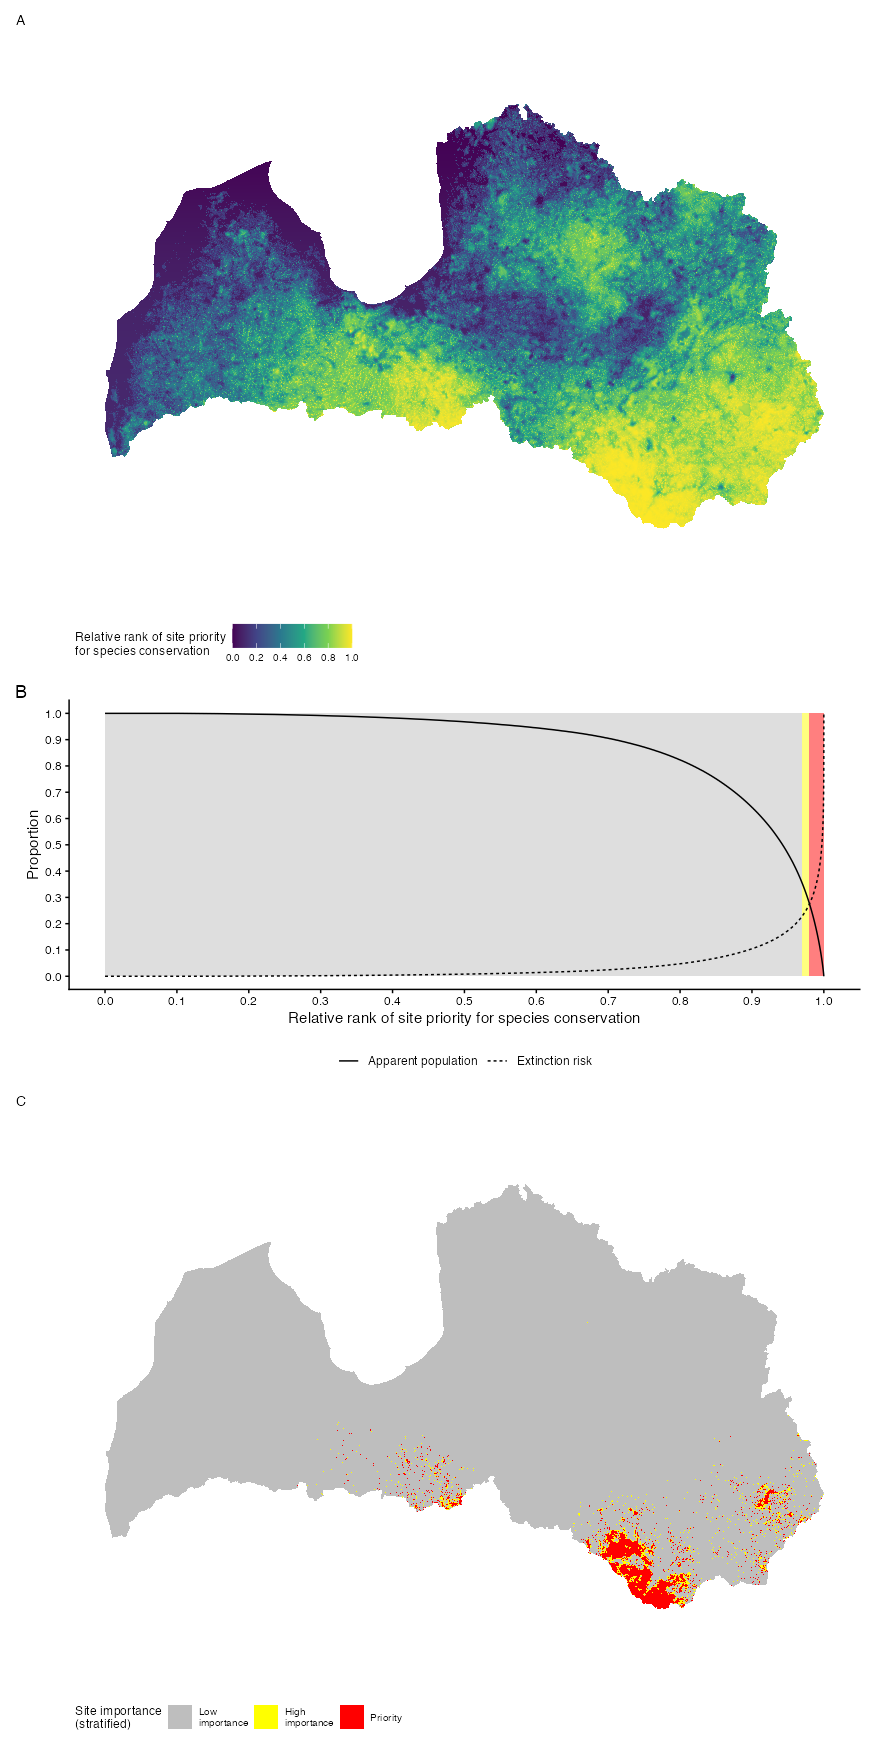
\includegraphics[width=0.85\linewidth,height=0.70\textheight,keepaspectratio]{results/BOMBOMv2b/PicPrior_BOMBOM.png}

\par\small\textit{Single-species conservation prioritization focusing on maximisation of core area protection (CAZMAX) while accounting for site connectivity: (A) relative site rank; (B) relationship between apparent-population and extinction-risk curves with a simplified classification which is spatially demonstrated in the bootom row; (C) spatial distribution of proposed classification of site prioritization results. **For a full resolution refer to repository: link or online document: link**}\normalsize
\end{center}

\chapter*{\texorpdfstring{\emph{Pelobates fuscus}}{Pelobates fuscus}}\label{pelfus}
\addcontentsline{toc}{chapter}{\emph{Pelobates fuscus}}

\section*{Summary}\label{summary-7}
\addcontentsline{toc}{section}{Summary}

\subsection*{Model description}\label{model-description-7}
\addcontentsline{toc}{subsection}{Model description}

Occurrence and background data were divided into model-training with four block spatial cross-validation data and an independent test set. Sampling-bias/background treatment: \textbf{Phenology Weighted Target Group}. Accumulated LULC change within the 1-ha analysis cell was not evaluated; accumulated LULC change within the home-range radius around the analysis cell was not evaluated.

The final data set contained \textbf{182} presence records: \textbf{136} for training with four spatial block cross-validation and \textbf{46} for independent testing. Training background contained \textbf{29898} locations, with \textbf{10102} additional independent-test background locations.

\subsection*{Expert assessment scores}\label{expert-assessment-scores-7}
\addcontentsline{toc}{subsection}{Expert assessment scores}

\begin{itemize}
\tightlist
\item
  \textbf{Marginal responses and variable importance score:} 3 (moderate ecological interpretability)
\item
  \textbf{Map score:} 3 (moderate agreement with known distribution)
\item
  \textbf{Applicability score:} 3 (moderate applicability)
\end{itemize}

\textbf{Šo sadaļu aizpildām manuāli no ekspertu aptaujām}

\subsection*{Statistical evaluation}\label{statistical-evaluation-7}
\addcontentsline{toc}{subsection}{Statistical evaluation}

The final model had a training TSS of \textbf{0.401}, with a training-derived cloglog threshold of \textbf{0.483}. Combined training AUC was \textbf{0.874} and combined test AUC was \textbf{0.722}.

\subsubsection*{Spatial cross-validation}\label{spatial-cross-validation-7}
\addcontentsline{toc}{subsubsection}{Spatial cross-validation}

\begin{itemize}
\tightlist
\item
  \textbf{AUC:} 0.7936 ± 0.0139; null models: 0.5515 ± 0.0369; z = 6.5663, p \textless{} 0.001
\item
  \textbf{CBI:} 0.8268 ± 0.0591; null models: 0.2156 ± 0.166; z = 3.6815, p \textless{} 0.001
\item
  \textbf{OR10:} 0.2426 ± 0.111; null models: 0.1917 ± 0.124; z = 0.4108, p = 0.659
\item
  \textbf{ORmin:} 0.0809 ± 0.0282; null models: 0.0371 ± 0.0886; z = 0.4938, p = 0.689
\end{itemize}

\subsubsection*{Independent testing}\label{independent-testing-7}
\addcontentsline{toc}{subsubsection}{Independent testing}

\begin{itemize}
\tightlist
\item
  \textbf{TSS:} 0.285; \textbf{sensitivity:} 0.478; \textbf{specificity:} 0.806
\item
  \textbf{AUC:} 0.713; null models: 0.5061 ± 0.0657; z = 3.1404, p = 0.001
\item
  \textbf{CBI:} 0.73; null models: 0.0594 ± 0.4009; z = 1.6728, p = 0.047
\item
  \textbf{OR10:} 0.326; null models: 0.1891 ± 0.0883; z = 1.5512, p = 0.94
\item
  \textbf{ORmin:} 0.196; null models: 0.0122 ± 0.0226; z = 8.132, p = 1
\end{itemize}

\subsection*{Conservation prioritisation summary}\label{conservation-prioritisation-summary-7}
\addcontentsline{toc}{subsection}{Conservation prioritisation summary}

The primary priority area covers \textbf{7.2\%} of Latvia and contains \textbf{27.6\%} of the summed habitat suitability (apparent population proxy).

The broader high importance area covers \textbf{13.1\%} of Latvia and contains \textbf{42.3\%} of the summed habitat suitability.

For comparison, the area classified as suitable using the maximum training sensitivity plus specificity habitat-suitability threshold contains \textbf{42.3\%} of the summed continuous habitat suitability.

\subsection*{Version evolution}\label{version-evolution-7}
\addcontentsline{toc}{subsection}{Version evolution}

\textbf{Šo sadaļu aizpildām manuāli, izmntojot sagatavotās shēmas. Jāvienojas par to noformējumu}

\section*{Habitat suitability}\label{habitat-suitability-7}
\addcontentsline{toc}{section}{Habitat suitability}

\begin{center}
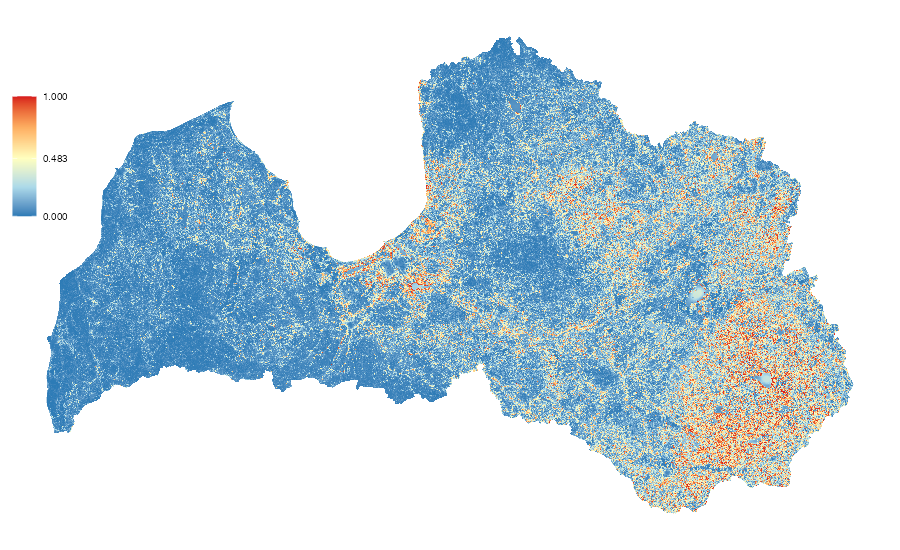
\includegraphics[width=1\linewidth,height=0.70\textheight,keepaspectratio]{results/PELFUSv2b/PicHSmap_PELFUS.png}

\par\small\textit{Predicted continuous habitat suitability across Latvia. The warmer the colour the higher is the predicted habitat suitability. Value in the middle of the legend correspond to the maximum training sensitivity plus specificity threshold. **For a full resolution refer to repository: link or online document: link**}\normalsize
\end{center}

\section*{Model thresholds}\label{model-thresholds-7}
\addcontentsline{toc}{section}{Model thresholds}

Threshold values and associated omission rates

\begin{center}
\resizebox{\linewidth}{!}{%

\begin{tabular}{lrrrrr}
\toprule
Threshold & Cloglog value & Fractional predicted area & Training omission rate & Test omission rate & P-values\\
\midrule
Minimum training presence & 0.1288130 & 0.5822506 & 0.0000000 & 0.0008852 & 0\\
Equal training sensitivity and specificity & 0.4891850 & 0.2105615 & 0.2132353 & 0.0024589 & 0\\
Maximum training sensitivity plus specificity & 0.4825414 & 0.2143024 & 0.1838235 & 0.0023606 & 0\\
Equal test sensitivity and specificity & 0.3130393 & 0.3391563 & 0.0955882 & 0.0014754 & 0\\
Maximum test sensitivity plus specificity & 0.3442167 & 0.3123685 & 0.1250000 & 0.0014754 & 0\\
\bottomrule
\end{tabular}
}
\end{center}

\section*{Variable importance}\label{variable-importance-7}
\addcontentsline{toc}{section}{Variable importance}

\begin{center}
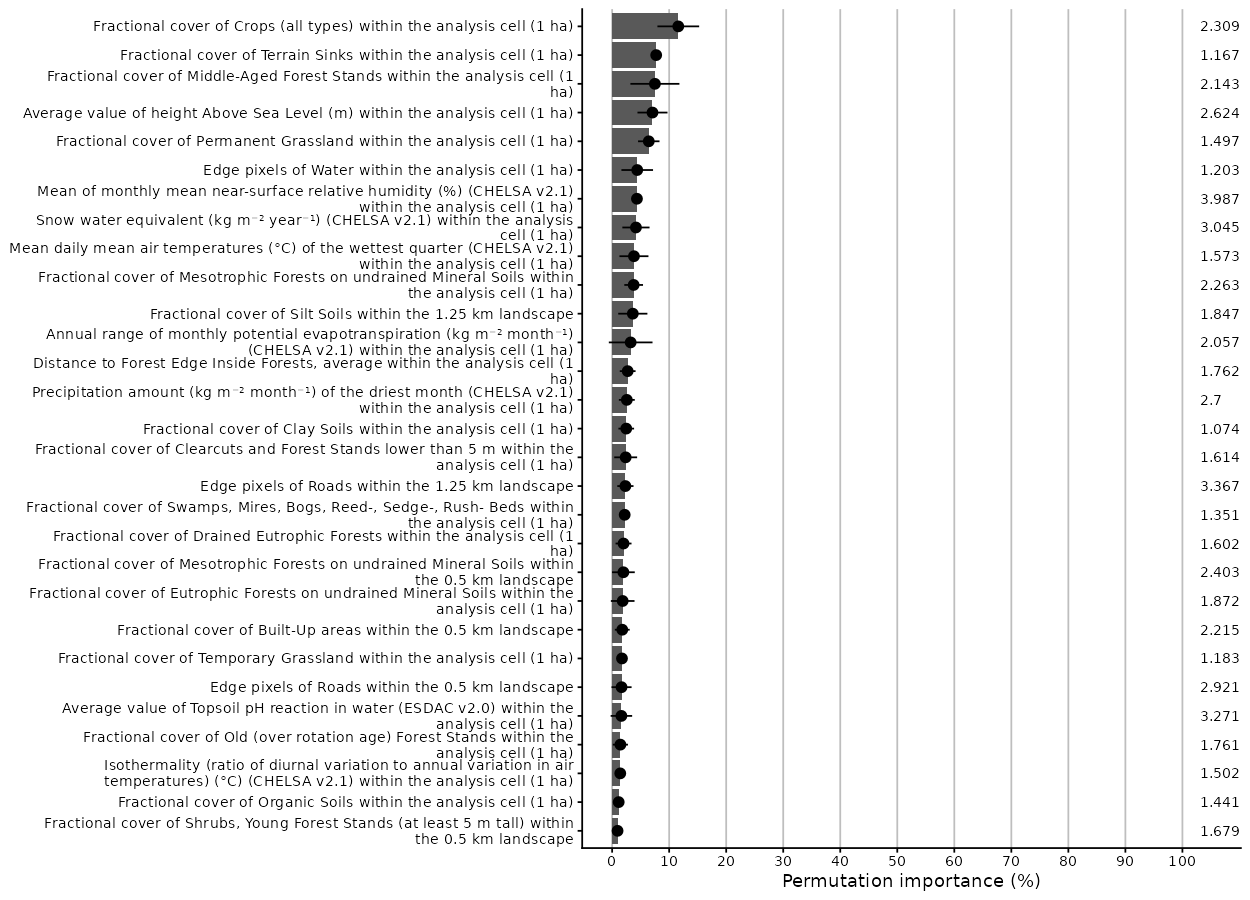
\includegraphics[width=1\linewidth,height=0.70\textheight,keepaspectratio]{results/PELFUSv2b/PicVarImpVIFs_PELFUS.png}

\par\small\textit{Permutation-importance (mean and standard deviation from 99 permutations, on the x-axis) of the ecogeographical variables (first y-axis, left side), and their variance inflation factor values (second y-axis, right side). **For a full resolution refer to repository: link or online document: link**}\normalsize
\end{center}

\section*{Marginal responses}\label{marginal-responses-7}
\addcontentsline{toc}{section}{Marginal responses}

\begin{center}
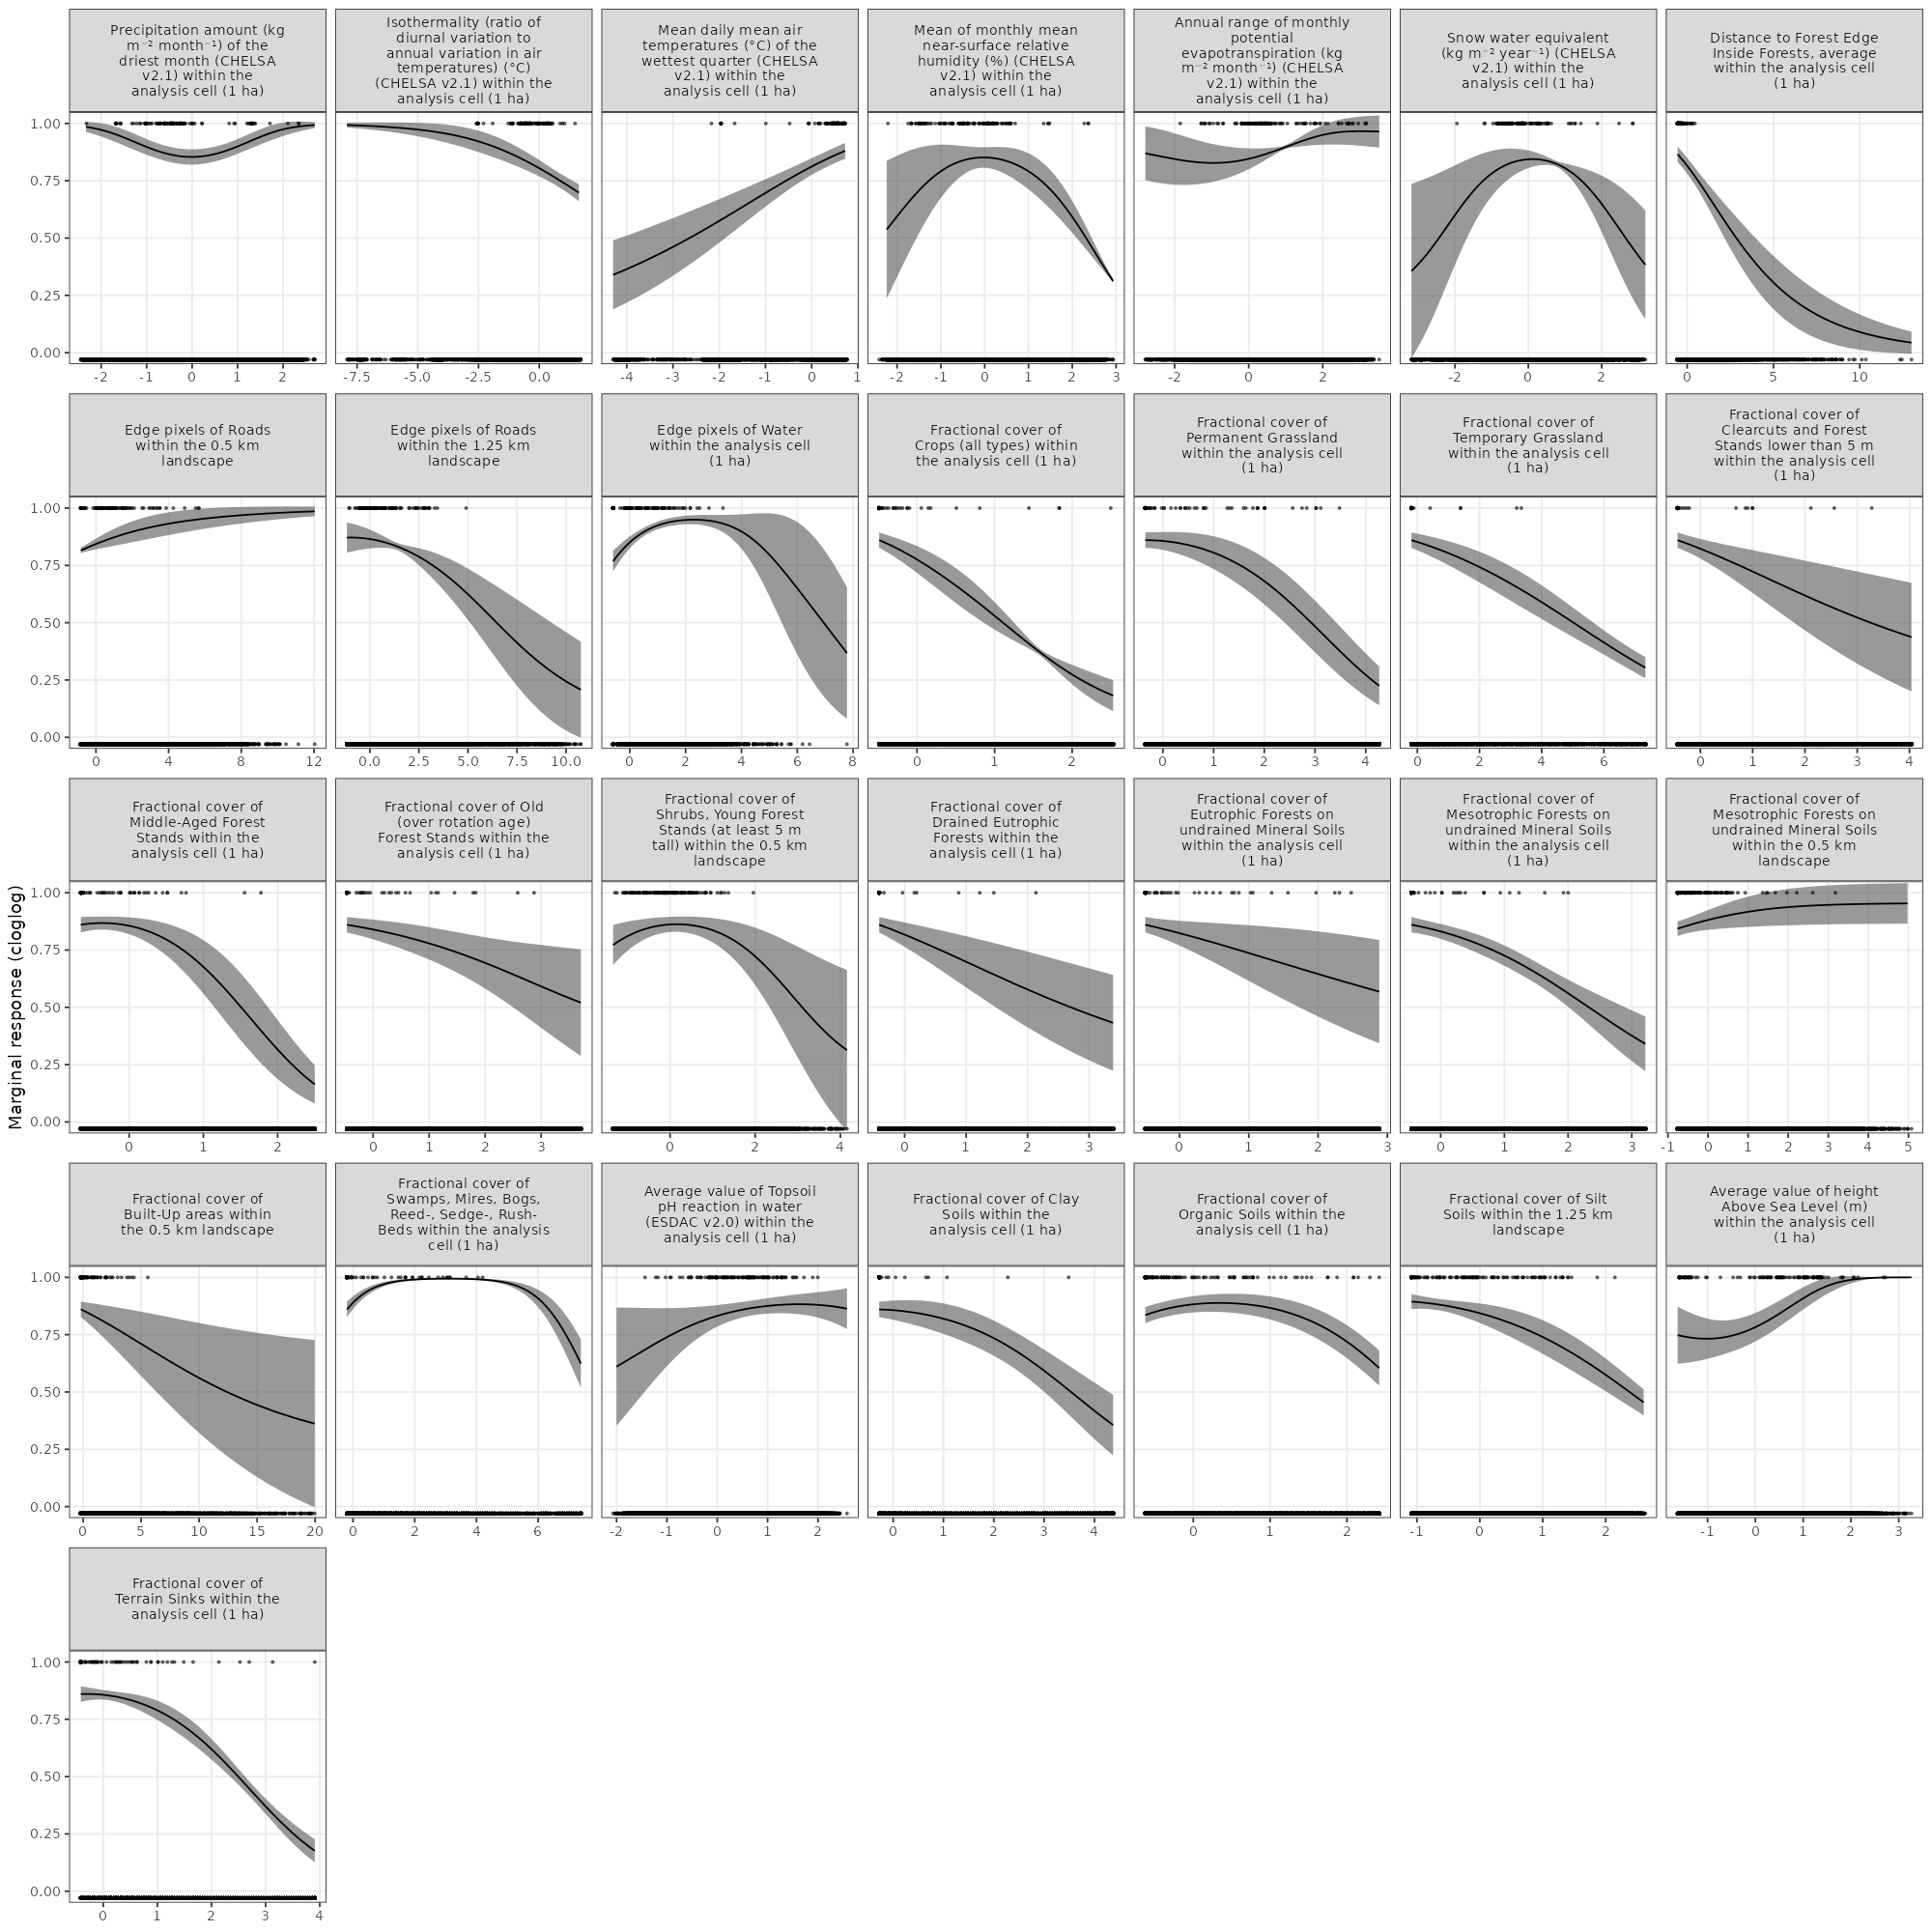
\includegraphics[width=1\linewidth,height=0.70\textheight,keepaspectratio]{results/PELFUSv2b/PicMargResp_PELFUS.png}

\par\small\textit{Marginalised for arithmetic mean response curves illustrating the effect of each ecogeographical variable on the habitat suitability when all the other variables have their arithmetic mean values. The y-axis shows the predicted habitat suitability (cloglog-transformed), while the x-axis shows the standardised (centred and scaled) value of the ecogeographical variable. Dots at a value of 1 on the y-axis illustrate presence locations in the environment (on the x-axis), while dots at a value of 0 illustrate background locations used in modelling.  **For a full resolution refer to repository: link or online document: link**}\normalsize
\end{center}

\section*{Habitat and conservation associations}\label{habitat-and-conservation-associations-7}
\addcontentsline{toc}{section}{Habitat and conservation associations}

\begin{center}
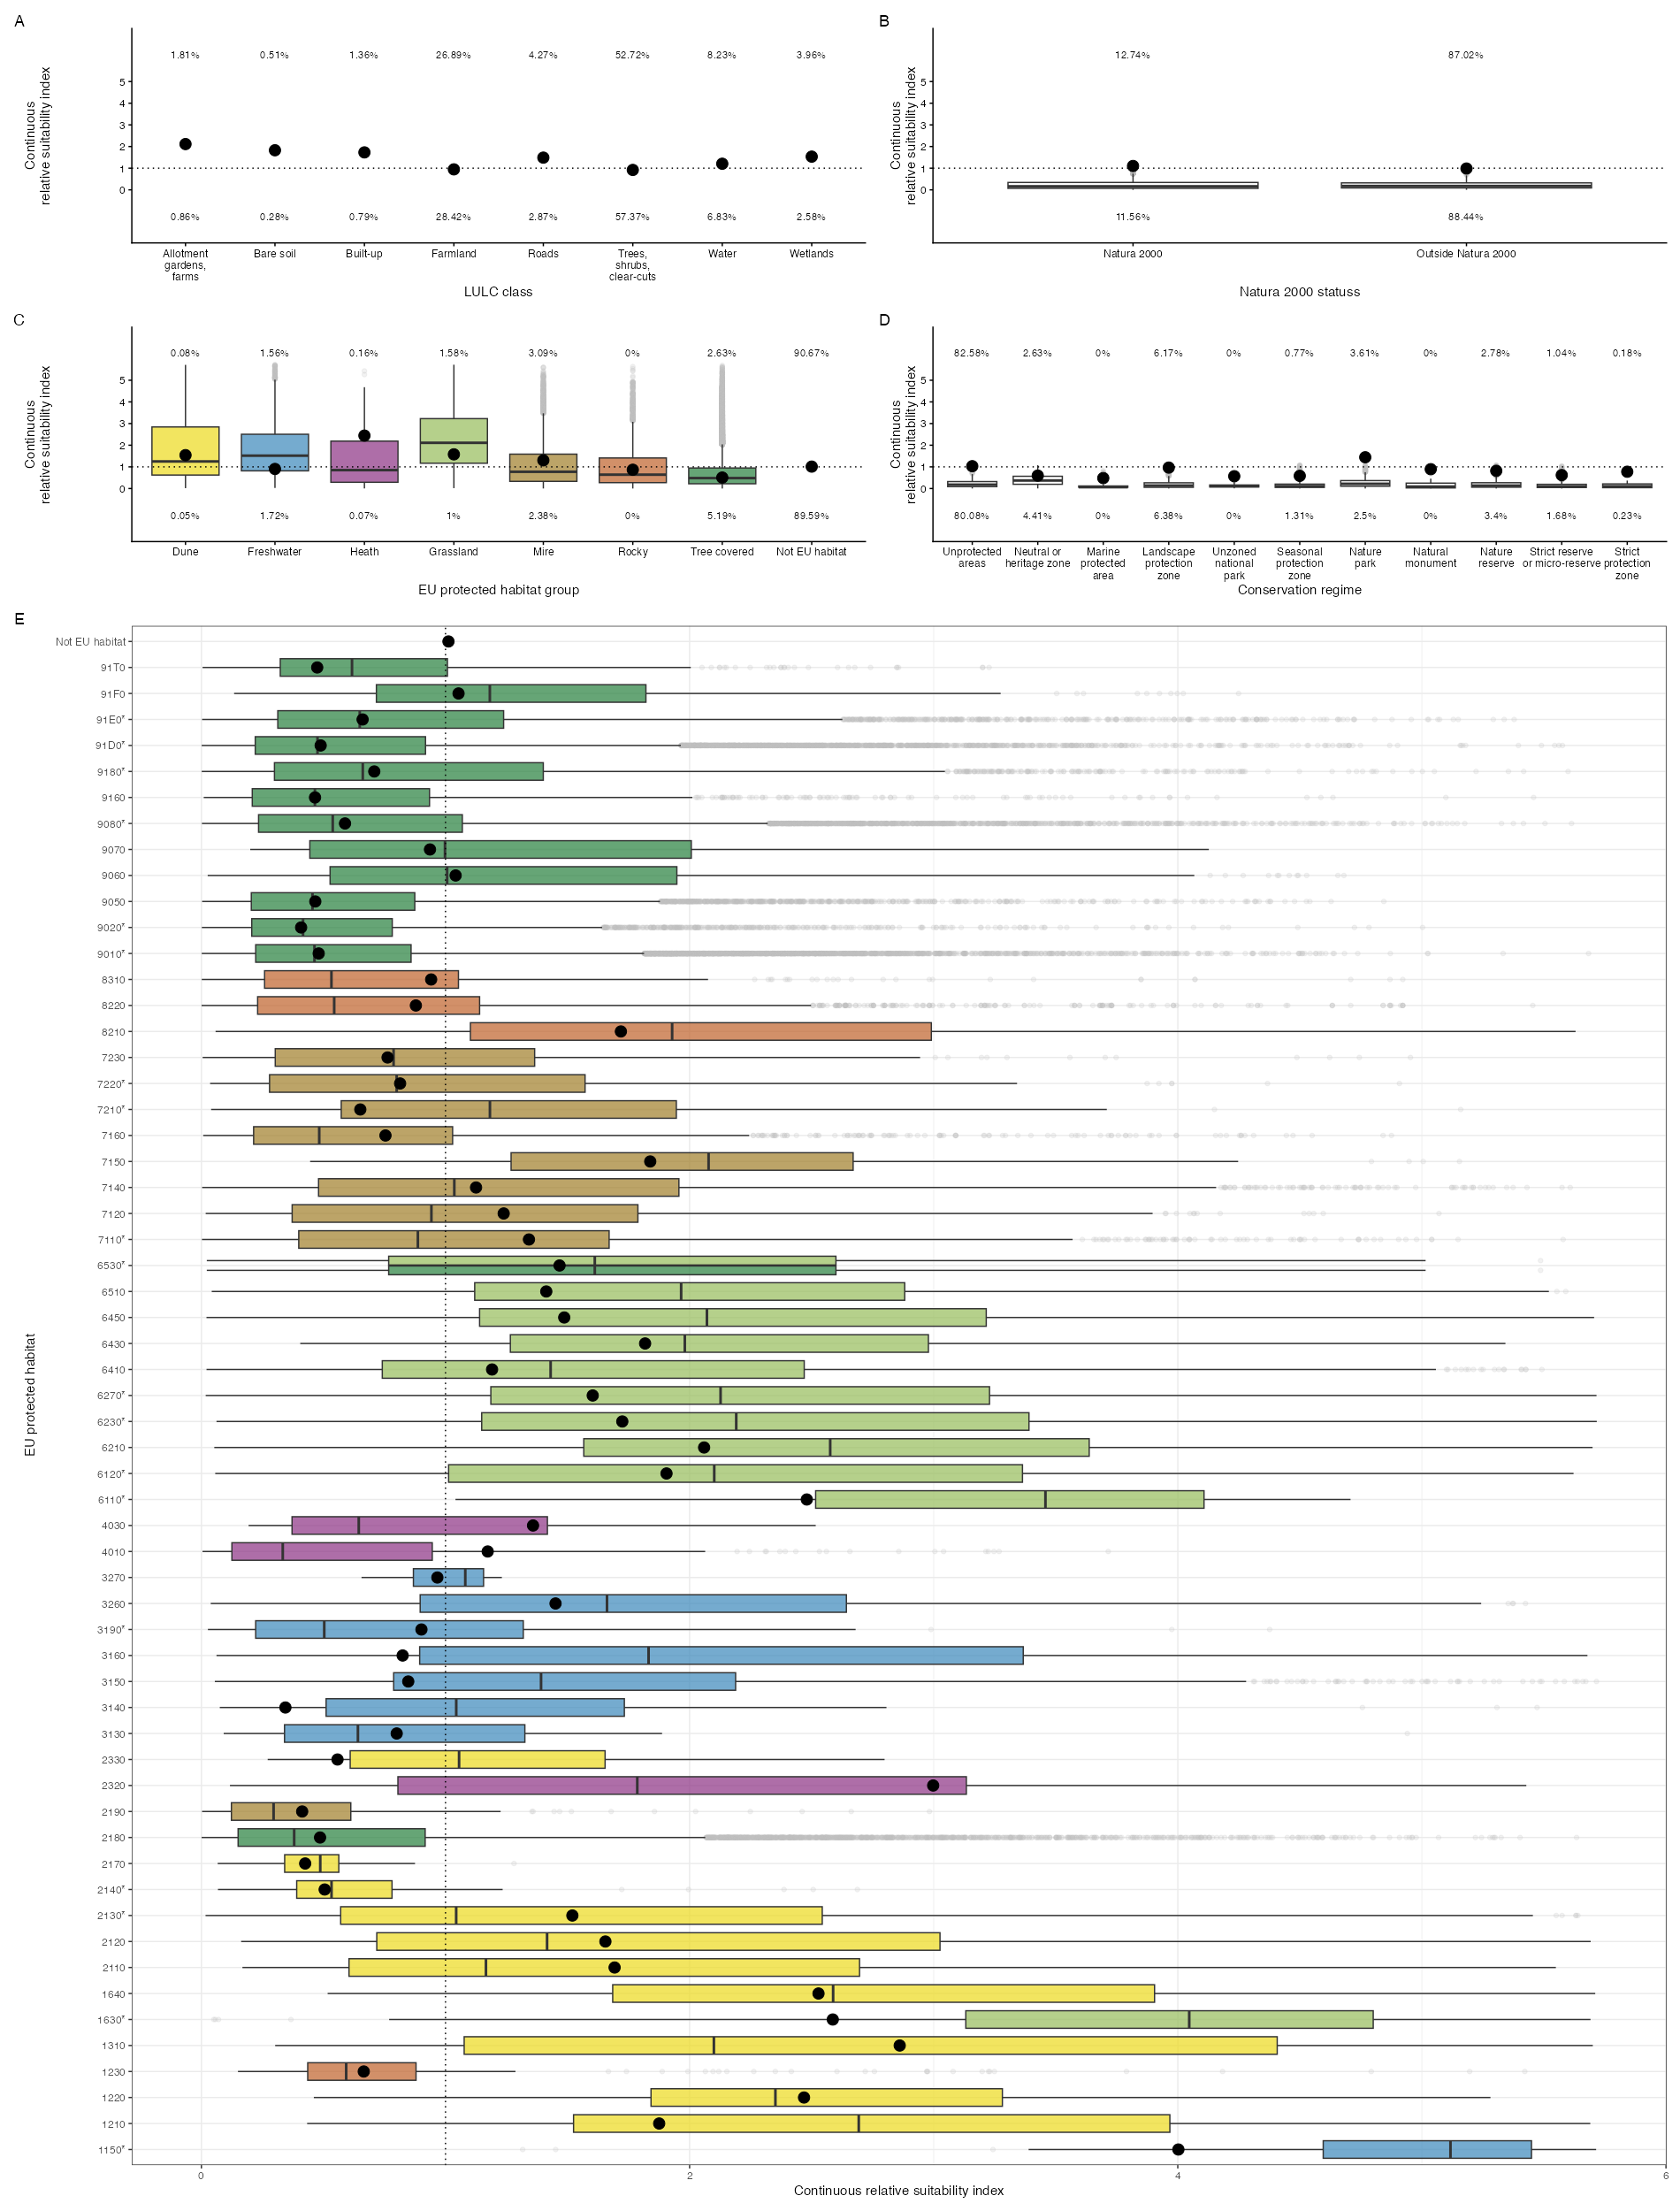
\includegraphics[width=1\linewidth,height=0.70\textheight,keepaspectratio]{results/PELFUSv2b/PicAssoc_PELFUS.png}

\par\small\textit{Associations between predicted suitability and: (A) land use land cover classes, (B) Natura 2000 status, (C) stratified EU protected habitat classes, (D) conservation regime, and (E) EU protected habitats. The y-axis show continuous relative suitability index (derivative of Manly's index of preference). Colours in (C) and (E) correspond to stratified EU protected habitat classes. For classifications composed of multiple individual polygons, polygon-level indices were additionally calculated to show within-category variation. The figures therefore combine category-level estimates (points) with the distributions of polygon-level values (boxplots, where applicable). Labels above and below the panels report, respectively, the percentage of total predicted suitability and the percentage of mapped area represented by each category. **For a full resolution refer to repository: link or online document: link**}\normalsize
\end{center}

\section*{Conservation prioritization}\label{conservation-prioritization-7}
\addcontentsline{toc}{section}{Conservation prioritization}

\begin{center}
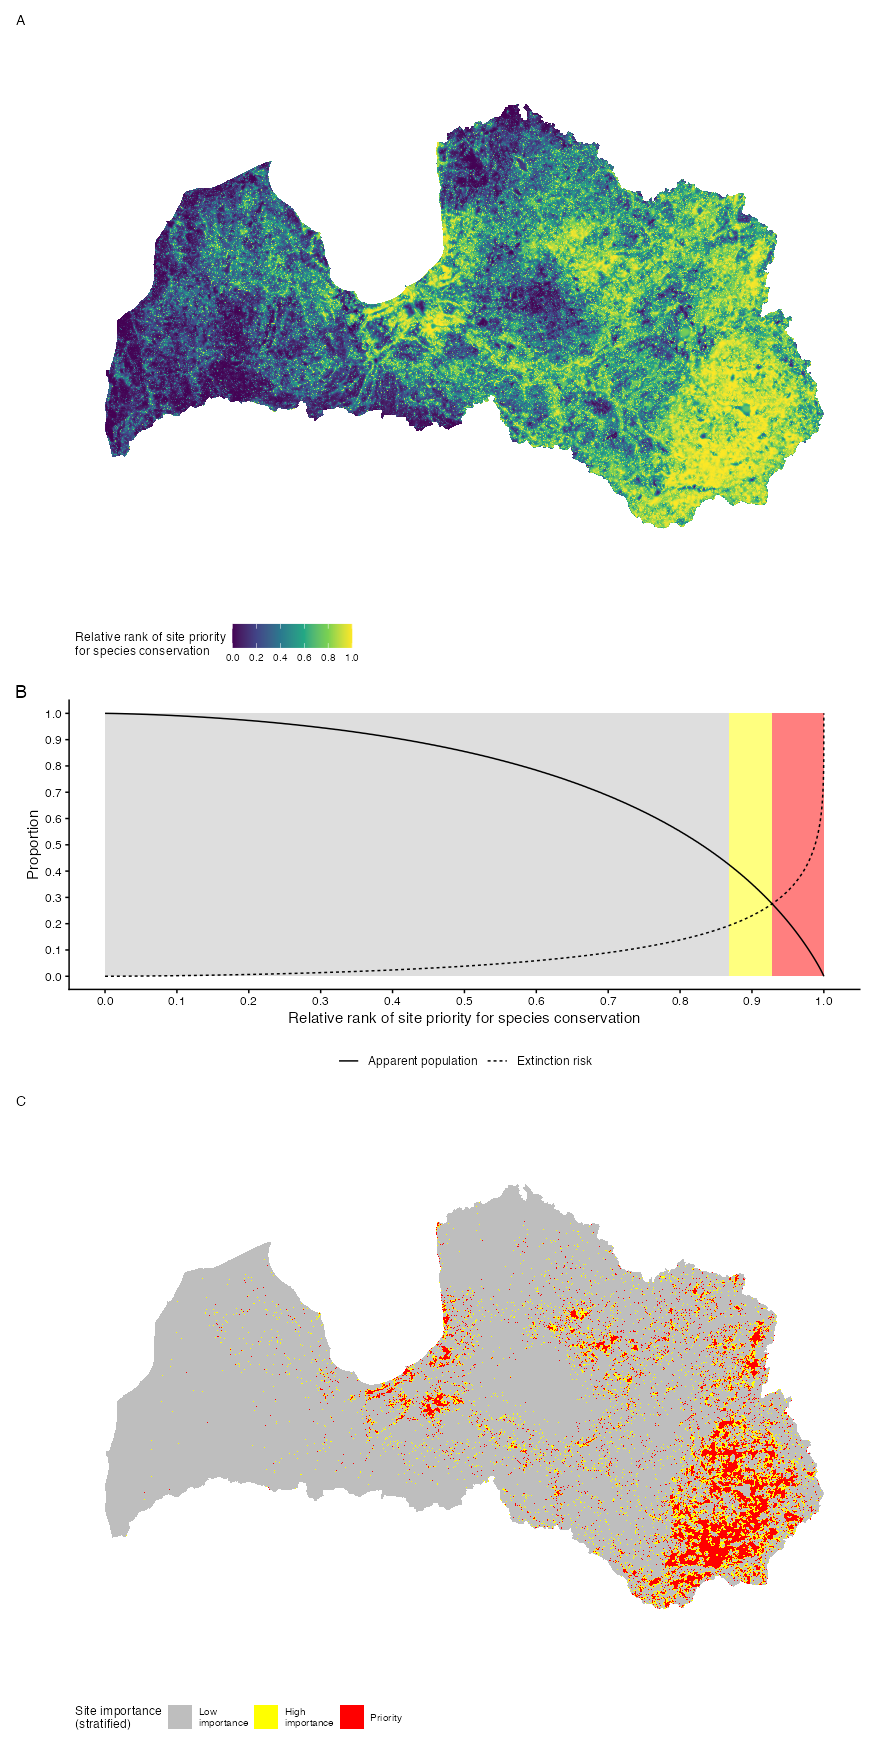
\includegraphics[width=0.85\linewidth,height=0.70\textheight,keepaspectratio]{results/PELFUSv2b/PicPrior_PELFUS.png}

\par\small\textit{Single-species conservation prioritization focusing on maximisation of core area protection (CAZMAX) while accounting for site connectivity: (A) relative site rank; (B) relationship between apparent-population and extinction-risk curves with a simplified classification which is spatially demonstrated in the bootom row; (C) spatial distribution of proposed classification of site prioritization results. **For a full resolution refer to repository: link or online document: link**}\normalsize
\end{center}

\chapter*{\texorpdfstring{\emph{Pelobates fuscus} monitoring}{Pelobates fuscus monitoring}}\label{pelfusmonitoring}
\addcontentsline{toc}{chapter}{\emph{Pelobates fuscus} monitoring}

\section*{Summary}\label{summary-8}
\addcontentsline{toc}{section}{Summary}

\subsection*{Model description}\label{model-description-8}
\addcontentsline{toc}{subsection}{Model description}

Occurrence and background data were divided into model-training with four block spatial cross-validation data and an independent test set. Sampling-bias/background treatment: \textbf{Phenology Weighted Target Group}. Accumulated LULC change within the 1-ha analysis cell was not evaluated; accumulated LULC change within the home-range radius around the analysis cell was not evaluated.

The final data set contained \textbf{138} presence records: \textbf{104} for training with four spatial block cross-validation and \textbf{34} for independent testing. Training background contained \textbf{30146} locations, with \textbf{9854} additional independent-test background locations.

\subsection*{Expert assessment scores}\label{expert-assessment-scores-8}
\addcontentsline{toc}{subsection}{Expert assessment scores}

\begin{itemize}
\tightlist
\item
  \textbf{Marginal responses and variable importance score:} 4 (good ecological interpretability)
\item
  \textbf{Map score:} 1 (poor agreement with known distribution)
\item
  \textbf{Applicability score:} 1 (very limited applicability)
\end{itemize}

\textbf{Šo sadaļu aizpildām manuāli no ekspertu aptaujām}

\subsection*{Statistical evaluation}\label{statistical-evaluation-8}
\addcontentsline{toc}{subsection}{Statistical evaluation}

The final model had a training TSS of \textbf{0.401}, with a training-derived cloglog threshold of \textbf{0.617}. Combined training AUC was \textbf{0.839} and combined test AUC was \textbf{0.724}.

\subsubsection*{Spatial cross-validation}\label{spatial-cross-validation-8}
\addcontentsline{toc}{subsubsection}{Spatial cross-validation}

\begin{itemize}
\tightlist
\item
  \textbf{AUC:} 0.7759 ± 0.0111; null models: 0.5248 ± 0.0256; z = 9.8265, p \textless{} 0.001
\item
  \textbf{CBI:} 0.8578 ± 0.0478; null models: 0.0488 ± 0.1284; z = 6.2992, p \textless{} 0.001
\item
  \textbf{OR10:} 0.1058 ± 0.0484; null models: 0.0531 ± 0.0662; z = 0.7956, p = 0.787
\item
  \textbf{ORmin:} 0 ± 0; null models: 0.0066 ± 0.0289; z = -0.2296, p = 0.409
\end{itemize}

\subsubsection*{Independent testing}\label{independent-testing-8}
\addcontentsline{toc}{subsubsection}{Independent testing}

\begin{itemize}
\tightlist
\item
  \textbf{TSS:} 0.264; \textbf{sensitivity:} 0.441; \textbf{specificity:} 0.823
\item
  \textbf{AUC:} 0.716; null models: 0.4944 ± 0.0819; z = 2.7033, p = 0.003
\item
  \textbf{CBI:} 0.791; null models: 0.002 ± 0.4027; z = 1.9591, p = 0.025
\item
  \textbf{OR10:} 0.206; null models: 0.1194 ± 0.1032; z = 0.8376, p = 0.799
\item
  \textbf{ORmin:} 0; null models: 0.0062 ± 0.0179; z = -0.3454, p = 0.365
\end{itemize}

\subsection*{Conservation prioritisation summary}\label{conservation-prioritisation-summary-8}
\addcontentsline{toc}{subsection}{Conservation prioritisation summary}

The primary priority area covers \textbf{10.5\%} of Latvia and contains \textbf{27.6\%} of the summed habitat suitability (apparent population proxy).

The broader high importance area covers \textbf{14.4\%} of Latvia and contains \textbf{35.2\%} of the summed habitat suitability.

For comparison, the area classified as suitable using the maximum training sensitivity plus specificity habitat-suitability threshold contains \textbf{35.2\%} of the summed continuous habitat suitability.

\subsection*{Version evolution}\label{version-evolution-8}
\addcontentsline{toc}{subsection}{Version evolution}

\textbf{Šo sadaļu aizpildām manuāli, izmntojot sagatavotās shēmas. Jāvienojas par to noformējumu}

\section*{Habitat suitability}\label{habitat-suitability-8}
\addcontentsline{toc}{section}{Habitat suitability}

\begin{center}
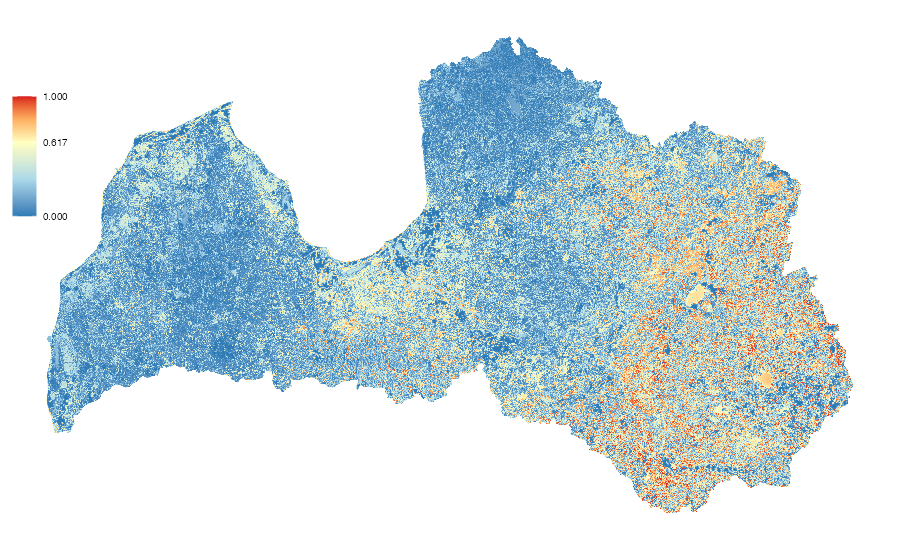
\includegraphics[width=1\linewidth,height=0.70\textheight,keepaspectratio]{results/PELFUSmonitoring_v2b5/PicHSmap_PELFUSmonitoring.png}

\par\small\textit{Predicted continuous habitat suitability across Latvia. The warmer the colour the higher is the predicted habitat suitability. Value in the middle of the legend correspond to the maximum training sensitivity plus specificity threshold. **For a full resolution refer to repository: link or online document: link**}\normalsize
\end{center}

\section*{Model thresholds}\label{model-thresholds-8}
\addcontentsline{toc}{section}{Model thresholds}

Threshold values and associated omission rates

\begin{center}
\resizebox{\linewidth}{!}{%

\begin{tabular}{lrrrrr}
\toprule
Threshold & Cloglog value & Fractional predicted area & Training omission rate & Test omission rate & P-values\\
\midrule
Minimum training presence & 0.0826184 & 0.8440422 & 0.0000000 & 0.0000000 & 0\\
Equal training sensitivity and specificity & 0.5595000 & 0.2403687 & 0.2403846 & 0.0017182 & 0\\
Maximum training sensitivity plus specificity & 0.6167279 & 0.1953783 & 0.2596154 & 0.0019204 & 0\\
Equal test sensitivity and specificity & 0.4361591 & 0.3553146 & 0.1538462 & 0.0012129 & 0\\
Maximum test sensitivity plus specificity & 0.3980361 & 0.3948346 & 0.1057692 & 0.0007075 & 0\\
\bottomrule
\end{tabular}
}
\end{center}

\section*{Variable importance}\label{variable-importance-8}
\addcontentsline{toc}{section}{Variable importance}

\begin{center}
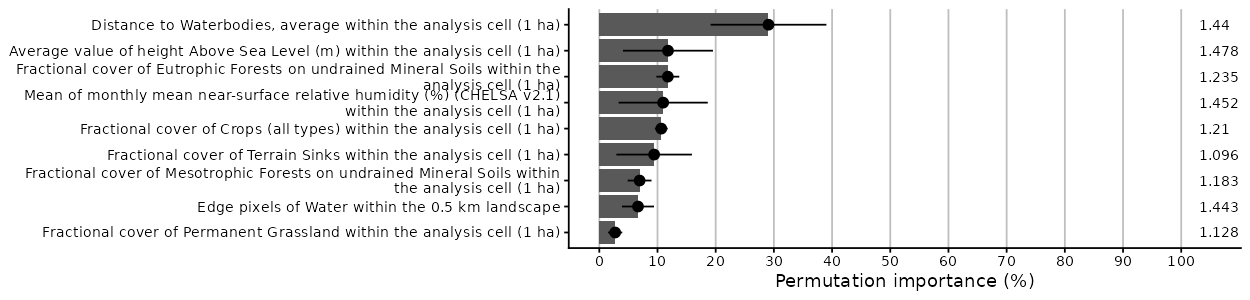
\includegraphics[width=1\linewidth,height=0.70\textheight,keepaspectratio]{results/PELFUSmonitoring_v2b5/PicVarImpVIFs_PELFUSmonitoring.png}

\par\small\textit{Permutation-importance (mean and standard deviation from 99 permutations, on the x-axis) of the ecogeographical variables (first y-axis, left side), and their variance inflation factor values (second y-axis, right side). **For a full resolution refer to repository: link or online document: link**}\normalsize
\end{center}

\section*{Marginal responses}\label{marginal-responses-8}
\addcontentsline{toc}{section}{Marginal responses}

\begin{center}
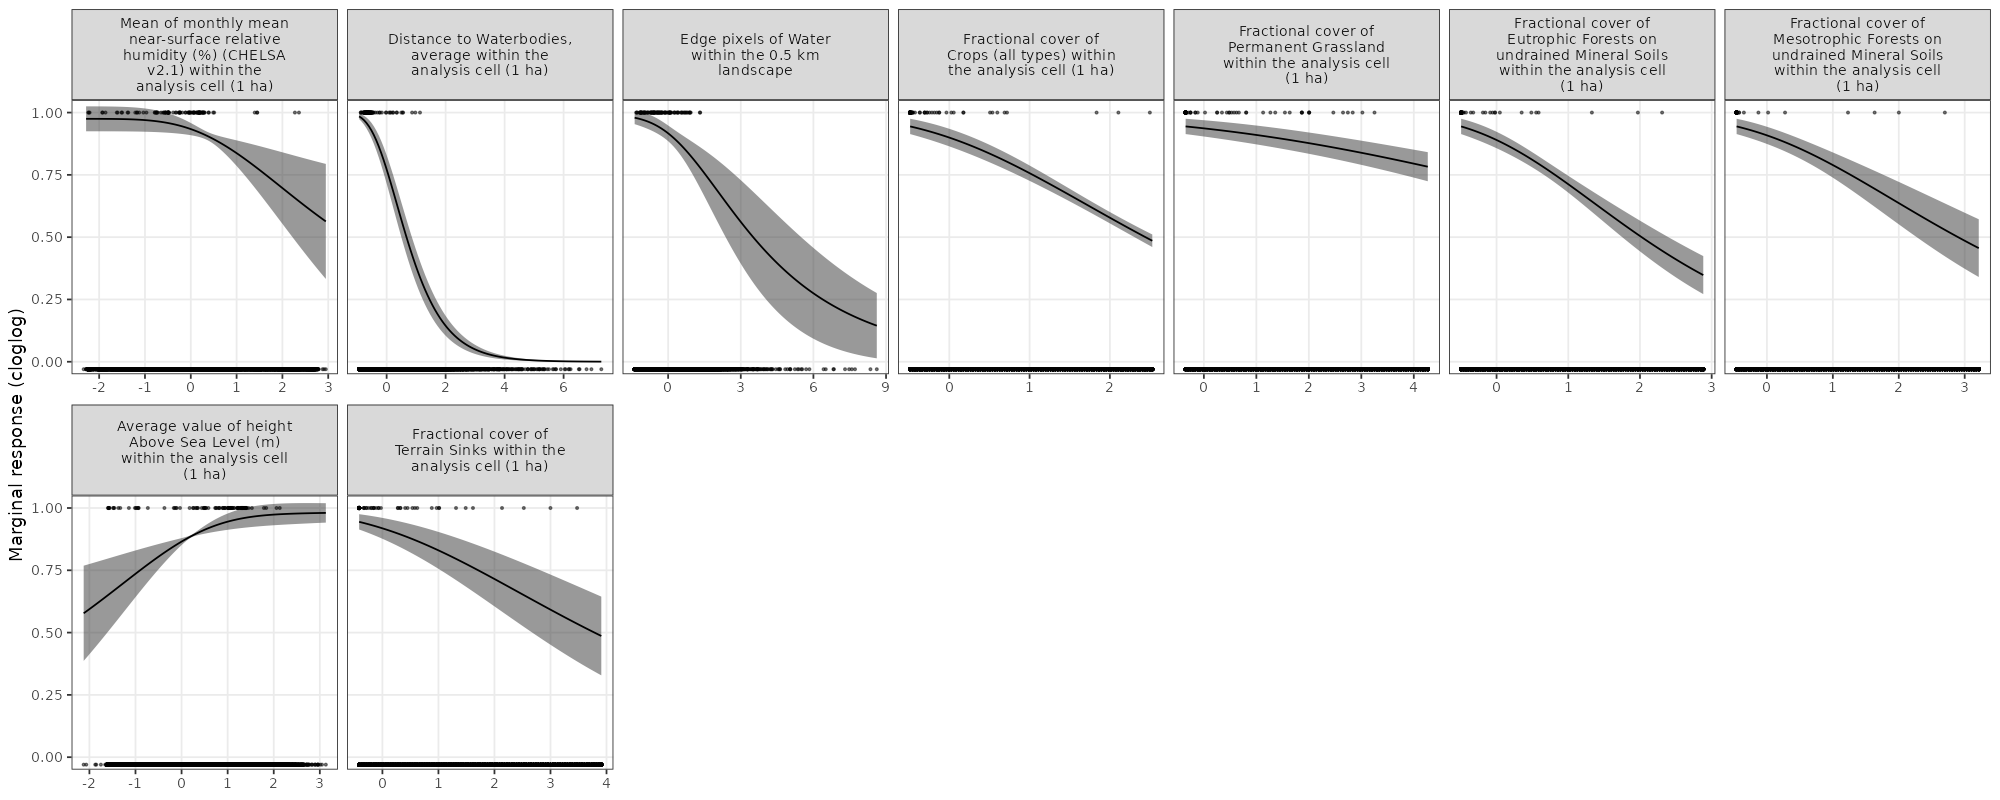
\includegraphics[width=1\linewidth,height=0.70\textheight,keepaspectratio]{results/PELFUSmonitoring_v2b5/PicMargResp_PELFUSmonitoring.png}

\par\small\textit{Marginalised for arithmetic mean response curves illustrating the effect of each ecogeographical variable on the habitat suitability when all the other variables have their arithmetic mean values. The y-axis shows the predicted habitat suitability (cloglog-transformed), while the x-axis shows the standardised (centred and scaled) value of the ecogeographical variable. Dots at a value of 1 on the y-axis illustrate presence locations in the environment (on the x-axis), while dots at a value of 0 illustrate background locations used in modelling.  **For a full resolution refer to repository: link or online document: link**}\normalsize
\end{center}

\section*{Habitat and conservation associations}\label{habitat-and-conservation-associations-8}
\addcontentsline{toc}{section}{Habitat and conservation associations}

\begin{center}
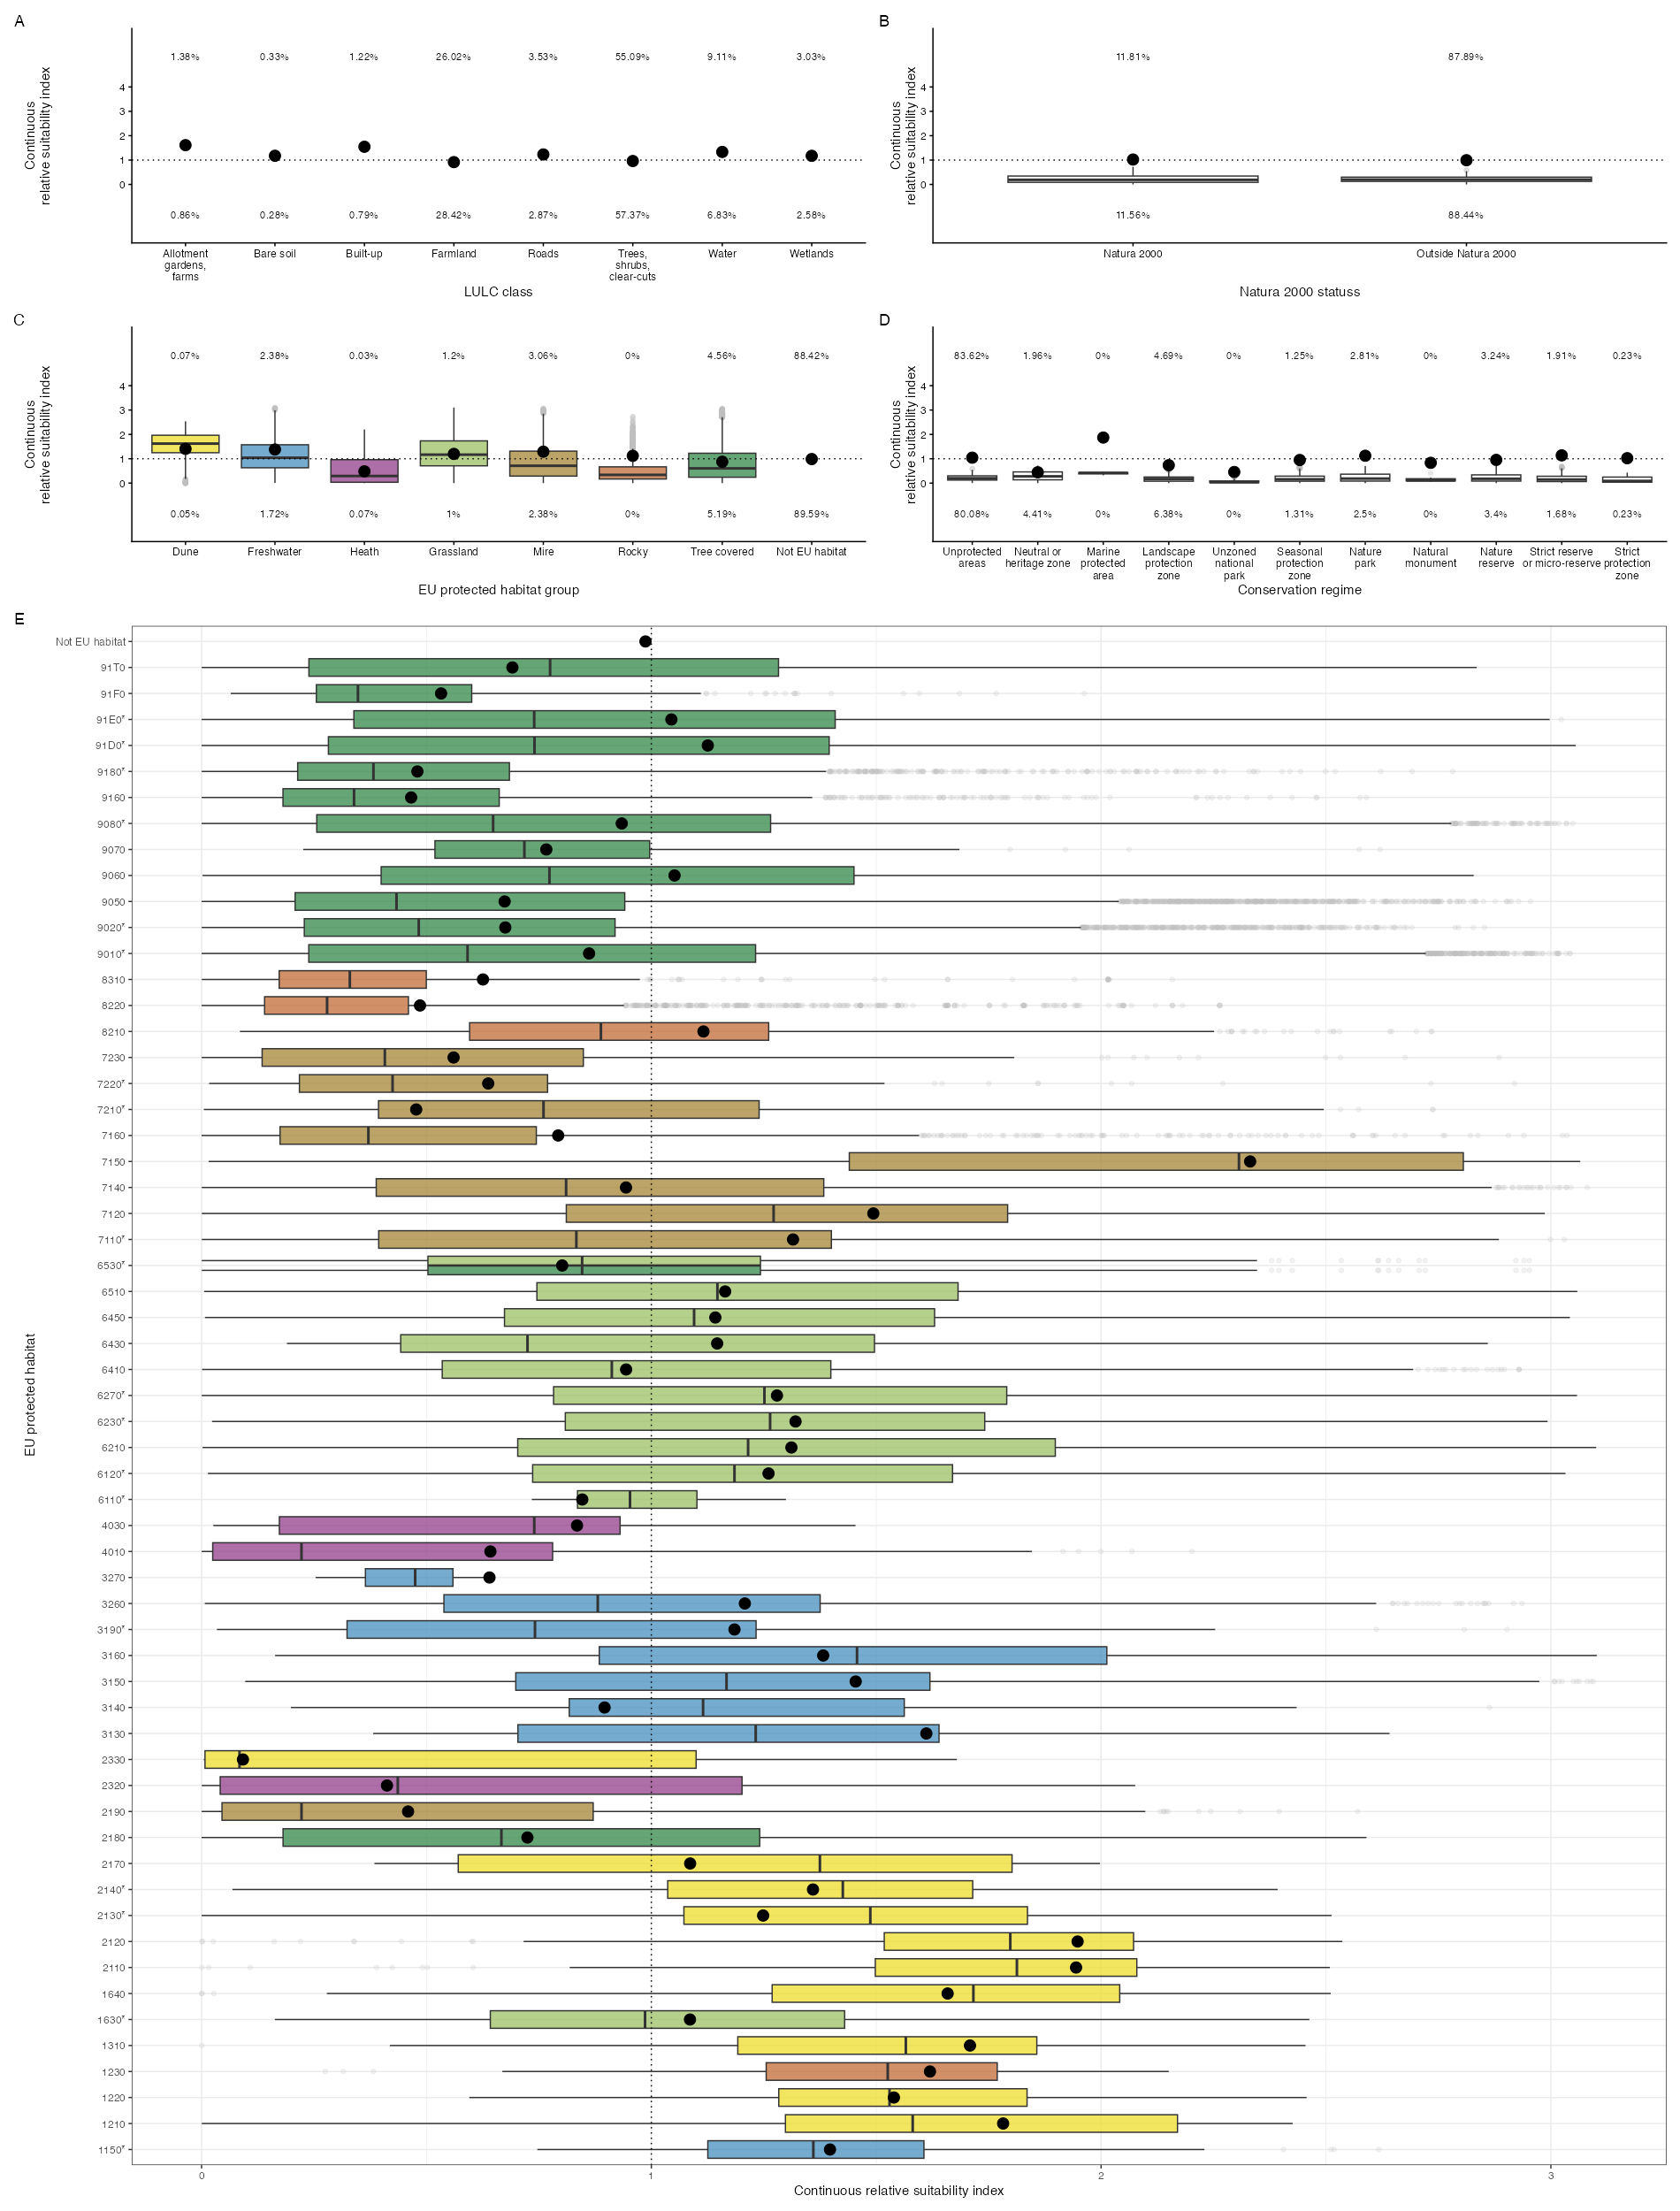
\includegraphics[width=1\linewidth,height=0.70\textheight,keepaspectratio]{results/PELFUSmonitoring_v2b5/PicAssoc_PELFUSmonitoring.png}

\par\small\textit{Associations between predicted suitability and: (A) land use land cover classes, (B) Natura 2000 status, (C) stratified EU protected habitat classes, (D) conservation regime, and (E) EU protected habitats. The y-axis show continuous relative suitability index (derivative of Manly's index of preference). Colours in (C) and (E) correspond to stratified EU protected habitat classes. For classifications composed of multiple individual polygons, polygon-level indices were additionally calculated to show within-category variation. The figures therefore combine category-level estimates (points) with the distributions of polygon-level values (boxplots, where applicable). Labels above and below the panels report, respectively, the percentage of total predicted suitability and the percentage of mapped area represented by each category. **For a full resolution refer to repository: link or online document: link**}\normalsize
\end{center}

\section*{Conservation prioritization}\label{conservation-prioritization-8}
\addcontentsline{toc}{section}{Conservation prioritization}

\begin{center}
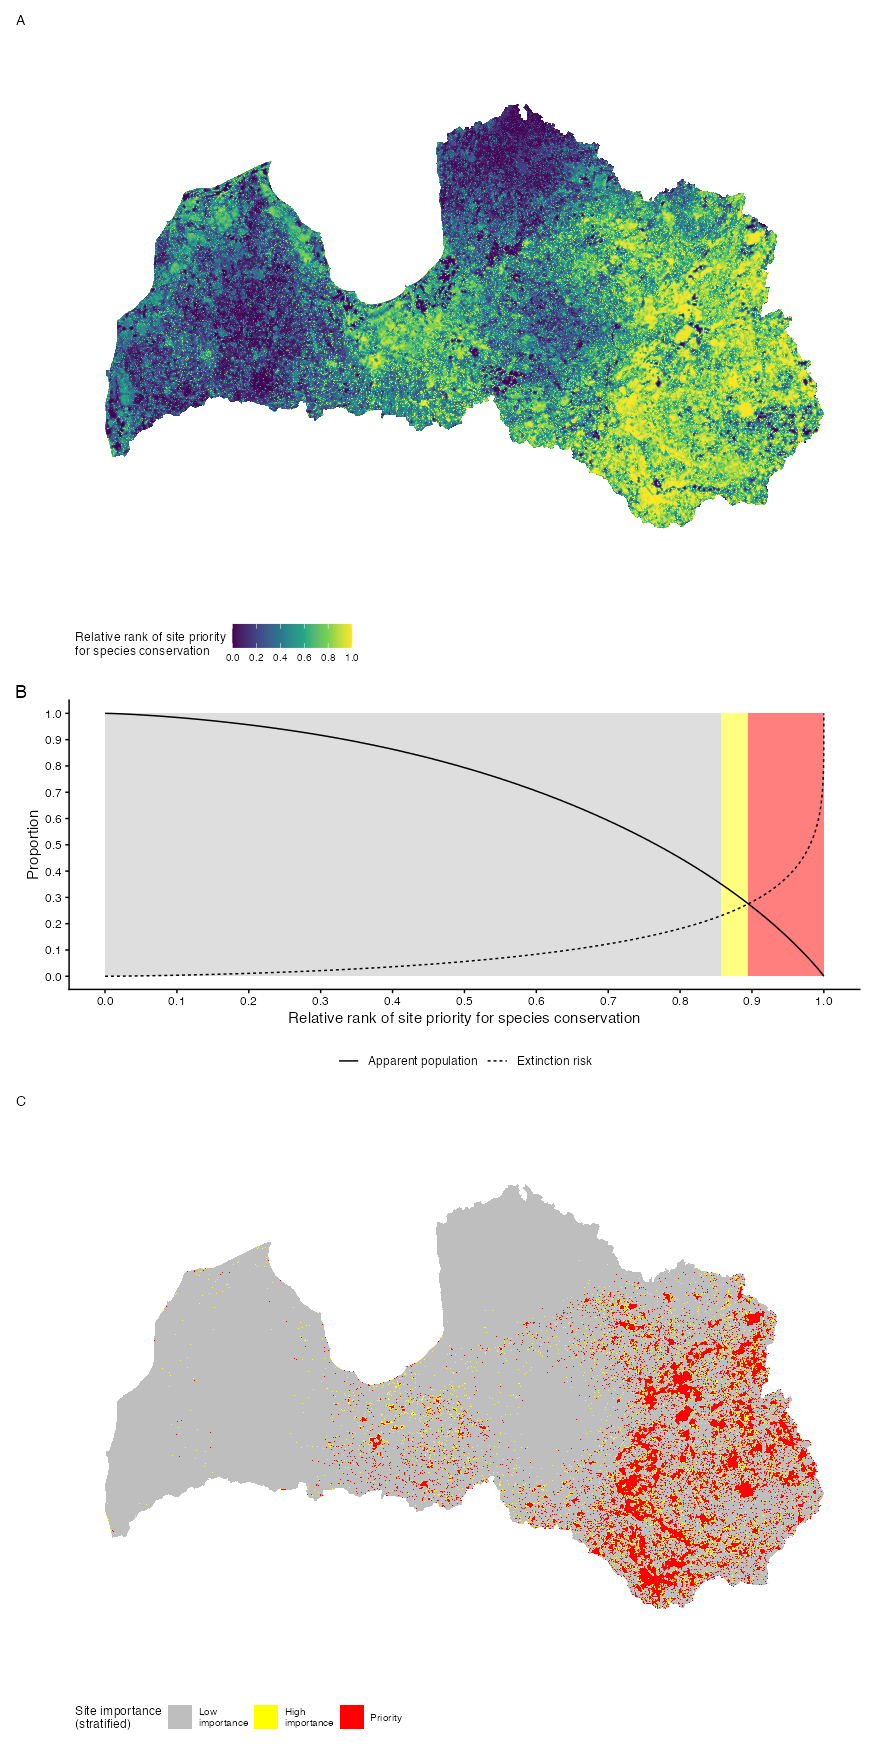
\includegraphics[width=0.85\linewidth,height=0.70\textheight,keepaspectratio]{results/PELFUSmonitoring_v2b5/PicPrior_PELFUSmonitoring.png}

\par\small\textit{Single-species conservation prioritization focusing on maximisation of core area protection (CAZMAX) while accounting for site connectivity: (A) relative site rank; (B) relationship between apparent-population and extinction-risk curves with a simplified classification which is spatially demonstrated in the bootom row; (C) spatial distribution of proposed classification of site prioritization results. **For a full resolution refer to repository: link or online document: link**}\normalsize
\end{center}

\chapter*{\texorpdfstring{\emph{Bufo bufo}}{Bufo bufo}}\label{bufbuf}
\addcontentsline{toc}{chapter}{\emph{Bufo bufo}}

\section*{Summary}\label{summary-9}
\addcontentsline{toc}{section}{Summary}

\subsection*{Model description}\label{model-description-9}
\addcontentsline{toc}{subsection}{Model description}

Occurrence and background data were divided into model-training with four block spatial cross-validation data and an independent test set. Sampling-bias/background treatment: \textbf{Phenology Weighted Target Group}. Accumulated LULC change within the 1-ha analysis cell was not evaluated; accumulated LULC change within the home-range radius around the analysis cell was not evaluated.

The final data set contained \textbf{560} presence records: \textbf{420} for training with four spatial block cross-validation and \textbf{140} for independent testing. Training background contained \textbf{30002} locations, with \textbf{9998} additional independent-test background locations.

\subsection*{Expert assessment scores}\label{expert-assessment-scores-9}
\addcontentsline{toc}{subsection}{Expert assessment scores}

\begin{itemize}
\tightlist
\item
  \textbf{Marginal responses and variable importance score:} 4 (good ecological interpretability)
\item
  \textbf{Map score:} 3 (moderate agreement with known distribution)
\item
  \textbf{Applicability score:} 3 (moderate applicability)
\end{itemize}

\textbf{Šo sadaļu aizpildām manuāli no ekspertu aptaujām}

\subsection*{Statistical evaluation}\label{statistical-evaluation-9}
\addcontentsline{toc}{subsection}{Statistical evaluation}

The final model had a training TSS of \textbf{0.401}, with a training-derived cloglog threshold of \textbf{0.529}. Combined training AUC was \textbf{0.757} and combined test AUC was \textbf{0.751}.

\subsubsection*{Spatial cross-validation}\label{spatial-cross-validation-9}
\addcontentsline{toc}{subsubsection}{Spatial cross-validation}

\begin{itemize}
\tightlist
\item
  \textbf{AUC:} 0.7298 ± 0.0425; null models: 0.5487 ± 0.0239; z = 7.5834, p \textless{} 0.001
\item
  \textbf{CBI:} 0.913 ± 0.0562; null models: 0.3403 ± 0.1838; z = 3.1161, p = 0.001
\item
  \textbf{OR10:} 0.1238 ± 0.0544; null models: 0.126 ± 0.0515; z = -0.0434, p = 0.483
\item
  \textbf{ORmin:} 0.0024 ± 0.0048; null models: 0.0071 ± 0.0156; z = -0.3029, p = 0.381
\end{itemize}

\subsubsection*{Independent testing}\label{independent-testing-9}
\addcontentsline{toc}{subsubsection}{Independent testing}

\begin{itemize}
\tightlist
\item
  \textbf{TSS:} 0.339; \textbf{sensitivity:} 0.629; \textbf{specificity:} 0.71
\item
  \textbf{AUC:} 0.747; null models: 0.5112 ± 0.0697; z = 3.3821, p \textless{} 0.001
\item
  \textbf{CBI:} 0.99; null models: 0.0623 ± 0.5101; z = 1.8186, p = 0.034
\item
  \textbf{OR10:} 0.107; null models: 0.133 ± 0.0644; z = -0.4017, p = 0.344
\item
  \textbf{ORmin:} 0; null models: 0.0019 ± 0.0045; z = -0.4263, p = 0.335
\end{itemize}

\subsection*{Conservation prioritisation summary}\label{conservation-prioritisation-summary-9}
\addcontentsline{toc}{subsection}{Conservation prioritisation summary}

The primary priority area covers \textbf{13.4\%} of Latvia and contains \textbf{27.6\%} of the summed habitat suitability (apparent population proxy).

The broader high importance area covers \textbf{29.1\%} of Latvia and contains \textbf{50.5\%} of the summed habitat suitability.

For comparison, the area classified as suitable using the maximum training sensitivity plus specificity habitat-suitability threshold contains \textbf{50.5\%} of the summed continuous habitat suitability.

\subsection*{Version evolution}\label{version-evolution-9}
\addcontentsline{toc}{subsection}{Version evolution}

\textbf{Šo sadaļu aizpildām manuāli, izmntojot sagatavotās shēmas. Jāvienojas par to noformējumu}

\section*{Habitat suitability}\label{habitat-suitability-9}
\addcontentsline{toc}{section}{Habitat suitability}

\begin{center}
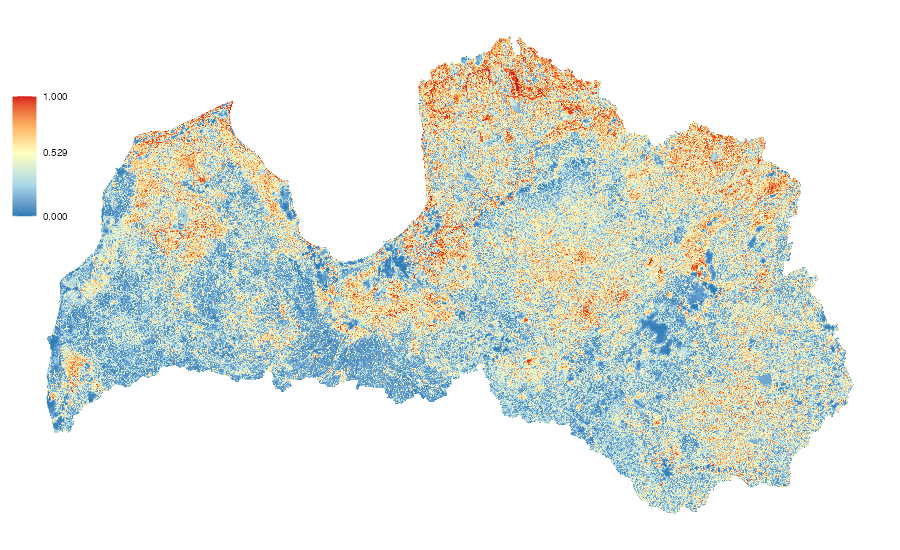
\includegraphics[width=1\linewidth,height=0.70\textheight,keepaspectratio]{results/BUFBUFv2bNM/PicHSmap_BUFBUF.png}

\par\small\textit{Predicted continuous habitat suitability across Latvia. The warmer the colour the higher is the predicted habitat suitability. Value in the middle of the legend correspond to the maximum training sensitivity plus specificity threshold. **For a full resolution refer to repository: link or online document: link**}\normalsize
\end{center}

\section*{Model thresholds}\label{model-thresholds-9}
\addcontentsline{toc}{section}{Model thresholds}

Threshold values and associated omission rates

\begin{center}
\resizebox{\linewidth}{!}{%

\begin{tabular}{lrrrrr}
\toprule
Threshold & Cloglog value & Fractional predicted area & Training omission rate & Test omission rate & P-values\\
\midrule
Minimum training presence & 0.0114637 & 0.9978889 & 0.0000000 & 0.0000000 & 0\\
Equal training sensitivity and specificity & 0.5206003 & 0.3047566 & 0.3047619 & 0.0048819 & 0\\
Maximum training sensitivity plus specificity & 0.5285540 & 0.2961802 & 0.3047619 & 0.0050771 & 0\\
Equal test sensitivity and specificity & 0.5007965 & 0.3263953 & 0.2880952 & 0.0043937 & 0\\
Maximum test sensitivity plus specificity & 0.4660263 & 0.3669020 & 0.2523810 & 0.0035149 & 0\\
\bottomrule
\end{tabular}
}
\end{center}

\section*{Variable importance}\label{variable-importance-9}
\addcontentsline{toc}{section}{Variable importance}

\begin{center}
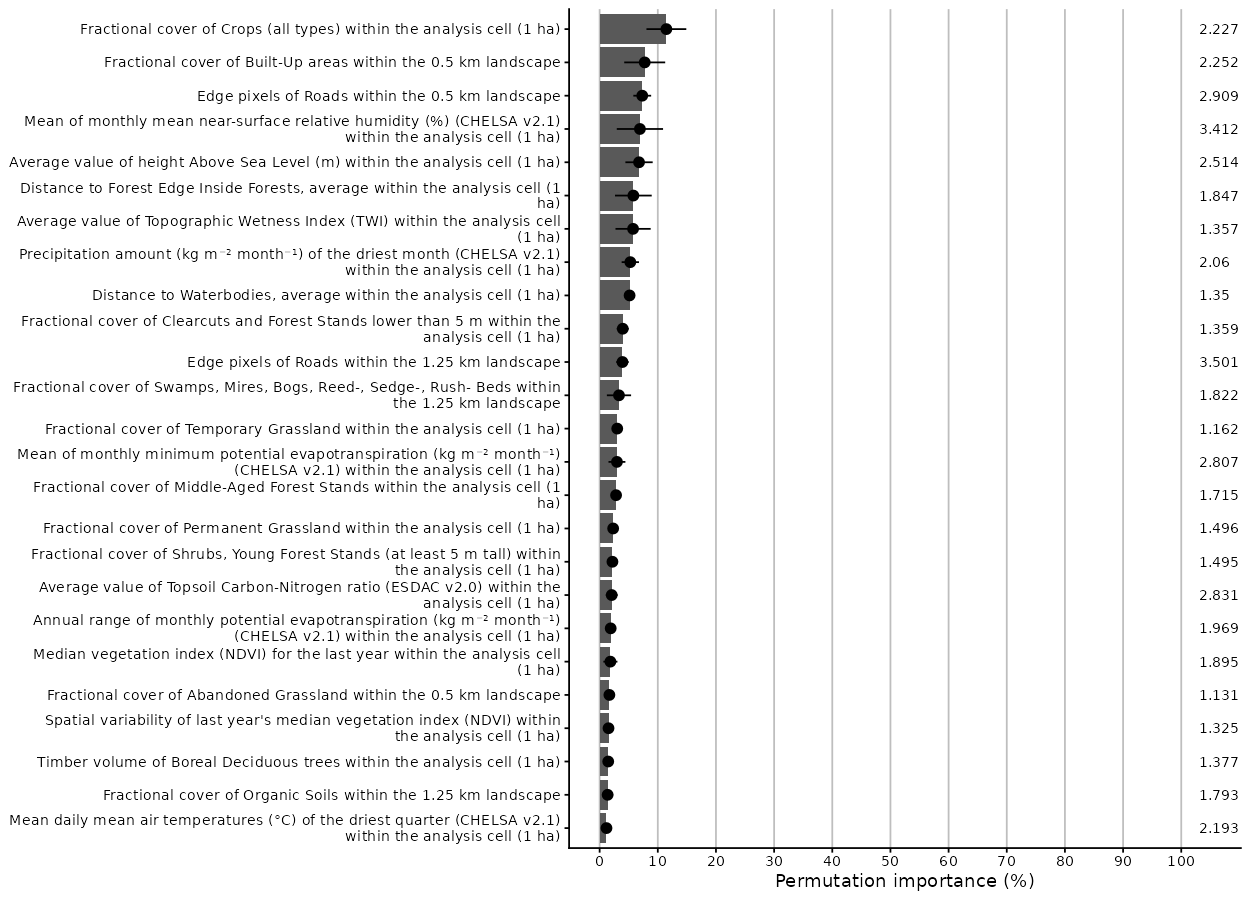
\includegraphics[width=1\linewidth,height=0.70\textheight,keepaspectratio]{results/BUFBUFv2bNM/PicVarImpVIFs_BUFBUF.png}

\par\small\textit{Permutation-importance (mean and standard deviation from 99 permutations, on the x-axis) of the ecogeographical variables (first y-axis, left side), and their variance inflation factor values (second y-axis, right side). **For a full resolution refer to repository: link or online document: link**}\normalsize
\end{center}

\section*{Marginal responses}\label{marginal-responses-9}
\addcontentsline{toc}{section}{Marginal responses}

\begin{center}
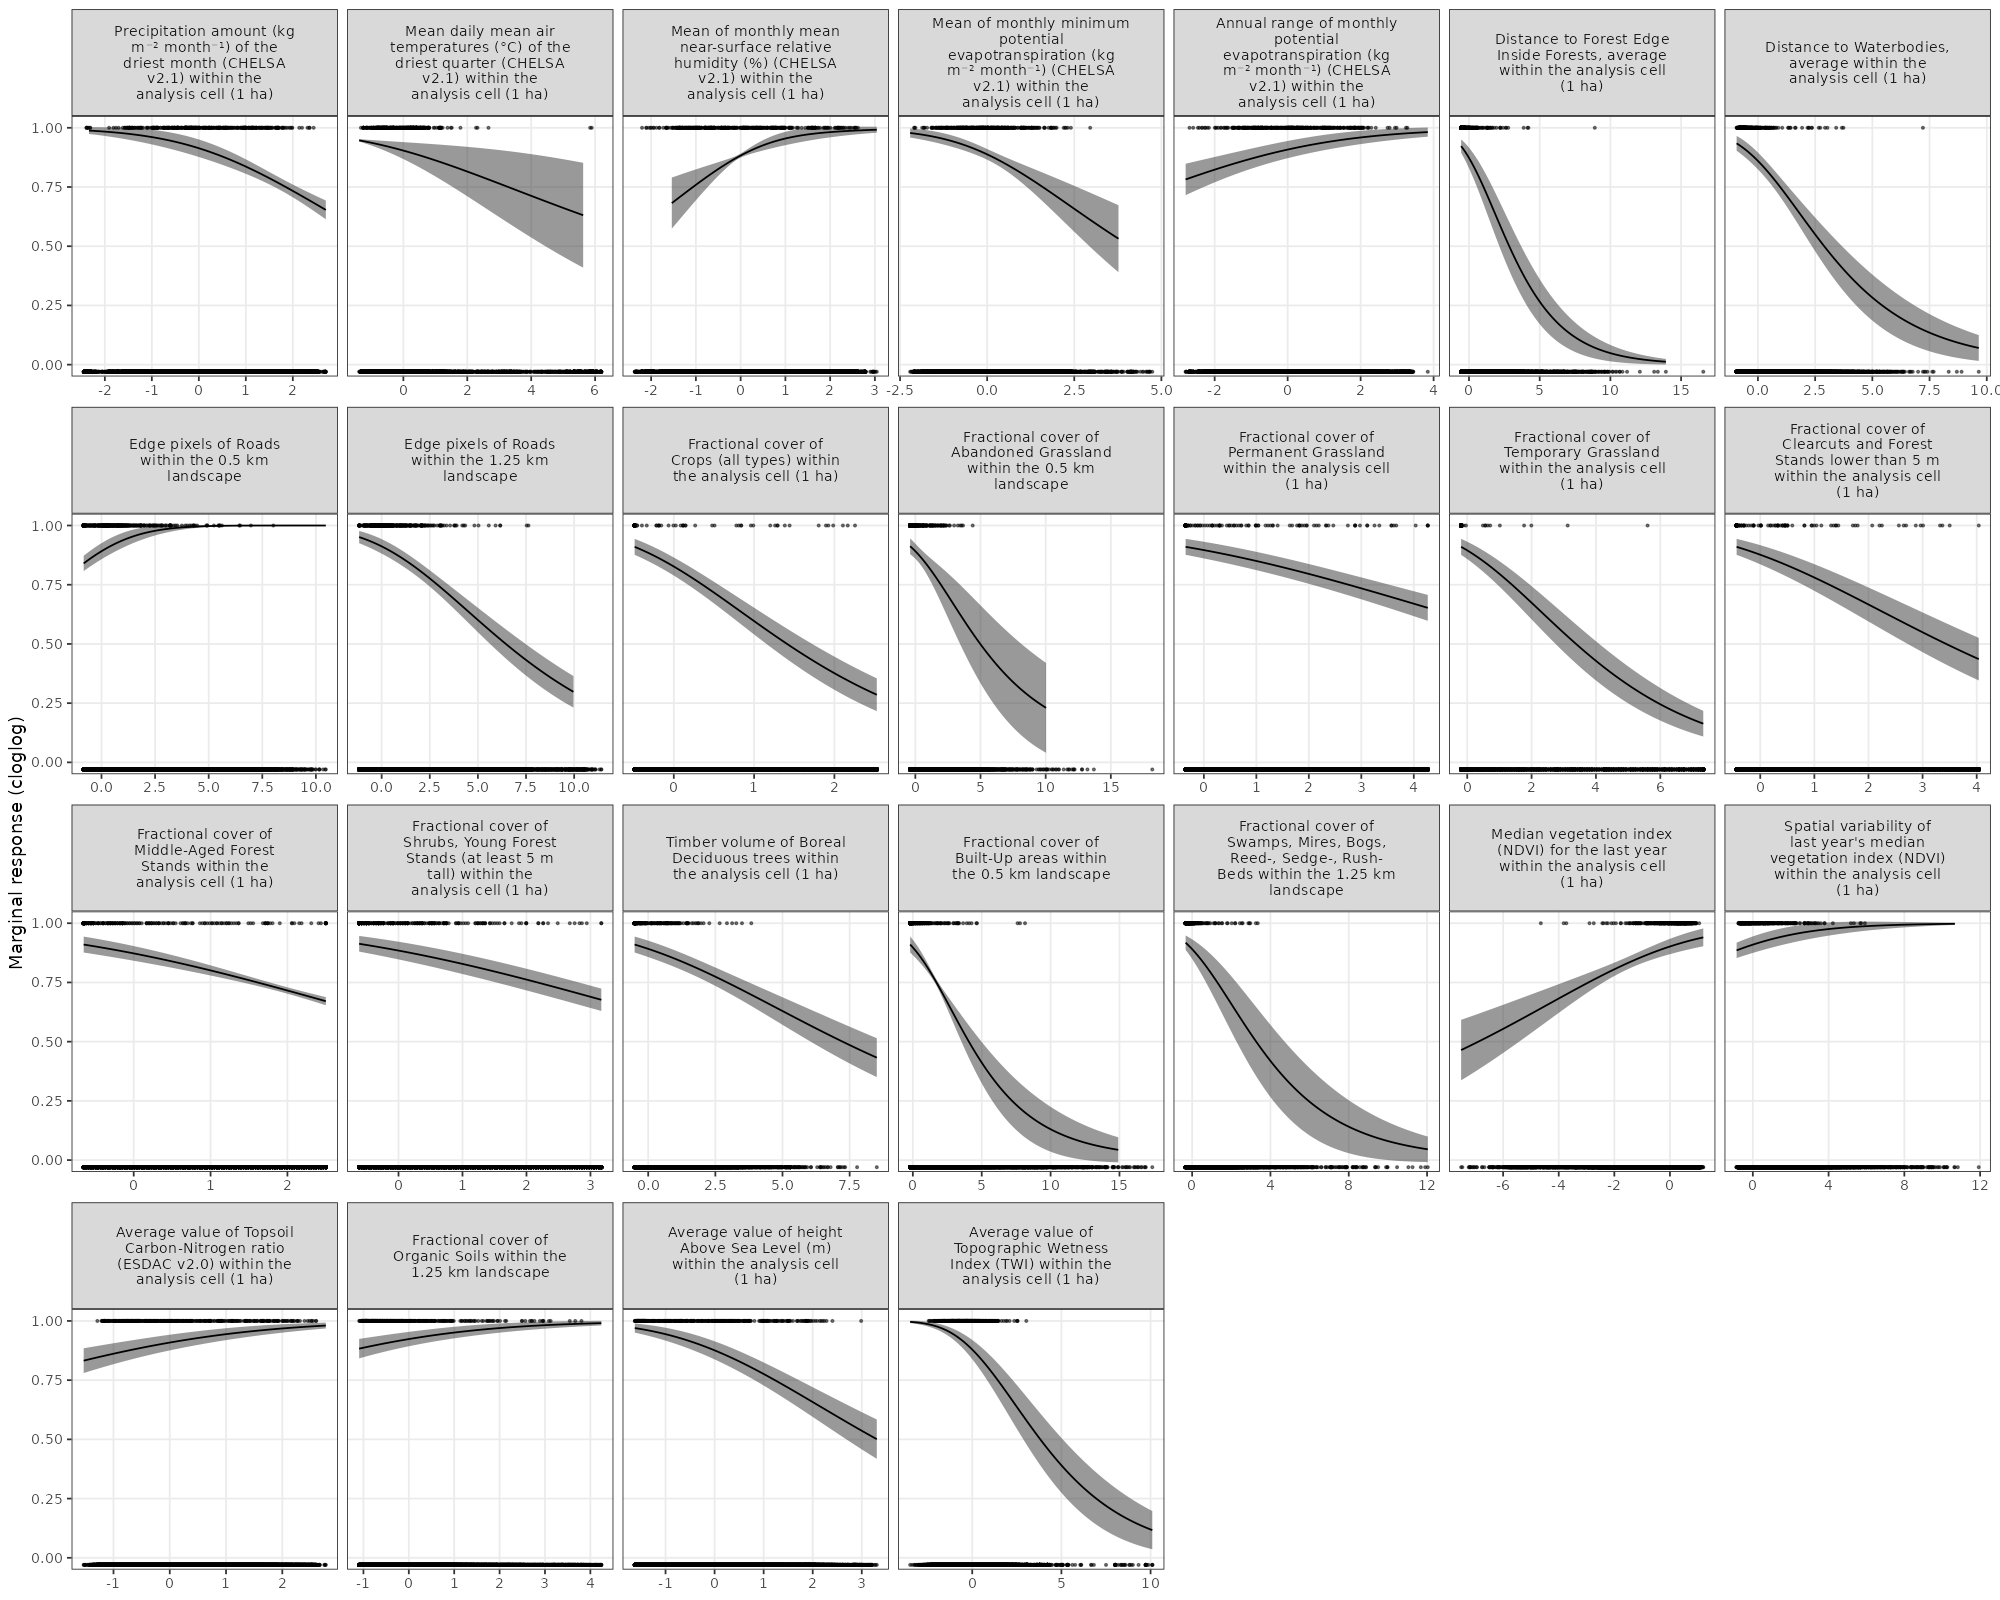
\includegraphics[width=1\linewidth,height=0.70\textheight,keepaspectratio]{results/BUFBUFv2bNM/PicMargResp_BUFBUF.png}

\par\small\textit{Marginalised for arithmetic mean response curves illustrating the effect of each ecogeographical variable on the habitat suitability when all the other variables have their arithmetic mean values. The y-axis shows the predicted habitat suitability (cloglog-transformed), while the x-axis shows the standardised (centred and scaled) value of the ecogeographical variable. Dots at a value of 1 on the y-axis illustrate presence locations in the environment (on the x-axis), while dots at a value of 0 illustrate background locations used in modelling.  **For a full resolution refer to repository: link or online document: link**}\normalsize
\end{center}

\section*{Habitat and conservation associations}\label{habitat-and-conservation-associations-9}
\addcontentsline{toc}{section}{Habitat and conservation associations}

\begin{center}
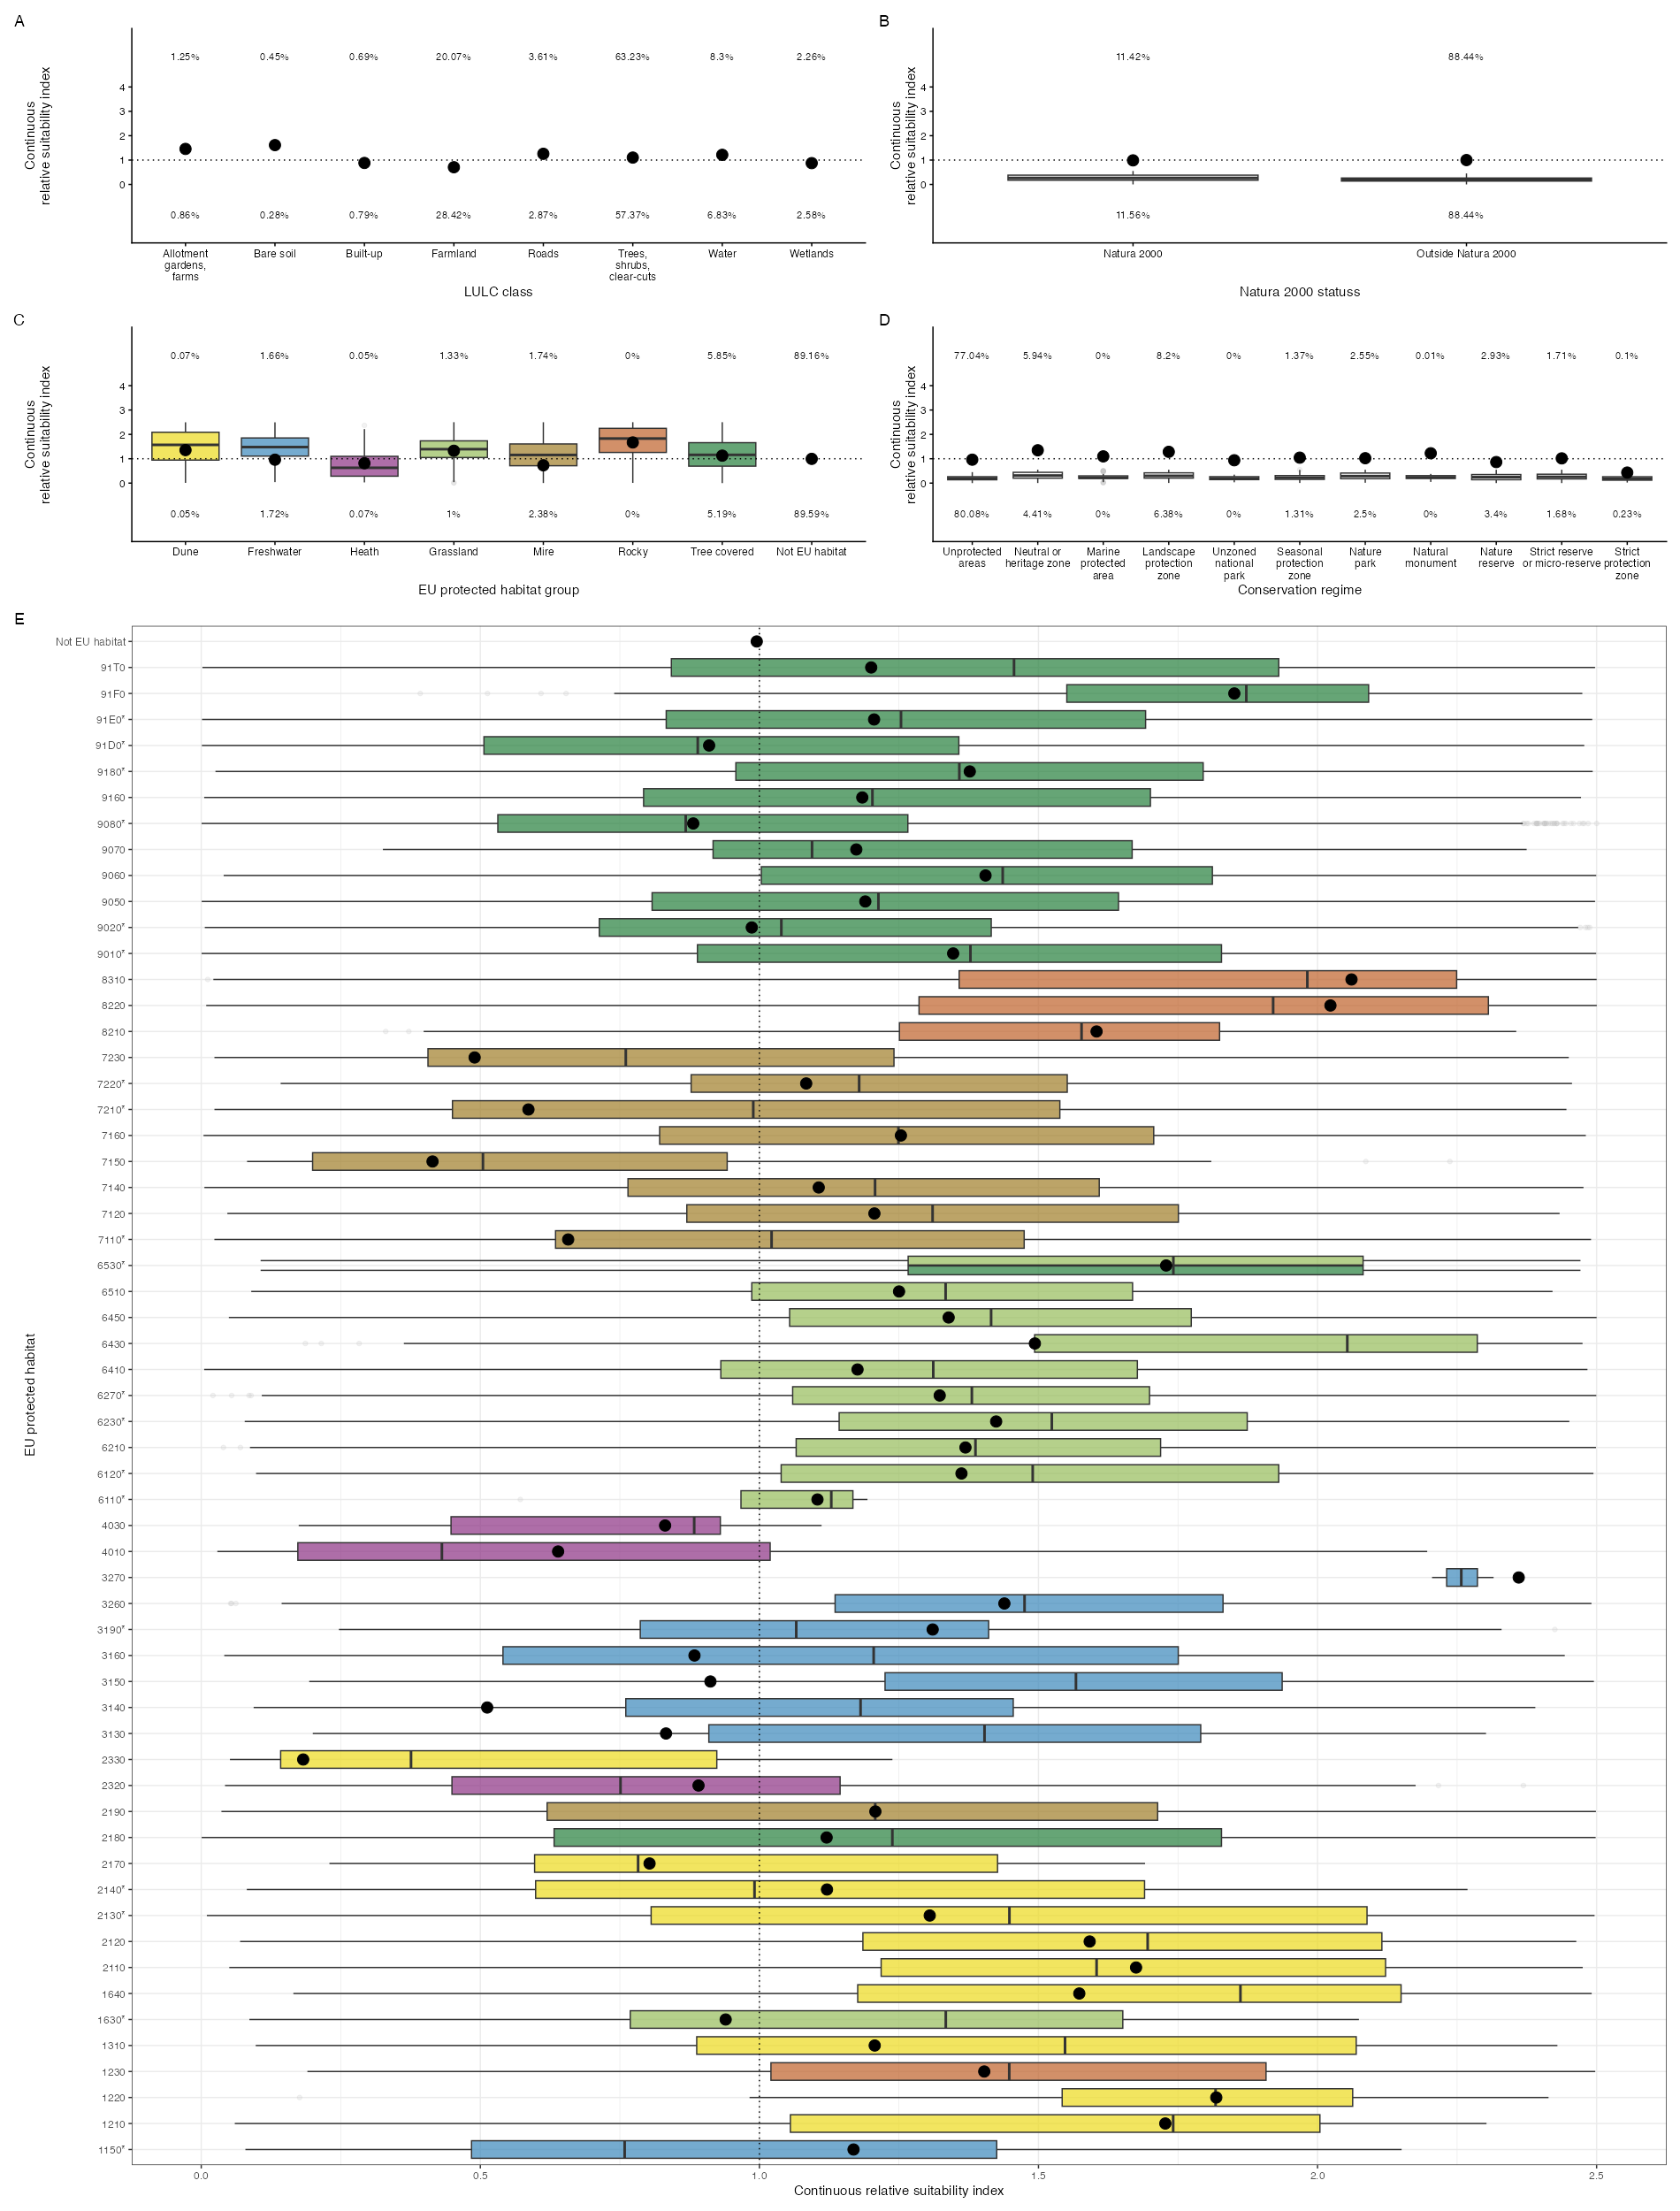
\includegraphics[width=1\linewidth,height=0.70\textheight,keepaspectratio]{results/BUFBUFv2bNM/PicAssoc_BUFBUF.png}

\par\small\textit{Associations between predicted suitability and: (A) land use land cover classes, (B) Natura 2000 status, (C) stratified EU protected habitat classes, (D) conservation regime, and (E) EU protected habitats. The y-axis show continuous relative suitability index (derivative of Manly's index of preference). Colours in (C) and (E) correspond to stratified EU protected habitat classes. For classifications composed of multiple individual polygons, polygon-level indices were additionally calculated to show within-category variation. The figures therefore combine category-level estimates (points) with the distributions of polygon-level values (boxplots, where applicable). Labels above and below the panels report, respectively, the percentage of total predicted suitability and the percentage of mapped area represented by each category. **For a full resolution refer to repository: link or online document: link**}\normalsize
\end{center}

\section*{Conservation prioritization}\label{conservation-prioritization-9}
\addcontentsline{toc}{section}{Conservation prioritization}

\begin{center}
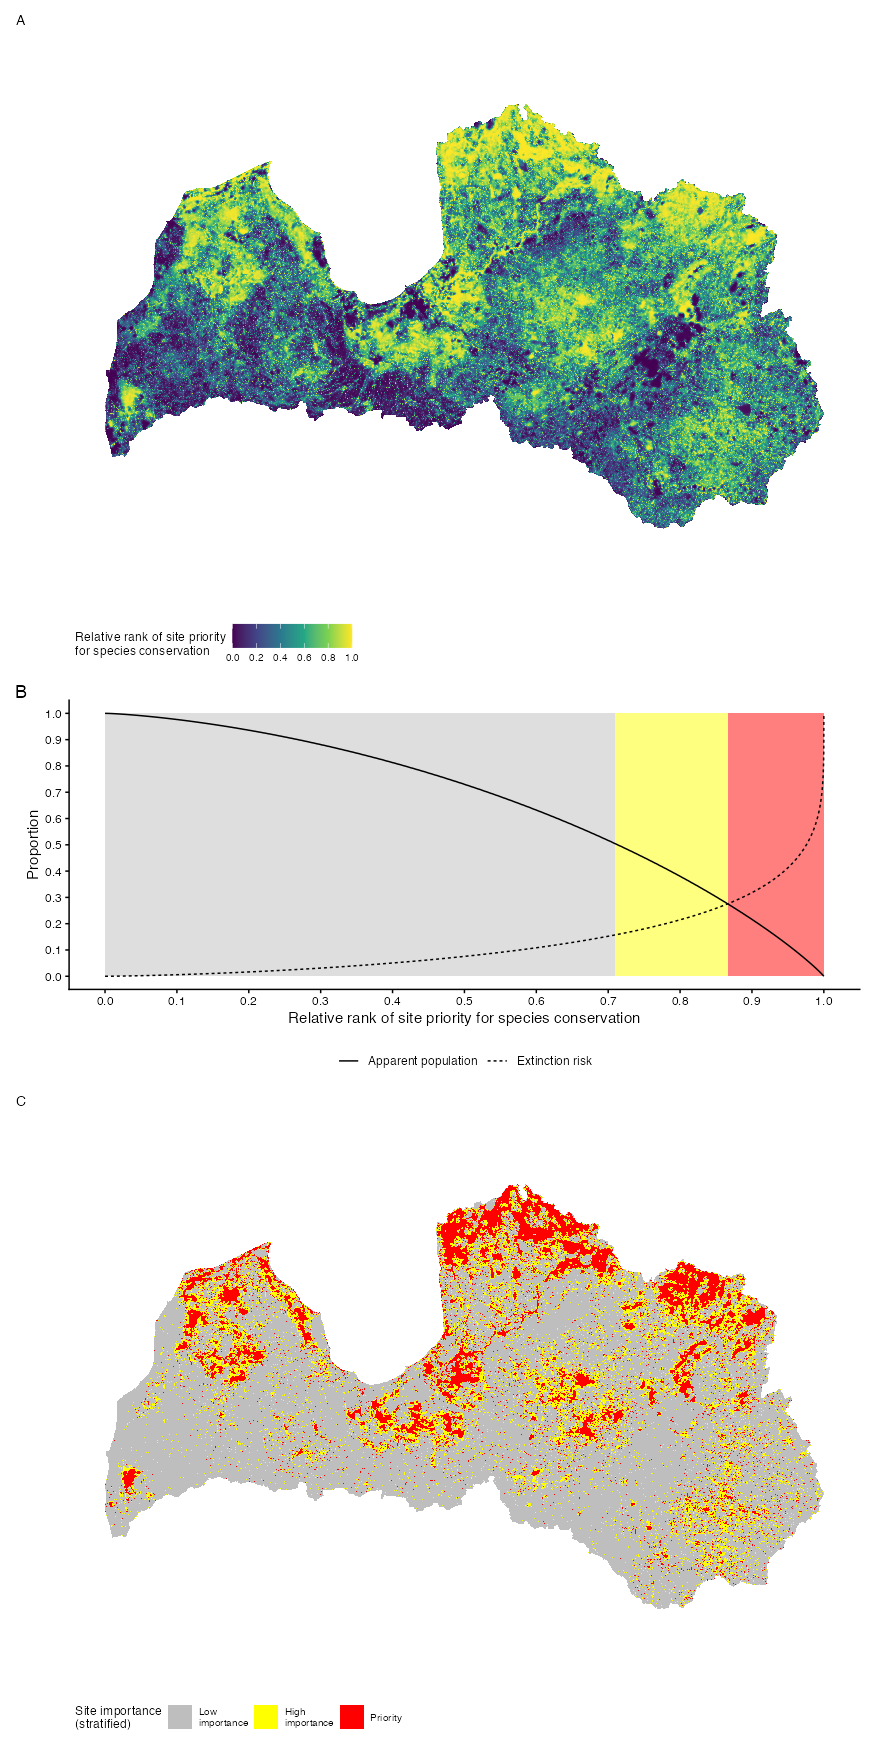
\includegraphics[width=0.85\linewidth,height=0.70\textheight,keepaspectratio]{results/BUFBUFv2bNM/PicPrior_BUFBUF.png}

\par\small\textit{Single-species conservation prioritization focusing on maximisation of core area protection (CAZMAX) while accounting for site connectivity: (A) relative site rank; (B) relationship between apparent-population and extinction-risk curves with a simplified classification which is spatially demonstrated in the bootom row; (C) spatial distribution of proposed classification of site prioritization results. **For a full resolution refer to repository: link or online document: link**}\normalsize
\end{center}

\chapter*{\texorpdfstring{\emph{Bufo bufo} terrestrial}{Bufo bufo terrestrial}}\label{bufbufterrestrial}
\addcontentsline{toc}{chapter}{\emph{Bufo bufo} terrestrial}

\section*{Summary}\label{summary-10}
\addcontentsline{toc}{section}{Summary}

\subsection*{Model description}\label{model-description-10}
\addcontentsline{toc}{subsection}{Model description}

Occurrence and background data were divided into model-training with four block spatial cross-validation data and an independent test set. Sampling-bias/background treatment: \textbf{Phenology Weighted Target Group}. Accumulated LULC change within the 1-ha analysis cell was not evaluated; accumulated LULC change within the home-range radius around the analysis cell was not evaluated.

The final data set contained \textbf{507} presence records: \textbf{380} for training with four spatial block cross-validation and \textbf{127} for independent testing. Training background contained \textbf{29981} locations, with \textbf{10019} additional independent-test background locations.

\subsection*{Expert assessment scores}\label{expert-assessment-scores-10}
\addcontentsline{toc}{subsection}{Expert assessment scores}

\begin{itemize}
\tightlist
\item
  \textbf{Marginal responses and variable importance score:} 2 (limited ecological interpretability)
\item
  \textbf{Map score:} 2 (limited agreement with known distribution)
\item
  \textbf{Applicability score:} 1 (very limited applicability)
\end{itemize}

\textbf{Šo sadaļu aizpildām manuāli no ekspertu aptaujām}

\subsection*{Statistical evaluation}\label{statistical-evaluation-10}
\addcontentsline{toc}{subsection}{Statistical evaluation}

The final model had a training TSS of \textbf{0.401}, with a training-derived cloglog threshold of \textbf{0.586}. Combined training AUC was \textbf{0.763} and combined test AUC was \textbf{0.71}.

\subsubsection*{Spatial cross-validation}\label{spatial-cross-validation-10}
\addcontentsline{toc}{subsubsection}{Spatial cross-validation}

\begin{itemize}
\tightlist
\item
  \textbf{AUC:} 0.692 ± 0.0615; null models: 0.5621 ± 0.0198; z = 6.5426, p \textless{} 0.001
\item
  \textbf{CBI:} 0.8778 ± 0.0093; null models: 0.3653 ± 0.1231; z = 4.1636, p \textless{} 0.001
\item
  \textbf{OR10:} 0.0921 ± 0.0481; null models: 0.0479 ± 0.0339; z = 1.3052, p = 0.904
\item
  \textbf{ORmin:} 0 ± 0; null models: 0.0029 ± 0.0111; z = -0.2641, p = 0.396
\end{itemize}

\subsubsection*{Independent testing}\label{independent-testing-10}
\addcontentsline{toc}{subsubsection}{Independent testing}

\begin{itemize}
\tightlist
\item
  \textbf{TSS:} 0.319; \textbf{sensitivity:} 0.622; \textbf{specificity:} 0.697
\item
  \textbf{AUC:} 0.685; null models: 0.5057 ± 0.0576; z = 3.1158, p = 0.001
\item
  \textbf{CBI:} 0.941; null models: 0.0121 ± 0.4417; z = 2.103, p = 0.018
\item
  \textbf{OR10:} 0.22; null models: 0.1256 ± 0.0568; z = 1.6712, p = 0.953
\item
  \textbf{ORmin:} 0.008; null models: 0.0031 ± 0.0056; z = 0.8602, p = 0.805
\end{itemize}

\subsection*{Conservation prioritisation summary}\label{conservation-prioritisation-summary-10}
\addcontentsline{toc}{subsection}{Conservation prioritisation summary}

The primary priority area covers \textbf{15.1\%} of Latvia and contains \textbf{27.6\%} of the summed habitat suitability (apparent population proxy).

The broader high importance area covers \textbf{28.4\%} of Latvia and contains \textbf{46.5\%} of the summed habitat suitability.

For comparison, the area classified as suitable using the maximum training sensitivity plus specificity habitat-suitability threshold contains \textbf{46.5\%} of the summed continuous habitat suitability.

\subsection*{Version evolution}\label{version-evolution-10}
\addcontentsline{toc}{subsection}{Version evolution}

\textbf{Šo sadaļu aizpildām manuāli, izmntojot sagatavotās shēmas. Jāvienojas par to noformējumu}

\section*{Habitat suitability}\label{habitat-suitability-10}
\addcontentsline{toc}{section}{Habitat suitability}

\begin{center}
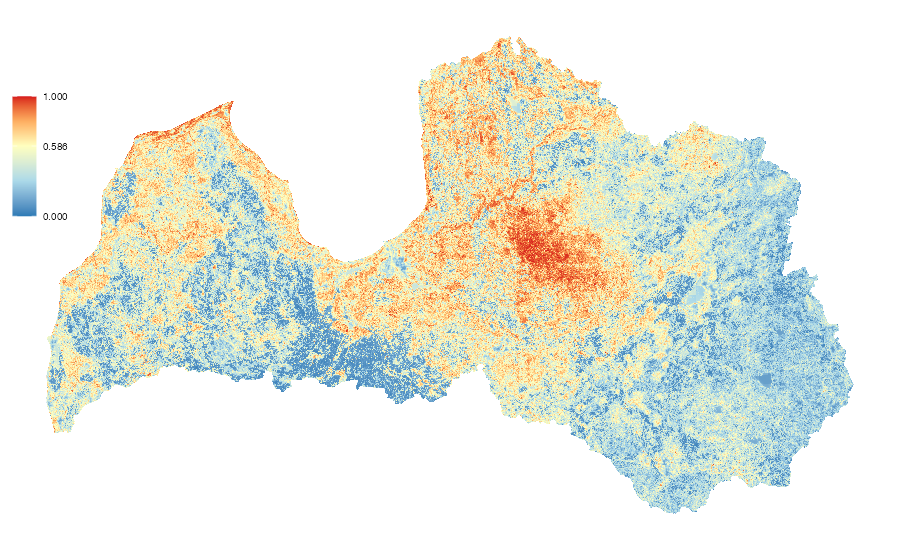
\includegraphics[width=1\linewidth,height=0.70\textheight,keepaspectratio]{results/BUFBUFterrestrialv2b1celi/PicHSmap_BUFBUFterrestrial.png}

\par\small\textit{Predicted continuous habitat suitability across Latvia. The warmer the colour the higher is the predicted habitat suitability. Value in the middle of the legend correspond to the maximum training sensitivity plus specificity threshold. **For a full resolution refer to repository: link or online document: link**}\normalsize
\end{center}

\section*{Model thresholds}\label{model-thresholds-10}
\addcontentsline{toc}{section}{Model thresholds}

Threshold values and associated omission rates

\begin{center}
\resizebox{\linewidth}{!}{%

\begin{tabular}{lrrrrr}
\toprule
Threshold & Cloglog value & Fractional predicted area & Training omission rate & Test omission rate & P-values\\
\midrule
Minimum training presence & 0.1416890 & 0.9330270 & 0.0000000 & 0.0000978 & 0\\
Equal training sensitivity and specificity & 0.6037913 & 0.3052792 & 0.3052632 & 0.0052817 & 0\\
Maximum training sensitivity plus specificity & 0.5861025 & 0.3334766 & 0.2684211 & 0.0046948 & 0\\
Equal test sensitivity and specificity & 0.5634530 & 0.3666325 & 0.2526316 & 0.0041080 & 0\\
Maximum test sensitivity plus specificity & 0.5524573 & 0.3831609 & 0.2421053 & 0.0037167 & 0\\
\bottomrule
\end{tabular}
}
\end{center}

\section*{Variable importance}\label{variable-importance-10}
\addcontentsline{toc}{section}{Variable importance}

\begin{center}
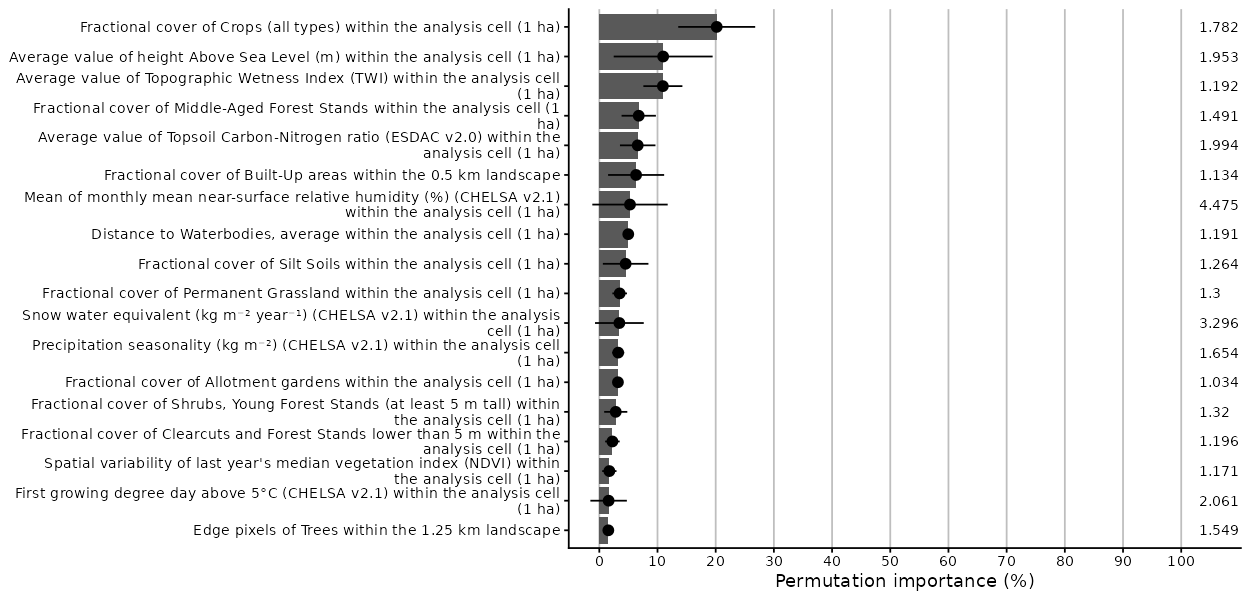
\includegraphics[width=1\linewidth,height=0.70\textheight,keepaspectratio]{results/BUFBUFterrestrialv2b1celi/PicVarImpVIFs_BUFBUFterrestrial.png}

\par\small\textit{Permutation-importance (mean and standard deviation from 99 permutations, on the x-axis) of the ecogeographical variables (first y-axis, left side), and their variance inflation factor values (second y-axis, right side). **For a full resolution refer to repository: link or online document: link**}\normalsize
\end{center}

\section*{Marginal responses}\label{marginal-responses-10}
\addcontentsline{toc}{section}{Marginal responses}

\begin{center}
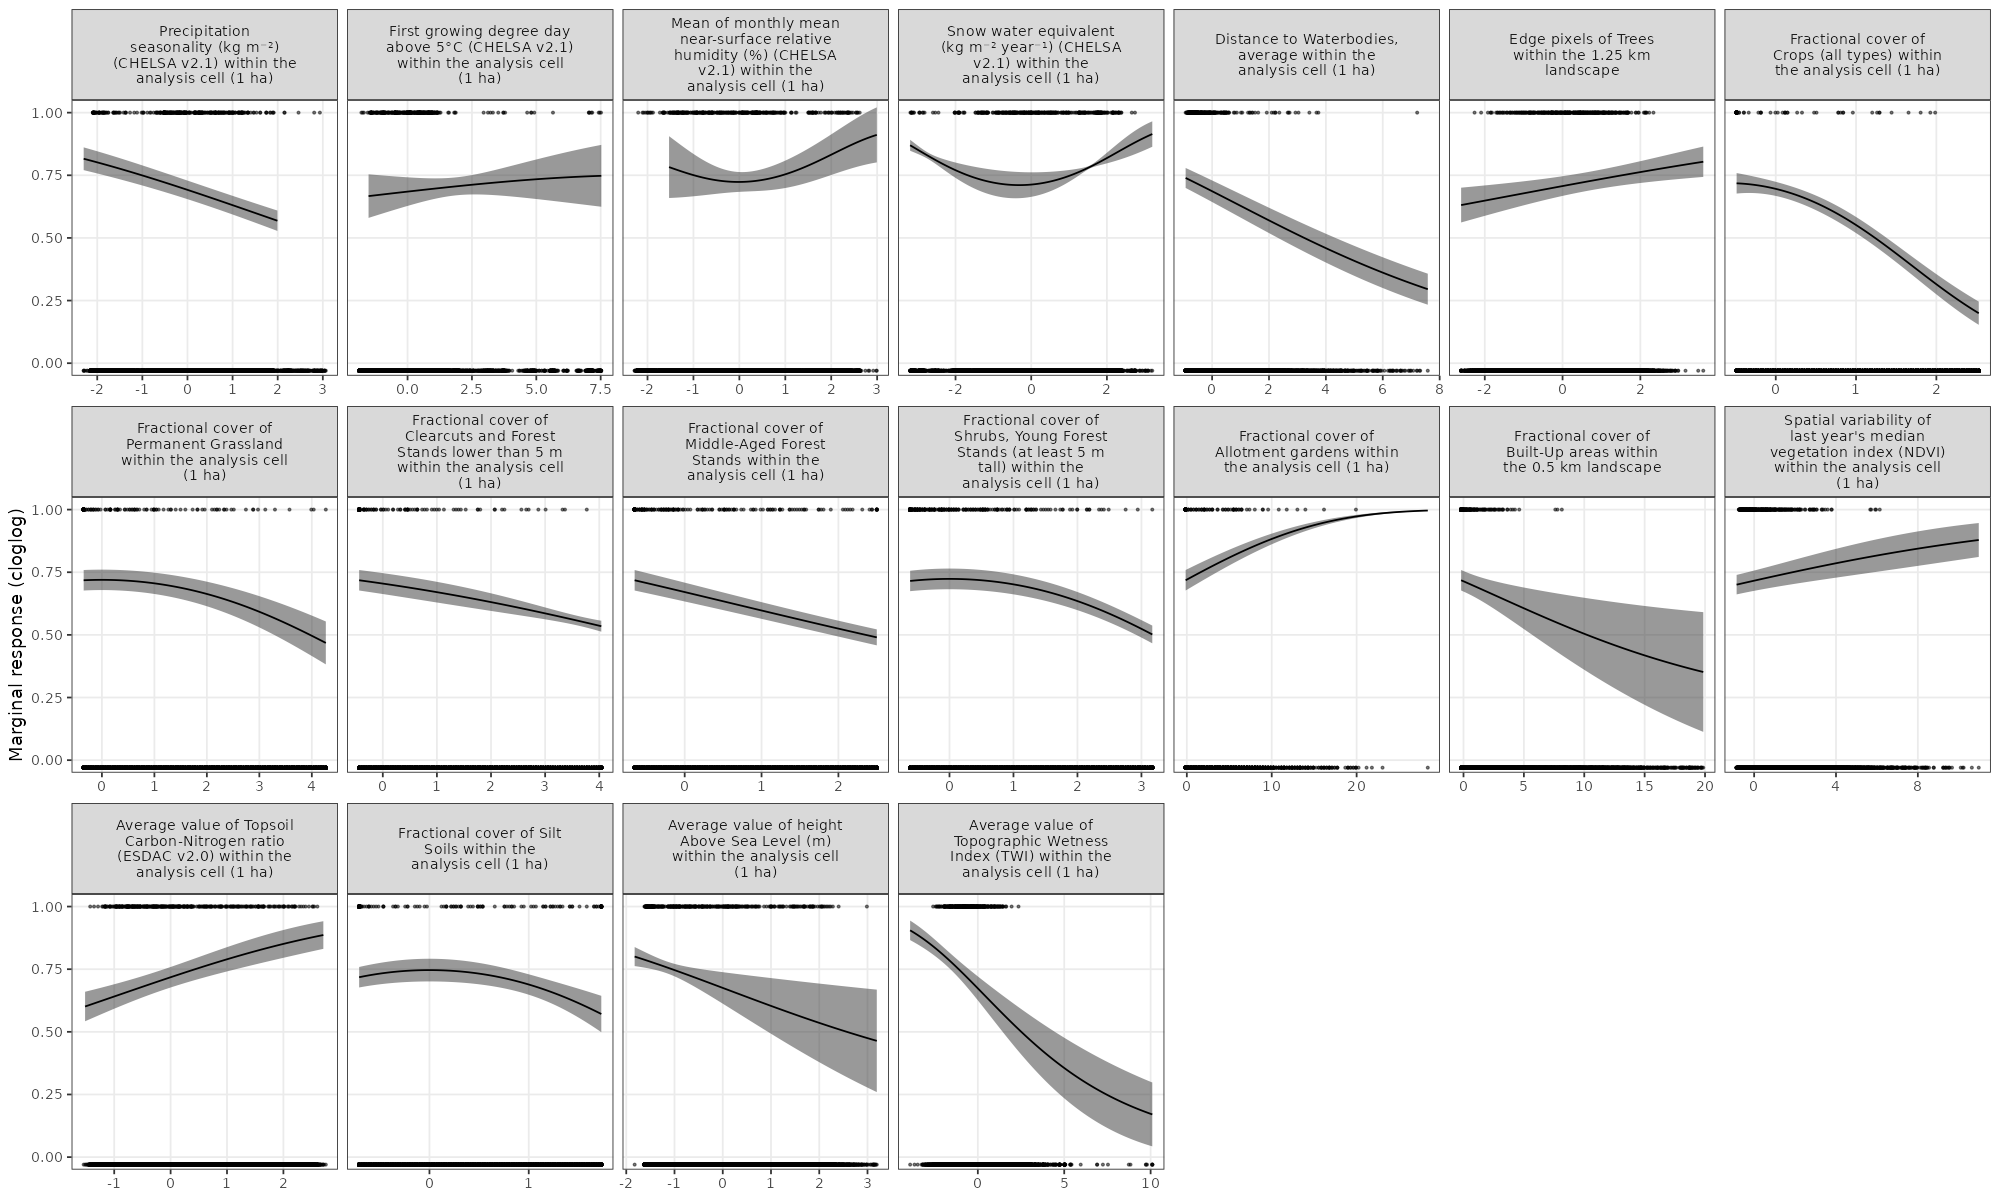
\includegraphics[width=1\linewidth,height=0.70\textheight,keepaspectratio]{results/BUFBUFterrestrialv2b1celi/PicMargResp_BUFBUFterrestrial.png}

\par\small\textit{Marginalised for arithmetic mean response curves illustrating the effect of each ecogeographical variable on the habitat suitability when all the other variables have their arithmetic mean values. The y-axis shows the predicted habitat suitability (cloglog-transformed), while the x-axis shows the standardised (centred and scaled) value of the ecogeographical variable. Dots at a value of 1 on the y-axis illustrate presence locations in the environment (on the x-axis), while dots at a value of 0 illustrate background locations used in modelling.  **For a full resolution refer to repository: link or online document: link**}\normalsize
\end{center}

\section*{Habitat and conservation associations}\label{habitat-and-conservation-associations-10}
\addcontentsline{toc}{section}{Habitat and conservation associations}

\begin{center}
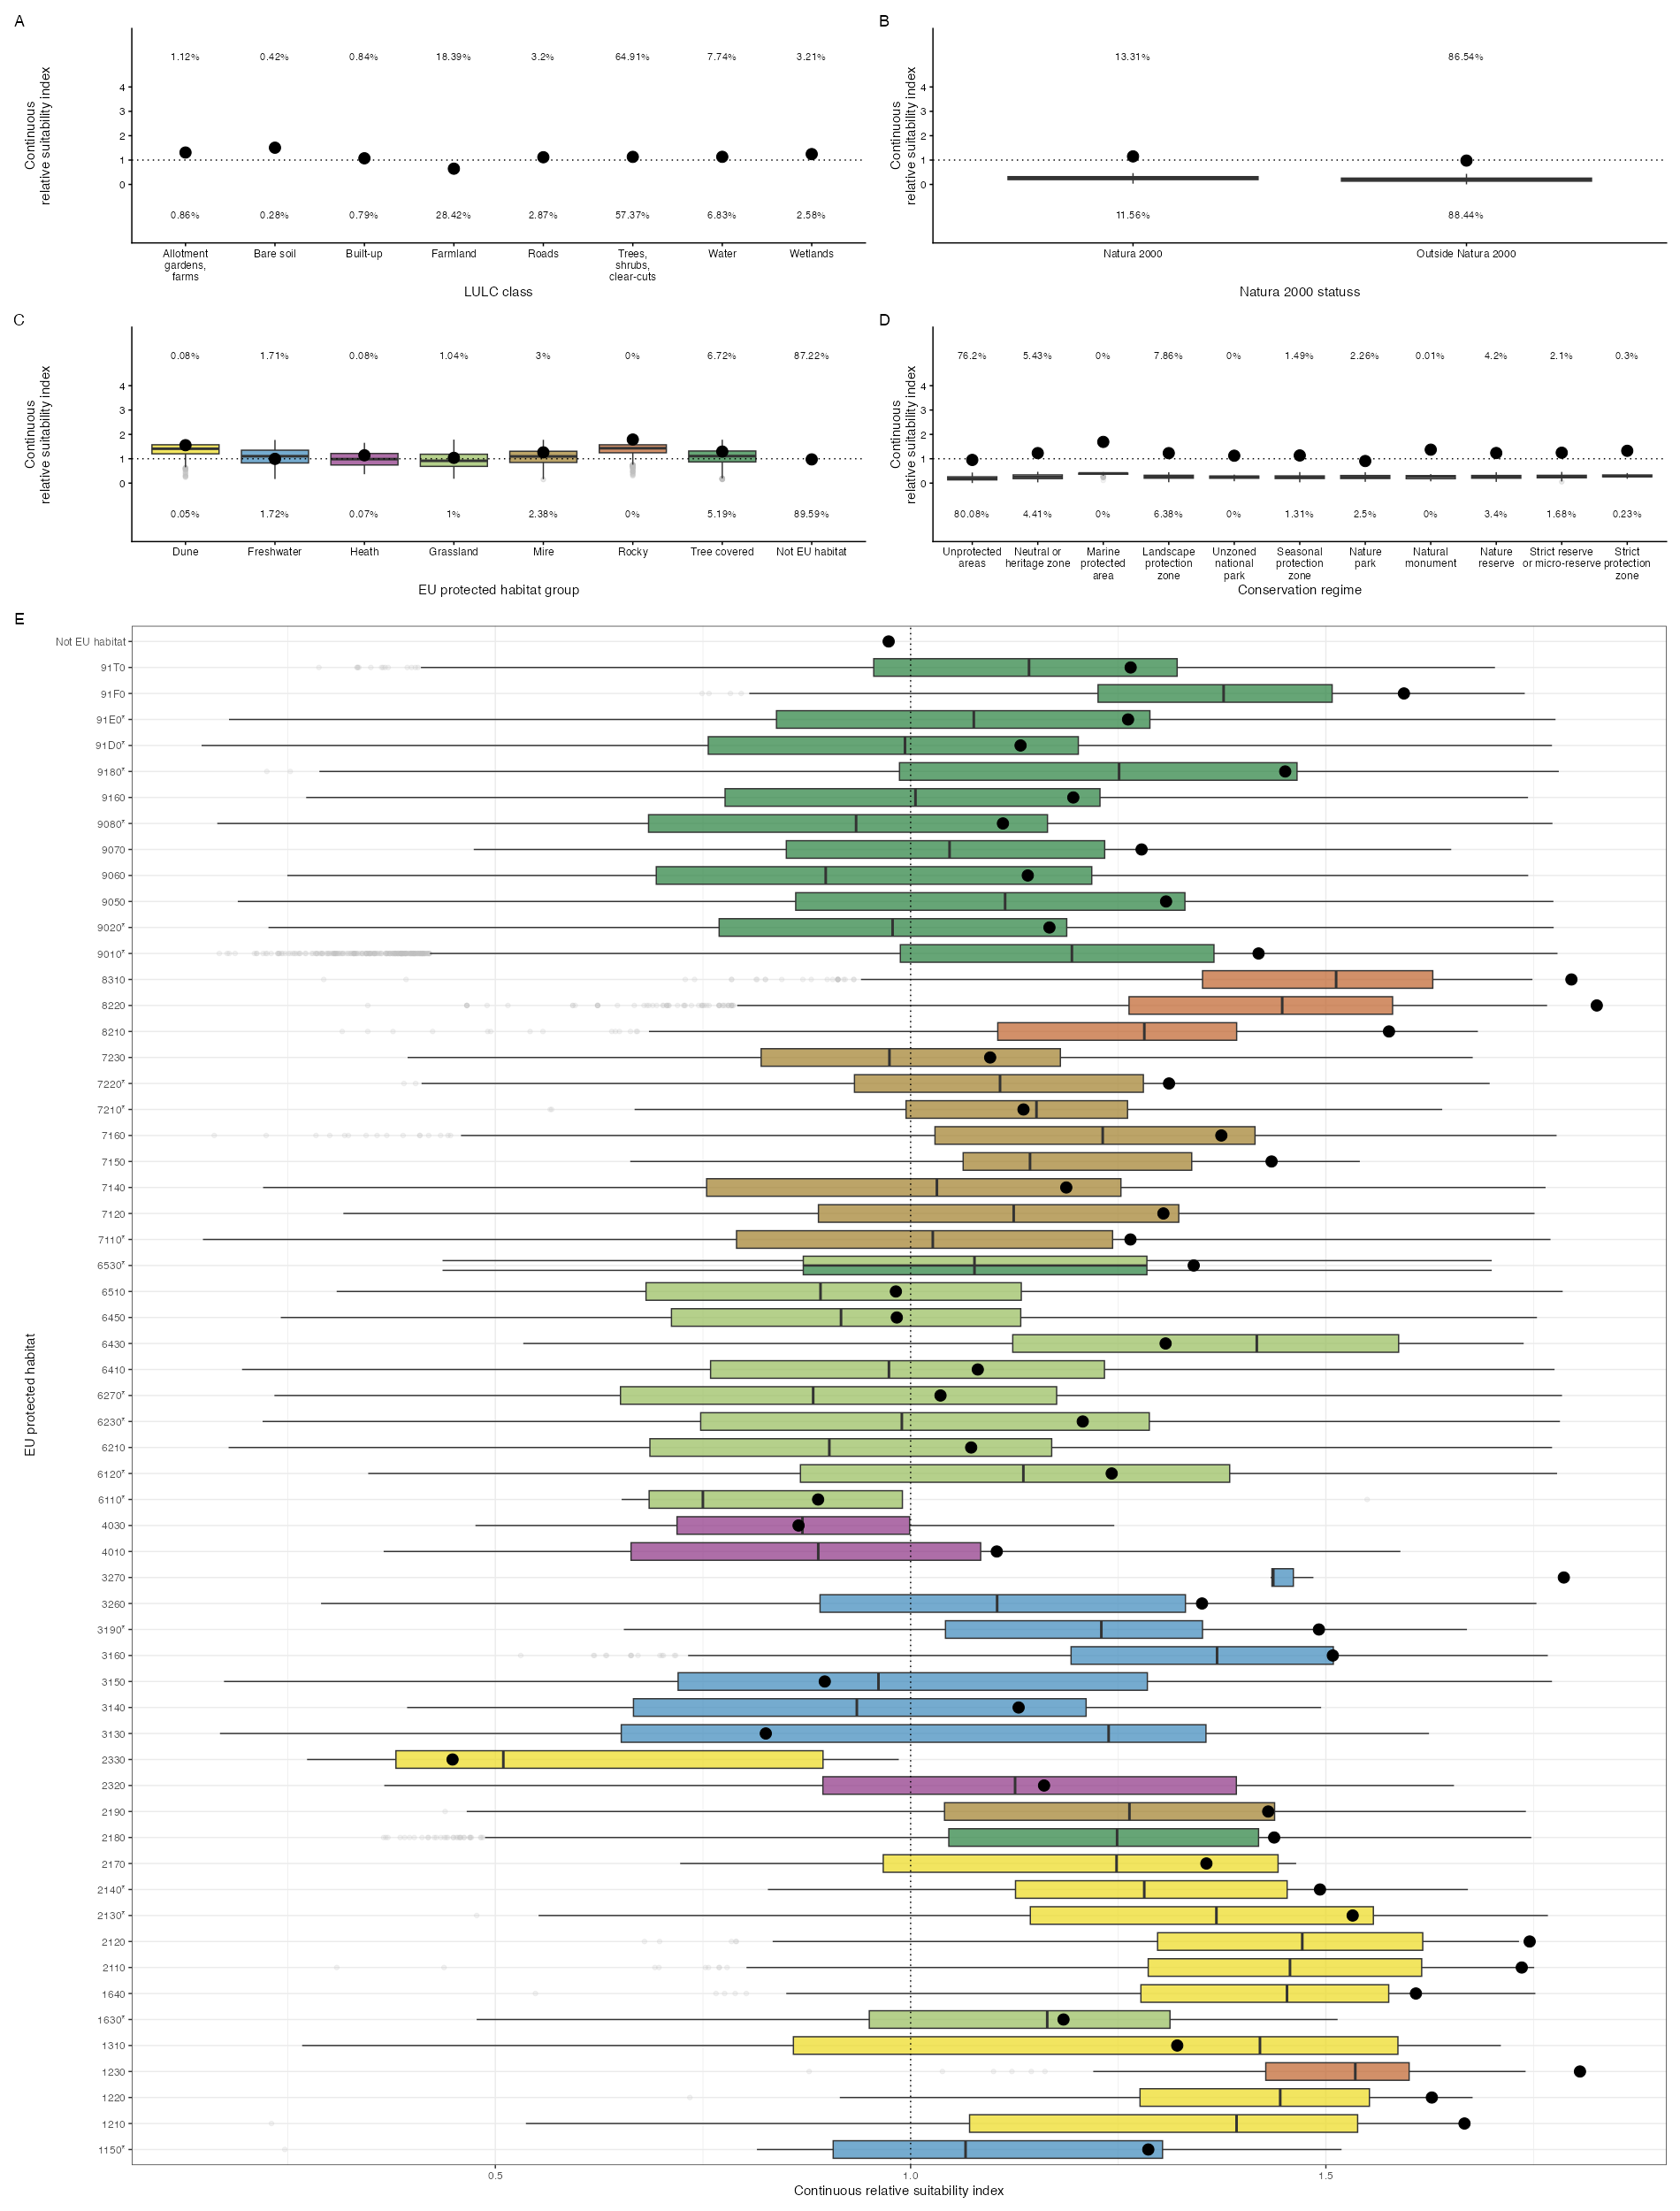
\includegraphics[width=1\linewidth,height=0.70\textheight,keepaspectratio]{results/BUFBUFterrestrialv2b1celi/PicAssoc_BUFBUFterrestrial.png}

\par\small\textit{Associations between predicted suitability and: (A) land use land cover classes, (B) Natura 2000 status, (C) stratified EU protected habitat classes, (D) conservation regime, and (E) EU protected habitats. The y-axis show continuous relative suitability index (derivative of Manly's index of preference). Colours in (C) and (E) correspond to stratified EU protected habitat classes. For classifications composed of multiple individual polygons, polygon-level indices were additionally calculated to show within-category variation. The figures therefore combine category-level estimates (points) with the distributions of polygon-level values (boxplots, where applicable). Labels above and below the panels report, respectively, the percentage of total predicted suitability and the percentage of mapped area represented by each category. **For a full resolution refer to repository: link or online document: link**}\normalsize
\end{center}

\section*{Conservation prioritization}\label{conservation-prioritization-10}
\addcontentsline{toc}{section}{Conservation prioritization}

\begin{center}
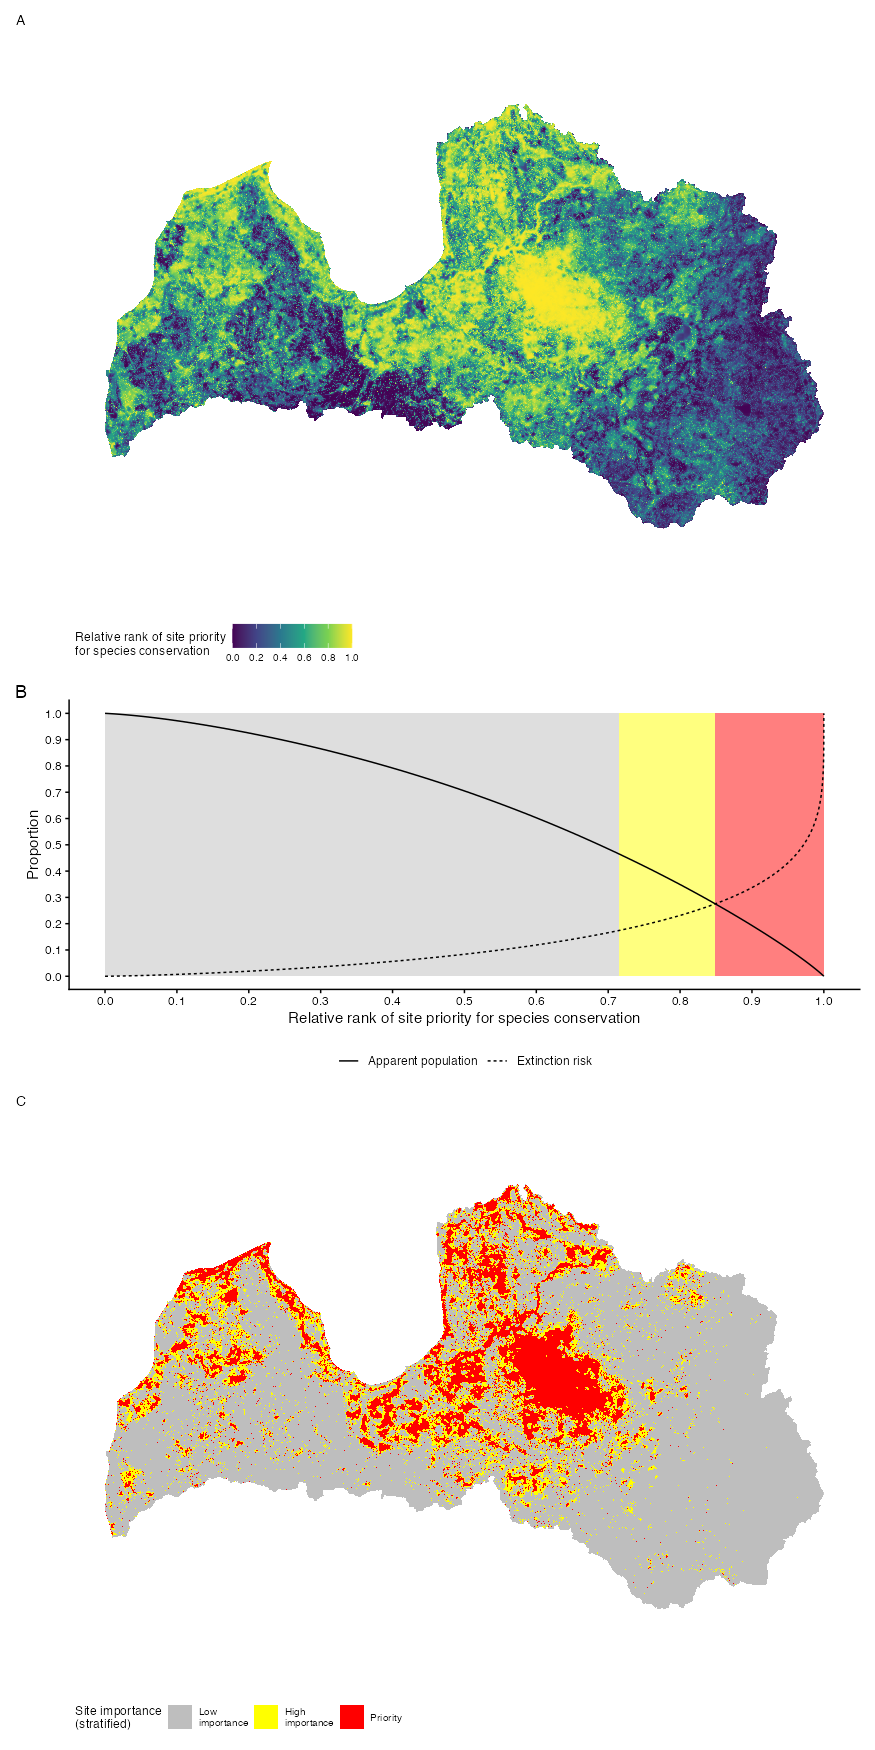
\includegraphics[width=0.85\linewidth,height=0.70\textheight,keepaspectratio]{results/BUFBUFterrestrialv2b1celi/PicPrior_BUFBUFterrestrial.png}

\par\small\textit{Single-species conservation prioritization focusing on maximisation of core area protection (CAZMAX) while accounting for site connectivity: (A) relative site rank; (B) relationship between apparent-population and extinction-risk curves with a simplified classification which is spatially demonstrated in the bootom row; (C) spatial distribution of proposed classification of site prioritization results. **For a full resolution refer to repository: link or online document: link**}\normalsize
\end{center}

\chapter*{\texorpdfstring{\emph{Bufo bufo} monitoring}{Bufo bufo monitoring}}\label{bufbufmonitoring}
\addcontentsline{toc}{chapter}{\emph{Bufo bufo} monitoring}

\section*{Summary}\label{summary-11}
\addcontentsline{toc}{section}{Summary}

\subsection*{Model description}\label{model-description-11}
\addcontentsline{toc}{subsection}{Model description}

Occurrence and background data were divided into model-training with four block spatial cross-validation data and an independent test set. Sampling-bias/background treatment: \textbf{Phenology Weighted Target Group}. Accumulated LULC change within the 1-ha analysis cell was not evaluated; accumulated LULC change within the home-range radius around the analysis cell was not evaluated.

The final data set contained \textbf{947} presence records: \textbf{710} for training with four spatial block cross-validation and \textbf{237} for independent testing. Training background contained \textbf{29990} locations, with \textbf{10010} additional independent-test background locations.

\subsection*{Expert assessment scores}\label{expert-assessment-scores-11}
\addcontentsline{toc}{subsection}{Expert assessment scores}

\begin{itemize}
\tightlist
\item
  \textbf{Marginal responses and variable importance score:} 4 (good ecological interpretability)
\item
  \textbf{Map score:} 2 (limited agreement with known distribution)
\item
  \textbf{Applicability score:} 2 (limited applicability)
\end{itemize}

\textbf{Šo sadaļu aizpildām manuāli no ekspertu aptaujām}

\subsection*{Statistical evaluation}\label{statistical-evaluation-11}
\addcontentsline{toc}{subsection}{Statistical evaluation}

The final model had a training TSS of \textbf{0.401}, with a training-derived cloglog threshold of \textbf{0.527}. Combined training AUC was \textbf{0.845} and combined test AUC was \textbf{0.849}.

\subsubsection*{Spatial cross-validation}\label{spatial-cross-validation-11}
\addcontentsline{toc}{subsubsection}{Spatial cross-validation}

\begin{itemize}
\tightlist
\item
  \textbf{AUC:} 0.8481 ± 0.0229; null models: 0.537 ± 0.0312; z = 9.9626, p \textless{} 0.001
\item
  \textbf{CBI:} 0.9752 ± 0.0131; null models: 0.2565 ± 0.1992; z = 3.6084, p \textless{} 0.001
\item
  \textbf{OR10:} 0.1156 ± 0.0548; null models: 0.0766 ± 0.0416; z = 0.9373, p = 0.826
\item
  \textbf{ORmin:} 0.0014 ± 0.0028; null models: 0.0016 ± 0.0049; z = -0.0414, p = 0.483
\end{itemize}

\subsubsection*{Independent testing}\label{independent-testing-11}
\addcontentsline{toc}{subsubsection}{Independent testing}

\begin{itemize}
\tightlist
\item
  \textbf{TSS:} 0.547; \textbf{sensitivity:} 0.793; \textbf{specificity:} 0.754
\item
  \textbf{AUC:} 0.84; null models: 0.5382 ± 0.099; z = 3.0479, p = 0.001
\item
  \textbf{CBI:} 0.983; null models: 0.229 ± 0.6043; z = 1.2477, p = 0.106
\item
  \textbf{OR10:} 0.11; null models: 0.0602 ± 0.0523; z = 0.9476, p = 0.828
\item
  \textbf{ORmin:} 0; null models: 4e-04 ± 0.0017; z = -0.2413, p = 0.405
\end{itemize}

\subsection*{Conservation prioritisation summary}\label{conservation-prioritisation-summary-11}
\addcontentsline{toc}{subsection}{Conservation prioritisation summary}

The primary priority area covers \textbf{11.9\%} of Latvia and contains \textbf{27.6\%} of the summed habitat suitability (apparent population proxy).

The broader high importance area covers \textbf{22.9\%} of Latvia and contains \textbf{46.2\%} of the summed habitat suitability.

For comparison, the area classified as suitable using the maximum training sensitivity plus specificity habitat-suitability threshold contains \textbf{46.2\%} of the summed continuous habitat suitability.

\subsection*{Version evolution}\label{version-evolution-11}
\addcontentsline{toc}{subsection}{Version evolution}

\textbf{Šo sadaļu aizpildām manuāli, izmntojot sagatavotās shēmas. Jāvienojas par to noformējumu}

\section*{Habitat suitability}\label{habitat-suitability-11}
\addcontentsline{toc}{section}{Habitat suitability}

\begin{center}
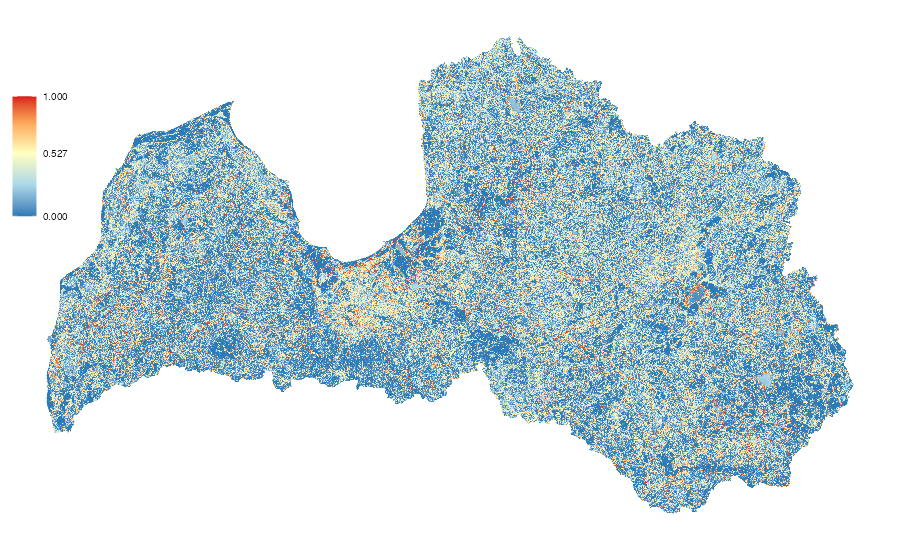
\includegraphics[width=1\linewidth,height=0.70\textheight,keepaspectratio]{results/BUFBUFmonitoringv2b5celi/PicHSmap_BUFBUFmonitoring.png}

\par\small\textit{Predicted continuous habitat suitability across Latvia. The warmer the colour the higher is the predicted habitat suitability. Value in the middle of the legend correspond to the maximum training sensitivity plus specificity threshold. **For a full resolution refer to repository: link or online document: link**}\normalsize
\end{center}

\section*{Model thresholds}\label{model-thresholds-11}
\addcontentsline{toc}{section}{Model thresholds}

Threshold values and associated omission rates

\begin{center}
\resizebox{\linewidth}{!}{%

\begin{tabular}{lrrrrr}
\toprule
Threshold & Cloglog value & Fractional predicted area & Training omission rate & Test omission rate & P-values\\
\midrule
Minimum training presence & 0.0000138 & 0.9923280 & 0.0000000 & 0.0000000 & 0\\
Equal training sensitivity and specificity & 0.5656726 & 0.2288443 & 0.2295775 & 0.0060670 & 0\\
Maximum training sensitivity plus specificity & 0.5272606 & 0.2640764 & 0.1732394 & 0.0047188 & 0\\
Equal test sensitivity and specificity & 0.5427962 & 0.2498189 & 0.2028169 & 0.0052966 & 0\\
Maximum test sensitivity plus specificity & 0.4847596 & 0.3015147 & 0.1521127 & 0.0028891 & 0\\
\bottomrule
\end{tabular}
}
\end{center}

\section*{Variable importance}\label{variable-importance-11}
\addcontentsline{toc}{section}{Variable importance}

\begin{center}
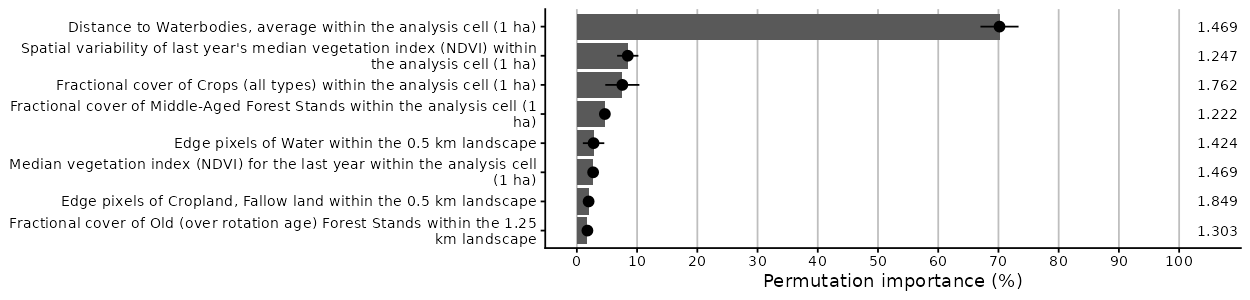
\includegraphics[width=1\linewidth,height=0.70\textheight,keepaspectratio]{results/BUFBUFmonitoringv2b5celi/PicVarImpVIFs_BUFBUFmonitoring.png}

\par\small\textit{Permutation-importance (mean and standard deviation from 99 permutations, on the x-axis) of the ecogeographical variables (first y-axis, left side), and their variance inflation factor values (second y-axis, right side). **For a full resolution refer to repository: link or online document: link**}\normalsize
\end{center}

\section*{Marginal responses}\label{marginal-responses-11}
\addcontentsline{toc}{section}{Marginal responses}

\begin{center}
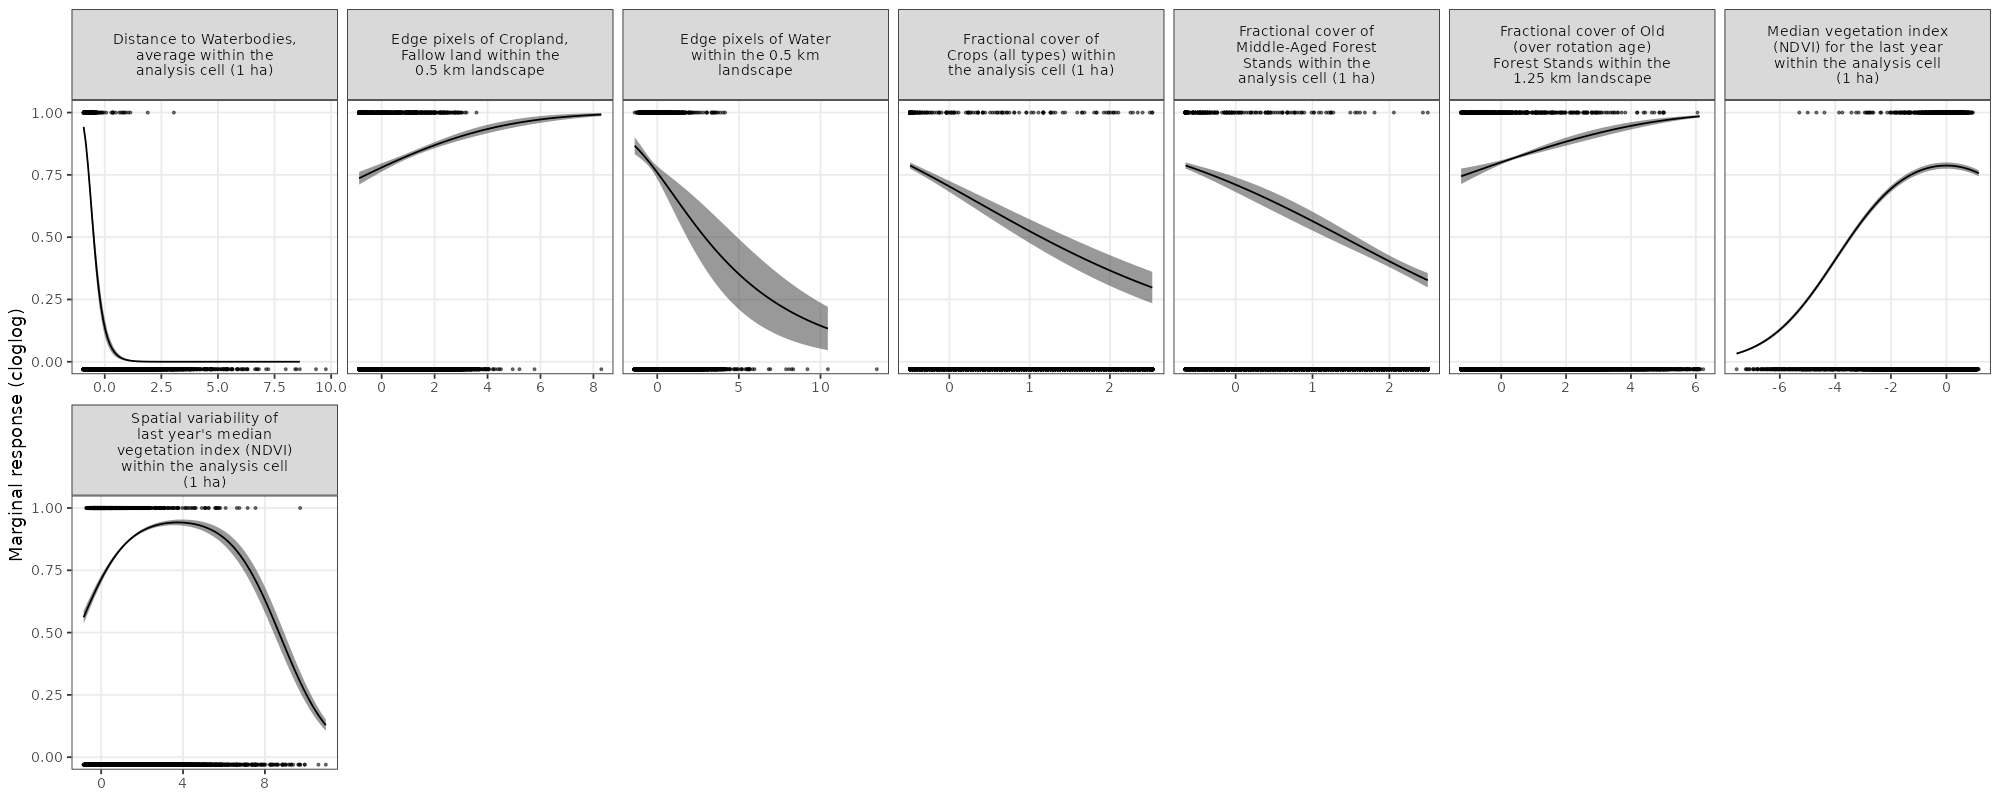
\includegraphics[width=1\linewidth,height=0.70\textheight,keepaspectratio]{results/BUFBUFmonitoringv2b5celi/PicMargResp_BUFBUFmonitoring.png}

\par\small\textit{Marginalised for arithmetic mean response curves illustrating the effect of each ecogeographical variable on the habitat suitability when all the other variables have their arithmetic mean values. The y-axis shows the predicted habitat suitability (cloglog-transformed), while the x-axis shows the standardised (centred and scaled) value of the ecogeographical variable. Dots at a value of 1 on the y-axis illustrate presence locations in the environment (on the x-axis), while dots at a value of 0 illustrate background locations used in modelling.  **For a full resolution refer to repository: link or online document: link**}\normalsize
\end{center}

\section*{Habitat and conservation associations}\label{habitat-and-conservation-associations-11}
\addcontentsline{toc}{section}{Habitat and conservation associations}

\begin{center}
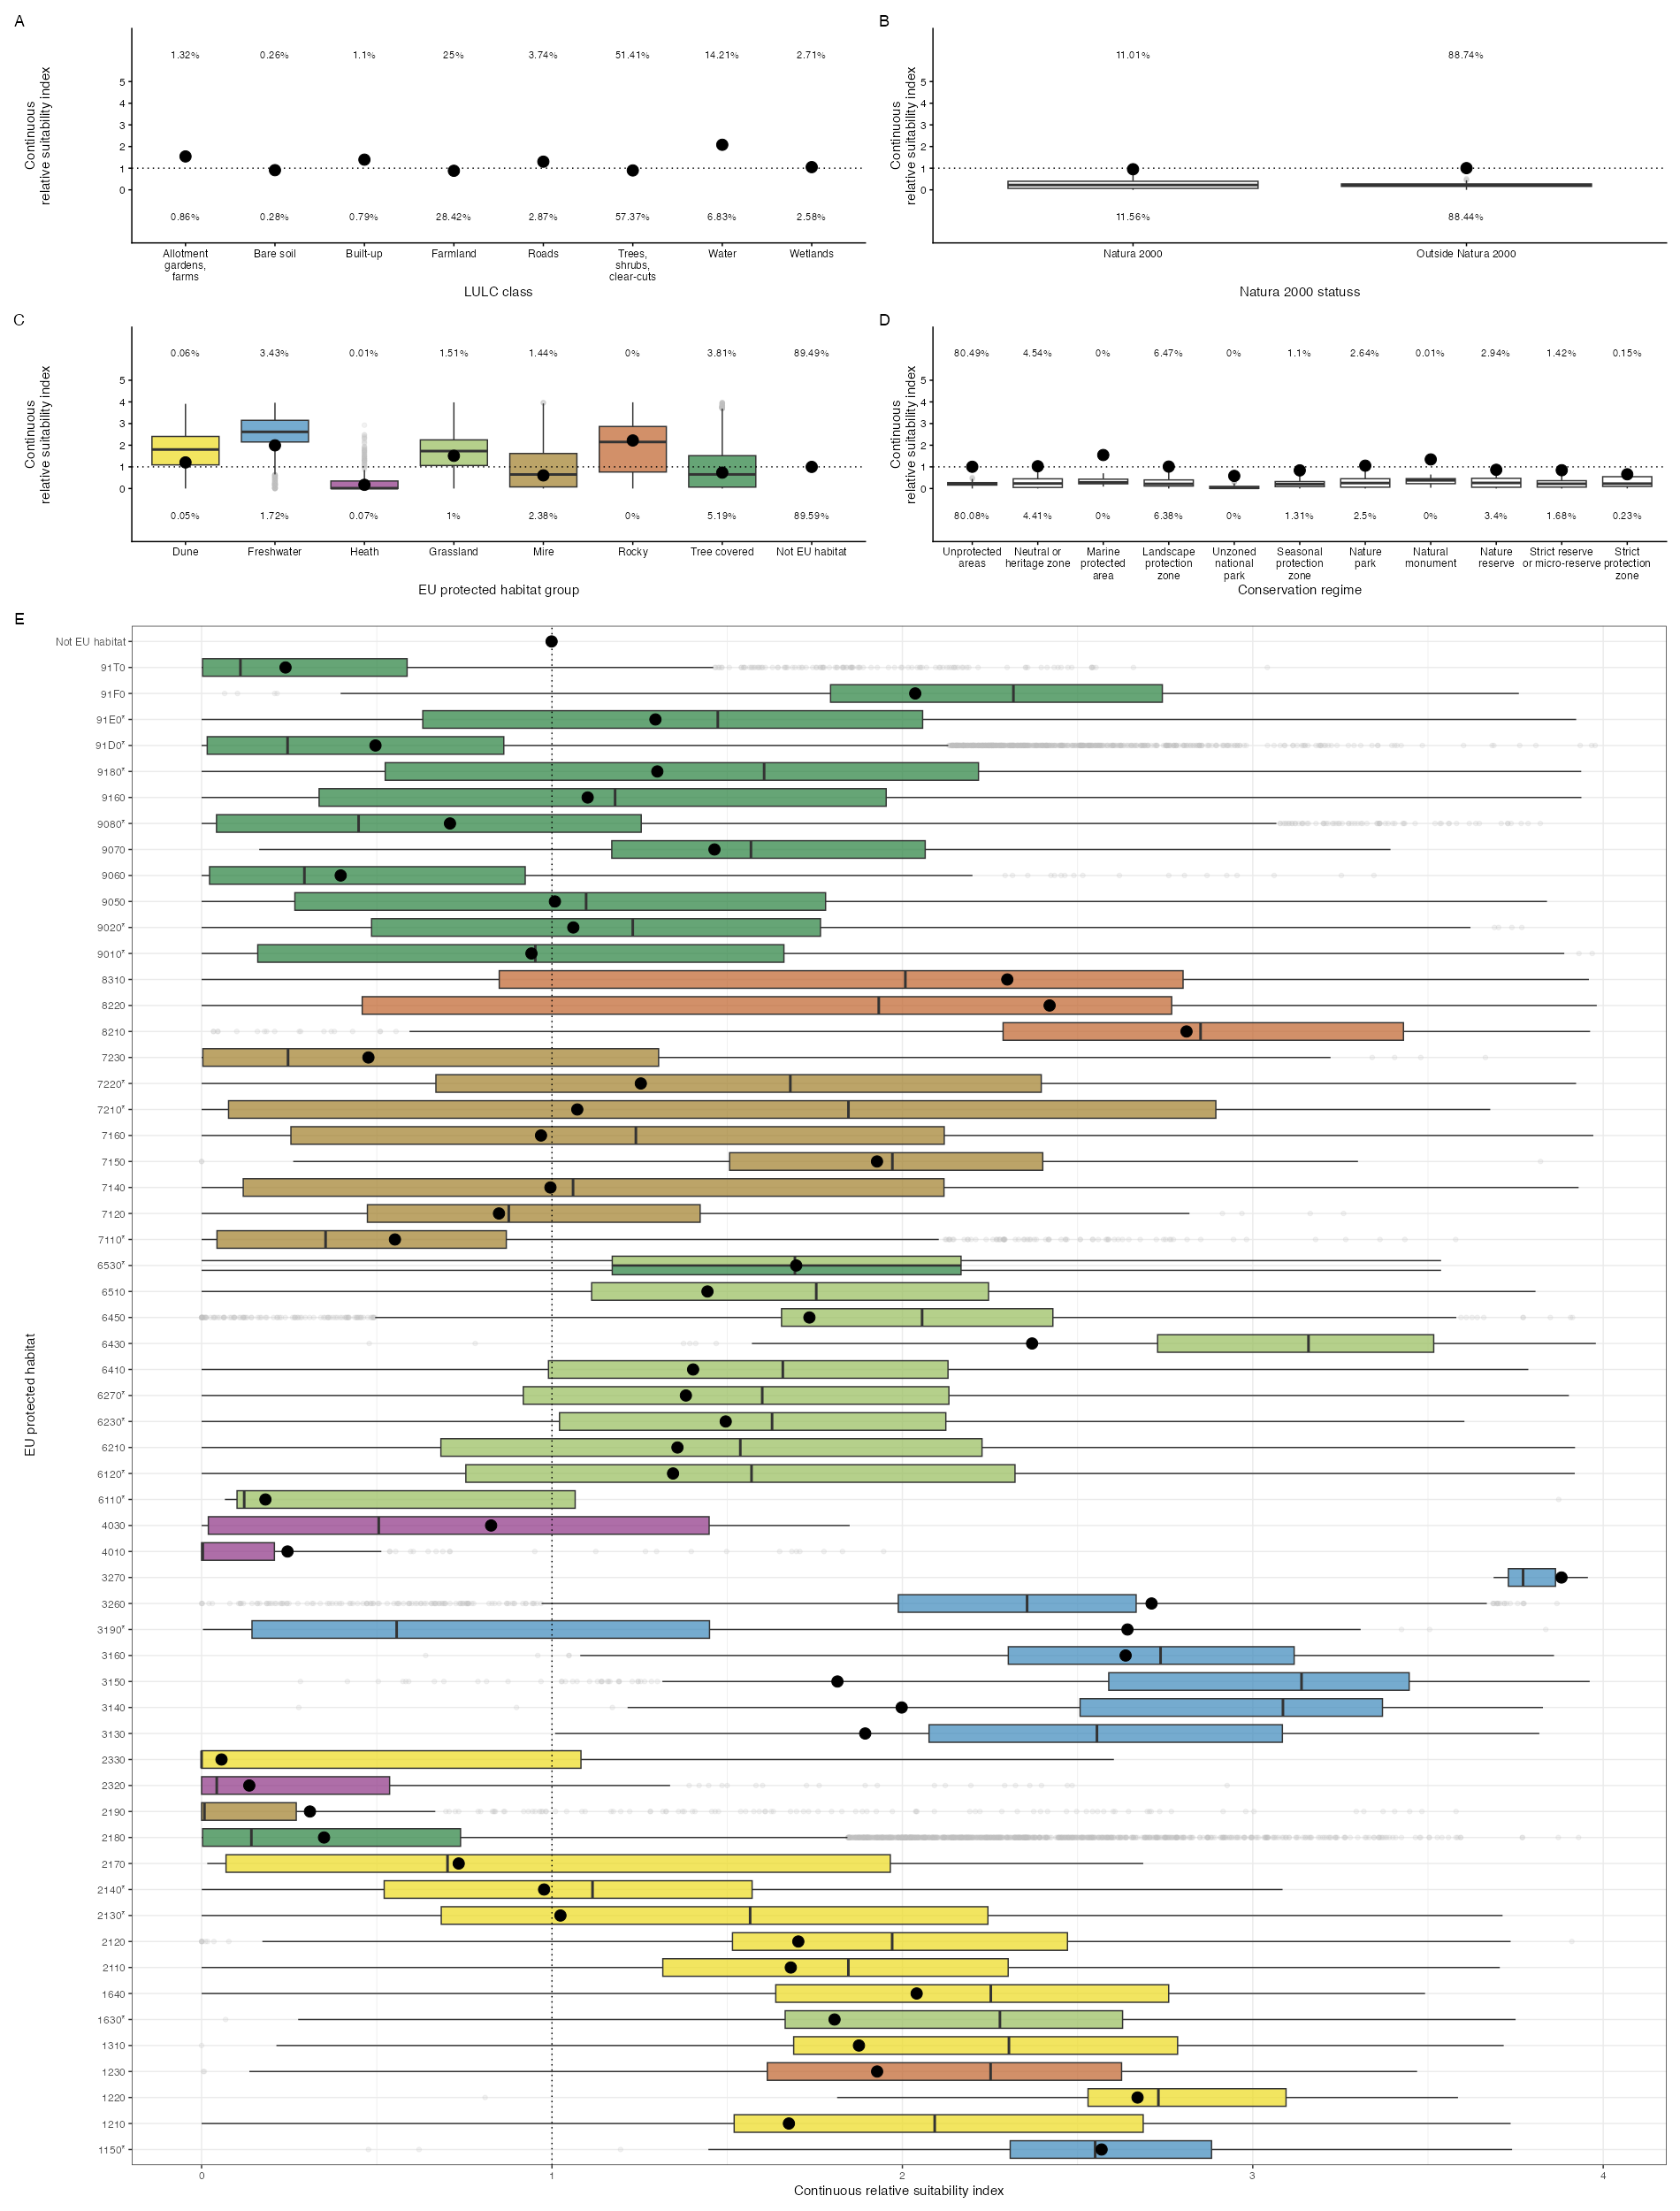
\includegraphics[width=1\linewidth,height=0.70\textheight,keepaspectratio]{results/BUFBUFmonitoringv2b5celi/PicAssoc_BUFBUFmonitoring.png}

\par\small\textit{Associations between predicted suitability and: (A) land use land cover classes, (B) Natura 2000 status, (C) stratified EU protected habitat classes, (D) conservation regime, and (E) EU protected habitats. The y-axis show continuous relative suitability index (derivative of Manly's index of preference). Colours in (C) and (E) correspond to stratified EU protected habitat classes. For classifications composed of multiple individual polygons, polygon-level indices were additionally calculated to show within-category variation. The figures therefore combine category-level estimates (points) with the distributions of polygon-level values (boxplots, where applicable). Labels above and below the panels report, respectively, the percentage of total predicted suitability and the percentage of mapped area represented by each category. **For a full resolution refer to repository: link or online document: link**}\normalsize
\end{center}

\section*{Conservation prioritization}\label{conservation-prioritization-11}
\addcontentsline{toc}{section}{Conservation prioritization}

\begin{center}
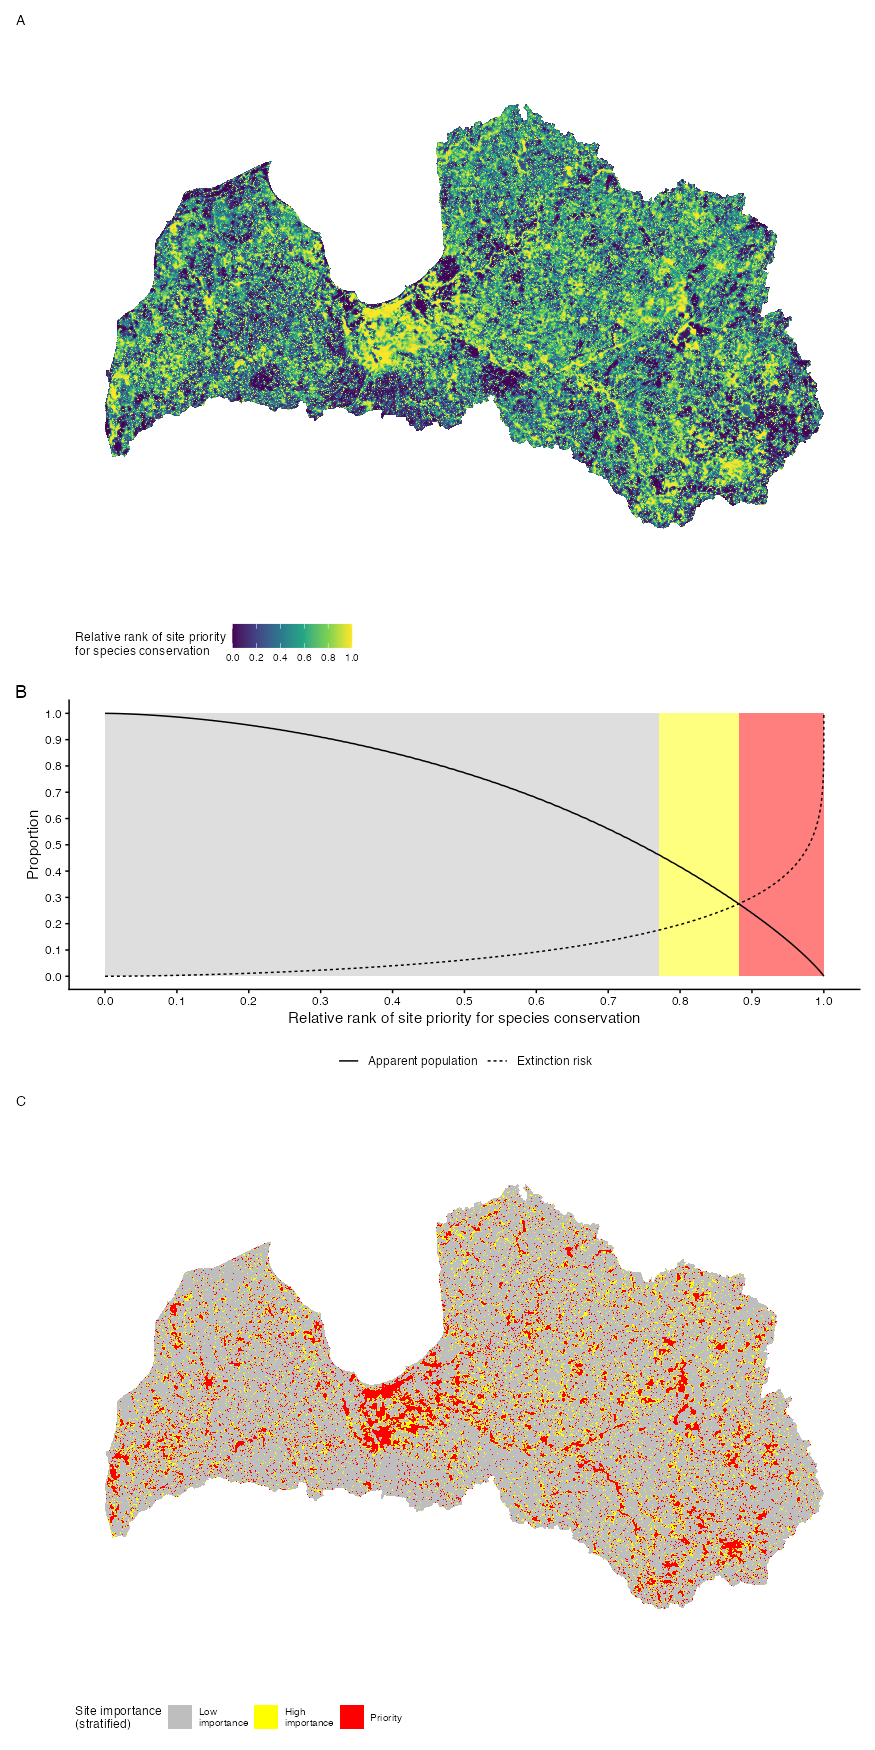
\includegraphics[width=0.85\linewidth,height=0.70\textheight,keepaspectratio]{results/BUFBUFmonitoringv2b5celi/PicPrior_BUFBUFmonitoring.png}

\par\small\textit{Single-species conservation prioritization focusing on maximisation of core area protection (CAZMAX) while accounting for site connectivity: (A) relative site rank; (B) relationship between apparent-population and extinction-risk curves with a simplified classification which is spatially demonstrated in the bootom row; (C) spatial distribution of proposed classification of site prioritization results. **For a full resolution refer to repository: link or online document: link**}\normalsize
\end{center}

\chapter*{\texorpdfstring{\emph{Bufotes viridis}}{Bufotes viridis}}\label{bufvir}
\addcontentsline{toc}{chapter}{\emph{Bufotes viridis}}

\section*{Summary}\label{summary-12}
\addcontentsline{toc}{section}{Summary}

\subsection*{Model description}\label{model-description-12}
\addcontentsline{toc}{subsection}{Model description}

Occurrence and background data were divided into model-training with four block spatial cross-validation data and an independent test set. Sampling-bias/background treatment: \textbf{Phenology Weighted Target Group}. Observations were retained only where accumulated LULC change within the 1-ha analysis cell from the year of observation to 2024 did not exceed 50\%; observations were retained only where accumulated LULC change within the home-range radius around the analysis cell from the year of observation to 2024 did not exceed 50\%.

The final data set contained \textbf{67} presence records: \textbf{50} for training with four spatial block cross-validation and \textbf{17} for independent testing. Training background contained \textbf{29858} locations, with \textbf{10142} additional independent-test background locations.

\subsection*{Expert assessment scores}\label{expert-assessment-scores-12}
\addcontentsline{toc}{subsection}{Expert assessment scores}

\begin{itemize}
\tightlist
\item
  \textbf{Marginal responses and variable importance score:} 3 (moderate ecological interpretability)
\item
  \textbf{Map score:} 4 (good agreement with known distribution)
\item
  \textbf{Applicability score:} 3 (moderate applicability)
\end{itemize}

\textbf{Šo sadaļu aizpildām manuāli no ekspertu aptaujām}

\subsection*{Statistical evaluation}\label{statistical-evaluation-12}
\addcontentsline{toc}{subsection}{Statistical evaluation}

The final model had a training TSS of \textbf{0.401}, with a training-derived cloglog threshold of \textbf{0.431}. Combined training AUC was \textbf{0.926} and combined test AUC was \textbf{0.874}.

\subsubsection*{Spatial cross-validation}\label{spatial-cross-validation-12}
\addcontentsline{toc}{subsubsection}{Spatial cross-validation}

\begin{itemize}
\tightlist
\item
  \textbf{AUC:} 0.8496 ± 0.0701; null models: 0.5326 ± 0.0586; z = 5.406, p \textless{} 0.001
\item
  \textbf{CBI:} 0.7868 ± 0.0332; null models: -0.0333 ± 0.1805; z = 4.5443, p \textless{} 0.001
\item
  \textbf{OR10:} 0.3494 ± 0.2517; null models: 0.2724 ± 0.133; z = 0.5788, p = 0.719
\item
  \textbf{ORmin:} 0.1635 ± 0.1362; null models: 0.109 ± 0.105; z = 0.5182, p = 0.698
\end{itemize}

\subsubsection*{Independent testing}\label{independent-testing-12}
\addcontentsline{toc}{subsubsection}{Independent testing}

\begin{itemize}
\tightlist
\item
  \textbf{TSS:} 0.446; \textbf{sensitivity:} 0.588; \textbf{specificity:} 0.857
\item
  \textbf{AUC:} 0.856; null models: 0.5031 ± 0.1331; z = 2.6524, p = 0.004
\item
  \textbf{CBI:} 0.721; null models: -0.0338 ± 0.4556; z = 1.6566, p = 0.049
\item
  \textbf{OR10:} 0.412; null models: 0.2418 ± 0.1651; z = 1.0297, p = 0.848
\item
  \textbf{ORmin:} 0.059; null models: 0.0582 ± 0.0895; z = 0.0066, p = 0.503
\end{itemize}

\subsection*{Conservation prioritisation summary}\label{conservation-prioritisation-summary-12}
\addcontentsline{toc}{subsection}{Conservation prioritisation summary}

The primary priority area covers \textbf{4.6\%} of Latvia and contains \textbf{27.5\%} of the summed habitat suitability (apparent population proxy).

The broader high importance area covers \textbf{8.2\%} of Latvia and contains \textbf{40.9\%} of the summed habitat suitability.

For comparison, the area classified as suitable using the maximum training sensitivity plus specificity habitat-suitability threshold contains \textbf{40.9\%} of the summed continuous habitat suitability.

\subsection*{Version evolution}\label{version-evolution-12}
\addcontentsline{toc}{subsection}{Version evolution}

\textbf{Šo sadaļu aizpildām manuāli, izmntojot sagatavotās shēmas. Jāvienojas par to noformējumu}

\section*{Habitat suitability}\label{habitat-suitability-12}
\addcontentsline{toc}{section}{Habitat suitability}

\begin{center}
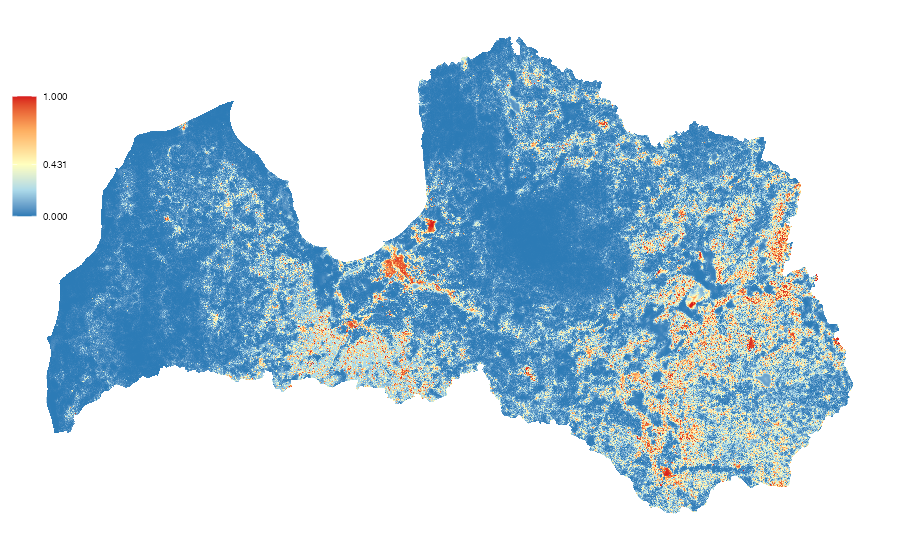
\includegraphics[width=1\linewidth,height=0.70\textheight,keepaspectratio]{results/BUFVIRv2a1_2025/PicHSmap_BUFVIR.png}

\par\small\textit{Predicted continuous habitat suitability across Latvia. The warmer the colour the higher is the predicted habitat suitability. Value in the middle of the legend correspond to the maximum training sensitivity plus specificity threshold. **For a full resolution refer to repository: link or online document: link**}\normalsize
\end{center}

\section*{Model thresholds}\label{model-thresholds-12}
\addcontentsline{toc}{section}{Model thresholds}

Threshold values and associated omission rates

\begin{center}
\resizebox{\linewidth}{!}{%

\begin{tabular}{lrrrrr}
\toprule
Threshold & Cloglog value & Fractional predicted area & Training omission rate & Test omission rate & P-values\\
\midrule
Minimum training presence & 0.1749707 & 0.3585013 & 0.00 & 0.0000984 & 0\\
Equal training sensitivity and specificity & 0.4967938 & 0.1452488 & 0.14 & 0.0006890 & 0\\
Maximum training sensitivity plus specificity & 0.4308510 & 0.1724369 & 0.08 & 0.0006890 & 0\\
Equal test sensitivity and specificity & 0.2453485 & 0.2876515 & 0.02 & 0.0003937 & 0\\
Maximum test sensitivity plus specificity & 0.1654343 & 0.3698855 & 0.00 & 0.0000000 & 0\\
\bottomrule
\end{tabular}
}
\end{center}

\section*{Variable importance}\label{variable-importance-12}
\addcontentsline{toc}{section}{Variable importance}

\begin{center}
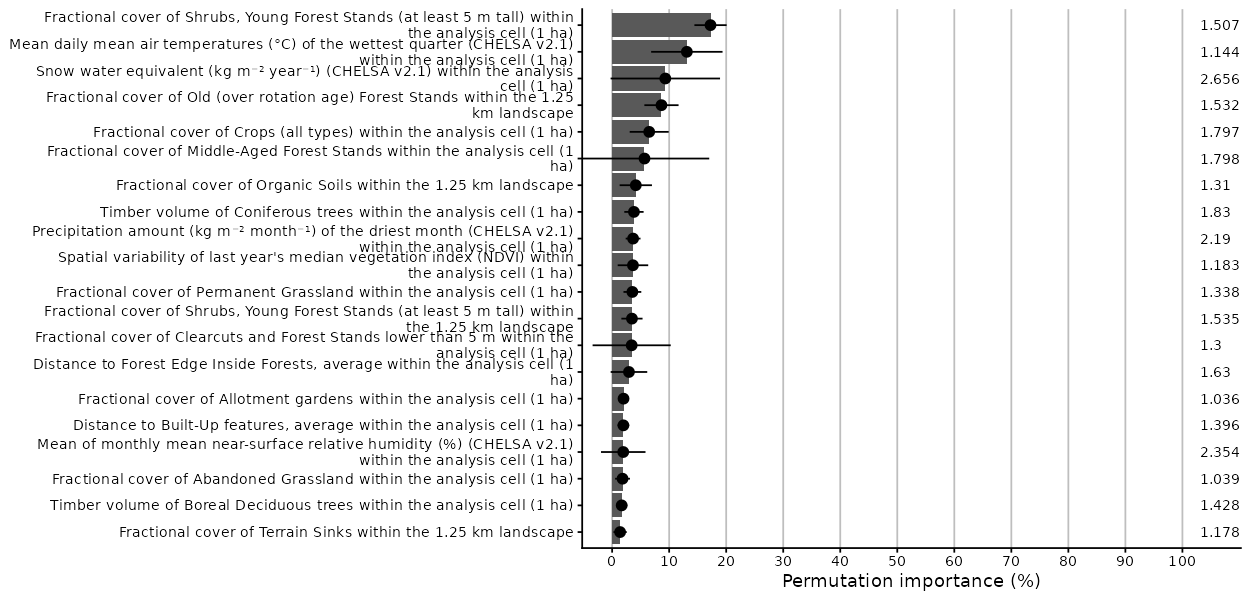
\includegraphics[width=1\linewidth,height=0.70\textheight,keepaspectratio]{results/BUFVIRv2a1_2025/PicVarImpVIFs_BUFVIR.png}

\par\small\textit{Permutation-importance (mean and standard deviation from 99 permutations, on the x-axis) of the ecogeographical variables (first y-axis, left side), and their variance inflation factor values (second y-axis, right side). **For a full resolution refer to repository: link or online document: link**}\normalsize
\end{center}

\section*{Marginal responses}\label{marginal-responses-12}
\addcontentsline{toc}{section}{Marginal responses}

\begin{center}
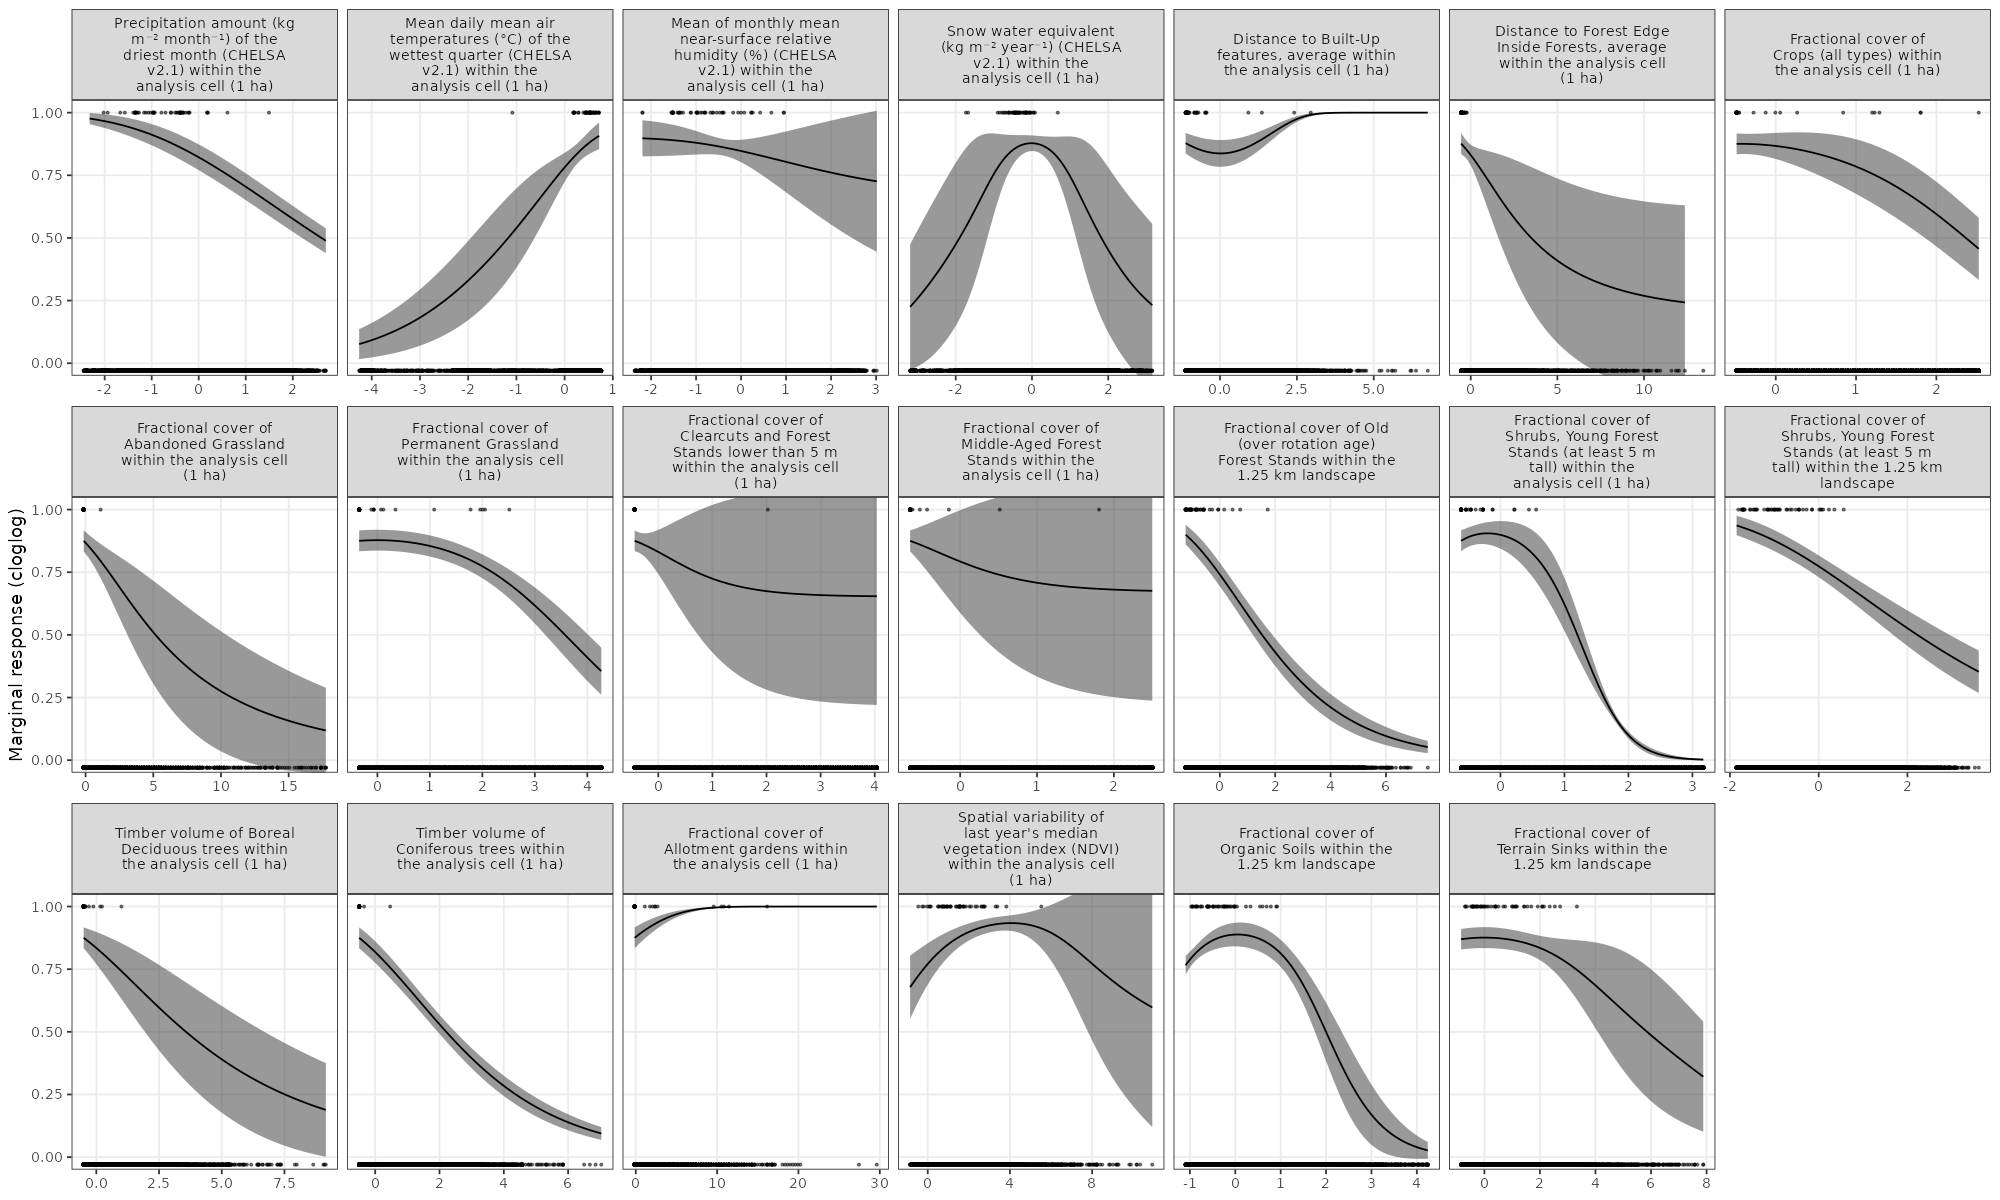
\includegraphics[width=1\linewidth,height=0.70\textheight,keepaspectratio]{results/BUFVIRv2a1_2025/PicMargResp_BUFVIR.png}

\par\small\textit{Marginalised for arithmetic mean response curves illustrating the effect of each ecogeographical variable on the habitat suitability when all the other variables have their arithmetic mean values. The y-axis shows the predicted habitat suitability (cloglog-transformed), while the x-axis shows the standardised (centred and scaled) value of the ecogeographical variable. Dots at a value of 1 on the y-axis illustrate presence locations in the environment (on the x-axis), while dots at a value of 0 illustrate background locations used in modelling.  **For a full resolution refer to repository: link or online document: link**}\normalsize
\end{center}

\section*{Habitat and conservation associations}\label{habitat-and-conservation-associations-12}
\addcontentsline{toc}{section}{Habitat and conservation associations}

\begin{center}
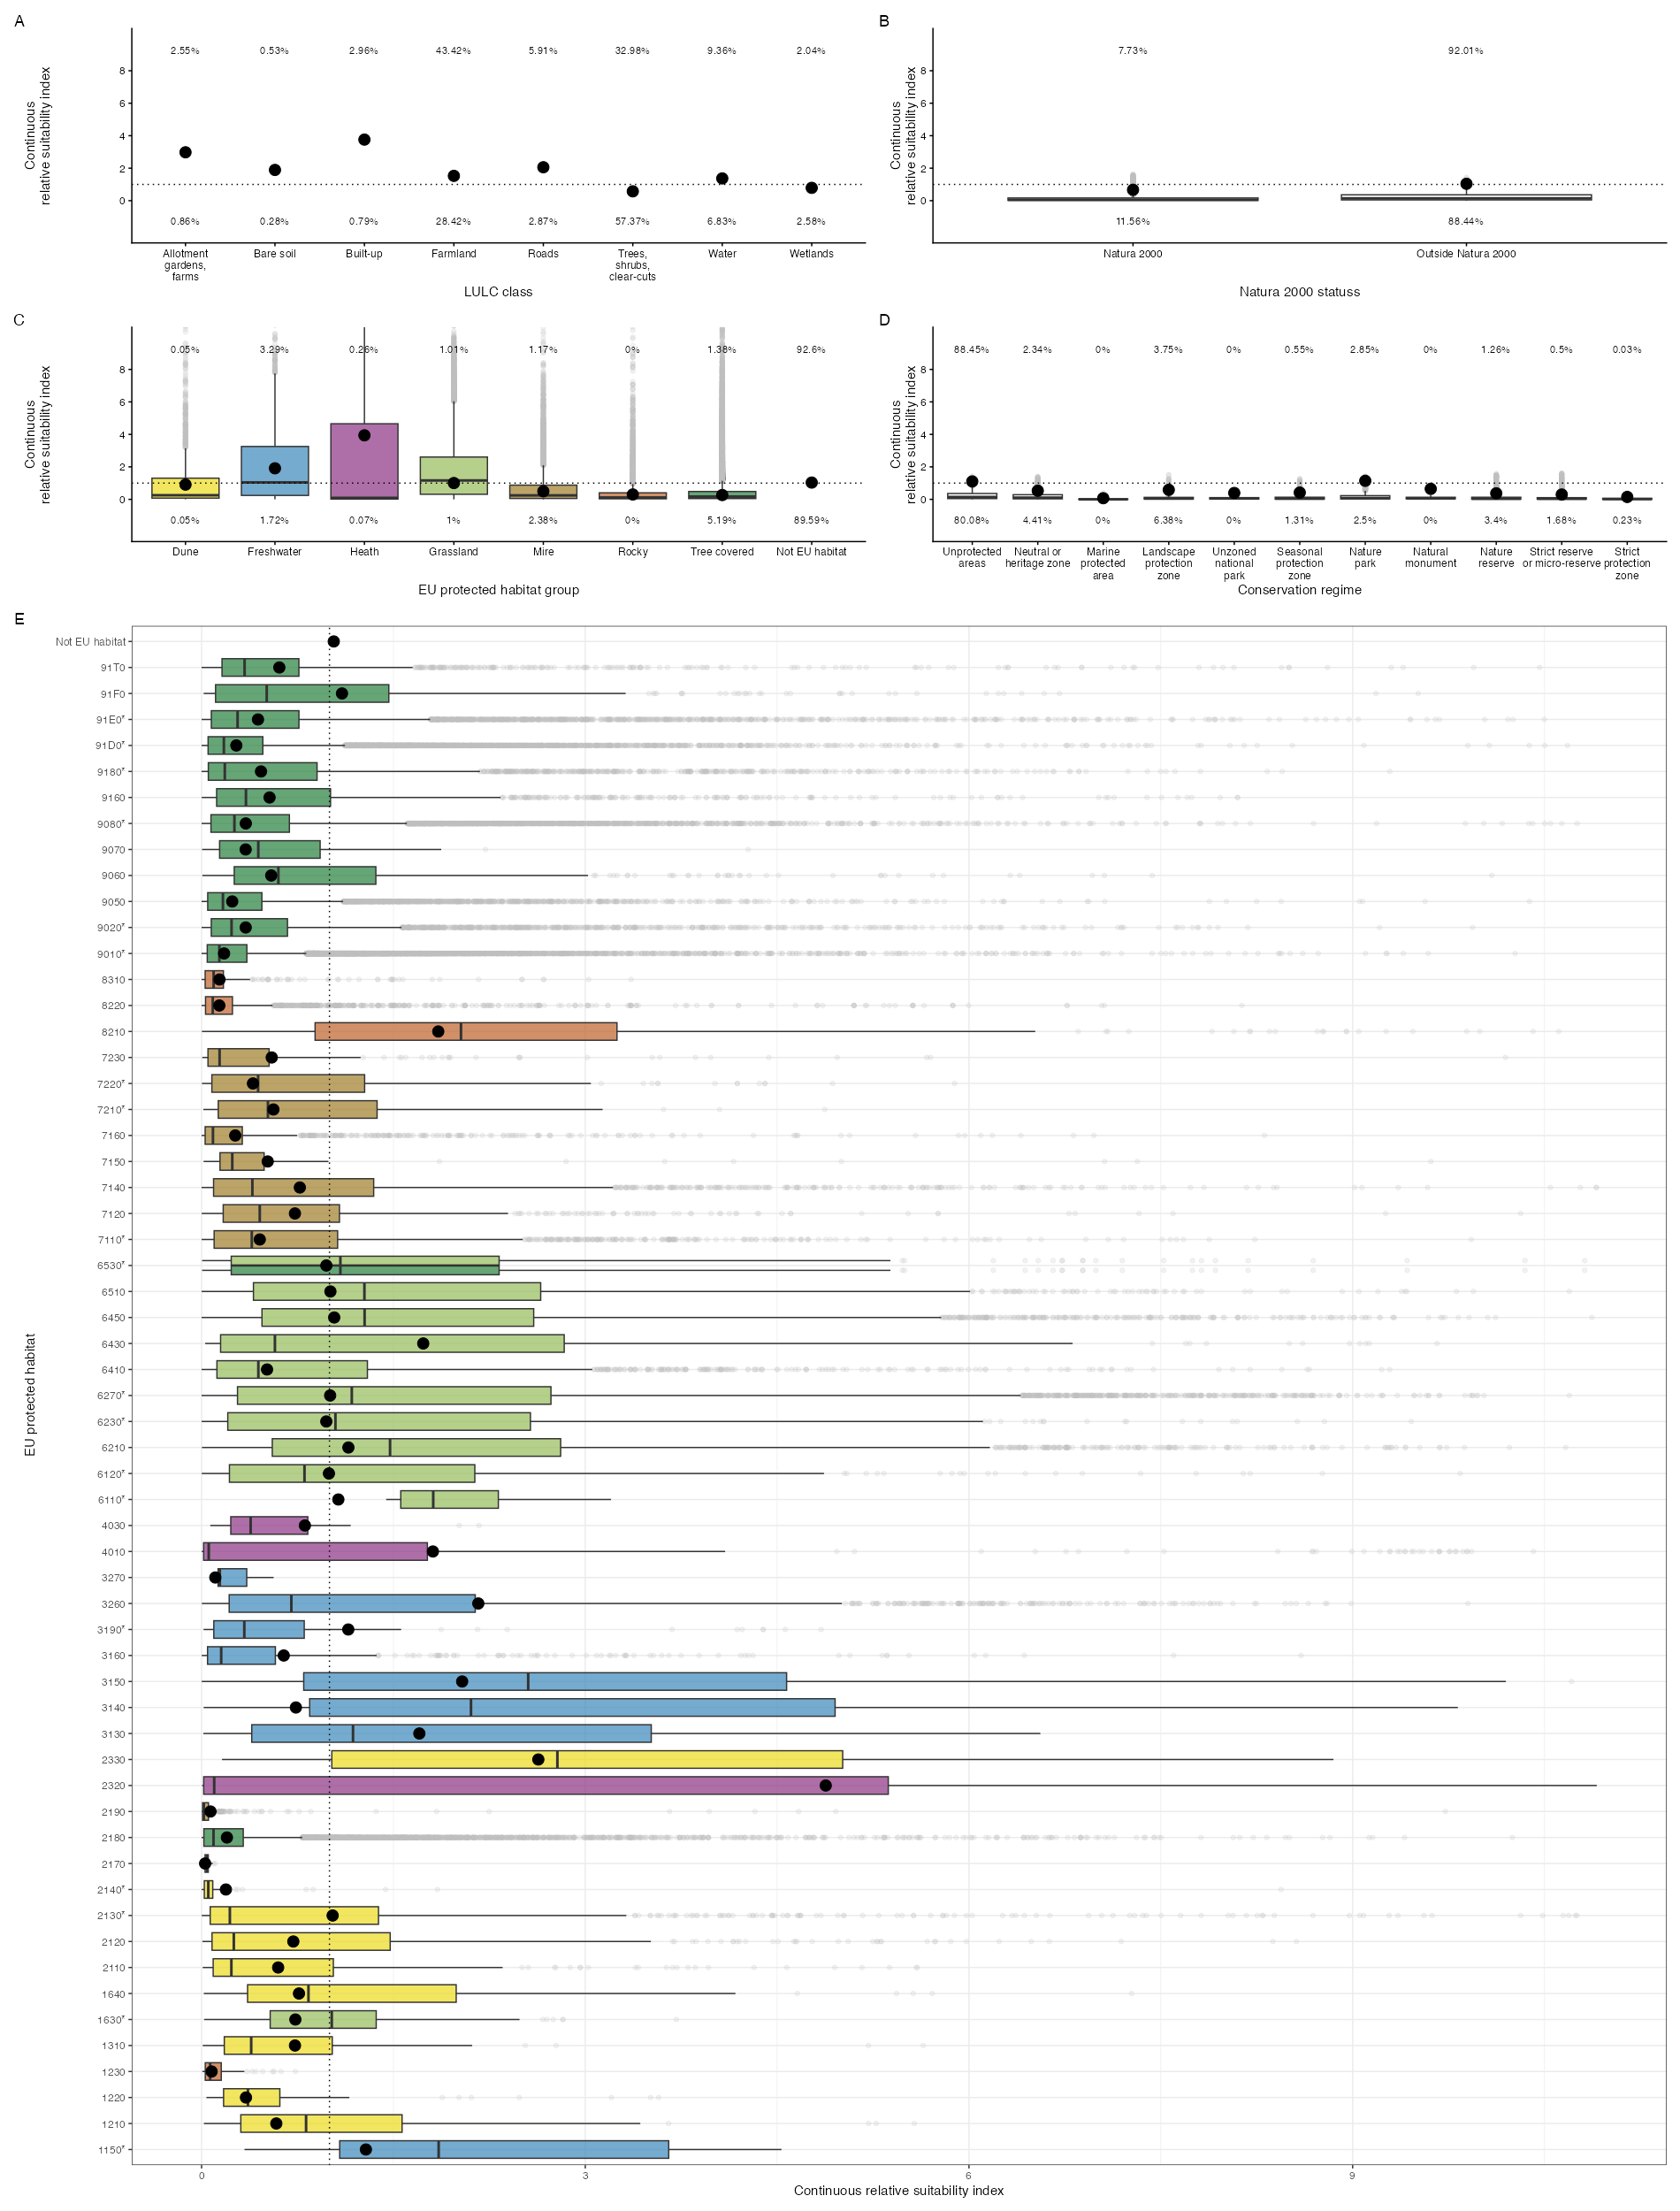
\includegraphics[width=1\linewidth,height=0.70\textheight,keepaspectratio]{results/BUFVIRv2a1_2025/PicAssoc_BUFVIR.png}

\par\small\textit{Associations between predicted suitability and: (A) land use land cover classes, (B) Natura 2000 status, (C) stratified EU protected habitat classes, (D) conservation regime, and (E) EU protected habitats. The y-axis show continuous relative suitability index (derivative of Manly's index of preference). Colours in (C) and (E) correspond to stratified EU protected habitat classes. For classifications composed of multiple individual polygons, polygon-level indices were additionally calculated to show within-category variation. The figures therefore combine category-level estimates (points) with the distributions of polygon-level values (boxplots, where applicable). Labels above and below the panels report, respectively, the percentage of total predicted suitability and the percentage of mapped area represented by each category. **For a full resolution refer to repository: link or online document: link**}\normalsize
\end{center}

\section*{Conservation prioritization}\label{conservation-prioritization-12}
\addcontentsline{toc}{section}{Conservation prioritization}

\begin{center}
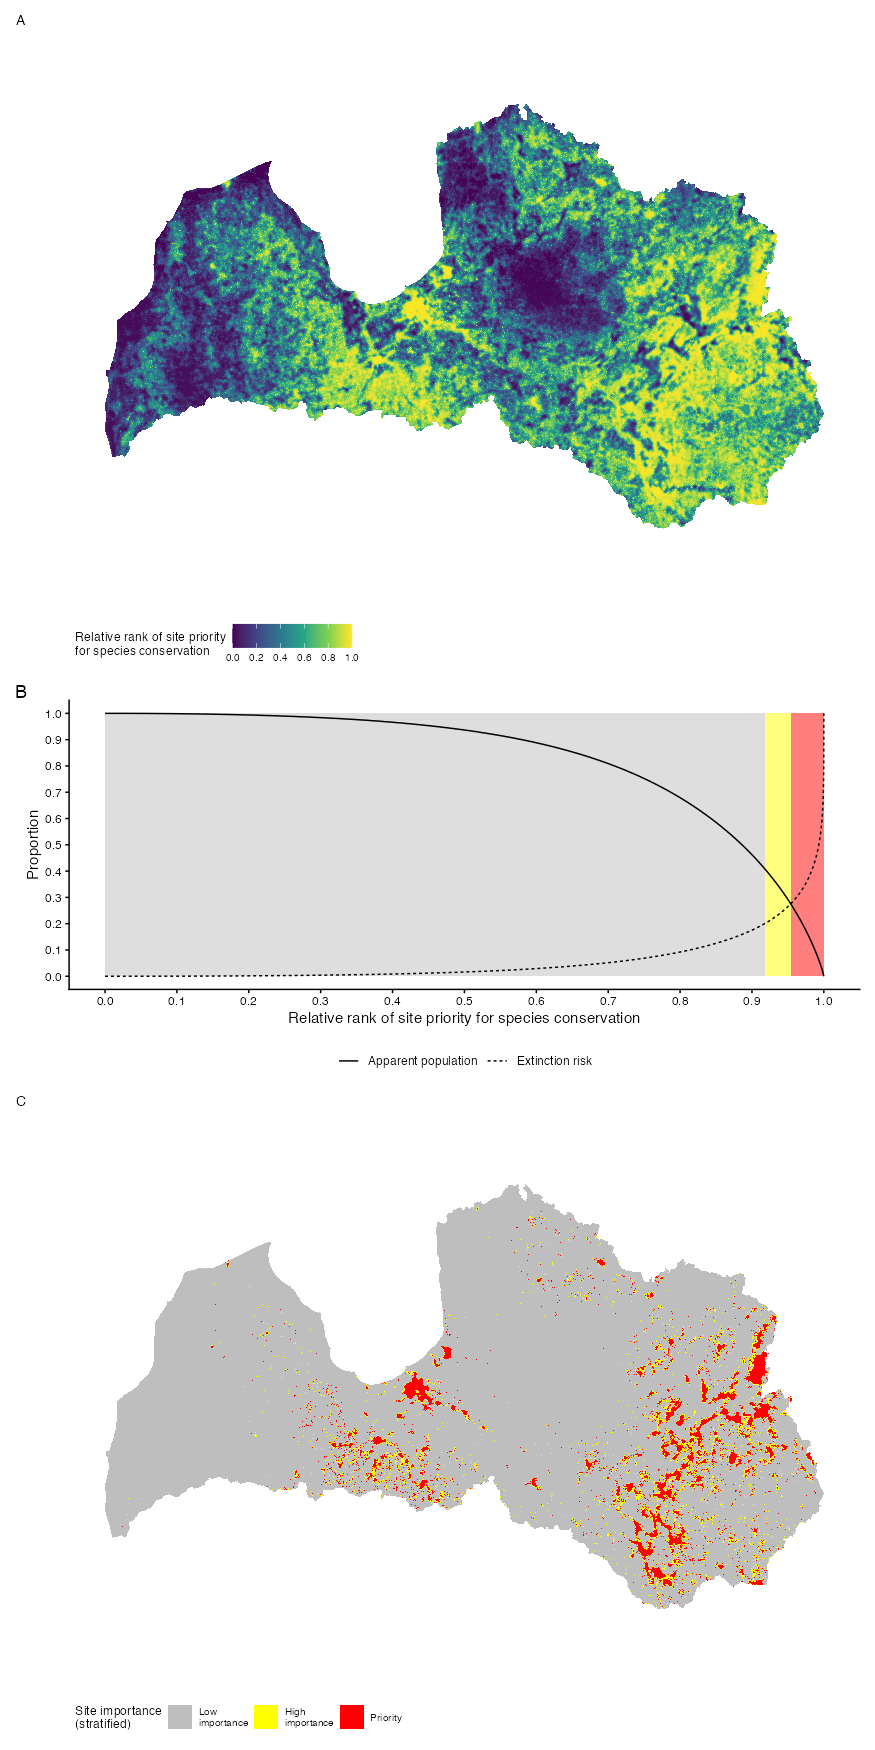
\includegraphics[width=0.85\linewidth,height=0.70\textheight,keepaspectratio]{results/BUFVIRv2a1_2025/PicPrior_BUFVIR.png}

\par\small\textit{Single-species conservation prioritization focusing on maximisation of core area protection (CAZMAX) while accounting for site connectivity: (A) relative site rank; (B) relationship between apparent-population and extinction-risk curves with a simplified classification which is spatially demonstrated in the bootom row; (C) spatial distribution of proposed classification of site prioritization results. **For a full resolution refer to repository: link or online document: link**}\normalsize
\end{center}

\chapter*{\texorpdfstring{\emph{Hyla orientalis}}{Hyla orientalis}}\label{hylori}
\addcontentsline{toc}{chapter}{\emph{Hyla orientalis}}

\section*{Summary}\label{summary-13}
\addcontentsline{toc}{section}{Summary}

\subsection*{Model description}\label{model-description-13}
\addcontentsline{toc}{subsection}{Model description}

Occurrence and background data were divided into model-training with four block spatial cross-validation data and an independent test set. Sampling-bias/background treatment: \textbf{Phenology Weighted Target Group}. Accumulated LULC change within the 1-ha analysis cell was not evaluated; accumulated LULC change within the home-range radius around the analysis cell was not evaluated.

The final data set contained \textbf{323} presence records: \textbf{242} for training with four spatial block cross-validation and \textbf{81} for independent testing. Training background contained \textbf{29973} locations, with \textbf{10027} additional independent-test background locations.

\subsection*{Expert assessment scores}\label{expert-assessment-scores-13}
\addcontentsline{toc}{subsection}{Expert assessment scores}

\begin{itemize}
\tightlist
\item
  \textbf{Marginal responses and variable importance score:} 3 (moderate ecological interpretability)
\item
  \textbf{Map score:} 3 (moderate agreement with known distribution)
\item
  \textbf{Applicability score:} 3 (moderate applicability)
\end{itemize}

\textbf{Šo sadaļu aizpildām manuāli no ekspertu aptaujām}

\subsection*{Statistical evaluation}\label{statistical-evaluation-13}
\addcontentsline{toc}{subsection}{Statistical evaluation}

The final model had a training TSS of \textbf{0.401}, with a training-derived cloglog threshold of \textbf{0.165}. Combined training AUC was \textbf{0.934} and combined test AUC was \textbf{0.913}.

\subsubsection*{Spatial cross-validation}\label{spatial-cross-validation-13}
\addcontentsline{toc}{subsubsection}{Spatial cross-validation}

\begin{itemize}
\tightlist
\item
  \textbf{AUC:} 0.8675 ± 0.104; null models: 0.6991 ± 0.0263; z = 6.4151, p \textless{} 0.001
\item
  \textbf{CBI:} 0.8852 ± 0.0611; null models: 0.2863 ± 0.1803; z = 3.3224, p \textless{} 0.001
\item
  \textbf{OR10:} 0.1818 ± 0.1205; null models: 0.0041 ± 0.0151; z = 11.8039, p = 1
\item
  \textbf{ORmin:} 0.037 ± 0.0542; null models: 5e-04 ± 0.0053; z = 6.8808, p = 1
\end{itemize}

\subsubsection*{Independent testing}\label{independent-testing-13}
\addcontentsline{toc}{subsubsection}{Independent testing}

\begin{itemize}
\tightlist
\item
  \textbf{TSS:} 0.68; \textbf{sensitivity:} 0.938; \textbf{specificity:} 0.742
\item
  \textbf{AUC:} 0.924; null models: 0.5356 ± 0.159; z = 2.4448, p = 0.007
\item
  \textbf{CBI:} 0.939; null models: 0.0858 ± 0.6135; z = 1.3907, p = 0.082
\item
  \textbf{OR10:} 0.111; null models: 0.1765 ± 0.1524; z = -0.4294, p = 0.334
\item
  \textbf{ORmin:} 0.012; null models: 0.01 ± 0.0175; z = 0.1339, p = 0.553
\end{itemize}

\subsection*{Conservation prioritisation summary}\label{conservation-prioritisation-summary-13}
\addcontentsline{toc}{subsection}{Conservation prioritisation summary}

The primary priority area covers \textbf{1.6\%} of Latvia and contains \textbf{27.6\%} of the summed habitat suitability (apparent population proxy).

The broader high importance area covers \textbf{8.1\%} of Latvia and contains \textbf{79.6\%} of the summed habitat suitability.

For comparison, the area classified as suitable using the maximum training sensitivity plus specificity habitat-suitability threshold contains \textbf{79.6\%} of the summed continuous habitat suitability.

\subsection*{Version evolution}\label{version-evolution-13}
\addcontentsline{toc}{subsection}{Version evolution}

\textbf{Šo sadaļu aizpildām manuāli, izmntojot sagatavotās shēmas. Jāvienojas par to noformējumu}

\section*{Habitat suitability}\label{habitat-suitability-13}
\addcontentsline{toc}{section}{Habitat suitability}

\begin{center}
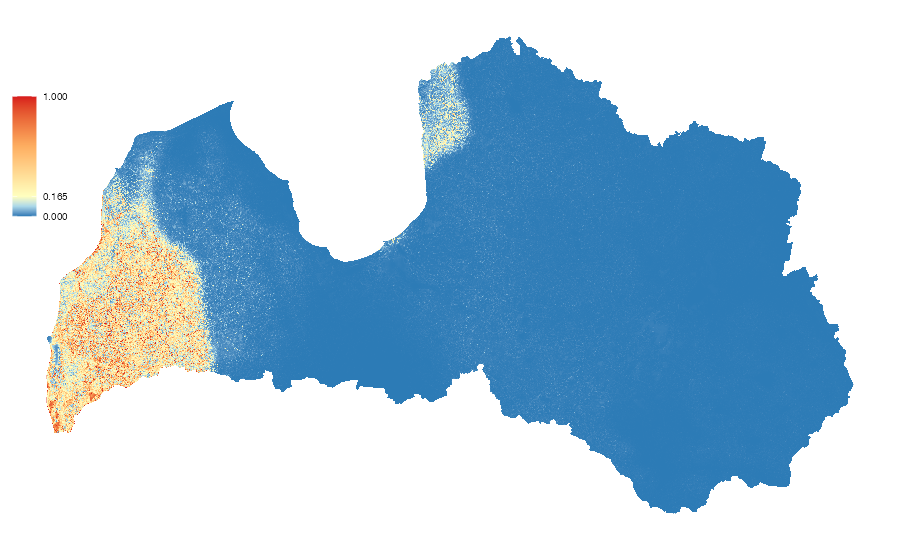
\includegraphics[width=1\linewidth,height=0.70\textheight,keepaspectratio]{results/HYLORIv4b1_2025/PicHSmap_HYLORI.png}

\par\small\textit{Predicted continuous habitat suitability across Latvia. The warmer the colour the higher is the predicted habitat suitability. Value in the middle of the legend correspond to the maximum training sensitivity plus specificity threshold. **For a full resolution refer to repository: link or online document: link**}\normalsize
\end{center}

\section*{Model thresholds}\label{model-thresholds-13}
\addcontentsline{toc}{section}{Model thresholds}

Threshold values and associated omission rates

\begin{center}
\resizebox{\linewidth}{!}{%

\begin{tabular}{lrrrrr}
\toprule
Threshold & Cloglog value & Fractional predicted area & Training omission rate & Test omission rate & P-values\\
\midrule
Minimum training presence & 0.0969671 & 0.2827850 & 0.0000000 & 0.0000986 & 0\\
Equal training sensitivity and specificity & 0.3264396 & 0.1484879 & 0.1487603 & 0.0012822 & 0\\
Maximum training sensitivity plus specificity & 0.1653129 & 0.2327684 & 0.0289256 & 0.0004931 & 0\\
Equal test sensitivity and specificity & 0.3362293 & 0.1434364 & 0.1570248 & 0.0012822 & 0\\
Maximum test sensitivity plus specificity & 0.1523717 & 0.2415753 & 0.0289256 & 0.0001973 & 0\\
\bottomrule
\end{tabular}
}
\end{center}

\section*{Variable importance}\label{variable-importance-13}
\addcontentsline{toc}{section}{Variable importance}

\begin{center}
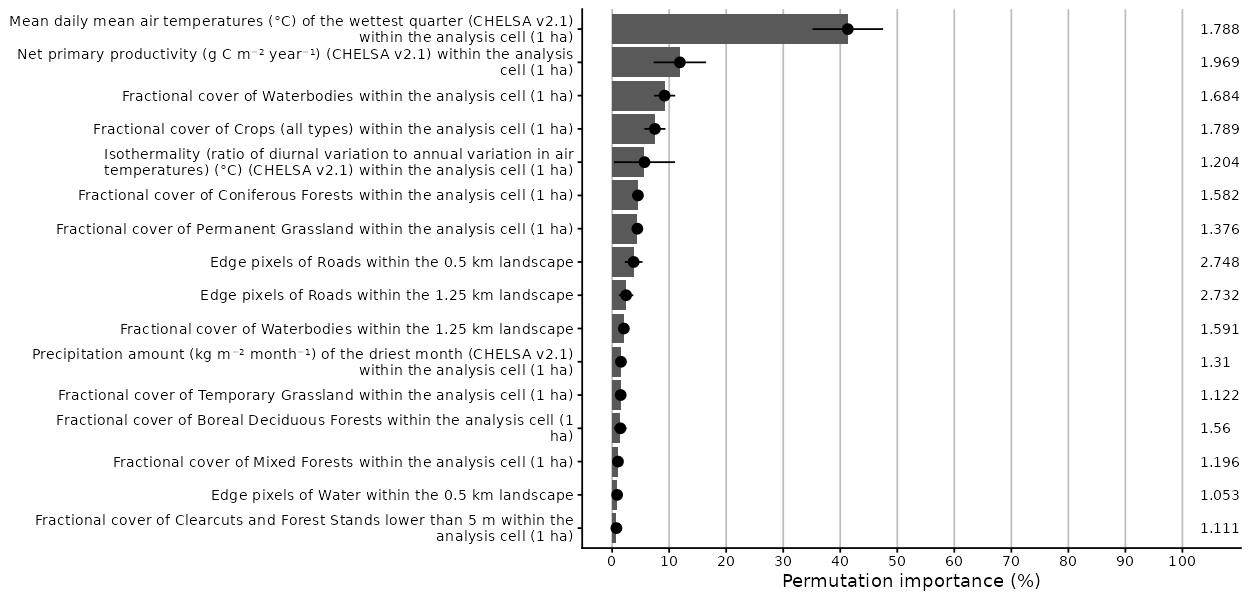
\includegraphics[width=1\linewidth,height=0.70\textheight,keepaspectratio]{results/HYLORIv4b1_2025/PicVarImpVIFs_HYLORI.png}

\par\small\textit{Permutation-importance (mean and standard deviation from 99 permutations, on the x-axis) of the ecogeographical variables (first y-axis, left side), and their variance inflation factor values (second y-axis, right side). **For a full resolution refer to repository: link or online document: link**}\normalsize
\end{center}

\section*{Marginal responses}\label{marginal-responses-13}
\addcontentsline{toc}{section}{Marginal responses}

\begin{center}
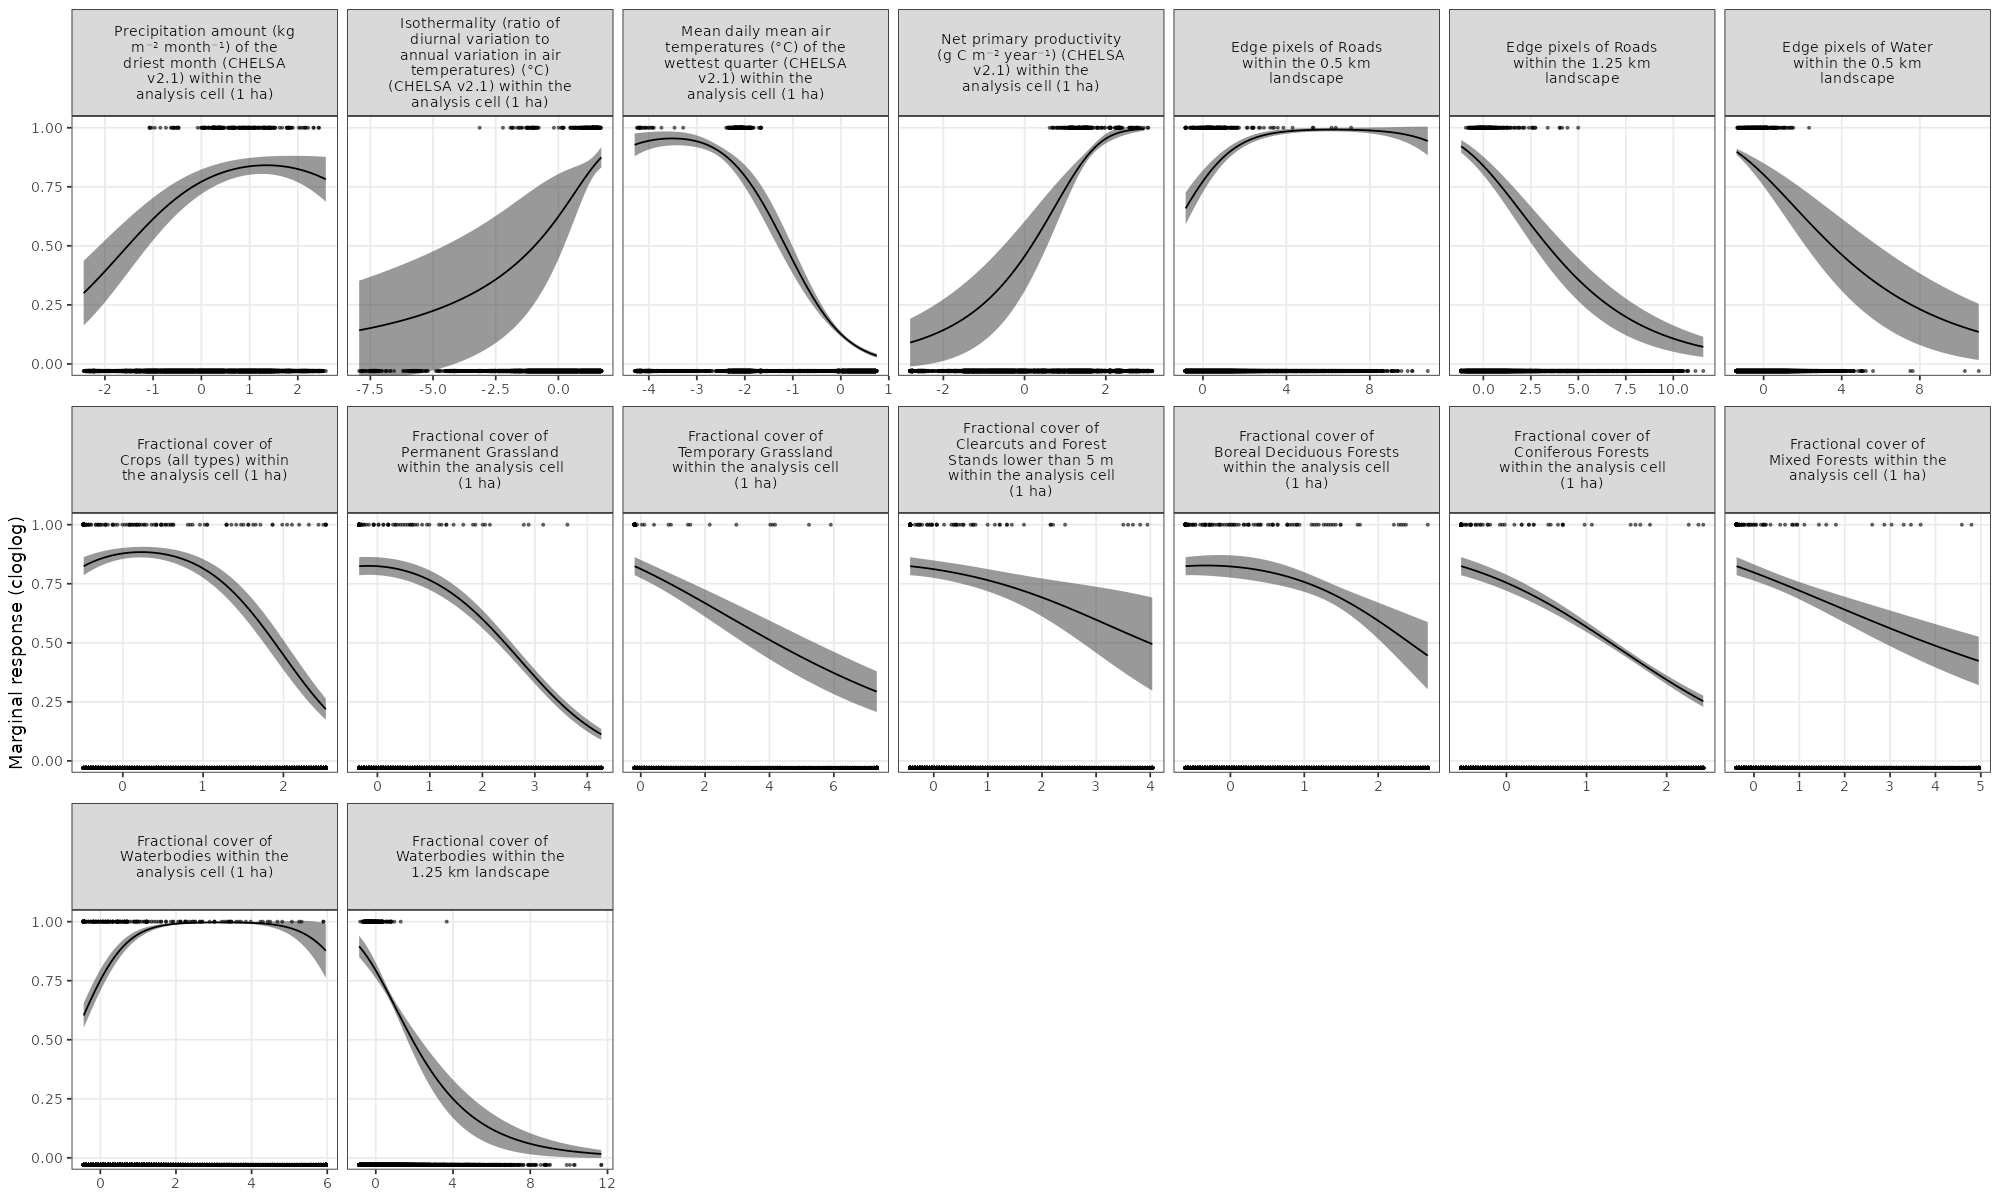
\includegraphics[width=1\linewidth,height=0.70\textheight,keepaspectratio]{results/HYLORIv4b1_2025/PicMargResp_HYLORI.png}

\par\small\textit{Marginalised for arithmetic mean response curves illustrating the effect of each ecogeographical variable on the habitat suitability when all the other variables have their arithmetic mean values. The y-axis shows the predicted habitat suitability (cloglog-transformed), while the x-axis shows the standardised (centred and scaled) value of the ecogeographical variable. Dots at a value of 1 on the y-axis illustrate presence locations in the environment (on the x-axis), while dots at a value of 0 illustrate background locations used in modelling.  **For a full resolution refer to repository: link or online document: link**}\normalsize
\end{center}

\section*{Habitat and conservation associations}\label{habitat-and-conservation-associations-13}
\addcontentsline{toc}{section}{Habitat and conservation associations}

\begin{center}
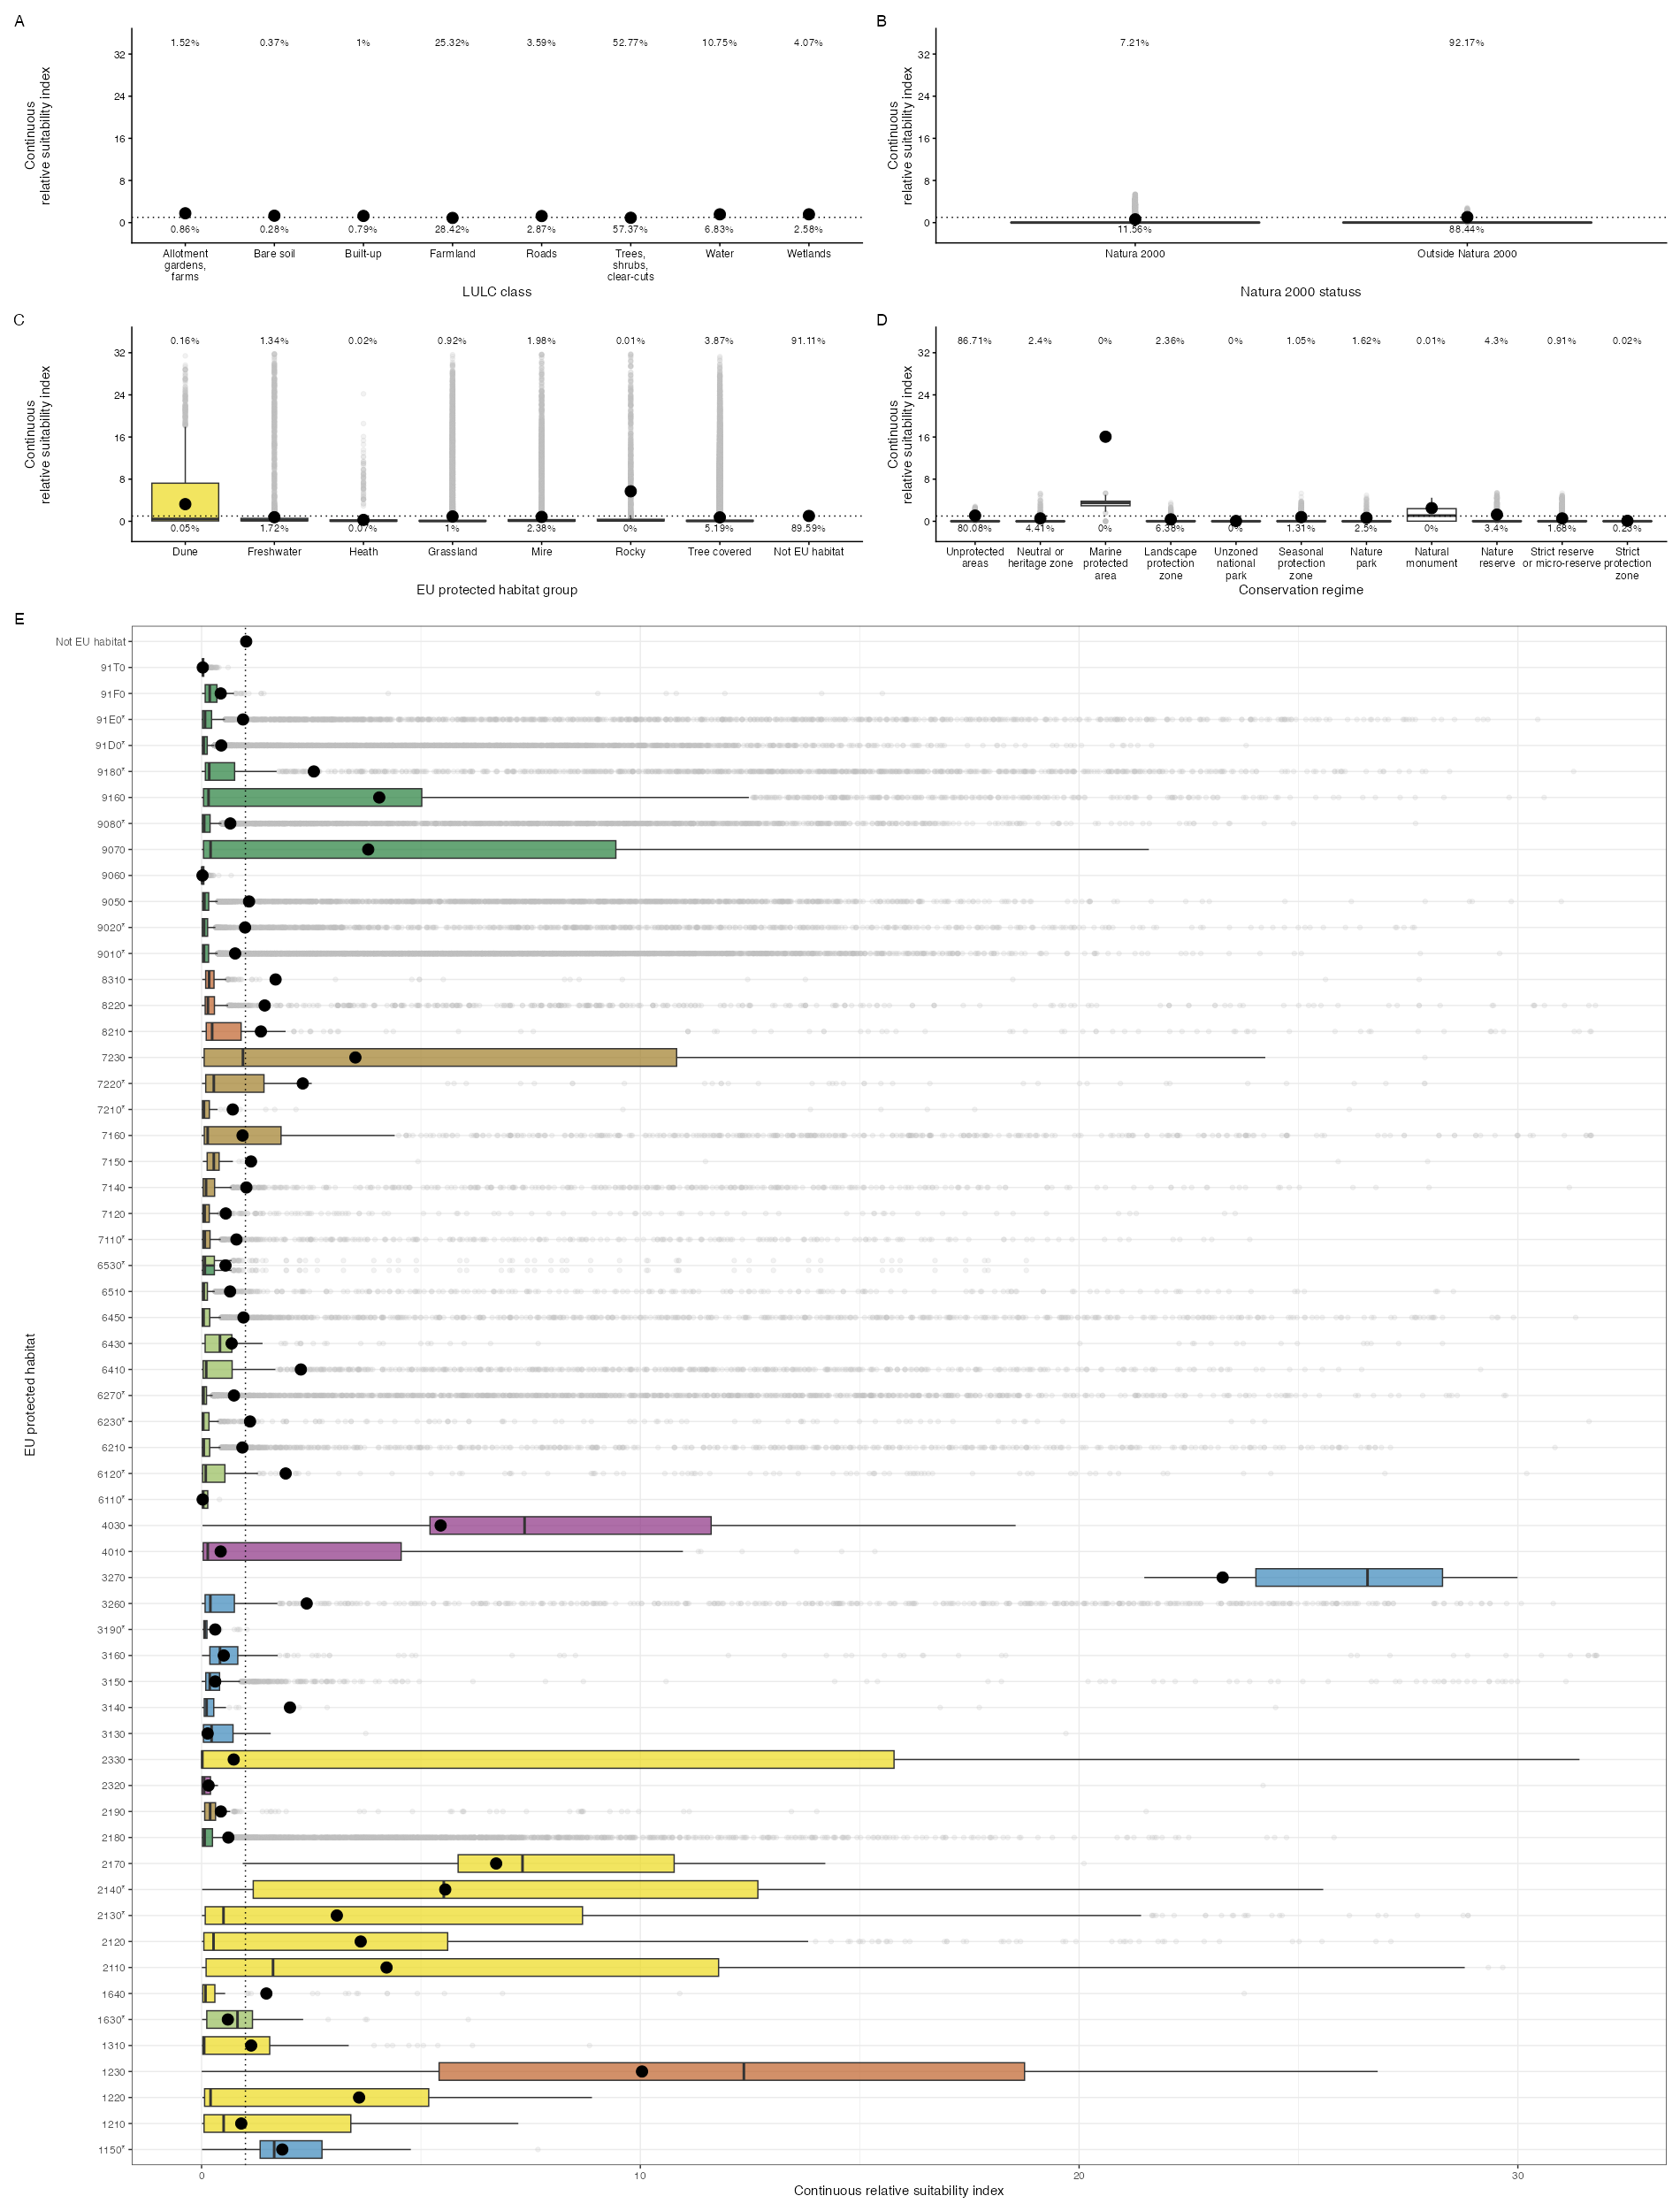
\includegraphics[width=1\linewidth,height=0.70\textheight,keepaspectratio]{results/HYLORIv4b1_2025/PicAssoc_HYLORI.png}

\par\small\textit{Associations between predicted suitability and: (A) land use land cover classes, (B) Natura 2000 status, (C) stratified EU protected habitat classes, (D) conservation regime, and (E) EU protected habitats. The y-axis show continuous relative suitability index (derivative of Manly's index of preference). Colours in (C) and (E) correspond to stratified EU protected habitat classes. For classifications composed of multiple individual polygons, polygon-level indices were additionally calculated to show within-category variation. The figures therefore combine category-level estimates (points) with the distributions of polygon-level values (boxplots, where applicable). Labels above and below the panels report, respectively, the percentage of total predicted suitability and the percentage of mapped area represented by each category. **For a full resolution refer to repository: link or online document: link**}\normalsize
\end{center}

\section*{Conservation prioritization}\label{conservation-prioritization-13}
\addcontentsline{toc}{section}{Conservation prioritization}

\begin{center}
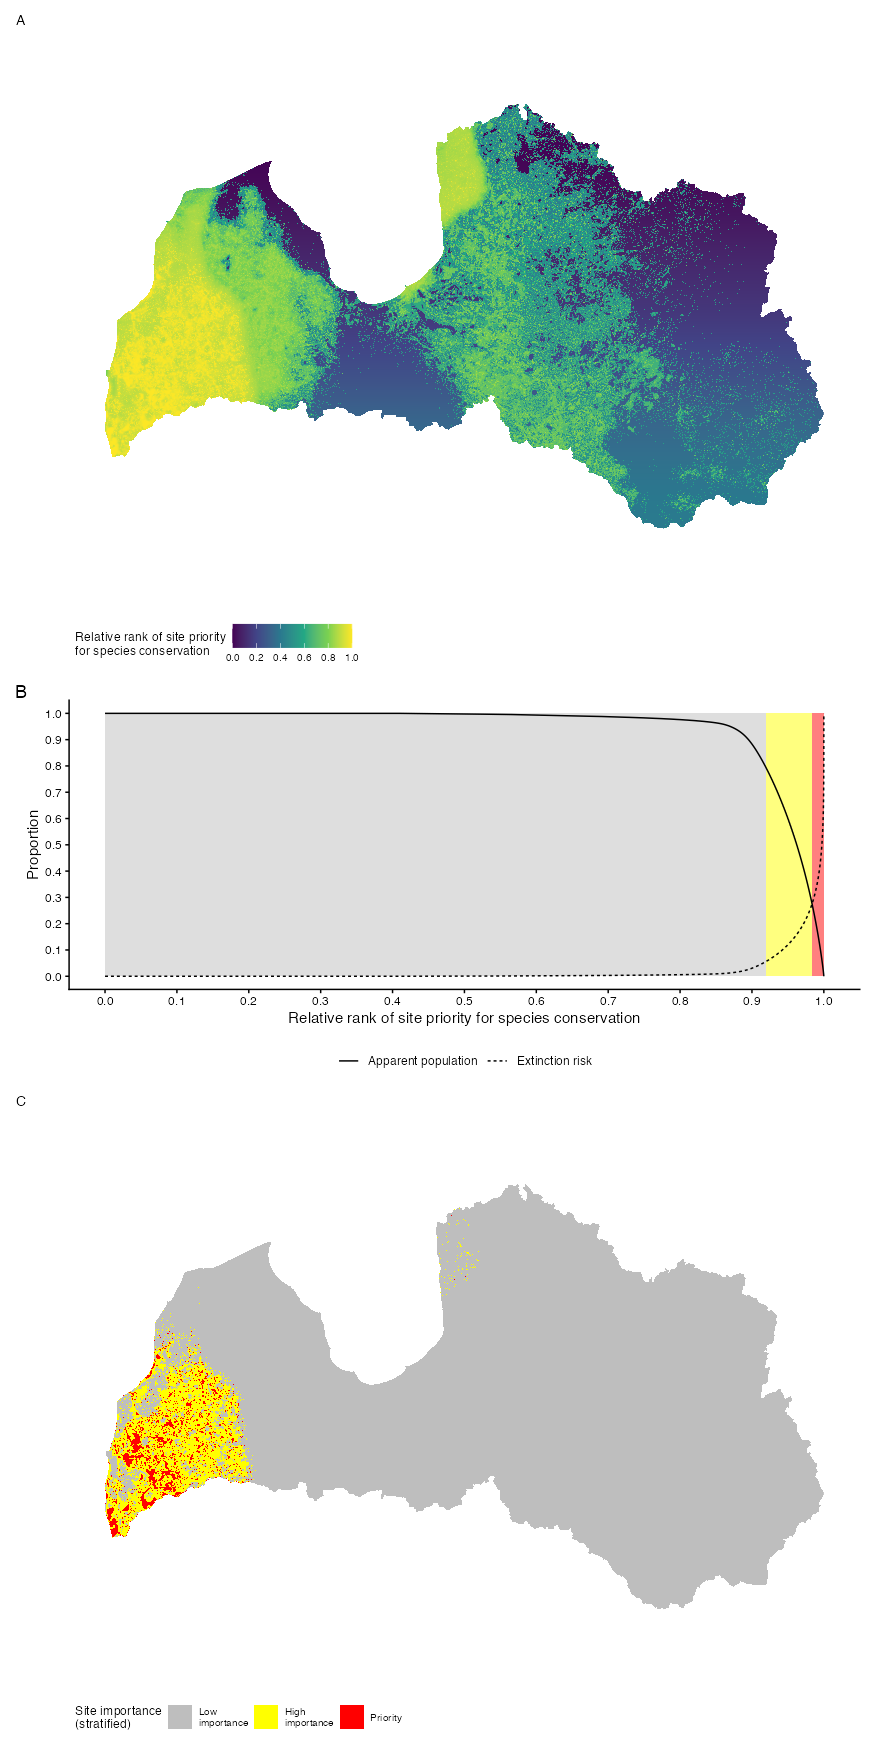
\includegraphics[width=0.85\linewidth,height=0.70\textheight,keepaspectratio]{results/HYLORIv4b1_2025/PicPrior_HYLORI.png}

\par\small\textit{Single-species conservation prioritization focusing on maximisation of core area protection (CAZMAX) while accounting for site connectivity: (A) relative site rank; (B) relationship between apparent-population and extinction-risk curves with a simplified classification which is spatially demonstrated in the bootom row; (C) spatial distribution of proposed classification of site prioritization results. **For a full resolution refer to repository: link or online document: link**}\normalsize
\end{center}

\chapter*{\texorpdfstring{\emph{Hyla orientalis} monitoring}{Hyla orientalis monitoring}}\label{hylorimonitoring}
\addcontentsline{toc}{chapter}{\emph{Hyla orientalis} monitoring}

\section*{Summary}\label{summary-14}
\addcontentsline{toc}{section}{Summary}

\subsection*{Model description}\label{model-description-14}
\addcontentsline{toc}{subsection}{Model description}

Occurrence and background data were divided into model-training with four block spatial cross-validation data and an independent test set. Sampling-bias/background treatment: \textbf{Phenology Weighted Target Group}. Accumulated LULC change within the 1-ha analysis cell was not evaluated; accumulated LULC change within the home-range radius around the analysis cell was not evaluated.

The final data set contained \textbf{99} presence records: \textbf{74} for training with four spatial block cross-validation and \textbf{25} for independent testing. Training background contained \textbf{29899} locations, with \textbf{10101} additional independent-test background locations.

\subsection*{Expert assessment scores}\label{expert-assessment-scores-14}
\addcontentsline{toc}{subsection}{Expert assessment scores}

\begin{itemize}
\tightlist
\item
  \textbf{Marginal responses and variable importance score:} 4 (good ecological interpretability)
\item
  \textbf{Map score:} 1 (poor agreement with known distribution)
\item
  \textbf{Applicability score:} 1 (very limited applicability)
\end{itemize}

\textbf{Šo sadaļu aizpildām manuāli no ekspertu aptaujām}

\subsection*{Statistical evaluation}\label{statistical-evaluation-14}
\addcontentsline{toc}{subsection}{Statistical evaluation}

The final model had a training TSS of \textbf{0.401}, with a training-derived cloglog threshold of \textbf{0.378}. Combined training AUC was \textbf{0.958} and combined test AUC was \textbf{0.906}.

\subsubsection*{Spatial cross-validation}\label{spatial-cross-validation-14}
\addcontentsline{toc}{subsubsection}{Spatial cross-validation}

\begin{itemize}
\tightlist
\item
  \textbf{AUC:} 0.8681 ± 0.1045; null models: 0.6798 ± 0.0383; z = 4.9189, p \textless{} 0.001
\item
  \textbf{CBI:} 0.6982 ± 0.1959; null models: 0.1238 ± 0.1164; z = 4.9337, p \textless{} 0.001
\item
  \textbf{OR10:} 0.1491 ± 0.0814; null models: 0.0208 ± 0.0347; z = 3.6925, p = 1
\item
  \textbf{ORmin:} 0.0687 ± 0.0701; null models: 0.0089 ± 0.0231; z = 2.5876, p = 0.995
\end{itemize}

\subsubsection*{Independent testing}\label{independent-testing-14}
\addcontentsline{toc}{subsubsection}{Independent testing}

\begin{itemize}
\tightlist
\item
  \textbf{TSS:} 0.465; \textbf{sensitivity:} 0.56; \textbf{specificity:} 0.905
\item
  \textbf{AUC:} 0.885; null models: 0.5136 ± 0.1764; z = 2.1077, p = 0.018
\item
  \textbf{CBI:} 0.523; null models: -0.0755 ± 0.5631; z = 1.0629, p = 0.144
\item
  \textbf{OR10:} 0.56; null models: 0.1628 ± 0.1671; z = 2.3765, p = 0.991
\item
  \textbf{ORmin:} 0.04; null models: 0.0264 ± 0.0602; z = 0.2258, p = 0.589
\end{itemize}

\subsection*{Conservation prioritisation summary}\label{conservation-prioritisation-summary-14}
\addcontentsline{toc}{subsection}{Conservation prioritisation summary}

The primary priority area covers \textbf{1.5\%} of Latvia and contains \textbf{27.6\%} of the summed habitat suitability (apparent population proxy).

The broader high importance area covers \textbf{2.5\%} of Latvia and contains \textbf{37.8\%} of the summed habitat suitability.

For comparison, the area classified as suitable using the maximum training sensitivity plus specificity habitat-suitability threshold contains \textbf{37.8\%} of the summed continuous habitat suitability.

\subsection*{Version evolution}\label{version-evolution-14}
\addcontentsline{toc}{subsection}{Version evolution}

\textbf{Šo sadaļu aizpildām manuāli, izmntojot sagatavotās shēmas. Jāvienojas par to noformējumu}

\section*{Habitat suitability}\label{habitat-suitability-14}
\addcontentsline{toc}{section}{Habitat suitability}

\begin{center}
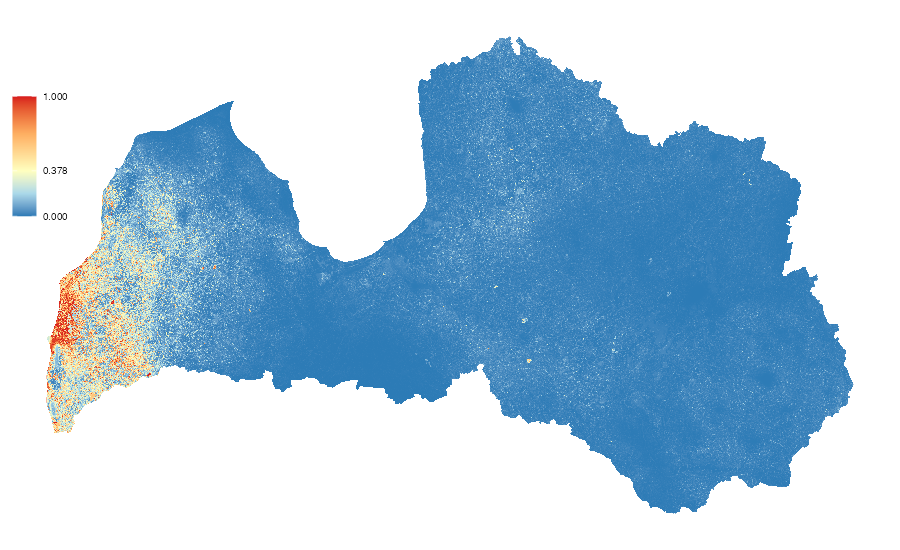
\includegraphics[width=1\linewidth,height=0.70\textheight,keepaspectratio]{results/HYLORImonitoring_v2b1/PicHSmap_HYLORImonitoring.png}

\par\small\textit{Predicted continuous habitat suitability across Latvia. The warmer the colour the higher is the predicted habitat suitability. Value in the middle of the legend correspond to the maximum training sensitivity plus specificity threshold. **For a full resolution refer to repository: link or online document: link**}\normalsize
\end{center}

\section*{Model thresholds}\label{model-thresholds-14}
\addcontentsline{toc}{section}{Model thresholds}

Threshold values and associated omission rates

\begin{center}
\resizebox{\linewidth}{!}{%

\begin{tabular}{lrrrrr}
\toprule
Threshold & Cloglog value & Fractional predicted area & Training omission rate & Test omission rate & P-values\\
\midrule
Minimum training presence & 0.0872276 & 0.2654672 & 0.0000000 & 0.0000987 & 0\\
Equal training sensitivity and specificity & 0.4443610 & 0.1003277 & 0.0945946 & 0.0013824 & 0\\
Maximum training sensitivity plus specificity & 0.3777838 & 0.1226339 & 0.0405405 & 0.0010862 & 0\\
Equal test sensitivity and specificity & 0.2178459 & 0.1854391 & 0.0270270 & 0.0003950 & 0\\
Maximum test sensitivity plus specificity & 0.1398980 & 0.2270417 & 0.0270270 & 0.0000987 & 0\\
\bottomrule
\end{tabular}
}
\end{center}

\section*{Variable importance}\label{variable-importance-14}
\addcontentsline{toc}{section}{Variable importance}

\begin{center}
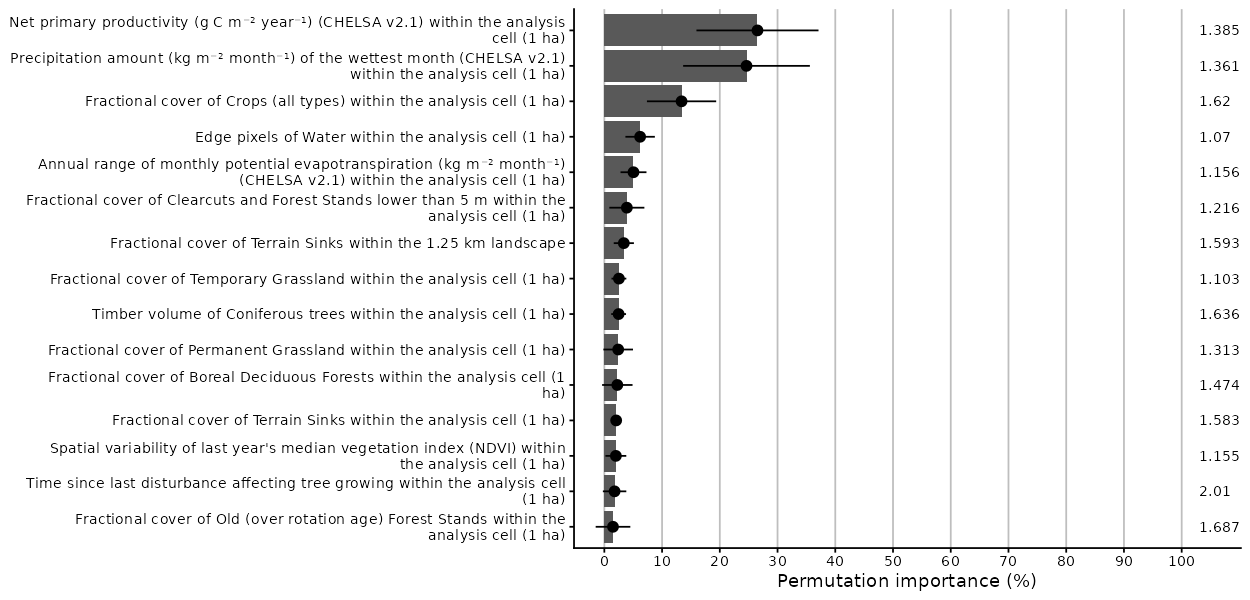
\includegraphics[width=1\linewidth,height=0.70\textheight,keepaspectratio]{results/HYLORImonitoring_v2b1/PicVarImpVIFs_HYLORImonitoring.png}

\par\small\textit{Permutation-importance (mean and standard deviation from 99 permutations, on the x-axis) of the ecogeographical variables (first y-axis, left side), and their variance inflation factor values (second y-axis, right side). **For a full resolution refer to repository: link or online document: link**}\normalsize
\end{center}

\section*{Marginal responses}\label{marginal-responses-14}
\addcontentsline{toc}{section}{Marginal responses}

\begin{center}
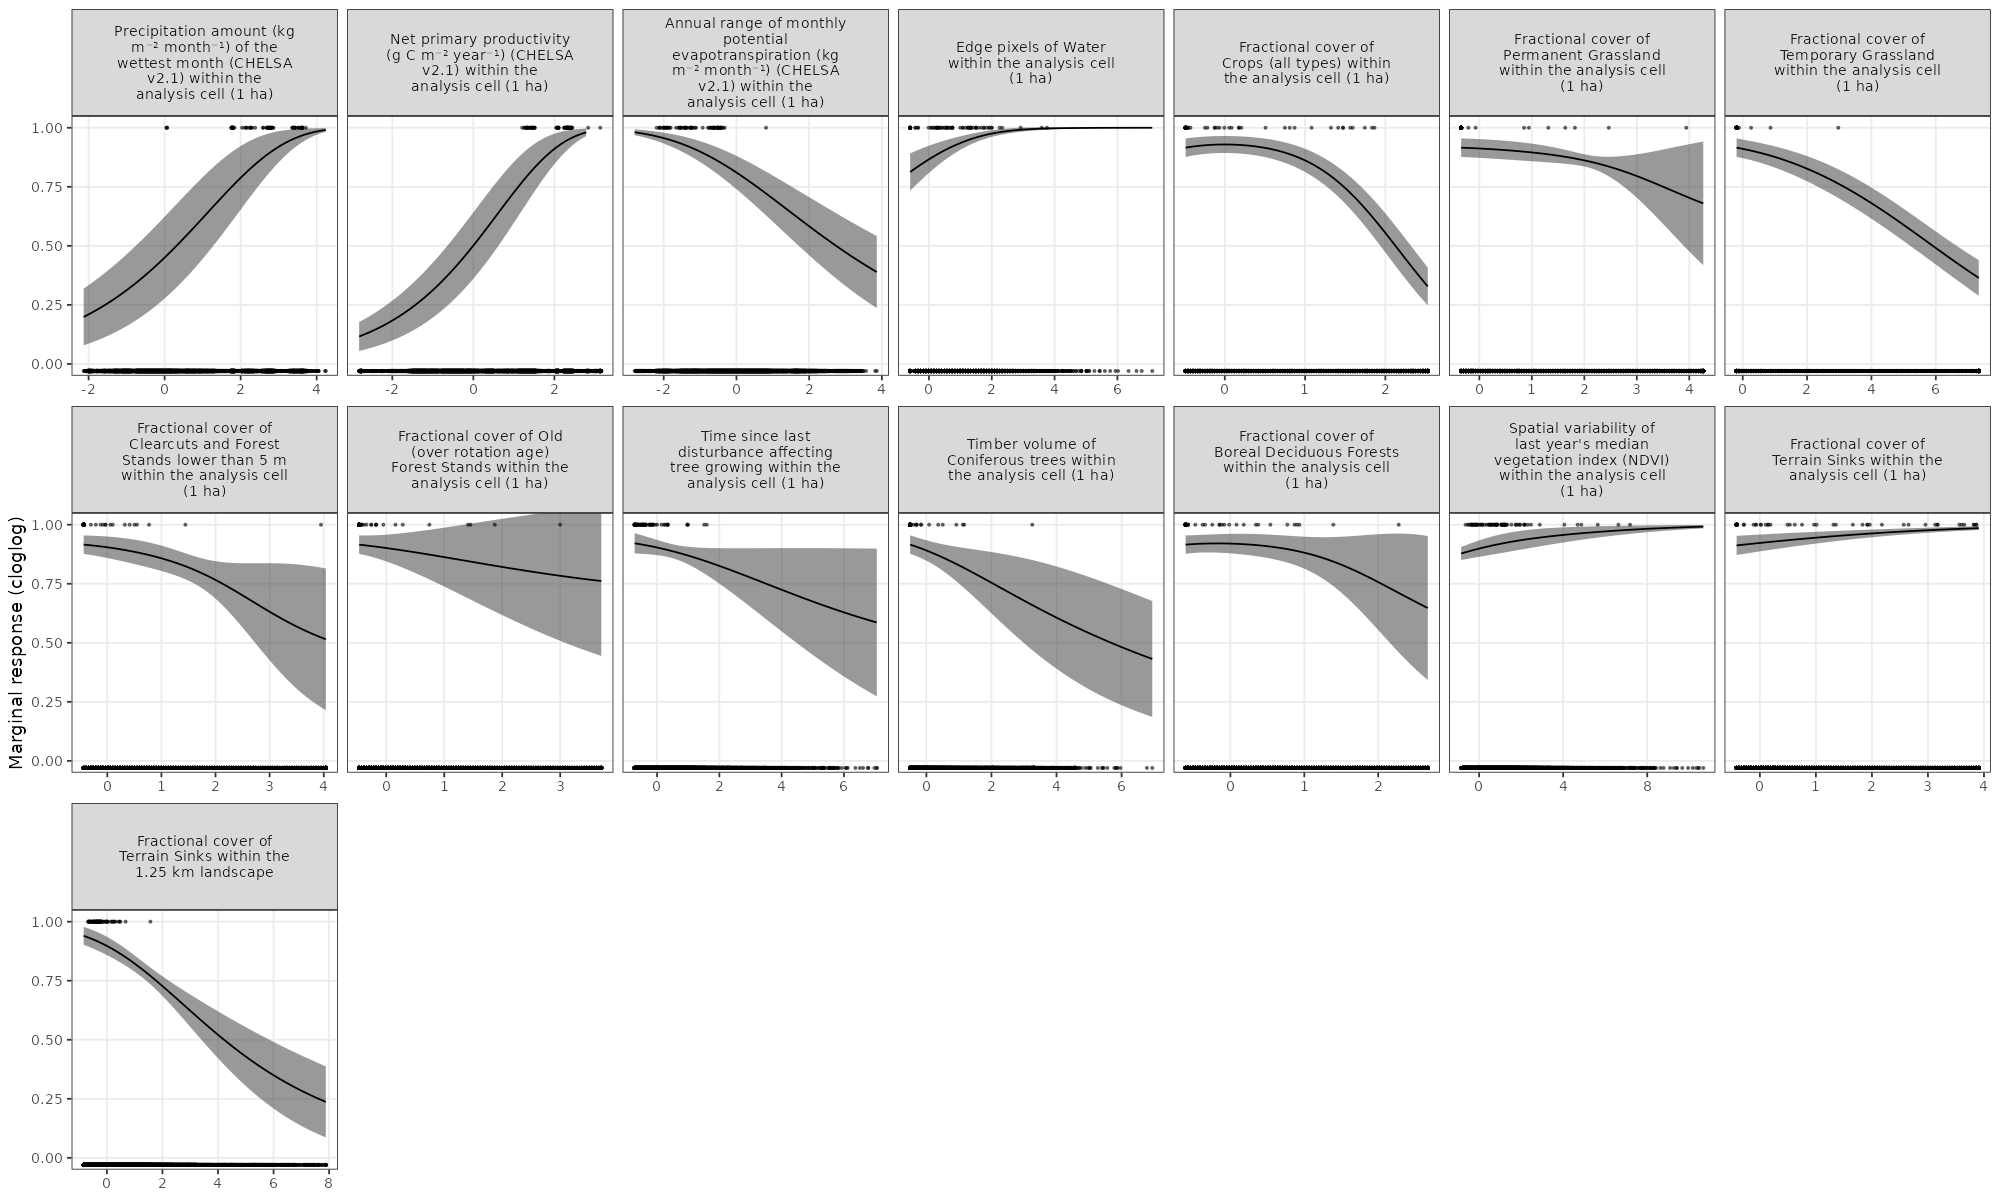
\includegraphics[width=1\linewidth,height=0.70\textheight,keepaspectratio]{results/HYLORImonitoring_v2b1/PicMargResp_HYLORImonitoring.png}

\par\small\textit{Marginalised for arithmetic mean response curves illustrating the effect of each ecogeographical variable on the habitat suitability when all the other variables have their arithmetic mean values. The y-axis shows the predicted habitat suitability (cloglog-transformed), while the x-axis shows the standardised (centred and scaled) value of the ecogeographical variable. Dots at a value of 1 on the y-axis illustrate presence locations in the environment (on the x-axis), while dots at a value of 0 illustrate background locations used in modelling.  **For a full resolution refer to repository: link or online document: link**}\normalsize
\end{center}

\section*{Habitat and conservation associations}\label{habitat-and-conservation-associations-14}
\addcontentsline{toc}{section}{Habitat and conservation associations}

\begin{center}
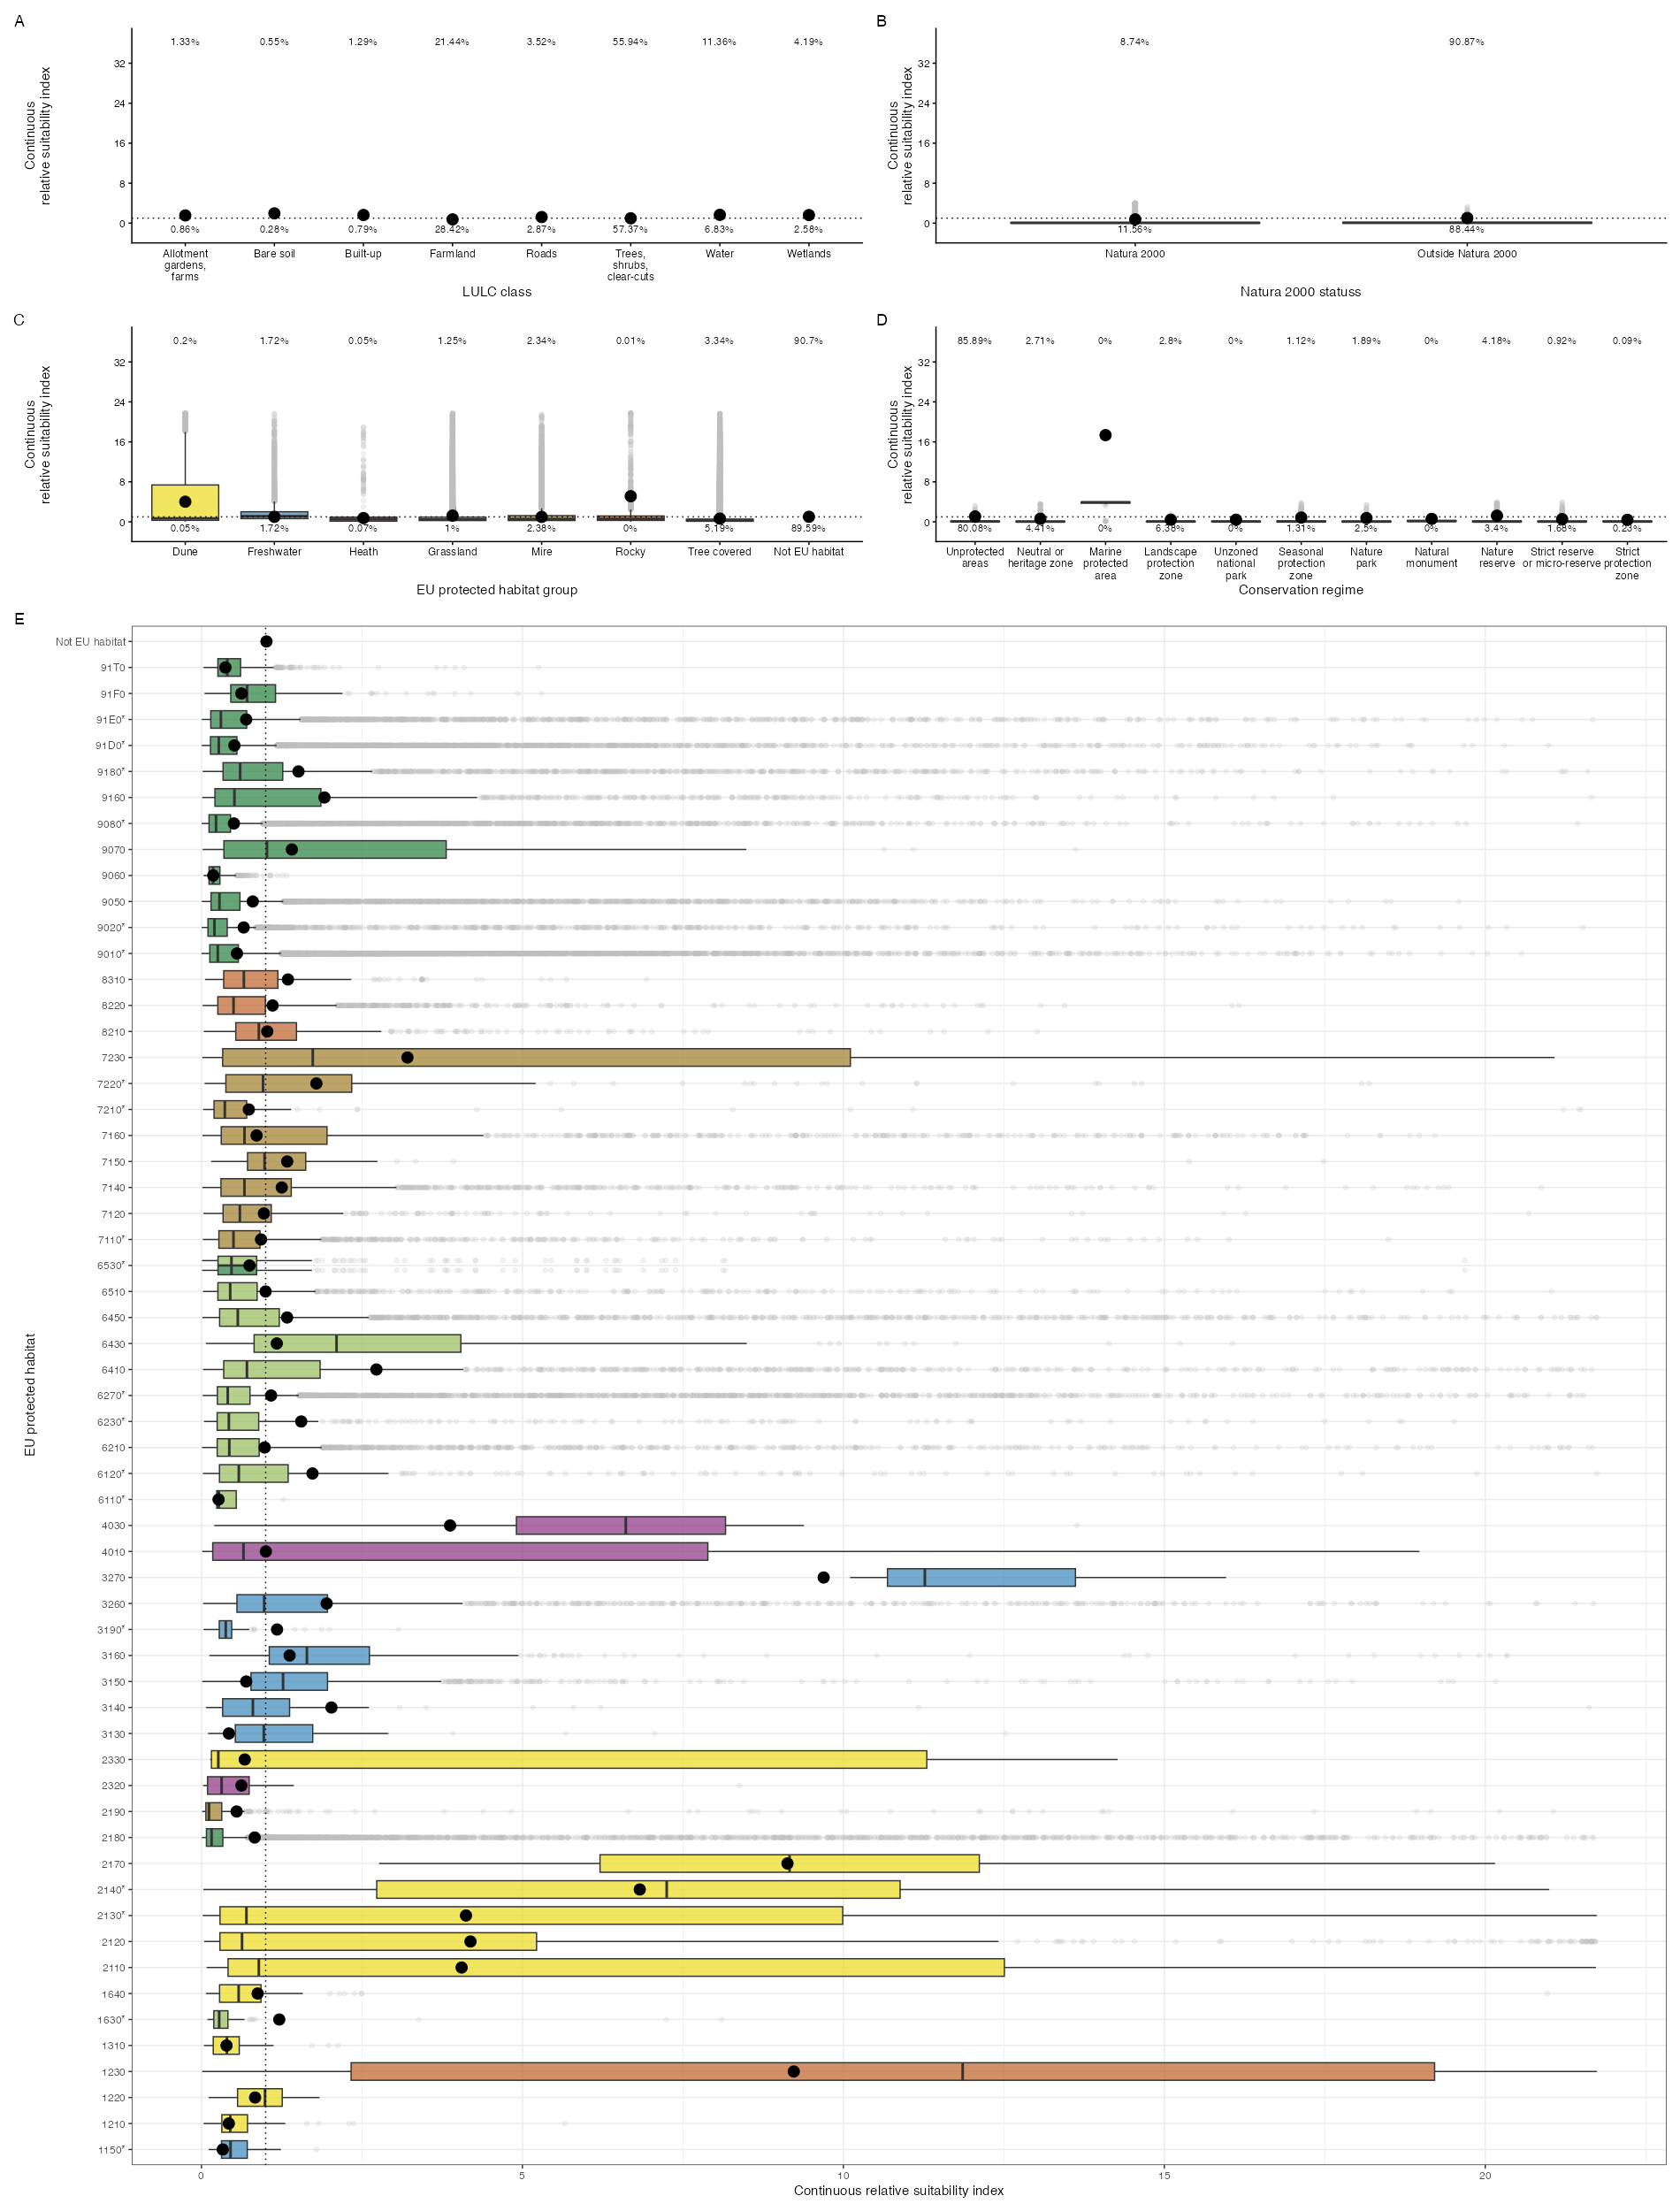
\includegraphics[width=1\linewidth,height=0.70\textheight,keepaspectratio]{results/HYLORImonitoring_v2b1/PicAssoc_HYLORImonitoring.png}

\par\small\textit{Associations between predicted suitability and: (A) land use land cover classes, (B) Natura 2000 status, (C) stratified EU protected habitat classes, (D) conservation regime, and (E) EU protected habitats. The y-axis show continuous relative suitability index (derivative of Manly's index of preference). Colours in (C) and (E) correspond to stratified EU protected habitat classes. For classifications composed of multiple individual polygons, polygon-level indices were additionally calculated to show within-category variation. The figures therefore combine category-level estimates (points) with the distributions of polygon-level values (boxplots, where applicable). Labels above and below the panels report, respectively, the percentage of total predicted suitability and the percentage of mapped area represented by each category. **For a full resolution refer to repository: link or online document: link**}\normalsize
\end{center}

\section*{Conservation prioritization}\label{conservation-prioritization-14}
\addcontentsline{toc}{section}{Conservation prioritization}

\begin{center}
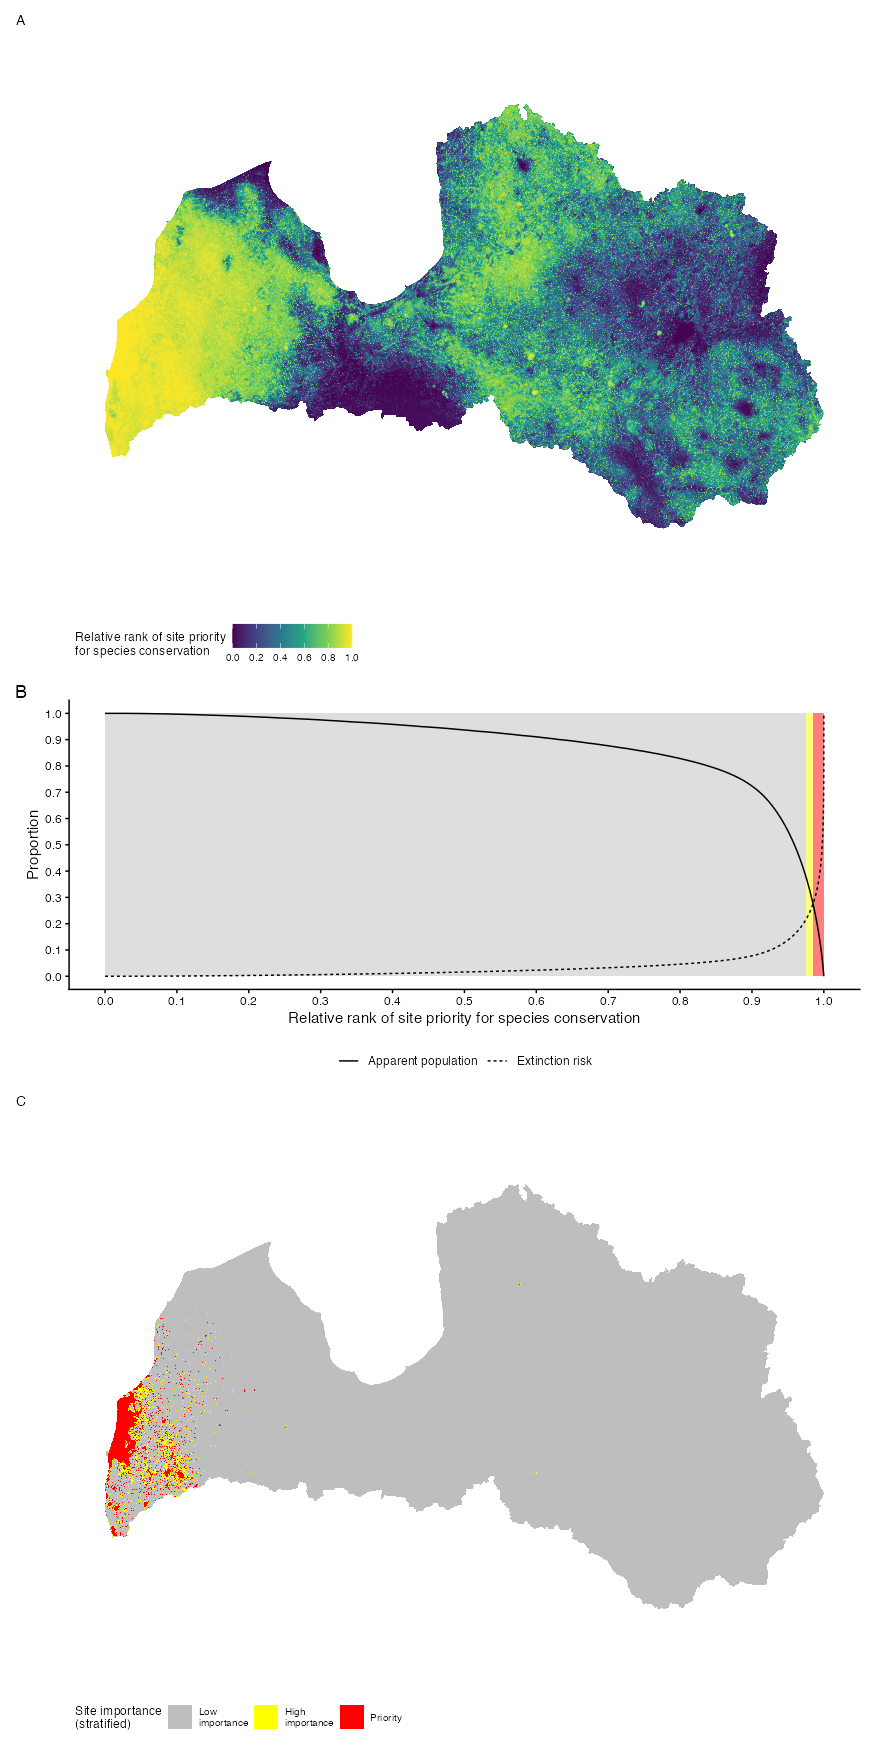
\includegraphics[width=0.85\linewidth,height=0.70\textheight,keepaspectratio]{results/HYLORImonitoring_v2b1/PicPrior_HYLORImonitoring.png}

\par\small\textit{Single-species conservation prioritization focusing on maximisation of core area protection (CAZMAX) while accounting for site connectivity: (A) relative site rank; (B) relationship between apparent-population and extinction-risk curves with a simplified classification which is spatially demonstrated in the bootom row; (C) spatial distribution of proposed classification of site prioritization results. **For a full resolution refer to repository: link or online document: link**}\normalsize
\end{center}

\chapter*{\texorpdfstring{\emph{Rana temporaria}}{Rana temporaria}}\label{rantem}
\addcontentsline{toc}{chapter}{\emph{Rana temporaria}}

\section*{Summary}\label{summary-15}
\addcontentsline{toc}{section}{Summary}

\subsection*{Model description}\label{model-description-15}
\addcontentsline{toc}{subsection}{Model description}

Occurrence and background data were divided into model-training with four block spatial cross-validation data and an independent test set. Sampling-bias/background treatment: \textbf{Phenology Weighted Target Group}. Accumulated LULC change within the 1-ha analysis cell was not evaluated; accumulated LULC change within the home-range radius around the analysis cell was not evaluated.

The final data set contained \textbf{370} presence records: \textbf{278} for training with four spatial block cross-validation and \textbf{92} for independent testing. Training background contained \textbf{30060} locations, with \textbf{9940} additional independent-test background locations.

\subsection*{Expert assessment scores}\label{expert-assessment-scores-15}
\addcontentsline{toc}{subsection}{Expert assessment scores}

\begin{itemize}
\tightlist
\item
  \textbf{Marginal responses and variable importance score:} 3 (moderate ecological interpretability)
\item
  \textbf{Map score:} 3 (moderate agreement with known distribution)
\item
  \textbf{Applicability score:} 2 (limited applicability)
\end{itemize}

\textbf{Šo sadaļu aizpildām manuāli no ekspertu aptaujām}

\subsection*{Statistical evaluation}\label{statistical-evaluation-15}
\addcontentsline{toc}{subsection}{Statistical evaluation}

The final model had a training TSS of \textbf{0.401}, with a training-derived cloglog threshold of \textbf{0.512}. Combined training AUC was \textbf{0.753} and combined test AUC was \textbf{0.67}.

\subsubsection*{Spatial cross-validation}\label{spatial-cross-validation-15}
\addcontentsline{toc}{subsubsection}{Spatial cross-validation}

\begin{itemize}
\tightlist
\item
  \textbf{AUC:} 0.689 ± 0.0395; null models: 0.5246 ± 0.0242; z = 6.7886, p \textless{} 0.001
\item
  \textbf{CBI:} 0.8465 ± 0.0962; null models: 0.179 ± 0.1705; z = 3.9141, p \textless{} 0.001
\item
  \textbf{OR10:} 0.1547 ± 0.018; null models: 0.1391 ± 0.051; z = 0.3059, p = 0.62
\item
  \textbf{ORmin:} 0.0036 ± 0.0072; null models: 0.0121 ± 0.0313; z = -0.2708, p = 0.393
\end{itemize}

\subsubsection*{Independent testing}\label{independent-testing-15}
\addcontentsline{toc}{subsubsection}{Independent testing}

\begin{itemize}
\tightlist
\item
  \textbf{TSS:} 0.254; \textbf{sensitivity:} 0.565; \textbf{specificity:} 0.689
\item
  \textbf{AUC:} 0.655; null models: 0.5012 ± 0.0777; z = 1.9771, p = 0.024
\item
  \textbf{CBI:} 0.755; null models: -0.0036 ± 0.5202; z = 1.4583, p = 0.072
\item
  \textbf{OR10:} 0.239; null models: 0.1346 ± 0.0762; z = 1.3728, p = 0.915
\item
  \textbf{ORmin:} 0.011; null models: 0.0065 ± 0.0153; z = 0.2843, p = 0.612
\end{itemize}

\subsection*{Conservation prioritisation summary}\label{conservation-prioritisation-summary-15}
\addcontentsline{toc}{subsection}{Conservation prioritisation summary}

The primary priority area covers \textbf{13.7\%} of Latvia and contains \textbf{27.6\%} of the summed habitat suitability (apparent population proxy).

The broader high importance area covers \textbf{30\%} of Latvia and contains \textbf{50.3\%} of the summed habitat suitability.

For comparison, the area classified as suitable using the maximum training sensitivity plus specificity habitat-suitability threshold contains \textbf{50.3\%} of the summed continuous habitat suitability.

\subsection*{Version evolution}\label{version-evolution-15}
\addcontentsline{toc}{subsection}{Version evolution}

\textbf{Šo sadaļu aizpildām manuāli, izmntojot sagatavotās shēmas. Jāvienojas par to noformējumu}

\section*{Habitat suitability}\label{habitat-suitability-15}
\addcontentsline{toc}{section}{Habitat suitability}

\begin{center}
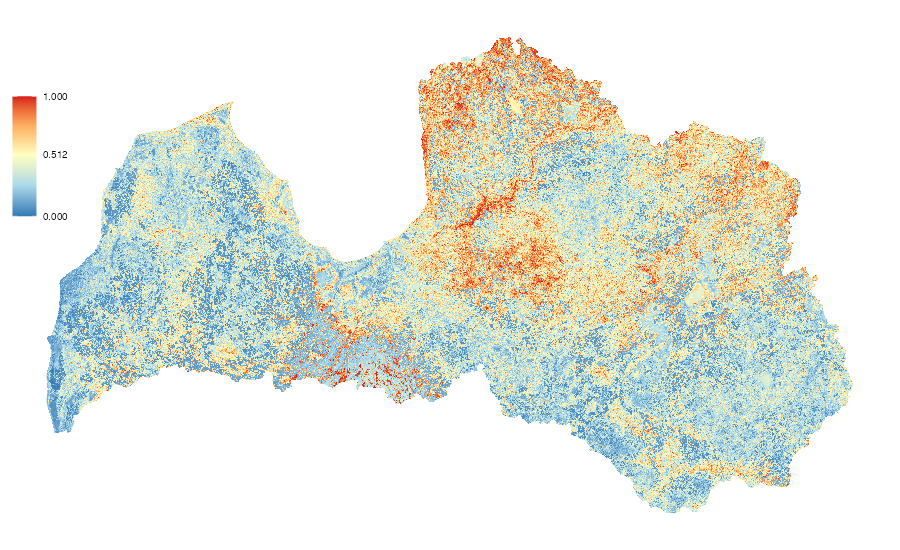
\includegraphics[width=1\linewidth,height=0.70\textheight,keepaspectratio]{results/RANTEMv5b1NM/PicHSmap_RANTEM.png}

\par\small\textit{Predicted continuous habitat suitability across Latvia. The warmer the colour the higher is the predicted habitat suitability. Value in the middle of the legend correspond to the maximum training sensitivity plus specificity threshold. **For a full resolution refer to repository: link or online document: link**}\normalsize
\end{center}

\section*{Model thresholds}\label{model-thresholds-15}
\addcontentsline{toc}{section}{Model thresholds}

Threshold values and associated omission rates

\begin{center}
\resizebox{\linewidth}{!}{%

\begin{tabular}{lrrrrr}
\toprule
Threshold & Cloglog value & Fractional predicted area & Training omission rate & Test omission rate & P-values\\
\midrule
Minimum training presence & 0.1411613 & 0.8974817 & 0.0000000 & 0.0000992 & 0\\
Equal training sensitivity and specificity & 0.5254056 & 0.3165444 & 0.3165468 & 0.0039671 & 0\\
Maximum training sensitivity plus specificity & 0.5123521 & 0.3360764 & 0.2841727 & 0.0039671 & 0\\
Equal test sensitivity and specificity & 0.4600672 & 0.4171459 & 0.2374101 & 0.0034712 & 0\\
Maximum test sensitivity plus specificity & 0.6473170 & 0.1823650 & 0.4676259 & 0.0049588 & 0\\
\bottomrule
\end{tabular}
}
\end{center}

\section*{Variable importance}\label{variable-importance-15}
\addcontentsline{toc}{section}{Variable importance}

\begin{center}
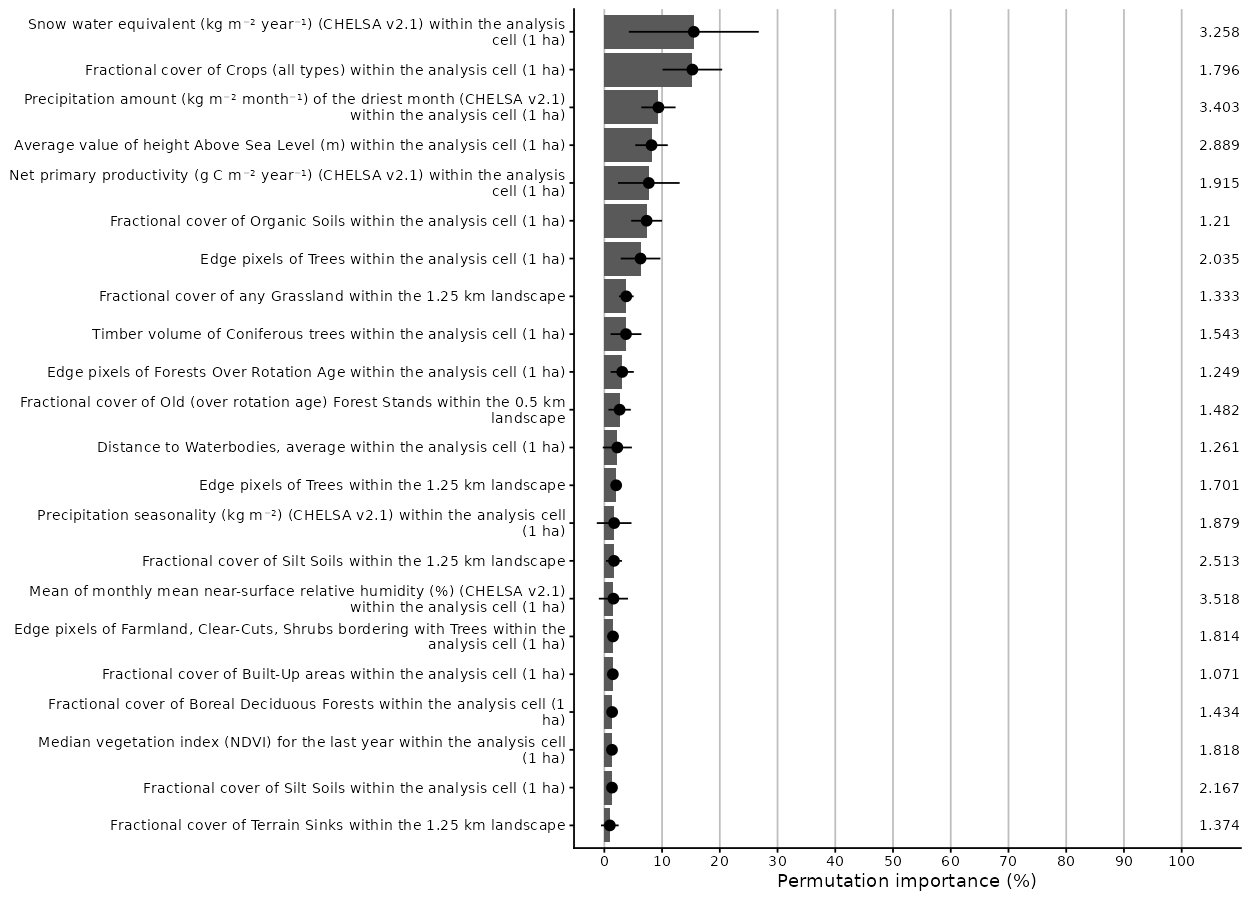
\includegraphics[width=1\linewidth,height=0.70\textheight,keepaspectratio]{results/RANTEMv5b1NM/PicVarImpVIFs_RANTEM.png}

\par\small\textit{Permutation-importance (mean and standard deviation from 99 permutations, on the x-axis) of the ecogeographical variables (first y-axis, left side), and their variance inflation factor values (second y-axis, right side). **For a full resolution refer to repository: link or online document: link**}\normalsize
\end{center}

\section*{Marginal responses}\label{marginal-responses-15}
\addcontentsline{toc}{section}{Marginal responses}

\begin{center}
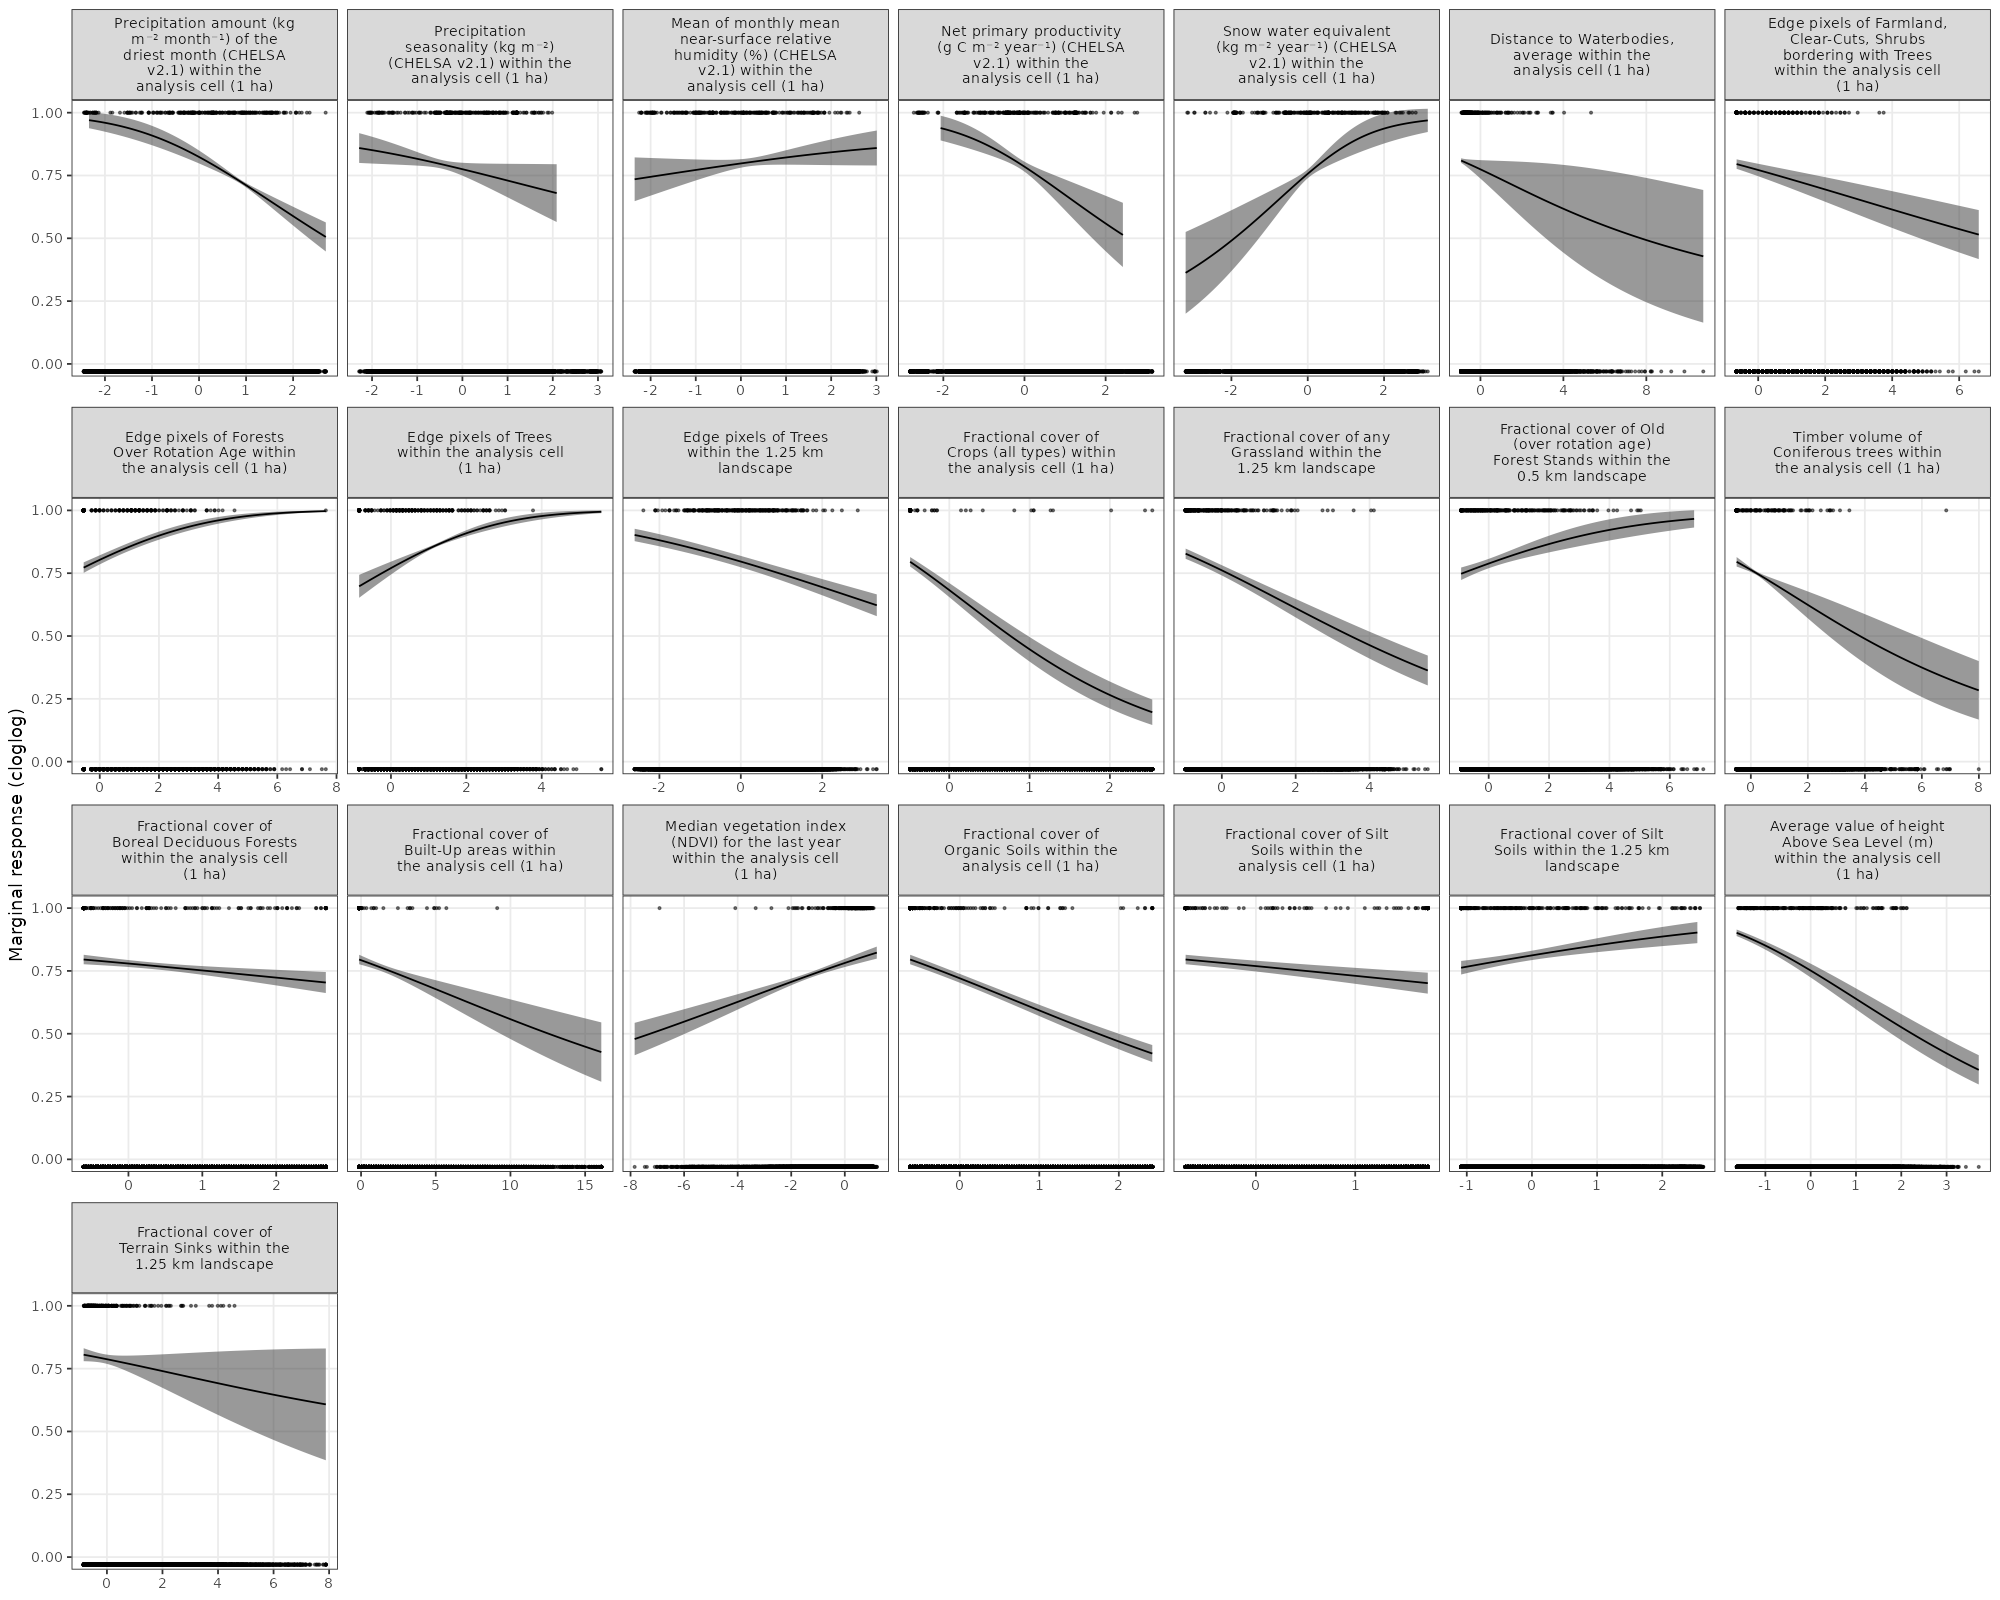
\includegraphics[width=1\linewidth,height=0.70\textheight,keepaspectratio]{results/RANTEMv5b1NM/PicMargResp_RANTEM.png}

\par\small\textit{Marginalised for arithmetic mean response curves illustrating the effect of each ecogeographical variable on the habitat suitability when all the other variables have their arithmetic mean values. The y-axis shows the predicted habitat suitability (cloglog-transformed), while the x-axis shows the standardised (centred and scaled) value of the ecogeographical variable. Dots at a value of 1 on the y-axis illustrate presence locations in the environment (on the x-axis), while dots at a value of 0 illustrate background locations used in modelling.  **For a full resolution refer to repository: link or online document: link**}\normalsize
\end{center}

\section*{Habitat and conservation associations}\label{habitat-and-conservation-associations-15}
\addcontentsline{toc}{section}{Habitat and conservation associations}

\begin{center}
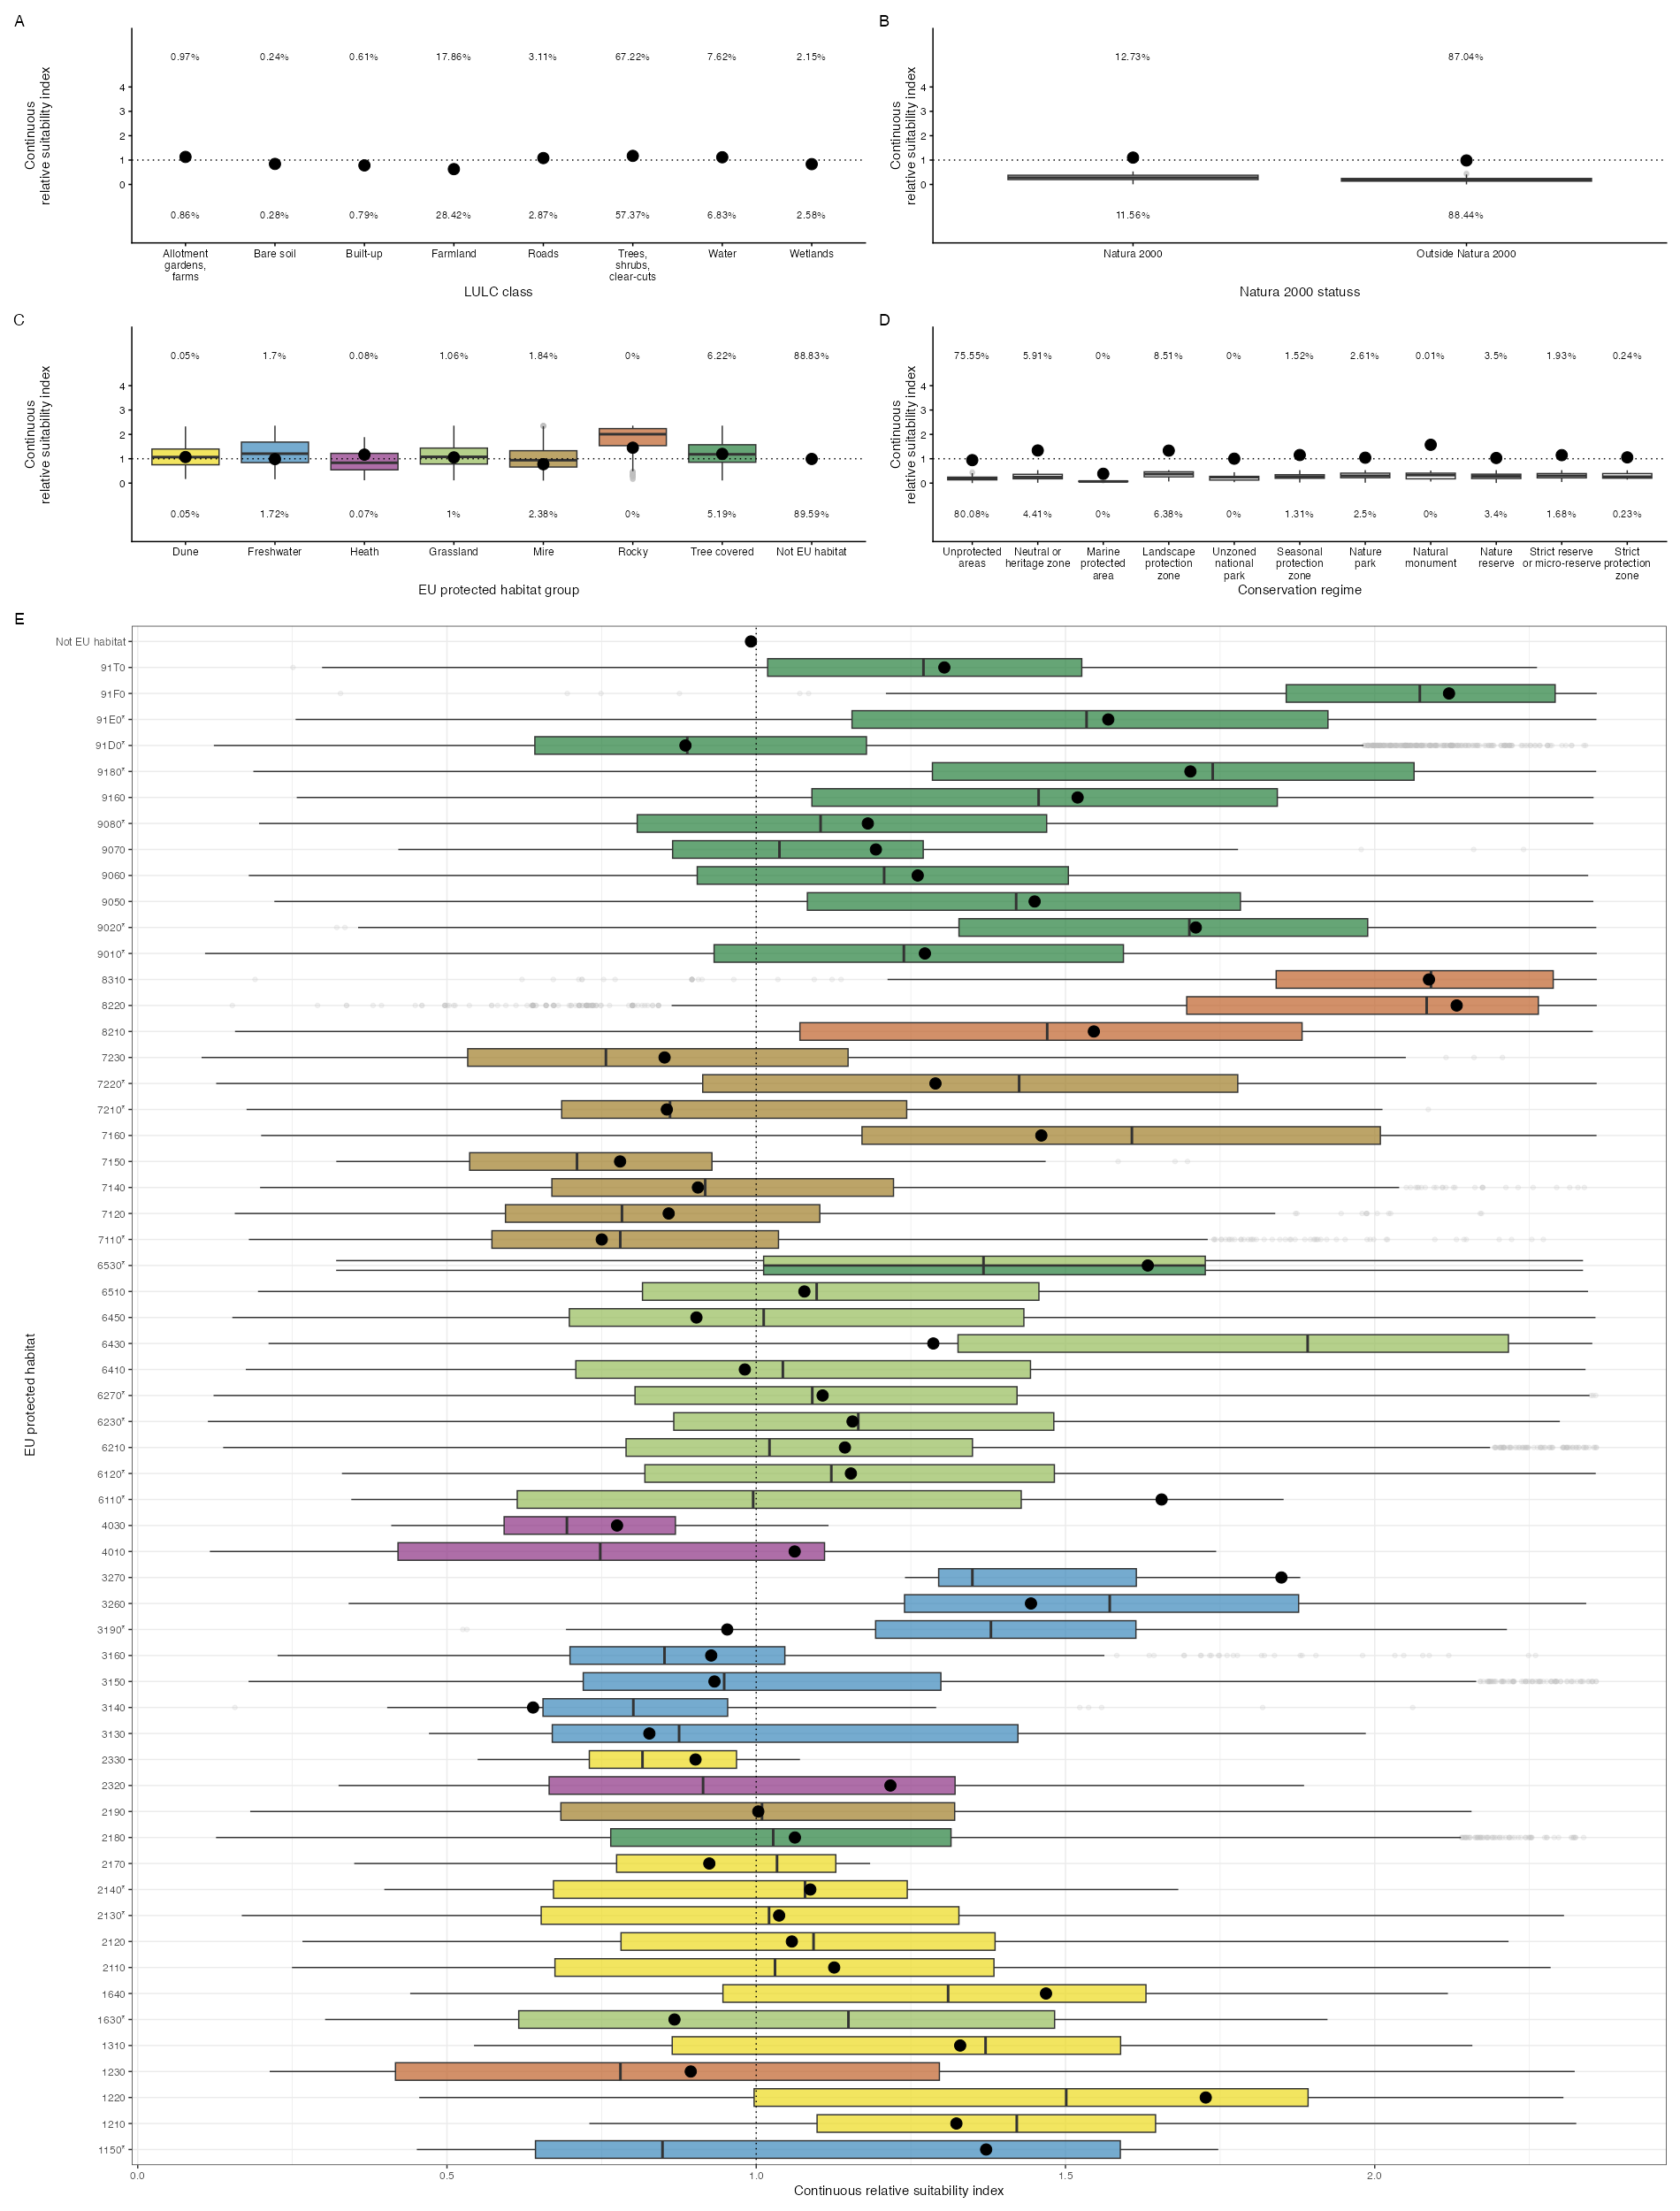
\includegraphics[width=1\linewidth,height=0.70\textheight,keepaspectratio]{results/RANTEMv5b1NM/PicAssoc_RANTEM.png}

\par\small\textit{Associations between predicted suitability and: (A) land use land cover classes, (B) Natura 2000 status, (C) stratified EU protected habitat classes, (D) conservation regime, and (E) EU protected habitats. The y-axis show continuous relative suitability index (derivative of Manly's index of preference). Colours in (C) and (E) correspond to stratified EU protected habitat classes. For classifications composed of multiple individual polygons, polygon-level indices were additionally calculated to show within-category variation. The figures therefore combine category-level estimates (points) with the distributions of polygon-level values (boxplots, where applicable). Labels above and below the panels report, respectively, the percentage of total predicted suitability and the percentage of mapped area represented by each category. **For a full resolution refer to repository: link or online document: link**}\normalsize
\end{center}

\section*{Conservation prioritization}\label{conservation-prioritization-15}
\addcontentsline{toc}{section}{Conservation prioritization}

\begin{center}
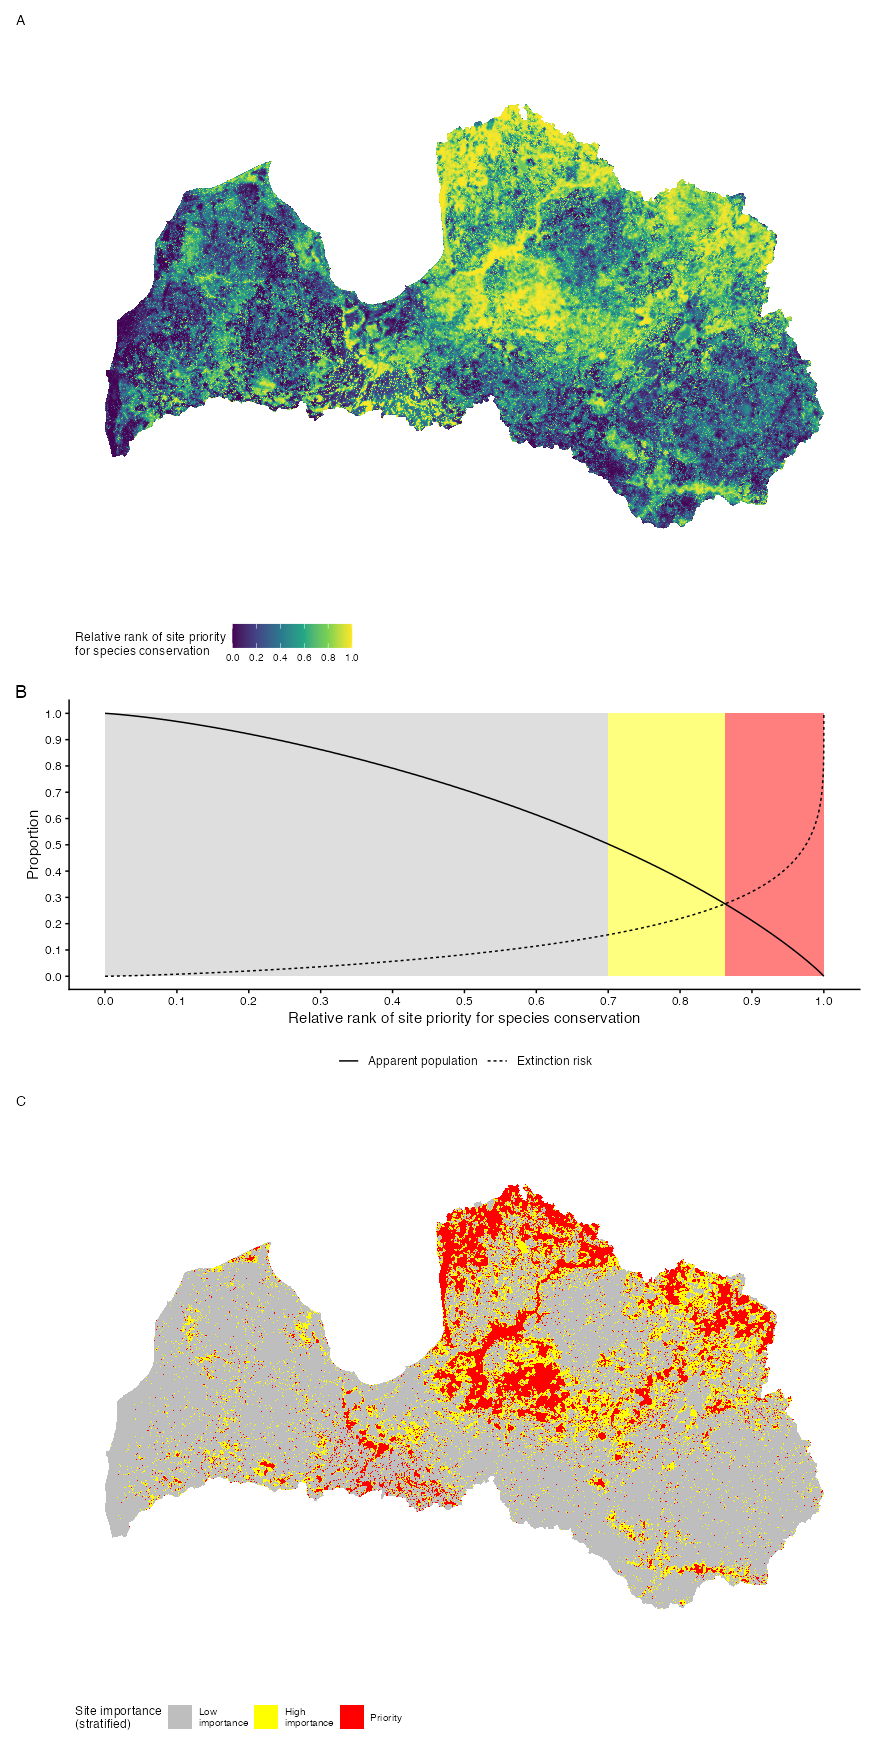
\includegraphics[width=0.85\linewidth,height=0.70\textheight,keepaspectratio]{results/RANTEMv5b1NM/PicPrior_RANTEM.png}

\par\small\textit{Single-species conservation prioritization focusing on maximisation of core area protection (CAZMAX) while accounting for site connectivity: (A) relative site rank; (B) relationship between apparent-population and extinction-risk curves with a simplified classification which is spatially demonstrated in the bootom row; (C) spatial distribution of proposed classification of site prioritization results. **For a full resolution refer to repository: link or online document: link**}\normalsize
\end{center}

\chapter*{\texorpdfstring{\emph{Rana temporaria} terrestrial}{Rana temporaria terrestrial}}\label{rantemterrestrial}
\addcontentsline{toc}{chapter}{\emph{Rana temporaria} terrestrial}

\section*{Summary}\label{summary-16}
\addcontentsline{toc}{section}{Summary}

\subsection*{Model description}\label{model-description-16}
\addcontentsline{toc}{subsection}{Model description}

Occurrence and background data were divided into model-training with four block spatial cross-validation data and an independent test set. Sampling-bias/background treatment: \textbf{Phenology Weighted Target Group}. Accumulated LULC change within the 1-ha analysis cell was not evaluated; accumulated LULC change within the home-range radius around the analysis cell was not evaluated.

The final data set contained \textbf{322} presence records: \textbf{242} for training with four spatial block cross-validation and \textbf{80} for independent testing. Training background contained \textbf{30065} locations, with \textbf{9935} additional independent-test background locations.

\subsection*{Expert assessment scores}\label{expert-assessment-scores-16}
\addcontentsline{toc}{subsection}{Expert assessment scores}

\begin{itemize}
\tightlist
\item
  \textbf{Marginal responses and variable importance score:} 2 (limited ecological interpretability)
\item
  \textbf{Map score:} 2 (limited agreement with known distribution)
\item
  \textbf{Applicability score:} 1 (very limited applicability)
\end{itemize}

\textbf{Šo sadaļu aizpildām manuāli no ekspertu aptaujām}

\subsection*{Statistical evaluation}\label{statistical-evaluation-16}
\addcontentsline{toc}{subsection}{Statistical evaluation}

The final model had a training TSS of \textbf{0.401}, with a training-derived cloglog threshold of \textbf{0.611}. Combined training AUC was \textbf{0.777} and combined test AUC was \textbf{0.67}.

\subsubsection*{Spatial cross-validation}\label{spatial-cross-validation-16}
\addcontentsline{toc}{subsubsection}{Spatial cross-validation}

\begin{itemize}
\tightlist
\item
  \textbf{AUC:} 0.6426 ± 0.0251; null models: 0.5152 ± 0.0265; z = 4.8079, p \textless{} 0.001
\item
  \textbf{CBI:} 0.6662 ± 0.1288; null models: 0.0897 ± 0.1431; z = 4.0281, p \textless{} 0.001
\item
  \textbf{OR10:} 0.2361 ± 0.162; null models: 0.111 ± 0.0602; z = 2.0798, p = 0.981
\item
  \textbf{ORmin:} 0.0249 ± 0.0319; null models: 0.0186 ± 0.0475; z = 0.1325, p = 0.553
\end{itemize}

\subsubsection*{Independent testing}\label{independent-testing-16}
\addcontentsline{toc}{subsubsection}{Independent testing}

\begin{itemize}
\tightlist
\item
  \textbf{TSS:} 0.14; \textbf{sensitivity:} 0.3; \textbf{specificity:} 0.84
\item
  \textbf{AUC:} 0.623; null models: 0.5063 ± 0.0679; z = 1.7248, p = 0.042
\item
  \textbf{CBI:} 0.559; null models: 0.0126 ± 0.4552; z = 1.2003, p = 0.115
\item
  \textbf{OR10:} 0.238; null models: 0.1568 ± 0.0683; z = 1.1817, p = 0.881
\item
  \textbf{ORmin:} 0; null models: 0.0099 ± 0.015; z = -0.6583, p = 0.255
\end{itemize}

\subsection*{Conservation prioritisation summary}\label{conservation-prioritisation-summary-16}
\addcontentsline{toc}{subsection}{Conservation prioritisation summary}

The primary priority area covers \textbf{13\%} of Latvia and contains \textbf{27.6\%} of the summed habitat suitability (apparent population proxy).

The broader high importance area covers \textbf{16.1\%} of Latvia and contains \textbf{32.6\%} of the summed habitat suitability.

For comparison, the area classified as suitable using the maximum training sensitivity plus specificity habitat-suitability threshold contains \textbf{32.5\%} of the summed continuous habitat suitability.

\subsection*{Version evolution}\label{version-evolution-16}
\addcontentsline{toc}{subsection}{Version evolution}

\textbf{Šo sadaļu aizpildām manuāli, izmntojot sagatavotās shēmas. Jāvienojas par to noformējumu}

\section*{Habitat suitability}\label{habitat-suitability-16}
\addcontentsline{toc}{section}{Habitat suitability}

\begin{center}
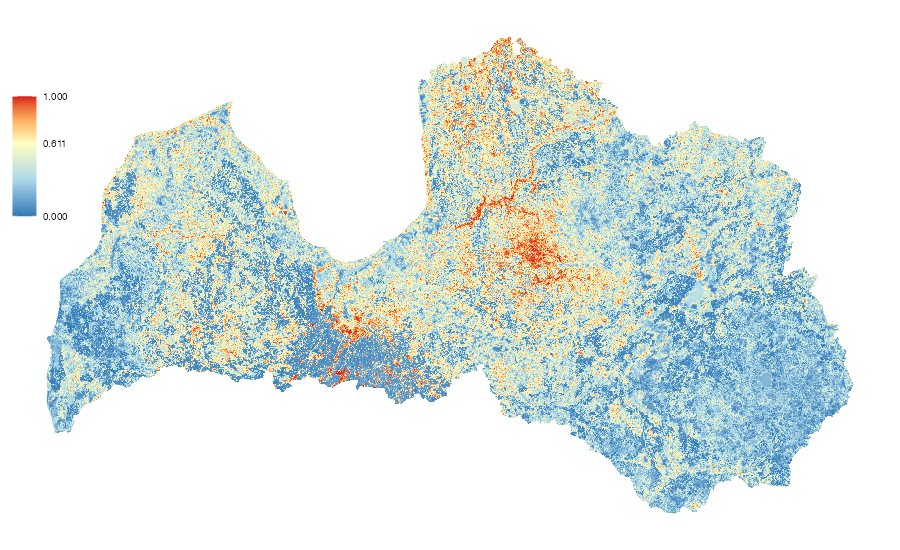
\includegraphics[width=1\linewidth,height=0.70\textheight,keepaspectratio]{results/RANTEMterrestrialv2b1celi/PicHSmap_RANTEMterrestrial.png}

\par\small\textit{Predicted continuous habitat suitability across Latvia. The warmer the colour the higher is the predicted habitat suitability. Value in the middle of the legend correspond to the maximum training sensitivity plus specificity threshold. **For a full resolution refer to repository: link or online document: link**}\normalsize
\end{center}

\section*{Model thresholds}\label{model-thresholds-16}
\addcontentsline{toc}{section}{Model thresholds}

Threshold values and associated omission rates

\begin{center}
\resizebox{\linewidth}{!}{%

\begin{tabular}{lrrrrr}
\toprule
Threshold & Cloglog value & Fractional predicted area & Training omission rate & Test omission rate & P-values\\
\midrule
Minimum training presence & 0.1140901 & 0.8791944 & 0.0000000 & 0.0000000 & 0\\
Equal training sensitivity and specificity & 0.5292742 & 0.3016662 & 0.3016529 & 0.0046775 & 0\\
Maximum training sensitivity plus specificity & 0.6109006 & 0.2166683 & 0.3719008 & 0.0055732 & 0\\
Equal test sensitivity and specificity & 0.4399037 & 0.4123025 & 0.1983471 & 0.0029857 & 0\\
Maximum test sensitivity plus specificity & 0.4307822 & 0.4255192 & 0.1859504 & 0.0025876 & 0\\
\bottomrule
\end{tabular}
}
\end{center}

\section*{Variable importance}\label{variable-importance-16}
\addcontentsline{toc}{section}{Variable importance}

\begin{center}
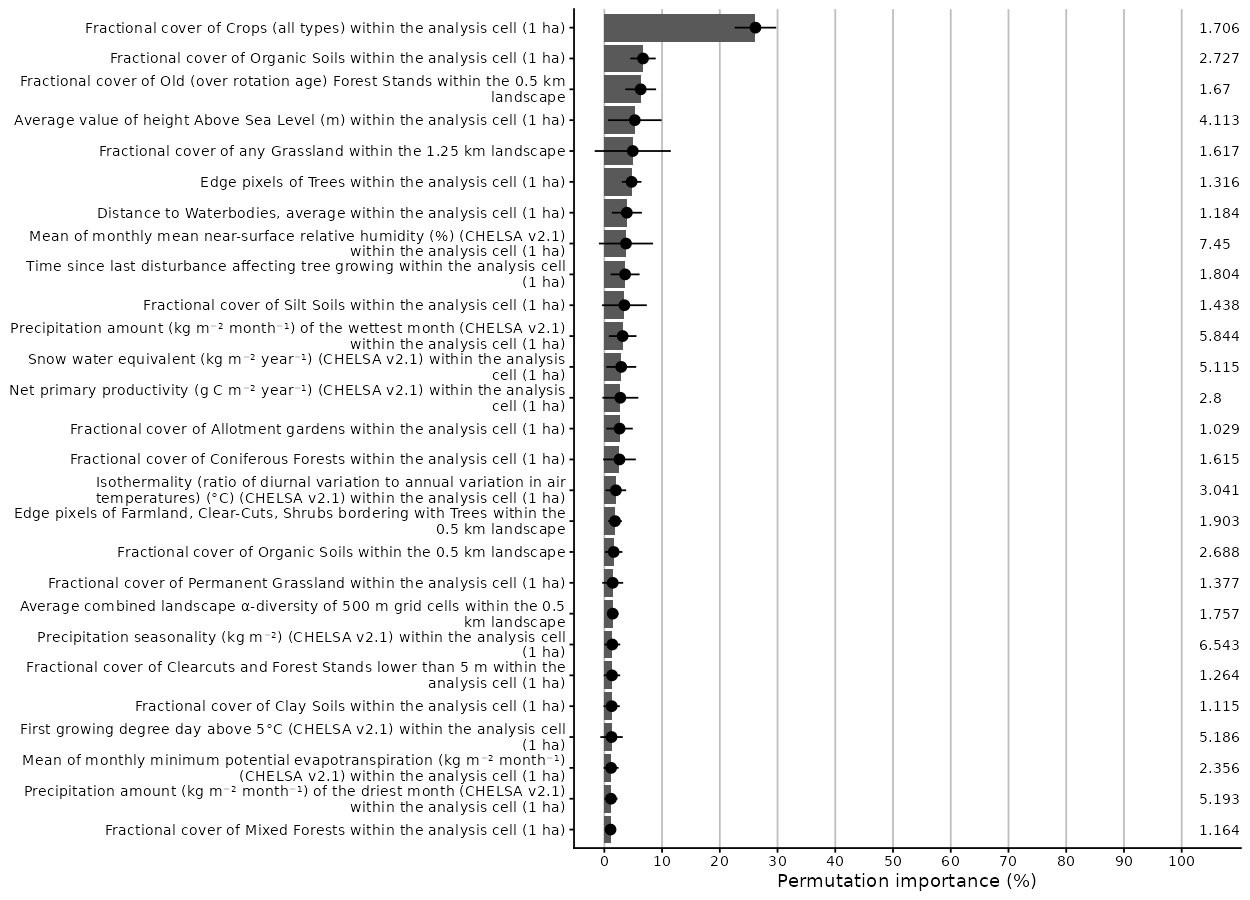
\includegraphics[width=1\linewidth,height=0.70\textheight,keepaspectratio]{results/RANTEMterrestrialv2b1celi/PicVarImpVIFs_RANTEMterrestrial.png}

\par\small\textit{Permutation-importance (mean and standard deviation from 99 permutations, on the x-axis) of the ecogeographical variables (first y-axis, left side), and their variance inflation factor values (second y-axis, right side). **For a full resolution refer to repository: link or online document: link**}\normalsize
\end{center}

\section*{Marginal responses}\label{marginal-responses-16}
\addcontentsline{toc}{section}{Marginal responses}

\begin{center}
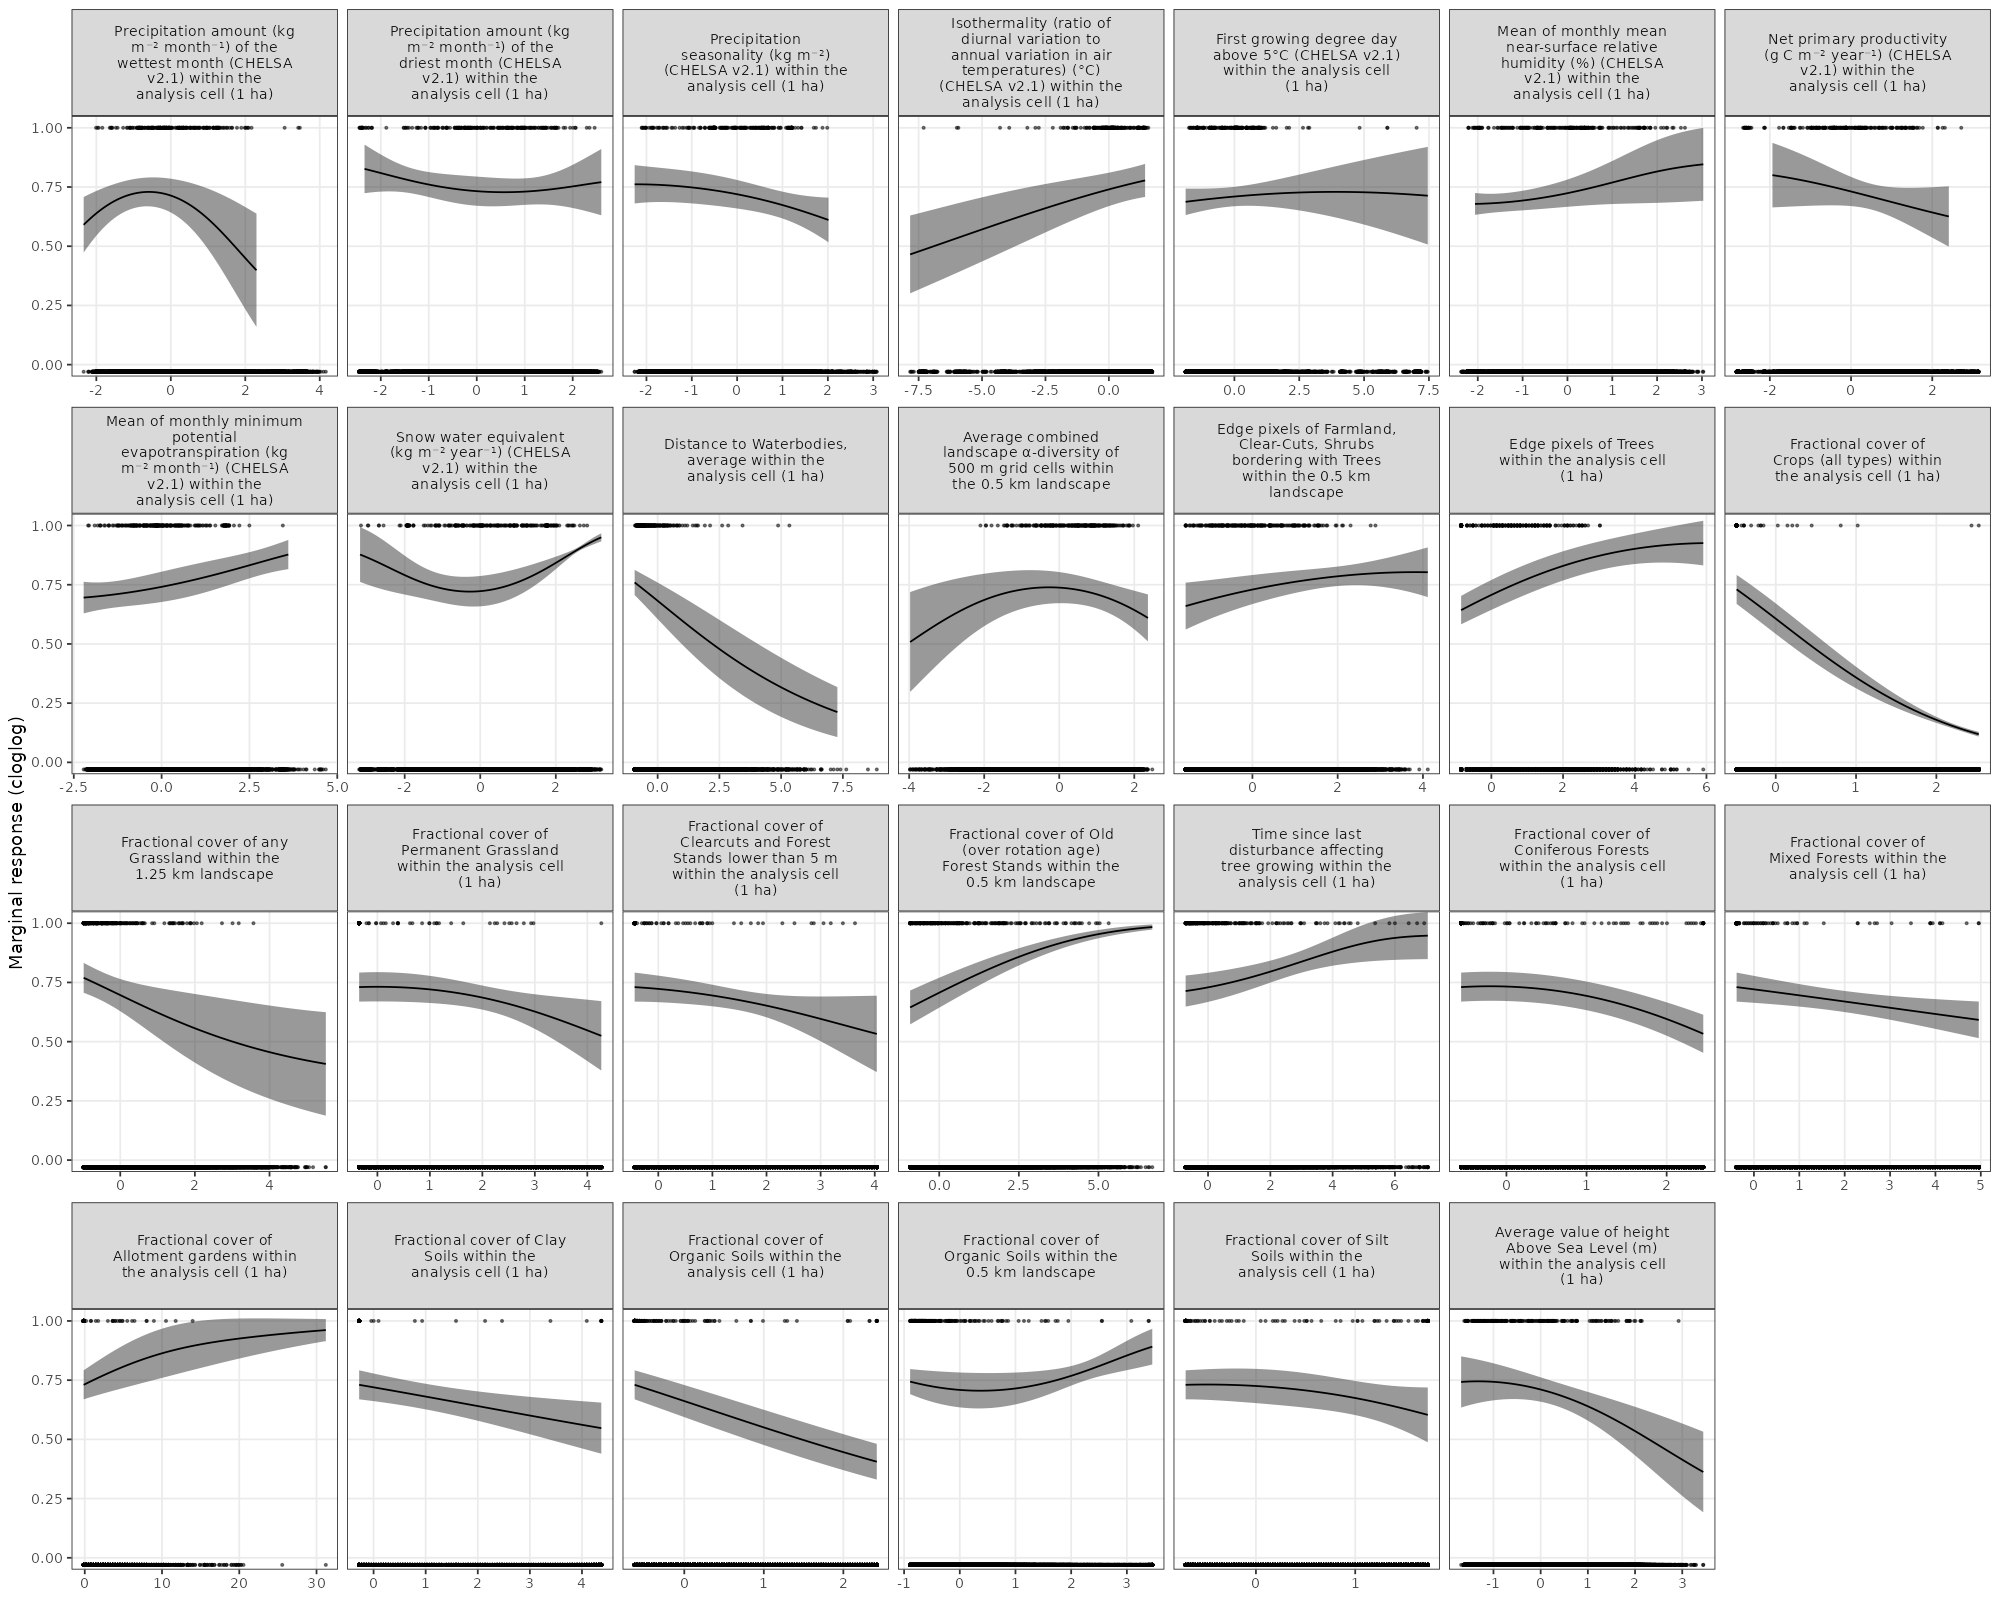
\includegraphics[width=1\linewidth,height=0.70\textheight,keepaspectratio]{results/RANTEMterrestrialv2b1celi/PicMargResp_RANTEMterrestrial.png}

\par\small\textit{Marginalised for arithmetic mean response curves illustrating the effect of each ecogeographical variable on the habitat suitability when all the other variables have their arithmetic mean values. The y-axis shows the predicted habitat suitability (cloglog-transformed), while the x-axis shows the standardised (centred and scaled) value of the ecogeographical variable. Dots at a value of 1 on the y-axis illustrate presence locations in the environment (on the x-axis), while dots at a value of 0 illustrate background locations used in modelling.  **For a full resolution refer to repository: link or online document: link**}\normalsize
\end{center}

\section*{Habitat and conservation associations}\label{habitat-and-conservation-associations-16}
\addcontentsline{toc}{section}{Habitat and conservation associations}

\begin{center}
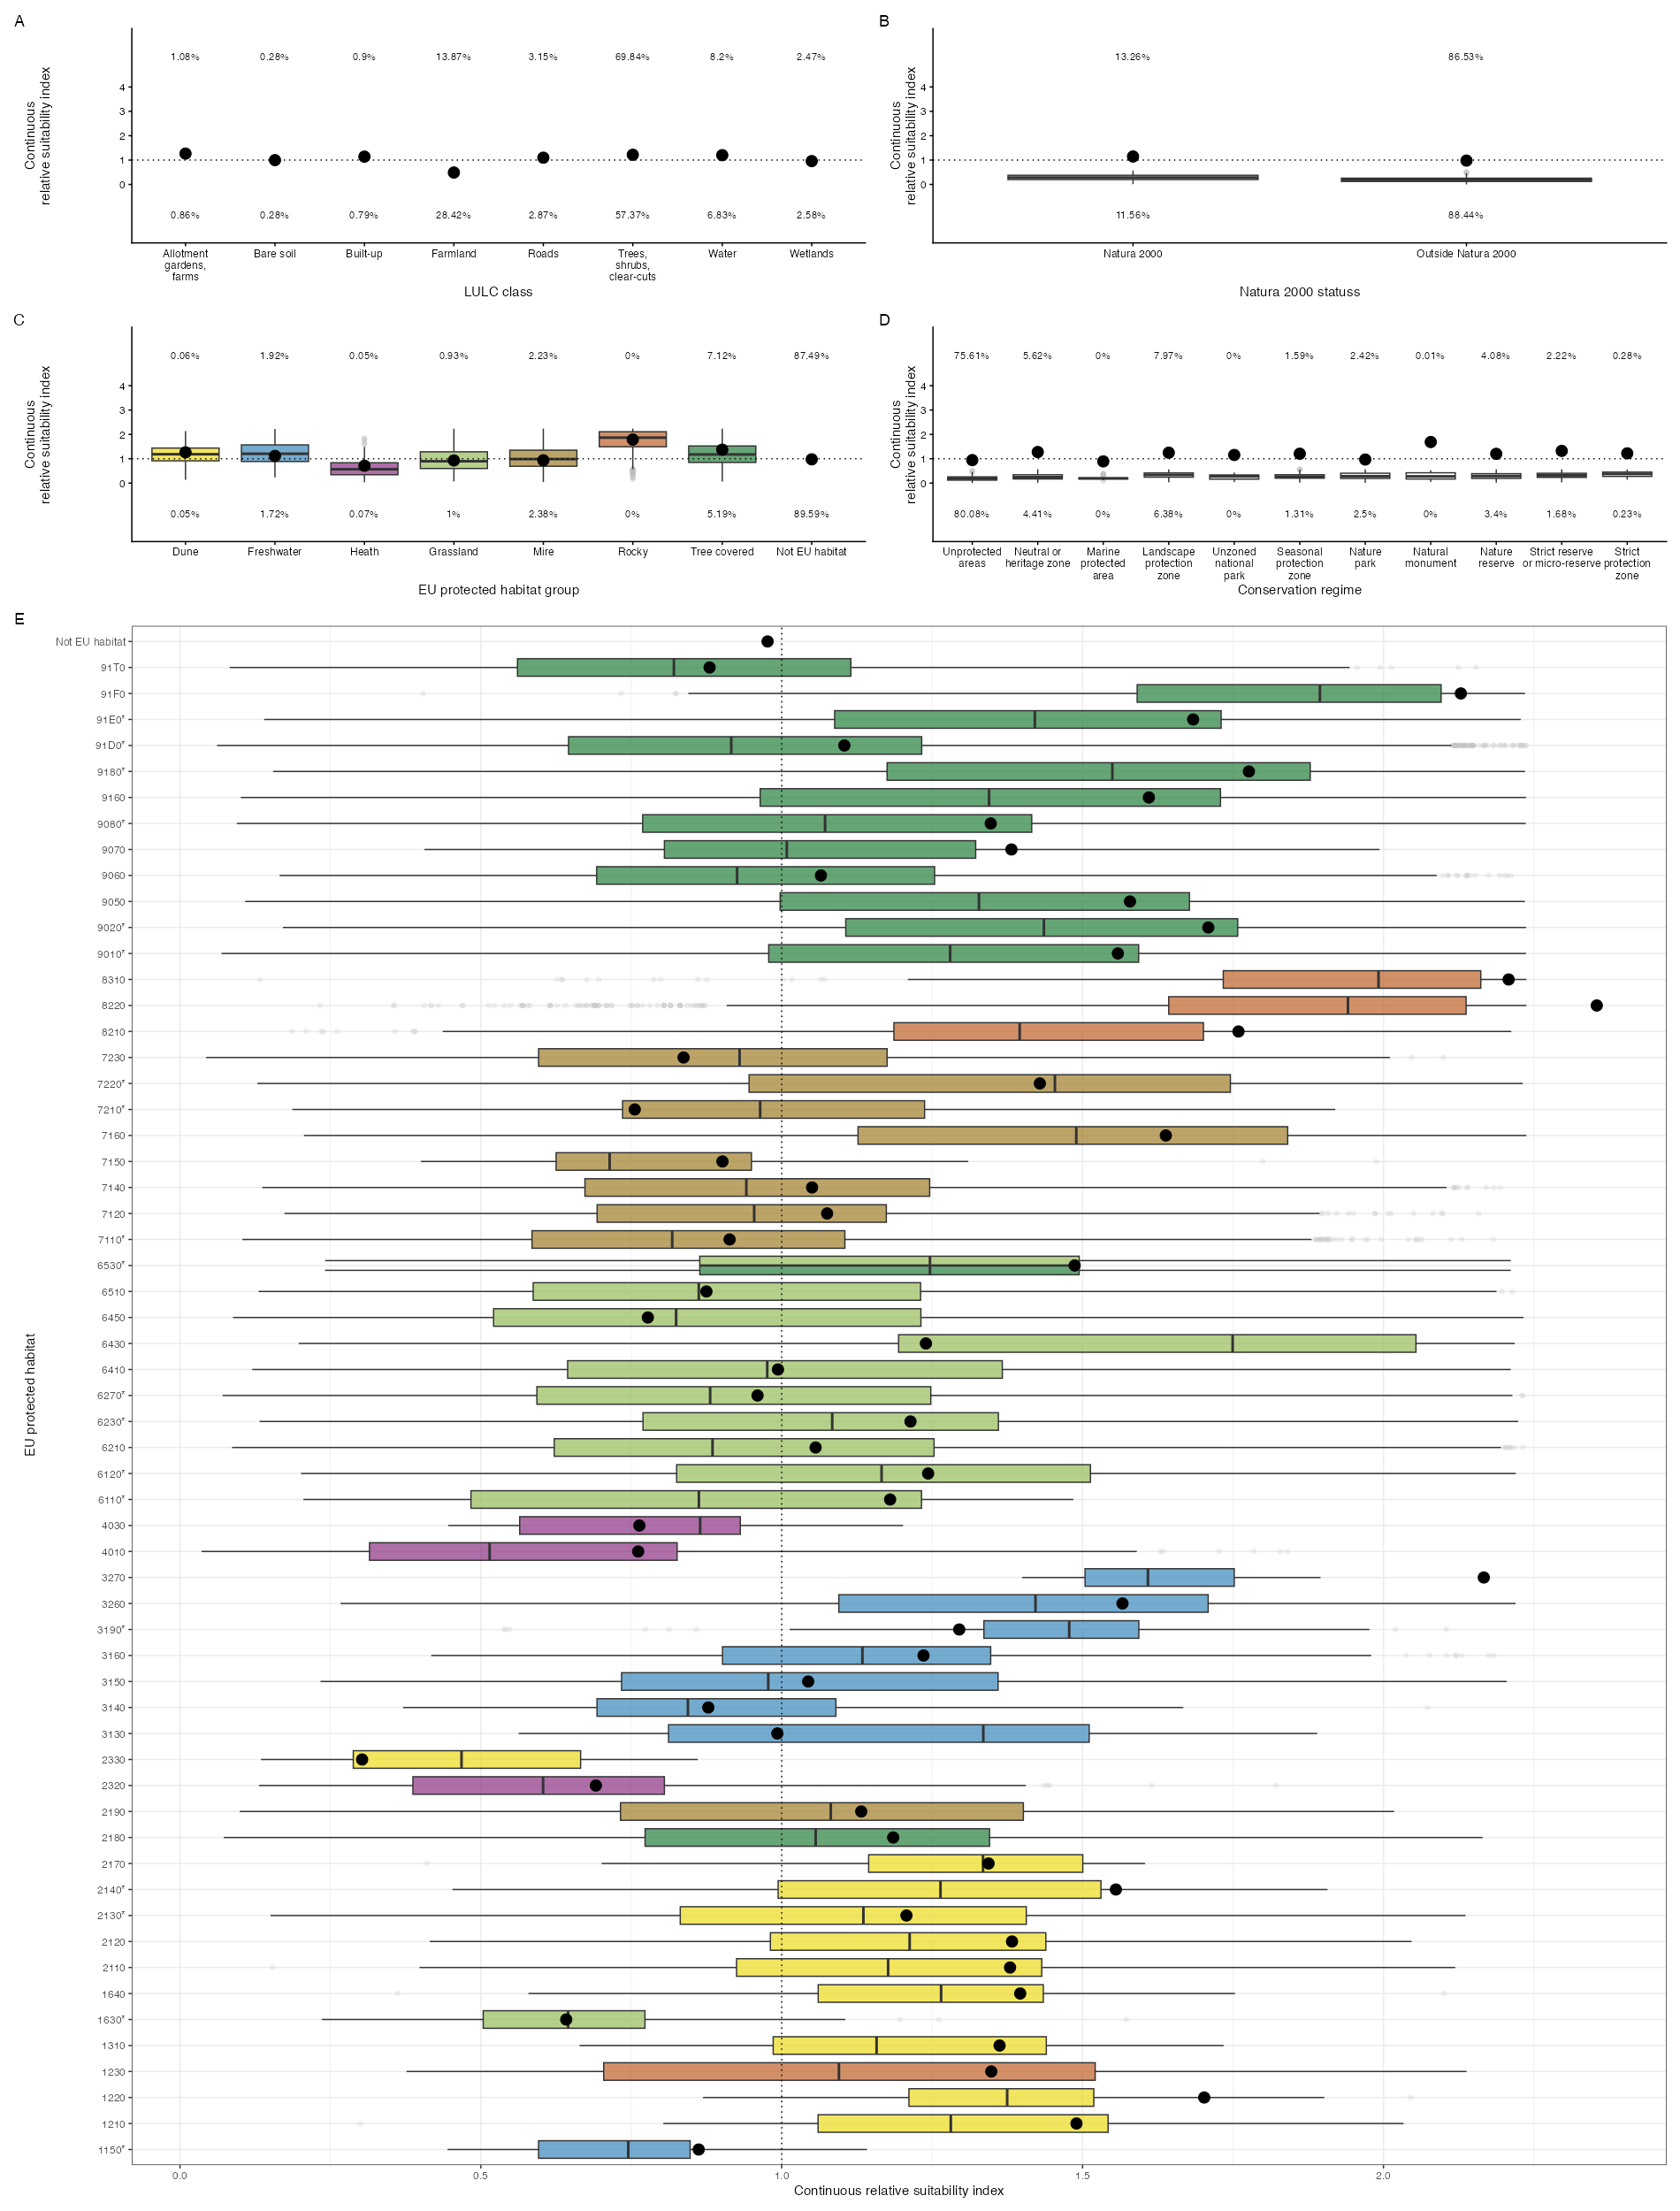
\includegraphics[width=1\linewidth,height=0.70\textheight,keepaspectratio]{results/RANTEMterrestrialv2b1celi/PicAssoc_RANTEMterrestrial.png}

\par\small\textit{Associations between predicted suitability and: (A) land use land cover classes, (B) Natura 2000 status, (C) stratified EU protected habitat classes, (D) conservation regime, and (E) EU protected habitats. The y-axis show continuous relative suitability index (derivative of Manly's index of preference). Colours in (C) and (E) correspond to stratified EU protected habitat classes. For classifications composed of multiple individual polygons, polygon-level indices were additionally calculated to show within-category variation. The figures therefore combine category-level estimates (points) with the distributions of polygon-level values (boxplots, where applicable). Labels above and below the panels report, respectively, the percentage of total predicted suitability and the percentage of mapped area represented by each category. **For a full resolution refer to repository: link or online document: link**}\normalsize
\end{center}

\section*{Conservation prioritization}\label{conservation-prioritization-16}
\addcontentsline{toc}{section}{Conservation prioritization}

\begin{center}
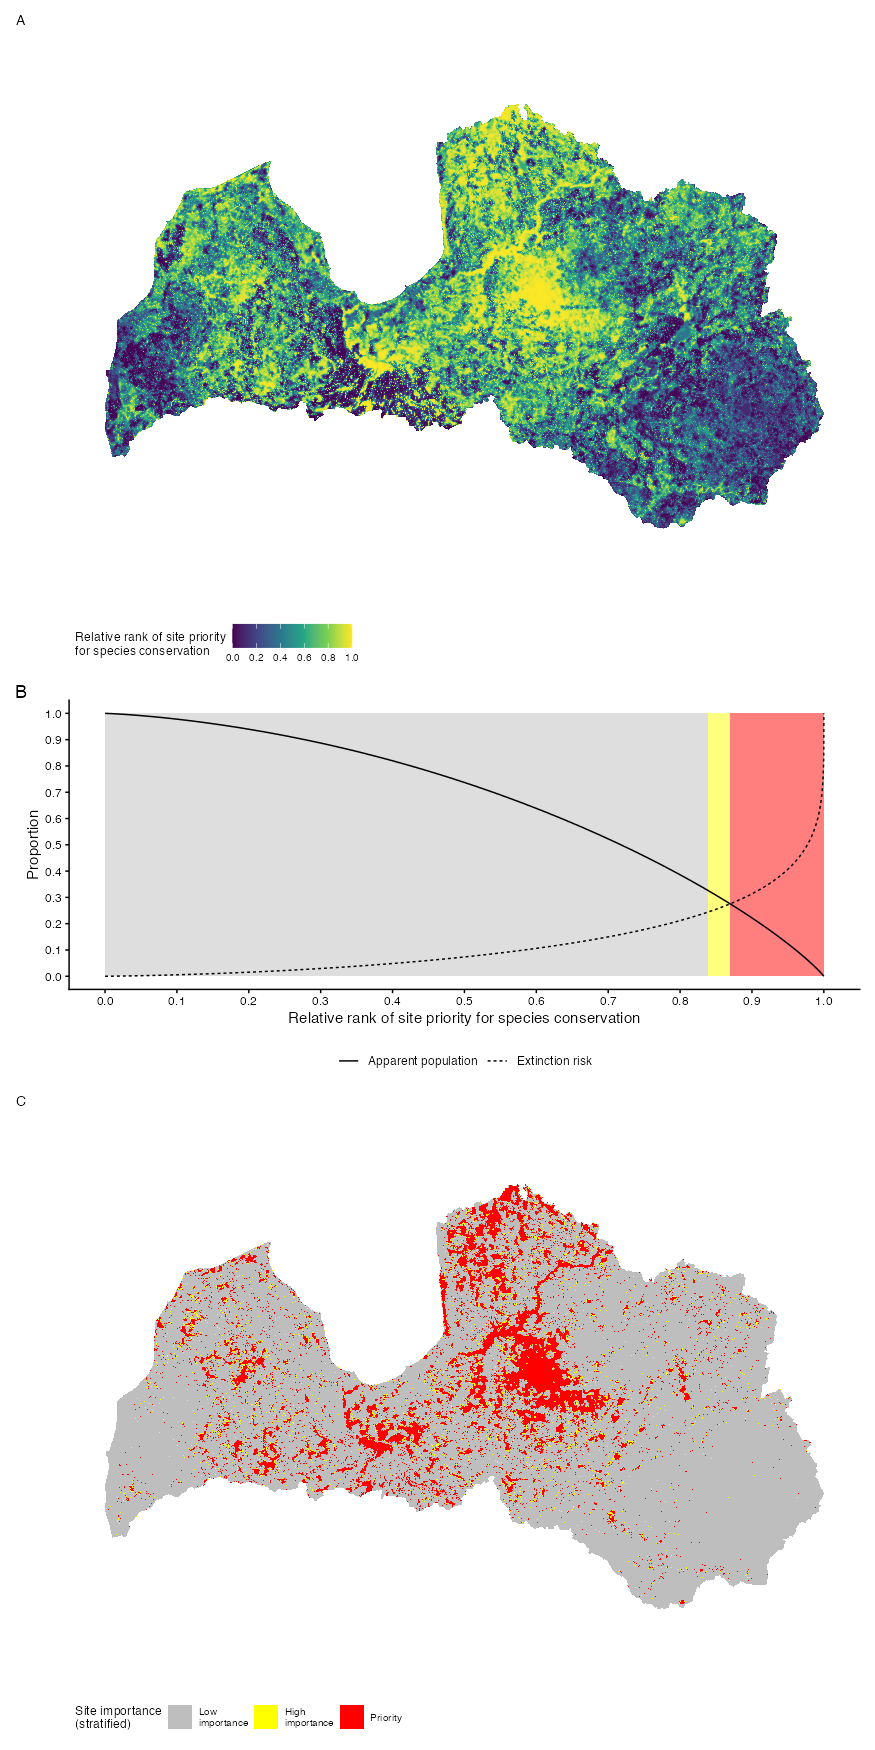
\includegraphics[width=0.85\linewidth,height=0.70\textheight,keepaspectratio]{results/RANTEMterrestrialv2b1celi/PicPrior_RANTEMterrestrial.png}

\par\small\textit{Single-species conservation prioritization focusing on maximisation of core area protection (CAZMAX) while accounting for site connectivity: (A) relative site rank; (B) relationship between apparent-population and extinction-risk curves with a simplified classification which is spatially demonstrated in the bootom row; (C) spatial distribution of proposed classification of site prioritization results. **For a full resolution refer to repository: link or online document: link**}\normalsize
\end{center}

\chapter*{\texorpdfstring{\emph{Rana temporaria} monitoring}{Rana temporaria monitoring}}\label{rantemmonitoring}
\addcontentsline{toc}{chapter}{\emph{Rana temporaria} monitoring}

\section*{Summary}\label{summary-17}
\addcontentsline{toc}{section}{Summary}

\subsection*{Model description}\label{model-description-17}
\addcontentsline{toc}{subsection}{Model description}

Occurrence and background data were divided into model-training with four block spatial cross-validation data and an independent test set. Sampling-bias/background treatment: \textbf{Phenology Weighted Target Group}. Accumulated LULC change within the 1-ha analysis cell was not evaluated; accumulated LULC change within the home-range radius around the analysis cell was not evaluated.

The final data set contained \textbf{761} presence records: \textbf{571} for training with four spatial block cross-validation and \textbf{190} for independent testing. Training background contained \textbf{30014} locations, with \textbf{9986} additional independent-test background locations.

\subsection*{Expert assessment scores}\label{expert-assessment-scores-17}
\addcontentsline{toc}{subsection}{Expert assessment scores}

\begin{itemize}
\tightlist
\item
  \textbf{Marginal responses and variable importance score:} 3 (moderate ecological interpretability)
\item
  \textbf{Map score:} 3 (moderate agreement with known distribution)
\item
  \textbf{Applicability score:} 2 (limited applicability)
\end{itemize}

\textbf{Šo sadaļu aizpildām manuāli no ekspertu aptaujām}

\subsection*{Statistical evaluation}\label{statistical-evaluation-17}
\addcontentsline{toc}{subsection}{Statistical evaluation}

The final model had a training TSS of \textbf{0.401}, with a training-derived cloglog threshold of \textbf{0.424}. Combined training AUC was \textbf{0.816} and combined test AUC was \textbf{0.82}.

\subsubsection*{Spatial cross-validation}\label{spatial-cross-validation-17}
\addcontentsline{toc}{subsubsection}{Spatial cross-validation}

\begin{itemize}
\tightlist
\item
  \textbf{AUC:} 0.8052 ± 0.0375; null models: 0.5246 ± 0.0244; z = 11.4986, p \textless{} 0.001
\item
  \textbf{CBI:} 0.9765 ± 0.0117; null models: 0.1395 ± 0.1708; z = 4.9007, p \textless{} 0.001
\item
  \textbf{OR10:} 0.1331 ± 0.0688; null models: 0.1225 ± 0.0364; z = 0.2926, p = 0.615
\item
  \textbf{ORmin:} 0.0035 ± 0.004; null models: 0.0045 ± 0.0103; z = -0.0991, p = 0.461
\end{itemize}

\subsubsection*{Independent testing}\label{independent-testing-17}
\addcontentsline{toc}{subsubsection}{Independent testing}

\begin{itemize}
\tightlist
\item
  \textbf{TSS:} 0.507; \textbf{sensitivity:} 0.832; \textbf{specificity:} 0.676
\item
  \textbf{AUC:} 0.81; null models: 0.5144 ± 0.0663; z = 4.4525, p \textless{} 0.001
\item
  \textbf{CBI:} 0.989; null models: 0.0759 ± 0.458; z = 1.9936, p = 0.023
\item
  \textbf{OR10:} 0.084; null models: 0.1115 ± 0.0547; z = -0.4993, p = 0.309
\item
  \textbf{ORmin:} 0; null models: 8e-04 ± 0.0023; z = -0.3447, p = 0.365
\end{itemize}

\subsection*{Conservation prioritisation summary}\label{conservation-prioritisation-summary-17}
\addcontentsline{toc}{subsection}{Conservation prioritisation summary}

The primary priority area covers \textbf{12.7\%} of Latvia and contains \textbf{27.6\%} of the summed habitat suitability (apparent population proxy).

The broader high importance area covers \textbf{34\%} of Latvia and contains \textbf{57.9\%} of the summed habitat suitability.

For comparison, the area classified as suitable using the maximum training sensitivity plus specificity habitat-suitability threshold contains \textbf{57.9\%} of the summed continuous habitat suitability.

\subsection*{Version evolution}\label{version-evolution-17}
\addcontentsline{toc}{subsection}{Version evolution}

\textbf{Šo sadaļu aizpildām manuāli, izmntojot sagatavotās shēmas. Jāvienojas par to noformējumu}

\section*{Habitat suitability}\label{habitat-suitability-17}
\addcontentsline{toc}{section}{Habitat suitability}

\begin{center}
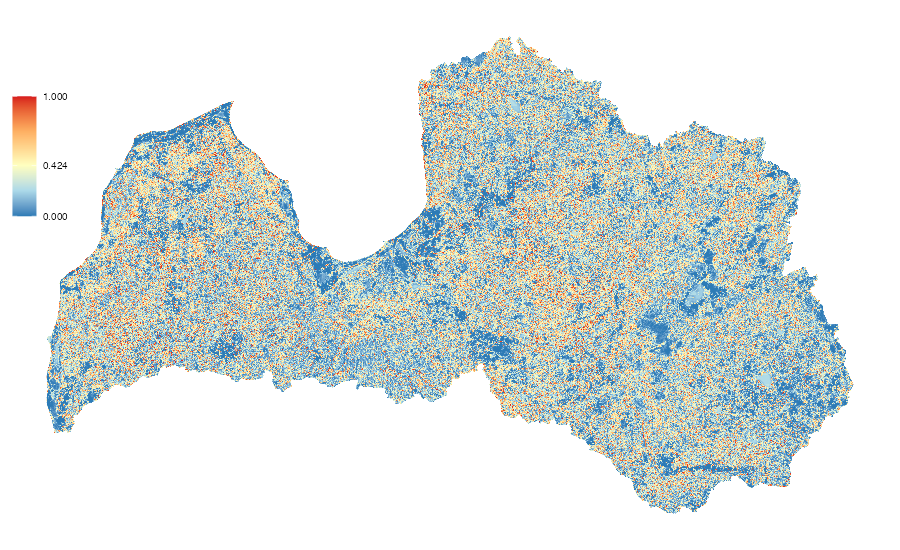
\includegraphics[width=1\linewidth,height=0.70\textheight,keepaspectratio]{results/RANTEMmonitoring_v2b1/PicHSmap_RANTEMmonitoring.png}

\par\small\textit{Predicted continuous habitat suitability across Latvia. The warmer the colour the higher is the predicted habitat suitability. Value in the middle of the legend correspond to the maximum training sensitivity plus specificity threshold. **For a full resolution refer to repository: link or online document: link**}\normalsize
\end{center}

\section*{Model thresholds}\label{model-thresholds-17}
\addcontentsline{toc}{section}{Model thresholds}

Threshold values and associated omission rates

\begin{center}
\resizebox{\linewidth}{!}{%

\begin{tabular}{lrrrrr}
\toprule
Threshold & Cloglog value & Fractional predicted area & Training omission rate & Test omission rate & P-values\\
\midrule
Minimum training presence & 0.0120386 & 0.9631940 & 0.0000000 & 0.0000000 & 0\\
Equal training sensitivity and specificity & 0.5246176 & 0.2548690 & 0.2556918 & 0.0054576 & 0\\
Maximum training sensitivity plus specificity & 0.4240575 & 0.3445897 & 0.1523643 & 0.0031186 & 0\\
Equal test sensitivity and specificity & 0.4989836 & 0.2764904 & 0.2294221 & 0.0047754 & 0\\
Maximum test sensitivity plus specificity & 0.4611386 & 0.3105565 & 0.1961471 & 0.0035084 & 0\\
\bottomrule
\end{tabular}
}
\end{center}

\section*{Variable importance}\label{variable-importance-17}
\addcontentsline{toc}{section}{Variable importance}

\begin{center}
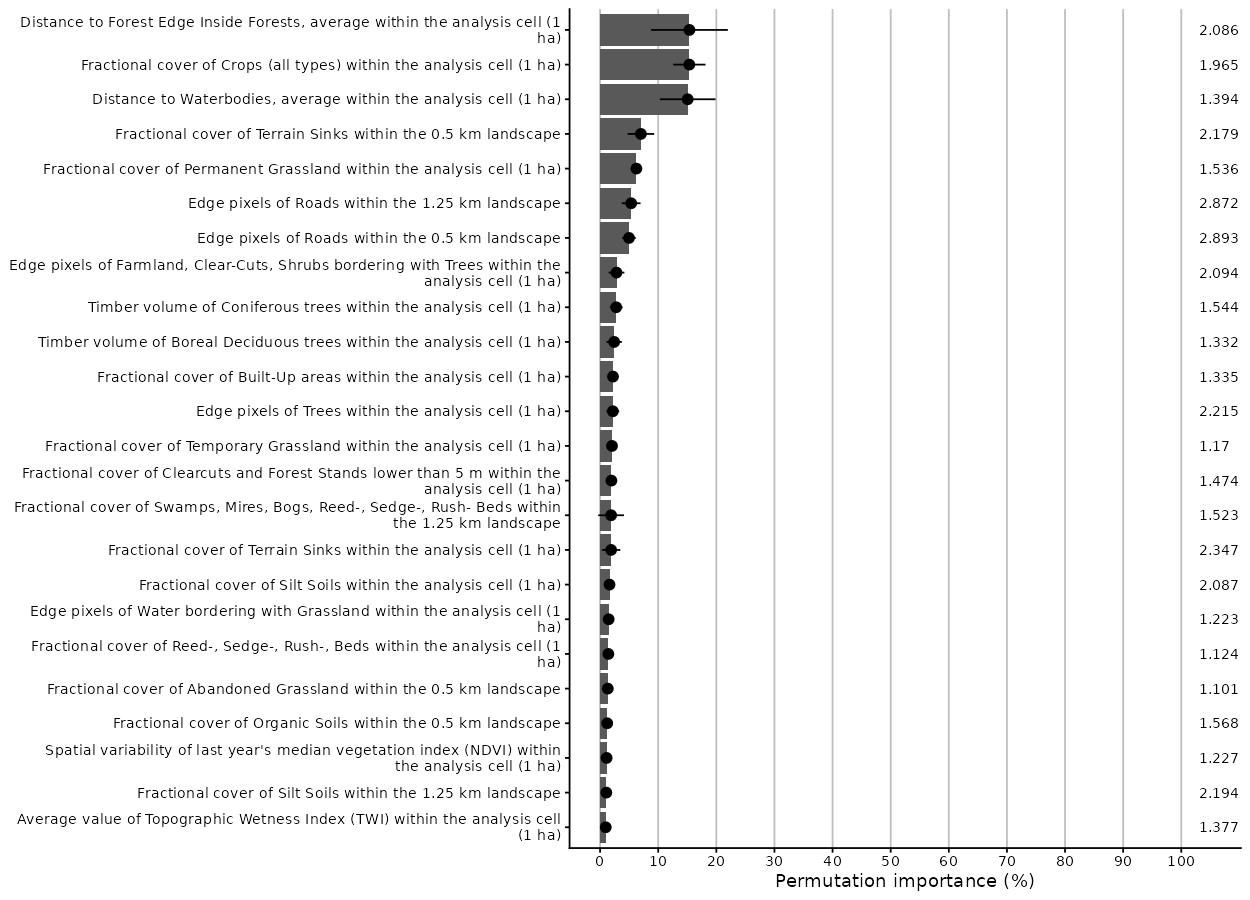
\includegraphics[width=1\linewidth,height=0.70\textheight,keepaspectratio]{results/RANTEMmonitoring_v2b1/PicVarImpVIFs_RANTEMmonitoring.png}

\par\small\textit{Permutation-importance (mean and standard deviation from 99 permutations, on the x-axis) of the ecogeographical variables (first y-axis, left side), and their variance inflation factor values (second y-axis, right side). **For a full resolution refer to repository: link or online document: link**}\normalsize
\end{center}

\section*{Marginal responses}\label{marginal-responses-17}
\addcontentsline{toc}{section}{Marginal responses}

\begin{center}
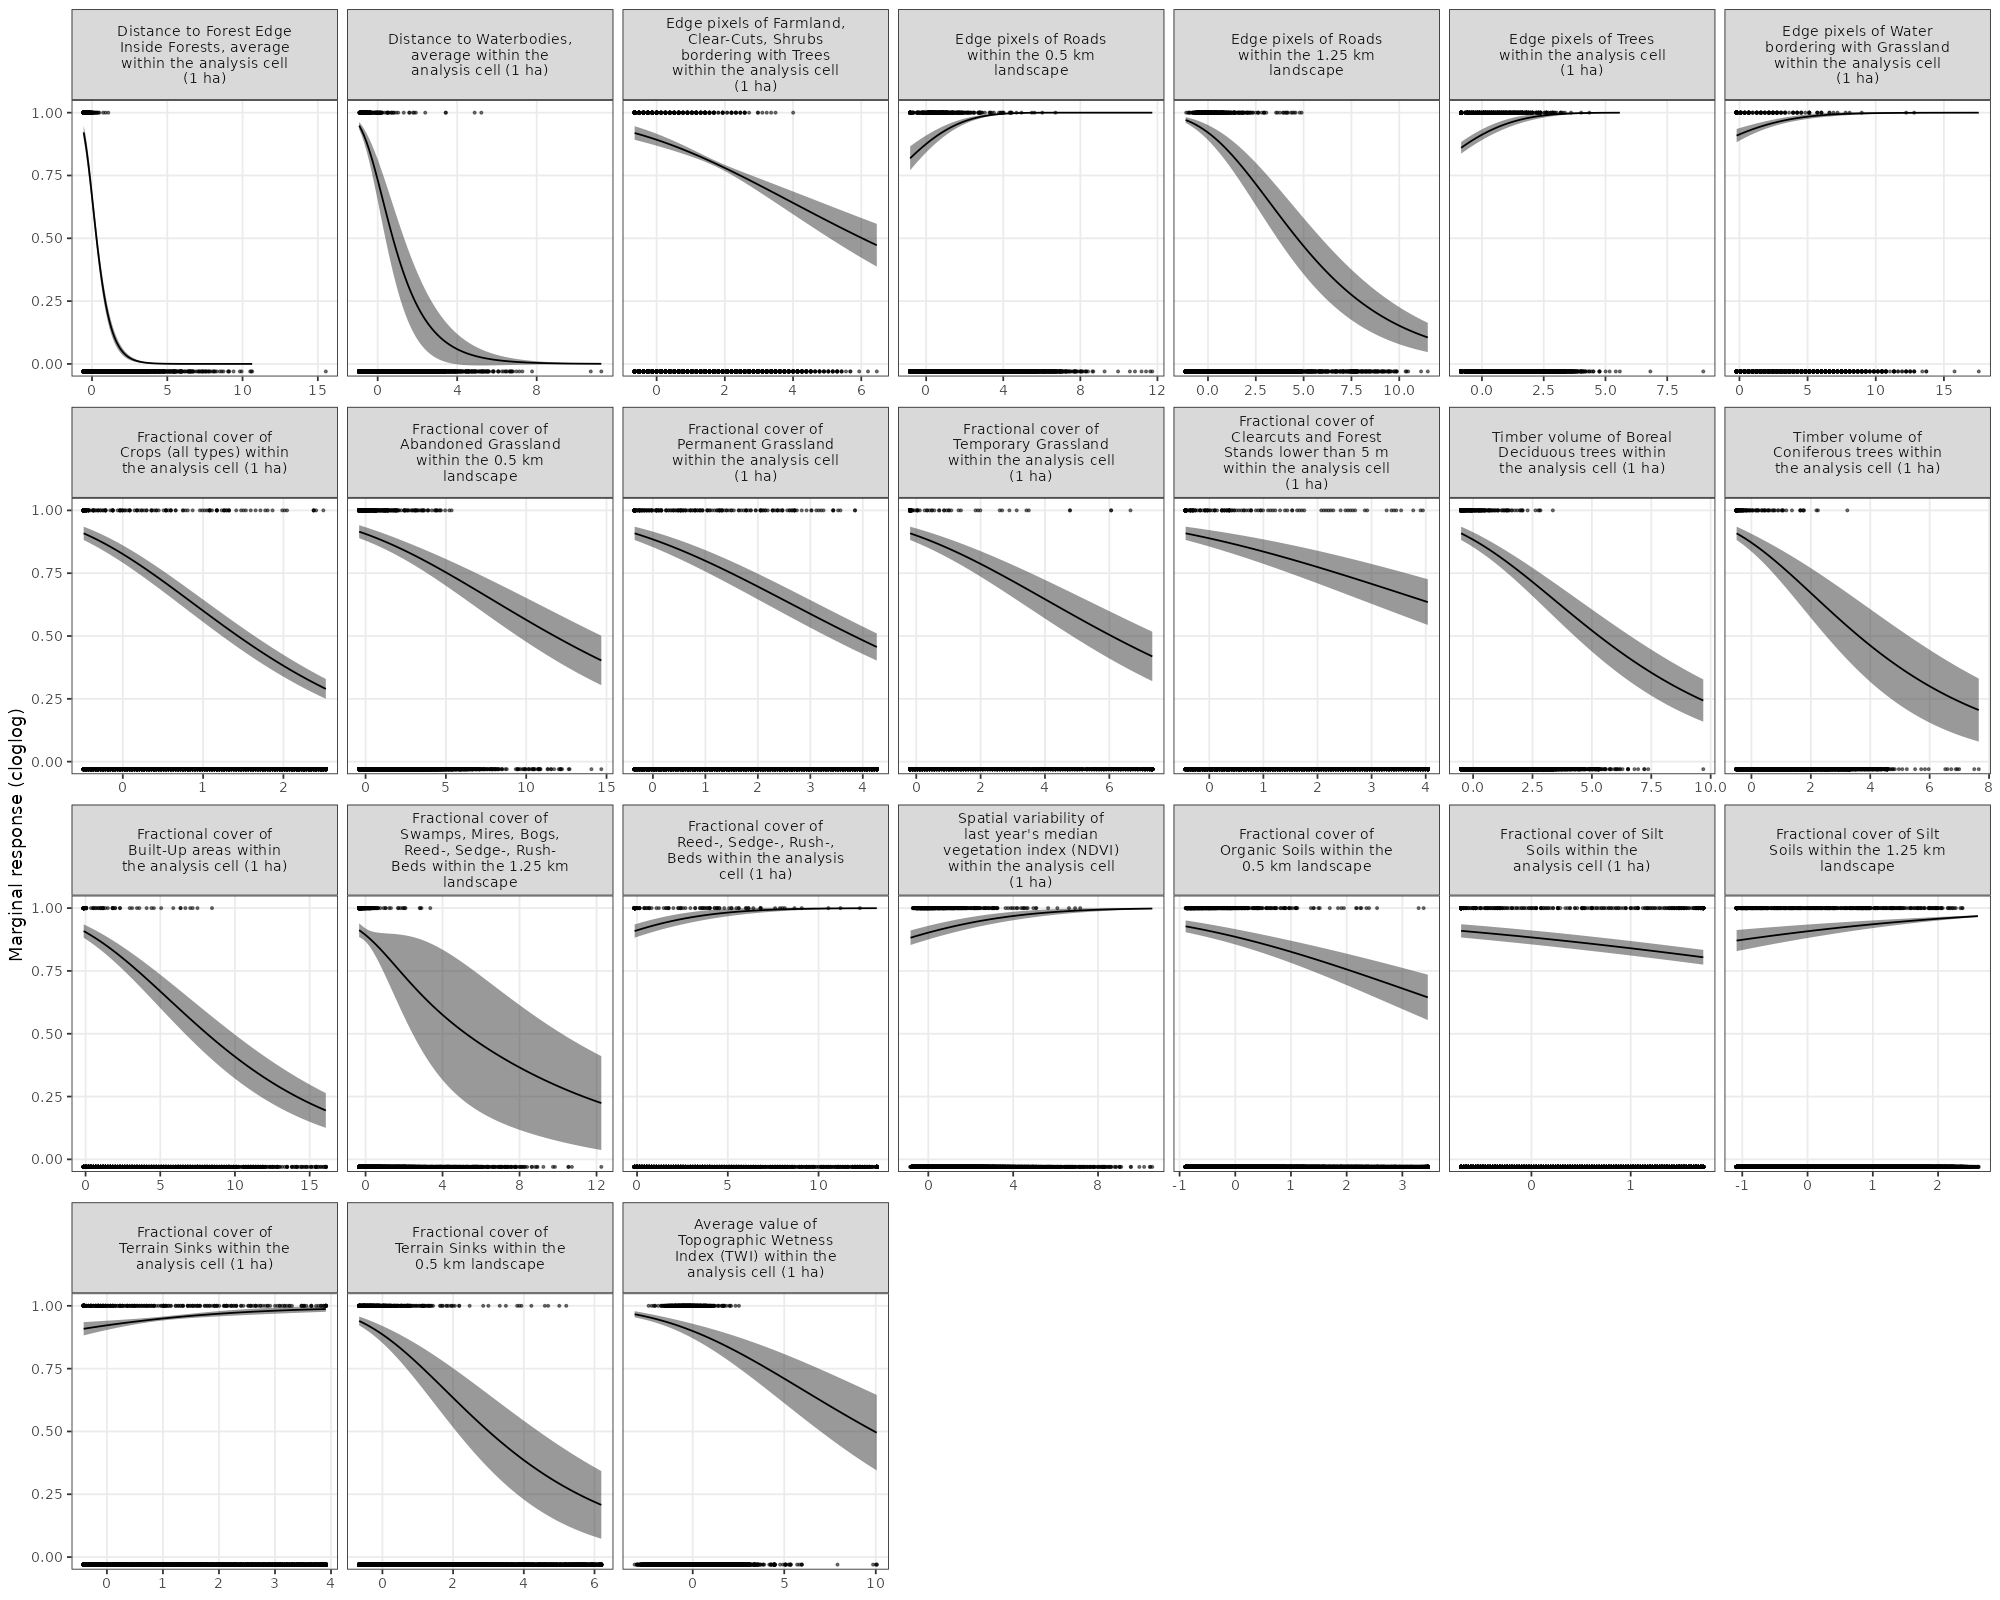
\includegraphics[width=1\linewidth,height=0.70\textheight,keepaspectratio]{results/RANTEMmonitoring_v2b1/PicMargResp_RANTEMmonitoring.png}

\par\small\textit{Marginalised for arithmetic mean response curves illustrating the effect of each ecogeographical variable on the habitat suitability when all the other variables have their arithmetic mean values. The y-axis shows the predicted habitat suitability (cloglog-transformed), while the x-axis shows the standardised (centred and scaled) value of the ecogeographical variable. Dots at a value of 1 on the y-axis illustrate presence locations in the environment (on the x-axis), while dots at a value of 0 illustrate background locations used in modelling.  **For a full resolution refer to repository: link or online document: link**}\normalsize
\end{center}

\section*{Habitat and conservation associations}\label{habitat-and-conservation-associations-17}
\addcontentsline{toc}{section}{Habitat and conservation associations}

\begin{center}
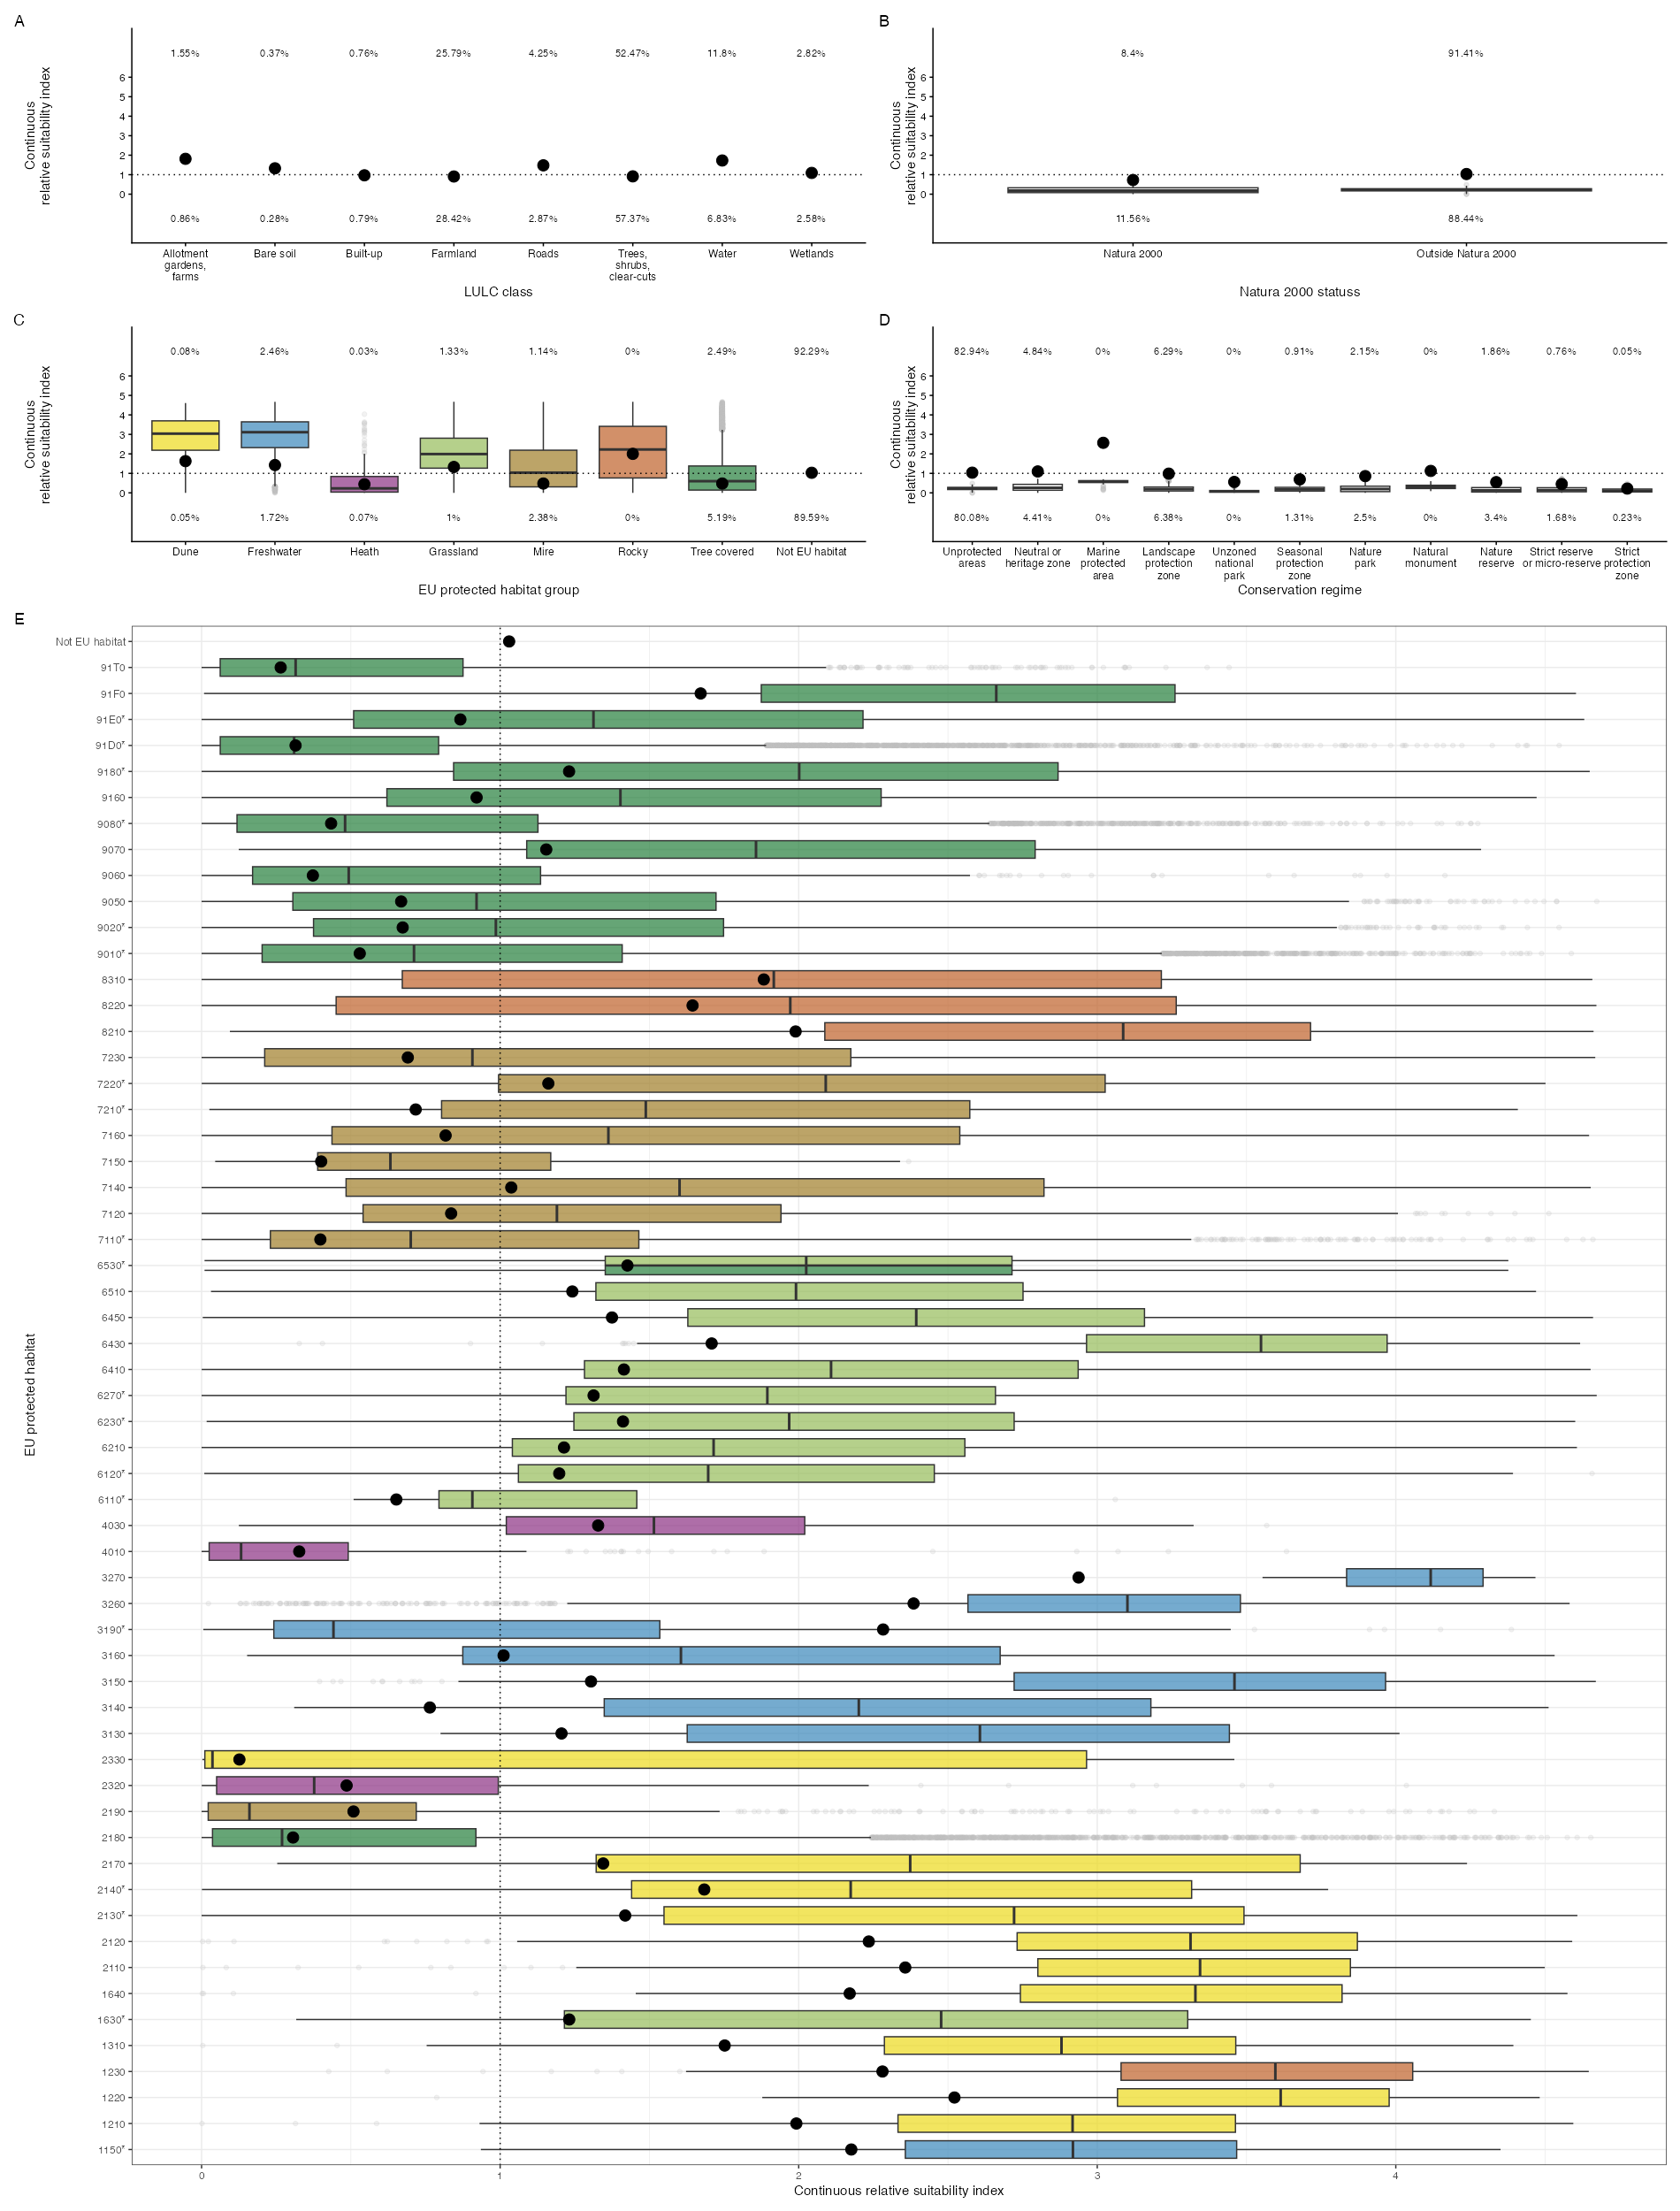
\includegraphics[width=1\linewidth,height=0.70\textheight,keepaspectratio]{results/RANTEMmonitoring_v2b1/PicAssoc_RANTEMmonitoring.png}

\par\small\textit{Associations between predicted suitability and: (A) land use land cover classes, (B) Natura 2000 status, (C) stratified EU protected habitat classes, (D) conservation regime, and (E) EU protected habitats. The y-axis show continuous relative suitability index (derivative of Manly's index of preference). Colours in (C) and (E) correspond to stratified EU protected habitat classes. For classifications composed of multiple individual polygons, polygon-level indices were additionally calculated to show within-category variation. The figures therefore combine category-level estimates (points) with the distributions of polygon-level values (boxplots, where applicable). Labels above and below the panels report, respectively, the percentage of total predicted suitability and the percentage of mapped area represented by each category. **For a full resolution refer to repository: link or online document: link**}\normalsize
\end{center}

\section*{Conservation prioritization}\label{conservation-prioritization-17}
\addcontentsline{toc}{section}{Conservation prioritization}

\begin{center}
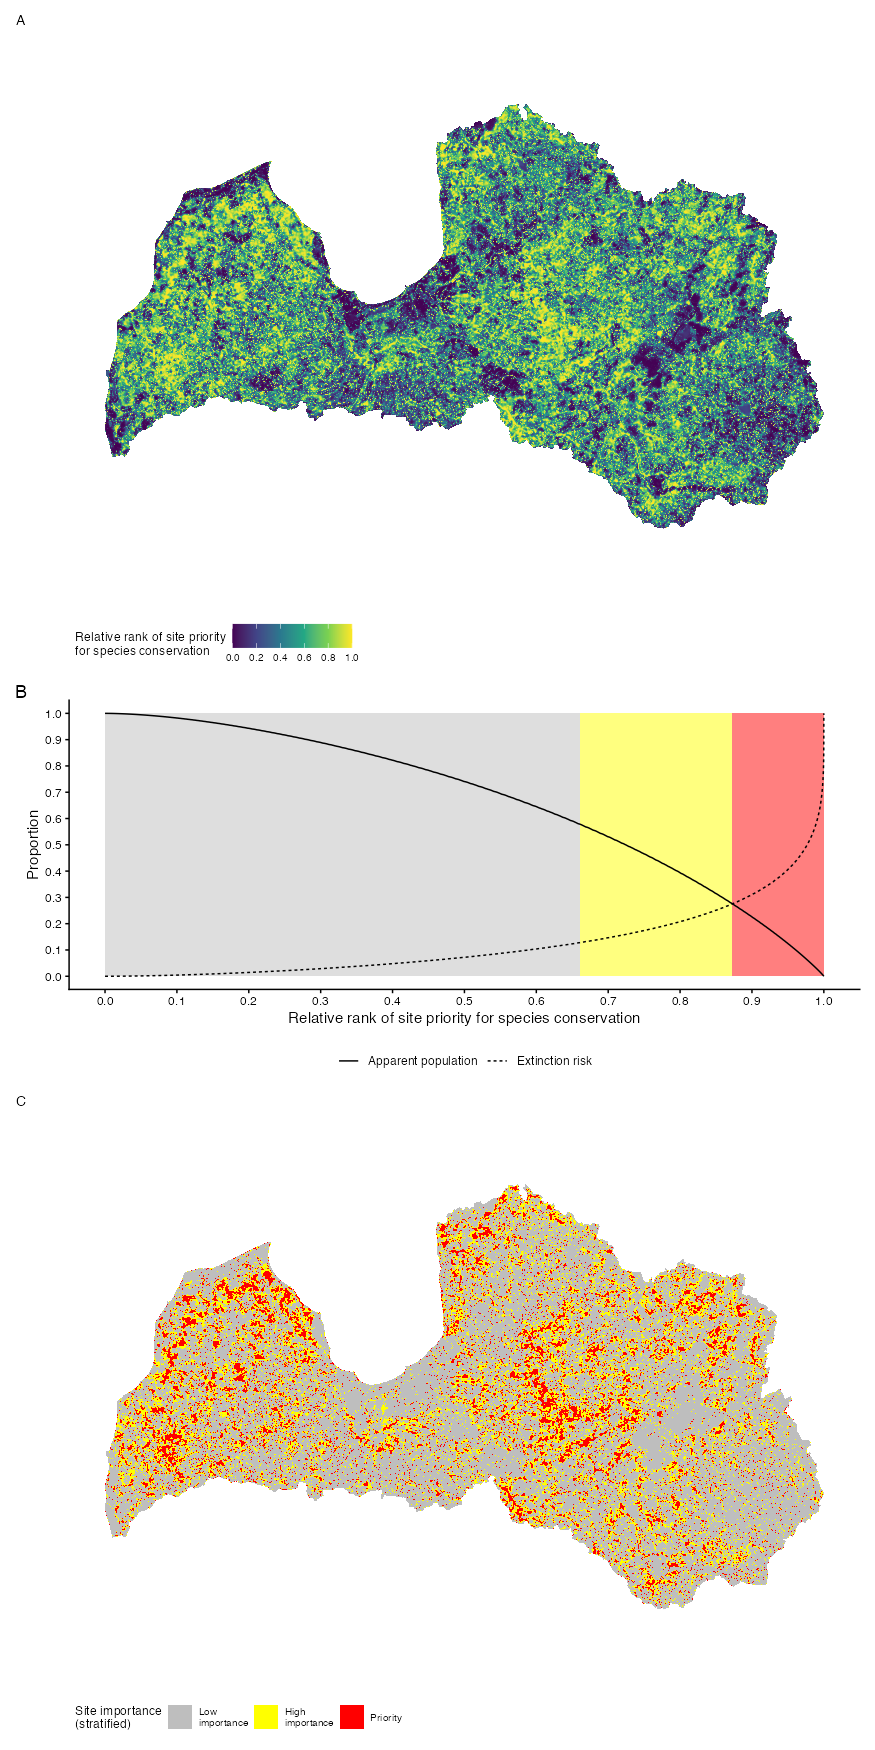
\includegraphics[width=0.85\linewidth,height=0.70\textheight,keepaspectratio]{results/RANTEMmonitoring_v2b1/PicPrior_RANTEMmonitoring.png}

\par\small\textit{Single-species conservation prioritization focusing on maximisation of core area protection (CAZMAX) while accounting for site connectivity: (A) relative site rank; (B) relationship between apparent-population and extinction-risk curves with a simplified classification which is spatially demonstrated in the bootom row; (C) spatial distribution of proposed classification of site prioritization results. **For a full resolution refer to repository: link or online document: link**}\normalsize
\end{center}

\chapter*{\texorpdfstring{\emph{Rana arvalis}}{Rana arvalis}}\label{ranarv}
\addcontentsline{toc}{chapter}{\emph{Rana arvalis}}

\section*{Summary}\label{summary-18}
\addcontentsline{toc}{section}{Summary}

\subsection*{Model description}\label{model-description-18}
\addcontentsline{toc}{subsection}{Model description}

Occurrence and background data were divided into model-training with four block spatial cross-validation data and an independent test set. Sampling-bias/background treatment: \textbf{Phenology Weighted Target Group}. Observations were retained only where accumulated LULC change within the 1-ha analysis cell from the year of observation to 2024 did not exceed 50\%; observations were retained only where accumulated LULC change within the home-range radius around the analysis cell from the year of observation to 2024 did not exceed 50\%.

The final data set contained \textbf{450} presence records: \textbf{338} for training with four spatial block cross-validation and \textbf{112} for independent testing. Training background contained \textbf{30049} locations, with \textbf{9951} additional independent-test background locations.

\subsection*{Expert assessment scores}\label{expert-assessment-scores-18}
\addcontentsline{toc}{subsection}{Expert assessment scores}

\begin{itemize}
\tightlist
\item
  \textbf{Marginal responses and variable importance score:} 3 (moderate ecological interpretability)
\item
  \textbf{Map score:} 3 (moderate agreement with known distribution)
\item
  \textbf{Applicability score:} 2 (limited applicability)
\end{itemize}

\textbf{Šo sadaļu aizpildām manuāli no ekspertu aptaujām}

\subsection*{Statistical evaluation}\label{statistical-evaluation-18}
\addcontentsline{toc}{subsection}{Statistical evaluation}

The final model had a training TSS of \textbf{0.401}, with a training-derived cloglog threshold of \textbf{0.42}. Combined training AUC was \textbf{0.798} and combined test AUC was \textbf{0.778}.

\subsubsection*{Spatial cross-validation}\label{spatial-cross-validation-18}
\addcontentsline{toc}{subsubsection}{Spatial cross-validation}

\begin{itemize}
\tightlist
\item
  \textbf{AUC:} 0.7856 ± 0.0139; null models: 0.5152 ± 0.0224; z = 12.0719, p \textless{} 0.001
\item
  \textbf{CBI:} 0.9558 ± 0.0161; null models: 0.1015 ± 0.1387; z = 6.1605, p \textless{} 0.001
\item
  \textbf{OR10:} 0.1241 ± 0.0528; null models: 0.1071 ± 0.0427; z = 0.3984, p = 0.655
\item
  \textbf{ORmin:} 0.0029 ± 0.0059; null models: 0.0047 ± 0.01; z = -0.175, p = 0.431
\end{itemize}

\subsubsection*{Independent testing}\label{independent-testing-18}
\addcontentsline{toc}{subsubsection}{Independent testing}

\begin{itemize}
\tightlist
\item
  \textbf{TSS:} 0.444; \textbf{sensitivity:} 0.812; \textbf{specificity:} 0.632
\item
  \textbf{AUC:} 0.768; null models: 0.5126 ± 0.0727; z = 3.5149, p \textless{} 0.001
\item
  \textbf{CBI:} 0.973; null models: 0.085 ± 0.4761; z = 1.8651, p = 0.031
\item
  \textbf{OR10:} 0.116; null models: 0.0931 ± 0.0648; z = 0.354, p = 0.638
\item
  \textbf{ORmin:} 0; null models: 0.0036 ± 0.0097; z = -0.3664, p = 0.357
\end{itemize}

\subsection*{Conservation prioritisation summary}\label{conservation-prioritisation-summary-18}
\addcontentsline{toc}{subsection}{Conservation prioritisation summary}

The primary priority area covers \textbf{16.3\%} of Latvia and contains \textbf{27.6\%} of the summed habitat suitability (apparent population proxy).

The broader high importance area covers \textbf{38.1\%} of Latvia and contains \textbf{53.4\%} of the summed habitat suitability.

For comparison, the area classified as suitable using the maximum training sensitivity plus specificity habitat-suitability threshold contains \textbf{53.4\%} of the summed continuous habitat suitability.

\subsection*{Version evolution}\label{version-evolution-18}
\addcontentsline{toc}{subsection}{Version evolution}

\textbf{Šo sadaļu aizpildām manuāli, izmntojot sagatavotās shēmas. Jāvienojas par to noformējumu}

\section*{Habitat suitability}\label{habitat-suitability-18}
\addcontentsline{toc}{section}{Habitat suitability}

\begin{center}
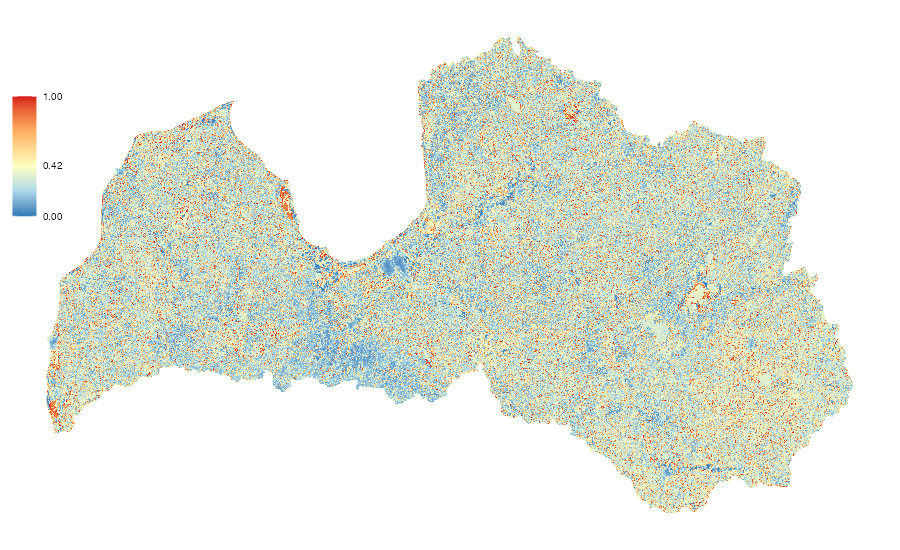
\includegraphics[width=1\linewidth,height=0.70\textheight,keepaspectratio]{results/RANARVv4a1/PicHSmap_RANARV.png}

\par\small\textit{Predicted continuous habitat suitability across Latvia. The warmer the colour the higher is the predicted habitat suitability. Value in the middle of the legend correspond to the maximum training sensitivity plus specificity threshold. **For a full resolution refer to repository: link or online document: link**}\normalsize
\end{center}

\section*{Model thresholds}\label{model-thresholds-18}
\addcontentsline{toc}{section}{Model thresholds}

Threshold values and associated omission rates

\begin{center}
\resizebox{\linewidth}{!}{%

\begin{tabular}{lrrrrr}
\toprule
Threshold & Cloglog value & Fractional predicted area & Training omission rate & Test omission rate & P-values\\
\midrule
Minimum training presence & 0.1238001 & 0.9425744 & 0.0000000 & 0.0000000 & 0\\
Equal training sensitivity and specificity & 0.5059491 & 0.2810711 & 0.2810651 & 0.0036579 & 0\\
Maximum training sensitivity plus specificity & 0.4202450 & 0.3848012 & 0.1508876 & 0.0020761 & 0\\
Equal test sensitivity and specificity & 0.4736589 & 0.3161553 & 0.2396450 & 0.0033613 & 0\\
Maximum test sensitivity plus specificity & 0.4034181 & 0.4108496 & 0.1390533 & 0.0015818 & 0\\
\bottomrule
\end{tabular}
}
\end{center}

\section*{Variable importance}\label{variable-importance-18}
\addcontentsline{toc}{section}{Variable importance}

\begin{center}
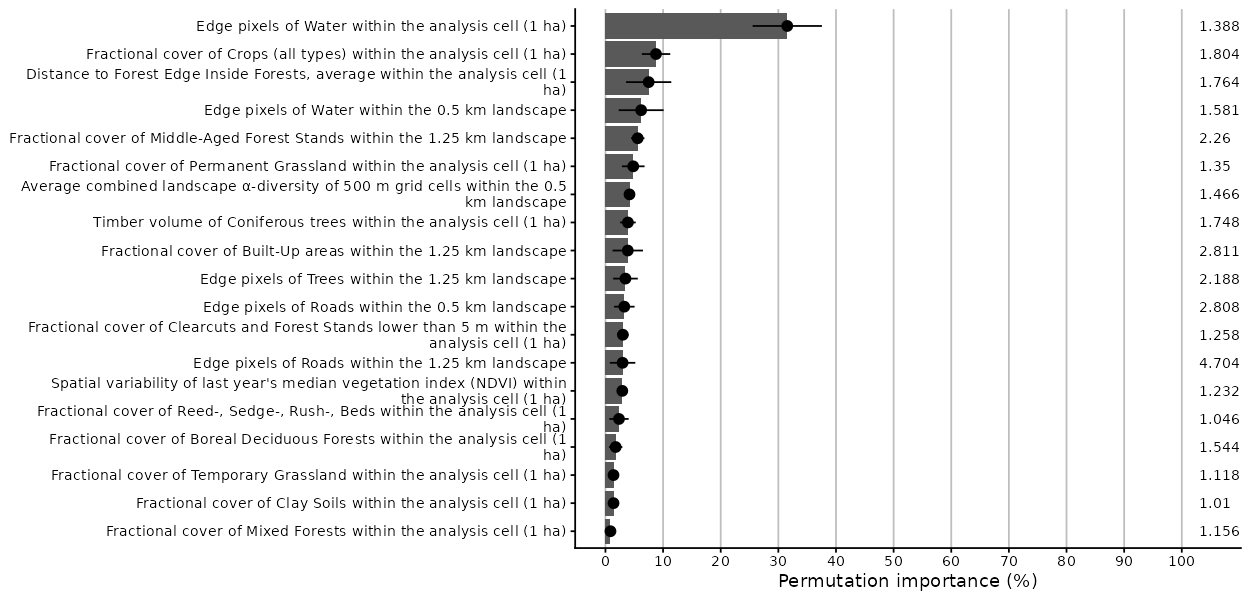
\includegraphics[width=1\linewidth,height=0.70\textheight,keepaspectratio]{results/RANARVv4a1/PicVarImpVIFs_RANARV.png}

\par\small\textit{Permutation-importance (mean and standard deviation from 99 permutations, on the x-axis) of the ecogeographical variables (first y-axis, left side), and their variance inflation factor values (second y-axis, right side). **For a full resolution refer to repository: link or online document: link**}\normalsize
\end{center}

\section*{Marginal responses}\label{marginal-responses-18}
\addcontentsline{toc}{section}{Marginal responses}

\begin{center}
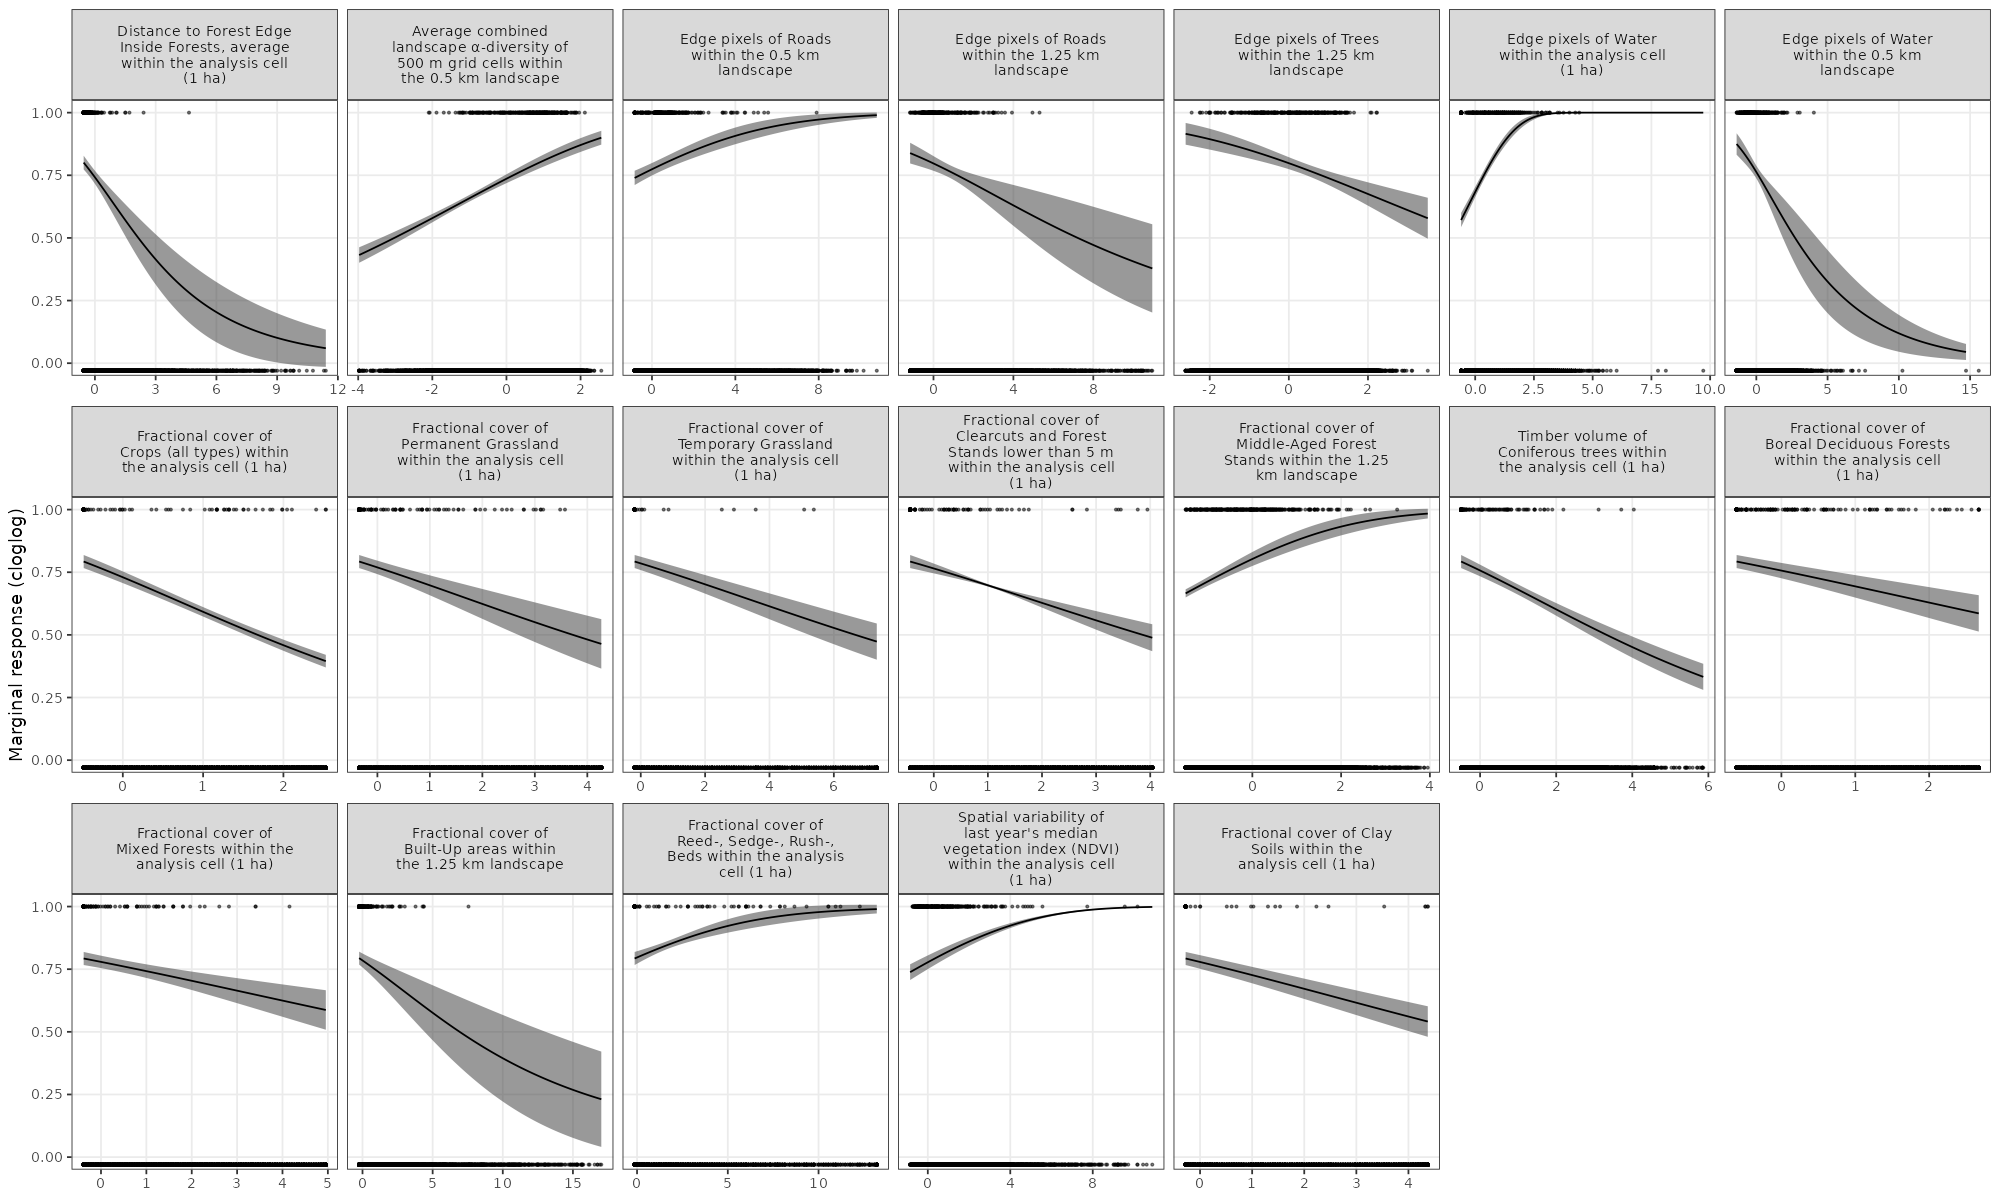
\includegraphics[width=1\linewidth,height=0.70\textheight,keepaspectratio]{results/RANARVv4a1/PicMargResp_RANARV.png}

\par\small\textit{Marginalised for arithmetic mean response curves illustrating the effect of each ecogeographical variable on the habitat suitability when all the other variables have their arithmetic mean values. The y-axis shows the predicted habitat suitability (cloglog-transformed), while the x-axis shows the standardised (centred and scaled) value of the ecogeographical variable. Dots at a value of 1 on the y-axis illustrate presence locations in the environment (on the x-axis), while dots at a value of 0 illustrate background locations used in modelling.  **For a full resolution refer to repository: link or online document: link**}\normalsize
\end{center}

\section*{Habitat and conservation associations}\label{habitat-and-conservation-associations-18}
\addcontentsline{toc}{section}{Habitat and conservation associations}

\begin{center}
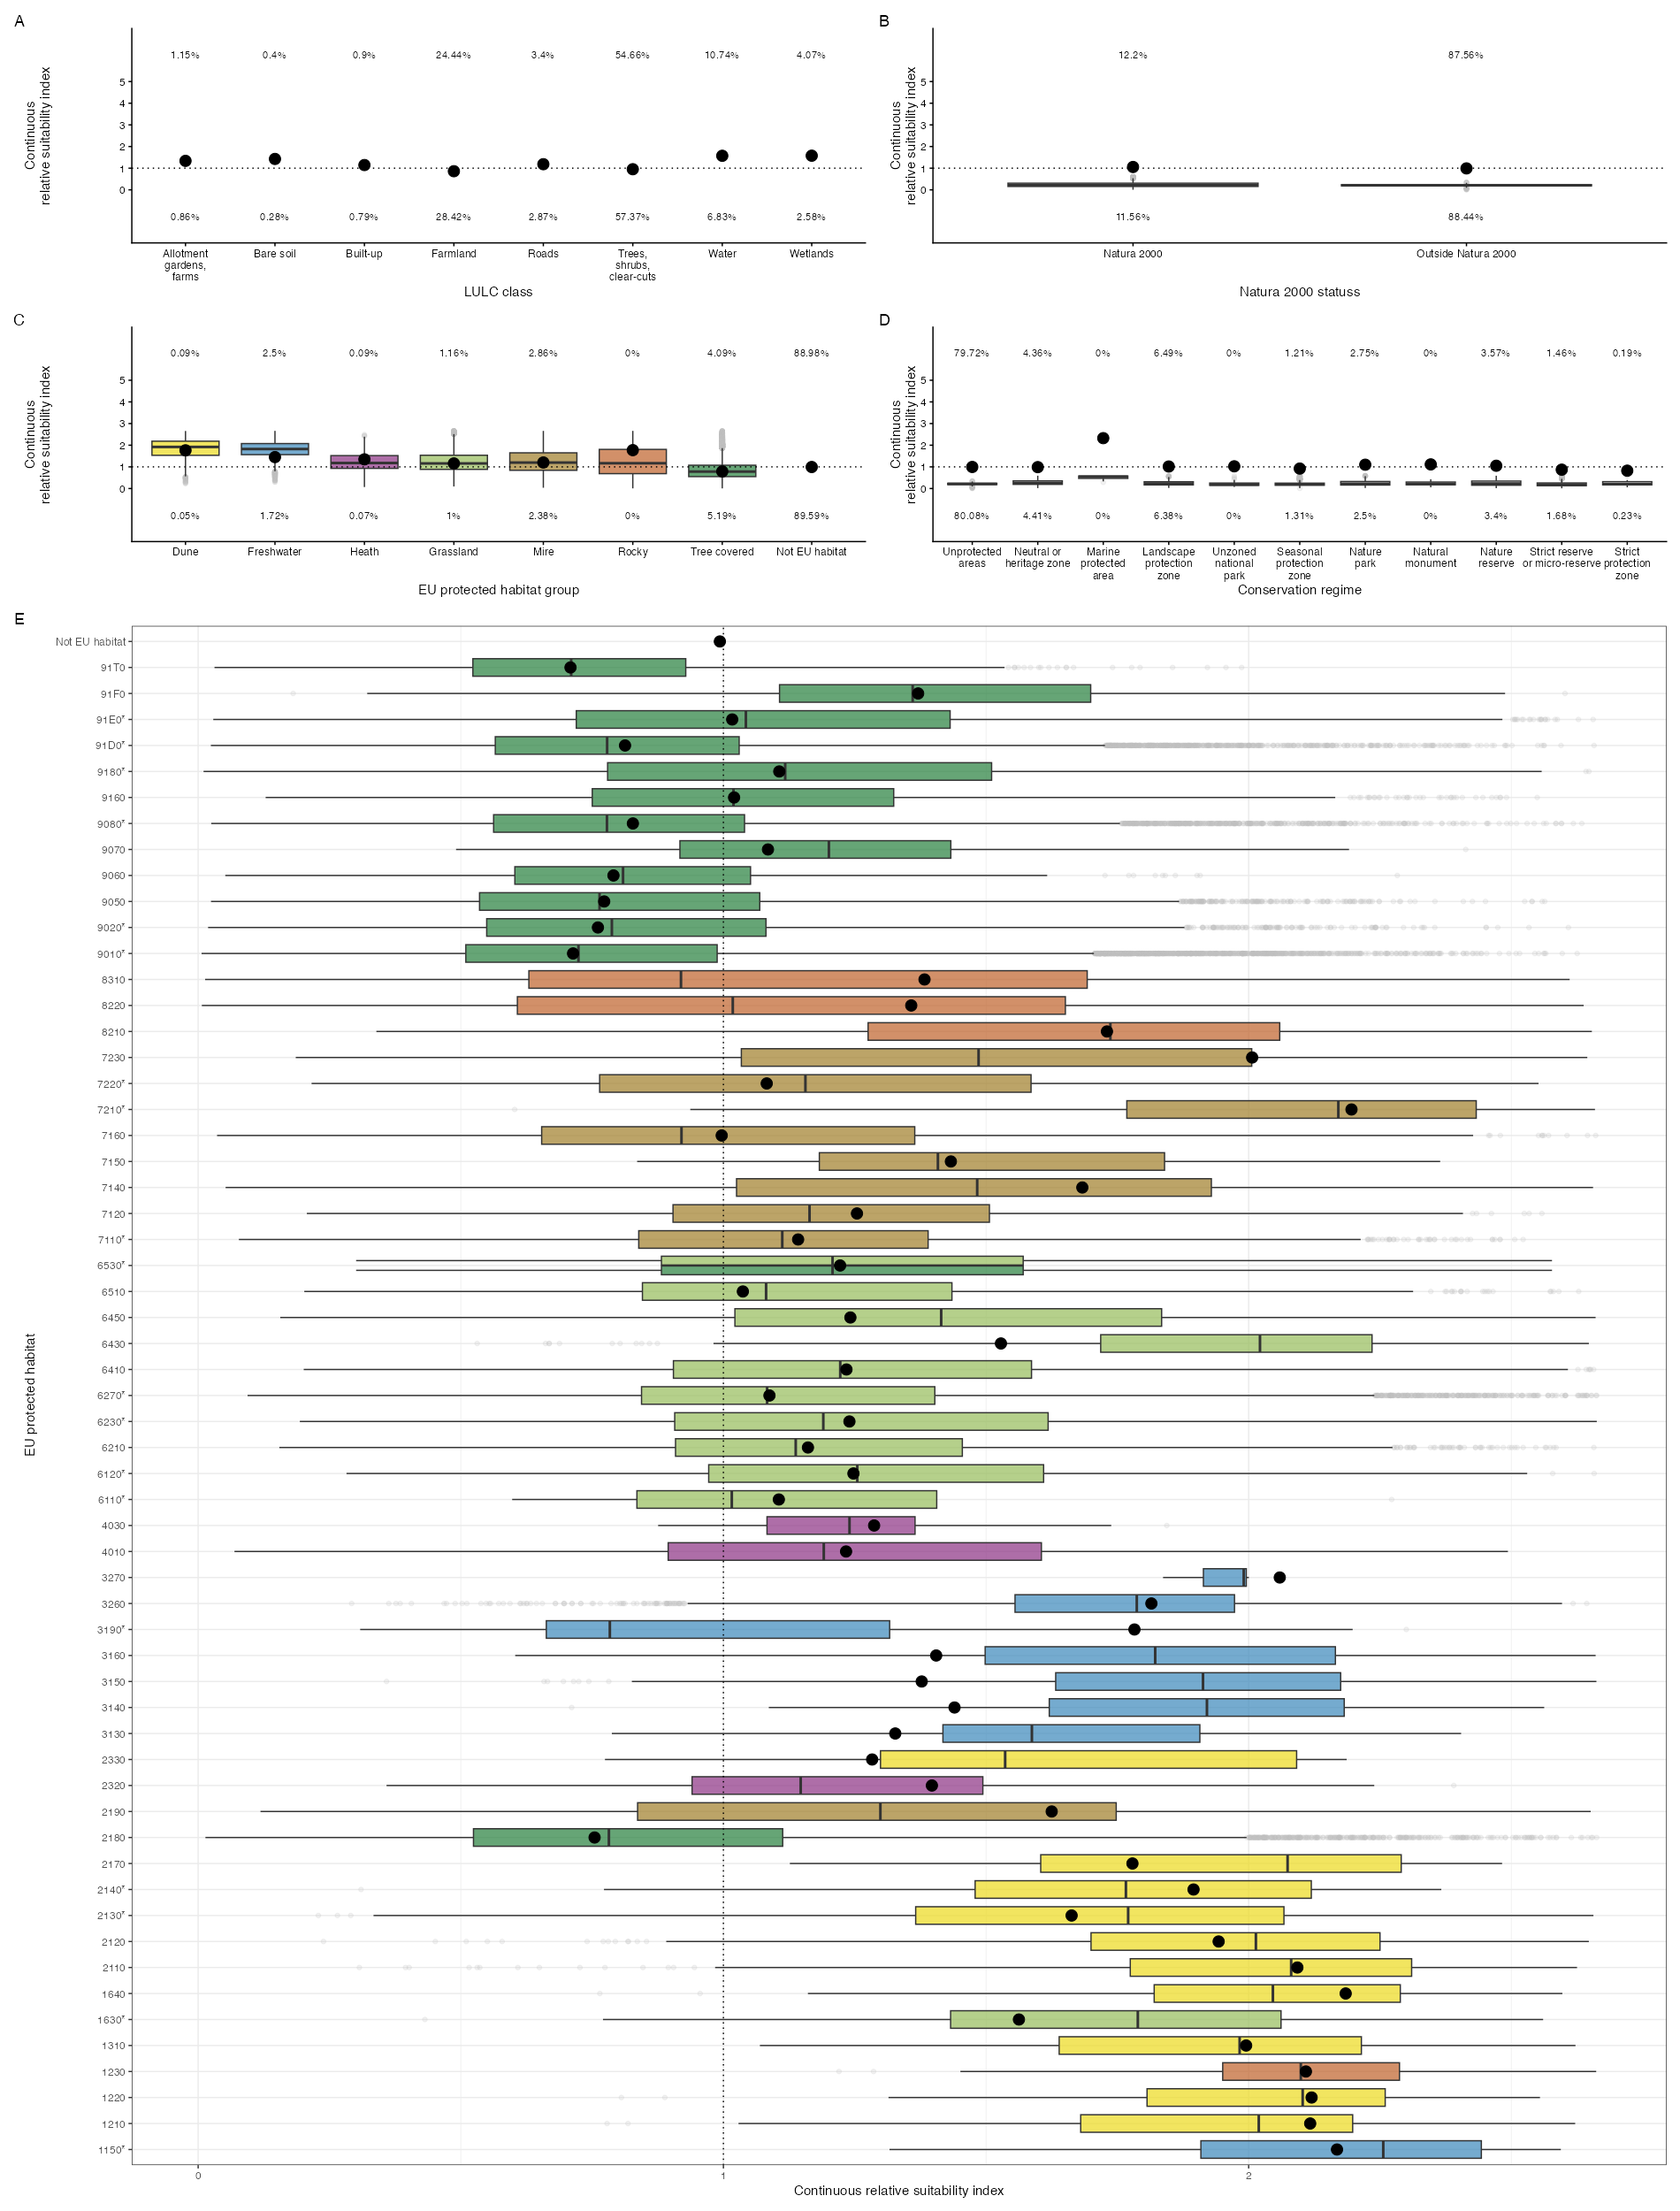
\includegraphics[width=1\linewidth,height=0.70\textheight,keepaspectratio]{results/RANARVv4a1/PicAssoc_RANARV.png}

\par\small\textit{Associations between predicted suitability and: (A) land use land cover classes, (B) Natura 2000 status, (C) stratified EU protected habitat classes, (D) conservation regime, and (E) EU protected habitats. The y-axis show continuous relative suitability index (derivative of Manly's index of preference). Colours in (C) and (E) correspond to stratified EU protected habitat classes. For classifications composed of multiple individual polygons, polygon-level indices were additionally calculated to show within-category variation. The figures therefore combine category-level estimates (points) with the distributions of polygon-level values (boxplots, where applicable). Labels above and below the panels report, respectively, the percentage of total predicted suitability and the percentage of mapped area represented by each category. **For a full resolution refer to repository: link or online document: link**}\normalsize
\end{center}

\section*{Conservation prioritization}\label{conservation-prioritization-18}
\addcontentsline{toc}{section}{Conservation prioritization}

\begin{center}
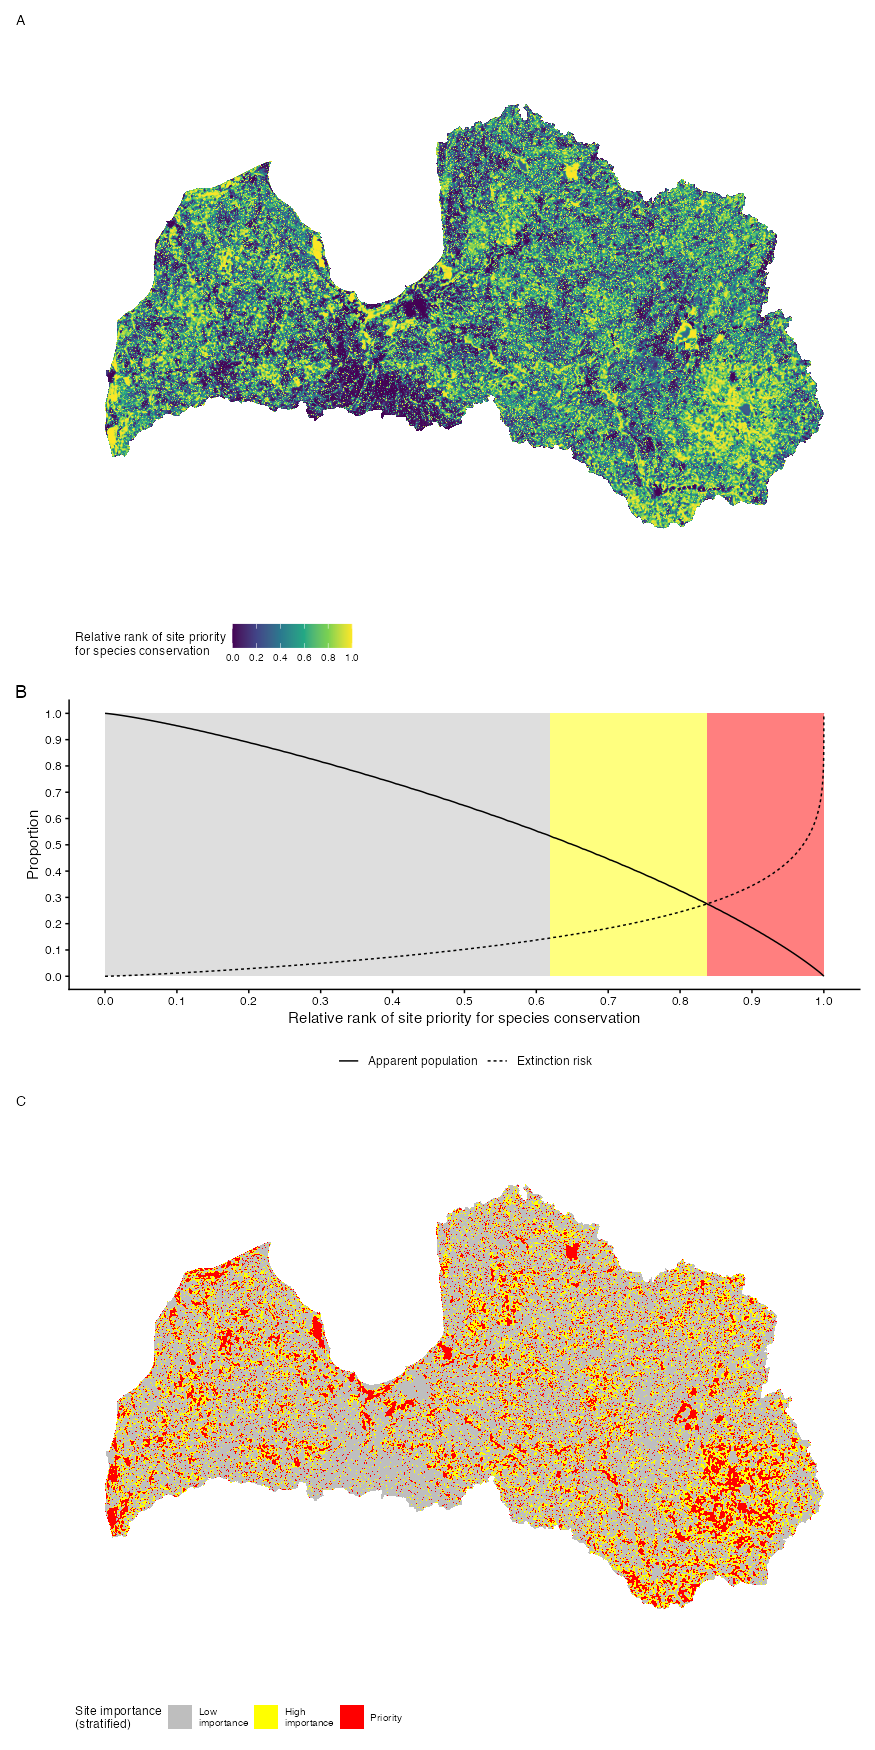
\includegraphics[width=0.85\linewidth,height=0.70\textheight,keepaspectratio]{results/RANARVv4a1/PicPrior_RANARV.png}

\par\small\textit{Single-species conservation prioritization focusing on maximisation of core area protection (CAZMAX) while accounting for site connectivity: (A) relative site rank; (B) relationship between apparent-population and extinction-risk curves with a simplified classification which is spatially demonstrated in the bootom row; (C) spatial distribution of proposed classification of site prioritization results. **For a full resolution refer to repository: link or online document: link**}\normalsize
\end{center}

\chapter*{\texorpdfstring{\emph{Rana arvalis} terrestrial}{Rana arvalis terrestrial}}\label{ranarvterrestrial}
\addcontentsline{toc}{chapter}{\emph{Rana arvalis} terrestrial}

\section*{Summary}\label{summary-19}
\addcontentsline{toc}{section}{Summary}

\subsection*{Model description}\label{model-description-19}
\addcontentsline{toc}{subsection}{Model description}

Occurrence and background data were divided into model-training with four block spatial cross-validation data and an independent test set. Sampling-bias/background treatment: \textbf{Phenology Weighted Target Group}. Accumulated LULC change within the 1-ha analysis cell was not evaluated; accumulated LULC change within the home-range radius around the analysis cell was not evaluated.

The final data set contained \textbf{160} presence records: \textbf{120} for training with four spatial block cross-validation and \textbf{40} for independent testing. Training background contained \textbf{30001} locations, with \textbf{9999} additional independent-test background locations.

\subsection*{Expert assessment scores}\label{expert-assessment-scores-19}
\addcontentsline{toc}{subsection}{Expert assessment scores}

\begin{itemize}
\tightlist
\item
  \textbf{Marginal responses and variable importance score:} 2 (limited ecological interpretability)
\item
  \textbf{Map score:} 3 (moderate agreement with known distribution)
\item
  \textbf{Applicability score:} 2 (limited applicability)
\end{itemize}

\textbf{Šo sadaļu aizpildām manuāli no ekspertu aptaujām}

\subsection*{Statistical evaluation}\label{statistical-evaluation-19}
\addcontentsline{toc}{subsection}{Statistical evaluation}

The final model had a training TSS of \textbf{0.401}, with a training-derived cloglog threshold of \textbf{0.345}. Combined training AUC was \textbf{0.846} and combined test AUC was \textbf{0.68}.

\subsubsection*{Spatial cross-validation}\label{spatial-cross-validation-19}
\addcontentsline{toc}{subsubsection}{Spatial cross-validation}

\begin{itemize}
\tightlist
\item
  \textbf{AUC:} 0.7845 ± 0.0514; null models: 0.508 ± 0.0357; z = 7.7385, p \textless{} 0.001
\item
  \textbf{CBI:} 0.7857 ± 0.0729; null models: -0.0174 ± 0.158; z = 5.0826, p \textless{} 0.001
\item
  \textbf{OR10:} 0.1833 ± 0.1291; null models: 0.2543 ± 0.072; z = -0.9863, p = 0.162
\item
  \textbf{ORmin:} 0.0583 ± 0.0687; null models: 0.0577 ± 0.0473; z = 0.0141, p = 0.506
\end{itemize}

\subsubsection*{Independent testing}\label{independent-testing-19}
\addcontentsline{toc}{subsubsection}{Independent testing}

\begin{itemize}
\tightlist
\item
  \textbf{TSS:} 0.176; \textbf{sensitivity:} 0.425; \textbf{specificity:} 0.751
\item
  \textbf{AUC:} 0.702; null models: 0.4963 ± 0.0741; z = 2.7699, p = 0.003
\item
  \textbf{CBI:} 0.528; null models: -0.0695 ± 0.4504; z = 1.3266, p = 0.092
\item
  \textbf{OR10:} 0.3; null models: 0.2205 ± 0.0966; z = 0.8234, p = 0.795
\item
  \textbf{ORmin:} 0.025; null models: 0.0245 ± 0.0326; z = 0.0154, p = 0.506
\end{itemize}

\subsection*{Conservation prioritisation summary}\label{conservation-prioritisation-summary-19}
\addcontentsline{toc}{subsection}{Conservation prioritisation summary}

The primary priority area covers \textbf{7.5\%} of Latvia and contains \textbf{27.5\%} of the summed habitat suitability (apparent population proxy).

The broader high importance area covers \textbf{27.5\%} of Latvia and contains \textbf{63.9\%} of the summed habitat suitability.

For comparison, the area classified as suitable using the maximum training sensitivity plus specificity habitat-suitability threshold contains \textbf{63.9\%} of the summed continuous habitat suitability.

\subsection*{Version evolution}\label{version-evolution-19}
\addcontentsline{toc}{subsection}{Version evolution}

\textbf{Šo sadaļu aizpildām manuāli, izmntojot sagatavotās shēmas. Jāvienojas par to noformējumu}

\section*{Habitat suitability}\label{habitat-suitability-19}
\addcontentsline{toc}{section}{Habitat suitability}

\begin{center}
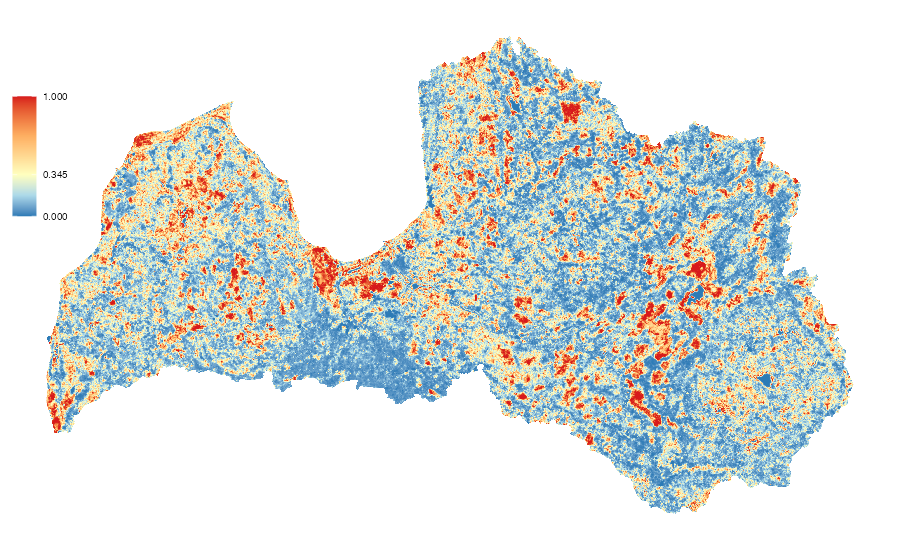
\includegraphics[width=1\linewidth,height=0.70\textheight,keepaspectratio]{results/RANARVterrestrialv2b1celi/PicHSmap_RANARVterrestrial.png}

\par\small\textit{Predicted continuous habitat suitability across Latvia. The warmer the colour the higher is the predicted habitat suitability. Value in the middle of the legend correspond to the maximum training sensitivity plus specificity threshold. **For a full resolution refer to repository: link or online document: link**}\normalsize
\end{center}

\section*{Model thresholds}\label{model-thresholds-19}
\addcontentsline{toc}{section}{Model thresholds}

Threshold values and associated omission rates

\begin{center}
\resizebox{\linewidth}{!}{%

\begin{tabular}{lrrrrr}
\toprule
Threshold & Cloglog value & Fractional predicted area & Training omission rate & Test omission rate & P-values\\
\midrule
Minimum training presence & 0.0571934 & 0.8062822 & 0.000 & 0.0000994 & 0\\
Equal training sensitivity and specificity & 0.3416966 & 0.2249958 & 0.225 & 0.0022867 & 0\\
Maximum training sensitivity plus specificity & 0.3448788 & 0.2225694 & 0.225 & 0.0022867 & 0\\
Equal test sensitivity and specificity & 0.2530641 & 0.3150740 & 0.150 & 0.0013919 & 0\\
Maximum test sensitivity plus specificity & 0.2408735 & 0.3315606 & 0.150 & 0.0012925 & 0\\
\bottomrule
\end{tabular}
}
\end{center}

\section*{Variable importance}\label{variable-importance-19}
\addcontentsline{toc}{section}{Variable importance}

\begin{center}
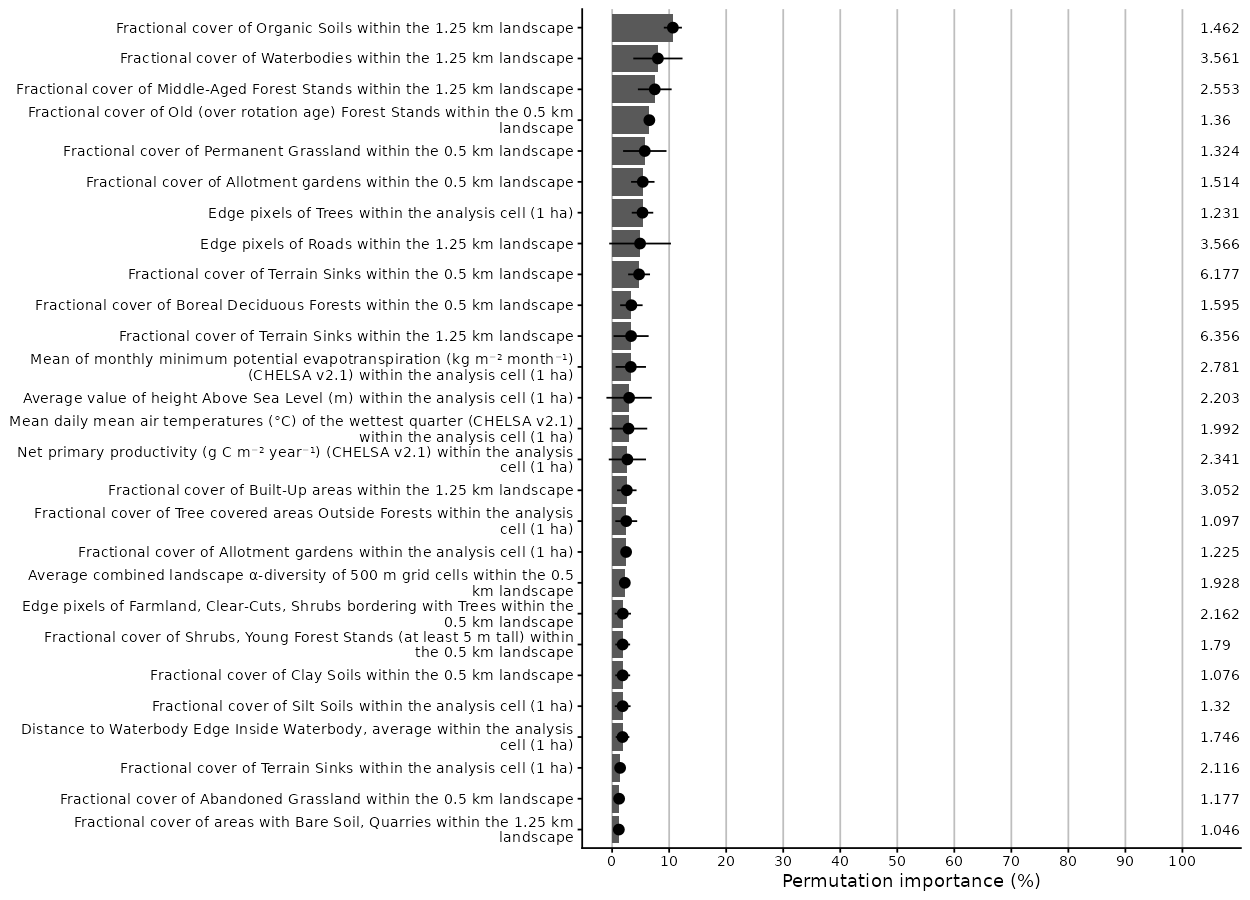
\includegraphics[width=1\linewidth,height=0.70\textheight,keepaspectratio]{results/RANARVterrestrialv2b1celi/PicVarImpVIFs_RANARVterrestrial.png}

\par\small\textit{Permutation-importance (mean and standard deviation from 99 permutations, on the x-axis) of the ecogeographical variables (first y-axis, left side), and their variance inflation factor values (second y-axis, right side). **For a full resolution refer to repository: link or online document: link**}\normalsize
\end{center}

\section*{Marginal responses}\label{marginal-responses-19}
\addcontentsline{toc}{section}{Marginal responses}

\begin{center}
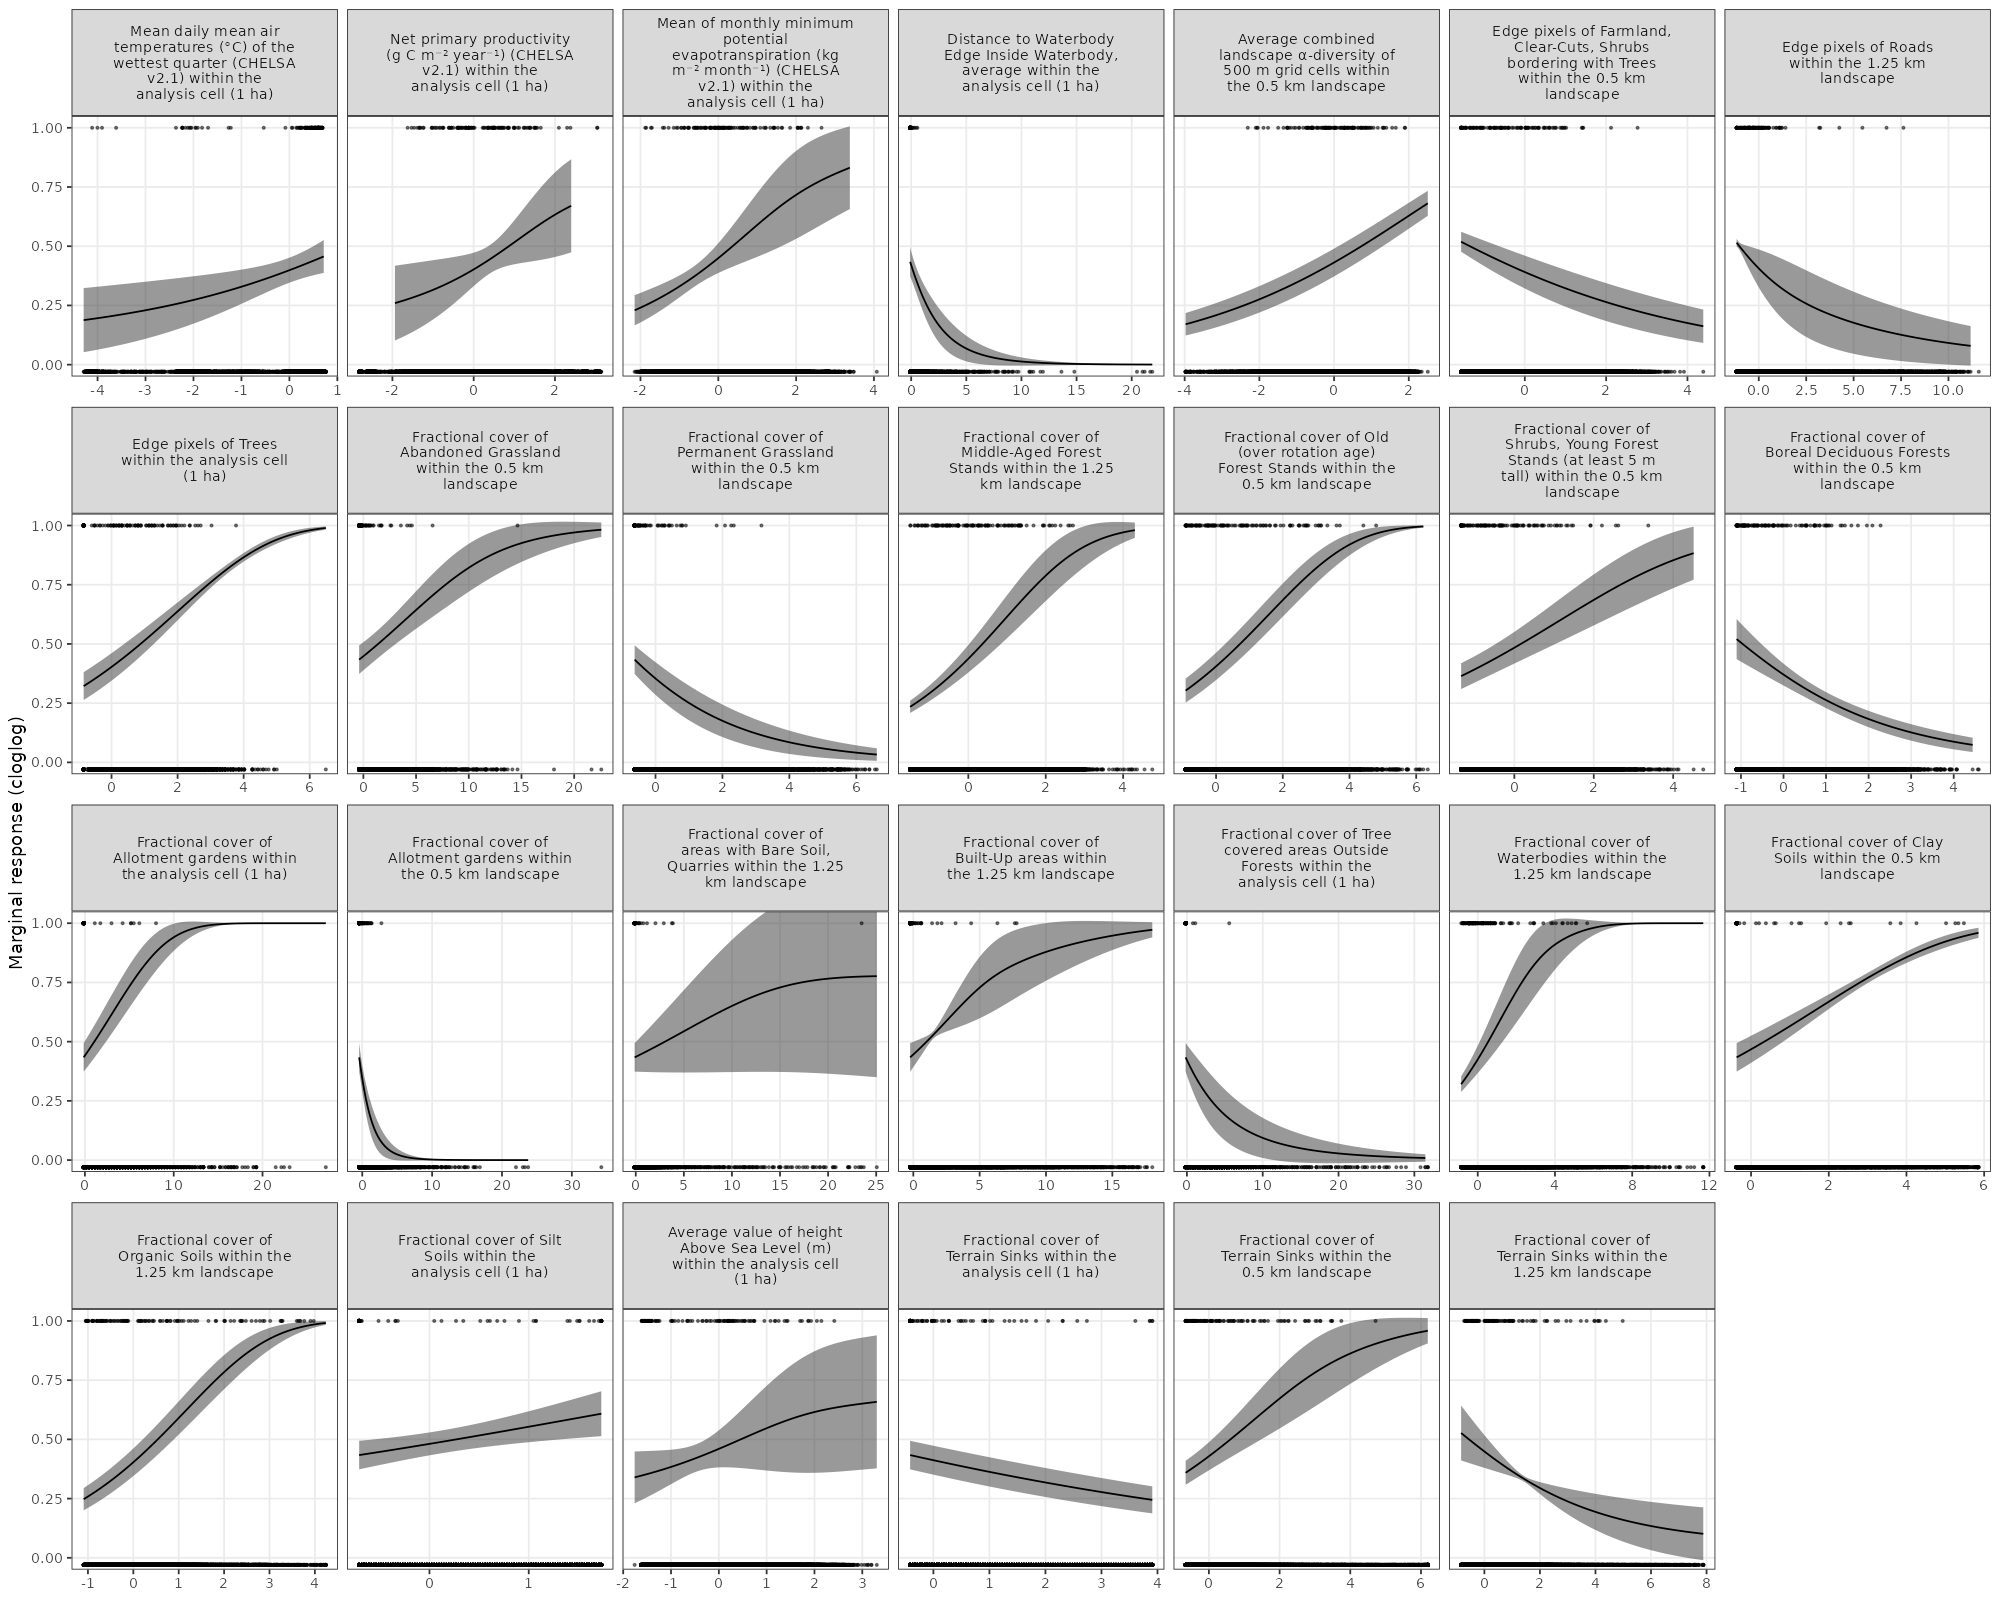
\includegraphics[width=1\linewidth,height=0.70\textheight,keepaspectratio]{results/RANARVterrestrialv2b1celi/PicMargResp_RANARVterrestrial.png}

\par\small\textit{Marginalised for arithmetic mean response curves illustrating the effect of each ecogeographical variable on the habitat suitability when all the other variables have their arithmetic mean values. The y-axis shows the predicted habitat suitability (cloglog-transformed), while the x-axis shows the standardised (centred and scaled) value of the ecogeographical variable. Dots at a value of 1 on the y-axis illustrate presence locations in the environment (on the x-axis), while dots at a value of 0 illustrate background locations used in modelling.  **For a full resolution refer to repository: link or online document: link**}\normalsize
\end{center}

\section*{Habitat and conservation associations}\label{habitat-and-conservation-associations-19}
\addcontentsline{toc}{section}{Habitat and conservation associations}

\begin{center}
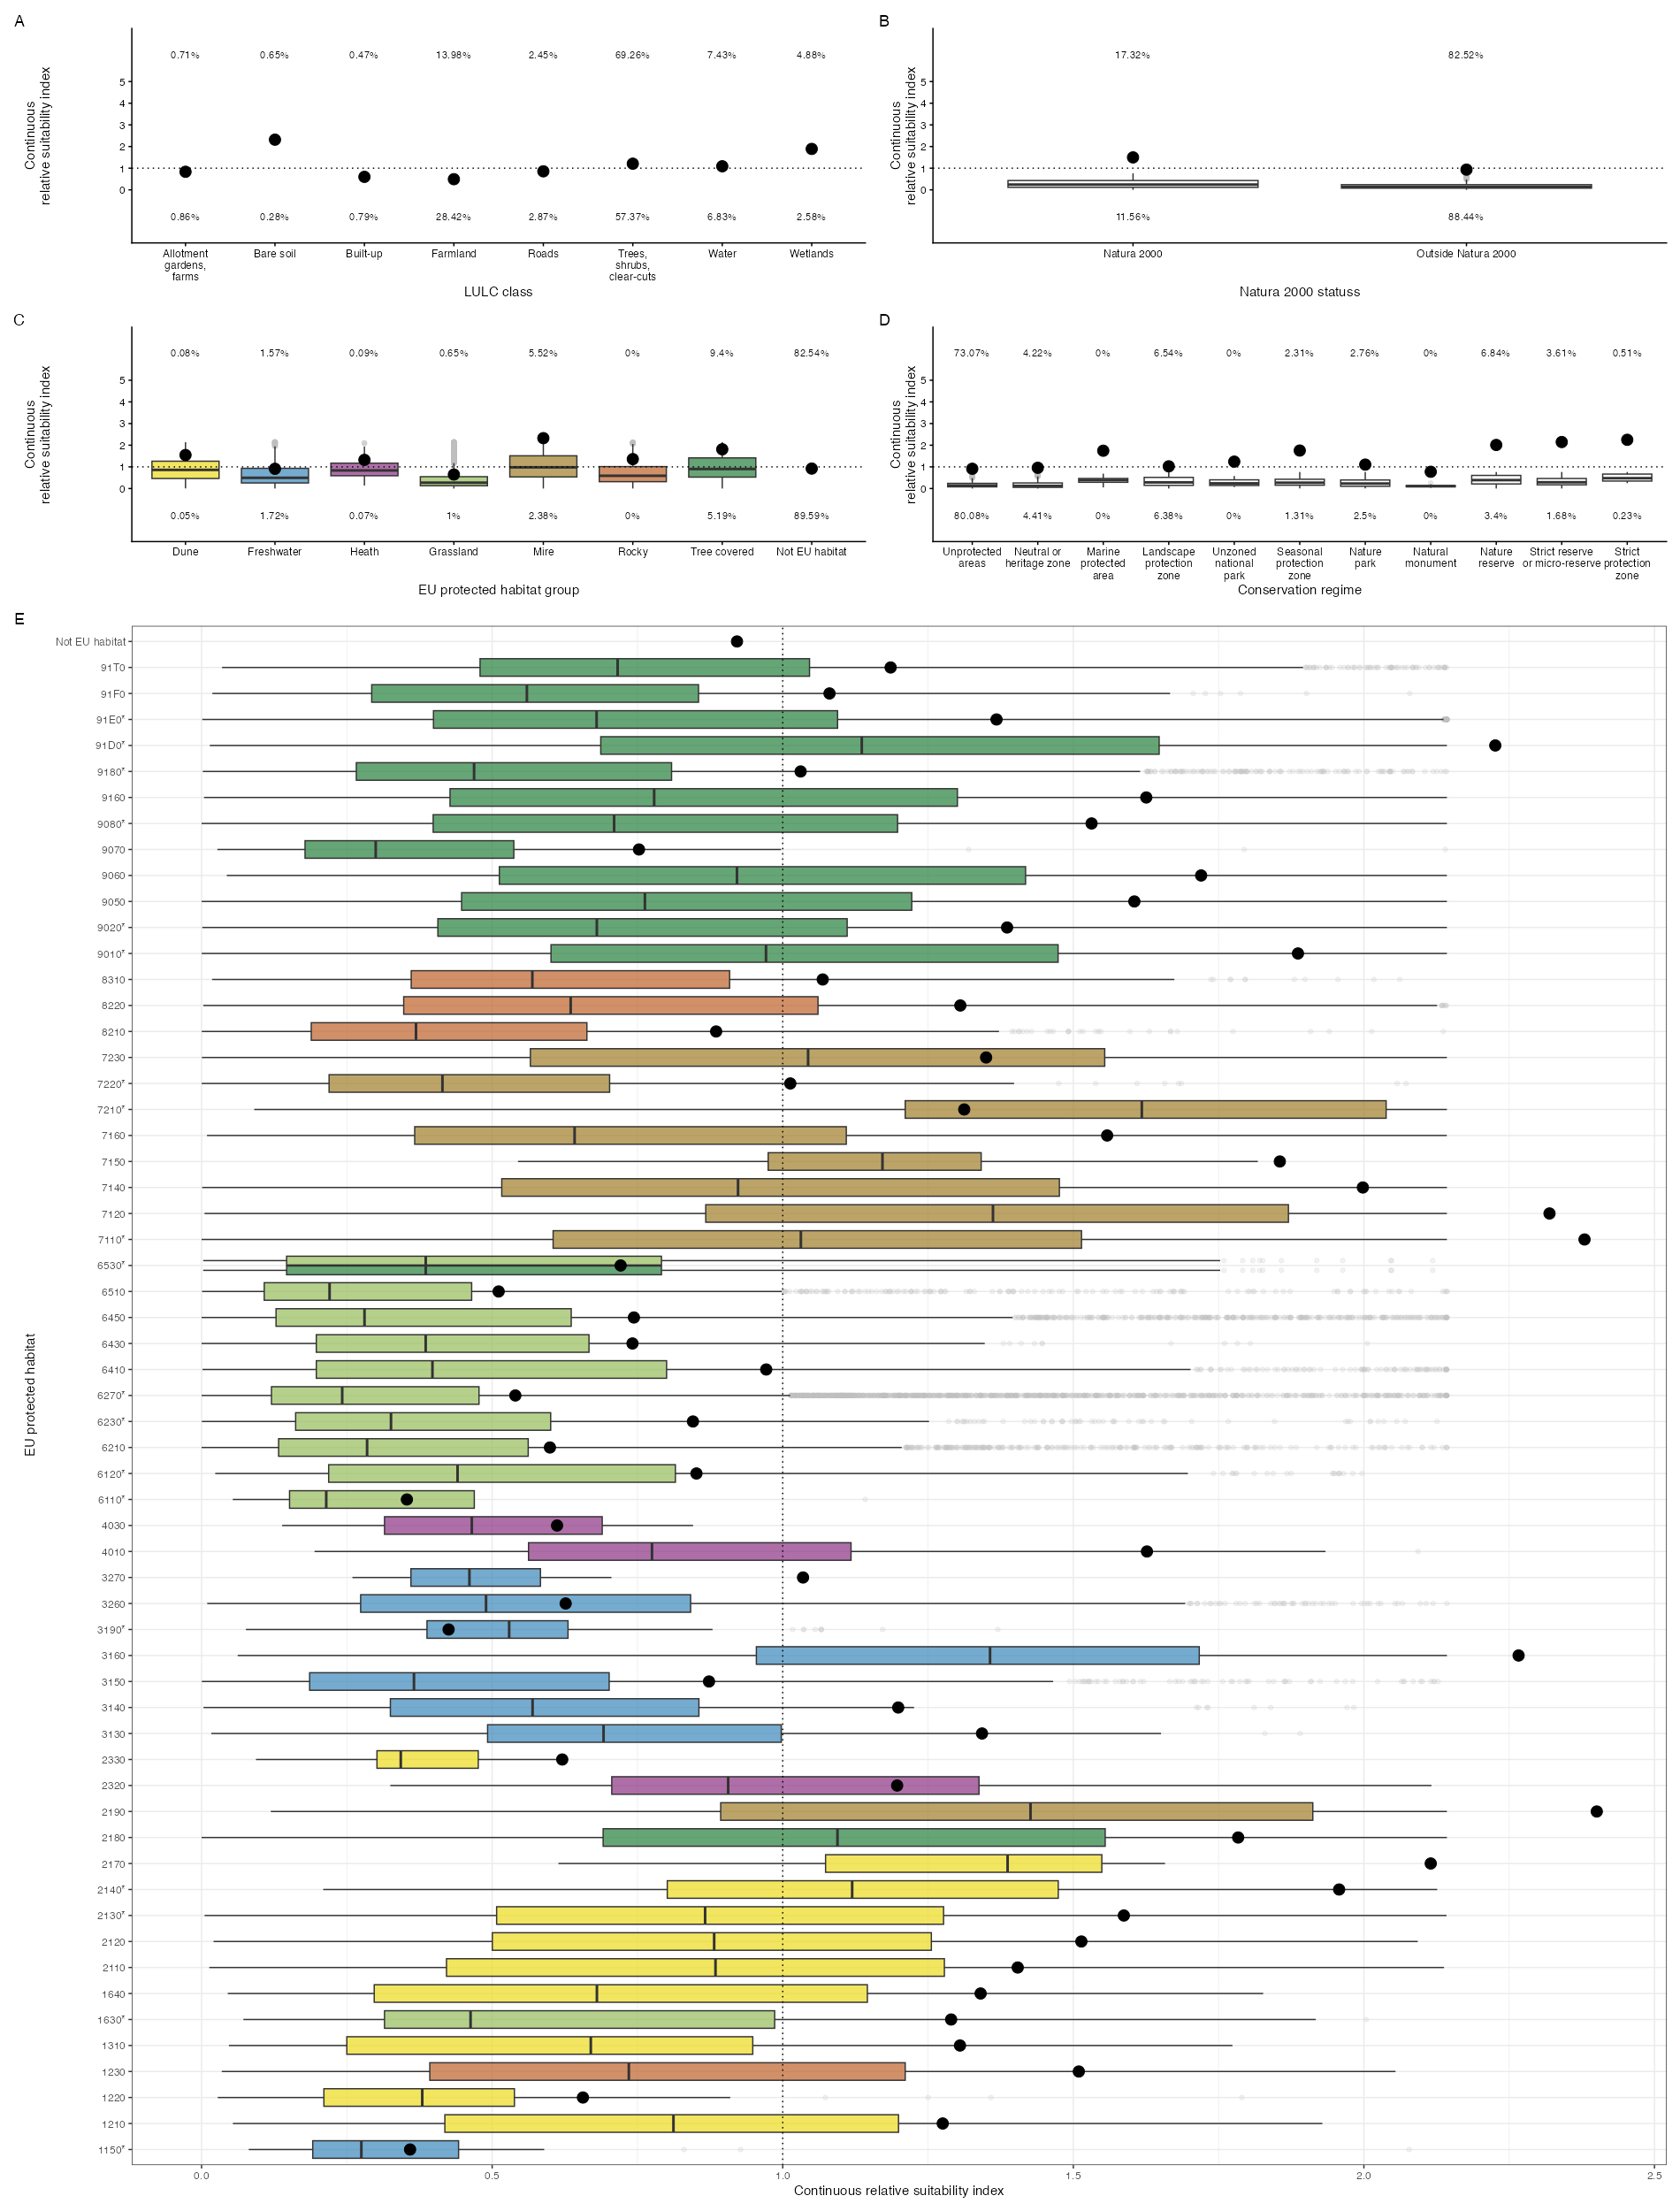
\includegraphics[width=1\linewidth,height=0.70\textheight,keepaspectratio]{results/RANARVterrestrialv2b1celi/PicAssoc_RANARVterrestrial.png}

\par\small\textit{Associations between predicted suitability and: (A) land use land cover classes, (B) Natura 2000 status, (C) stratified EU protected habitat classes, (D) conservation regime, and (E) EU protected habitats. The y-axis show continuous relative suitability index (derivative of Manly's index of preference). Colours in (C) and (E) correspond to stratified EU protected habitat classes. For classifications composed of multiple individual polygons, polygon-level indices were additionally calculated to show within-category variation. The figures therefore combine category-level estimates (points) with the distributions of polygon-level values (boxplots, where applicable). Labels above and below the panels report, respectively, the percentage of total predicted suitability and the percentage of mapped area represented by each category. **For a full resolution refer to repository: link or online document: link**}\normalsize
\end{center}

\section*{Conservation prioritization}\label{conservation-prioritization-19}
\addcontentsline{toc}{section}{Conservation prioritization}

\begin{center}
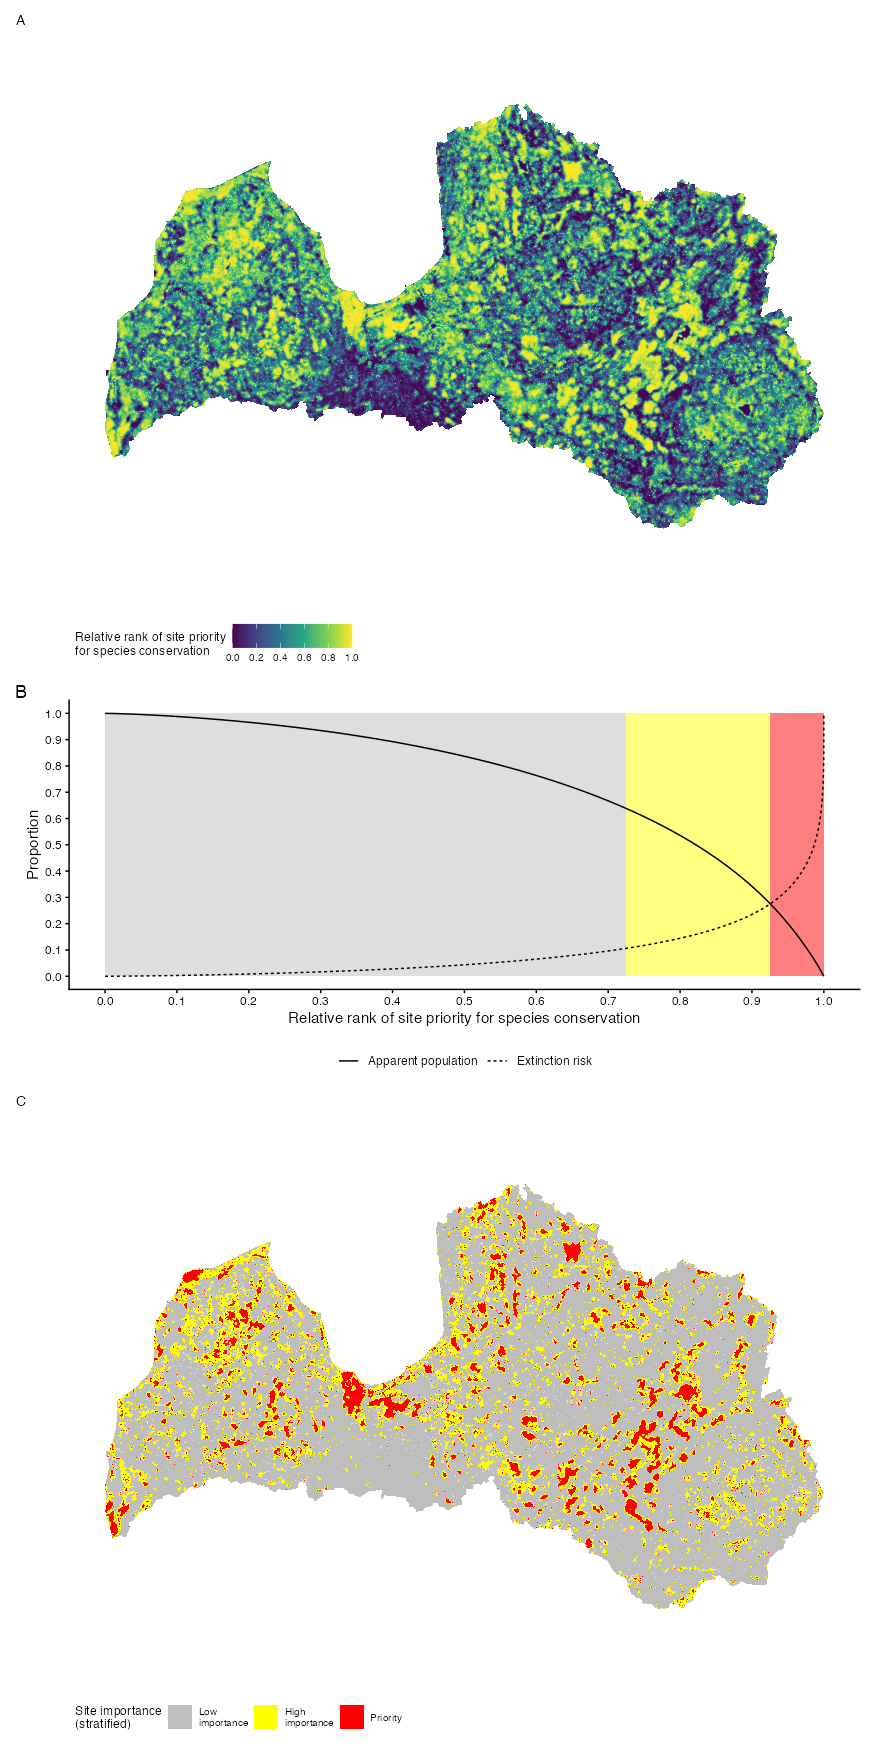
\includegraphics[width=0.85\linewidth,height=0.70\textheight,keepaspectratio]{results/RANARVterrestrialv2b1celi/PicPrior_RANARVterrestrial.png}

\par\small\textit{Single-species conservation prioritization focusing on maximisation of core area protection (CAZMAX) while accounting for site connectivity: (A) relative site rank; (B) relationship between apparent-population and extinction-risk curves with a simplified classification which is spatially demonstrated in the bootom row; (C) spatial distribution of proposed classification of site prioritization results. **For a full resolution refer to repository: link or online document: link**}\normalsize
\end{center}

\chapter*{\texorpdfstring{\emph{Rana arvalis} monitoring}{Rana arvalis monitoring}}\label{ranarvmonitoring}
\addcontentsline{toc}{chapter}{\emph{Rana arvalis} monitoring}

\section*{Summary}\label{summary-20}
\addcontentsline{toc}{section}{Summary}

\subsection*{Model description}\label{model-description-20}
\addcontentsline{toc}{subsection}{Model description}

Occurrence and background data were divided into model-training with four block spatial cross-validation data and an independent test set. Sampling-bias/background treatment: \textbf{Phenology Weighted Target Group}. Accumulated LULC change within the 1-ha analysis cell was not evaluated; accumulated LULC change within the home-range radius around the analysis cell was not evaluated.

The final data set contained \textbf{707} presence records: \textbf{530} for training with four spatial block cross-validation and \textbf{177} for independent testing. Training background contained \textbf{29986} locations, with \textbf{10014} additional independent-test background locations.

\subsection*{Expert assessment scores}\label{expert-assessment-scores-20}
\addcontentsline{toc}{subsection}{Expert assessment scores}

\begin{itemize}
\tightlist
\item
  \textbf{Marginal responses and variable importance score:} 2 (limited ecological interpretability)
\item
  \textbf{Map score:} 2 (limited agreement with known distribution)
\item
  \textbf{Applicability score:} 2 (limited applicability)
\end{itemize}

\textbf{Šo sadaļu aizpildām manuāli no ekspertu aptaujām}

\subsection*{Statistical evaluation}\label{statistical-evaluation-20}
\addcontentsline{toc}{subsection}{Statistical evaluation}

The final model had a training TSS of \textbf{0.401}, with a training-derived cloglog threshold of \textbf{0.562}. Combined training AUC was \textbf{0.786} and combined test AUC was \textbf{0.756}.

\subsubsection*{Spatial cross-validation}\label{spatial-cross-validation-20}
\addcontentsline{toc}{subsubsection}{Spatial cross-validation}

\begin{itemize}
\tightlist
\item
  \textbf{AUC:} 0.785 ± 0.019; null models: 0.5198 ± 0.0193; z = 13.7159, p \textless{} 0.001
\item
  \textbf{CBI:} 0.949 ± 0.034; null models: 0.1286 ± 0.1664; z = 4.9296, p \textless{} 0.001
\item
  \textbf{OR10:} 0.1095 ± 0.0779; null models: 0.0365 ± 0.028; z = 2.6118, p = 0.995
\item
  \textbf{ORmin:} 0.0038 ± 0.0075; null models: 2e-04 ± 0.0013; z = 2.7977, p = 0.997
\end{itemize}

\subsubsection*{Independent testing}\label{independent-testing-20}
\addcontentsline{toc}{subsubsection}{Independent testing}

\begin{itemize}
\tightlist
\item
  \textbf{TSS:} 0.416; \textbf{sensitivity:} 0.746; \textbf{specificity:} 0.671
\item
  \textbf{AUC:} 0.735; null models: 0.516 ± 0.0535; z = 4.0923, p \textless{} 0.001
\item
  \textbf{CBI:} 0.946; null models: 0.1532 ± 0.4287; z = 1.8496, p = 0.032
\item
  \textbf{OR10:} 0.175; null models: 0.0395 ± 0.0435; z = 3.1205, p = 0.999
\item
  \textbf{ORmin:} 0.017; null models: 2e-04 ± 0.0013; z = 13.3362, p = 1
\end{itemize}

\subsection*{Conservation prioritisation summary}\label{conservation-prioritisation-summary-20}
\addcontentsline{toc}{subsection}{Conservation prioritisation summary}

The primary priority area covers \textbf{15.9\%} of Latvia and contains \textbf{27.6\%} of the summed habitat suitability (apparent population proxy).

The broader high importance area covers \textbf{29.9\%} of Latvia and contains \textbf{46.5\%} of the summed habitat suitability.

For comparison, the area classified as suitable using the maximum training sensitivity plus specificity habitat-suitability threshold contains \textbf{46.5\%} of the summed continuous habitat suitability.

\subsection*{Version evolution}\label{version-evolution-20}
\addcontentsline{toc}{subsection}{Version evolution}

\textbf{Šo sadaļu aizpildām manuāli, izmntojot sagatavotās shēmas. Jāvienojas par to noformējumu}

\section*{Habitat suitability}\label{habitat-suitability-20}
\addcontentsline{toc}{section}{Habitat suitability}

\begin{center}
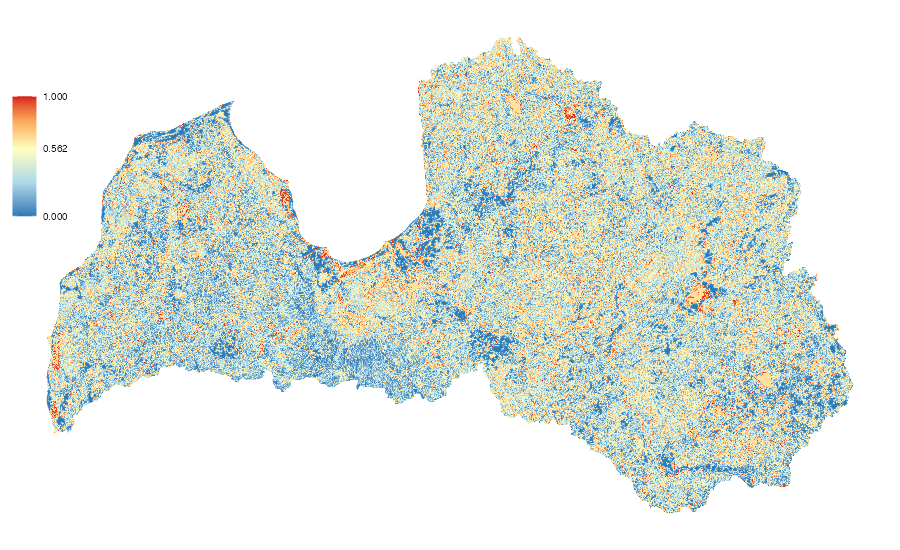
\includegraphics[width=1\linewidth,height=0.70\textheight,keepaspectratio]{results/RANARVmonitoringv2b5celi/PicHSmap_RANARVmonitoring.png}

\par\small\textit{Predicted continuous habitat suitability across Latvia. The warmer the colour the higher is the predicted habitat suitability. Value in the middle of the legend correspond to the maximum training sensitivity plus specificity threshold. **For a full resolution refer to repository: link or online document: link**}\normalsize
\end{center}

\section*{Model thresholds}\label{model-thresholds-20}
\addcontentsline{toc}{section}{Model thresholds}

Threshold values and associated omission rates

\begin{center}
\resizebox{\linewidth}{!}{%

\begin{tabular}{lrrrrr}
\toprule
Threshold & Cloglog value & Fractional predicted area & Training omission rate & Test omission rate & P-values\\
\midrule
Minimum training presence & 0.0587234 & 0.9722231 & 0.0000000 & 0.0002921 & 0\\
Equal training sensitivity and specificity & 0.6178316 & 0.2770080 & 0.2773585 & 0.0063279 & 0\\
Maximum training sensitivity plus specificity & 0.5617737 & 0.3561059 & 0.1867925 & 0.0043808 & 0\\
Equal test sensitivity and specificity & 0.5834817 & 0.3254522 & 0.2283019 & 0.0051597 & 0\\
Maximum test sensitivity plus specificity & 0.5623181 & 0.3553454 & 0.1886792 & 0.0043808 & 0\\
\bottomrule
\end{tabular}
}
\end{center}

\section*{Variable importance}\label{variable-importance-20}
\addcontentsline{toc}{section}{Variable importance}

\begin{center}
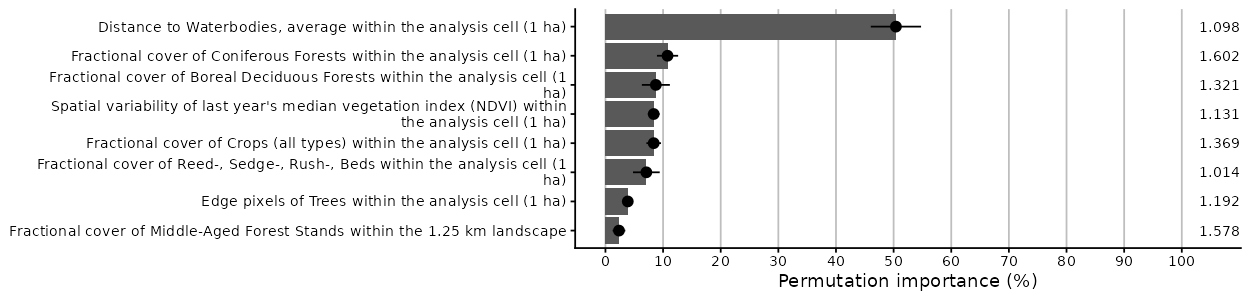
\includegraphics[width=1\linewidth,height=0.70\textheight,keepaspectratio]{results/RANARVmonitoringv2b5celi/PicVarImpVIFs_RANARVmonitoring.png}

\par\small\textit{Permutation-importance (mean and standard deviation from 99 permutations, on the x-axis) of the ecogeographical variables (first y-axis, left side), and their variance inflation factor values (second y-axis, right side). **For a full resolution refer to repository: link or online document: link**}\normalsize
\end{center}

\section*{Marginal responses}\label{marginal-responses-20}
\addcontentsline{toc}{section}{Marginal responses}

\begin{center}
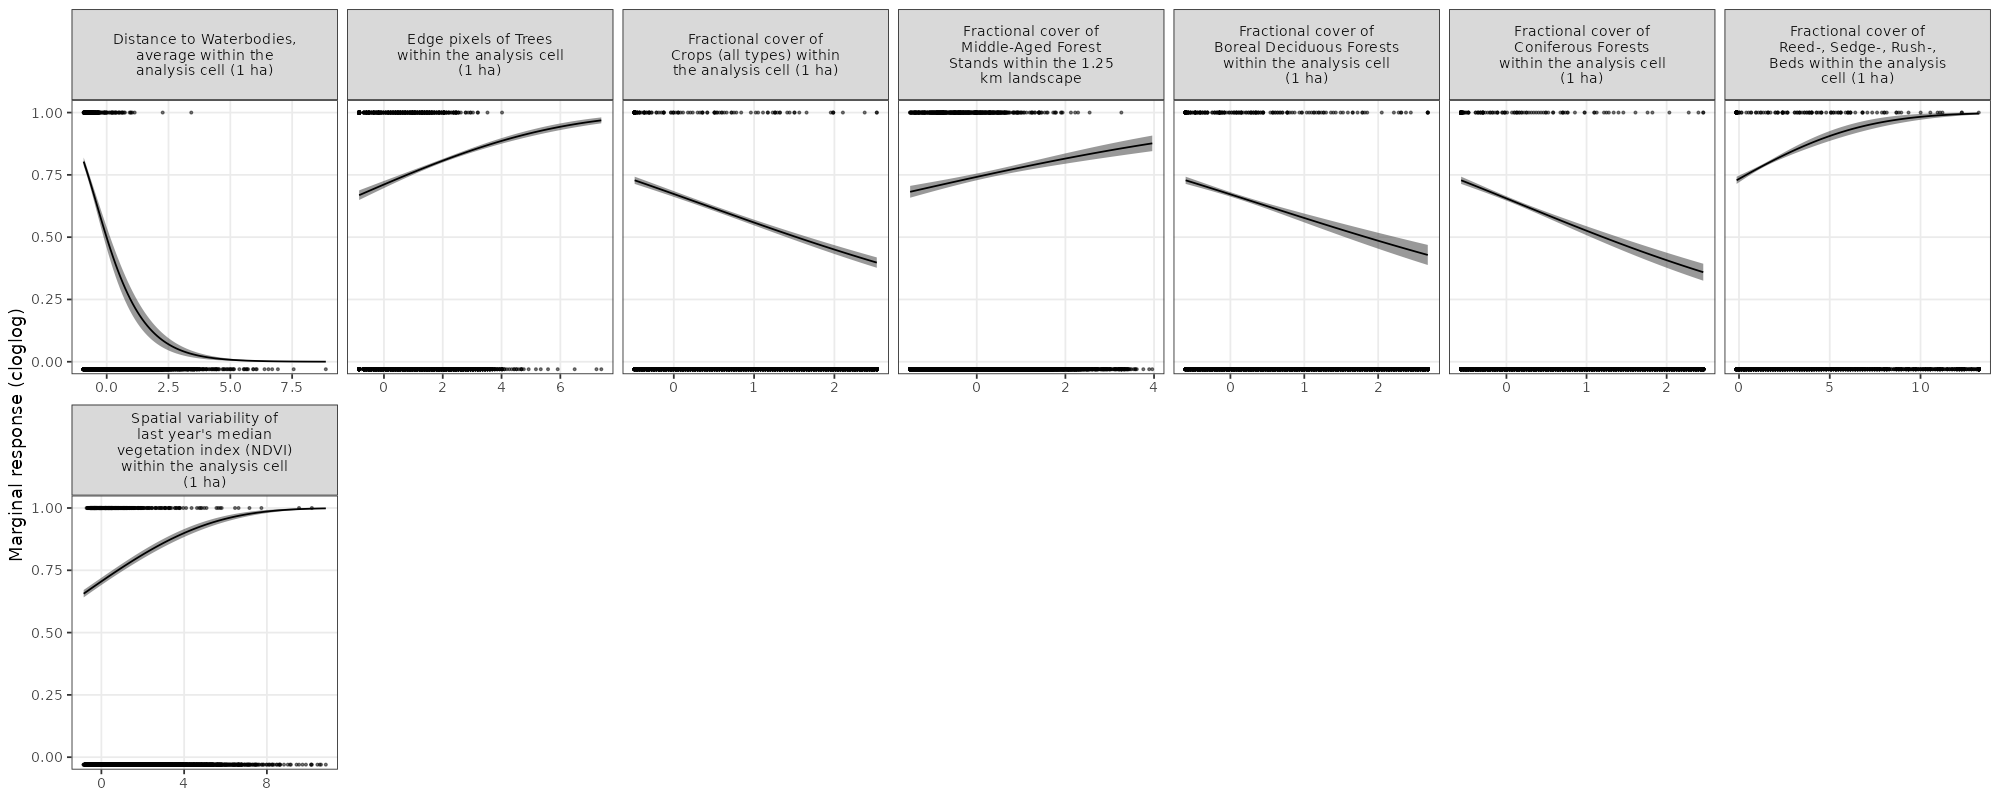
\includegraphics[width=1\linewidth,height=0.70\textheight,keepaspectratio]{results/RANARVmonitoringv2b5celi/PicMargResp_RANARVmonitoring.png}

\par\small\textit{Marginalised for arithmetic mean response curves illustrating the effect of each ecogeographical variable on the habitat suitability when all the other variables have their arithmetic mean values. The y-axis shows the predicted habitat suitability (cloglog-transformed), while the x-axis shows the standardised (centred and scaled) value of the ecogeographical variable. Dots at a value of 1 on the y-axis illustrate presence locations in the environment (on the x-axis), while dots at a value of 0 illustrate background locations used in modelling.  **For a full resolution refer to repository: link or online document: link**}\normalsize
\end{center}

\section*{Habitat and conservation associations}\label{habitat-and-conservation-associations-20}
\addcontentsline{toc}{section}{Habitat and conservation associations}

\begin{center}
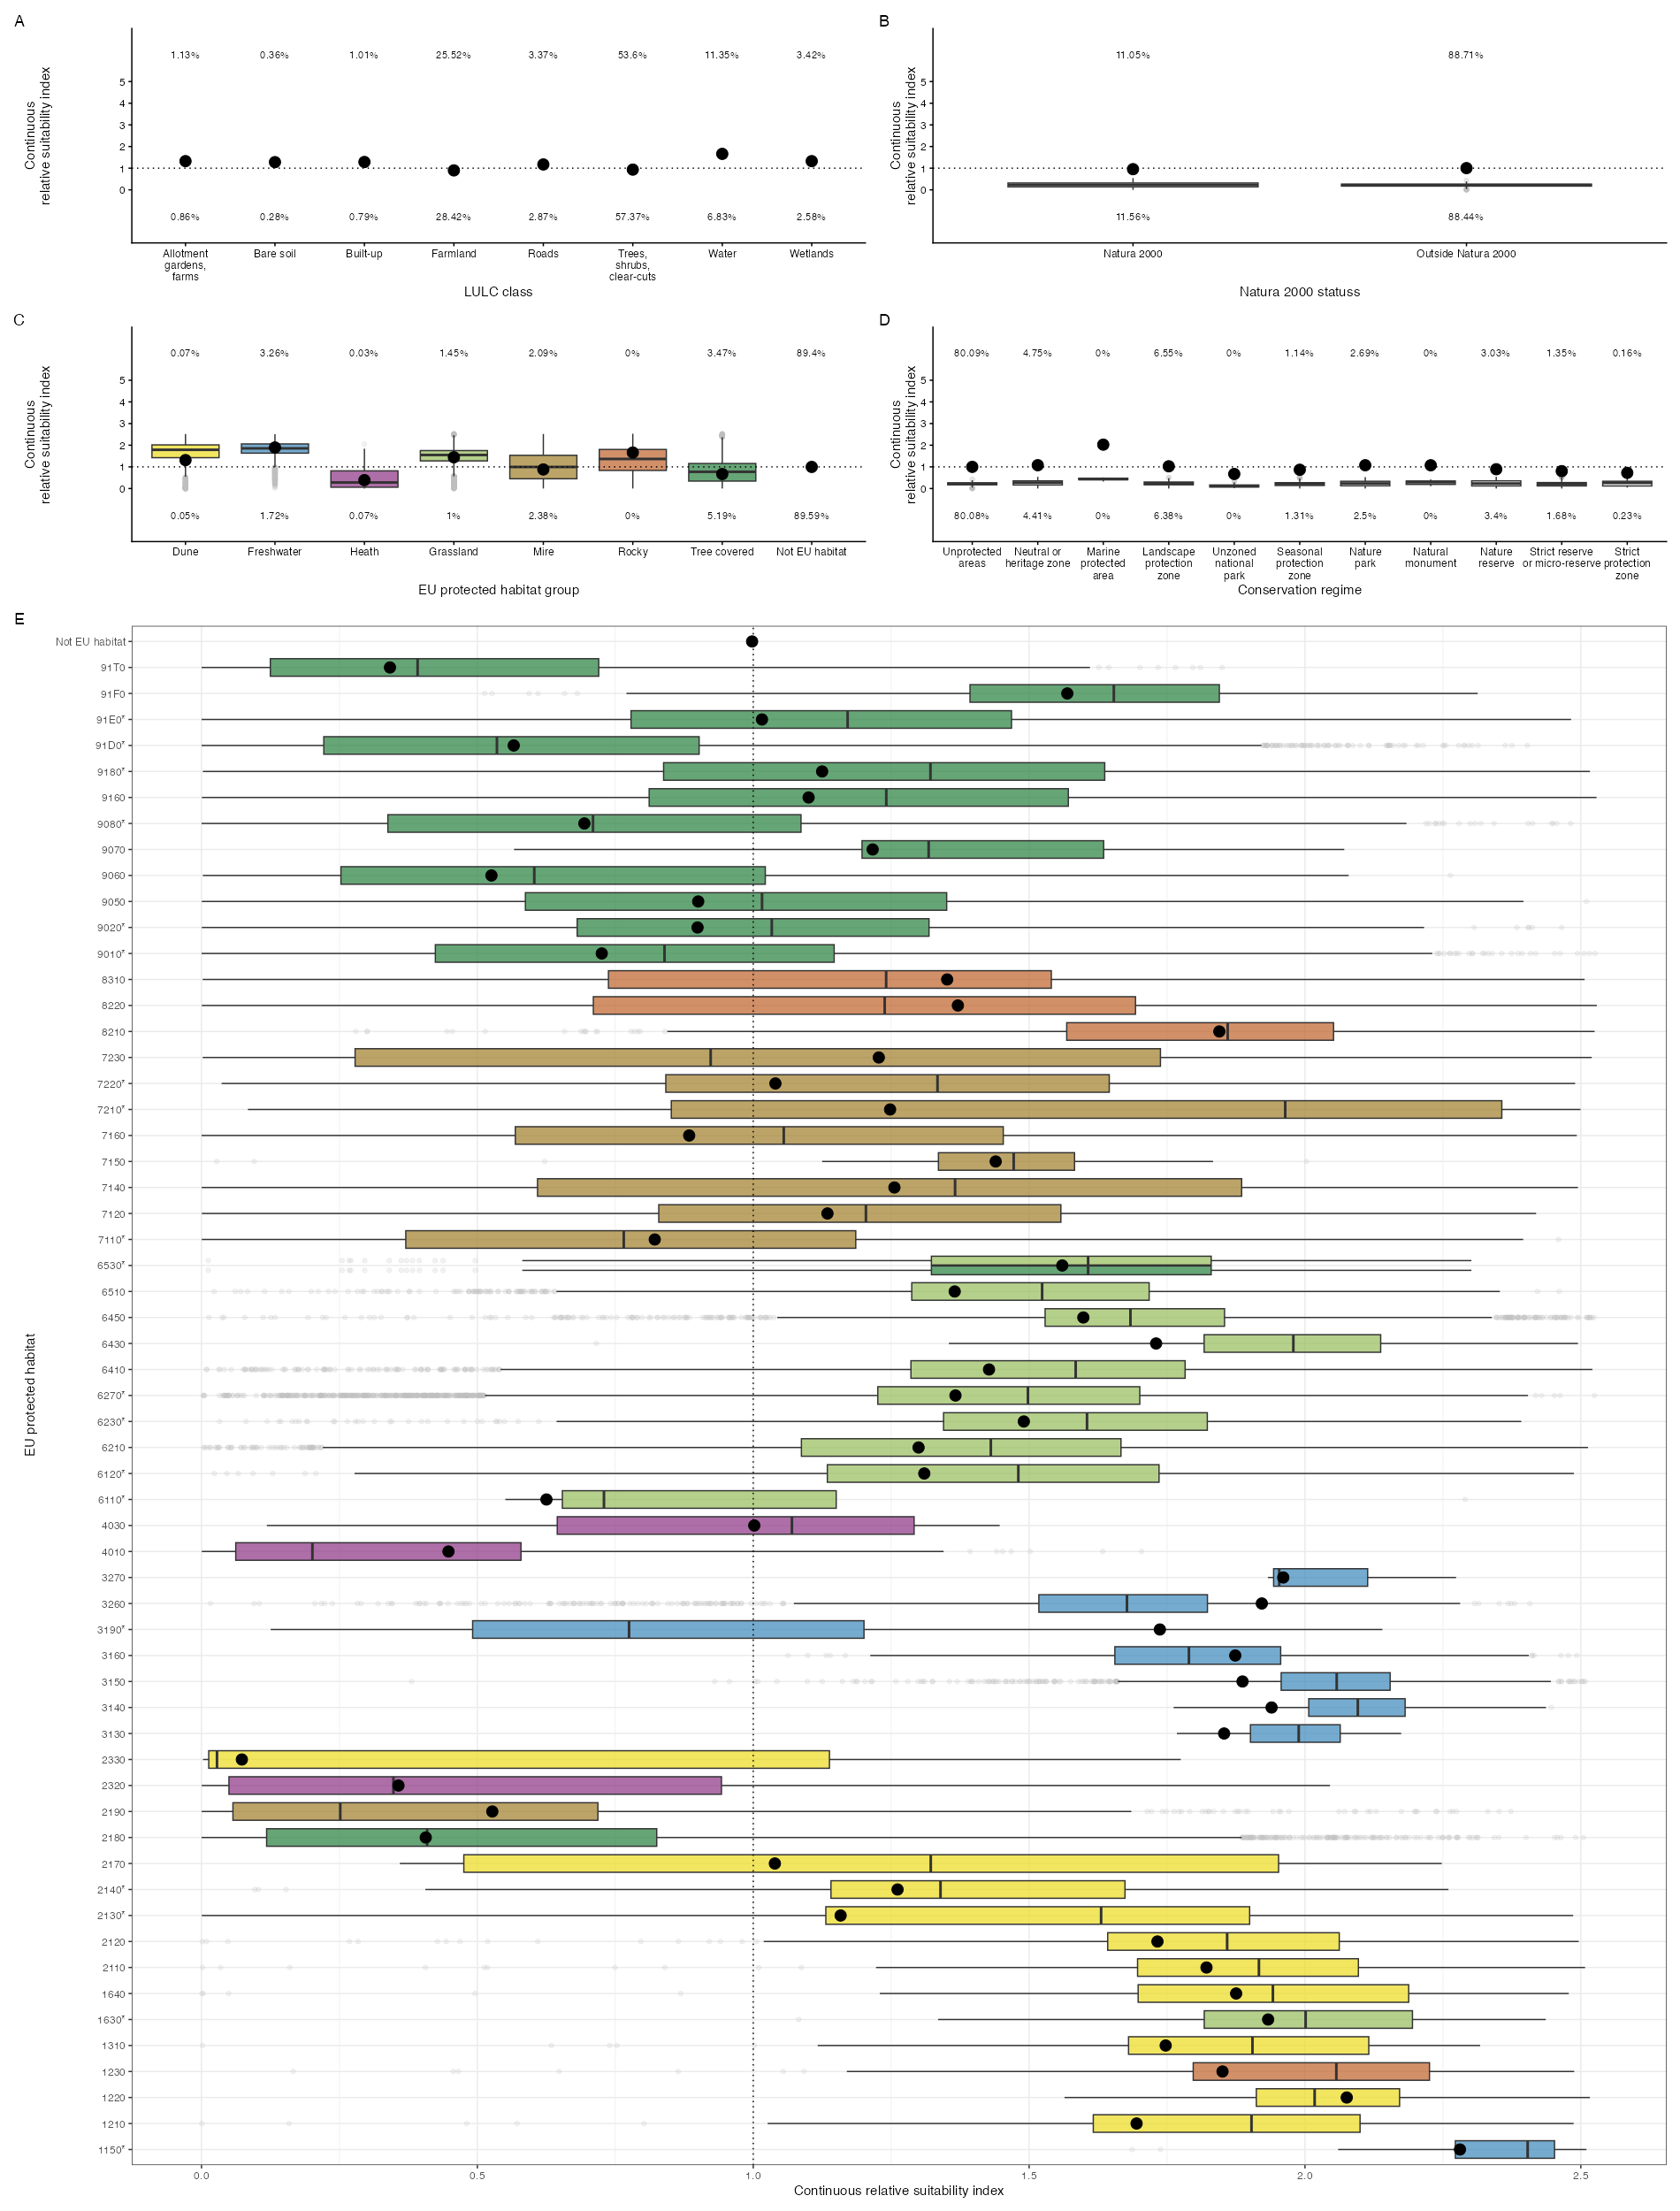
\includegraphics[width=1\linewidth,height=0.70\textheight,keepaspectratio]{results/RANARVmonitoringv2b5celi/PicAssoc_RANARVmonitoring.png}

\par\small\textit{Associations between predicted suitability and: (A) land use land cover classes, (B) Natura 2000 status, (C) stratified EU protected habitat classes, (D) conservation regime, and (E) EU protected habitats. The y-axis show continuous relative suitability index (derivative of Manly's index of preference). Colours in (C) and (E) correspond to stratified EU protected habitat classes. For classifications composed of multiple individual polygons, polygon-level indices were additionally calculated to show within-category variation. The figures therefore combine category-level estimates (points) with the distributions of polygon-level values (boxplots, where applicable). Labels above and below the panels report, respectively, the percentage of total predicted suitability and the percentage of mapped area represented by each category. **For a full resolution refer to repository: link or online document: link**}\normalsize
\end{center}

\section*{Conservation prioritization}\label{conservation-prioritization-20}
\addcontentsline{toc}{section}{Conservation prioritization}

\begin{center}
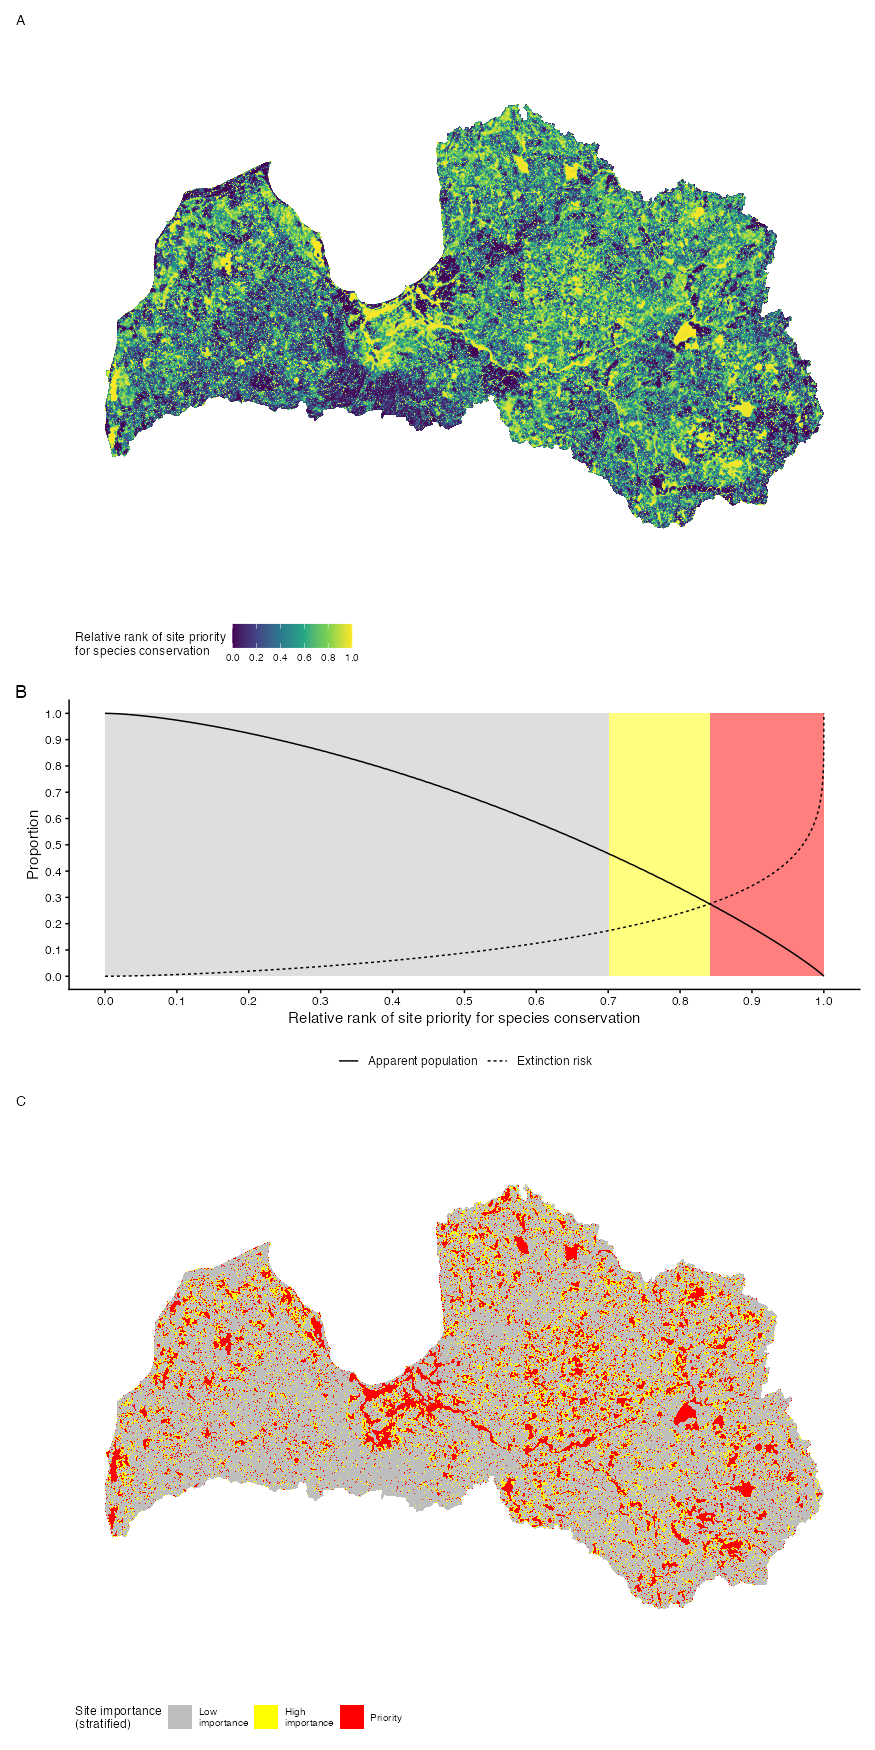
\includegraphics[width=0.85\linewidth,height=0.70\textheight,keepaspectratio]{results/RANARVmonitoringv2b5celi/PicPrior_RANARVmonitoring.png}

\par\small\textit{Single-species conservation prioritization focusing on maximisation of core area protection (CAZMAX) while accounting for site connectivity: (A) relative site rank; (B) relationship between apparent-population and extinction-risk curves with a simplified classification which is spatially demonstrated in the bootom row; (C) spatial distribution of proposed classification of site prioritization results. **For a full resolution refer to repository: link or online document: link**}\normalsize
\end{center}

\chapter*{\texorpdfstring{\emph{Pelophylax sp.}}{Pelophylax sp.}}\label{pelspp}
\addcontentsline{toc}{chapter}{\emph{Pelophylax sp.}}

\section*{Summary}\label{summary-21}
\addcontentsline{toc}{section}{Summary}

\subsection*{Model description}\label{model-description-21}
\addcontentsline{toc}{subsection}{Model description}

Occurrence and background data were divided into model-training with four block spatial cross-validation data and an independent test set. Sampling-bias/background treatment: \textbf{Phenology Weighted Target Group}. Accumulated LULC change within the 1-ha analysis cell was not evaluated; accumulated LULC change within the home-range radius around the analysis cell was not evaluated.

The final data set contained \textbf{2110} presence records: \textbf{1582} for training with four spatial block cross-validation and \textbf{528} for independent testing. Training background contained \textbf{29996} locations, with \textbf{10004} additional independent-test background locations.

\subsection*{Expert assessment scores}\label{expert-assessment-scores-21}
\addcontentsline{toc}{subsection}{Expert assessment scores}

\begin{itemize}
\tightlist
\item
  \textbf{Marginal responses and variable importance score:} 4 (good ecological interpretability)
\item
  \textbf{Map score:} 3 (moderate agreement with known distribution)
\item
  \textbf{Applicability score:} 3 (moderate applicability)
\end{itemize}

\textbf{Šo sadaļu aizpildām manuāli no ekspertu aptaujām}

\subsection*{Statistical evaluation}\label{statistical-evaluation-21}
\addcontentsline{toc}{subsection}{Statistical evaluation}

The final model had a training TSS of \textbf{0.401}, with a training-derived cloglog threshold of \textbf{0.532}. Combined training AUC was \textbf{0.818} and combined test AUC was \textbf{0.803}.

\subsubsection*{Spatial cross-validation}\label{spatial-cross-validation-21}
\addcontentsline{toc}{subsubsection}{Spatial cross-validation}

\begin{itemize}
\tightlist
\item
  \textbf{AUC:} 0.8247 ± 0.0127; null models: 0.5416 ± 0.0184; z = 15.3812, p \textless{} 0.001
\item
  \textbf{CBI:} 0.9885 ± 0.0062; null models: 0.4961 ± 0.1535; z = 3.2087, p = 0.001
\item
  \textbf{OR10:} 0.0917 ± 0.031; null models: 0.0382 ± 0.0306; z = 1.7483, p = 0.96
\item
  \textbf{ORmin:} 0.0025 ± 0.0051; null models: 0.001 ± 0.0053; z = 0.2896, p = 0.614
\end{itemize}

\subsubsection*{Independent testing}\label{independent-testing-21}
\addcontentsline{toc}{subsubsection}{Independent testing}

\begin{itemize}
\tightlist
\item
  \textbf{TSS:} 0.47; \textbf{sensitivity:} 0.79; \textbf{specificity:} 0.68
\item
  \textbf{AUC:} 0.816; null models: 0.5773 ± 0.0628; z = 3.8011, p \textless{} 0.001
\item
  \textbf{CBI:} 0.991; null models: 0.4301 ± 0.4042; z = 1.3875, p = 0.083
\item
  \textbf{OR10:} 0.091; null models: 0.0532 ± 0.0352; z = 1.0713, p = 0.858
\item
  \textbf{ORmin:} 0.002; null models: 5e-04 ± 0.0012; z = 1.1247, p = 0.87
\end{itemize}

\subsection*{Conservation prioritisation summary}\label{conservation-prioritisation-summary-21}
\addcontentsline{toc}{subsection}{Conservation prioritisation summary}

The primary priority area covers \textbf{13.8\%} of Latvia and contains \textbf{27.6\%} of the summed habitat suitability (apparent population proxy).

The broader high importance area covers \textbf{26.3\%} of Latvia and contains \textbf{46\%} of the summed habitat suitability.

For comparison, the area classified as suitable using the maximum training sensitivity plus specificity habitat-suitability threshold contains \textbf{46\%} of the summed continuous habitat suitability.

\subsection*{Version evolution}\label{version-evolution-21}
\addcontentsline{toc}{subsection}{Version evolution}

\textbf{Šo sadaļu aizpildām manuāli, izmntojot sagatavotās shēmas. Jāvienojas par to noformējumu}

\section*{Habitat suitability}\label{habitat-suitability-21}
\addcontentsline{toc}{section}{Habitat suitability}

\begin{center}
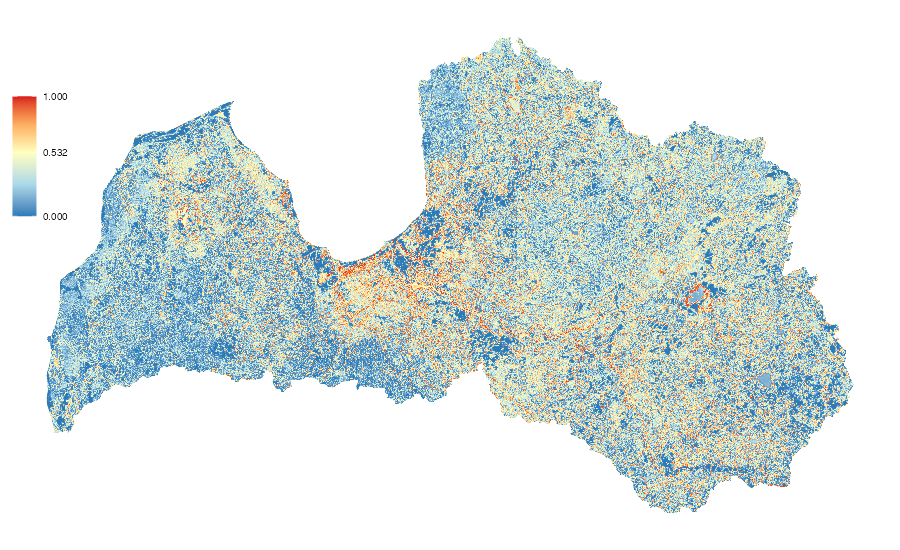
\includegraphics[width=1\linewidth,height=0.70\textheight,keepaspectratio]{results/PELSPPv3b/PicHSmap_PELSPP.png}

\par\small\textit{Predicted continuous habitat suitability across Latvia. The warmer the colour the higher is the predicted habitat suitability. Value in the middle of the legend correspond to the maximum training sensitivity plus specificity threshold. **For a full resolution refer to repository: link or online document: link**}\normalsize
\end{center}

\section*{Model thresholds}\label{model-thresholds-21}
\addcontentsline{toc}{section}{Model thresholds}

Threshold values and associated omission rates

\begin{center}
\resizebox{\linewidth}{!}{%

\begin{tabular}{lrrrrr}
\toprule
Threshold & Cloglog value & Fractional predicted area & Training omission rate & Test omission rate & P-values\\
\midrule
Minimum training presence & 0.0004057 & 0.9981705 & 0.0000000 & 0.0000915 & 0\\
Equal training sensitivity and specificity & 0.5850717 & 0.2503210 & 0.2503161 & 0.0118056 & 0\\
Maximum training sensitivity plus specificity & 0.5316696 & 0.2998459 & 0.1940582 & 0.0101583 & 0\\
Equal test sensitivity and specificity & 0.5983189 & 0.2380922 & 0.2623262 & 0.0122632 & 0\\
Maximum test sensitivity plus specificity & 0.5970316 & 0.2397612 & 0.2604298 & 0.0121717 & 0\\
\bottomrule
\end{tabular}
}
\end{center}

\section*{Variable importance}\label{variable-importance-21}
\addcontentsline{toc}{section}{Variable importance}

\begin{center}
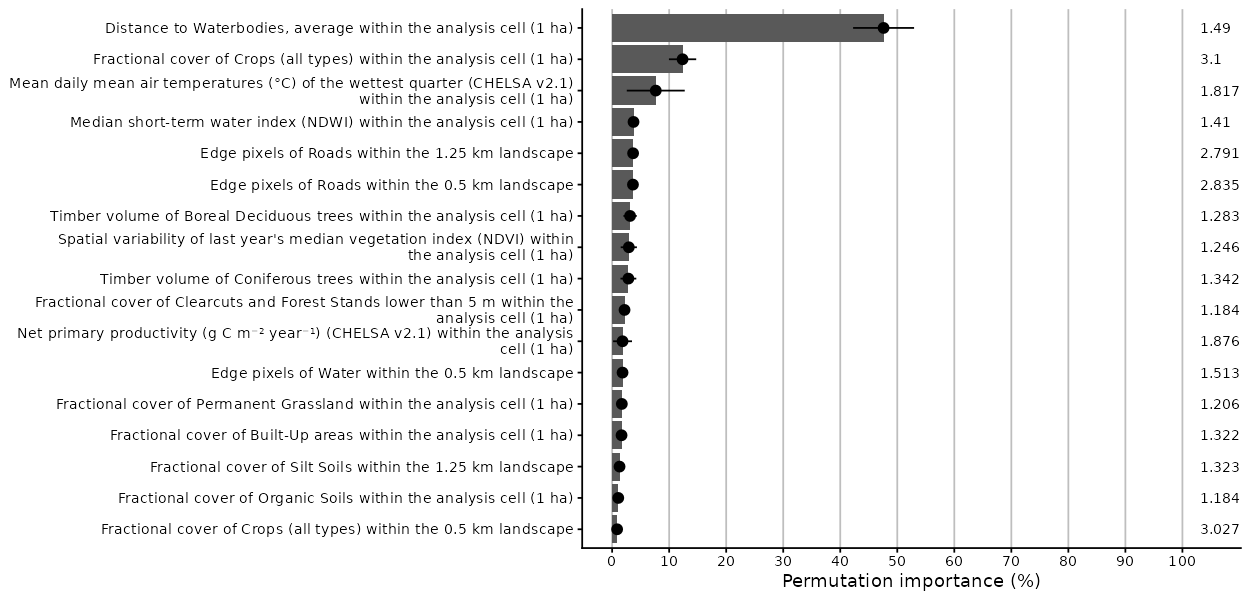
\includegraphics[width=1\linewidth,height=0.70\textheight,keepaspectratio]{results/PELSPPv3b/PicVarImpVIFs_PELSPP.png}

\par\small\textit{Permutation-importance (mean and standard deviation from 99 permutations, on the x-axis) of the ecogeographical variables (first y-axis, left side), and their variance inflation factor values (second y-axis, right side). **For a full resolution refer to repository: link or online document: link**}\normalsize
\end{center}

\section*{Marginal responses}\label{marginal-responses-21}
\addcontentsline{toc}{section}{Marginal responses}

\begin{center}
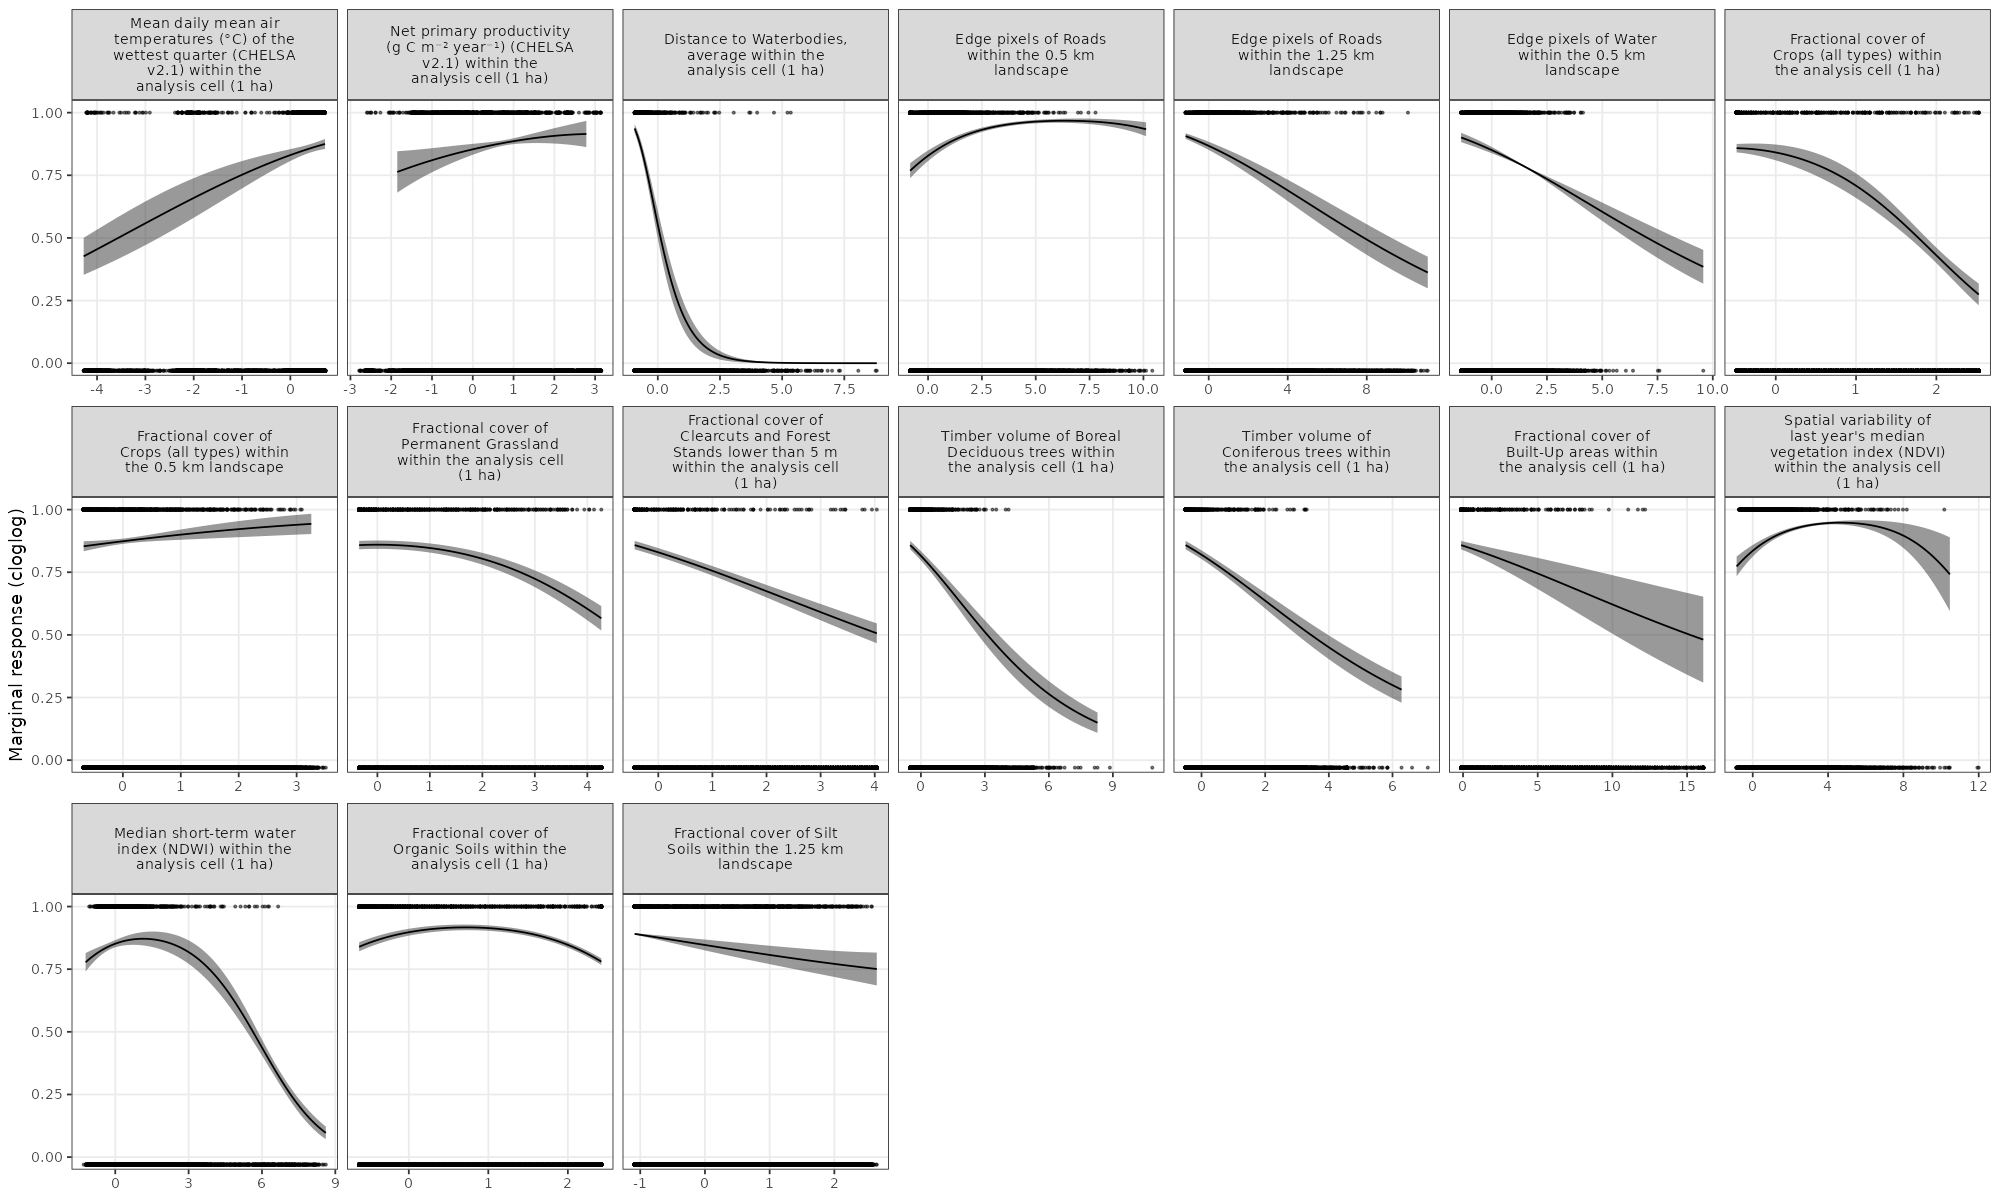
\includegraphics[width=1\linewidth,height=0.70\textheight,keepaspectratio]{results/PELSPPv3b/PicMargResp_PELSPP.png}

\par\small\textit{Marginalised for arithmetic mean response curves illustrating the effect of each ecogeographical variable on the habitat suitability when all the other variables have their arithmetic mean values. The y-axis shows the predicted habitat suitability (cloglog-transformed), while the x-axis shows the standardised (centred and scaled) value of the ecogeographical variable. Dots at a value of 1 on the y-axis illustrate presence locations in the environment (on the x-axis), while dots at a value of 0 illustrate background locations used in modelling.  **For a full resolution refer to repository: link or online document: link**}\normalsize
\end{center}

\section*{Habitat and conservation associations}\label{habitat-and-conservation-associations-21}
\addcontentsline{toc}{section}{Habitat and conservation associations}

\begin{center}
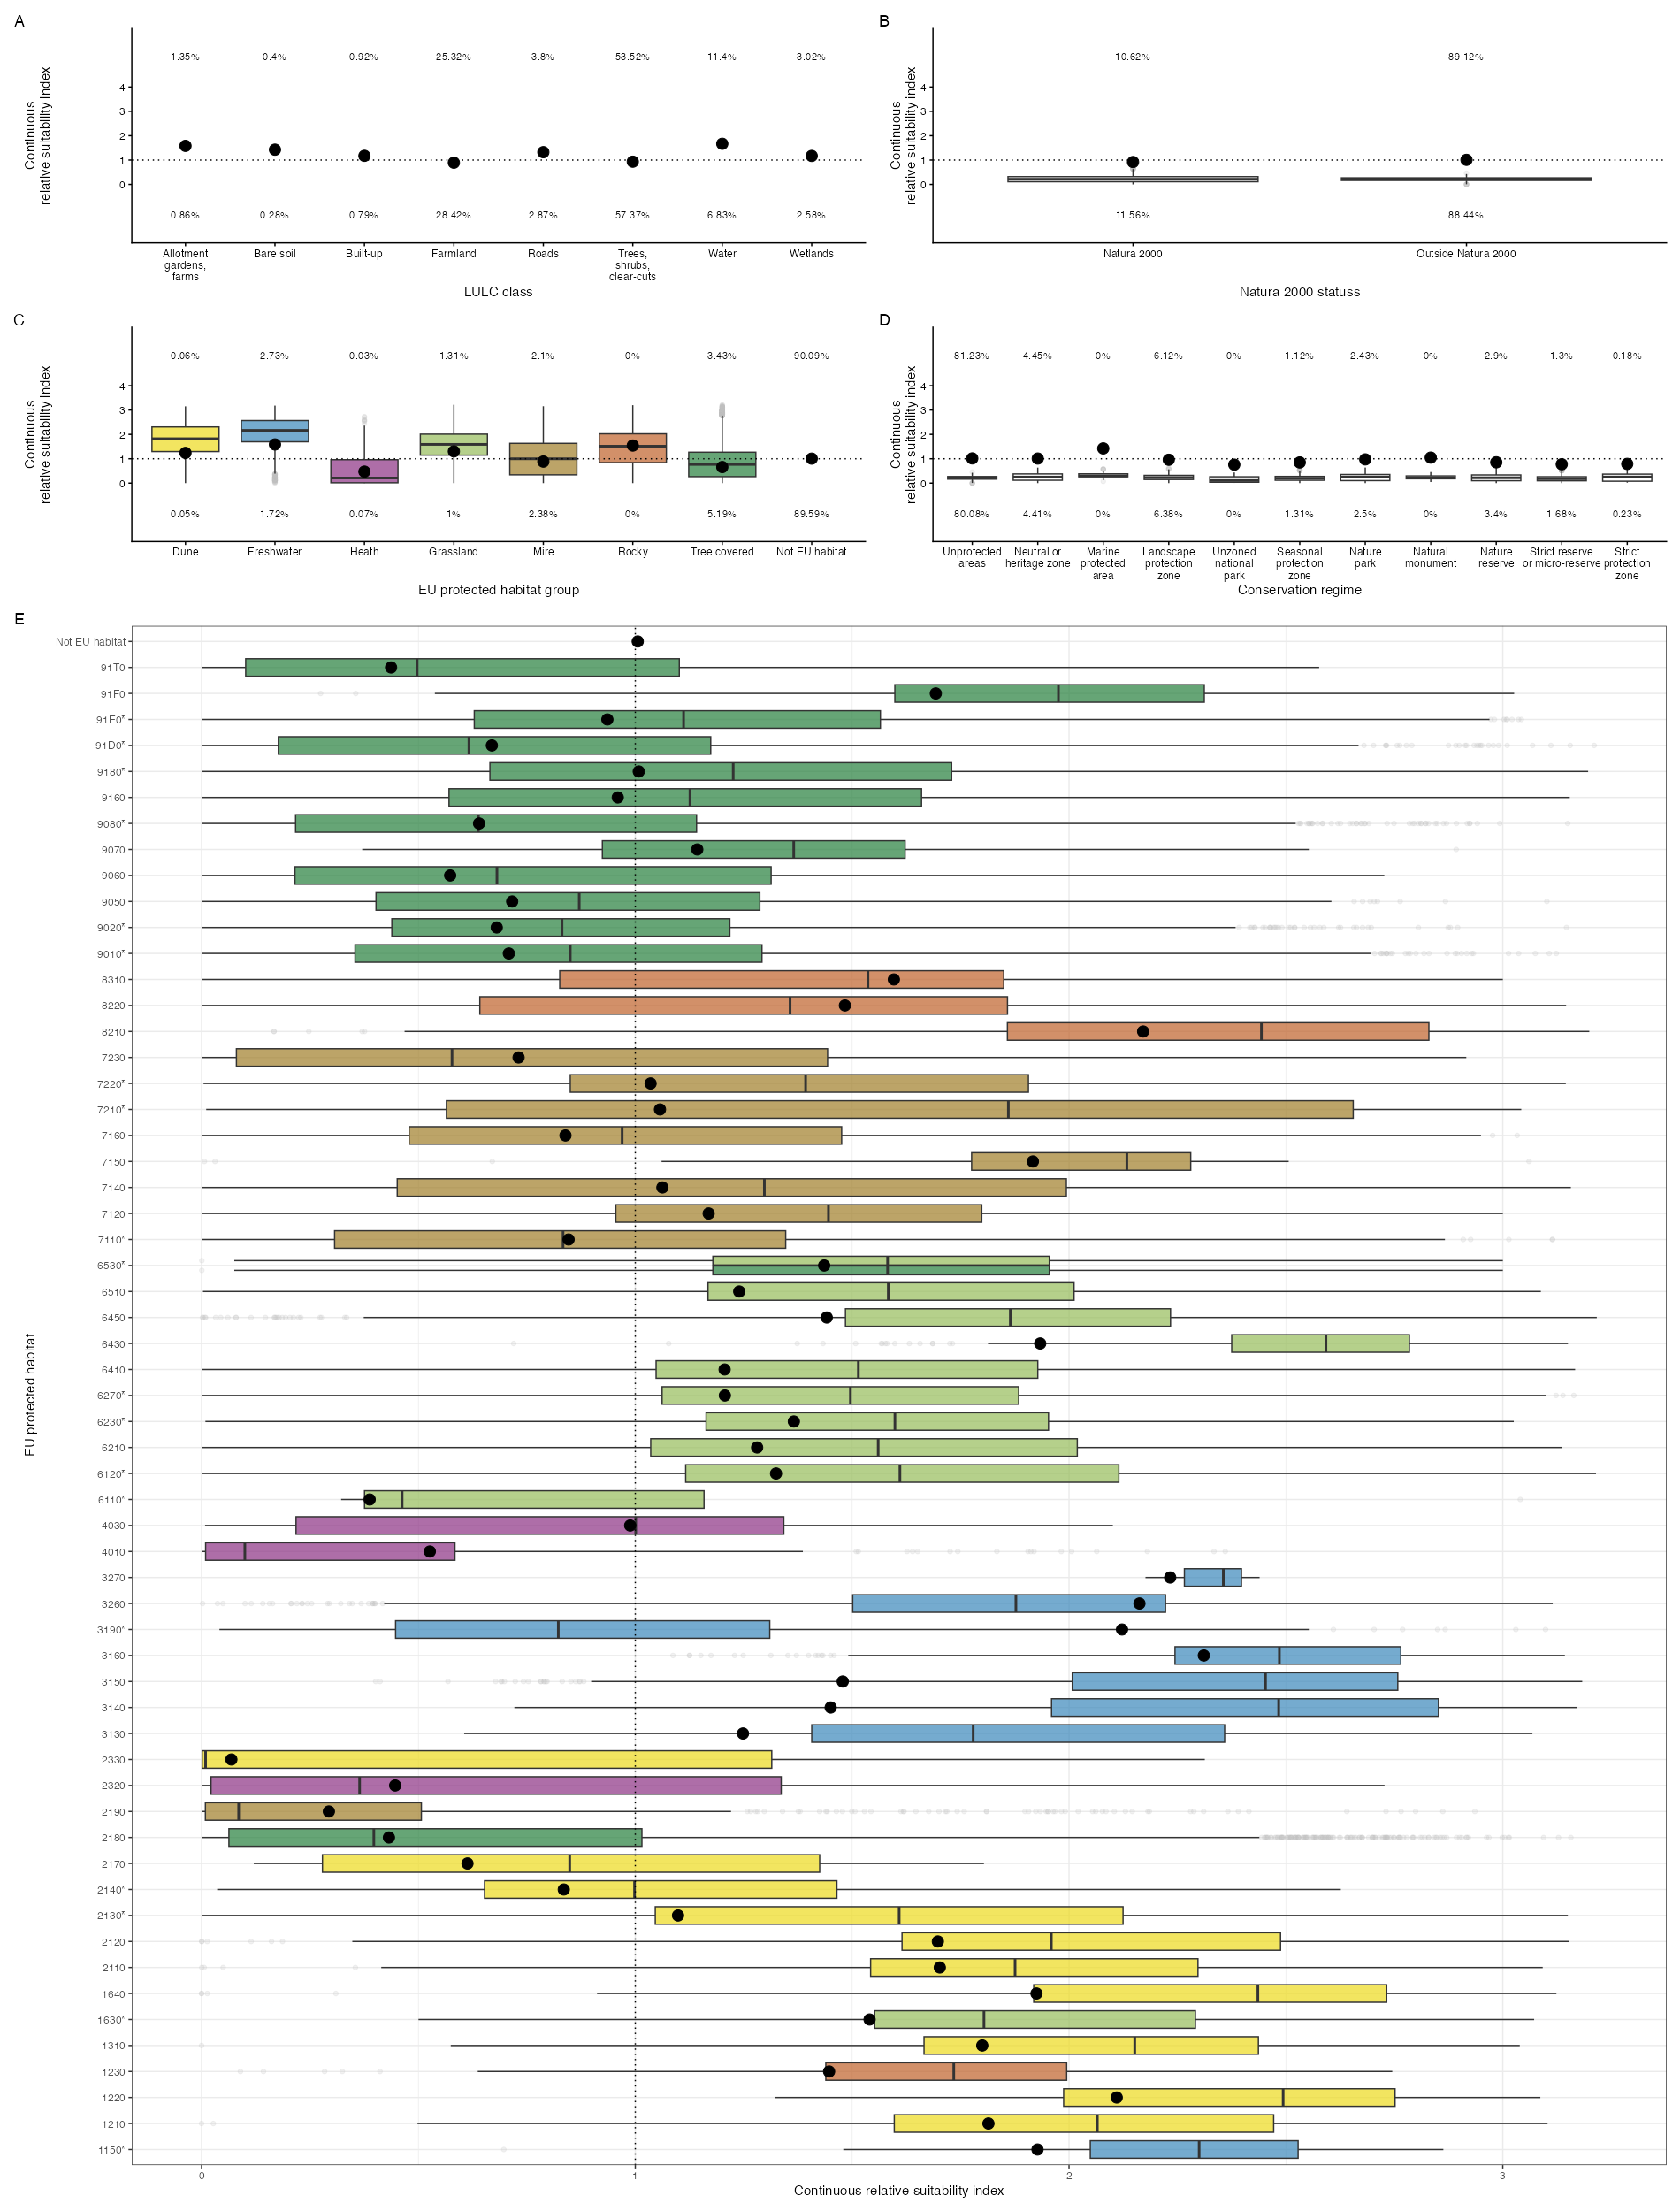
\includegraphics[width=1\linewidth,height=0.70\textheight,keepaspectratio]{results/PELSPPv3b/PicAssoc_PELSPP.png}

\par\small\textit{Associations between predicted suitability and: (A) land use land cover classes, (B) Natura 2000 status, (C) stratified EU protected habitat classes, (D) conservation regime, and (E) EU protected habitats. The y-axis show continuous relative suitability index (derivative of Manly's index of preference). Colours in (C) and (E) correspond to stratified EU protected habitat classes. For classifications composed of multiple individual polygons, polygon-level indices were additionally calculated to show within-category variation. The figures therefore combine category-level estimates (points) with the distributions of polygon-level values (boxplots, where applicable). Labels above and below the panels report, respectively, the percentage of total predicted suitability and the percentage of mapped area represented by each category. **For a full resolution refer to repository: link or online document: link**}\normalsize
\end{center}

\section*{Conservation prioritization}\label{conservation-prioritization-21}
\addcontentsline{toc}{section}{Conservation prioritization}

\begin{center}
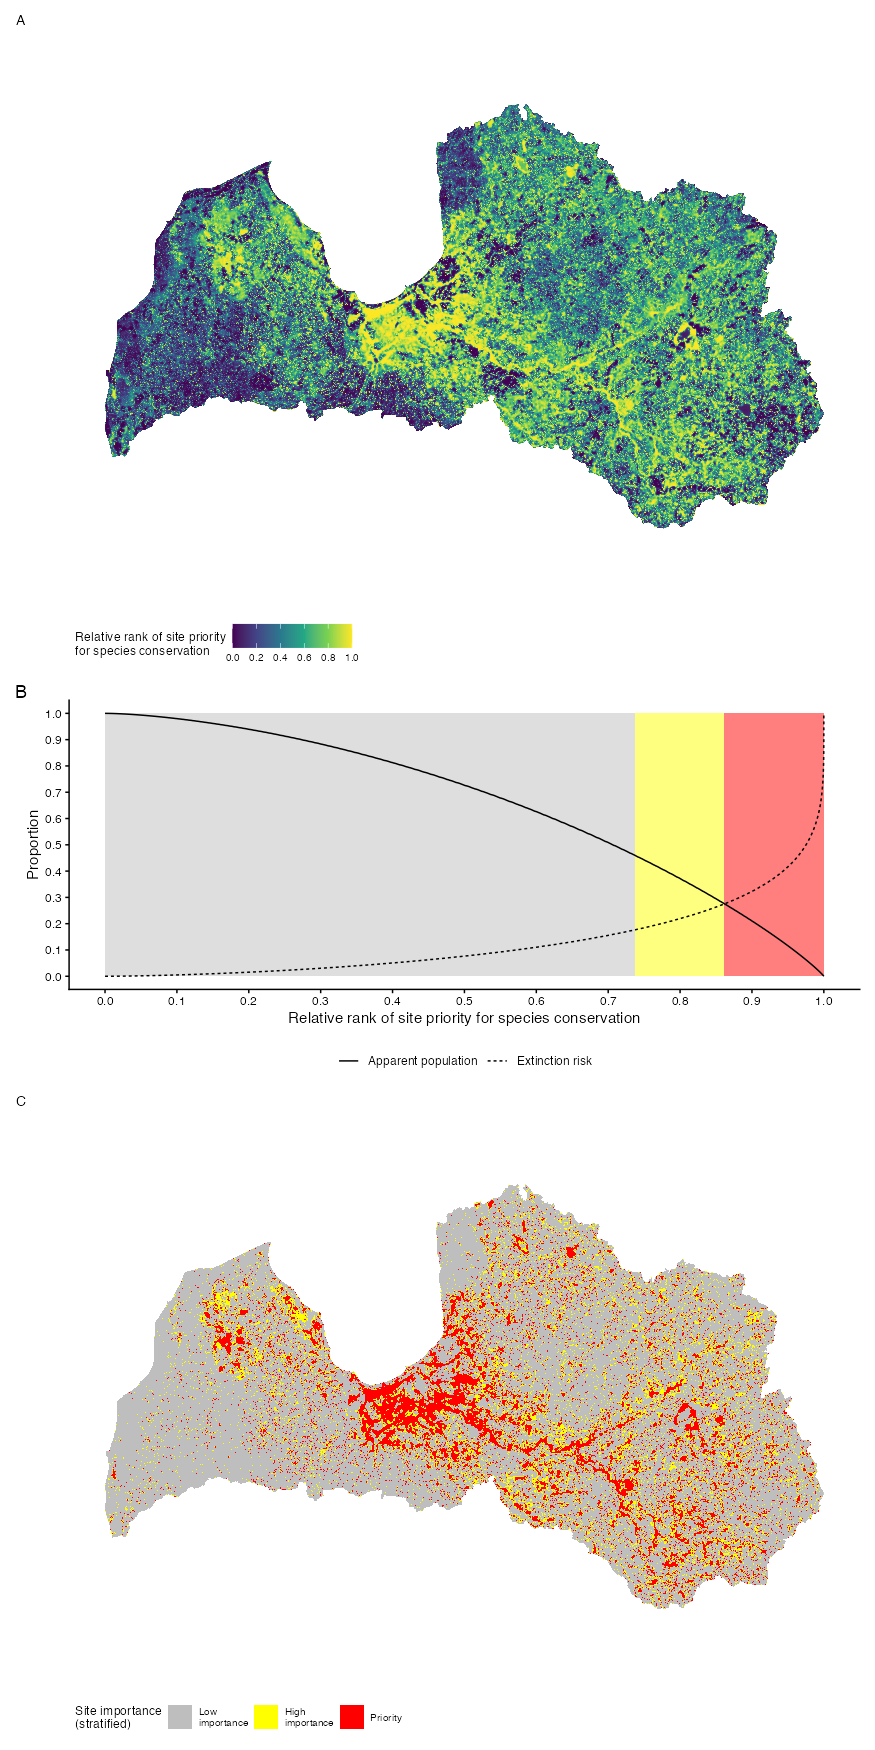
\includegraphics[width=0.85\linewidth,height=0.70\textheight,keepaspectratio]{results/PELSPPv3b/PicPrior_PELSPP.png}

\par\small\textit{Single-species conservation prioritization focusing on maximisation of core area protection (CAZMAX) while accounting for site connectivity: (A) relative site rank; (B) relationship between apparent-population and extinction-risk curves with a simplified classification which is spatially demonstrated in the bootom row; (C) spatial distribution of proposed classification of site prioritization results. **For a full resolution refer to repository: link or online document: link**}\normalsize
\end{center}

\chapter*{\texorpdfstring{\emph{Pelophylax sp.} monitoring}{Pelophylax sp. monitoring}}\label{pelsppmonitoring}
\addcontentsline{toc}{chapter}{\emph{Pelophylax sp.} monitoring}

\section*{Summary}\label{summary-22}
\addcontentsline{toc}{section}{Summary}

\subsection*{Model description}\label{model-description-22}
\addcontentsline{toc}{subsection}{Model description}

Occurrence and background data were divided into model-training with four block spatial cross-validation data and an independent test set. Sampling-bias/background treatment: \textbf{Phenology Weighted Target Group}. Accumulated LULC change within the 1-ha analysis cell was not evaluated; accumulated LULC change within the home-range radius around the analysis cell was not evaluated.

The final data set contained \textbf{1701} presence records: \textbf{1276} for training with four spatial block cross-validation and \textbf{425} for independent testing. Training background contained \textbf{30007} locations, with \textbf{9993} additional independent-test background locations.

\subsection*{Expert assessment scores}\label{expert-assessment-scores-22}
\addcontentsline{toc}{subsection}{Expert assessment scores}

\begin{itemize}
\tightlist
\item
  \textbf{Marginal responses and variable importance score:} 4 (good ecological interpretability)
\item
  \textbf{Map score:} 3 (moderate agreement with known distribution)
\item
  \textbf{Applicability score:} 3 (moderate applicability)
\end{itemize}

\textbf{Šo sadaļu aizpildām manuāli no ekspertu aptaujām}

\subsection*{Statistical evaluation}\label{statistical-evaluation-22}
\addcontentsline{toc}{subsection}{Statistical evaluation}

The final model had a training TSS of \textbf{0.401}, with a training-derived cloglog threshold of \textbf{0.489}. Combined training AUC was \textbf{0.836} and combined test AUC was \textbf{0.814}.

\subsubsection*{Spatial cross-validation}\label{spatial-cross-validation-22}
\addcontentsline{toc}{subsubsection}{Spatial cross-validation}

\begin{itemize}
\tightlist
\item
  \textbf{AUC:} 0.8407 ± 0.0291; null models: 0.5811 ± 0.0209; z = 12.4341, p \textless{} 0.001
\item
  \textbf{CBI:} 0.988 ± 0.0174; null models: 0.5555 ± 0.1755; z = 2.4648, p = 0.007
\item
  \textbf{OR10:} 0.0957 ± 0.0296; null models: 0.0217 ± 0.0311; z = 2.3822, p = 0.991
\item
  \textbf{ORmin:} 0.0039 ± 0.0078; null models: 1e-04 ± 7e-04; z = 5.5135, p = 1
\end{itemize}

\subsubsection*{Independent testing}\label{independent-testing-22}
\addcontentsline{toc}{subsubsection}{Independent testing}

\begin{itemize}
\tightlist
\item
  \textbf{TSS:} 0.49; \textbf{sensitivity:} 0.835; \textbf{specificity:} 0.655
\item
  \textbf{AUC:} 0.858; null models: 0.6149 ± 0.1117; z = 2.1758, p = 0.015
\item
  \textbf{CBI:} 0.993; null models: 0.4685 ± 0.5504; z = 0.953, p = 0.17
\item
  \textbf{OR10:} 0.094; null models: 0.0451 ± 0.048; z = 1.0219, p = 0.847
\item
  \textbf{ORmin:} 0; null models: 2e-04 ± 0.0014; z = -0.1378, p = 0.445
\end{itemize}

\subsection*{Conservation prioritisation summary}\label{conservation-prioritisation-summary-22}
\addcontentsline{toc}{subsection}{Conservation prioritisation summary}

The primary priority area covers \textbf{11.5\%} of Latvia and contains \textbf{27.6\%} of the summed habitat suitability (apparent population proxy).

The broader high importance area covers \textbf{25.4\%} of Latvia and contains \textbf{49.9\%} of the summed habitat suitability.

For comparison, the area classified as suitable using the maximum training sensitivity plus specificity habitat-suitability threshold contains \textbf{49.9\%} of the summed continuous habitat suitability.

\subsection*{Version evolution}\label{version-evolution-22}
\addcontentsline{toc}{subsection}{Version evolution}

\textbf{Šo sadaļu aizpildām manuāli, izmntojot sagatavotās shēmas. Jāvienojas par to noformējumu}

\section*{Habitat suitability}\label{habitat-suitability-22}
\addcontentsline{toc}{section}{Habitat suitability}

\begin{center}
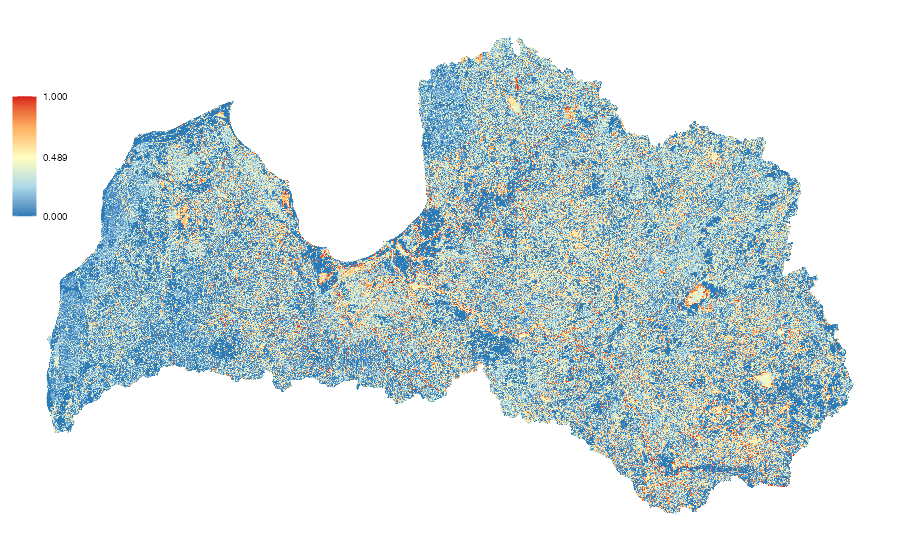
\includegraphics[width=1\linewidth,height=0.70\textheight,keepaspectratio]{results/PELSPPmonitoring_v2b1/PicHSmap_PELSPPmonitoring.png}

\par\small\textit{Predicted continuous habitat suitability across Latvia. The warmer the colour the higher is the predicted habitat suitability. Value in the middle of the legend correspond to the maximum training sensitivity plus specificity threshold. **For a full resolution refer to repository: link or online document: link**}\normalsize
\end{center}

\section*{Model thresholds}\label{model-thresholds-22}
\addcontentsline{toc}{section}{Model thresholds}

Threshold values and associated omission rates

\begin{center}
\resizebox{\linewidth}{!}{%

\begin{tabular}{lrrrrr}
\toprule
Threshold & Cloglog value & Fractional predicted area & Training omission rate & Test omission rate & P-values\\
\midrule
Minimum training presence & 0.0000110 & 0.9947426 & 0.0000000 & 0.0000000 & 0\\
Equal training sensitivity and specificity & 0.5370237 & 0.2373272 & 0.2374608 & 0.0075892 & 0\\
Maximum training sensitivity plus specificity & 0.4886590 & 0.2758162 & 0.1849530 & 0.0065586 & 0\\
Equal test sensitivity and specificity & 0.6098725 & 0.1827741 & 0.3079937 & 0.0100253 & 0\\
Maximum test sensitivity plus specificity & 0.5845637 & 0.2012721 & 0.2782132 & 0.0086199 & 0\\
\bottomrule
\end{tabular}
}
\end{center}

\section*{Variable importance}\label{variable-importance-22}
\addcontentsline{toc}{section}{Variable importance}

\begin{center}
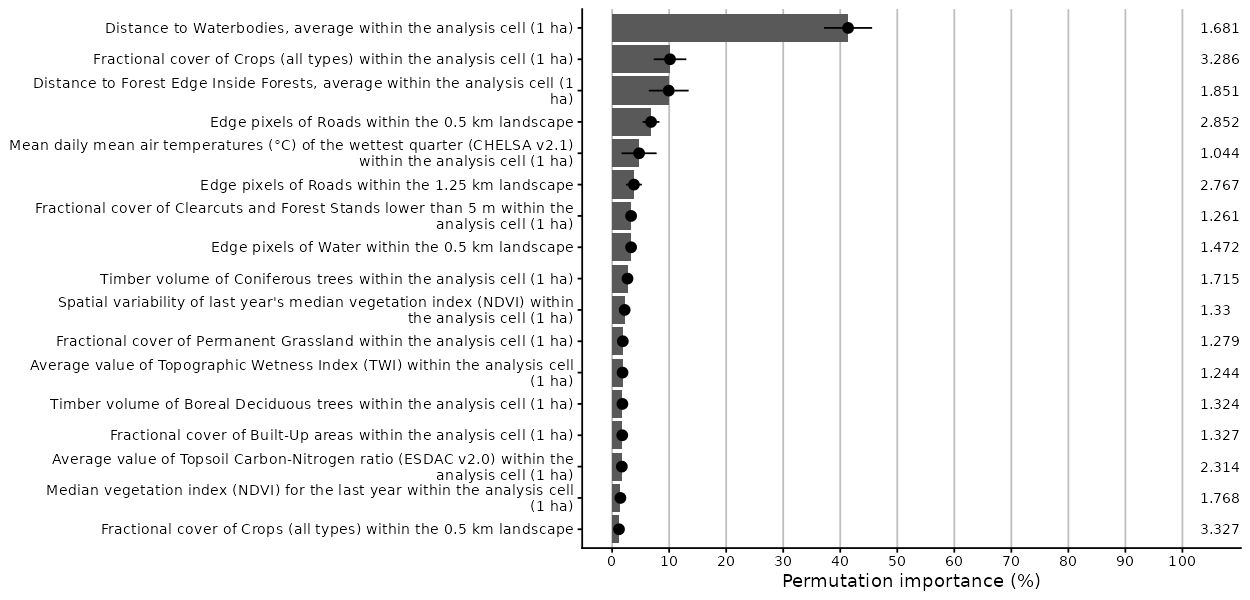
\includegraphics[width=1\linewidth,height=0.70\textheight,keepaspectratio]{results/PELSPPmonitoring_v2b1/PicVarImpVIFs_PELSPPmonitoring.png}

\par\small\textit{Permutation-importance (mean and standard deviation from 99 permutations, on the x-axis) of the ecogeographical variables (first y-axis, left side), and their variance inflation factor values (second y-axis, right side). **For a full resolution refer to repository: link or online document: link**}\normalsize
\end{center}

\section*{Marginal responses}\label{marginal-responses-22}
\addcontentsline{toc}{section}{Marginal responses}

\begin{center}
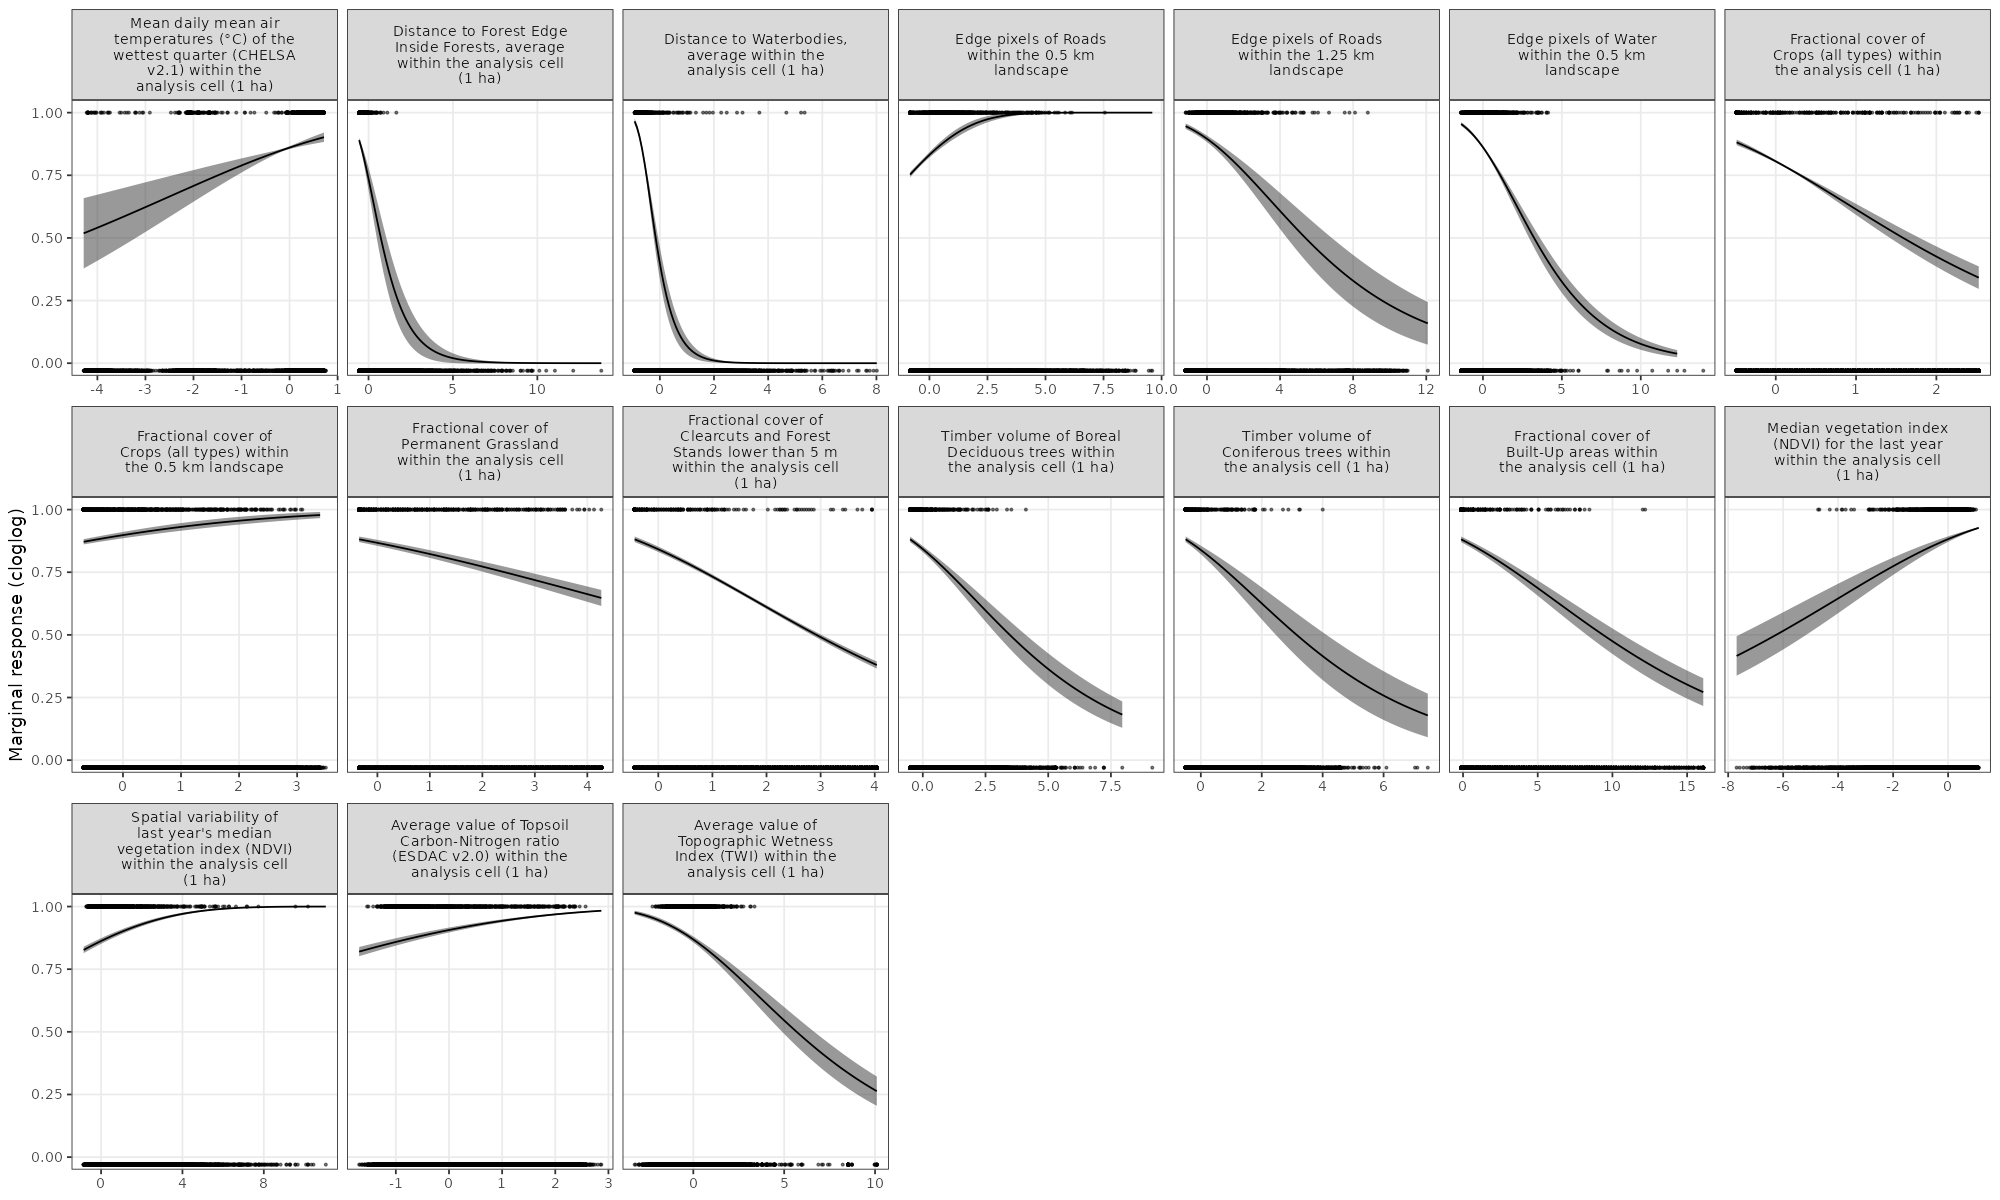
\includegraphics[width=1\linewidth,height=0.70\textheight,keepaspectratio]{results/PELSPPmonitoring_v2b1/PicMargResp_PELSPPmonitoring.png}

\par\small\textit{Marginalised for arithmetic mean response curves illustrating the effect of each ecogeographical variable on the habitat suitability when all the other variables have their arithmetic mean values. The y-axis shows the predicted habitat suitability (cloglog-transformed), while the x-axis shows the standardised (centred and scaled) value of the ecogeographical variable. Dots at a value of 1 on the y-axis illustrate presence locations in the environment (on the x-axis), while dots at a value of 0 illustrate background locations used in modelling.  **For a full resolution refer to repository: link or online document: link**}\normalsize
\end{center}

\section*{Habitat and conservation associations}\label{habitat-and-conservation-associations-22}
\addcontentsline{toc}{section}{Habitat and conservation associations}

\begin{center}
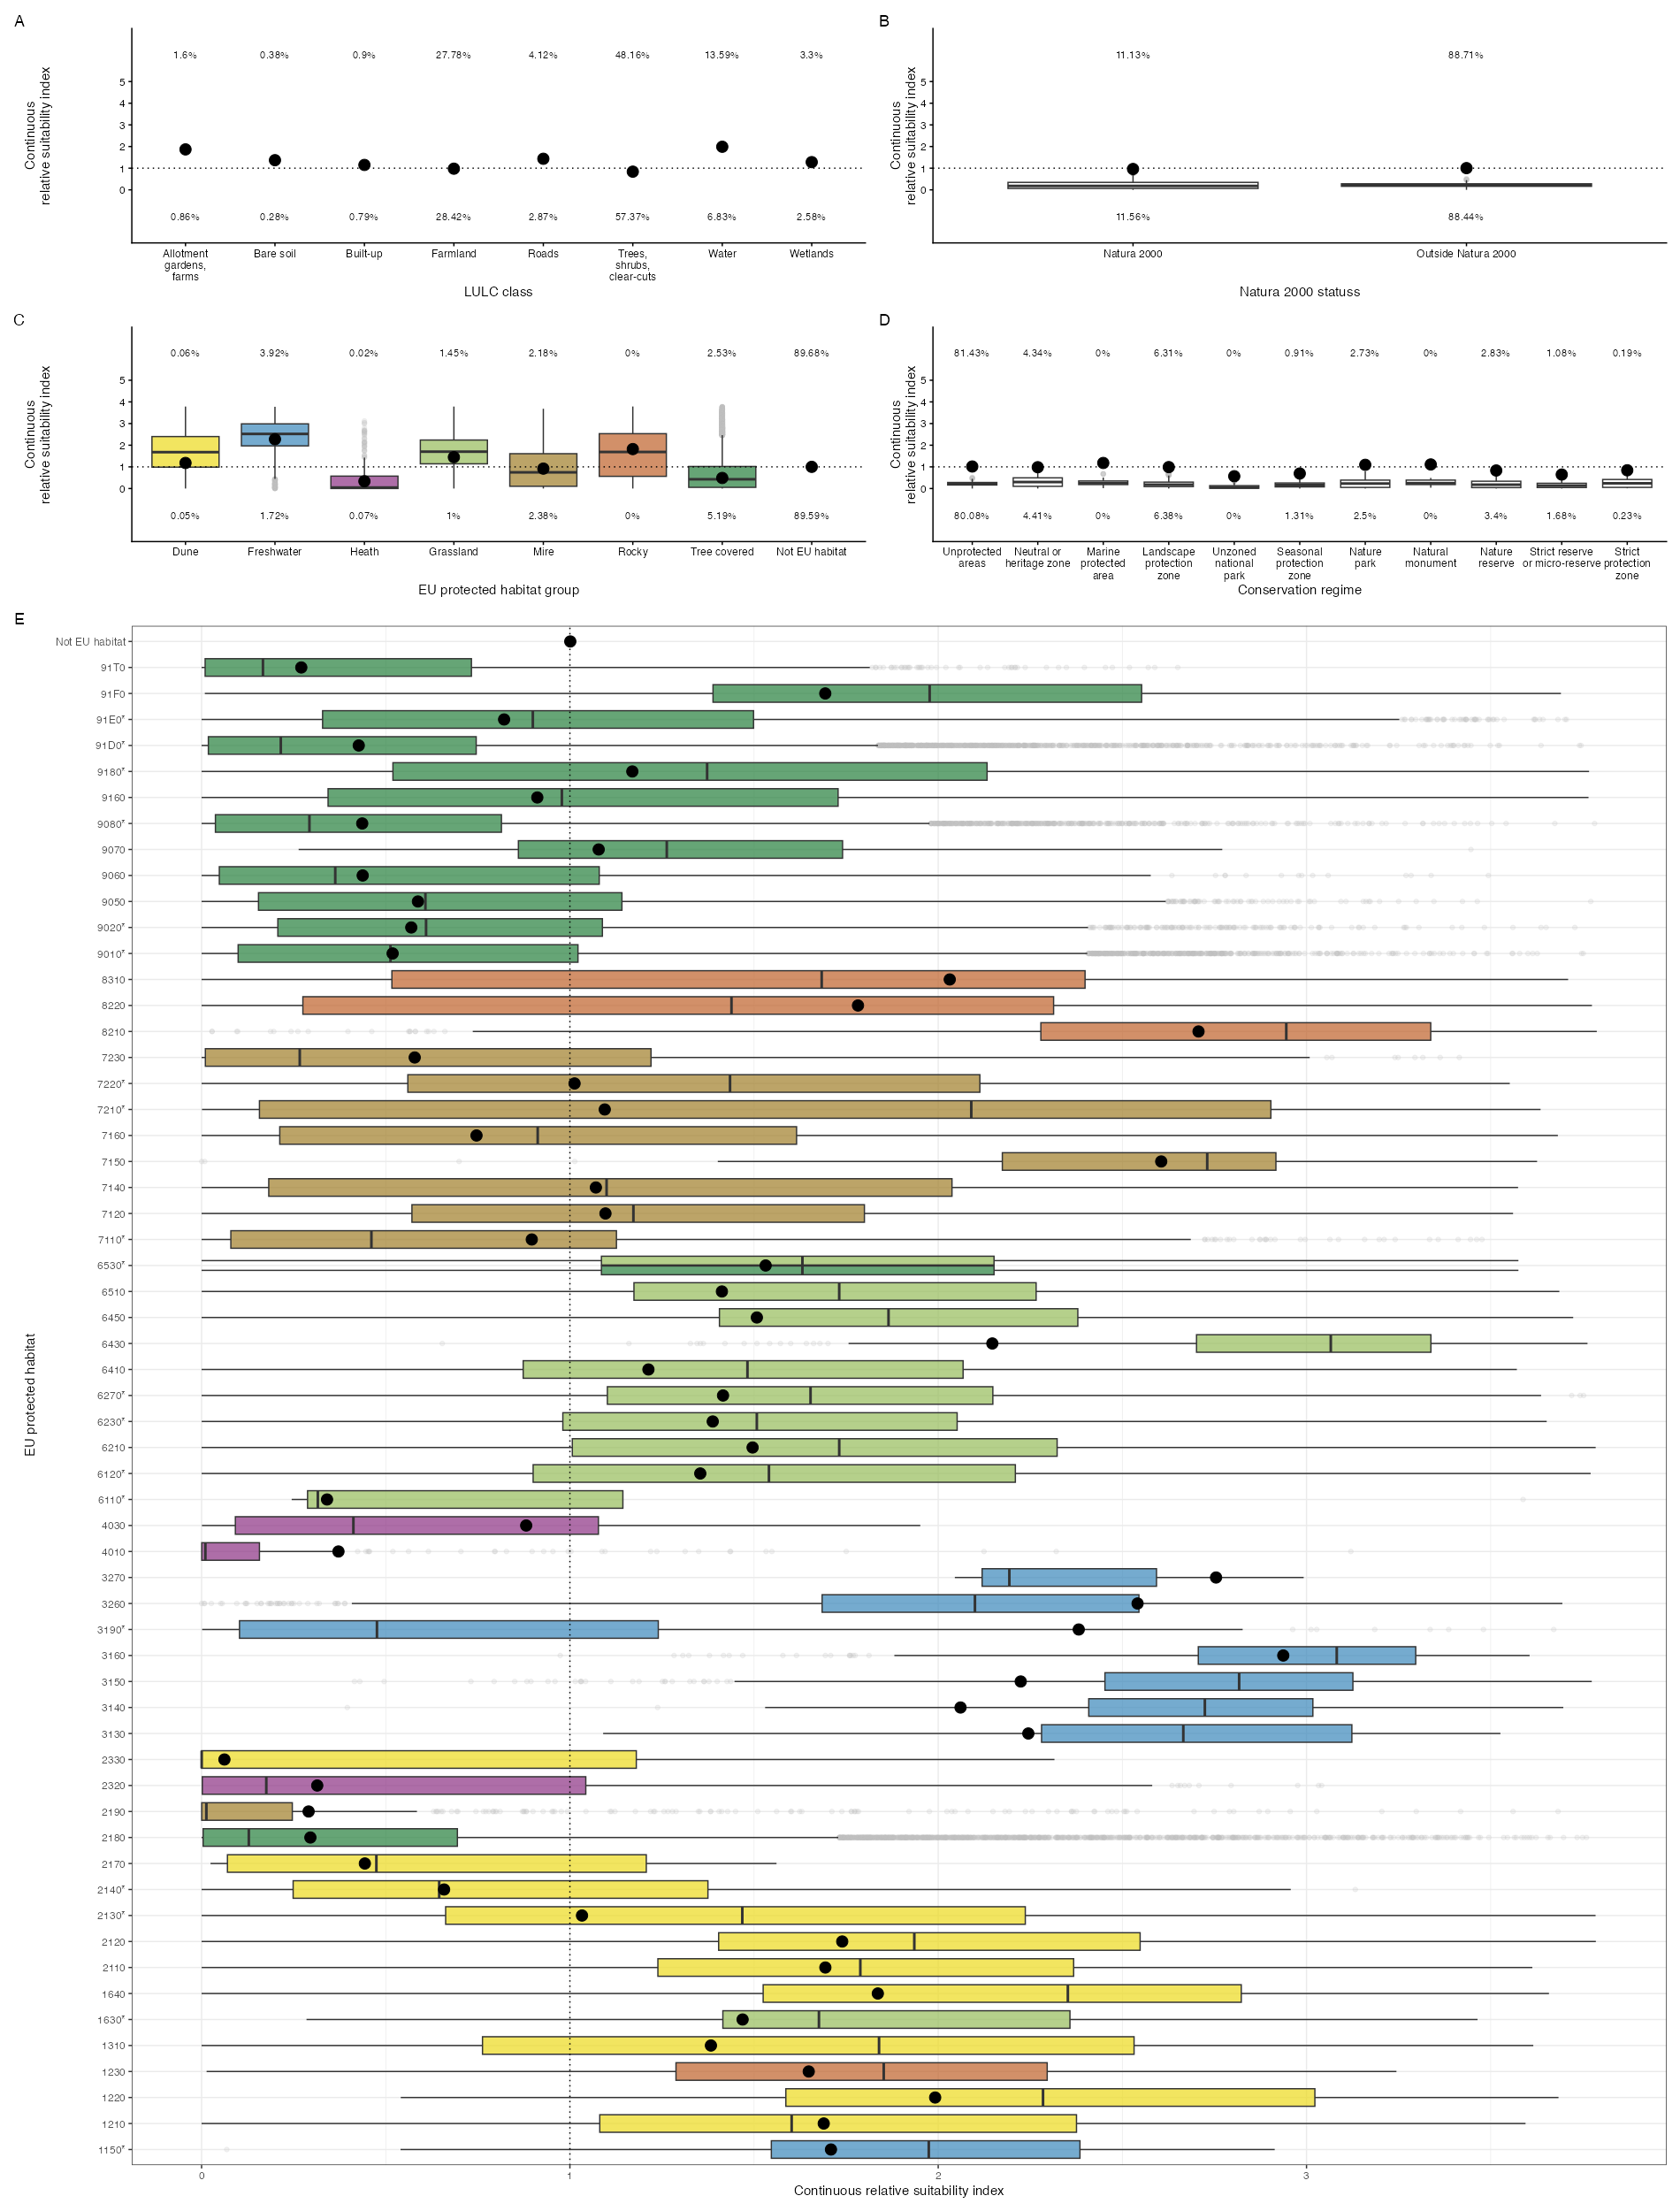
\includegraphics[width=1\linewidth,height=0.70\textheight,keepaspectratio]{results/PELSPPmonitoring_v2b1/PicAssoc_PELSPPmonitoring.png}

\par\small\textit{Associations between predicted suitability and: (A) land use land cover classes, (B) Natura 2000 status, (C) stratified EU protected habitat classes, (D) conservation regime, and (E) EU protected habitats. The y-axis show continuous relative suitability index (derivative of Manly's index of preference). Colours in (C) and (E) correspond to stratified EU protected habitat classes. For classifications composed of multiple individual polygons, polygon-level indices were additionally calculated to show within-category variation. The figures therefore combine category-level estimates (points) with the distributions of polygon-level values (boxplots, where applicable). Labels above and below the panels report, respectively, the percentage of total predicted suitability and the percentage of mapped area represented by each category. **For a full resolution refer to repository: link or online document: link**}\normalsize
\end{center}

\section*{Conservation prioritization}\label{conservation-prioritization-22}
\addcontentsline{toc}{section}{Conservation prioritization}

\begin{center}
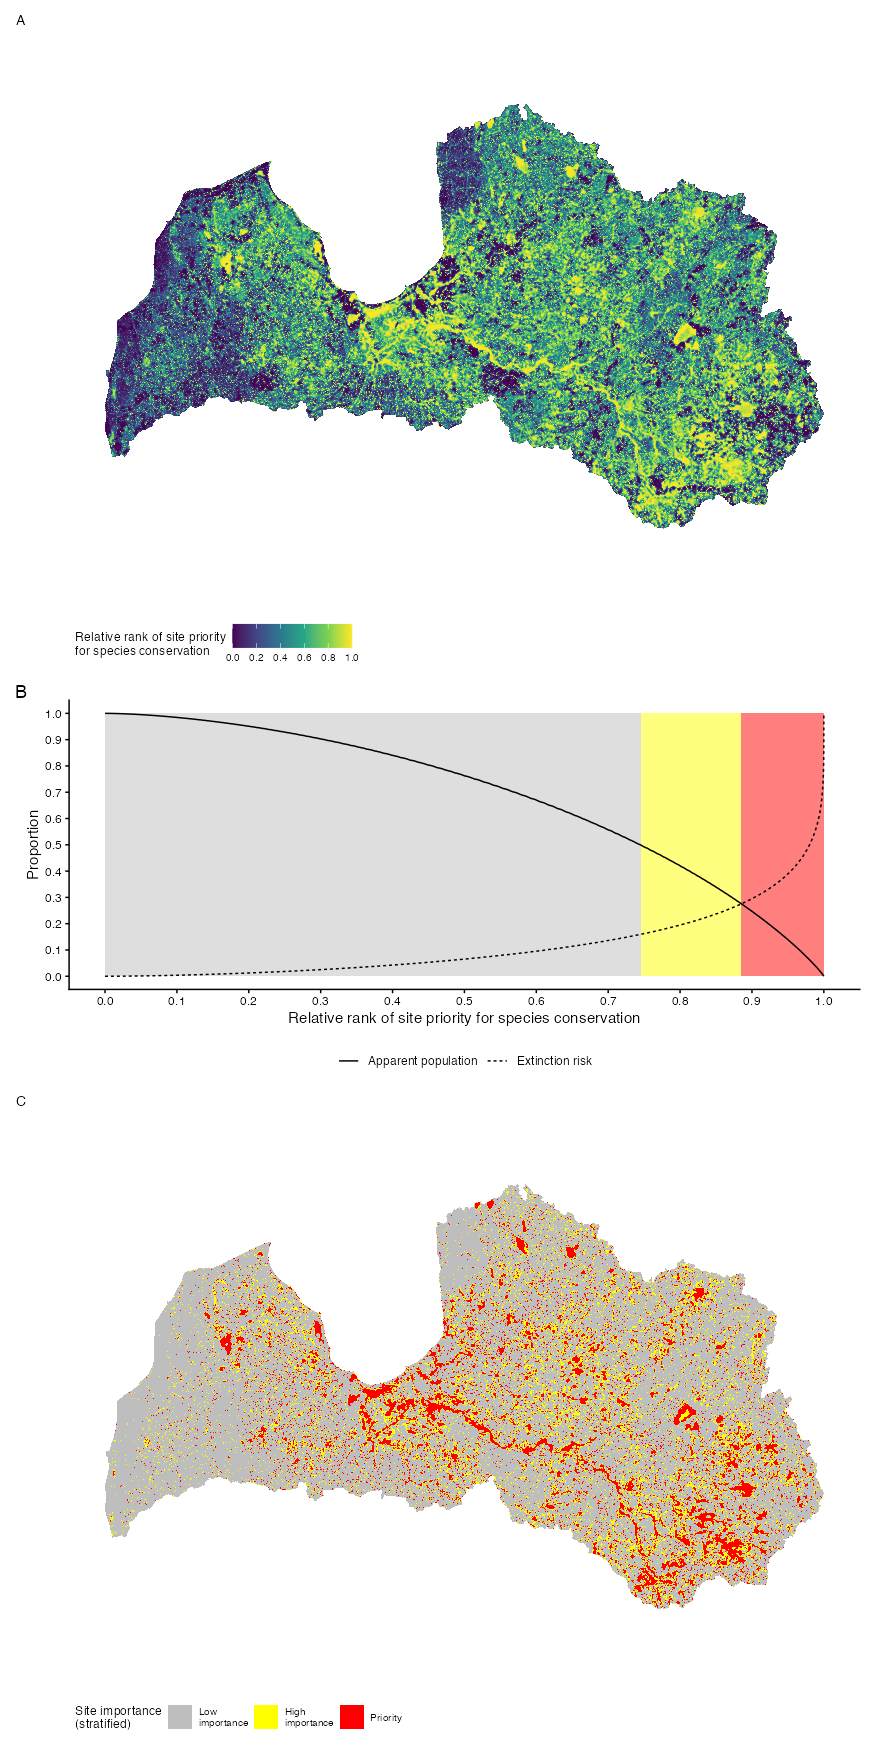
\includegraphics[width=0.85\linewidth,height=0.70\textheight,keepaspectratio]{results/PELSPPmonitoring_v2b1/PicPrior_PELSPPmonitoring.png}

\par\small\textit{Single-species conservation prioritization focusing on maximisation of core area protection (CAZMAX) while accounting for site connectivity: (A) relative site rank; (B) relationship between apparent-population and extinction-risk curves with a simplified classification which is spatially demonstrated in the bootom row; (C) spatial distribution of proposed classification of site prioritization results. **For a full resolution refer to repository: link or online document: link**}\normalsize
\end{center}

\chapter*{\texorpdfstring{\emph{Lacerta agilis}}{Lacerta agilis}}\label{lacagi}
\addcontentsline{toc}{chapter}{\emph{Lacerta agilis}}

\section*{Summary}\label{summary-23}
\addcontentsline{toc}{section}{Summary}

\subsection*{Model description}\label{model-description-23}
\addcontentsline{toc}{subsection}{Model description}

Occurrence and background data were divided into model-training with four block spatial cross-validation data and an independent test set. Sampling-bias/background treatment: \textbf{Phenology Weighted Target Group}. Accumulated LULC change within the 1-ha analysis cell was not evaluated; accumulated LULC change within the home-range radius around the analysis cell was not evaluated.

The final data set contained \textbf{457} presence records: \textbf{343} for training with four spatial block cross-validation and \textbf{114} for independent testing. Training background contained \textbf{29966} locations, with \textbf{10034} additional independent-test background locations.

\subsection*{Expert assessment scores}\label{expert-assessment-scores-23}
\addcontentsline{toc}{subsection}{Expert assessment scores}

\begin{itemize}
\tightlist
\item
  \textbf{Marginal responses and variable importance score:} 4 (good ecological interpretability)
\item
  \textbf{Map score:} 4 (good agreement with known distribution)
\item
  \textbf{Applicability score:} 4 (high applicability)
\end{itemize}

\textbf{Šo sadaļu aizpildām manuāli no ekspertu aptaujām}

\subsection*{Statistical evaluation}\label{statistical-evaluation-23}
\addcontentsline{toc}{subsection}{Statistical evaluation}

The final model had a training TSS of \textbf{0.401}, with a training-derived cloglog threshold of \textbf{0.325}. Combined training AUC was \textbf{0.889} and combined test AUC was \textbf{0.855}.

\subsubsection*{Spatial cross-validation}\label{spatial-cross-validation-23}
\addcontentsline{toc}{subsubsection}{Spatial cross-validation}

\begin{itemize}
\tightlist
\item
  \textbf{AUC:} 0.8801 ± 0.0178; null models: 0.5487 ± 0.0319; z = 10.3832, p \textless{} 0.001
\item
  \textbf{CBI:} 0.9458 ± 0.0346; null models: 0.2626 ± 0.1769; z = 3.8628, p \textless{} 0.001
\item
  \textbf{OR10:} 0.1311 ± 0.0921; null models: 0.095 ± 0.0648; z = 0.5574, p = 0.711
\item
  \textbf{ORmin:} 0.0029 ± 0.0058; null models: 0.0019 ± 0.0051; z = 0.2032, p = 0.581
\end{itemize}

\subsubsection*{Independent testing}\label{independent-testing-23}
\addcontentsline{toc}{subsubsection}{Independent testing}

\begin{itemize}
\tightlist
\item
  \textbf{TSS:} 0.578; \textbf{sensitivity:} 0.816; \textbf{specificity:} 0.763
\item
  \textbf{AUC:} 0.868; null models: 0.5362 ± 0.1071; z = 3.0953, p = 0.001
\item
  \textbf{CBI:} 0.952; null models: 0.188 ± 0.5141; z = 1.4862, p = 0.069
\item
  \textbf{OR10:} 0.158; null models: 0.0975 ± 0.0888; z = 0.6805, p = 0.752
\item
  \textbf{ORmin:} 0.009; null models: 0.0024 ± 0.0066; z = 0.9731, p = 0.835
\end{itemize}

\subsection*{Conservation prioritisation summary}\label{conservation-prioritisation-summary-23}
\addcontentsline{toc}{subsection}{Conservation prioritisation summary}

The primary priority area covers \textbf{5.6\%} of Latvia and contains \textbf{27.6\%} of the summed habitat suitability (apparent population proxy).

The broader high importance area covers \textbf{6.6\%} of Latvia and contains \textbf{30.3\%} of the summed habitat suitability.

For comparison, the area classified as suitable using the maximum training sensitivity plus specificity habitat-suitability threshold contains \textbf{30.3\%} of the summed continuous habitat suitability.

\subsection*{Version evolution}\label{version-evolution-23}
\addcontentsline{toc}{subsection}{Version evolution}

\textbf{Šo sadaļu aizpildām manuāli, izmntojot sagatavotās shēmas. Jāvienojas par to noformējumu}

\section*{Habitat suitability}\label{habitat-suitability-23}
\addcontentsline{toc}{section}{Habitat suitability}

\begin{center}
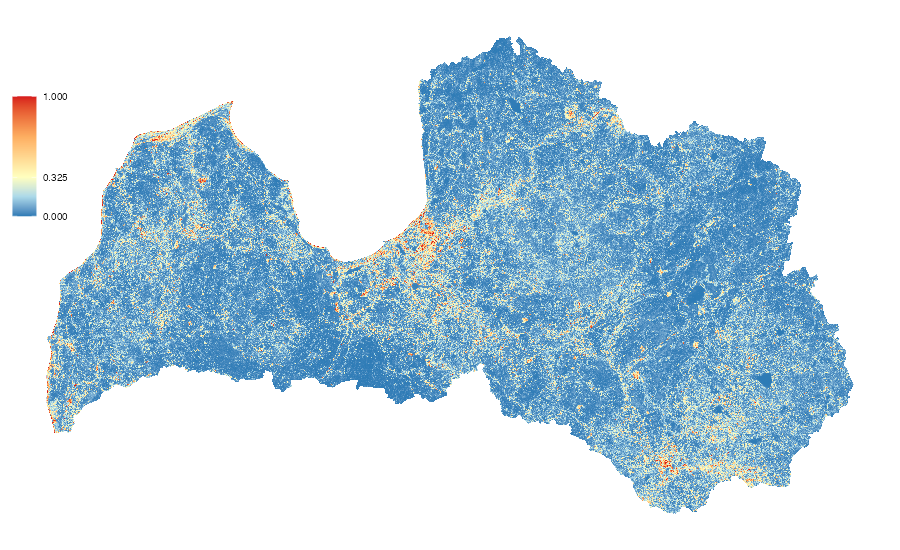
\includegraphics[width=1\linewidth,height=0.70\textheight,keepaspectratio]{results/LACAGIv2b/PicHSmap_LACAGI.png}

\par\small\textit{Predicted continuous habitat suitability across Latvia. The warmer the colour the higher is the predicted habitat suitability. Value in the middle of the legend correspond to the maximum training sensitivity plus specificity threshold. **For a full resolution refer to repository: link or online document: link**}\normalsize
\end{center}

\section*{Model thresholds}\label{model-thresholds-23}
\addcontentsline{toc}{section}{Model thresholds}

Threshold values and associated omission rates

\begin{center}
\resizebox{\linewidth}{!}{%

\begin{tabular}{lrrrrr}
\toprule
Threshold & Cloglog value & Fractional predicted area & Training omission rate & Test omission rate & P-values\\
\midrule
Minimum training presence & 0.0507050 & 0.7524894 & 0.0000000 & 0.0000982 & 0\\
Equal training sensitivity and specificity & 0.3713342 & 0.1859732 & 0.1865889 & 0.0022576 & 0\\
Maximum training sensitivity plus specificity & 0.3252916 & 0.2192645 & 0.1428571 & 0.0020612 & 0\\
Equal test sensitivity and specificity & 0.3780598 & 0.1818574 & 0.1953353 & 0.0022576 & 0\\
Maximum test sensitivity plus specificity & 0.3601674 & 0.1938396 & 0.1807580 & 0.0021594 & 0\\
\bottomrule
\end{tabular}
}
\end{center}

\section*{Variable importance}\label{variable-importance-23}
\addcontentsline{toc}{section}{Variable importance}

\begin{center}
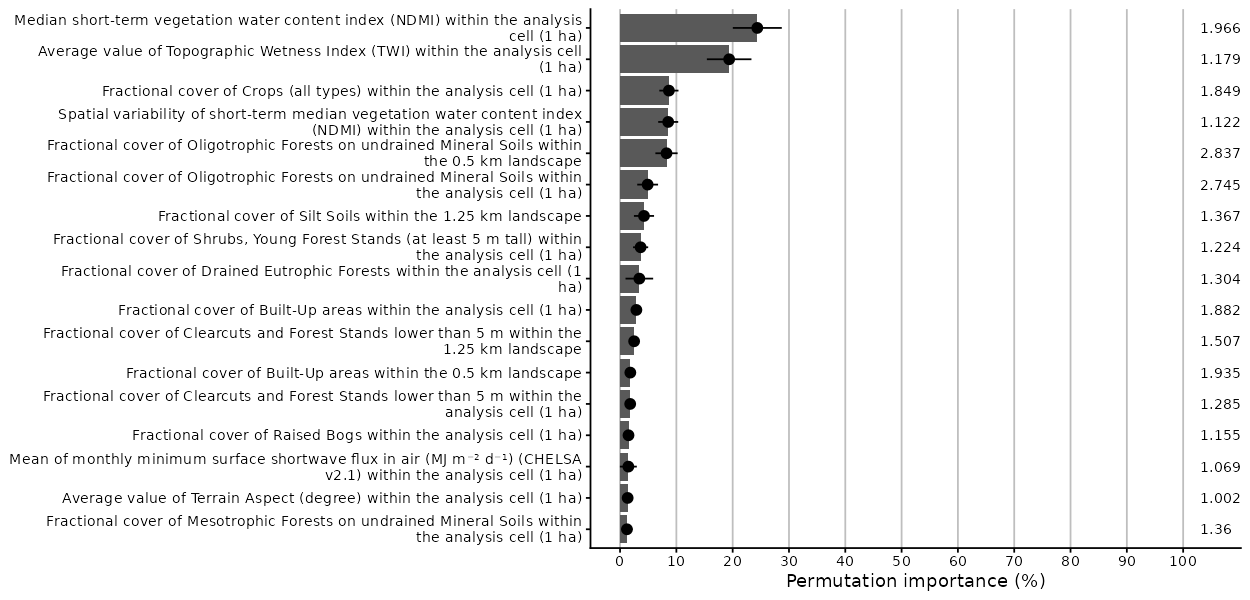
\includegraphics[width=1\linewidth,height=0.70\textheight,keepaspectratio]{results/LACAGIv2b/PicVarImpVIFs_LACAGI.png}

\par\small\textit{Permutation-importance (mean and standard deviation from 99 permutations, on the x-axis) of the ecogeographical variables (first y-axis, left side), and their variance inflation factor values (second y-axis, right side). **For a full resolution refer to repository: link or online document: link**}\normalsize
\end{center}

\section*{Marginal responses}\label{marginal-responses-23}
\addcontentsline{toc}{section}{Marginal responses}

\begin{center}
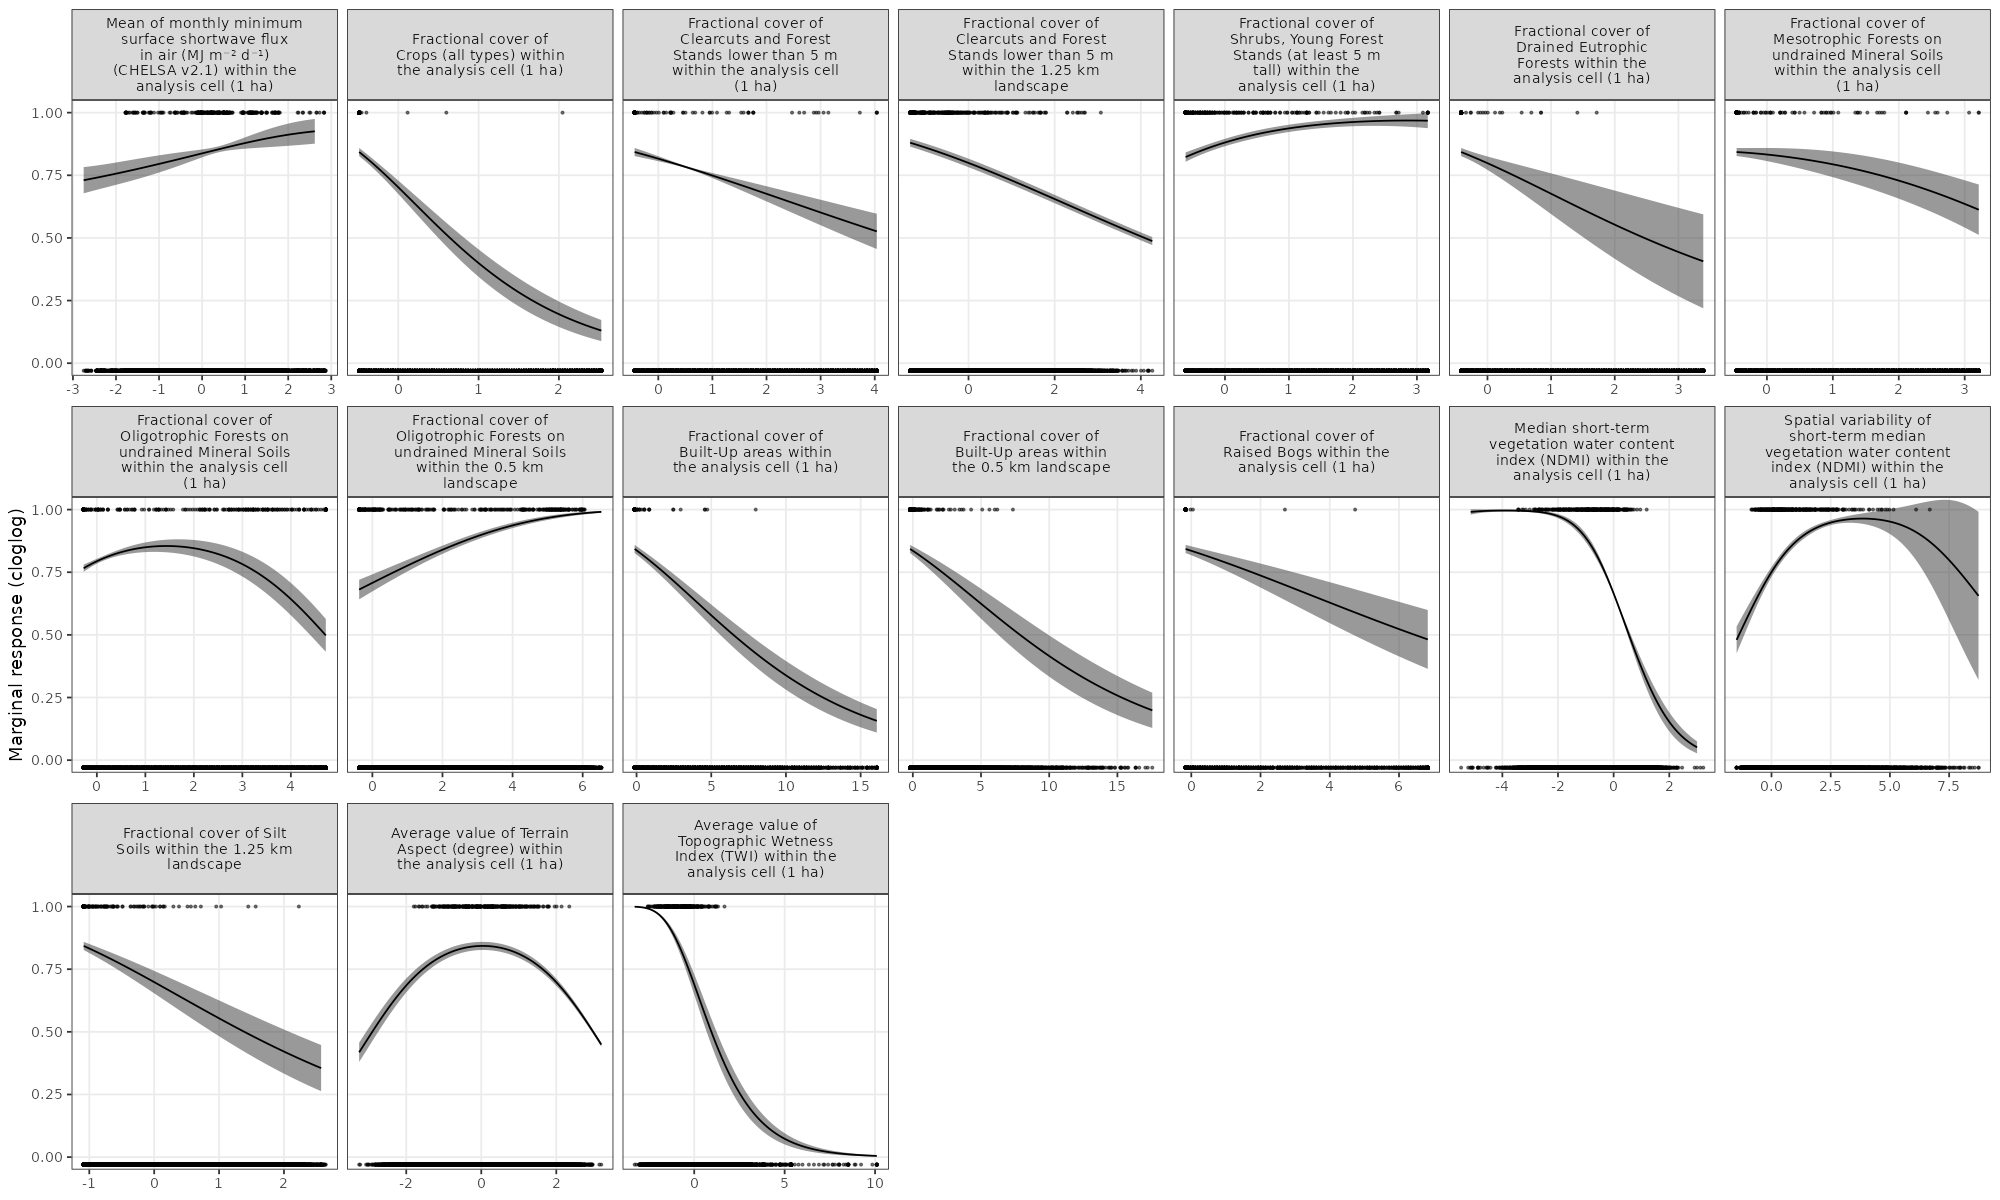
\includegraphics[width=1\linewidth,height=0.70\textheight,keepaspectratio]{results/LACAGIv2b/PicMargResp_LACAGI.png}

\par\small\textit{Marginalised for arithmetic mean response curves illustrating the effect of each ecogeographical variable on the habitat suitability when all the other variables have their arithmetic mean values. The y-axis shows the predicted habitat suitability (cloglog-transformed), while the x-axis shows the standardised (centred and scaled) value of the ecogeographical variable. Dots at a value of 1 on the y-axis illustrate presence locations in the environment (on the x-axis), while dots at a value of 0 illustrate background locations used in modelling.  **For a full resolution refer to repository: link or online document: link**}\normalsize
\end{center}

\section*{Habitat and conservation associations}\label{habitat-and-conservation-associations-23}
\addcontentsline{toc}{section}{Habitat and conservation associations}

\begin{center}
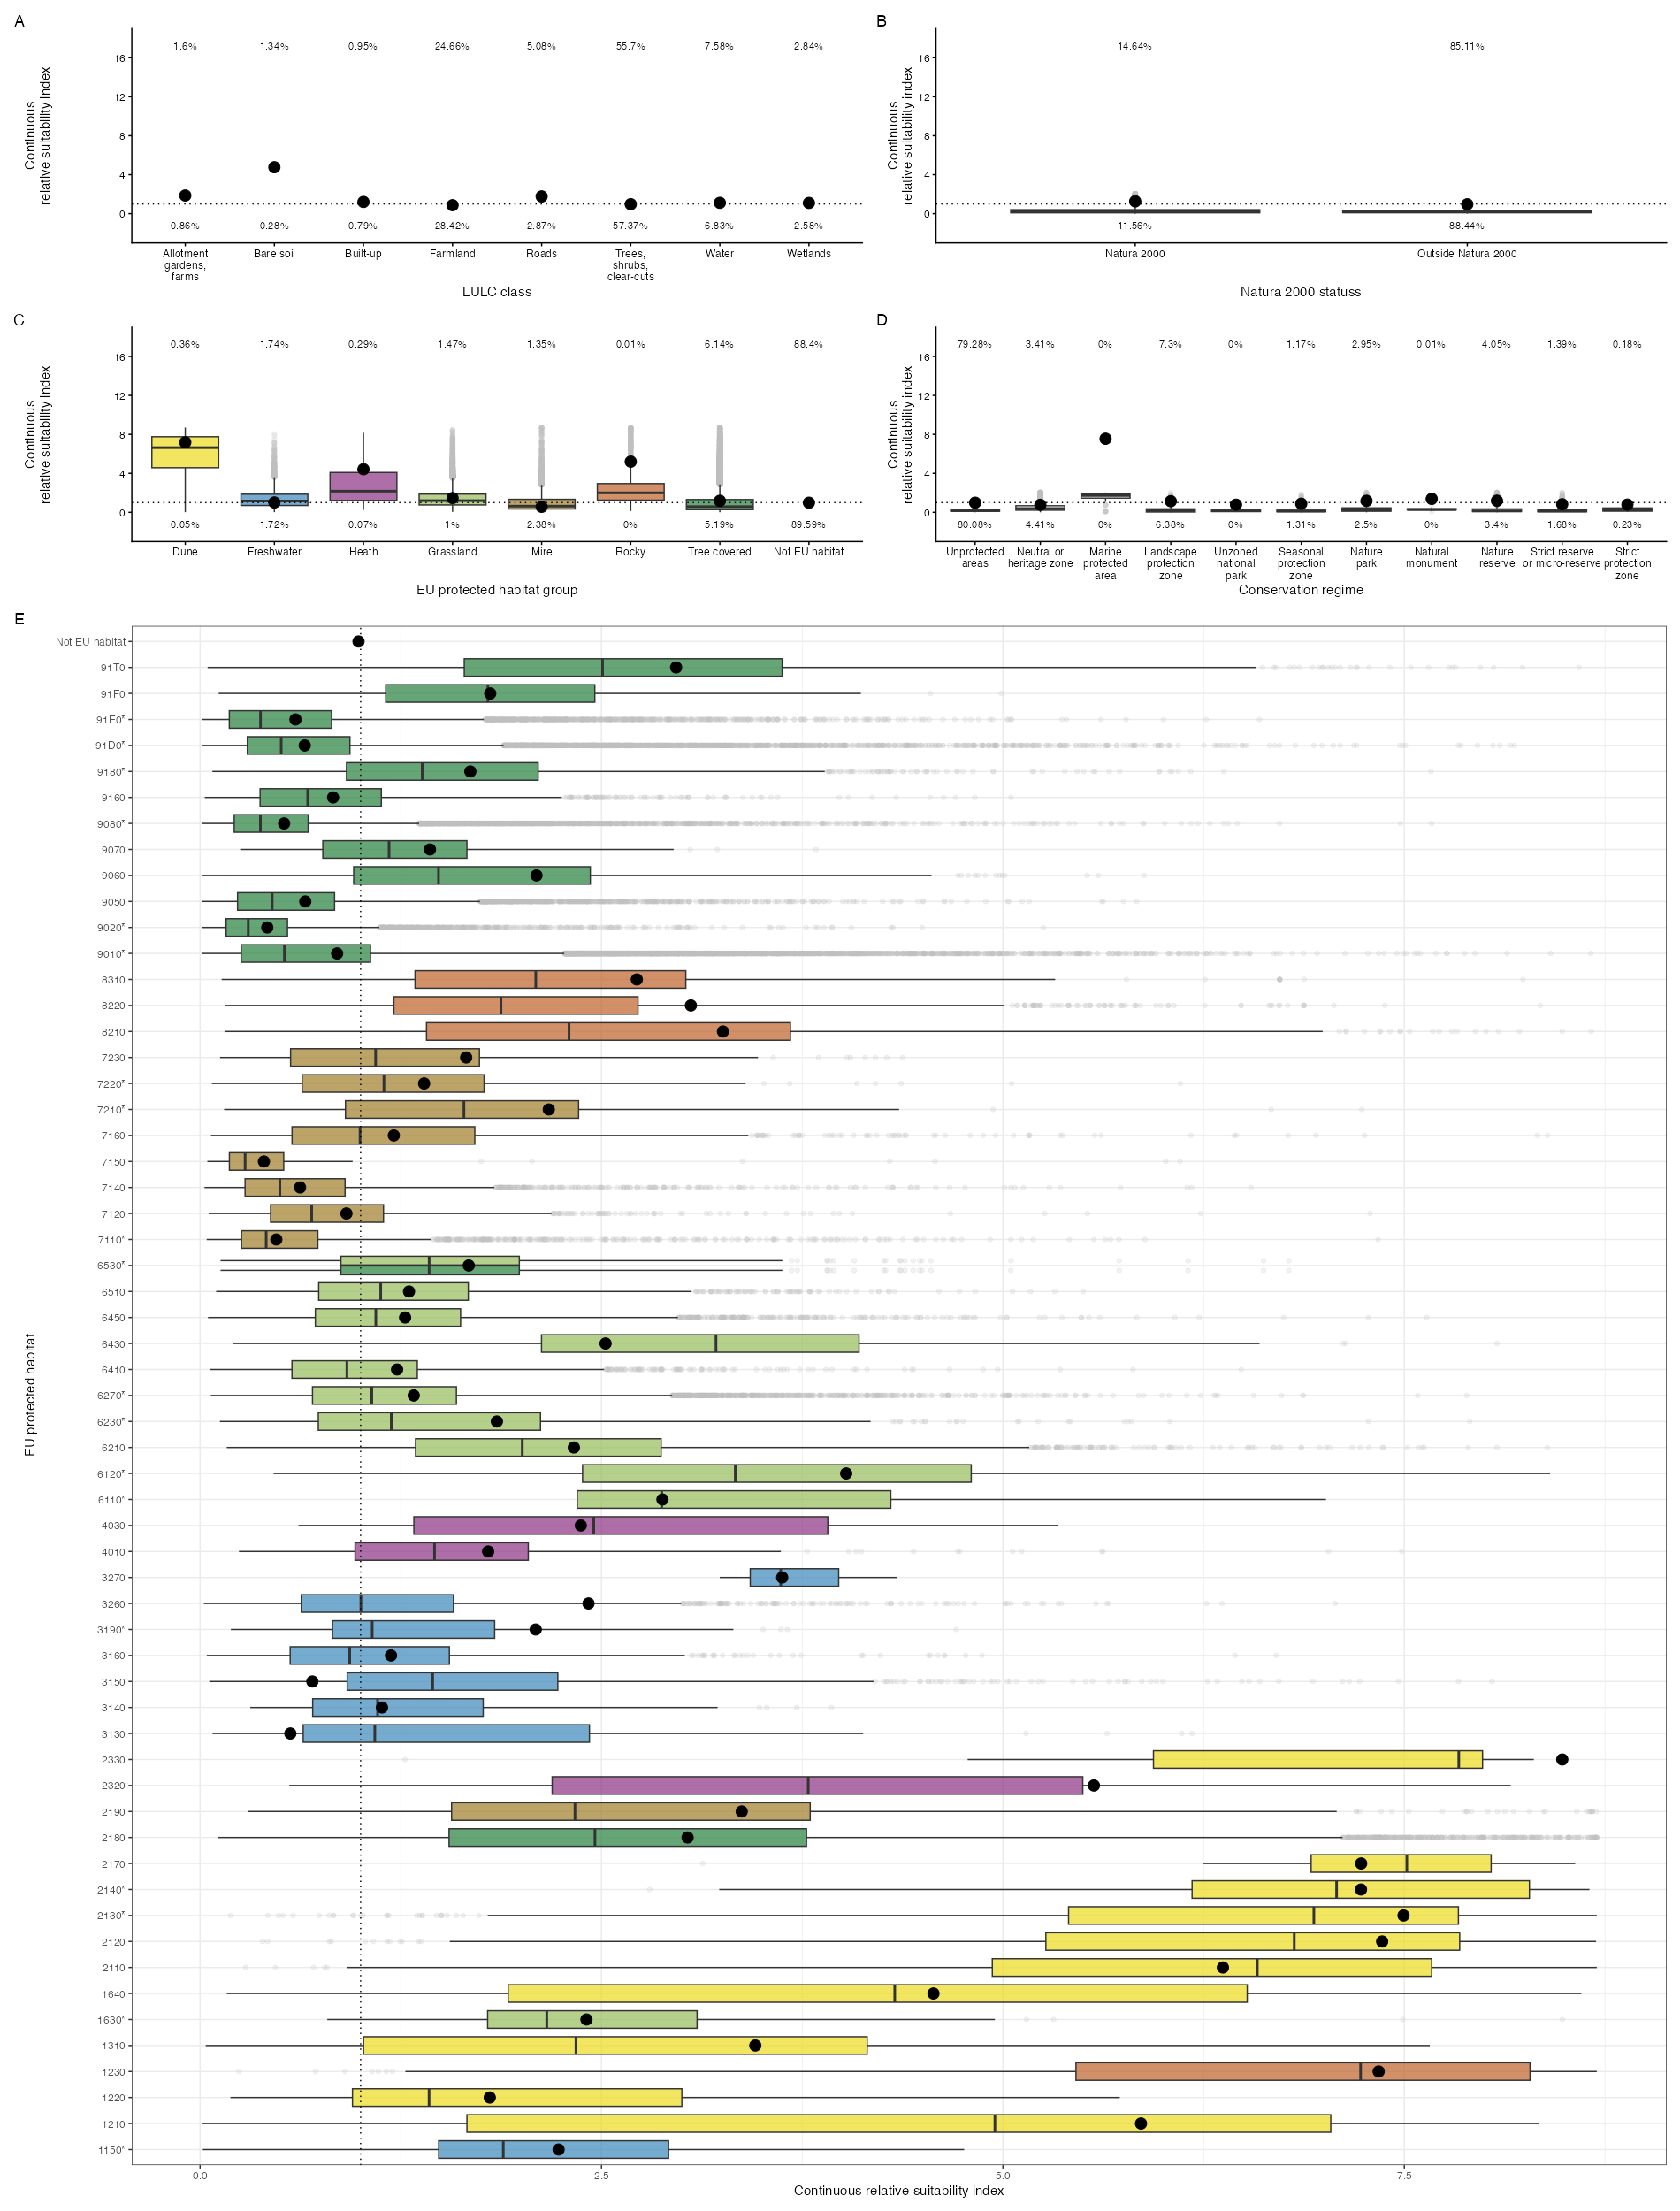
\includegraphics[width=1\linewidth,height=0.70\textheight,keepaspectratio]{results/LACAGIv2b/PicAssoc_LACAGI.png}

\par\small\textit{Associations between predicted suitability and: (A) land use land cover classes, (B) Natura 2000 status, (C) stratified EU protected habitat classes, (D) conservation regime, and (E) EU protected habitats. The y-axis show continuous relative suitability index (derivative of Manly's index of preference). Colours in (C) and (E) correspond to stratified EU protected habitat classes. For classifications composed of multiple individual polygons, polygon-level indices were additionally calculated to show within-category variation. The figures therefore combine category-level estimates (points) with the distributions of polygon-level values (boxplots, where applicable). Labels above and below the panels report, respectively, the percentage of total predicted suitability and the percentage of mapped area represented by each category. **For a full resolution refer to repository: link or online document: link**}\normalsize
\end{center}

\section*{Conservation prioritization}\label{conservation-prioritization-23}
\addcontentsline{toc}{section}{Conservation prioritization}

\begin{center}
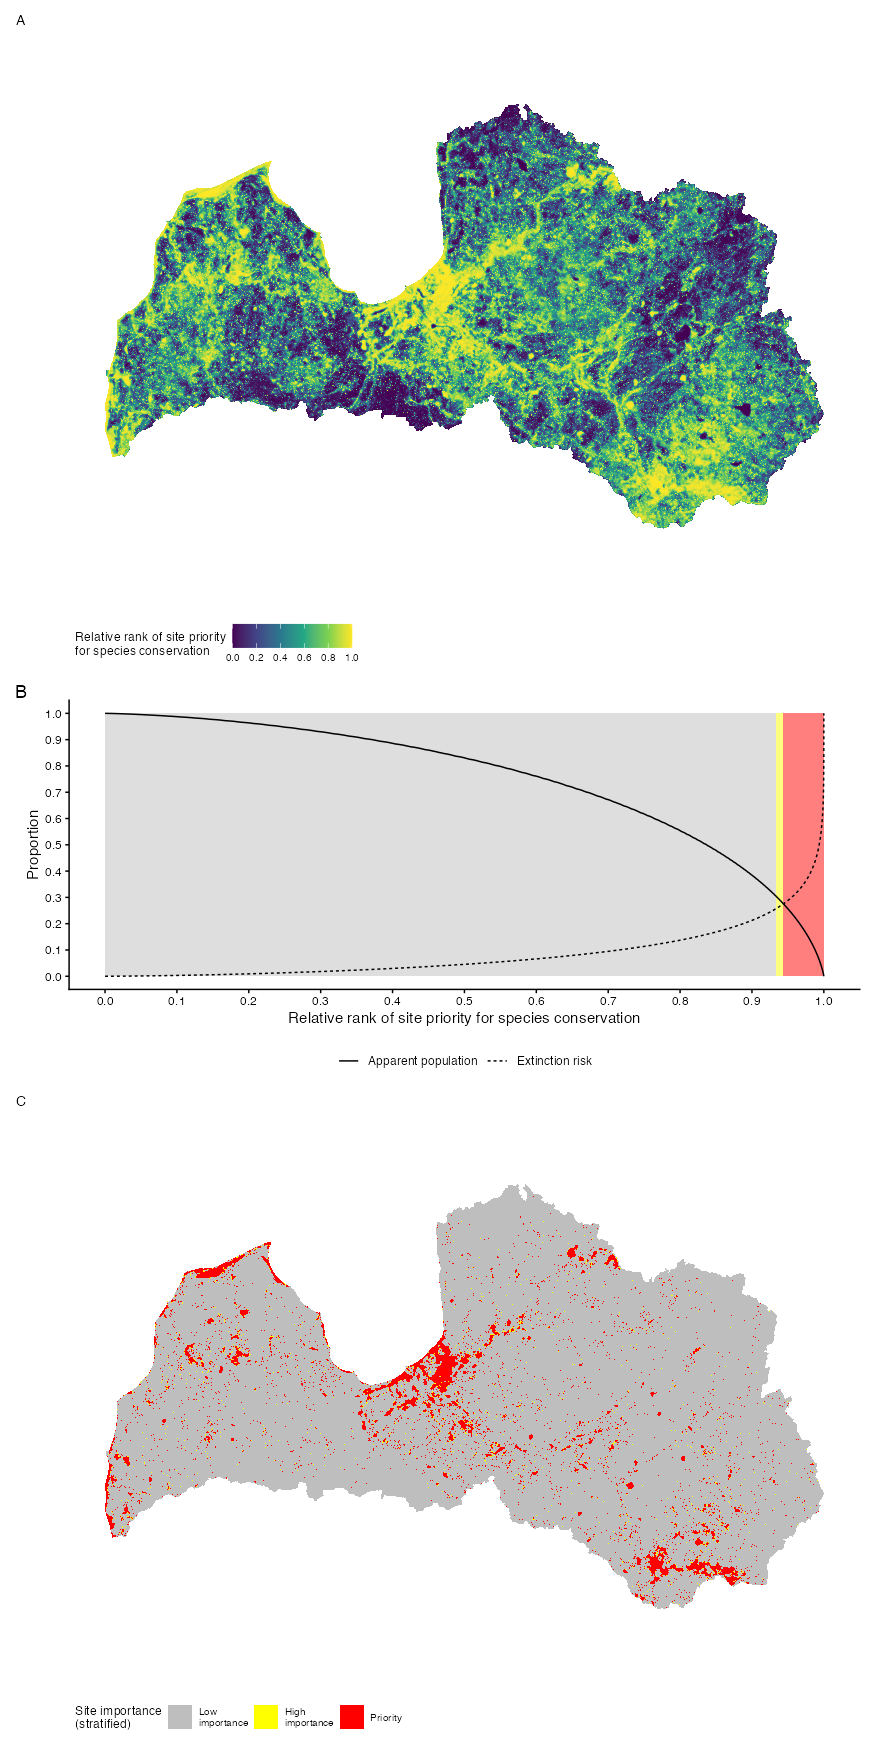
\includegraphics[width=0.85\linewidth,height=0.70\textheight,keepaspectratio]{results/LACAGIv2b/PicPrior_LACAGI.png}

\par\small\textit{Single-species conservation prioritization focusing on maximisation of core area protection (CAZMAX) while accounting for site connectivity: (A) relative site rank; (B) relationship between apparent-population and extinction-risk curves with a simplified classification which is spatially demonstrated in the bootom row; (C) spatial distribution of proposed classification of site prioritization results. **For a full resolution refer to repository: link or online document: link**}\normalsize
\end{center}

\chapter*{\texorpdfstring{\emph{Zootoca vivipara}}{Zootoca vivipara}}\label{zooviv}
\addcontentsline{toc}{chapter}{\emph{Zootoca vivipara}}

\section*{Summary}\label{summary-24}
\addcontentsline{toc}{section}{Summary}

\subsection*{Model description}\label{model-description-24}
\addcontentsline{toc}{subsection}{Model description}

Occurrence and background data were divided into model-training with four block spatial cross-validation data and an independent test set. Sampling-bias/background treatment: \textbf{Phenology Weighted Target Group}. Accumulated LULC change within the 1-ha analysis cell was not evaluated; accumulated LULC change within the home-range radius around the analysis cell was not evaluated.

The final data set contained \textbf{612} presence records: \textbf{459} for training with four spatial block cross-validation and \textbf{153} for independent testing. Training background contained \textbf{29997} locations, with \textbf{10003} additional independent-test background locations.

\subsection*{Expert assessment scores}\label{expert-assessment-scores-24}
\addcontentsline{toc}{subsection}{Expert assessment scores}

\begin{itemize}
\tightlist
\item
  \textbf{Marginal responses and variable importance score:} 4 (good ecological interpretability)
\item
  \textbf{Map score:} 5 (excellent agreement with known distribution)
\item
  \textbf{Applicability score:} 4 (high applicability)
\end{itemize}

\textbf{Šo sadaļu aizpildām manuāli no ekspertu aptaujām}

\subsection*{Statistical evaluation}\label{statistical-evaluation-24}
\addcontentsline{toc}{subsection}{Statistical evaluation}

The final model had a training TSS of \textbf{0.401}, with a training-derived cloglog threshold of \textbf{0.578}. Combined training AUC was \textbf{0.724} and combined test AUC was \textbf{0.71}.

\subsubsection*{Spatial cross-validation}\label{spatial-cross-validation-24}
\addcontentsline{toc}{subsubsection}{Spatial cross-validation}

\begin{itemize}
\tightlist
\item
  \textbf{AUC:} 0.6832 ± 0.0241; null models: 0.5062 ± 0.018; z = 9.8436, p \textless{} 0.001
\item
  \textbf{CBI:} 0.9478 ± 0.0172; null models: 0.0157 ± 0.156; z = 5.9759, p \textless{} 0.001
\item
  \textbf{OR10:} 0.1461 ± 0.044; null models: 0.188 ± 0.0584; z = -0.7174, p = 0.237
\item
  \textbf{ORmin:} 0.0044 ± 0.0088; null models: 0.0111 ± 0.0236; z = -0.2853, p = 0.388
\end{itemize}

\subsubsection*{Independent testing}\label{independent-testing-24}
\addcontentsline{toc}{subsubsection}{Independent testing}

\begin{itemize}
\tightlist
\item
  \textbf{TSS:} 0.352; \textbf{sensitivity:} 0.667; \textbf{specificity:} 0.685
\item
  \textbf{AUC:} 0.688; null models: 0.5067 ± 0.0479; z = 3.7778, p \textless{} 0.001
\item
  \textbf{CBI:} 0.923; null models: 0.0947 ± 0.5139; z = 1.6118, p = 0.054
\item
  \textbf{OR10:} 0.15; null models: 0.1273 ± 0.0487; z = 0.4724, p = 0.682
\item
  \textbf{ORmin:} 0.013; null models: 0.0032 ± 0.0067; z = 1.4663, p = 0.929
\end{itemize}

\subsection*{Conservation prioritisation summary}\label{conservation-prioritisation-summary-24}
\addcontentsline{toc}{subsection}{Conservation prioritisation summary}

The primary priority area covers \textbf{16.9\%} of Latvia and contains \textbf{27.6\%} of the summed habitat suitability (apparent population proxy).

The broader high importance area covers \textbf{30.8\%} of Latvia and contains \textbf{45.5\%} of the summed habitat suitability.

For comparison, the area classified as suitable using the maximum training sensitivity plus specificity habitat-suitability threshold contains \textbf{45.5\%} of the summed continuous habitat suitability.

\subsection*{Version evolution}\label{version-evolution-24}
\addcontentsline{toc}{subsection}{Version evolution}

\textbf{Šo sadaļu aizpildām manuāli, izmntojot sagatavotās shēmas. Jāvienojas par to noformējumu}

Describe model-version changes here. R chunks may be included in this block.

\section*{Habitat suitability}\label{habitat-suitability-24}
\addcontentsline{toc}{section}{Habitat suitability}

\begin{center}
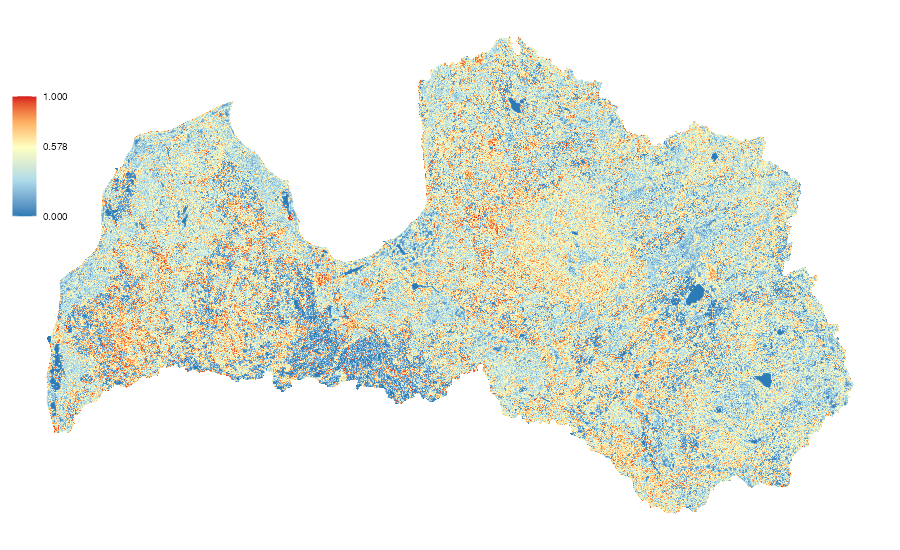
\includegraphics[width=1\linewidth,height=0.70\textheight,keepaspectratio]{results/ZOOVIVv3b1/PicHSmap_ZOOVIV.png}

\par\small\textit{Predicted continuous habitat suitability across Latvia. The warmer the colour the higher is the predicted habitat suitability. Value in the middle of the legend correspond to the maximum training sensitivity plus specificity threshold. **For a full resolution refer to repository: link or online document: link**}\normalsize
\end{center}

\section*{Model thresholds}\label{model-thresholds-24}
\addcontentsline{toc}{section}{Model thresholds}

Threshold values and associated omission rates

\begin{center}
\resizebox{\linewidth}{!}{%

\begin{tabular}{lrrrrr}
\toprule
Threshold & Cloglog value & Fractional predicted area & Training omission rate & Test omission rate & P-values\\
\midrule
Minimum training presence & 0.1017359 & 0.9704494 & 0.0000000 & 0.0000975 & 0\\
Equal training sensitivity and specificity & 0.5883871 & 0.3333443 & 0.3333333 & 0.0051672 & 0\\
Maximum training sensitivity plus specificity & 0.5784065 & 0.3482022 & 0.3093682 & 0.0049722 & 0\\
Equal test sensitivity and specificity & 0.5649963 & 0.3666259 & 0.3050109 & 0.0049722 & 0\\
Maximum test sensitivity plus specificity & 0.5835944 & 0.3402450 & 0.3289760 & 0.0049722 & 0\\
\bottomrule
\end{tabular}
}
\end{center}

\section*{Variable importance}\label{variable-importance-24}
\addcontentsline{toc}{section}{Variable importance}

\begin{center}
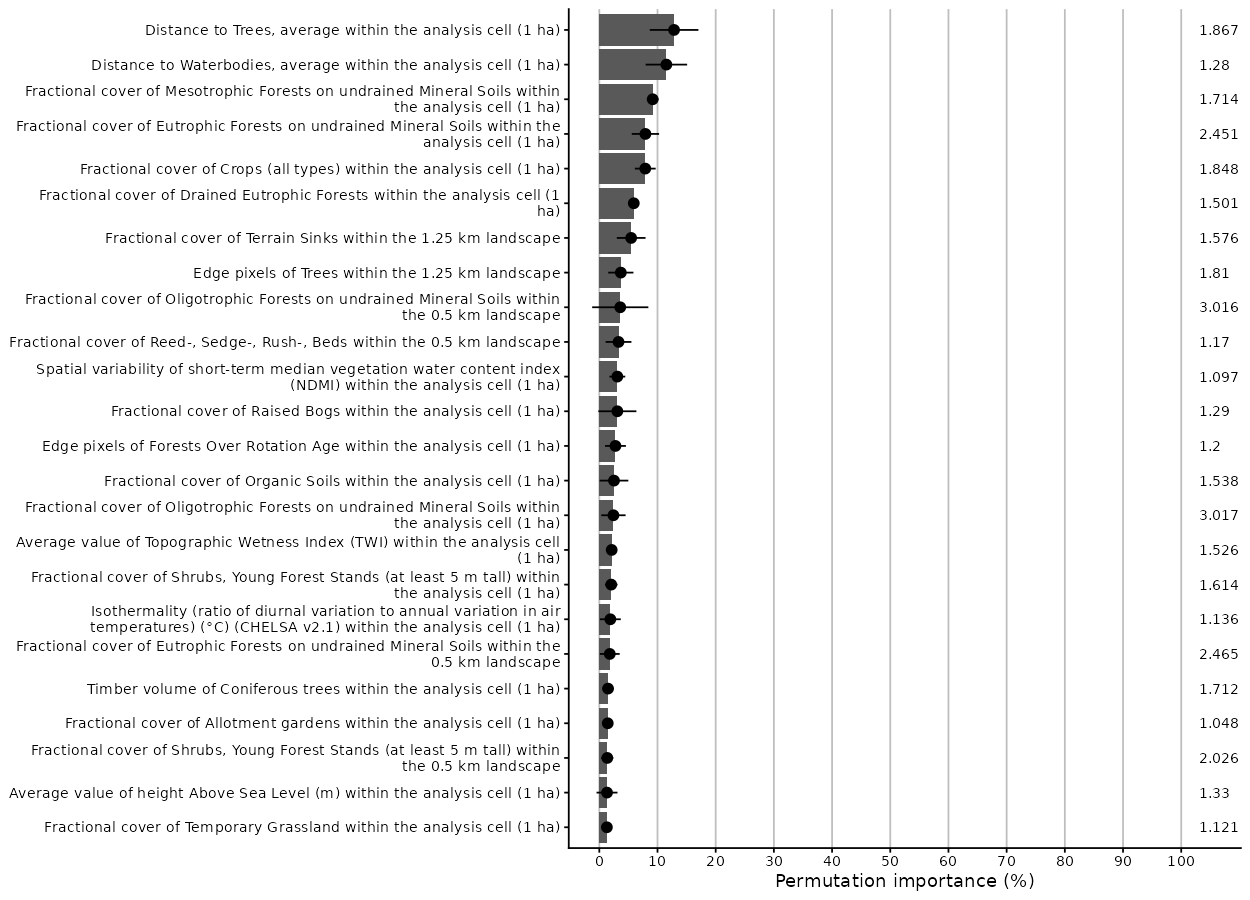
\includegraphics[width=1\linewidth,height=0.70\textheight,keepaspectratio]{results/ZOOVIVv3b1/PicVarImpVIFs_ZOOVIV.png}

\par\small\textit{Permutation-importance (mean and standard deviation from 99 permutations, on the x-axis) of the ecogeographical variables (first y-axis, left side), and their variance inflation factor values (second y-axis, right side). **For a full resolution refer to repository: link or online document: link**}\normalsize
\end{center}

\section*{Marginal responses}\label{marginal-responses-24}
\addcontentsline{toc}{section}{Marginal responses}

\begin{center}
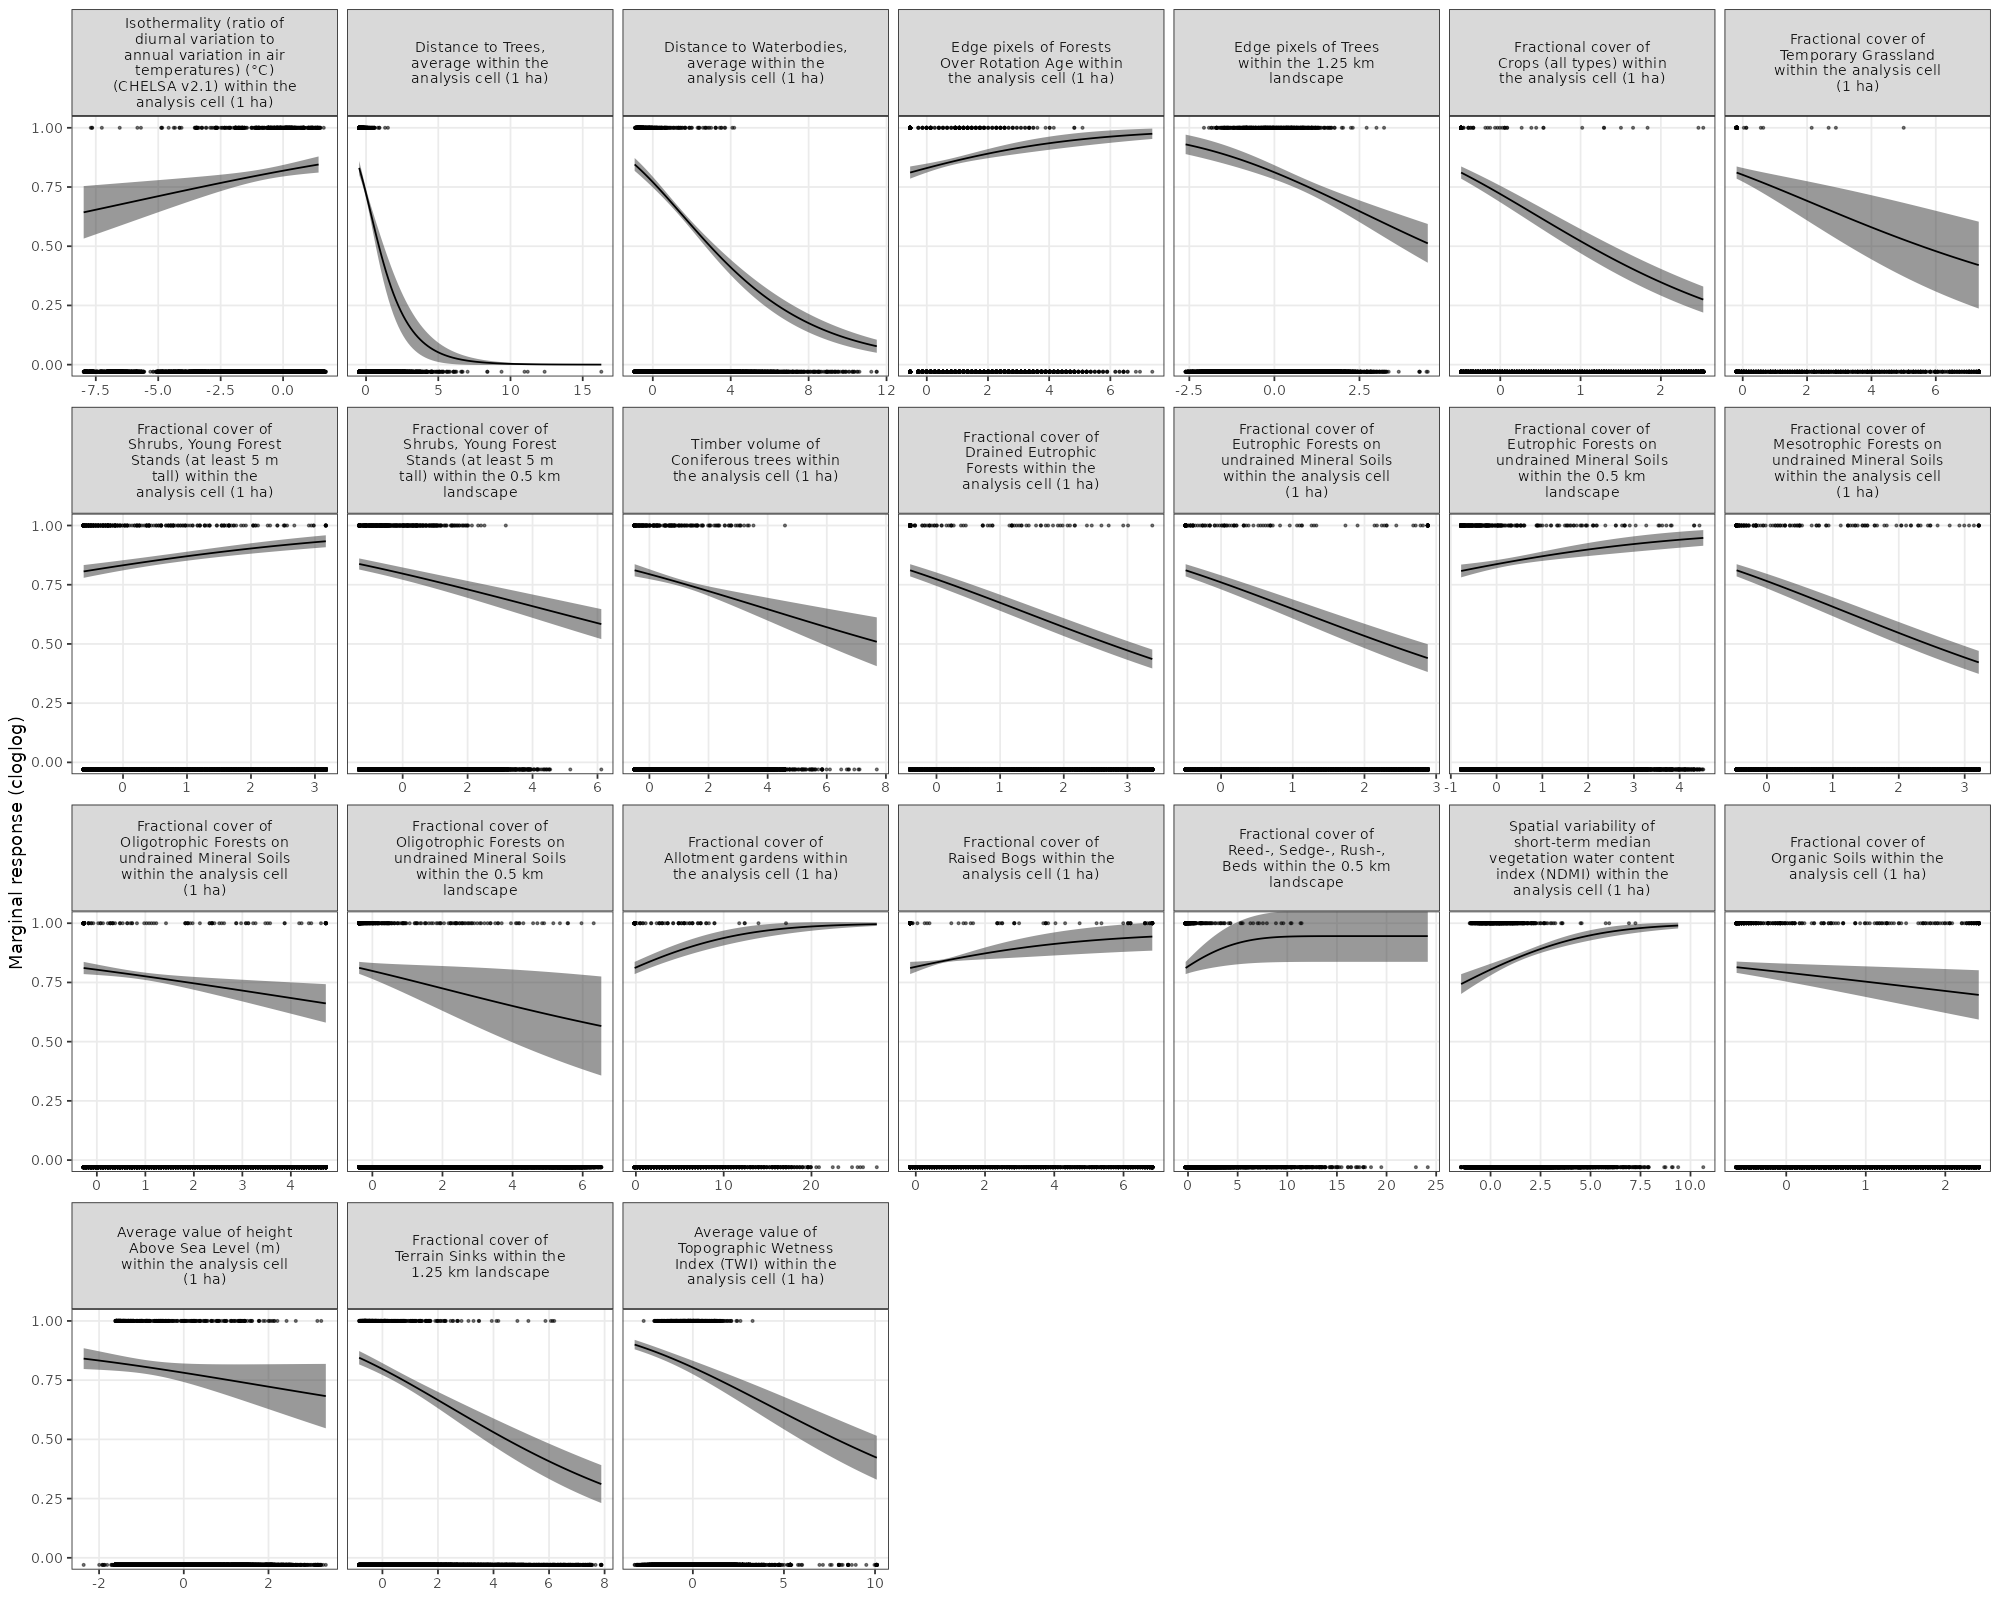
\includegraphics[width=1\linewidth,height=0.70\textheight,keepaspectratio]{results/ZOOVIVv3b1/PicMargResp_ZOOVIV.png}

\par\small\textit{Marginalised for arithmetic mean response curves illustrating the effect of each ecogeographical variable on the habitat suitability when all the other variables have their arithmetic mean values. The y-axis shows the predicted habitat suitability (cloglog-transformed), while the x-axis shows the standardised (centred and scaled) value of the ecogeographical variable. Dots at a value of 1 on the y-axis illustrate presence locations in the environment (on the x-axis), while dots at a value of 0 illustrate background locations used in modelling.  **For a full resolution refer to repository: link or online document: link**}\normalsize
\end{center}

\section*{Habitat and conservation associations}\label{habitat-and-conservation-associations-24}
\addcontentsline{toc}{section}{Habitat and conservation associations}

\begin{center}
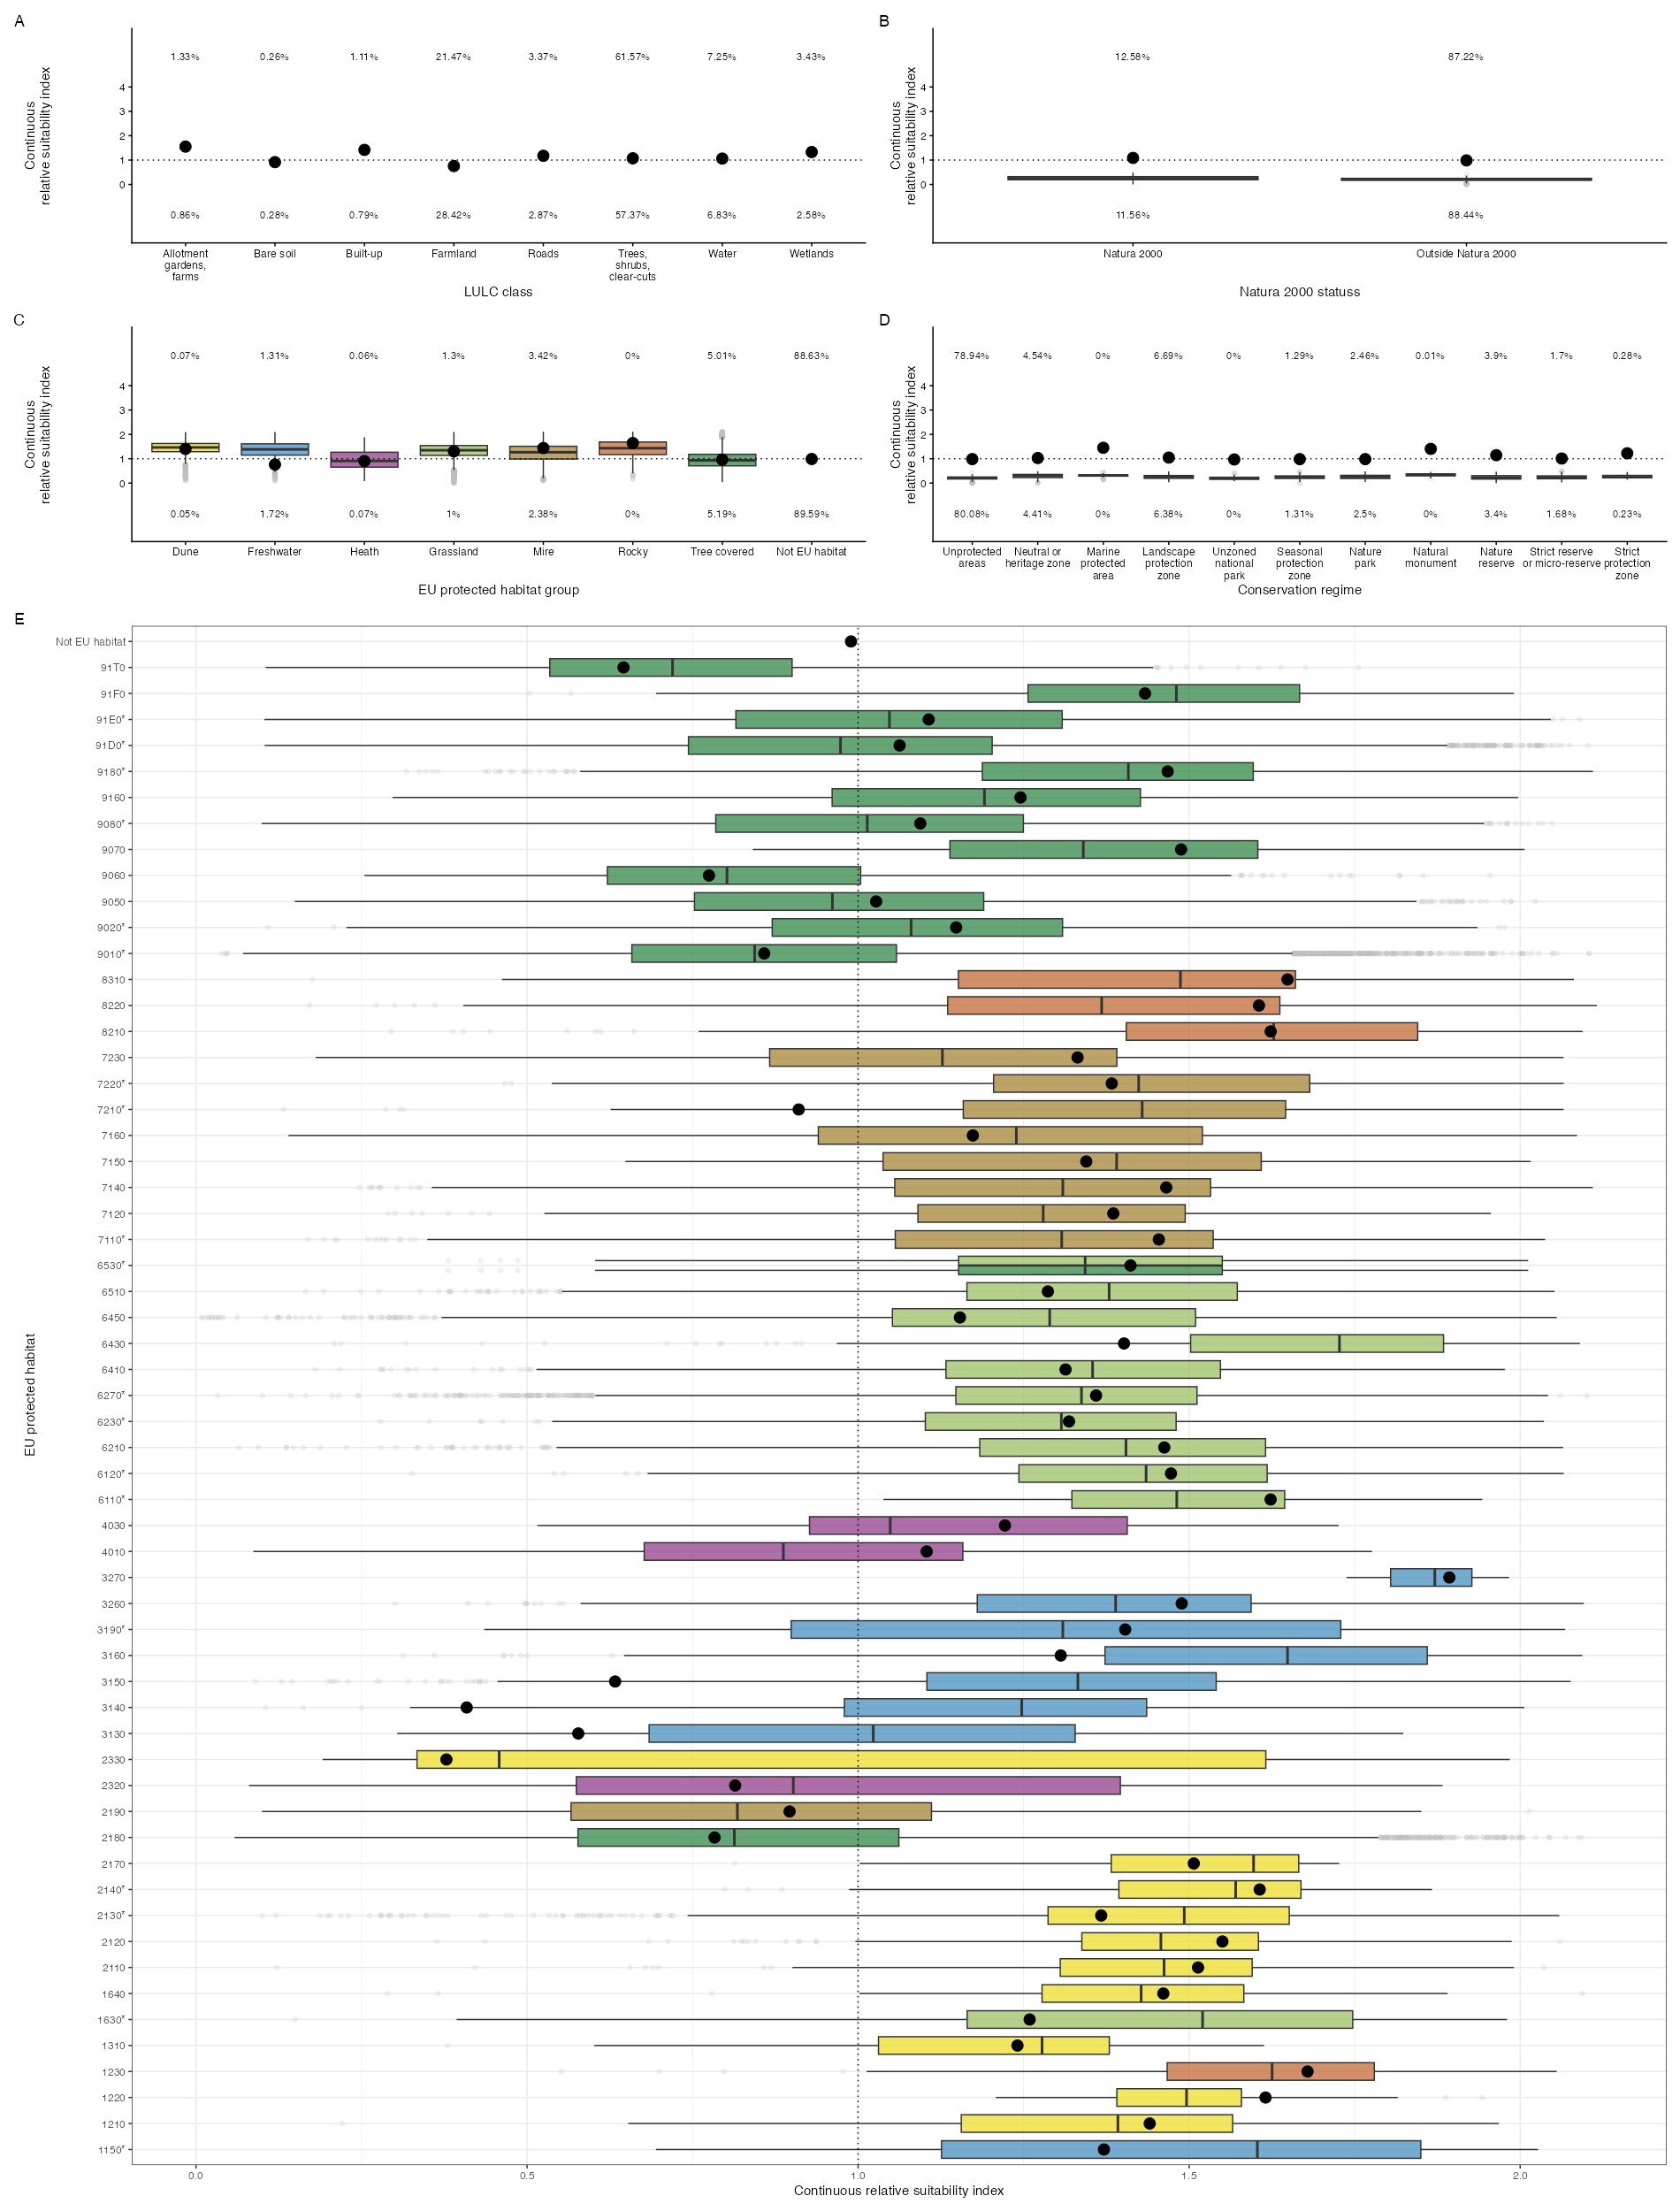
\includegraphics[width=1\linewidth,height=0.70\textheight,keepaspectratio]{results/ZOOVIVv3b1/PicAssoc_ZOOVIV.png}

\par\small\textit{Associations between predicted suitability and: (A) land use land cover classes, (B) Natura 2000 status, (C) stratified EU protected habitat classes, (D) conservation regime, and (E) EU protected habitats. The y-axis show continuous relative suitability index (derivative of Manly's index of preference). Colours in (C) and (E) correspond to stratified EU protected habitat classes. For classifications composed of multiple individual polygons, polygon-level indices were additionally calculated to show within-category variation. The figures therefore combine category-level estimates (points) with the distributions of polygon-level values (boxplots, where applicable). Labels above and below the panels report, respectively, the percentage of total predicted suitability and the percentage of mapped area represented by each category. **For a full resolution refer to repository: link or online document: link**}\normalsize
\end{center}

\section*{Conservation prioritization}\label{conservation-prioritization-24}
\addcontentsline{toc}{section}{Conservation prioritization}

\begin{center}
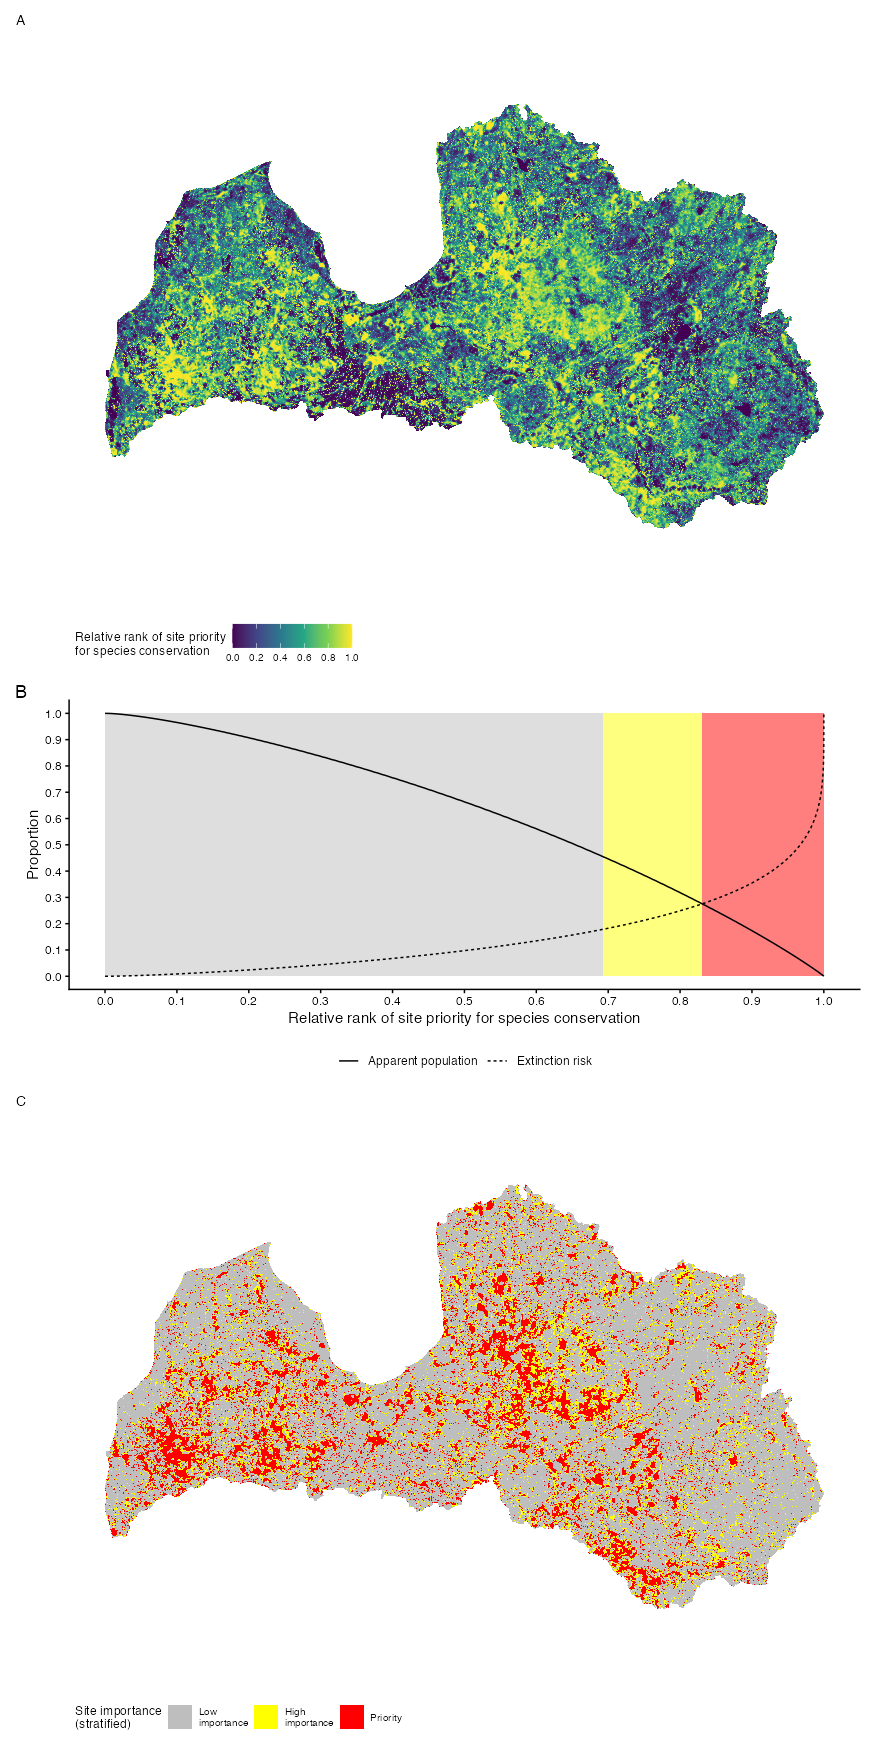
\includegraphics[width=0.85\linewidth,height=0.70\textheight,keepaspectratio]{results/ZOOVIVv3b1/PicPrior_ZOOVIV.png}

\par\small\textit{Single-species conservation prioritization focusing on maximisation of core area protection (CAZMAX) while accounting for site connectivity: (A) relative site rank; (B) relationship between apparent-population and extinction-risk curves with a simplified classification which is spatially demonstrated in the bootom row; (C) spatial distribution of proposed classification of site prioritization results. **For a full resolution refer to repository: link or online document: link**}\normalsize
\end{center}

\chapter*{\texorpdfstring{\emph{Coronella austriaca}}{Coronella austriaca}}\label{coraus}
\addcontentsline{toc}{chapter}{\emph{Coronella austriaca}}

\section*{Summary}\label{summary-25}
\addcontentsline{toc}{section}{Summary}

\subsection*{Model description}\label{model-description-25}
\addcontentsline{toc}{subsection}{Model description}

Occurrence and background data were used for model training with four block spatial cross-validation; no independent test split was used. Sampling-bias/background treatment: \textbf{Phenology Weighted Target Group}. Accumulated LULC change within the 1-ha analysis cell was not evaluated; accumulated LULC change within the home-range radius around the analysis cell was not evaluated.

The final data set contained \textbf{35} presence records: \textbf{35} for training with four spatial block cross-validation. Training background contained \textbf{40000} locations.

\subsection*{Expert assessment scores}\label{expert-assessment-scores-25}
\addcontentsline{toc}{subsection}{Expert assessment scores}

\begin{itemize}
\tightlist
\item
  \textbf{Marginal responses and variable importance score:} 4 (good ecological interpretability)
\item
  \textbf{Map score:} 5 (excellent agreement with known distribution)
\item
  \textbf{Applicability score:} 4 (high applicability)
\end{itemize}

\textbf{Šo sadaļu aizpildām manuāli no ekspertu aptaujām}

The model was considered ecologically plausible overall. Although the main
predictors showed relatively large uncertainty, no clearly uninterpretable
response relationships were identified. The habitat-suitability map agreed very
well with expert knowledge: known and field-tested locations were classified
appropriately, and no obviously implausible suitability patterns were evident.
Some small predicted hotspots occurred outside the currently known range, but
these were considered reasonable because the model included all known occurrences
while also identifying a plausible amount of potentially suitable habitat beyond
the presently documented distribution. The map was considered suitable for
species-conservation planning when used together with other ecological
information, while the explanatory value of the marginal response functions
was somewhat more limited.

Expert: Andris Čeirāns

\subsection*{Statistical evaluation}\label{statistical-evaluation-25}
\addcontentsline{toc}{subsection}{Statistical evaluation}

The final model had a training TSS of \textbf{0.401}, with a training-derived cloglog threshold of \textbf{0.362}. Combined training AUC was \textbf{0.989}.

\subsubsection*{Spatial cross-validation}\label{spatial-cross-validation-25}
\addcontentsline{toc}{subsubsection}{Spatial cross-validation}

\begin{itemize}
\tightlist
\item
  \textbf{AUC:} 0.9579 ± 0.0289; null models: 0.6483 ± 0.0801; z = 3.8648, p \textless{} 0.001
\item
  \textbf{CBI:} 0.7695 ± 0.1252; null models: 0.3264 ± 0.1826; z = 2.4268, p = 0.008
\item
  \textbf{OR10:} 0.4375 ± 0.2272; null models: 0.0953 ± 0.1487; z = 2.3006, p = 0.989
\item
  \textbf{ORmin:} 0.3229 ± 0.2209; null models: 0.0319 ± 0.109; z = 2.6699, p = 0.996
\end{itemize}

\subsection*{Conservation prioritisation summary}\label{conservation-prioritisation-summary-25}
\addcontentsline{toc}{subsection}{Conservation prioritisation summary}

The primary priority area covers \textbf{0.2\%} of Latvia and contains \textbf{27.5\%} of the summed habitat suitability (apparent population proxy).

For comparison, the area classified as suitable using the maximum training sensitivity plus specificity habitat-suitability threshold contains \textbf{24.6\%} of the summed continuous habitat suitability.

\subsection*{Version evolution}\label{version-evolution-25}
\addcontentsline{toc}{subsection}{Version evolution}

\textbf{Šo sadaļu aizpildām manuāli, izmntojot sagatavotās shēmas. Jāvienojas par to noformējumu}

The following diagram describes version evolution during modelling.
Colour codes:

\begin{itemize}
\item
  \textbf{black}: branch in version evolution from the initial EGV selection up
  until the best version;
\item
  \textbf{green}: the final version;
\item
  \textbf{grey}: other versions.
\end{itemize}

All the modifications on the black-to-green branch are described below the
diagram.

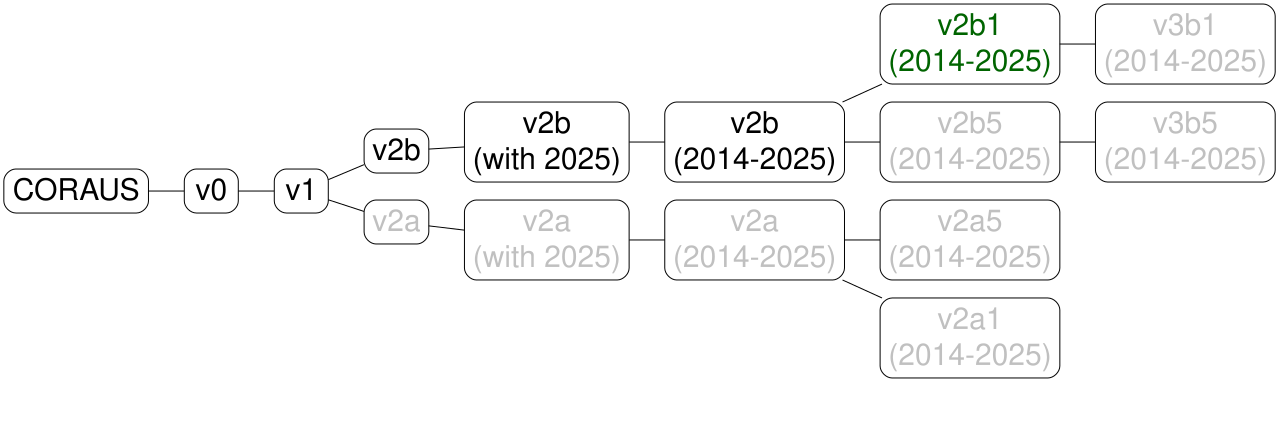
\includegraphics[width=1\linewidth]{figures/version_evolution/CORAUS_version_evolution}

\textbf{v0 to v1}

\begin{itemize}
\item
  EGVs excluded:

  \begin{itemize}
  \item
    egv\_150: (Edges\_Roads\_cell.tif) Edge pixels of Roads within the analysis cell (1 ha)
  \item
    egv\_423: (General\_ForestsWithoutInventory\_cell.tif) Fractional cover of Forests Without Inventory within the analysis cell (1 ha)
  \item
    egv\_424: (General\_ForestsWithoutInventory\_r500.tif) Fractional cover of Forests Without Inventory within the 0.5 km landscape
  \item
    egv\_425: (General\_ForestsWithoutInventory\_r1250.tif) Fractional cover of Forests Without Inventory within the 1.25 km landscape
  \item
    egv\_426: (General\_ForestsWithoutInventory\_r3000.tif) Fractional cover of Forests Without Inventory within the 3 km landscape
  \item
    egv\_427: (General\_ForestsWithoutInventory\_r10000.tif) Fractional cover of Forests Without Inventory within the 10 km landscape
  \item
    egv\_255: (FarmlandSubsidies\_BiologicalSubsidies\_cell.tif) Fractional cover of Farmland receiving Subsidies for Biological Agriculture within the analysis cell (1 ha)
  \item
    egv\_256: (FarmlandSubsidies\_BiologicalSubsidies\_r500.tif) Fractional cover of Farmland receiving Subsidies for Biological Agriculture within the 0.5 km landscape
  \item
    egv\_257: (FarmlandSubsidies\_BiologicalSubsidies\_r1250.tif) Fractional cover of Farmland receiving Subsidies for Biological Agriculture within the 1.25 km landscape
  \item
    egv\_258: (FarmlandSubsidies\_BiologicalSubsidies\_r3000.tif) Fractional cover of Farmland receiving Subsidies for Biological Agriculture within the 3 km landscape
  \item
    egv\_259: (FarmlandSubsidies\_BiologicalSubsidies\_r10000.tif) Fractional cover of Farmland receiving Subsidies for Biological Agriculture within the 10 km landscape
  \end{itemize}
\end{itemize}

\textbf{v1 to v2b}

\begin{itemize}
\item
  EGVs excluded:

  \begin{itemize}
  \tightlist
  \item
    egv\_093: (Distance\_Sea\_cell.tif) Distance to Sea, average within the analysis cell (1 ha)
  \end{itemize}
\item
  LULC change since the year of observation until the year 2024 are not used in
  observation filtering.
\end{itemize}

\textbf{v2b\_cv to v2b2025\_cv}

\begin{itemize}
\tightlist
\item
  occurence records from 2025 included in the presence data
\end{itemize}

\textbf{vb2025\_cv to v2b2014\_cv}

\begin{itemize}
\tightlist
\item
  occurence records from 2014-2015 included in the presence data
\end{itemize}

\textbf{v2b2014\_cv to v2b1\_2014\_cv}

\begin{itemize}
\item
  variable permutation importance ensured at at least 1\% if not affecting TSS
\item
  ensuring bottom limitation of the bias layer at 10\% of the layers global average
\end{itemize}

\section*{Habitat suitability}\label{habitat-suitability-25}
\addcontentsline{toc}{section}{Habitat suitability}

\begin{center}
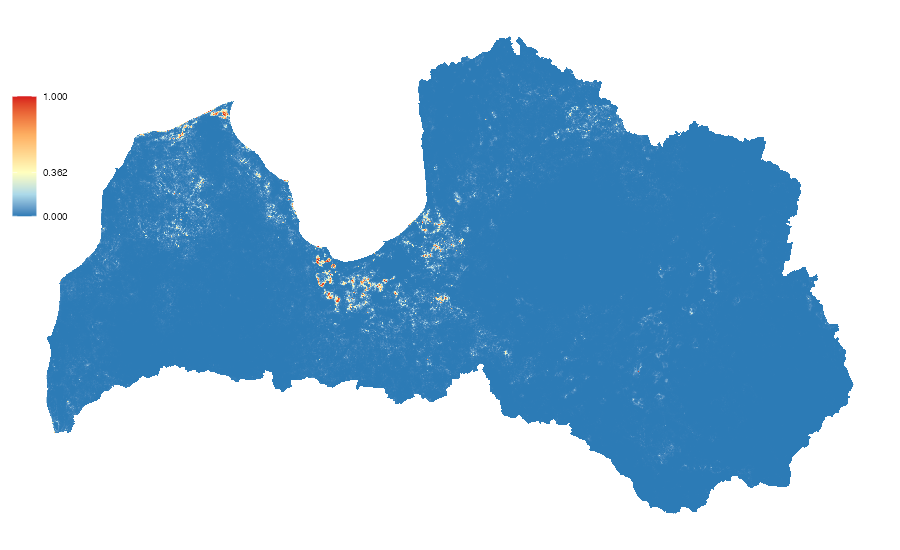
\includegraphics[width=1\linewidth,height=0.70\textheight,keepaspectratio]{results/CORAUSv2b1_2014_cv/PicHSmap_CORAUS.png}

\par\small\textit{Predicted continuous habitat suitability across Latvia. The warmer the colour the higher is the predicted habitat suitability. Value in the middle of the legend correspond to the maximum training sensitivity plus specificity threshold. **For a full resolution refer to repository: link or online document: link**}\normalsize
\end{center}

\section*{Model thresholds}\label{model-thresholds-25}
\addcontentsline{toc}{section}{Model thresholds}

Threshold values and associated omission rates

\begin{center}
\resizebox{\linewidth}{!}{%

\begin{tabular}{lrrr}
\toprule
Threshold & Cloglog value & Fractional predicted area & Training omission rate\\
\midrule
Minimum training presence & 0.3621532 & 0.048925 & 0.0000000\\
Equal training sensitivity and specificity & 0.3799319 & 0.047200 & 0.0571429\\
Maximum training sensitivity plus specificity & 0.3621532 & 0.048925 & 0.0000000\\
\bottomrule
\end{tabular}
}
\end{center}

\section*{Variable importance}\label{variable-importance-25}
\addcontentsline{toc}{section}{Variable importance}

\begin{center}
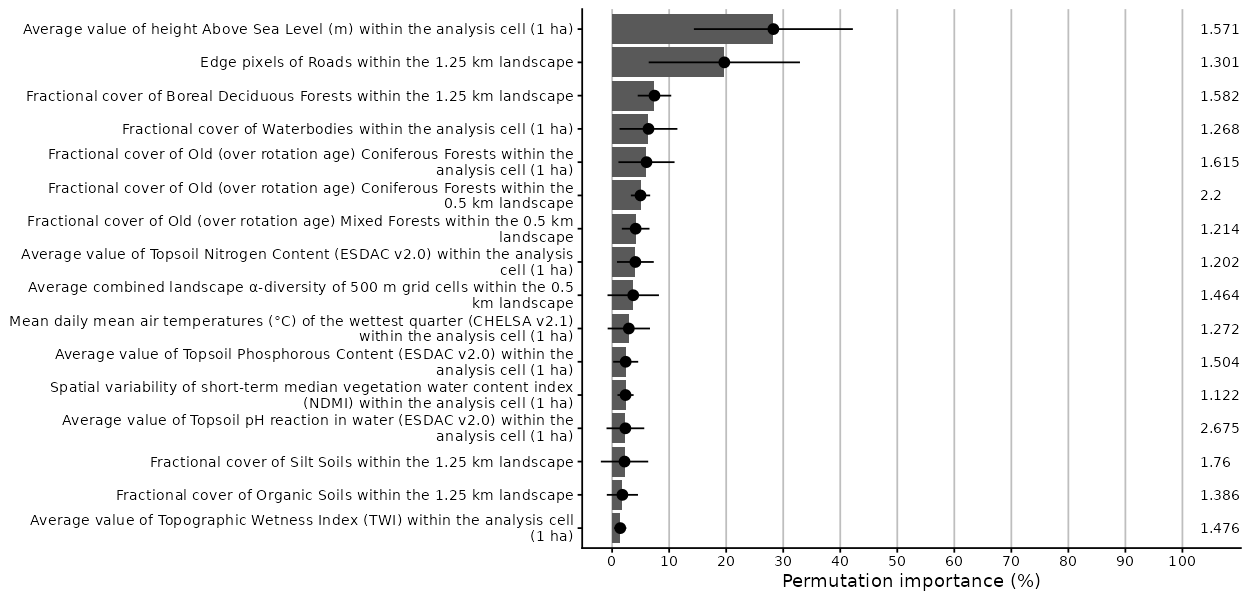
\includegraphics[width=1\linewidth,height=0.70\textheight,keepaspectratio]{results/CORAUSv2b1_2014_cv/PicVarImpVIFs_CORAUS.png}

\par\small\textit{Permutation-importance (mean and standard deviation from 99 permutations, on the x-axis) of the ecogeographical variables (first y-axis, left side), and their variance inflation factor values (second y-axis, right side). **For a full resolution refer to repository: link or online document: link**}\normalsize
\end{center}

\section*{Marginal responses}\label{marginal-responses-25}
\addcontentsline{toc}{section}{Marginal responses}

\begin{center}
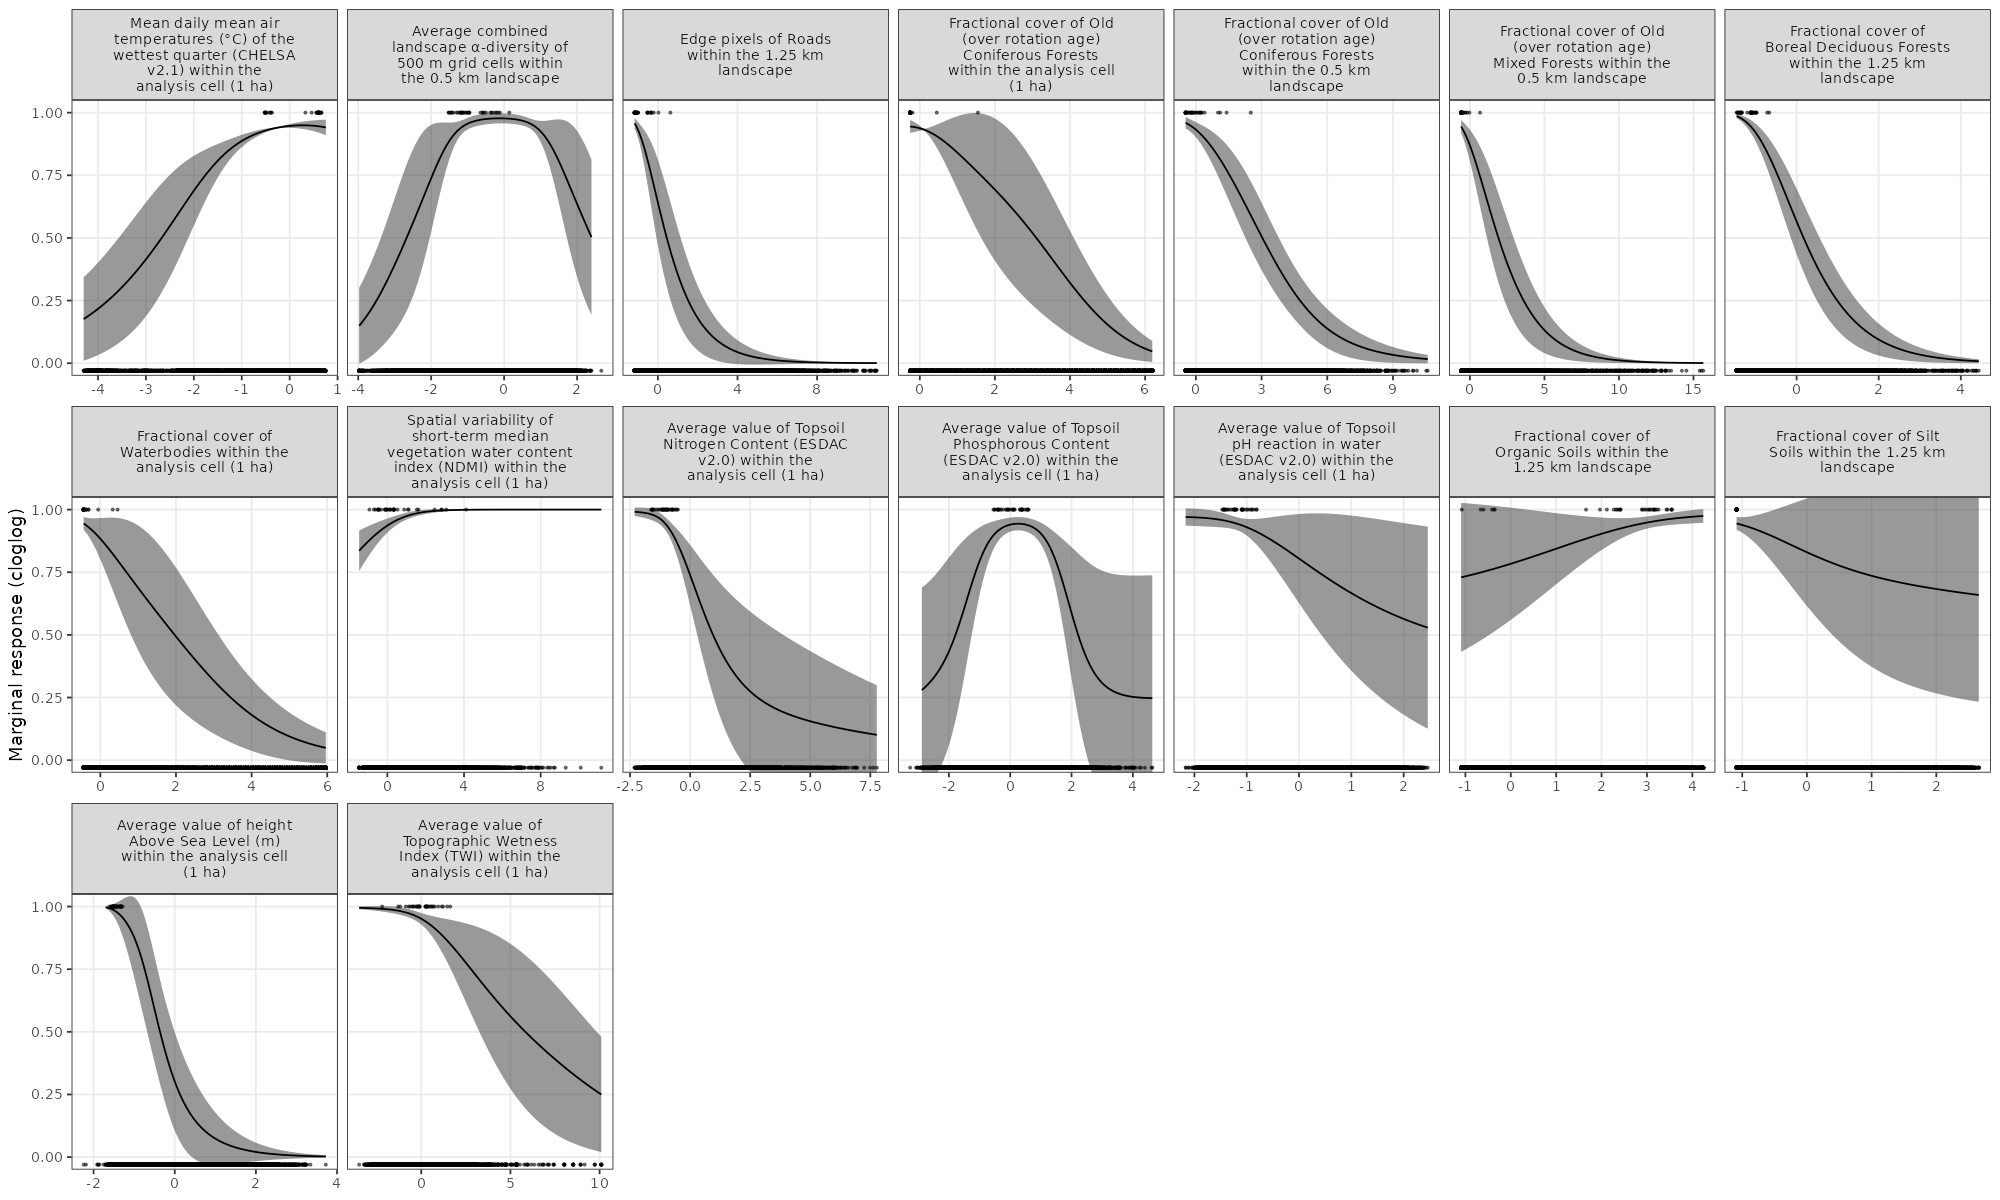
\includegraphics[width=1\linewidth,height=0.70\textheight,keepaspectratio]{results/CORAUSv2b1_2014_cv/PicMargResp_CORAUS.png}

\par\small\textit{Marginalised for arithmetic mean response curves illustrating the effect of each ecogeographical variable on the habitat suitability when all the other variables have their arithmetic mean values. The y-axis shows the predicted habitat suitability (cloglog-transformed), while the x-axis shows the standardised (centred and scaled) value of the ecogeographical variable. Dots at a value of 1 on the y-axis illustrate presence locations in the environment (on the x-axis), while dots at a value of 0 illustrate background locations used in modelling.  **For a full resolution refer to repository: link or online document: link**}\normalsize
\end{center}

\section*{Habitat and conservation associations}\label{habitat-and-conservation-associations-25}
\addcontentsline{toc}{section}{Habitat and conservation associations}

\begin{center}
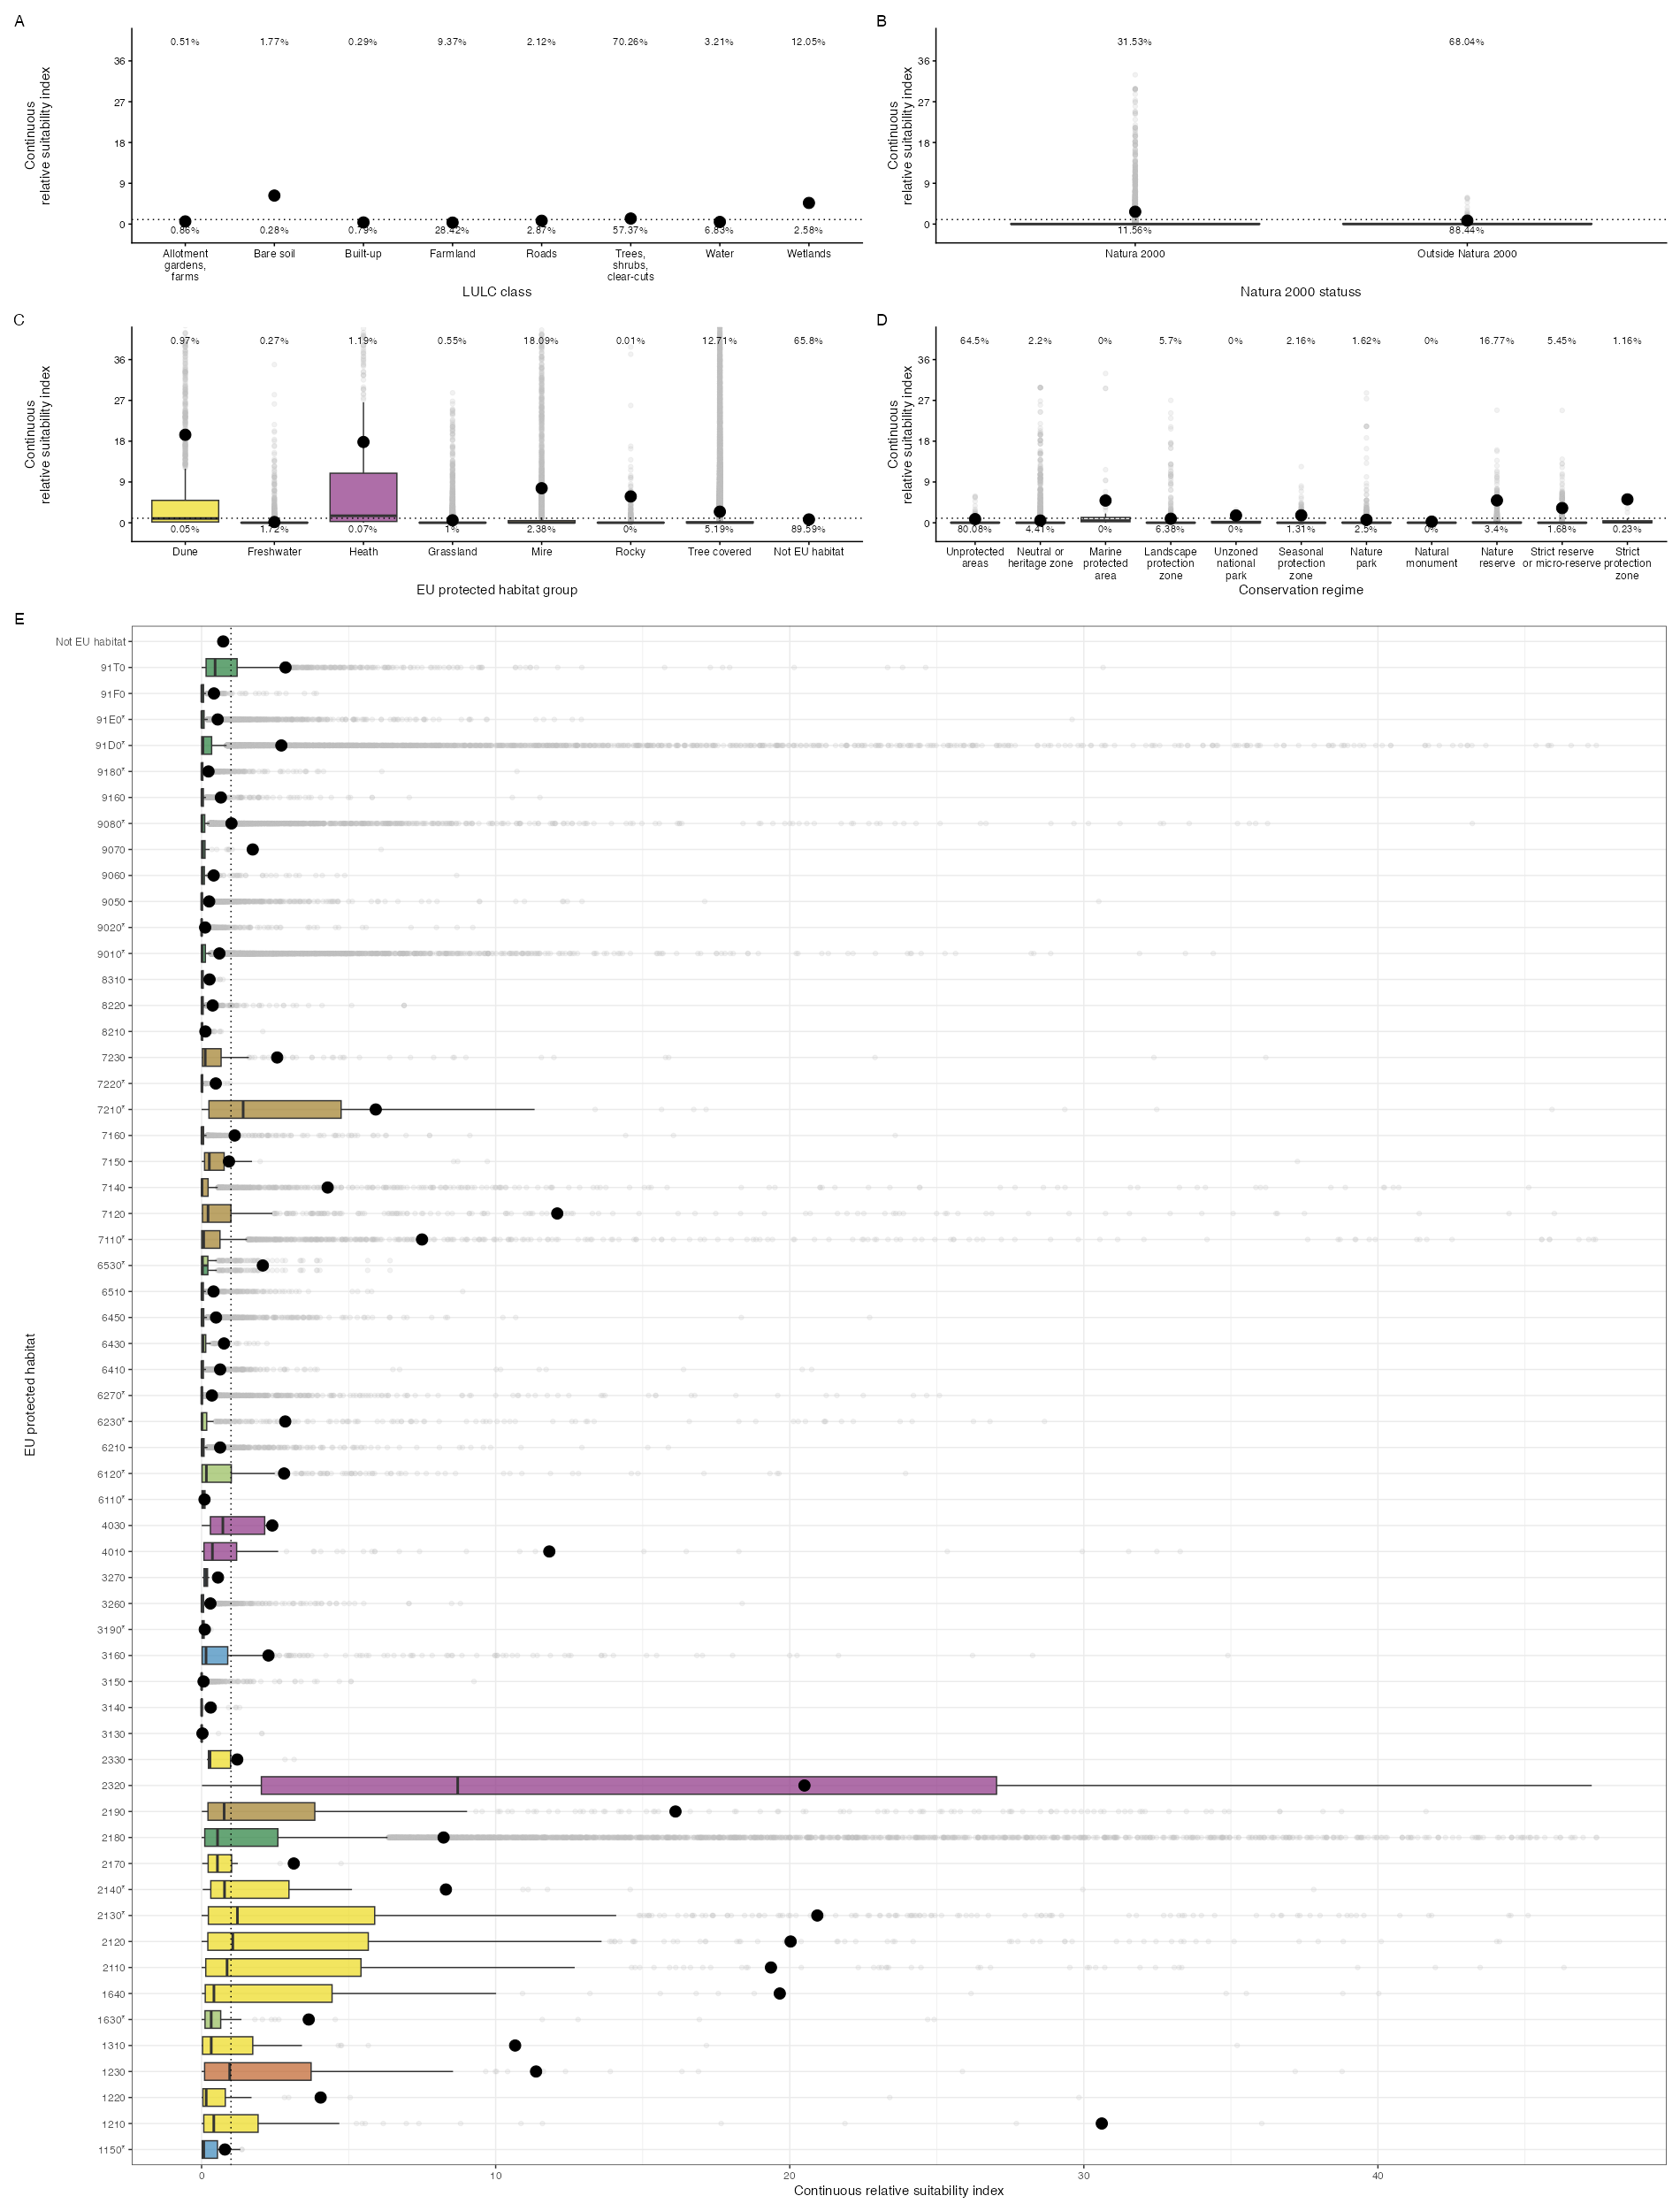
\includegraphics[width=1\linewidth,height=0.70\textheight,keepaspectratio]{results/CORAUSv2b1_2014_cv/PicAssoc_CORAUS.png}

\par\small\textit{Associations between predicted suitability and: (A) land use land cover classes, (B) Natura 2000 status, (C) stratified EU protected habitat classes, (D) conservation regime, and (E) EU protected habitats. The y-axis show continuous relative suitability index (derivative of Manly's index of preference). Colours in (C) and (E) correspond to stratified EU protected habitat classes. For classifications composed of multiple individual polygons, polygon-level indices were additionally calculated to show within-category variation. The figures therefore combine category-level estimates (points) with the distributions of polygon-level values (boxplots, where applicable). Labels above and below the panels report, respectively, the percentage of total predicted suitability and the percentage of mapped area represented by each category. **For a full resolution refer to repository: link or online document: link**}\normalsize
\end{center}

\section*{Conservation prioritization}\label{conservation-prioritization-25}
\addcontentsline{toc}{section}{Conservation prioritization}

\begin{center}
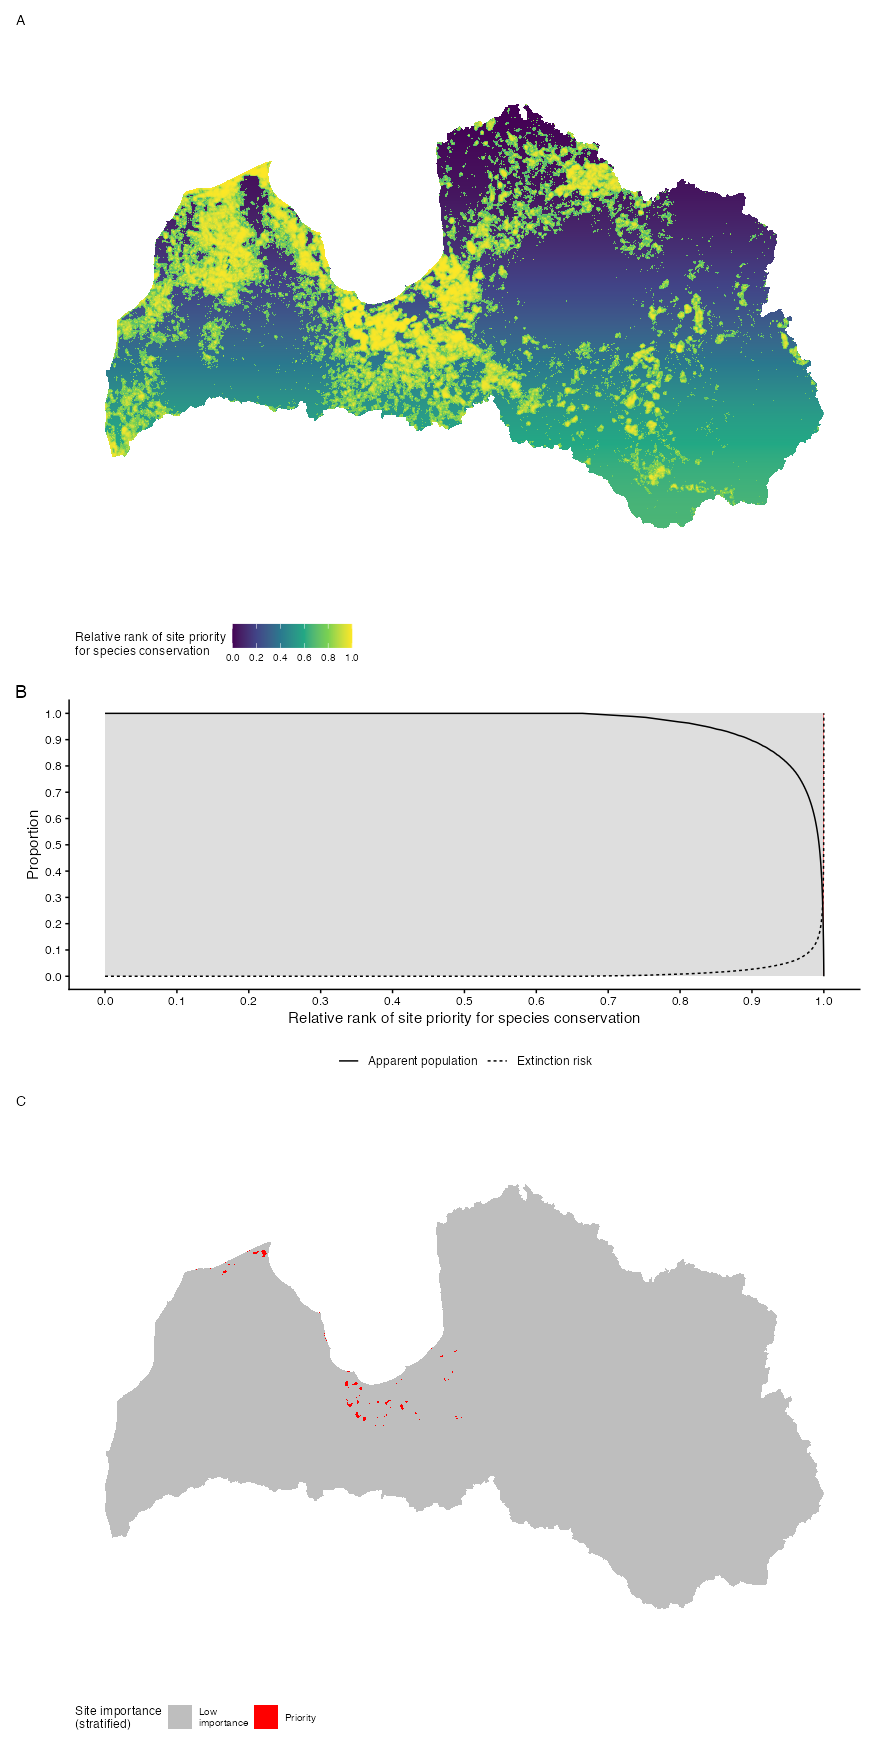
\includegraphics[width=0.85\linewidth,height=0.70\textheight,keepaspectratio]{results/CORAUSv2b1_2014_cv/PicPrior_CORAUS.png}

\par\small\textit{Single-species conservation prioritization focusing on maximisation of core area protection (CAZMAX) while accounting for site connectivity: (A) relative site rank; (B) relationship between apparent-population and extinction-risk curves with a simplified classification which is spatially demonstrated in the bootom row; (C) spatial distribution of proposed classification of site prioritization results. **For a full resolution refer to repository: link or online document: link**}\normalsize
\end{center}

\chapter*{\texorpdfstring{\emph{Natrix natrix}}{Natrix natrix}}\label{natnat}
\addcontentsline{toc}{chapter}{\emph{Natrix natrix}}

\section*{Summary}\label{summary-26}
\addcontentsline{toc}{section}{Summary}

\subsection*{Model description}\label{model-description-26}
\addcontentsline{toc}{subsection}{Model description}

Occurrence and background data were divided into model-training with four block spatial cross-validation data and an independent test set. Sampling-bias/background treatment: \textbf{Phenology Weighted Target Group}. Accumulated LULC change within the 1-ha analysis cell was not evaluated; accumulated LULC change within the home-range radius around the analysis cell was not evaluated.

The final data set contained \textbf{956} presence records: \textbf{722} for training with four spatial block cross-validation and \textbf{234} for independent testing. Training background contained \textbf{30042} locations, with \textbf{9958} additional independent-test background locations.

\subsection*{Expert assessment scores}\label{expert-assessment-scores-26}
\addcontentsline{toc}{subsection}{Expert assessment scores}

\begin{itemize}
\tightlist
\item
  \textbf{Marginal responses and variable importance score:} 4 (good ecological interpretability)
\item
  \textbf{Map score:} 3 (moderate agreement with known distribution)
\item
  \textbf{Applicability score:} 3 (moderate applicability)
\end{itemize}

\textbf{Šo sadaļu aizpildām manuāli no ekspertu aptaujām}

\subsection*{Statistical evaluation}\label{statistical-evaluation-26}
\addcontentsline{toc}{subsection}{Statistical evaluation}

The final model had a training TSS of \textbf{0.401}, with a training-derived cloglog threshold of \textbf{0.589}. Combined training AUC was \textbf{0.745} and combined test AUC was \textbf{0.694}.

\subsubsection*{Spatial cross-validation}\label{spatial-cross-validation-26}
\addcontentsline{toc}{subsubsection}{Spatial cross-validation}

\begin{itemize}
\tightlist
\item
  \textbf{AUC:} 0.7043 ± 0.0357; null models: 0.5312 ± 0.0212; z = 8.1529, p \textless{} 0.001
\item
  \textbf{CBI:} 0.9528 ± 0.0355; null models: 0.2531 ± 0.1702; z = 4.1106, p \textless{} 0.001
\item
  \textbf{OR10:} 0.1443 ± 0.0836; null models: 0.1029 ± 0.0515; z = 0.8044, p = 0.789
\item
  \textbf{ORmin:} 0.0014 ± 0.0028; null models: 0.0053 ± 0.0152; z = -0.2602, p = 0.397
\end{itemize}

\subsubsection*{Independent testing}\label{independent-testing-25}
\addcontentsline{toc}{subsubsection}{Independent testing}

\begin{itemize}
\tightlist
\item
  \textbf{TSS:} 0.258; \textbf{sensitivity:} 0.56; \textbf{specificity:} 0.698
\item
  \textbf{AUC:} 0.698; null models: 0.5204 ± 0.0613; z = 2.888, p = 0.002
\item
  \textbf{CBI:} 0.964; null models: 0.1498 ± 0.5159; z = 1.5782, p = 0.057
\item
  \textbf{OR10:} 0.137; null models: 0.0989 ± 0.0514; z = 0.7367, p = 0.769
\item
  \textbf{ORmin:} 0; null models: 9e-04 ± 0.0031; z = -0.2881, p = 0.387
\end{itemize}

\subsection*{Conservation prioritisation summary}\label{conservation-prioritisation-summary-26}
\addcontentsline{toc}{subsection}{Conservation prioritisation summary}

The primary priority area covers \textbf{16\%} of Latvia and contains \textbf{27.6\%} of the summed habitat suitability (apparent population proxy).

The broader high importance area covers \textbf{20.9\%} of Latvia and contains \textbf{34.5\%} of the summed habitat suitability.

For comparison, the area classified as suitable using the maximum training sensitivity plus specificity habitat-suitability threshold contains \textbf{34.5\%} of the summed continuous habitat suitability.

\subsection*{Version evolution}\label{version-evolution-26}
\addcontentsline{toc}{subsection}{Version evolution}

\textbf{Šo sadaļu aizpildām manuāli, izmntojot sagatavotās shēmas. Jāvienojas par to noformējumu}

\section*{Habitat suitability}\label{habitat-suitability-26}
\addcontentsline{toc}{section}{Habitat suitability}

\begin{center}
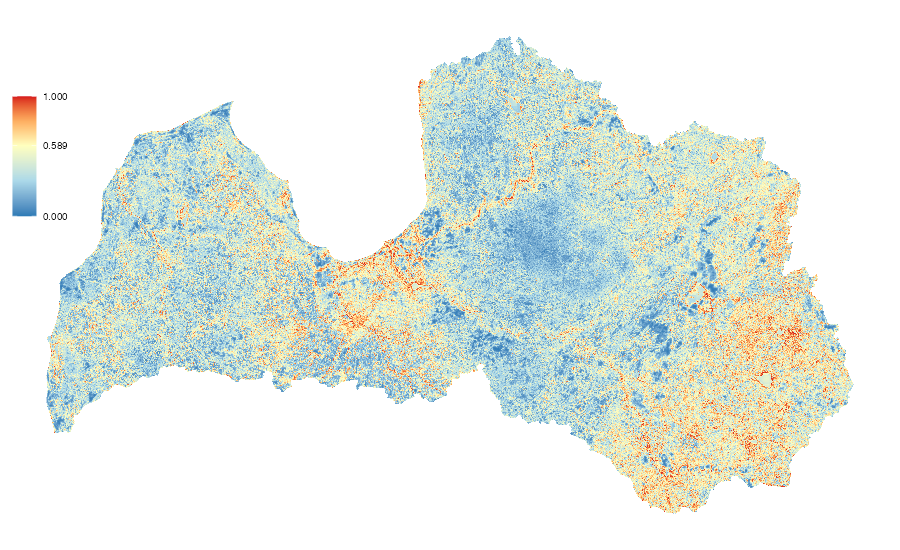
\includegraphics[width=1\linewidth,height=0.70\textheight,keepaspectratio]{results/NATNATv2b/PicHSmap_NATNAT.png}

\par\small\textit{Predicted continuous habitat suitability across Latvia. The warmer the colour the higher is the predicted habitat suitability. Value in the middle of the legend correspond to the maximum training sensitivity plus specificity threshold. **For a full resolution refer to repository: link or online document: link**}\normalsize
\end{center}

\section*{Model thresholds}\label{model-thresholds-26}
\addcontentsline{toc}{section}{Model thresholds}

Threshold values and associated omission rates

\begin{center}
\resizebox{\linewidth}{!}{%

\begin{tabular}{lrrrrr}
\toprule
Threshold & Cloglog value & Fractional predicted area & Training omission rate & Test omission rate & P-values\\
\midrule
Minimum training presence & 0.0405788 & 0.9937797 & 0.0000000 & 0.0000000 & 0\\
Equal training sensitivity and specificity & 0.5680384 & 0.3227042 & 0.3227147 & 0.0093675 & 0\\
Maximum training sensitivity plus specificity & 0.5887348 & 0.2941234 & 0.3448753 & 0.0099469 & 0\\
Equal test sensitivity and specificity & 0.5457872 & 0.3537731 & 0.2908587 & 0.0082086 & 0\\
Maximum test sensitivity plus specificity & 0.4660602 & 0.4752987 & 0.1994460 & 0.0047320 & 0\\
\bottomrule
\end{tabular}
}
\end{center}

\section*{Variable importance}\label{variable-importance-26}
\addcontentsline{toc}{section}{Variable importance}

\begin{center}
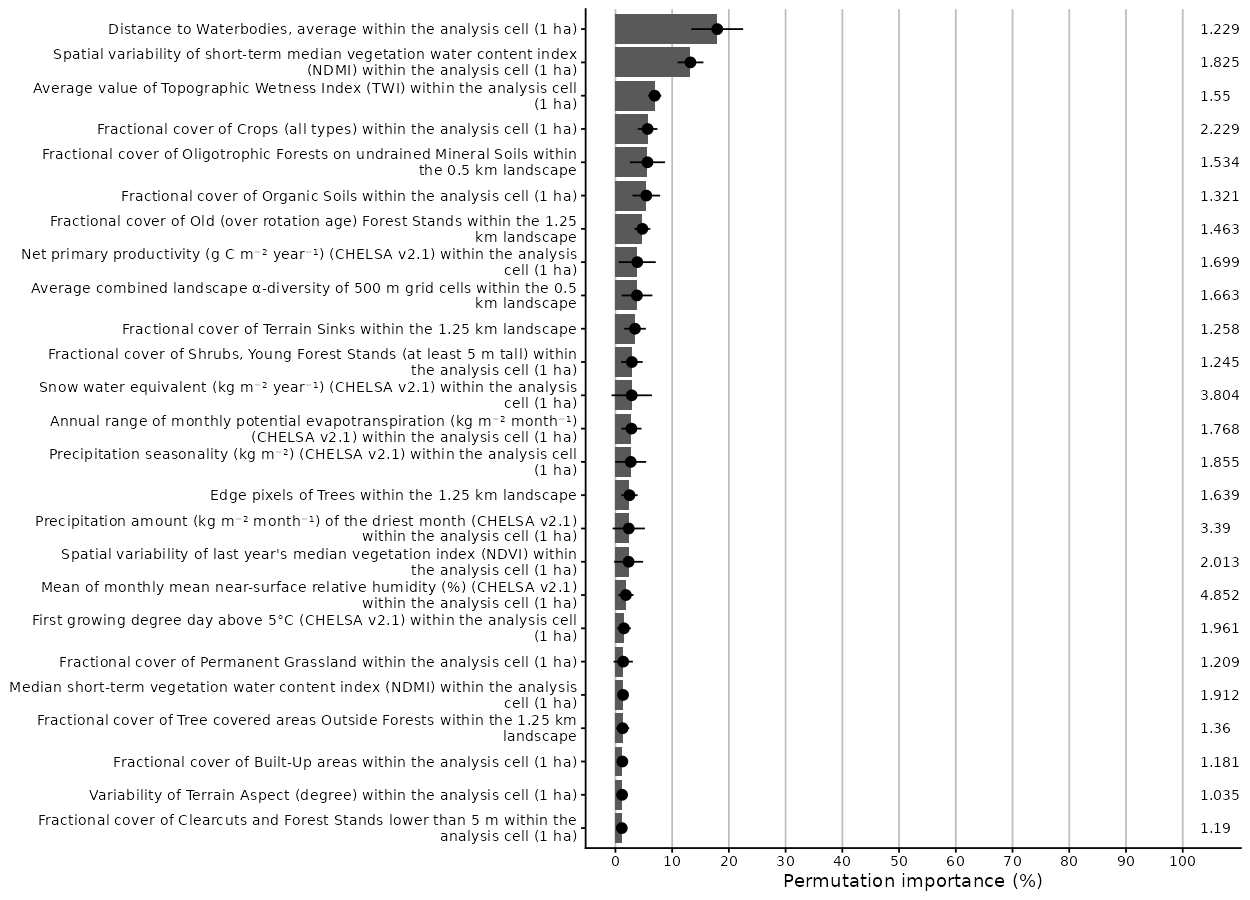
\includegraphics[width=1\linewidth,height=0.70\textheight,keepaspectratio]{results/NATNATv2b/PicVarImpVIFs_NATNAT.png}

\par\small\textit{Permutation-importance (mean and standard deviation from 99 permutations, on the x-axis) of the ecogeographical variables (first y-axis, left side), and their variance inflation factor values (second y-axis, right side). **For a full resolution refer to repository: link or online document: link**}\normalsize
\end{center}

\section*{Marginal responses}\label{marginal-responses-26}
\addcontentsline{toc}{section}{Marginal responses}

\begin{center}
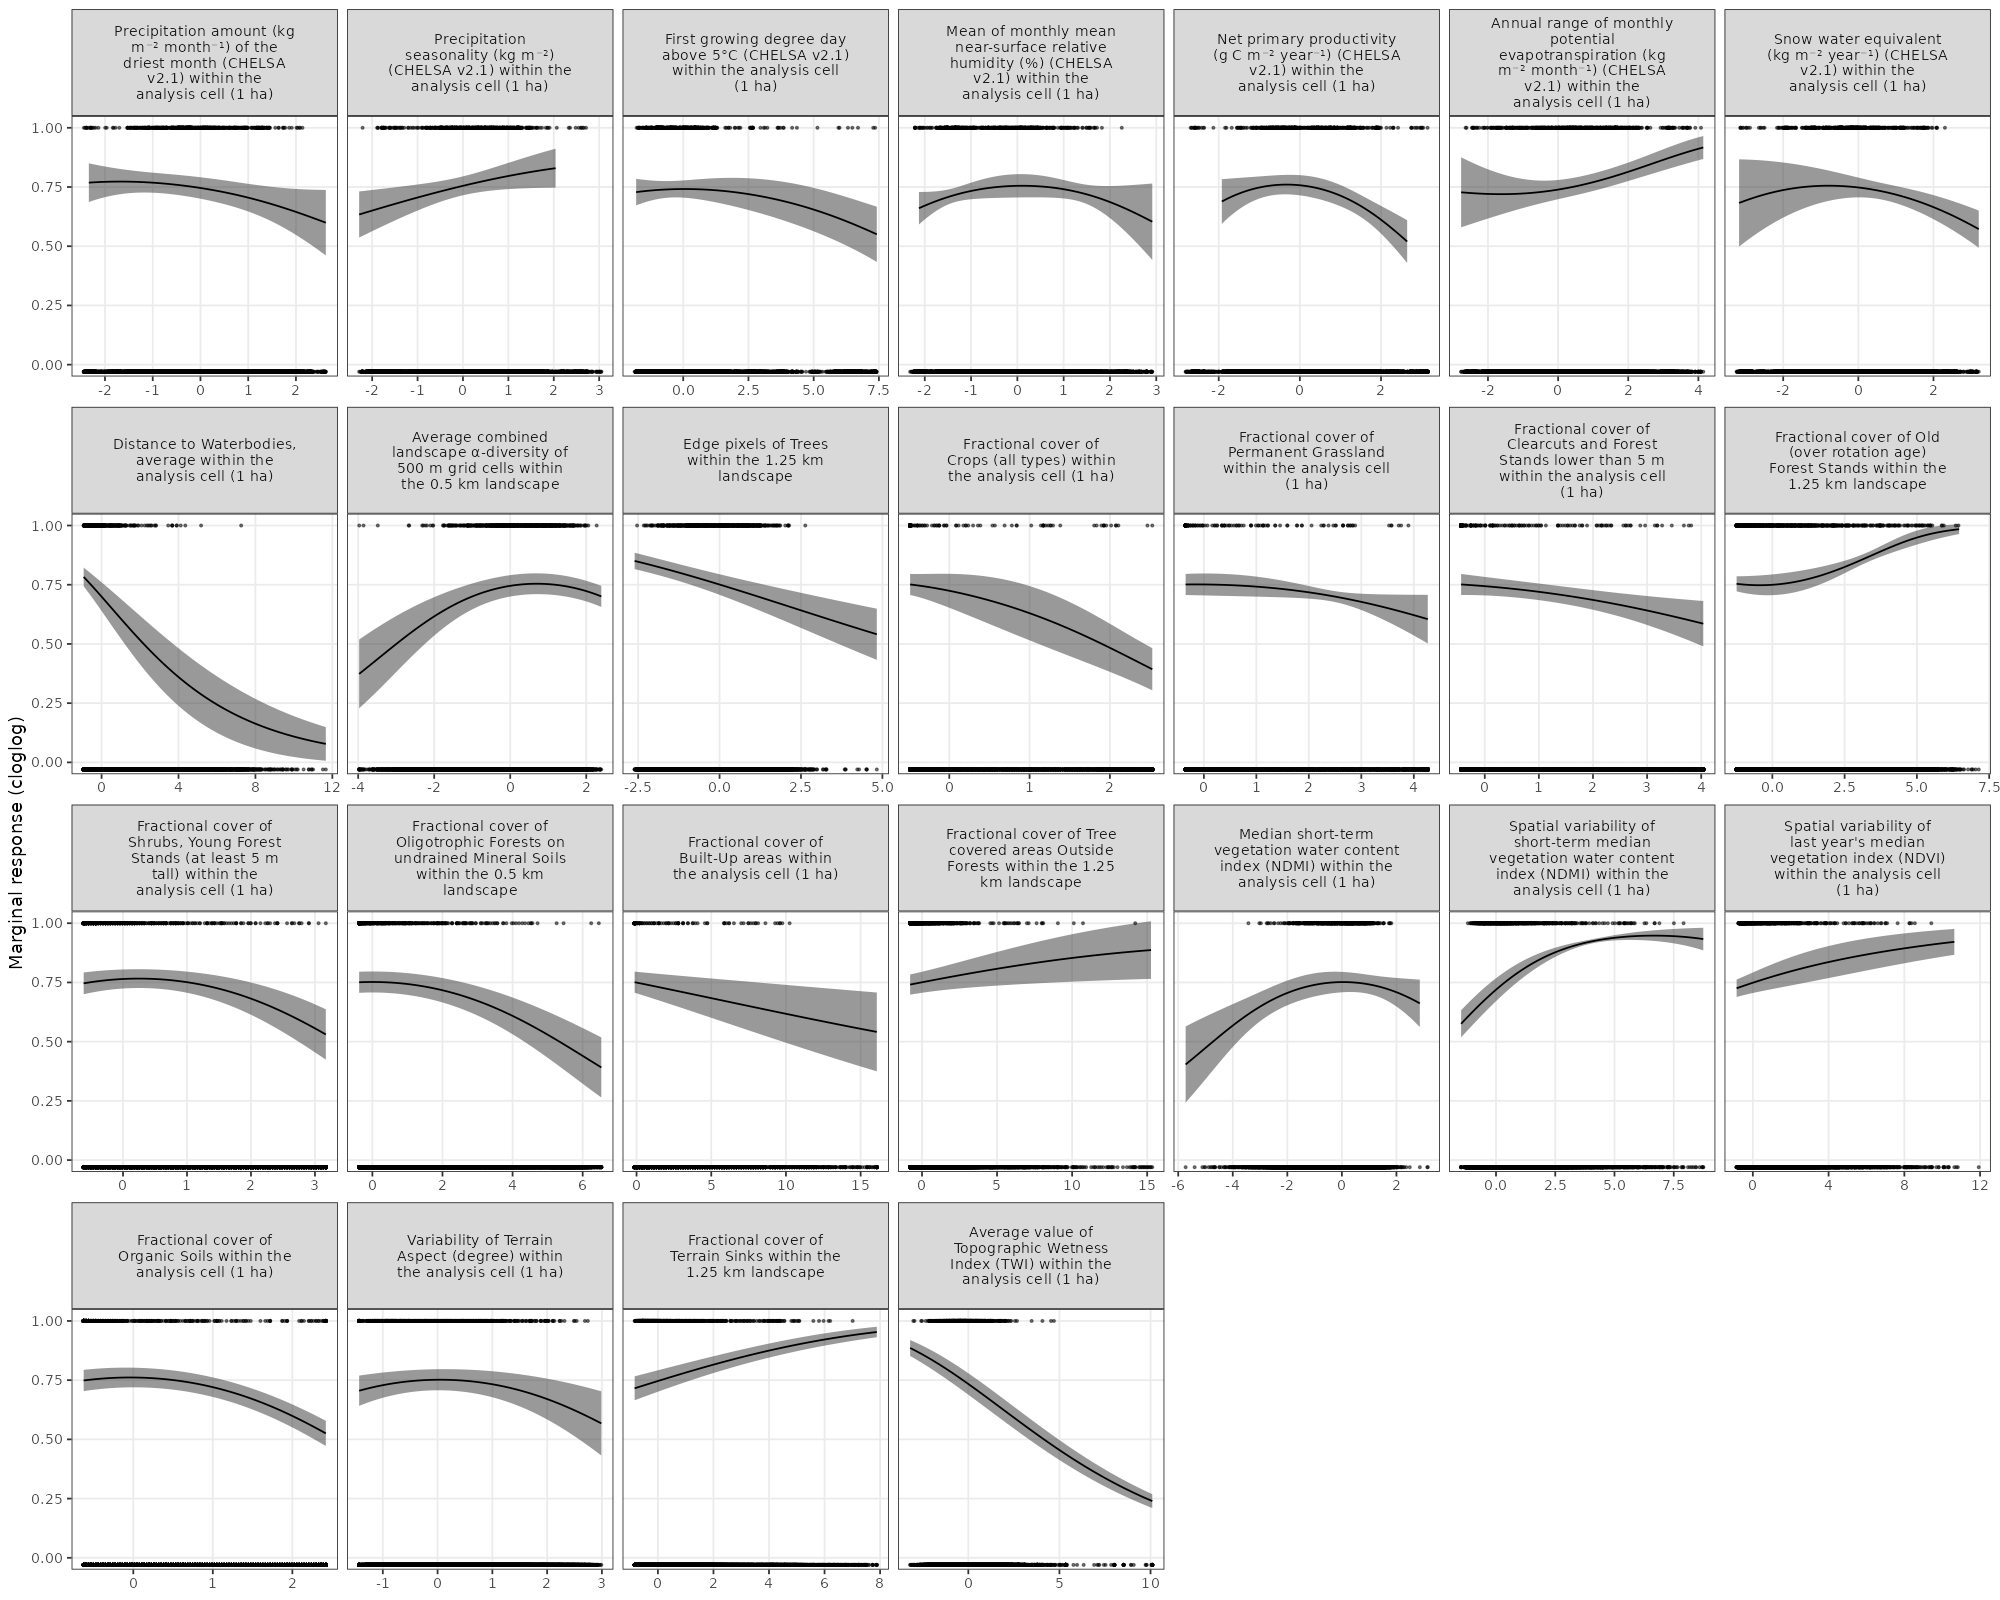
\includegraphics[width=1\linewidth,height=0.70\textheight,keepaspectratio]{results/NATNATv2b/PicMargResp_NATNAT.png}

\par\small\textit{Marginalised for arithmetic mean response curves illustrating the effect of each ecogeographical variable on the habitat suitability when all the other variables have their arithmetic mean values. The y-axis shows the predicted habitat suitability (cloglog-transformed), while the x-axis shows the standardised (centred and scaled) value of the ecogeographical variable. Dots at a value of 1 on the y-axis illustrate presence locations in the environment (on the x-axis), while dots at a value of 0 illustrate background locations used in modelling.  **For a full resolution refer to repository: link or online document: link**}\normalsize
\end{center}

\section*{Habitat and conservation associations}\label{habitat-and-conservation-associations-26}
\addcontentsline{toc}{section}{Habitat and conservation associations}

\begin{center}
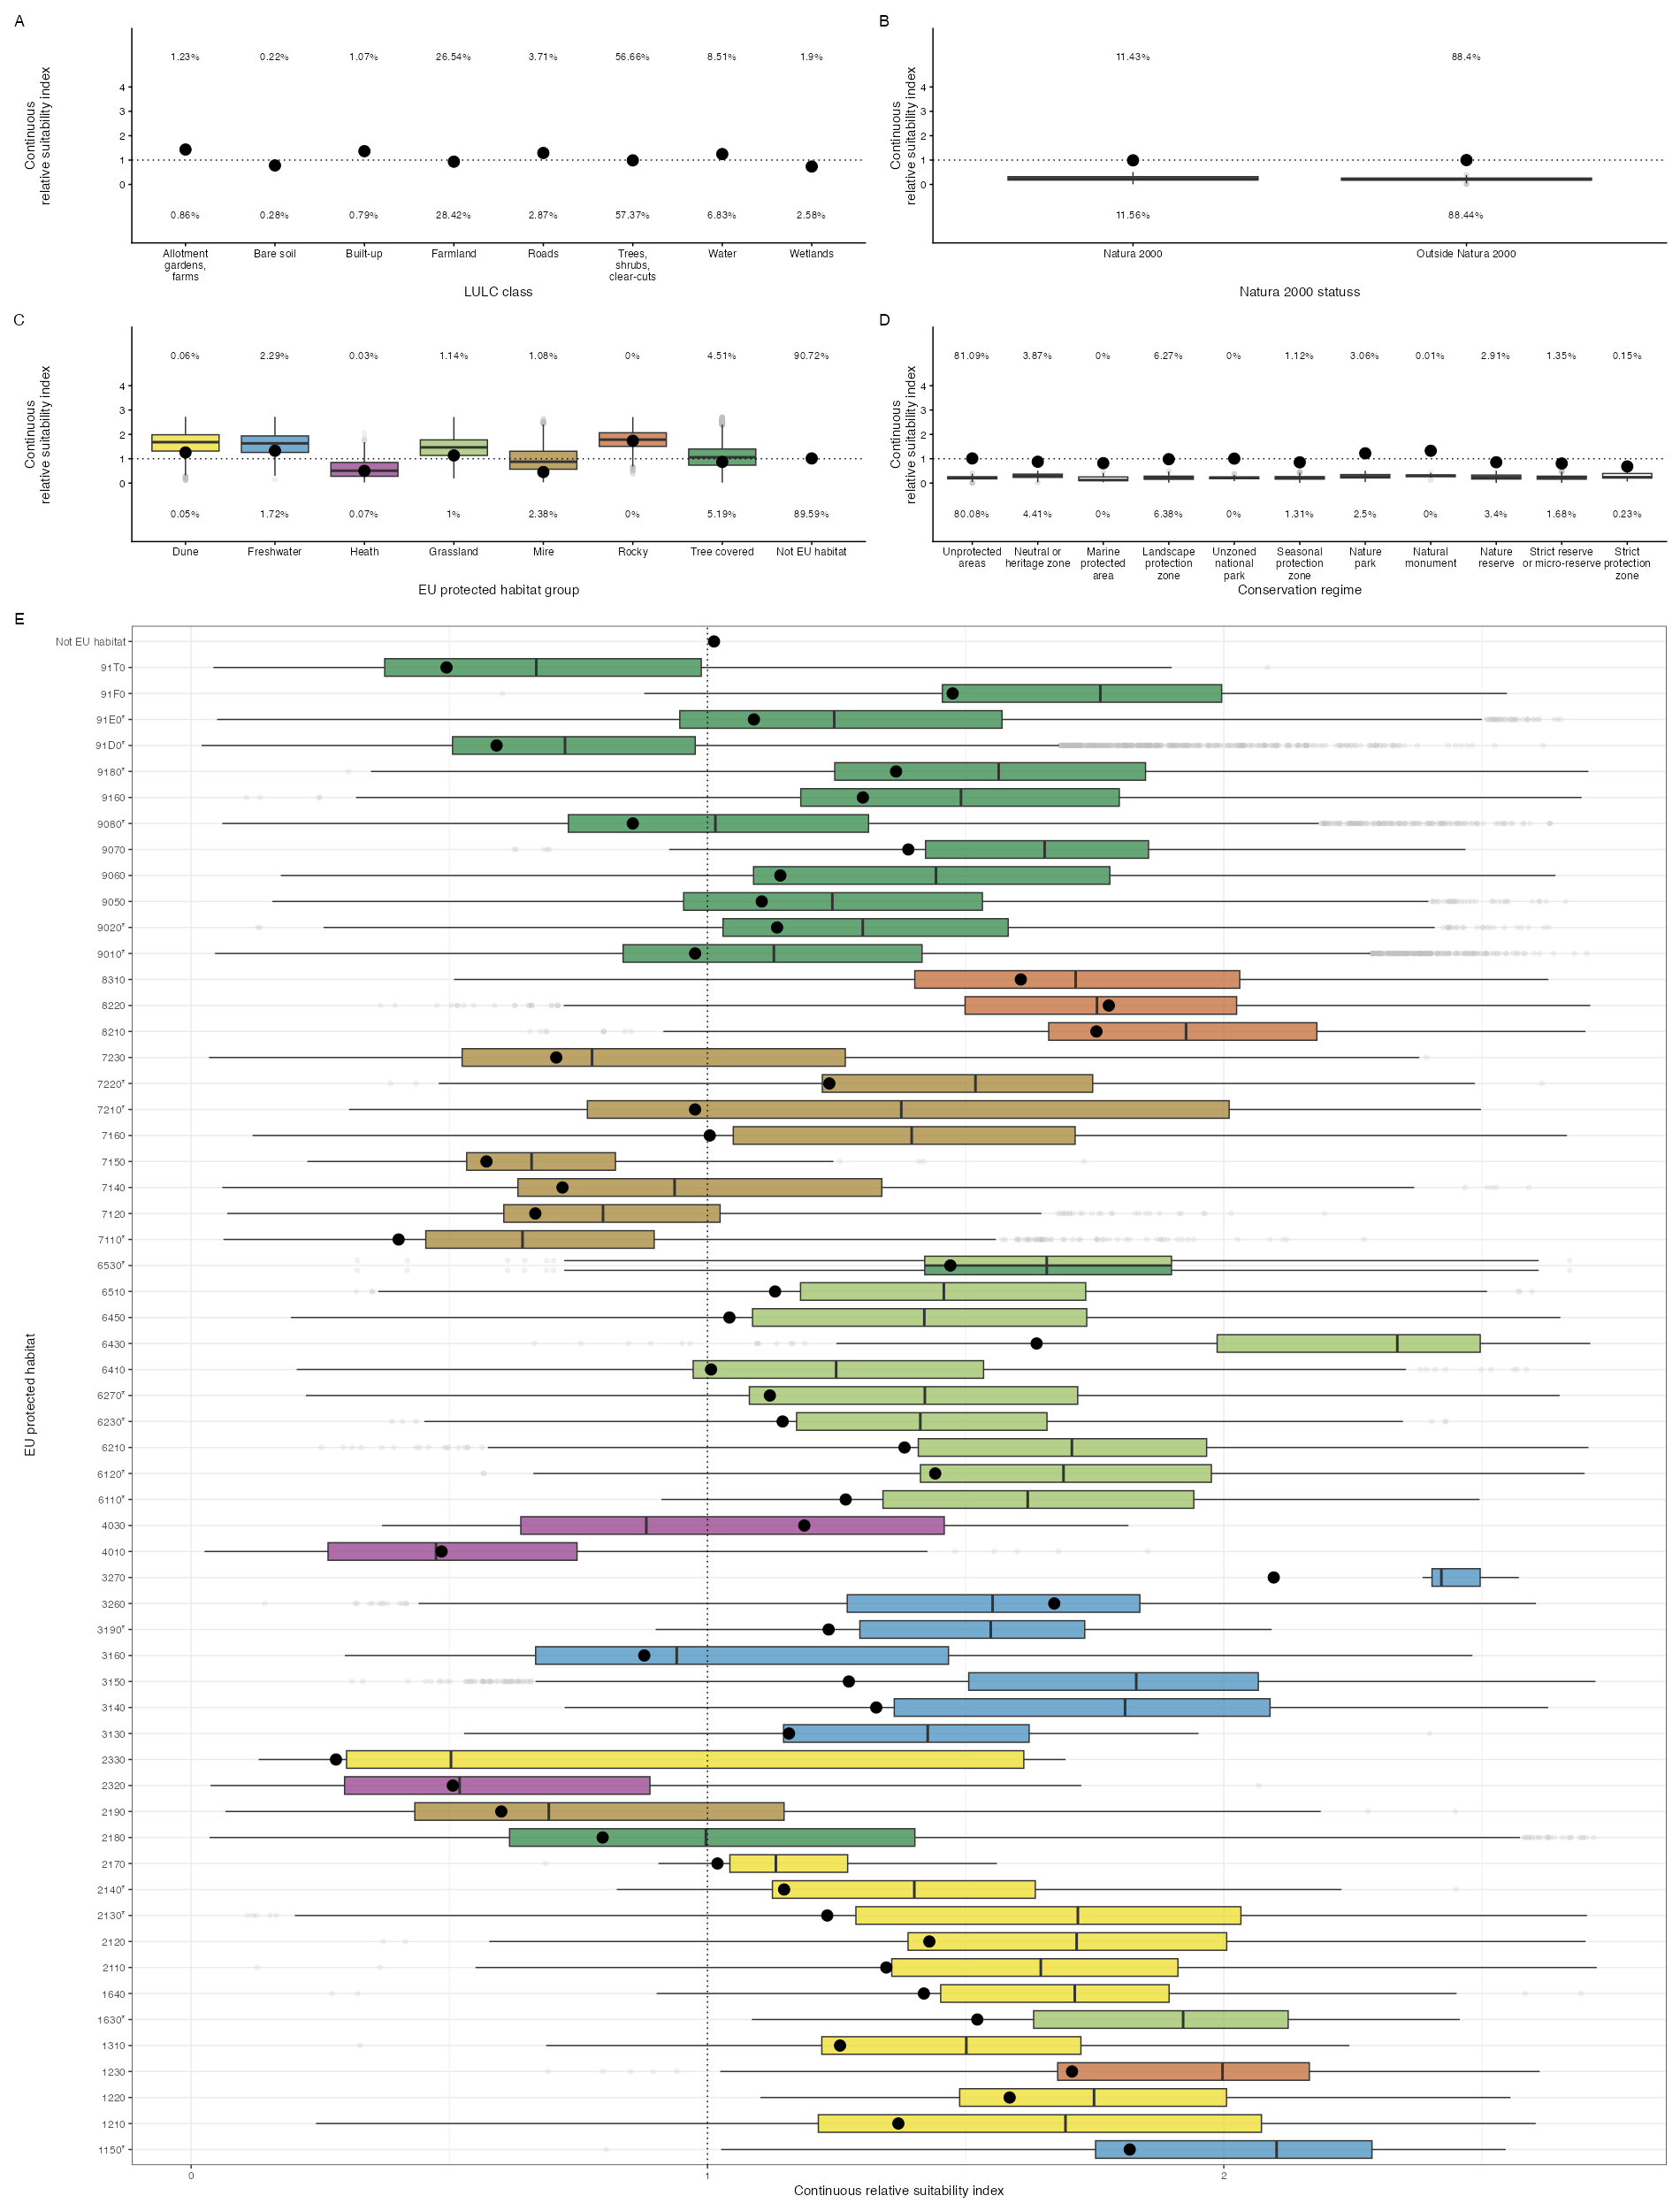
\includegraphics[width=1\linewidth,height=0.70\textheight,keepaspectratio]{results/NATNATv2b/PicAssoc_NATNAT.png}

\par\small\textit{Associations between predicted suitability and: (A) land use land cover classes, (B) Natura 2000 status, (C) stratified EU protected habitat classes, (D) conservation regime, and (E) EU protected habitats. The y-axis show continuous relative suitability index (derivative of Manly's index of preference). Colours in (C) and (E) correspond to stratified EU protected habitat classes. For classifications composed of multiple individual polygons, polygon-level indices were additionally calculated to show within-category variation. The figures therefore combine category-level estimates (points) with the distributions of polygon-level values (boxplots, where applicable). Labels above and below the panels report, respectively, the percentage of total predicted suitability and the percentage of mapped area represented by each category. **For a full resolution refer to repository: link or online document: link**}\normalsize
\end{center}

\section*{Conservation prioritization}\label{conservation-prioritization-26}
\addcontentsline{toc}{section}{Conservation prioritization}

\begin{center}
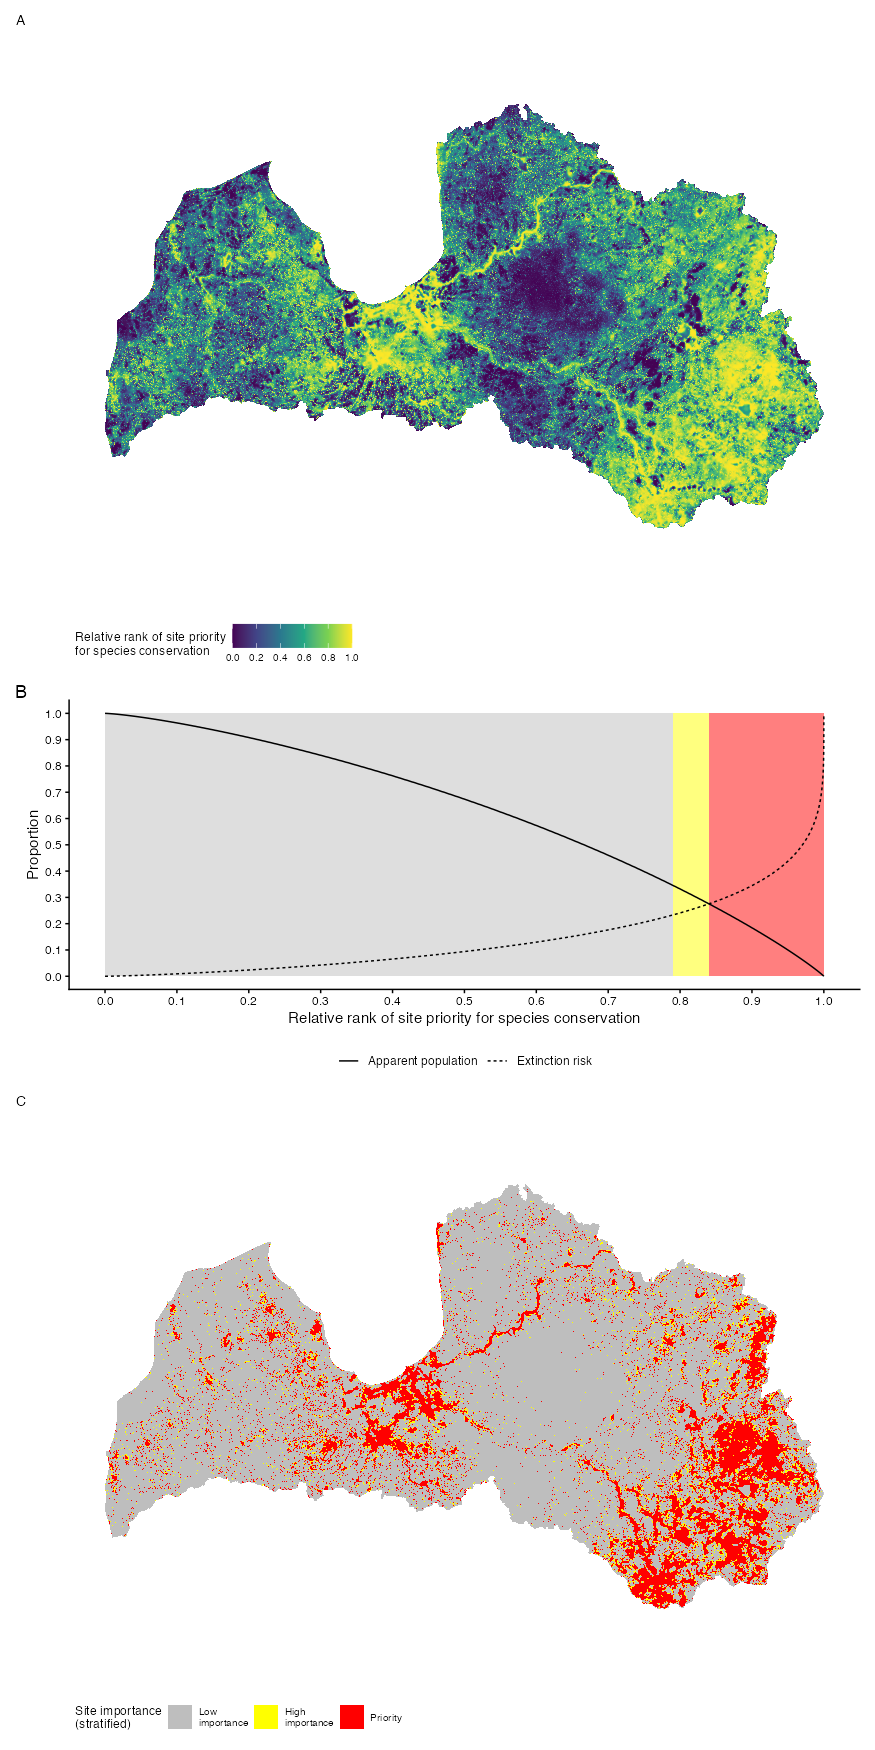
\includegraphics[width=0.85\linewidth,height=0.70\textheight,keepaspectratio]{results/NATNATv2b/PicPrior_NATNAT.png}

\par\small\textit{Single-species conservation prioritization focusing on maximisation of core area protection (CAZMAX) while accounting for site connectivity: (A) relative site rank; (B) relationship between apparent-population and extinction-risk curves with a simplified classification which is spatially demonstrated in the bootom row; (C) spatial distribution of proposed classification of site prioritization results. **For a full resolution refer to repository: link or online document: link**}\normalsize
\end{center}

\chapter*{\texorpdfstring{\emph{Vipera berus}}{Vipera berus}}\label{vipber}
\addcontentsline{toc}{chapter}{\emph{Vipera berus}}

\section*{Summary}\label{summary-27}
\addcontentsline{toc}{section}{Summary}

\subsection*{Model description}\label{model-description-27}
\addcontentsline{toc}{subsection}{Model description}

Occurrence and background data were divided into model-training with four block spatial cross-validation data and an independent test set. Sampling-bias/background treatment: \textbf{Phenology Weighted Target Group}. Observations were retained only where accumulated LULC change within the 1-ha analysis cell from the year of observation to 2024 did not exceed 50\%; observations were retained only where accumulated LULC change within the home-range radius around the analysis cell from the year of observation to 2024 did not exceed 50\%.

The final data set contained \textbf{187} presence records: \textbf{140} for training with four spatial block cross-validation and \textbf{47} for independent testing. Training background contained \textbf{29958} locations, with \textbf{10042} additional independent-test background locations.

\subsection*{Expert assessment scores}\label{expert-assessment-scores-27}
\addcontentsline{toc}{subsection}{Expert assessment scores}

\begin{itemize}
\tightlist
\item
  \textbf{Marginal responses and variable importance score:} 4 (good ecological interpretability)
\item
  \textbf{Map score:} 3 (moderate agreement with known distribution)
\item
  \textbf{Applicability score:} 3 (moderate applicability)
\end{itemize}

\textbf{Šo sadaļu aizpildām manuāli no ekspertu aptaujām}

\subsection*{Statistical evaluation}\label{statistical-evaluation-27}
\addcontentsline{toc}{subsection}{Statistical evaluation}

The final model had a training TSS of \textbf{0.401}, with a training-derived cloglog threshold of \textbf{0.539}. Combined training AUC was \textbf{0.772} and combined test AUC was \textbf{0.685}.

\subsubsection*{Spatial cross-validation}\label{spatial-cross-validation-27}
\addcontentsline{toc}{subsubsection}{Spatial cross-validation}

\begin{itemize}
\tightlist
\item
  \textbf{AUC:} 0.6967 ± 0.0214; null models: 0.508 ± 0.0226; z = 8.3455, p \textless{} 0.001
\item
  \textbf{CBI:} 0.8658 ± 0.1119; null models: 0 ± 0.1406; z = 6.1561, p \textless{} 0.001
\item
  \textbf{OR10:} 0.2286 ± 0.134; null models: 0.2314 ± 0.0765; z = -0.0374, p = 0.485
\item
  \textbf{ORmin:} 0.0214 ± 0.0274; null models: 0.0424 ± 0.0454; z = -0.4628, p = 0.322
\end{itemize}

\subsubsection*{Independent testing}\label{independent-testing-26}
\addcontentsline{toc}{subsubsection}{Independent testing}

\begin{itemize}
\tightlist
\item
  \textbf{TSS:} 0.256; \textbf{sensitivity:} 0.596; \textbf{specificity:} 0.66
\item
  \textbf{AUC:} 0.663; null models: 0.492 ± 0.0628; z = 2.7243, p = 0.003
\item
  \textbf{CBI:} 0.709; null models: -0.0613 ± 0.4446; z = 1.7325, p = 0.042
\item
  \textbf{OR10:} 0.277; null models: 0.1928 ± 0.0797; z = 1.0524, p = 0.854
\item
  \textbf{ORmin:} 0; null models: 0.0217 ± 0.0343; z = -0.6319, p = 0.264
\end{itemize}

\subsection*{Conservation prioritisation summary}\label{conservation-prioritisation-summary-27}
\addcontentsline{toc}{subsection}{Conservation prioritisation summary}

The primary priority area covers \textbf{15.3\%} of Latvia and contains \textbf{27.6\%} of the summed habitat suitability (apparent population proxy).

The broader high importance area covers \textbf{39.2\%} of Latvia and contains \textbf{58.6\%} of the summed habitat suitability.

For comparison, the area classified as suitable using the maximum training sensitivity plus specificity habitat-suitability threshold contains \textbf{58.6\%} of the summed continuous habitat suitability.

\subsection*{Version evolution}\label{version-evolution-27}
\addcontentsline{toc}{subsection}{Version evolution}

\textbf{Šo sadaļu aizpildām manuāli, izmntojot sagatavotās shēmas. Jāvienojas par to noformējumu}

\section*{Habitat suitability}\label{habitat-suitability-27}
\addcontentsline{toc}{section}{Habitat suitability}

\begin{center}
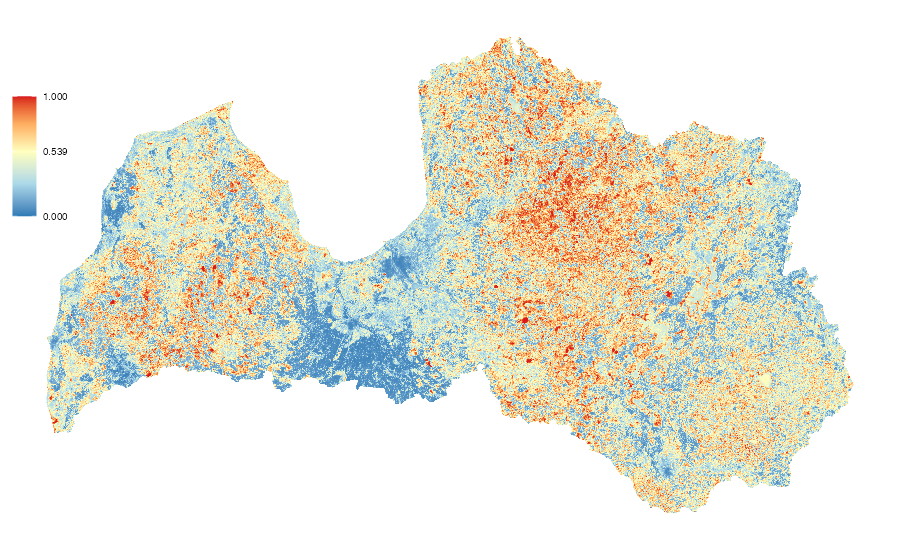
\includegraphics[width=1\linewidth,height=0.70\textheight,keepaspectratio]{results/VIPBERv2a5/PicHSmap_VIPBER.png}

\par\small\textit{Predicted continuous habitat suitability across Latvia. The warmer the colour the higher is the predicted habitat suitability. Value in the middle of the legend correspond to the maximum training sensitivity plus specificity threshold. **For a full resolution refer to repository: link or online document: link**}\normalsize
\end{center}

\section*{Model thresholds}\label{model-thresholds-27}
\addcontentsline{toc}{section}{Model thresholds}

Threshold values and associated omission rates

\begin{center}
\resizebox{\linewidth}{!}{%

\begin{tabular}{lrrrrr}
\toprule
Threshold & Cloglog value & Fractional predicted area & Training omission rate & Test omission rate & P-values\\
\midrule
Minimum training presence & 0.1976458 & 0.8893702 & 0.0000000 & 0.0000000 & 0\\
Equal training sensitivity and specificity & 0.5781158 & 0.3087304 & 0.3071429 & 0.0022748 & 0\\
Maximum training sensitivity plus specificity & 0.5391913 & 0.3646451 & 0.1928571 & 0.0018791 & 0\\
Equal test sensitivity and specificity & 0.5059618 & 0.4155282 & 0.1642857 & 0.0017802 & 0\\
Maximum test sensitivity plus specificity & 0.3970760 & 0.5853049 & 0.0857143 & 0.0005934 & 0\\
\bottomrule
\end{tabular}
}
\end{center}

\section*{Variable importance}\label{variable-importance-27}
\addcontentsline{toc}{section}{Variable importance}

\begin{center}
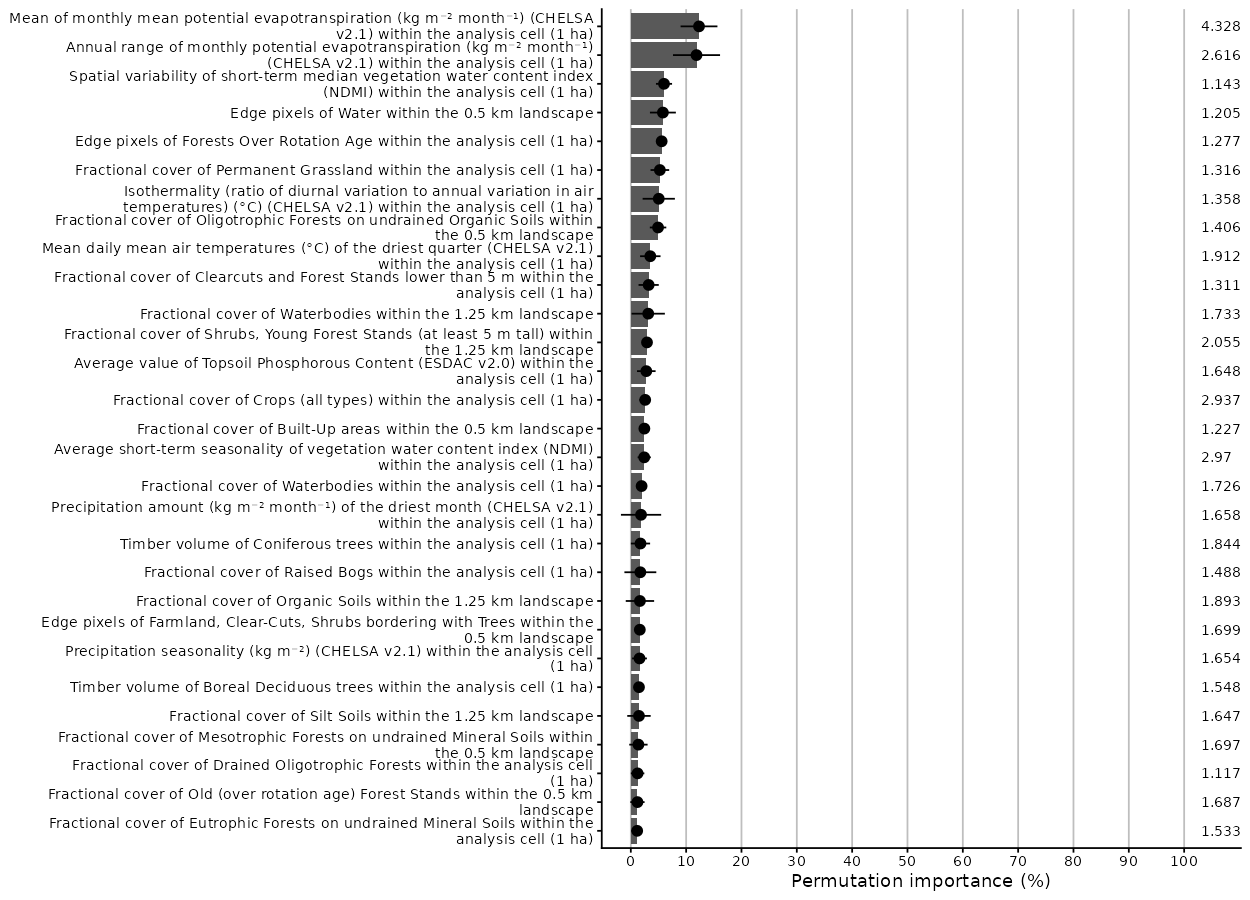
\includegraphics[width=1\linewidth,height=0.70\textheight,keepaspectratio]{results/VIPBERv2a5/PicVarImpVIFs_VIPBER.png}

\par\small\textit{Permutation-importance (mean and standard deviation from 99 permutations, on the x-axis) of the ecogeographical variables (first y-axis, left side), and their variance inflation factor values (second y-axis, right side). **For a full resolution refer to repository: link or online document: link**}\normalsize
\end{center}

\section*{Marginal responses}\label{marginal-responses-27}
\addcontentsline{toc}{section}{Marginal responses}

\begin{center}
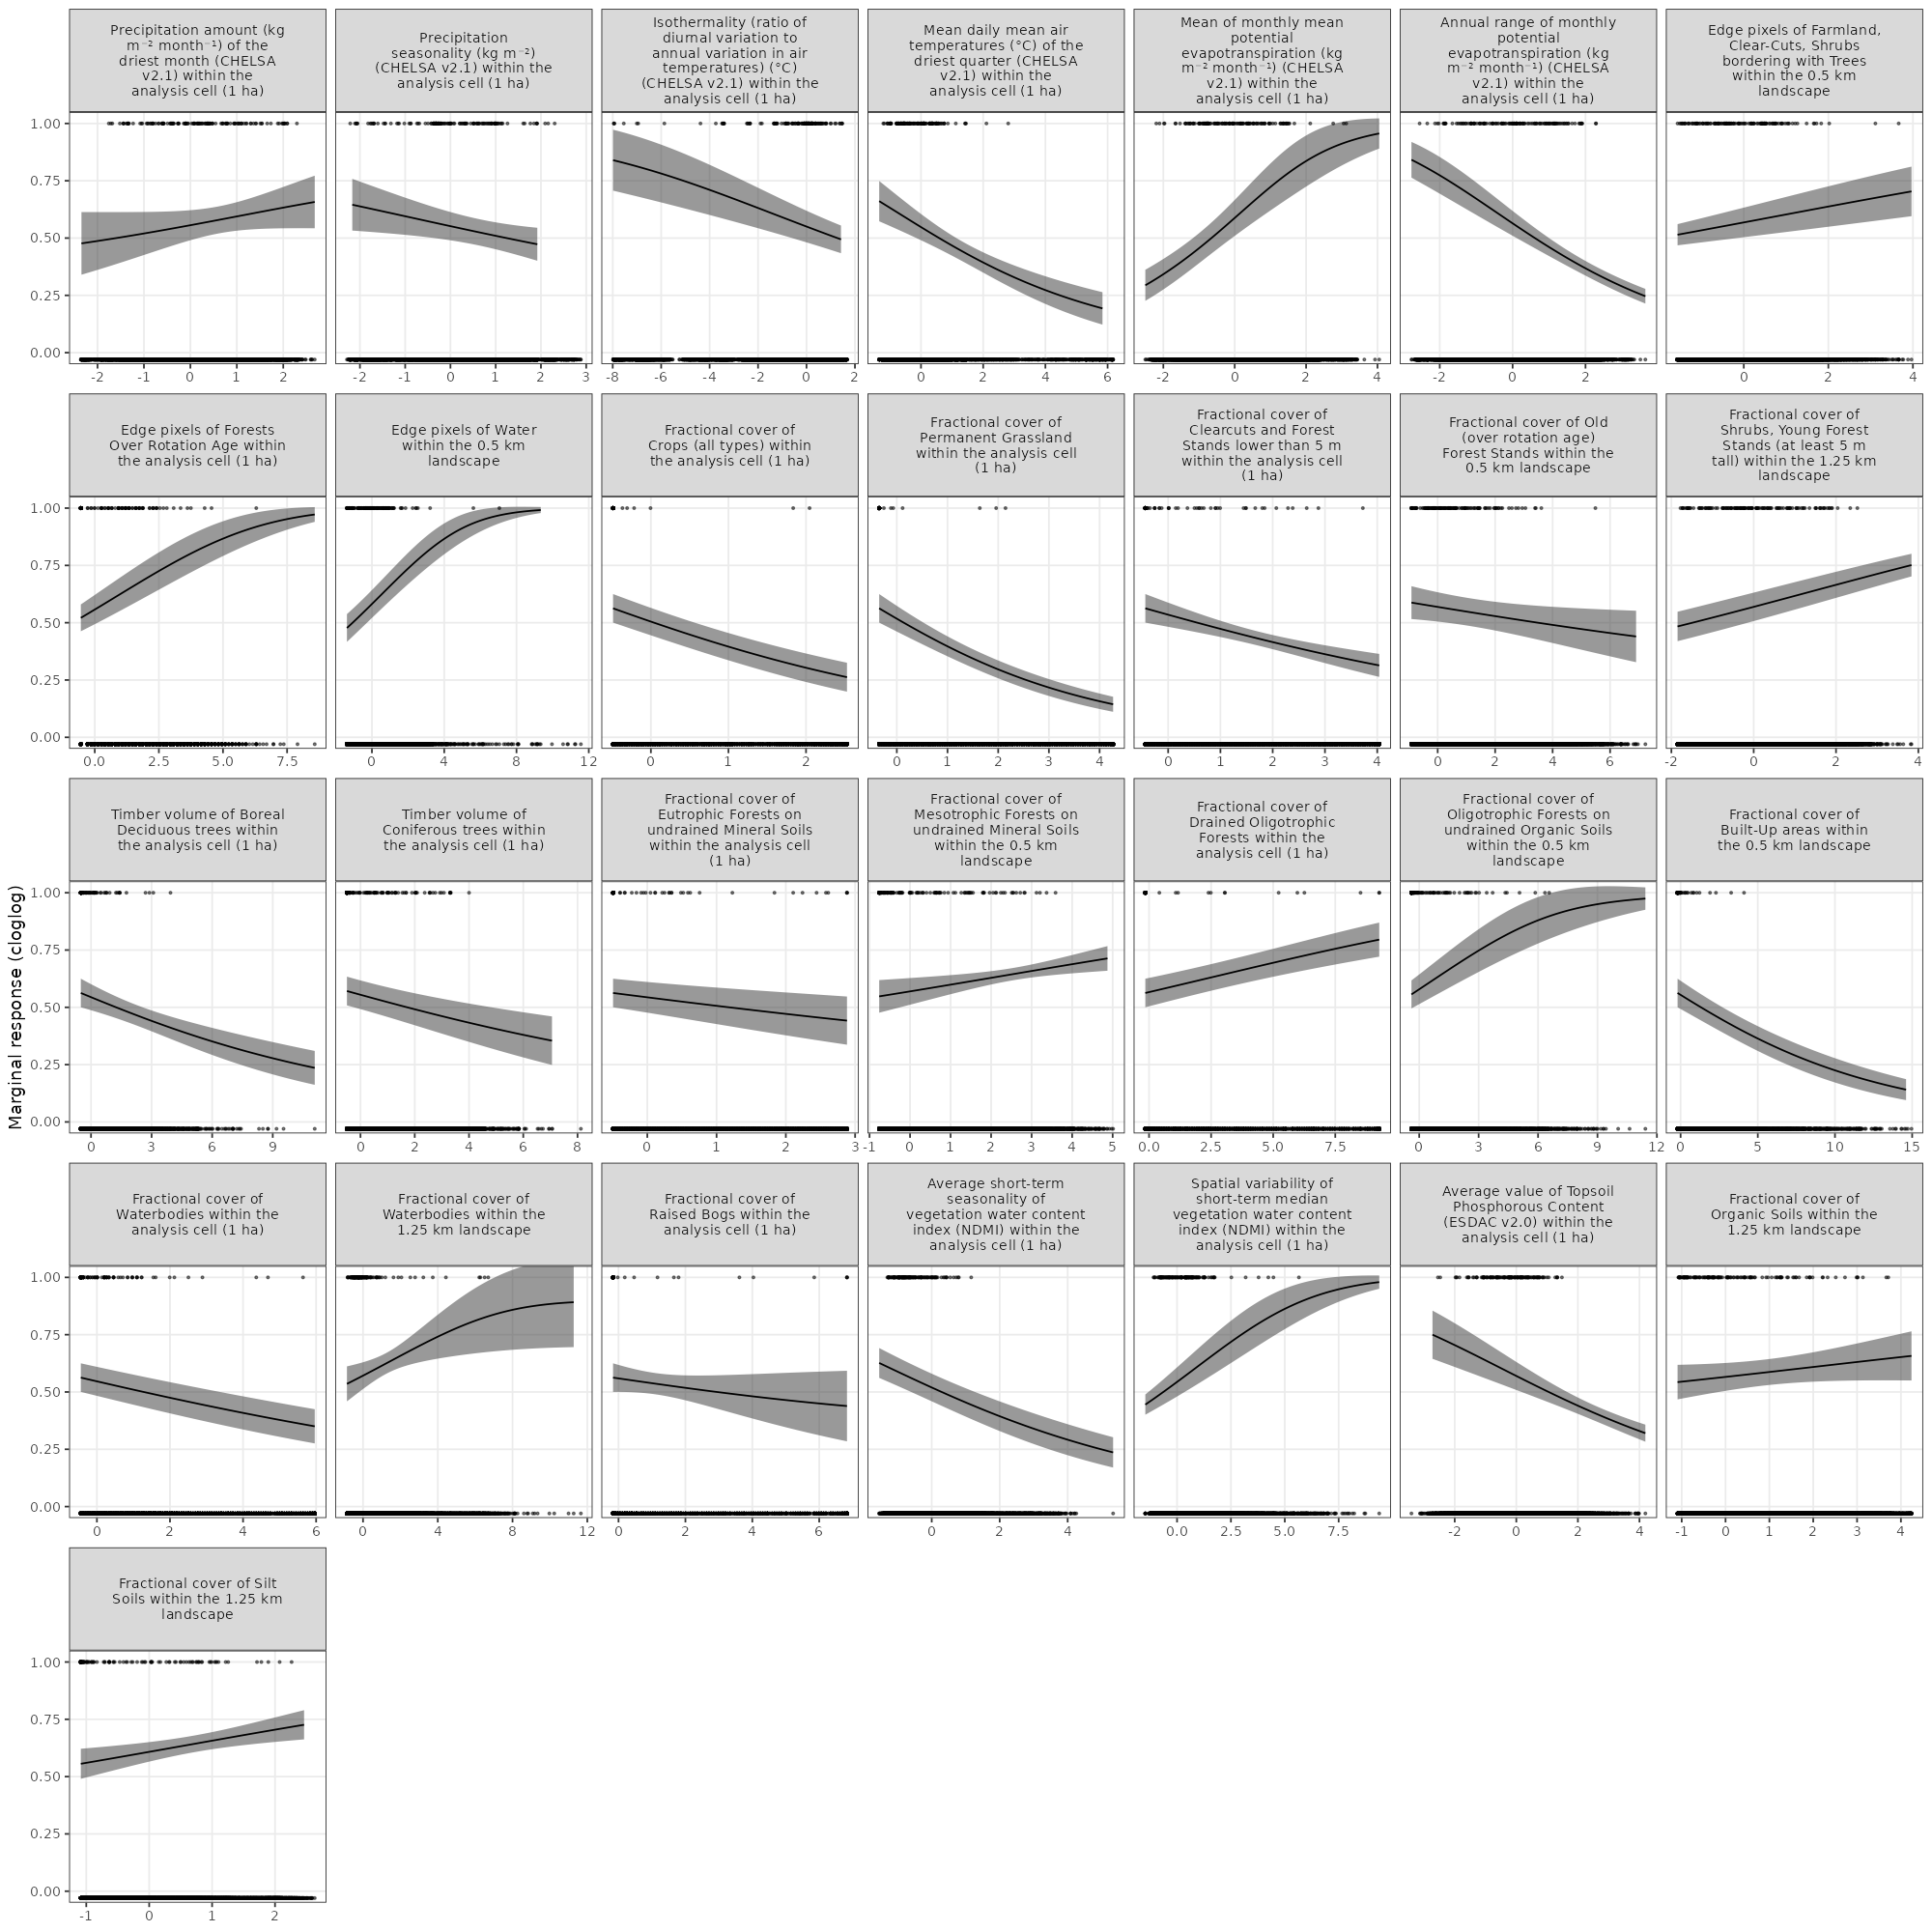
\includegraphics[width=1\linewidth,height=0.70\textheight,keepaspectratio]{results/VIPBERv2a5/PicMargResp_VIPBER.png}

\par\small\textit{Marginalised for arithmetic mean response curves illustrating the effect of each ecogeographical variable on the habitat suitability when all the other variables have their arithmetic mean values. The y-axis shows the predicted habitat suitability (cloglog-transformed), while the x-axis shows the standardised (centred and scaled) value of the ecogeographical variable. Dots at a value of 1 on the y-axis illustrate presence locations in the environment (on the x-axis), while dots at a value of 0 illustrate background locations used in modelling.  **For a full resolution refer to repository: link or online document: link**}\normalsize
\end{center}

\section*{Habitat and conservation associations}\label{habitat-and-conservation-associations-27}
\addcontentsline{toc}{section}{Habitat and conservation associations}

\begin{center}
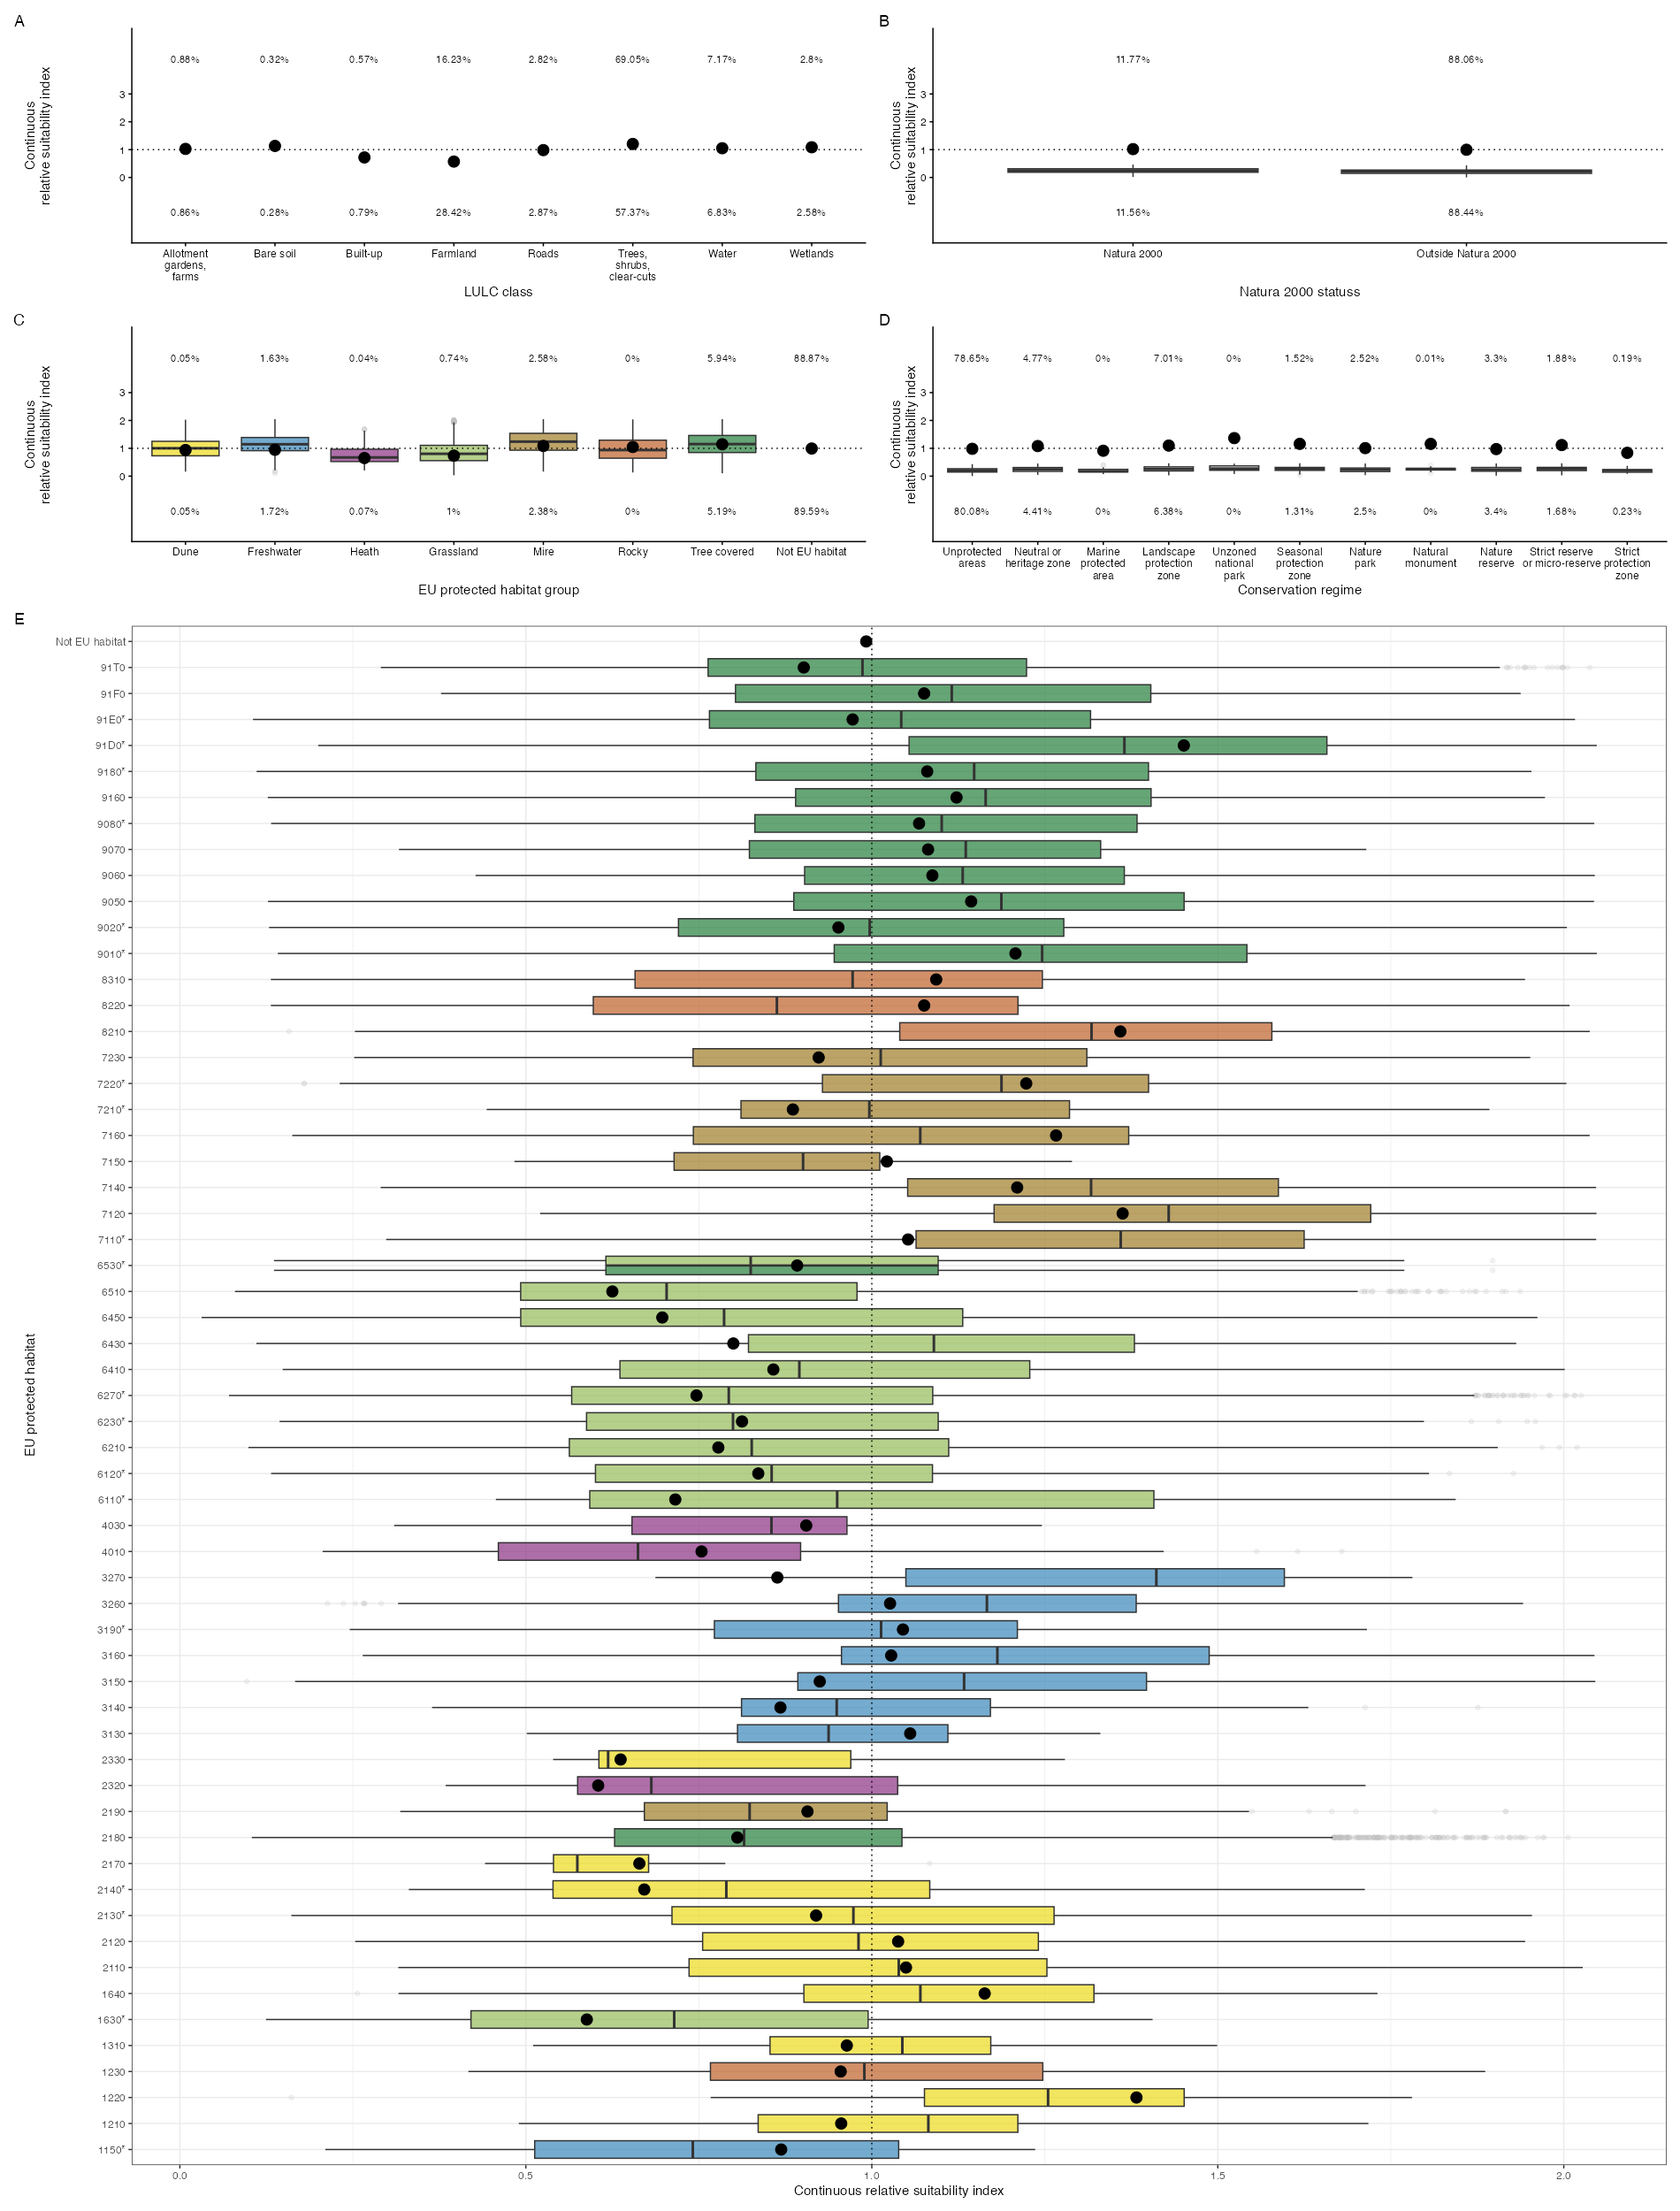
\includegraphics[width=1\linewidth,height=0.70\textheight,keepaspectratio]{results/VIPBERv2a5/PicAssoc_VIPBER.png}

\par\small\textit{Associations between predicted suitability and: (A) land use land cover classes, (B) Natura 2000 status, (C) stratified EU protected habitat classes, (D) conservation regime, and (E) EU protected habitats. The y-axis show continuous relative suitability index (derivative of Manly's index of preference). Colours in (C) and (E) correspond to stratified EU protected habitat classes. For classifications composed of multiple individual polygons, polygon-level indices were additionally calculated to show within-category variation. The figures therefore combine category-level estimates (points) with the distributions of polygon-level values (boxplots, where applicable). Labels above and below the panels report, respectively, the percentage of total predicted suitability and the percentage of mapped area represented by each category. **For a full resolution refer to repository: link or online document: link**}\normalsize
\end{center}

\section*{Conservation prioritization}\label{conservation-prioritization-27}
\addcontentsline{toc}{section}{Conservation prioritization}

\begin{center}
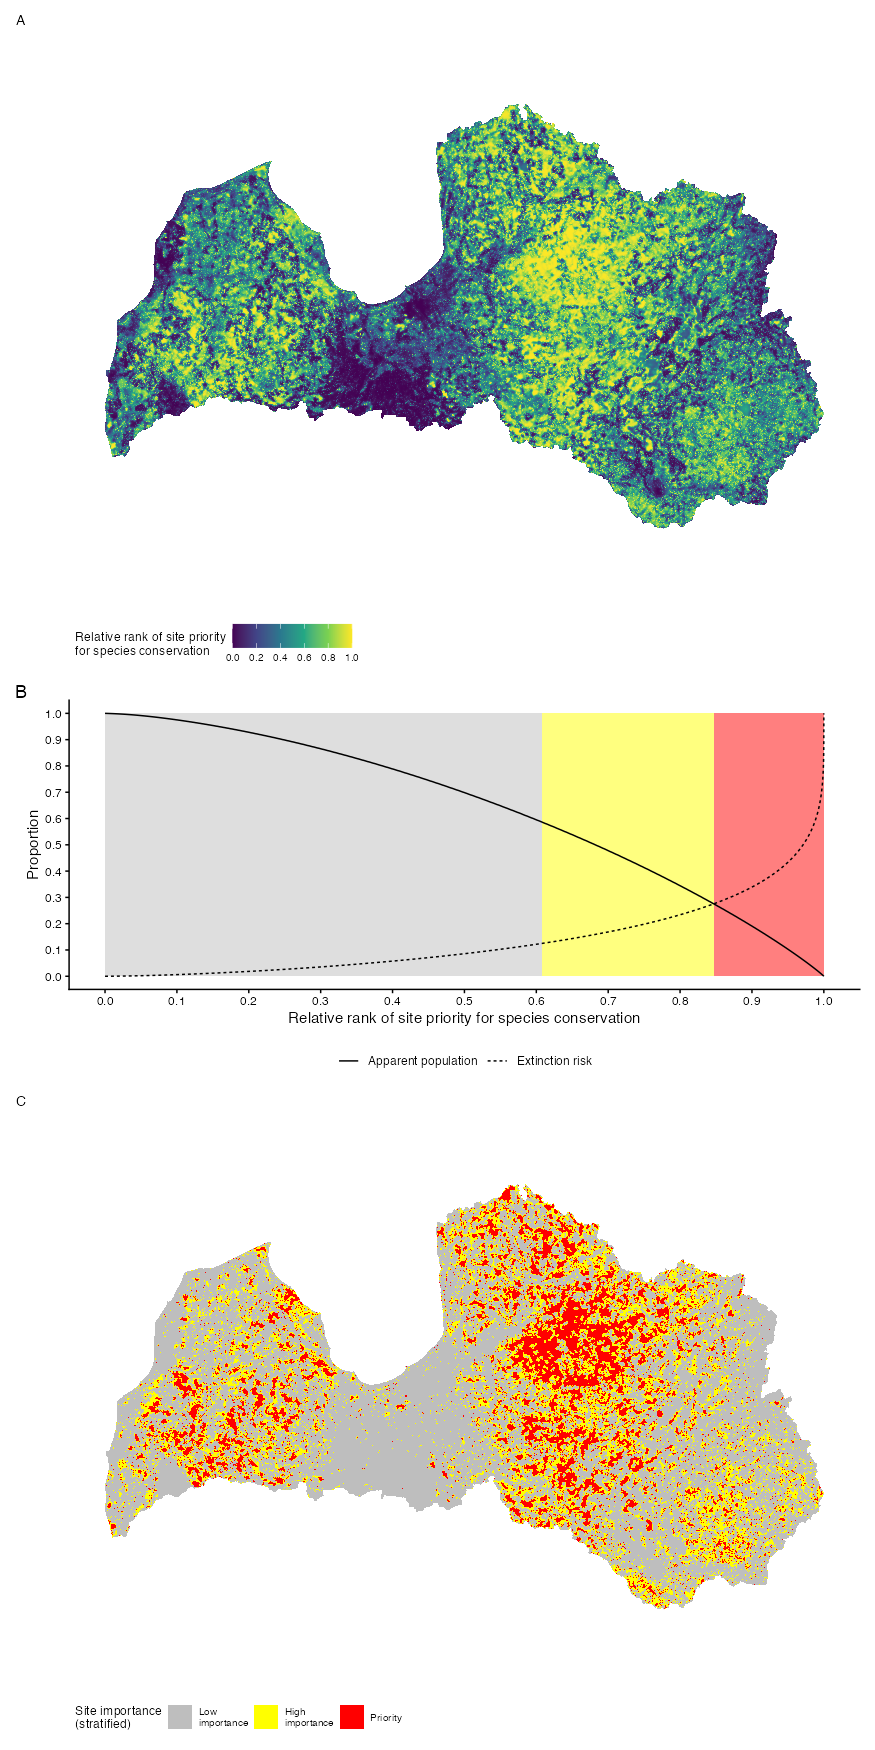
\includegraphics[width=0.85\linewidth,height=0.70\textheight,keepaspectratio]{results/VIPBERv2a5/PicPrior_VIPBER.png}

\par\small\textit{Single-species conservation prioritization focusing on maximisation of core area protection (CAZMAX) while accounting for site connectivity: (A) relative site rank; (B) relationship between apparent-population and extinction-risk curves with a simplified classification which is spatially demonstrated in the bootom row; (C) spatial distribution of proposed classification of site prioritization results. **For a full resolution refer to repository: link or online document: link**}\normalsize
\end{center}

\chapter*{\texorpdfstring{\emph{Anguis sp.}}{Anguis sp.}}\label{angspp}
\addcontentsline{toc}{chapter}{\emph{Anguis sp.}}

\section*{Summary}\label{summary-28}
\addcontentsline{toc}{section}{Summary}

\subsection*{Model description}\label{model-description-28}
\addcontentsline{toc}{subsection}{Model description}

Occurrence and background data were divided into model-training with four block spatial cross-validation data and an independent test set. Sampling-bias/background treatment: \textbf{Phenology Weighted Target Group}. Accumulated LULC change within the 1-ha analysis cell was not evaluated; accumulated LULC change within the home-range radius around the analysis cell was not evaluated.

The final data set contained \textbf{562} presence records: \textbf{422} for training with four spatial block cross-validation and \textbf{140} for independent testing. Training background contained \textbf{30013} locations, with \textbf{9987} additional independent-test background locations.

\subsection*{Expert assessment scores}\label{expert-assessment-scores-28}
\addcontentsline{toc}{subsection}{Expert assessment scores}

\begin{itemize}
\tightlist
\item
  \textbf{Marginal responses and variable importance score:} 4 (good ecological interpretability)
\item
  \textbf{Map score:} 4 (good agreement with known distribution)
\item
  \textbf{Applicability score:} 4 (high applicability)
\end{itemize}

\textbf{Šo sadaļu aizpildām manuāli no ekspertu aptaujām}

\subsection*{Statistical evaluation}\label{statistical-evaluation-28}
\addcontentsline{toc}{subsection}{Statistical evaluation}

The final model had a training TSS of \textbf{0.401}, with a training-derived cloglog threshold of \textbf{0.437}. Combined training AUC was \textbf{0.765} and combined test AUC was \textbf{0.764}.

\subsubsection*{Spatial cross-validation}\label{spatial-cross-validation-28}
\addcontentsline{toc}{subsubsection}{Spatial cross-validation}

\begin{itemize}
\tightlist
\item
  \textbf{AUC:} 0.7017 ± 0.0507; null models: 0.522 ± 0.0187; z = 9.6249, p \textless{} 0.001
\item
  \textbf{CBI:} 0.9152 ± 0.0403; null models: 0.1818 ± 0.1441; z = 5.0879, p \textless{} 0.001
\item
  \textbf{OR10:} 0.1601 ± 0.0949; null models: 0.1351 ± 0.059; z = 0.4239, p = 0.664
\item
  \textbf{ORmin:} 0.0096 ± 0.0192; null models: 0.0067 ± 0.0123; z = 0.2383, p = 0.594
\end{itemize}

\subsubsection*{Independent testing}\label{independent-testing-27}
\addcontentsline{toc}{subsubsection}{Independent testing}

\begin{itemize}
\tightlist
\item
  \textbf{TSS:} 0.389; \textbf{sensitivity:} 0.836; \textbf{specificity:} 0.553
\item
  \textbf{AUC:} 0.748; null models: 0.5173 ± 0.0774; z = 2.9801, p = 0.001
\item
  \textbf{CBI:} 0.861; null models: 0.0896 ± 0.5176; z = 1.4904, p = 0.068
\item
  \textbf{OR10:} 0.1; null models: 0.1168 ± 0.0725; z = -0.2317, p = 0.408
\item
  \textbf{ORmin:} 0; null models: 0.0031 ± 0.0111; z = -0.2834, p = 0.388
\end{itemize}

\subsection*{Conservation prioritisation summary}\label{conservation-prioritisation-summary-28}
\addcontentsline{toc}{subsection}{Conservation prioritisation summary}

The primary priority area covers \textbf{9.2\%} of Latvia and contains \textbf{27.5\%} of the summed habitat suitability (apparent population proxy).

The broader high importance area covers \textbf{19.8\%} of Latvia and contains \textbf{48.5\%} of the summed habitat suitability.

For comparison, the area classified as suitable using the maximum training sensitivity plus specificity habitat-suitability threshold contains \textbf{48.5\%} of the summed continuous habitat suitability.

\subsection*{Version evolution}\label{version-evolution-28}
\addcontentsline{toc}{subsection}{Version evolution}

\textbf{Šo sadaļu aizpildām manuāli, izmntojot sagatavotās shēmas. Jāvienojas par to noformējumu}

\section*{Habitat suitability}\label{habitat-suitability-28}
\addcontentsline{toc}{section}{Habitat suitability}

\begin{center}
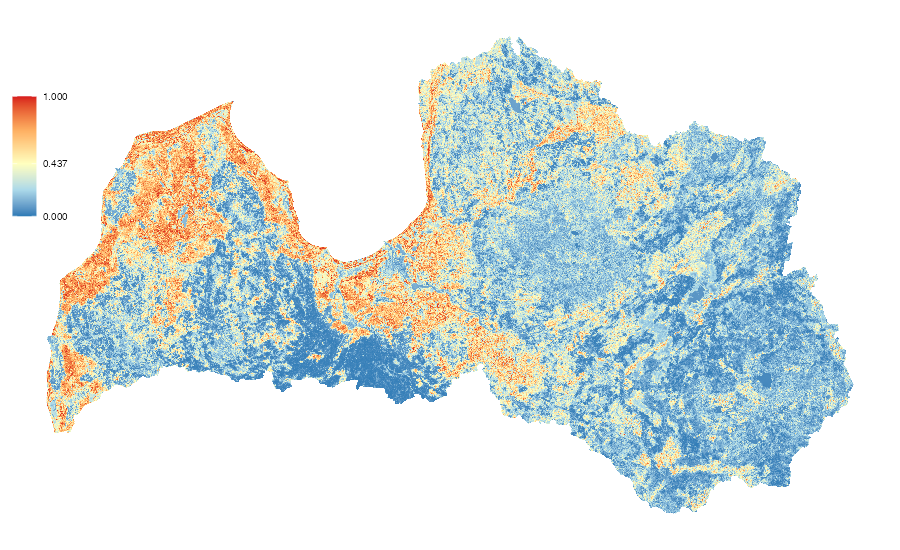
\includegraphics[width=1\linewidth,height=0.70\textheight,keepaspectratio]{results/ANGSPPv2b/PicHSmap_ANGSPP.png}

\par\small\textit{Predicted continuous habitat suitability across Latvia. The warmer the colour the higher is the predicted habitat suitability. Value in the middle of the legend correspond to the maximum training sensitivity plus specificity threshold. **For a full resolution refer to repository: link or online document: link**}\normalsize
\end{center}

\section*{Model thresholds}\label{model-thresholds-28}
\addcontentsline{toc}{section}{Model thresholds}

Threshold values and associated omission rates

\begin{center}
\resizebox{\linewidth}{!}{%

\begin{tabular}{lrrrrr}
\toprule
Threshold & Cloglog value & Fractional predicted area & Training omission rate & Test omission rate & P-values\\
\midrule
Minimum training presence & 0.1149647 & 0.9136712 & 0.0000000 & 0.0000000 & 0\\
Equal training sensitivity and specificity & 0.5663141 & 0.3104269 & 0.3104265 & 0.0044170 & 0\\
Maximum training sensitivity plus specificity & 0.4374440 & 0.4635919 & 0.1350711 & 0.0022576 & 0\\
Equal test sensitivity and specificity & 0.5529535 & 0.3250297 & 0.2962085 & 0.0042207 & 0\\
Maximum test sensitivity plus specificity & 0.6206677 & 0.2508590 & 0.3815166 & 0.0048096 & 0\\
\bottomrule
\end{tabular}
}
\end{center}

\section*{Variable importance}\label{variable-importance-28}
\addcontentsline{toc}{section}{Variable importance}

\begin{center}
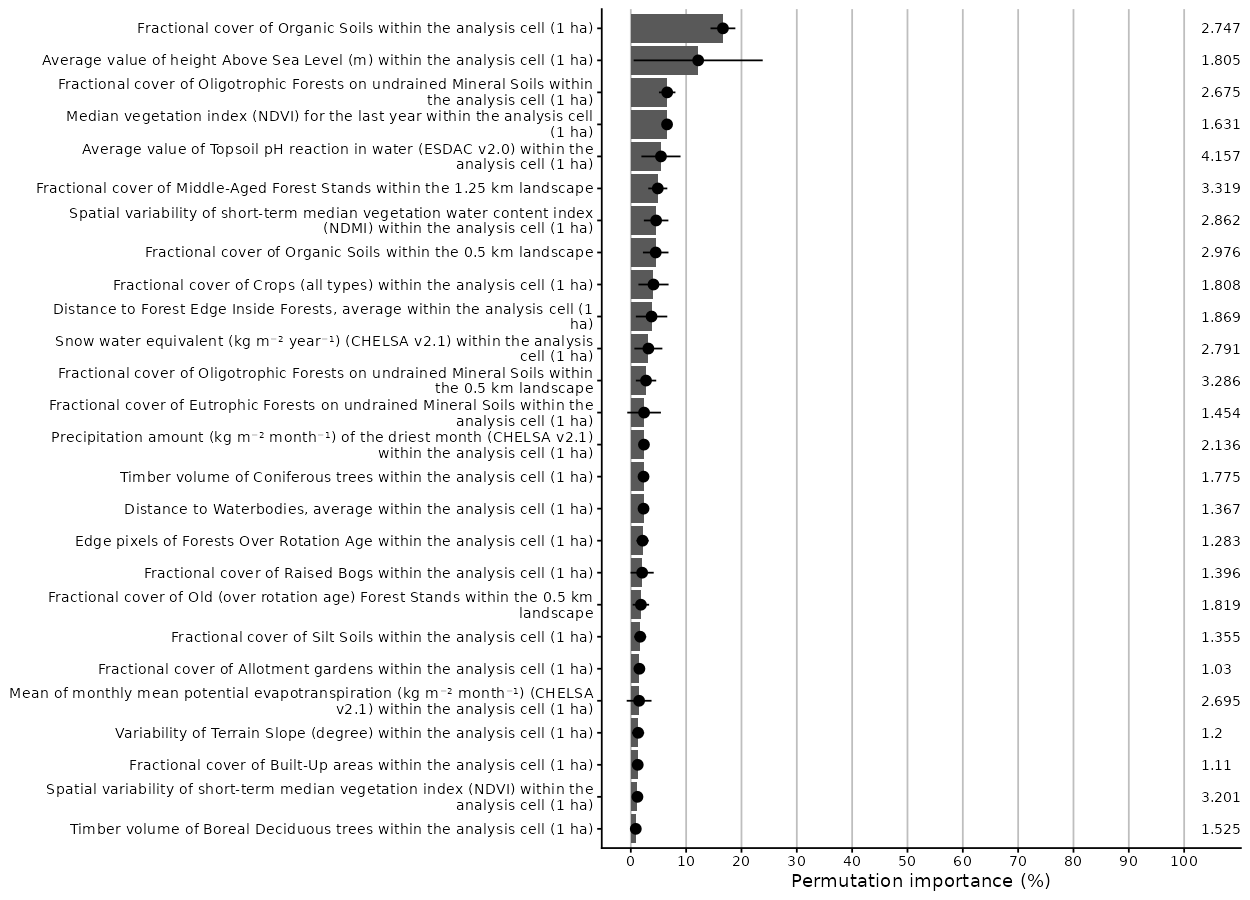
\includegraphics[width=1\linewidth,height=0.70\textheight,keepaspectratio]{results/ANGSPPv2b/PicVarImpVIFs_ANGSPP.png}

\par\small\textit{Permutation-importance (mean and standard deviation from 99 permutations, on the x-axis) of the ecogeographical variables (first y-axis, left side), and their variance inflation factor values (second y-axis, right side). **For a full resolution refer to repository: link or online document: link**}\normalsize
\end{center}

\section*{Marginal responses}\label{marginal-responses-28}
\addcontentsline{toc}{section}{Marginal responses}

\begin{center}
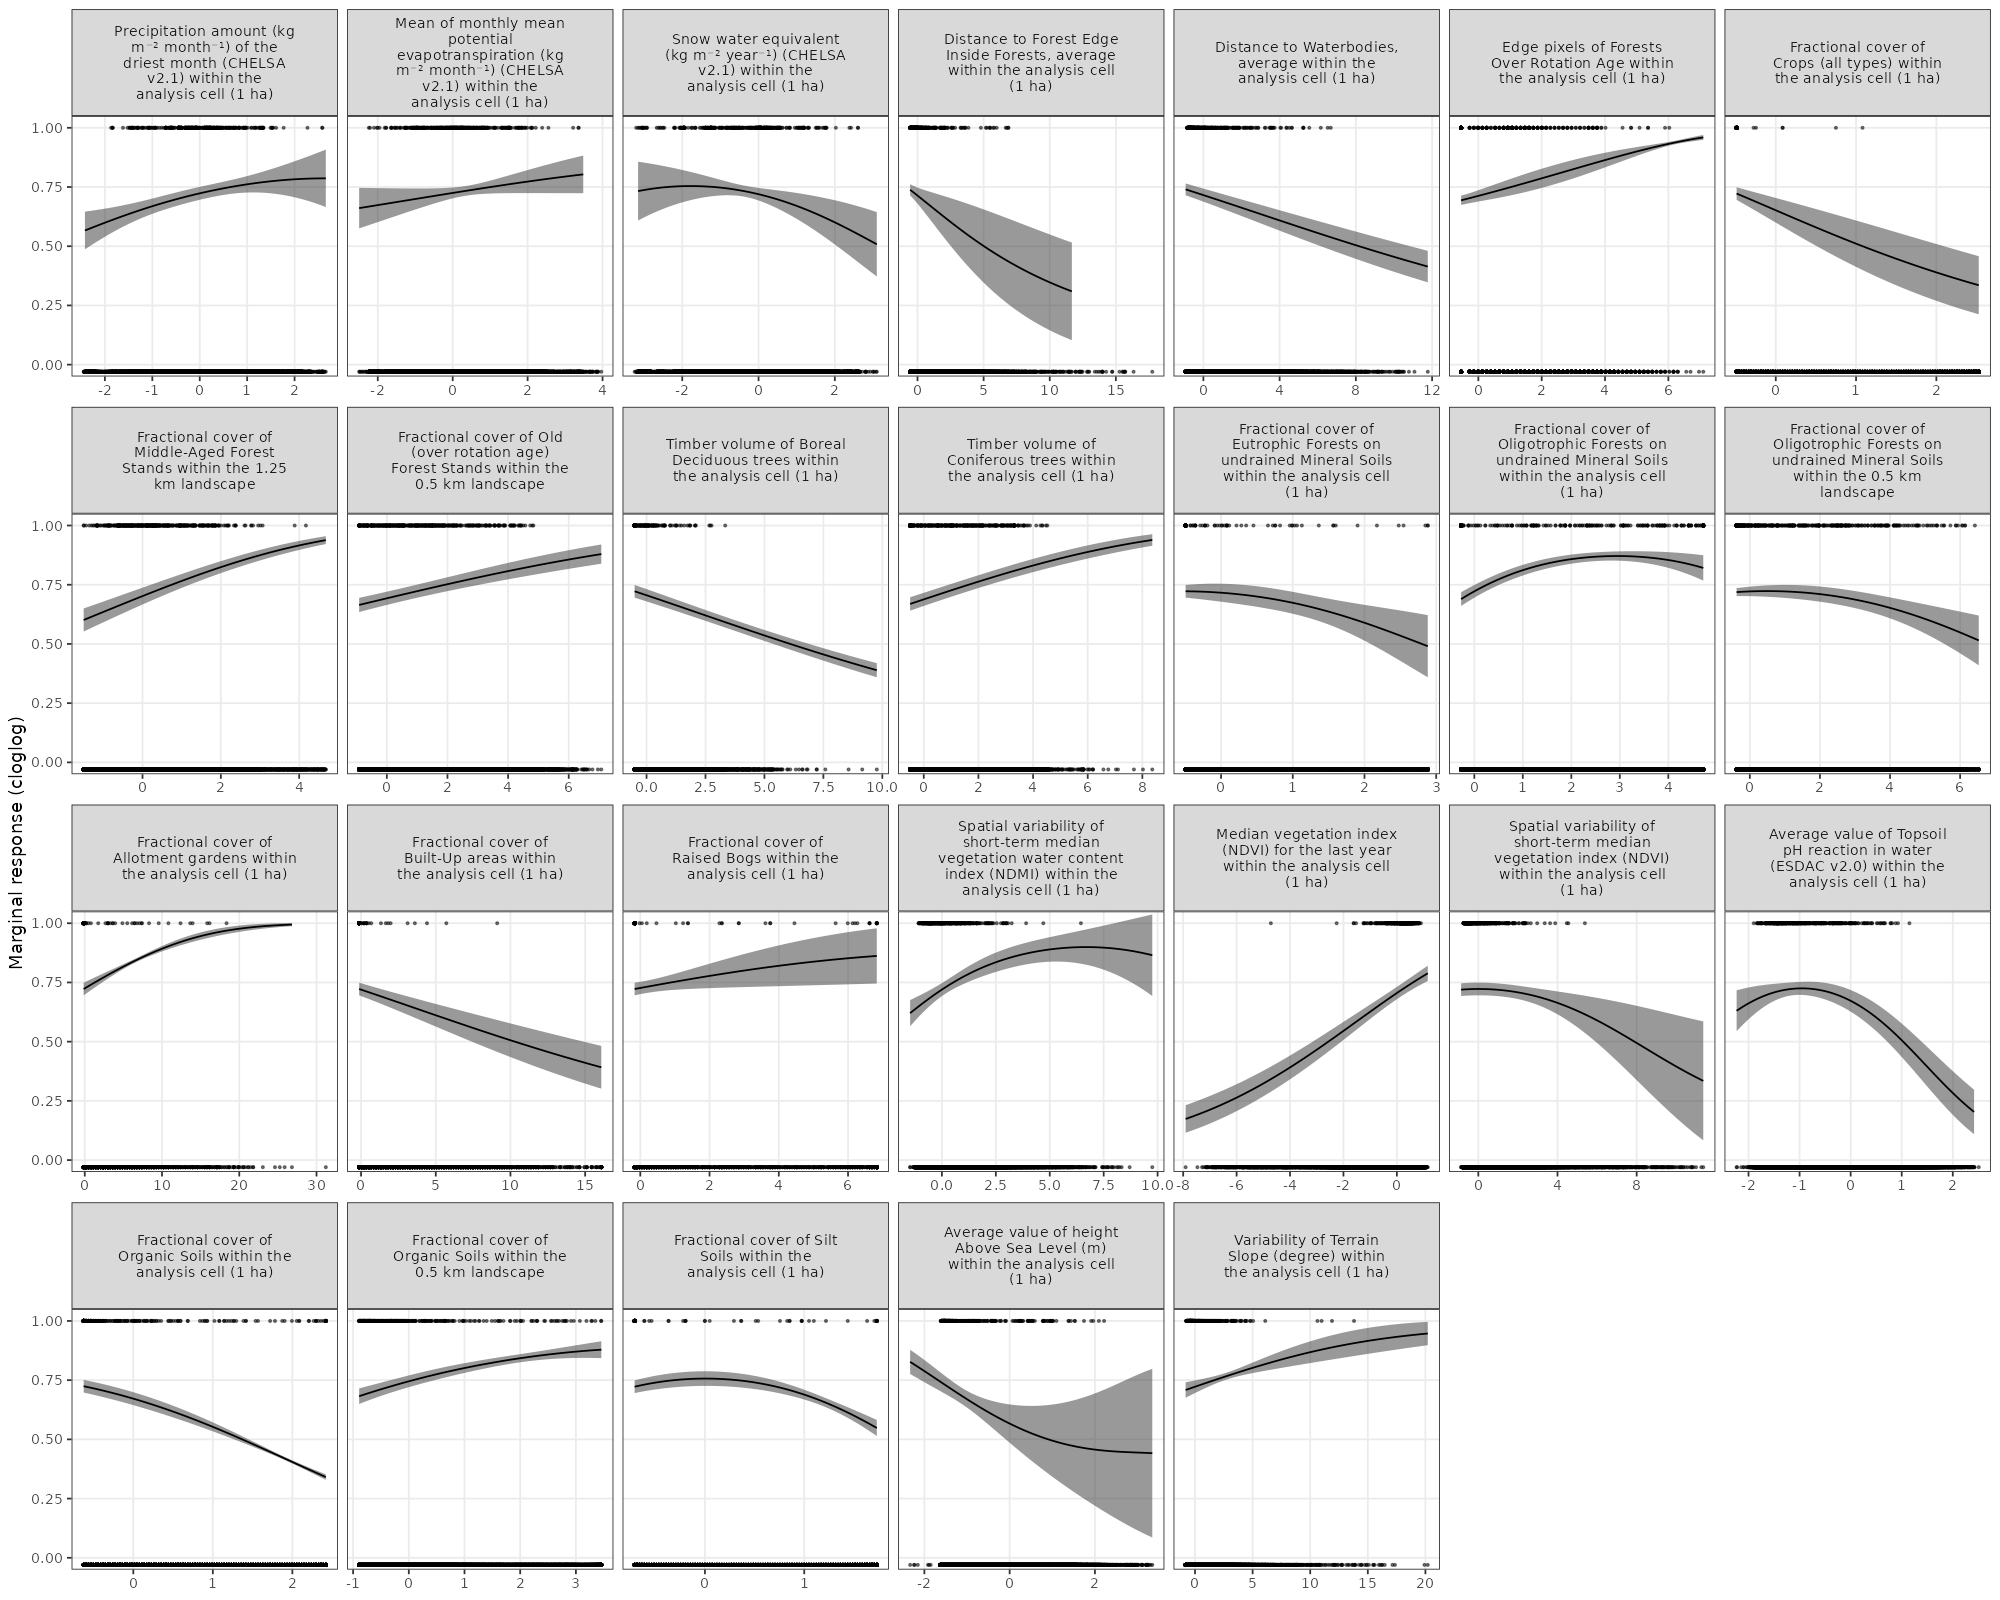
\includegraphics[width=1\linewidth,height=0.70\textheight,keepaspectratio]{results/ANGSPPv2b/PicMargResp_ANGSPP.png}

\par\small\textit{Marginalised for arithmetic mean response curves illustrating the effect of each ecogeographical variable on the habitat suitability when all the other variables have their arithmetic mean values. The y-axis shows the predicted habitat suitability (cloglog-transformed), while the x-axis shows the standardised (centred and scaled) value of the ecogeographical variable. Dots at a value of 1 on the y-axis illustrate presence locations in the environment (on the x-axis), while dots at a value of 0 illustrate background locations used in modelling.  **For a full resolution refer to repository: link or online document: link**}\normalsize
\end{center}

\section*{Habitat and conservation associations}\label{habitat-and-conservation-associations-28}
\addcontentsline{toc}{section}{Habitat and conservation associations}

\begin{center}
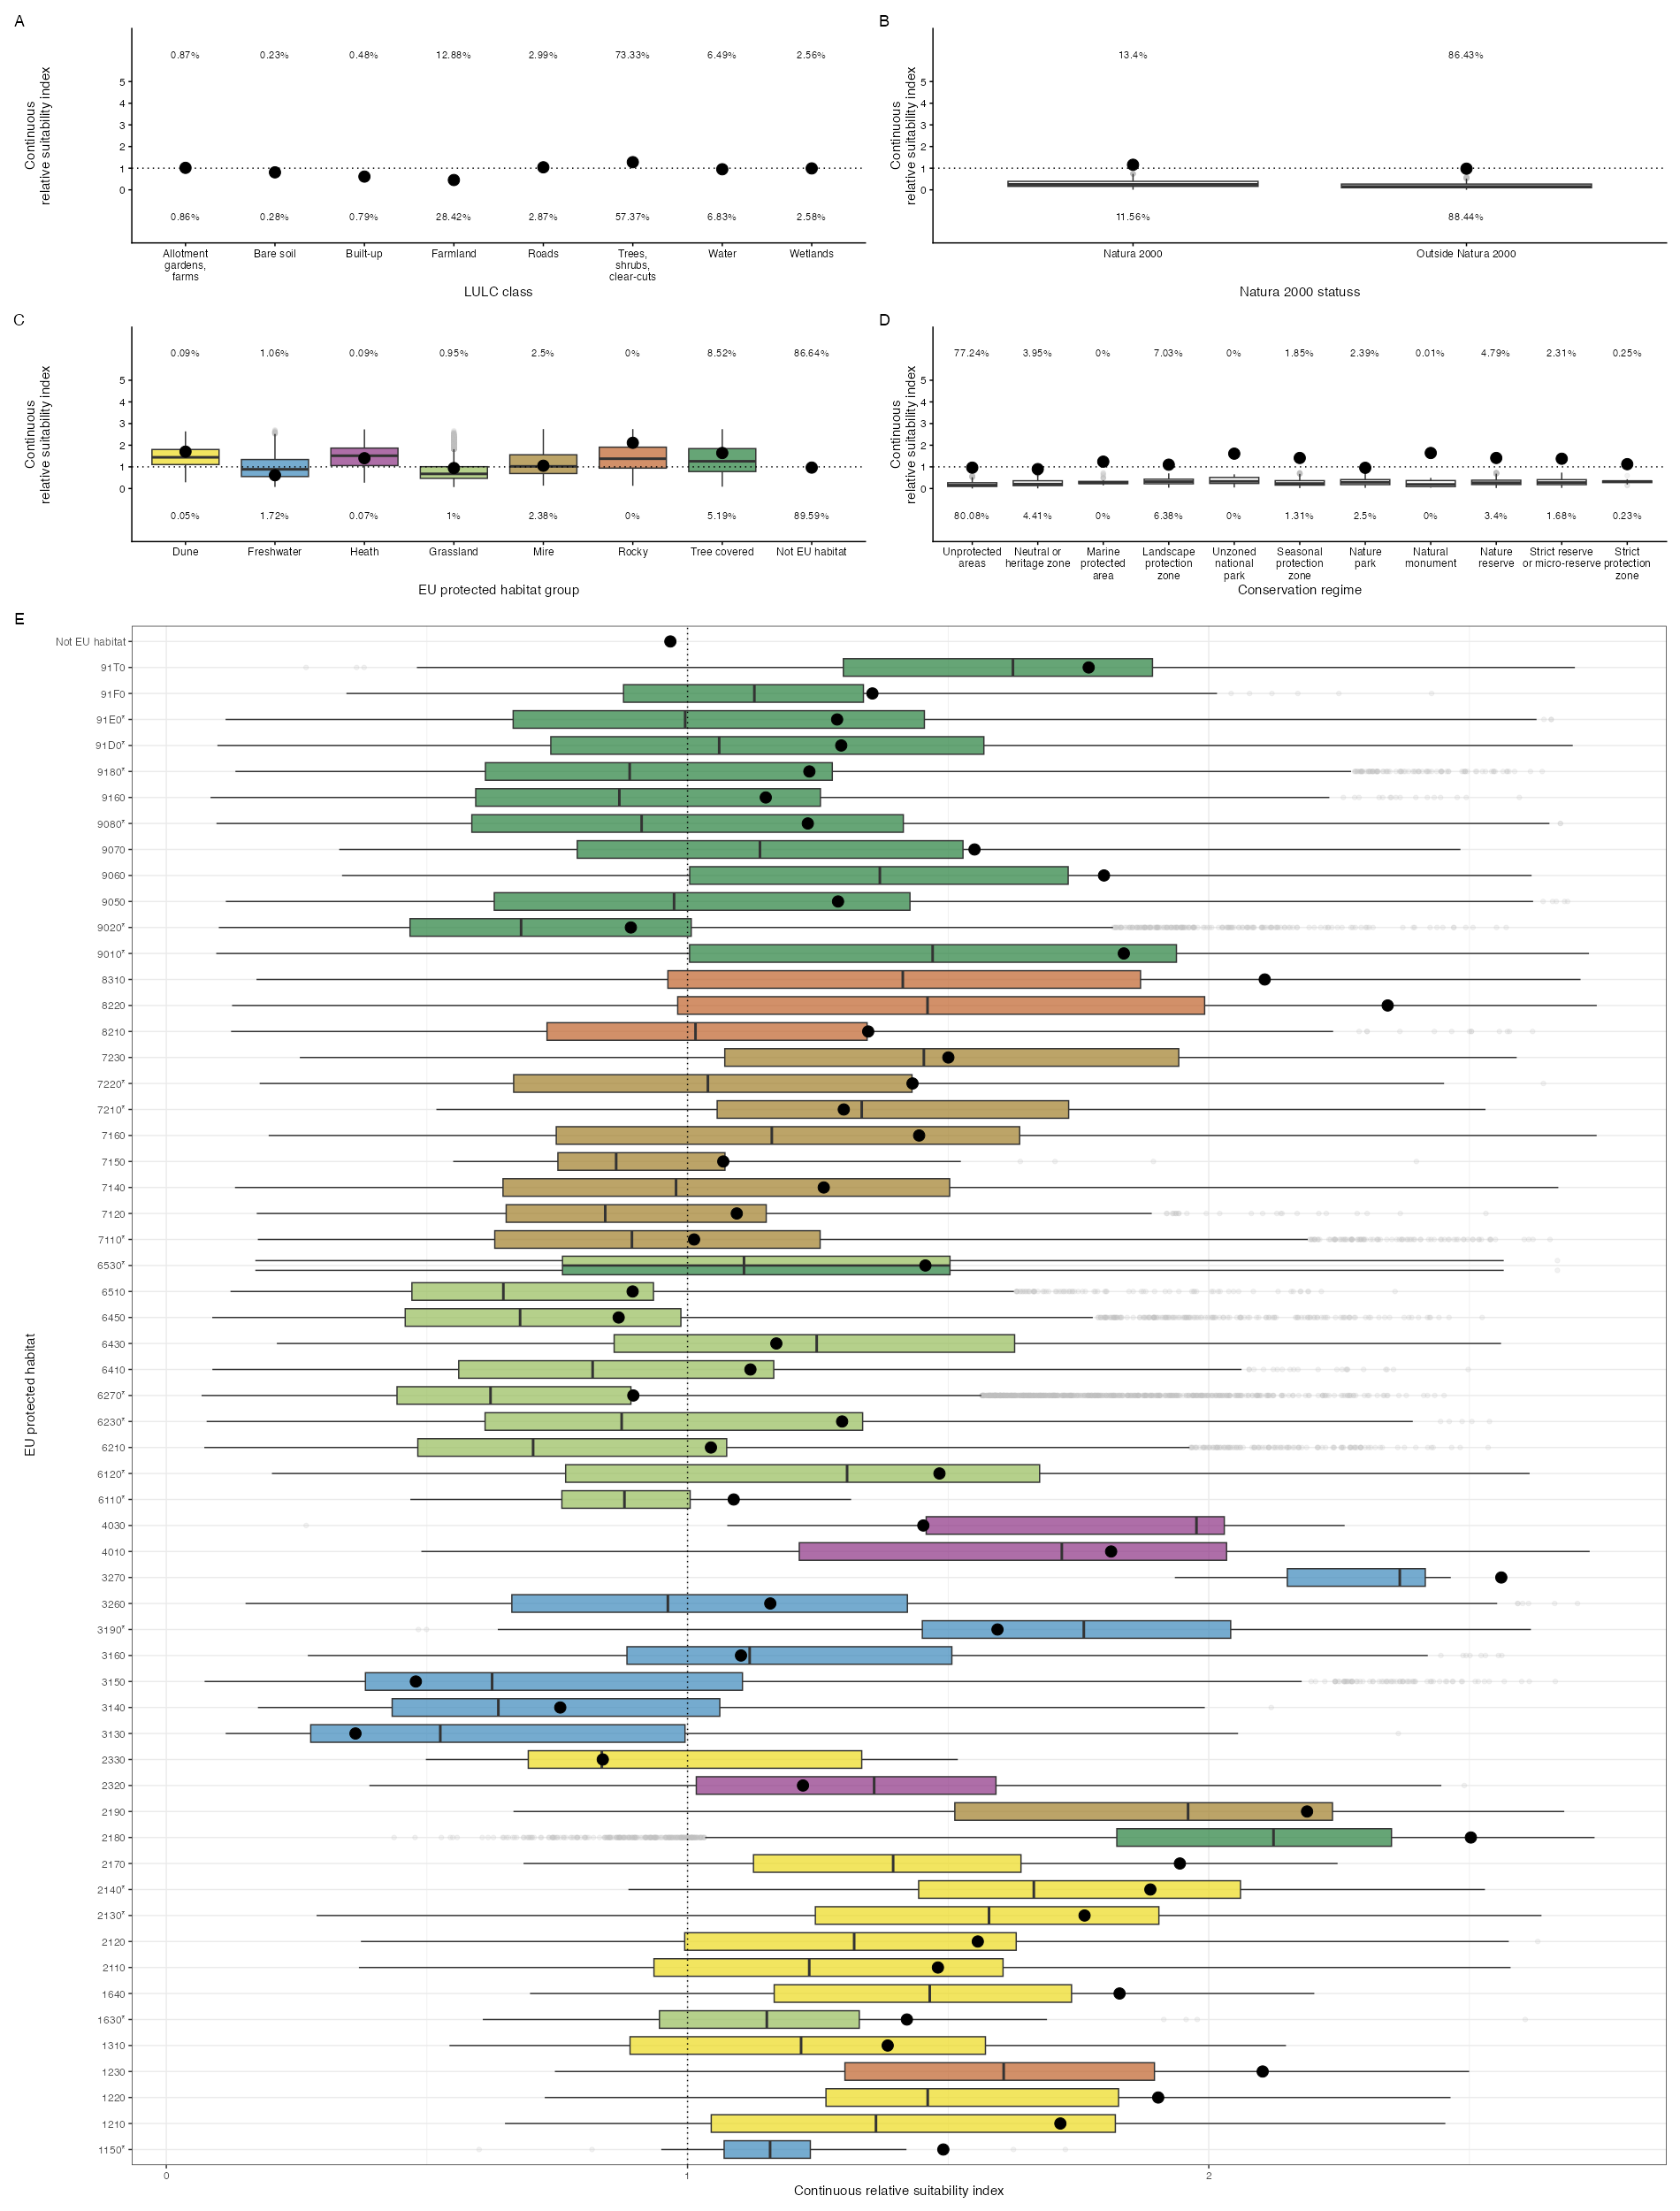
\includegraphics[width=1\linewidth,height=0.70\textheight,keepaspectratio]{results/ANGSPPv2b/PicAssoc_ANGSPP.png}

\par\small\textit{Associations between predicted suitability and: (A) land use land cover classes, (B) Natura 2000 status, (C) stratified EU protected habitat classes, (D) conservation regime, and (E) EU protected habitats. The y-axis show continuous relative suitability index (derivative of Manly's index of preference). Colours in (C) and (E) correspond to stratified EU protected habitat classes. For classifications composed of multiple individual polygons, polygon-level indices were additionally calculated to show within-category variation. The figures therefore combine category-level estimates (points) with the distributions of polygon-level values (boxplots, where applicable). Labels above and below the panels report, respectively, the percentage of total predicted suitability and the percentage of mapped area represented by each category. **For a full resolution refer to repository: link or online document: link**}\normalsize
\end{center}

\section*{Conservation prioritization}\label{conservation-prioritization-28}
\addcontentsline{toc}{section}{Conservation prioritization}

\begin{center}
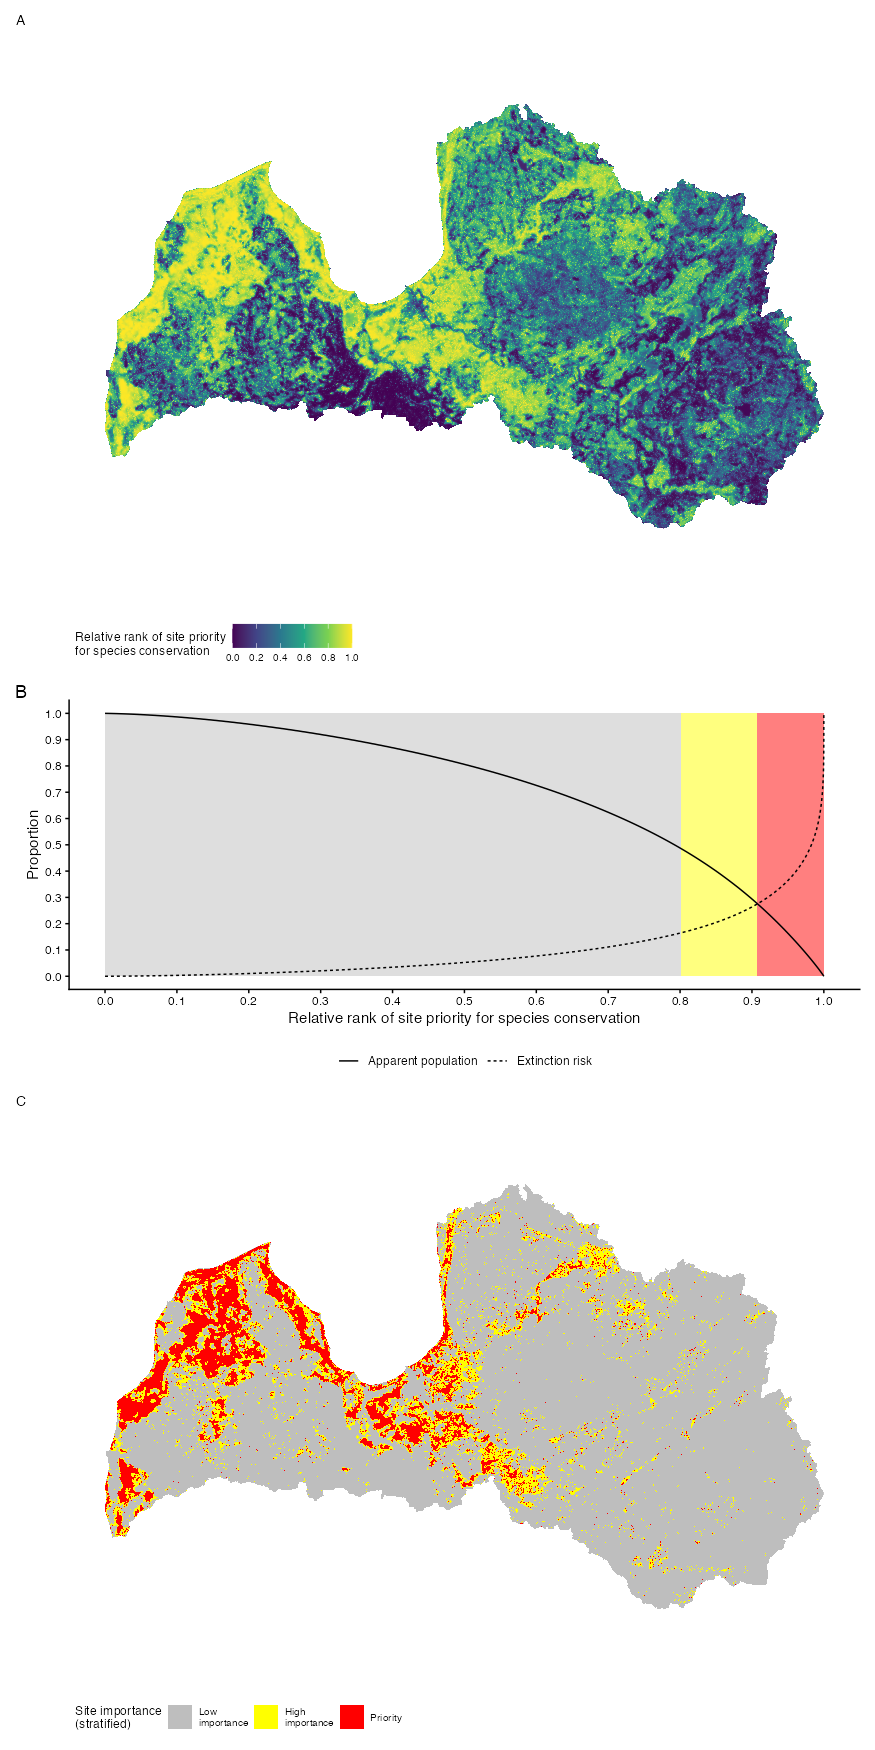
\includegraphics[width=0.85\linewidth,height=0.70\textheight,keepaspectratio]{results/ANGSPPv2b/PicPrior_ANGSPP.png}

\par\small\textit{Single-species conservation prioritization focusing on maximisation of core area protection (CAZMAX) while accounting for site connectivity: (A) relative site rank; (B) relationship between apparent-population and extinction-risk curves with a simplified classification which is spatially demonstrated in the bootom row; (C) spatial distribution of proposed classification of site prioritization results. **For a full resolution refer to repository: link or online document: link**}\normalsize
\end{center}

\protect\phantomsection\label{refs}
\begin{CSLReferences}{1}{1}
\bibitem[\citeproctext]{ref-Allouche2006TSS}
Allouche, Omri, Asaf Tsoar, and Ronen Kadmon. 2006. {``Assessing the Accuracy of Species Distribution Models: Prevalence, Kappa and the True Skill Statistic (TSS).''} \emph{Journal of Applied Ecology} 43: 1223--32. \url{https://doi.org/10.1111/j.1365-2664.2006.01214.x}.

\bibitem[\citeproctext]{ref-Avotins2026sdmhelpers}
Avotins, Andris. 2026. \emph{Sdmhelpers: Helper Functions for Species Distribution Modelling}. \url{https://github.com/aavotins/sdmhelpers}.

\bibitem[\citeproctext]{ref-AvotinsEtAl2025EGV}
Avotins, Andris, Jekaterīna Butkeviča, Betija Rubene, et al. 2025. {``High-Resolution Ecogeographical Variable Dataset Describing Latvia, 2024.''} Version 1.0.1. Zenodo. \url{https://doi.org/10.5281/zenodo.17805905}.

\bibitem[\citeproctext]{ref-DabasDati2026}
DabasDati.lv. 2026. \emph{DabasDati.lv: Nature Observation Portal}. \url{https://dabasdati.lv/en/dosearch/}.

\bibitem[\citeproctext]{ref-DormannEtAl2013Collinearity}
Dormann, Carsten F., Jane Elith, Sven Bacher, et al. 2013a. {``Collinearity: A Review of Methods to Deal with It and a Simulation Study Evaluating Their Performance.''} \emph{Ecography} 36 (1): 27--46. \url{https://doi.org/10.1111/j.1600-0587.2012.07348.x}.

\bibitem[\citeproctext]{ref-Dormann2013Collinearity}
Dormann, Carsten F., Jane Elith, Sven Bacher, et al. 2013b. {``Collinearity: A Review of Methods to Deal with It and a Simulation Study Evaluating Their Performance.''} \emph{Ecography} 36: 27--46. \url{https://doi.org/10.1111/j.1600-0587.2012.07348.x}.

\bibitem[\citeproctext]{ref-Elith2011MaxEnt}
Elith, Jane, Steven J. Phillips, Trevor Hastie, Miroslav Dudík, Yung En Chee, and Colin J. Yates. 2011. {``A Statistical Explanation of MaxEnt for Ecologists.''} \emph{Diversity and Distributions} 17: 43--57. \url{https://doi.org/10.1111/j.1472-4642.2010.00725.x}.

\bibitem[\citeproctext]{ref-FengEtAl2019Collinearity}
Feng, Xiao, Daniel S. Park, Yiyun Liang, Ram Pandey, and Monica Papes. 2019. {``Collinearity in Ecological Niche Modeling: Confusions and Challenges.''} \emph{Ecology and Evolution} 9 (18): 10365--76. \url{https://doi.org/10.1002/ece3.5555}.

\bibitem[\citeproctext]{ref-Fourcade2014Bias}
Fourcade, Yoan, Jan O. Engler, Dennis Rödder, and Jean Secondi. 2014. {``Mapping Species Distributions with MAXENT Using a Geographically Biased Sample of Presence Data: A Performance Assessment of Methods for Correcting Sampling Bias.''} \emph{PLOS ONE} 9 (5): e97122. \url{https://doi.org/10.1371/journal.pone.0097122}.

\bibitem[\citeproctext]{ref-Hijmans2012CrossValidation}
Hijmans, Robert J. 2012. {``Cross-Validation of Species Distribution Models: Removing Spatial Sorting Bias and Calibration with a Null Model.''} \emph{Ecology} 93: 679--88. \url{https://doi.org/10.1890/11-0826.1}.

\bibitem[\citeproctext]{ref-Hirzel2006Boyce}
Hirzel, Alexandre H., Gwenaëlle Le Lay, Véronique Helfer, Christophe Randin, and Antoine Guisan. 2006. {``Evaluating the Ability of Habitat Suitability Models to Predict Species Presences.''} \emph{Ecological Modelling} 199: 142--52. \url{https://doi.org/10.1016/j.ecolmodel.2006.05.017}.

\bibitem[\citeproctext]{ref-Kass2021ENMeval}
Kass, Jamie M., Robert Muscarella, Peter J. Galante, et al. 2021. {``ENMeval 2.0: Redesigned for Customizable and Reproducible Modeling of Species' Niches and Distributions.''} \emph{Methods in Ecology and Evolution} 12 (9): 1602--8. \url{https://doi.org/10.1111/2041-210X.13628}.

\bibitem[\citeproctext]{ref-LehtomakiMoilanen2013Workflow}
Lehtomäki, Joona, and Atte Moilanen. 2013. {``Methods and Workflow for Spatial Conservation Prioritization Using Zonation.''} \emph{Environmental Modelling \& Software} 47: 128--37. \url{https://doi.org/10.1016/j.envsoft.2013.05.001}.

\bibitem[\citeproctext]{ref-Lobo2008AUC}
Lobo, Jorge M., Alberto Jiménez-Valverde, and Raimundo Real. 2008. {``AUC: A Misleading Measure of the Performance of Predictive Distribution Models.''} \emph{Global Ecology and Biogeography} 17: 145--51. \url{https://doi.org/10.1111/j.1466-8238.2007.00358.x}.

\bibitem[\citeproctext]{ref-ManlyEtAl2002ResourceSelection}
Manly, Bryan F. J., Lyman L. McDonald, Dana L. Thomas, Trent L. McDonald, and Wallace P. Erickson. 2002. \emph{Resource Selection by Animals: Statistical Design and Analysis for Field Studies}. 2nd ed. Kluwer Academic Publishers.

\bibitem[\citeproctext]{ref-Merow2013MaxEntGuide}
Merow, Cory, Matthew J. Smith, and John A. Jr. Silander. 2013. {``A Practical Guide to MaxEnt for Modeling Species' Distributions: What It Does, and Why Inputs and Settings Matter.''} \emph{Ecography} 36: 1058--69. \url{https://doi.org/10.1111/j.1600-0587.2013.07872.x}.

\bibitem[\citeproctext]{ref-MoilanenEtAl2022Zonation5}
Moilanen, Atte, Pauli Lehtinen, Ilmari Kohonen, Joel Jalkanen, Elina A. Virtanen, and Heini Kujala. 2022. {``Novel Methods for Spatial Prioritization with Applications in Conservation, Land Use Planning and Ecological Impact Avoidance.''} \emph{Methods in Ecology and Evolution} 13 (5): 1062--72. \url{https://doi.org/10.1111/2041-210X.13819}.

\bibitem[\citeproctext]{ref-NatureConservationAgency2020OZOLS}
Nature Conservation Agency of the Republic of Latvia. 2020. \emph{Nature Data Management System OZOLS}. \url{https://www.daba.gov.lv/en/nature-data-management-system-ozols}.

\bibitem[\citeproctext]{ref-Phillips2009Bias}
Phillips, Steven J., Miroslav Dudík, Jane Elith, et al. 2009. {``Sample Selection Bias and Presence-Only Distribution Models: Implications for Background and Pseudo-Absence Data.''} \emph{Ecological Applications} 19: 181--97. \url{https://doi.org/10.1890/07-2153.1}.

\bibitem[\citeproctext]{ref-Radosavljevic2014Maxent}
Radosavljevic, Aleksandar, and Robert P. Anderson. 2014. {``Making Better Maxent Models of Species Distributions: Complexity, Overfitting and Evaluation.''} \emph{Journal of Biogeography} 41: 629--43. \url{https://doi.org/10.1111/jbi.12227}.

\bibitem[\citeproctext]{ref-Raes2007Null}
Raes, Niels, and Hans ter Steege. 2007. {``A Null-Model for Significance Testing of Presence-Only Species Distribution Models.''} \emph{Ecography} 30: 727--36. \url{https://doi.org/10.1111/j.2007.0906-7590.05041.x}.

\bibitem[\citeproctext]{ref-Roberts2017CrossValidation}
Roberts, David R., Volker Bahn, Simone Ciuti, et al. 2017. {``Cross-Validation Strategies for Data with Temporal, Spatial, Hierarchical, or Phylogenetic Structure.''} \emph{Ecography} 40: 913--29. \url{https://doi.org/10.1111/ecog.02881}.

\bibitem[\citeproctext]{ref-StarkaEtAl2026SpeciesDataset}
Starka, Rūta, Liene Auniņa, Maksims Balalaikins, et al. 2026. {``Species Dataset for Model-Based Conservation Planning in Latvia: Occurrences, Importance for Nature Conservation Planning and Ecogeographical Variable Selection.''} Version 2.0.1. Zenodo. \url{https://doi.org/10.5281/zenodo.21776959}.

\bibitem[\citeproctext]{ref-Valavi2019blockCV}
Valavi, Roozbeh, Jane Elith, José J. Lahoz-Monfort, and Gurutzeta Guillera-Arroita. 2019. {``blockCV: An r Package for Generating Spatially or Environmentally Separated Folds for k-Fold Cross-Validation of Species Distribution Models.''} \emph{Methods in Ecology and Evolution} 10: 225--32. \url{https://doi.org/10.1111/2041-210X.13107}.

\bibitem[\citeproctext]{ref-Vignali2020SDMtune}
Vignali, Sergio, Arnaud G. Barras, Raphaël Arlettaz, and Veronika Braunisch. 2020. {``SDMtune: An r Package to Tune and Evaluate Species Distribution Models.''} \emph{Ecology and Evolution} 10 (20): 11488--506. \url{https://doi.org/10.1002/ece3.6786}.

\bibitem[\citeproctext]{ref-Warren2011MaxentComplexity}
Warren, Dan L., and Stephanie N. Seifert. 2011. {``Ecological Niche Modeling in Maxent: The Importance of Model Complexity and the Performance of Model Selection Criteria.''} \emph{Ecological Applications} 21: 335--42. \url{https://doi.org/10.1890/10-1171.1}.

\end{CSLReferences}

\end{document}
